% Options for packages loaded elsewhere
\PassOptionsToPackage{unicode}{hyperref}
\PassOptionsToPackage{hyphens}{url}
%
\documentclass[
  a4paper,
]{scrbook}

\usepackage{amsmath,amssymb}
\usepackage{iftex}
\ifPDFTeX
  \usepackage[T1]{fontenc}
  \usepackage[utf8]{inputenc}
  \usepackage{textcomp} % provide euro and other symbols
\else % if luatex or xetex
  \usepackage{unicode-math}
  \defaultfontfeatures{Scale=MatchLowercase}
  \defaultfontfeatures[\rmfamily]{Ligatures=TeX,Scale=1}
\fi
\usepackage{lmodern}
\ifPDFTeX\else  
    % xetex/luatex font selection
\fi
% Use upquote if available, for straight quotes in verbatim environments
\IfFileExists{upquote.sty}{\usepackage{upquote}}{}
\IfFileExists{microtype.sty}{% use microtype if available
  \usepackage[]{microtype}
  \UseMicrotypeSet[protrusion]{basicmath} % disable protrusion for tt fonts
}{}
\makeatletter
\@ifundefined{KOMAClassName}{% if non-KOMA class
  \IfFileExists{parskip.sty}{%
    \usepackage{parskip}
  }{% else
    \setlength{\parindent}{0pt}
    \setlength{\parskip}{6pt plus 2pt minus 1pt}}
}{% if KOMA class
  \KOMAoptions{parskip=half}}
\makeatother
\usepackage{xcolor}
\setlength{\emergencystretch}{3em} % prevent overfull lines
\setcounter{secnumdepth}{3}
% Make \paragraph and \subparagraph free-standing
\ifx\paragraph\undefined\else
  \let\oldparagraph\paragraph
  \renewcommand{\paragraph}[1]{\oldparagraph{#1}\mbox{}}
\fi
\ifx\subparagraph\undefined\else
  \let\oldsubparagraph\subparagraph
  \renewcommand{\subparagraph}[1]{\oldsubparagraph{#1}\mbox{}}
\fi

\usepackage{color}
\usepackage{fancyvrb}
\newcommand{\VerbBar}{|}
\newcommand{\VERB}{\Verb[commandchars=\\\{\}]}
\DefineVerbatimEnvironment{Highlighting}{Verbatim}{commandchars=\\\{\}}
% Add ',fontsize=\small' for more characters per line
\usepackage{framed}
\definecolor{shadecolor}{RGB}{241,243,245}
\newenvironment{Shaded}{\begin{snugshade}}{\end{snugshade}}
\newcommand{\AlertTok}[1]{\textcolor[rgb]{0.68,0.00,0.00}{#1}}
\newcommand{\AnnotationTok}[1]{\textcolor[rgb]{0.37,0.37,0.37}{#1}}
\newcommand{\AttributeTok}[1]{\textcolor[rgb]{0.40,0.45,0.13}{#1}}
\newcommand{\BaseNTok}[1]{\textcolor[rgb]{0.68,0.00,0.00}{#1}}
\newcommand{\BuiltInTok}[1]{\textcolor[rgb]{0.00,0.23,0.31}{#1}}
\newcommand{\CharTok}[1]{\textcolor[rgb]{0.13,0.47,0.30}{#1}}
\newcommand{\CommentTok}[1]{\textcolor[rgb]{0.37,0.37,0.37}{#1}}
\newcommand{\CommentVarTok}[1]{\textcolor[rgb]{0.37,0.37,0.37}{\textit{#1}}}
\newcommand{\ConstantTok}[1]{\textcolor[rgb]{0.56,0.35,0.01}{#1}}
\newcommand{\ControlFlowTok}[1]{\textcolor[rgb]{0.00,0.23,0.31}{#1}}
\newcommand{\DataTypeTok}[1]{\textcolor[rgb]{0.68,0.00,0.00}{#1}}
\newcommand{\DecValTok}[1]{\textcolor[rgb]{0.68,0.00,0.00}{#1}}
\newcommand{\DocumentationTok}[1]{\textcolor[rgb]{0.37,0.37,0.37}{\textit{#1}}}
\newcommand{\ErrorTok}[1]{\textcolor[rgb]{0.68,0.00,0.00}{#1}}
\newcommand{\ExtensionTok}[1]{\textcolor[rgb]{0.00,0.23,0.31}{#1}}
\newcommand{\FloatTok}[1]{\textcolor[rgb]{0.68,0.00,0.00}{#1}}
\newcommand{\FunctionTok}[1]{\textcolor[rgb]{0.28,0.35,0.67}{#1}}
\newcommand{\ImportTok}[1]{\textcolor[rgb]{0.00,0.46,0.62}{#1}}
\newcommand{\InformationTok}[1]{\textcolor[rgb]{0.37,0.37,0.37}{#1}}
\newcommand{\KeywordTok}[1]{\textcolor[rgb]{0.00,0.23,0.31}{#1}}
\newcommand{\NormalTok}[1]{\textcolor[rgb]{0.00,0.23,0.31}{#1}}
\newcommand{\OperatorTok}[1]{\textcolor[rgb]{0.37,0.37,0.37}{#1}}
\newcommand{\OtherTok}[1]{\textcolor[rgb]{0.00,0.23,0.31}{#1}}
\newcommand{\PreprocessorTok}[1]{\textcolor[rgb]{0.68,0.00,0.00}{#1}}
\newcommand{\RegionMarkerTok}[1]{\textcolor[rgb]{0.00,0.23,0.31}{#1}}
\newcommand{\SpecialCharTok}[1]{\textcolor[rgb]{0.37,0.37,0.37}{#1}}
\newcommand{\SpecialStringTok}[1]{\textcolor[rgb]{0.13,0.47,0.30}{#1}}
\newcommand{\StringTok}[1]{\textcolor[rgb]{0.13,0.47,0.30}{#1}}
\newcommand{\VariableTok}[1]{\textcolor[rgb]{0.07,0.07,0.07}{#1}}
\newcommand{\VerbatimStringTok}[1]{\textcolor[rgb]{0.13,0.47,0.30}{#1}}
\newcommand{\WarningTok}[1]{\textcolor[rgb]{0.37,0.37,0.37}{\textit{#1}}}

\providecommand{\tightlist}{%
  \setlength{\itemsep}{0pt}\setlength{\parskip}{0pt}}\usepackage{longtable,booktabs,array}
\usepackage{calc} % for calculating minipage widths
% Correct order of tables after \paragraph or \subparagraph
\usepackage{etoolbox}
\makeatletter
\patchcmd\longtable{\par}{\if@noskipsec\mbox{}\fi\par}{}{}
\makeatother
% Allow footnotes in longtable head/foot
\IfFileExists{footnotehyper.sty}{\usepackage{footnotehyper}}{\usepackage{footnote}}
\makesavenoteenv{longtable}
\usepackage{graphicx}
\makeatletter
\def\maxwidth{\ifdim\Gin@nat@width>\linewidth\linewidth\else\Gin@nat@width\fi}
\def\maxheight{\ifdim\Gin@nat@height>\textheight\textheight\else\Gin@nat@height\fi}
\makeatother
% Scale images if necessary, so that they will not overflow the page
% margins by default, and it is still possible to overwrite the defaults
% using explicit options in \includegraphics[width, height, ...]{}
\setkeys{Gin}{width=\maxwidth,height=\maxheight,keepaspectratio}
% Set default figure placement to htbp
\makeatletter
\def\fps@figure{htbp}
\makeatother

\usepackage{libertine}
\providecommand{\ped}[1]{_\textrm{#1}}
\providecommand{\ap}[1]{^\textrm{#1}}
\providecommand{\app}[1]{^\textrm{#1}}

\providecommand*{\angs}{\smash{\mathrm{\ring A}}}
\providecommand*{\celsius}{\mathrm{~\circ C}}
\providecommand*{\micro}{\mu}

\providecommand*{\unit}[1]{\textrm{\,#1}}


\providecommand{\E}{\mathrm{e}}
\providecommand{\I}{\mathrm{i}}
\providecommand{\sfrac}[2]{^{#1}/_{#2}}

\providecommand{\conc}[1]{\left[\mathrm{#1}\right]}


\providecommand{\command}[1]{\textsl{#1}}
\providecommand{\out}[1]{\begin{verbatim}#1\end{verbatim}}


\providecommand{\diff}{\mathrm{d}\,}


\providecommand*{\deriv}[3][]{% arguments: order of the derivative(optional), function, variable
	\frac{\diff^{#1}#2}{\diff #3^{#1}}}
\providecommand*{\pderiv}[3][]{% arguments: order of the derivative(optional), function, variable
	\frac{\partial^{#1}#2}
		{\partial #3^{#1}}}
  
\renewcommand{\vec}[1]{{\boldsymbol #1}}

\providecommand{\cov}[2]{\mathrm{Cov}\!\left(#1, #2\right)}
\providecommand{\var}[1]{\mathrm{Var}\!\left(#1\right)}

\providecommand{\mean}[1]{\overline{#1}}

\providecommand{\sd}[1]{\sigma\left(#1\right)}
\providecommand{\ev}[1]{\mathbb{E}\!\left(#1\right)}
\providecommand{\pr}[1]{\textrm{Pr}\!\left(#1\right)}

\makeatletter
\@ifpackageloaded{tcolorbox}{}{\usepackage[skins,breakable]{tcolorbox}}
\@ifpackageloaded{fontawesome5}{}{\usepackage{fontawesome5}}
\definecolor{quarto-callout-color}{HTML}{909090}
\definecolor{quarto-callout-note-color}{HTML}{0758E5}
\definecolor{quarto-callout-important-color}{HTML}{CC1914}
\definecolor{quarto-callout-warning-color}{HTML}{EB9113}
\definecolor{quarto-callout-tip-color}{HTML}{00A047}
\definecolor{quarto-callout-caution-color}{HTML}{FC5300}
\definecolor{quarto-callout-color-frame}{HTML}{acacac}
\definecolor{quarto-callout-note-color-frame}{HTML}{4582ec}
\definecolor{quarto-callout-important-color-frame}{HTML}{d9534f}
\definecolor{quarto-callout-warning-color-frame}{HTML}{f0ad4e}
\definecolor{quarto-callout-tip-color-frame}{HTML}{02b875}
\definecolor{quarto-callout-caution-color-frame}{HTML}{fd7e14}
\makeatother
\makeatletter
\makeatother
\makeatletter
\makeatother
\makeatletter
\@ifpackageloaded{caption}{}{\usepackage{caption}}
\AtBeginDocument{%
\ifdefined\contentsname
  \renewcommand*\contentsname{Inhoudsopgave}
\else
  \newcommand\contentsname{Inhoudsopgave}
\fi
\ifdefined\listfigurename
  \renewcommand*\listfigurename{Lijst van figuren}
\else
  \newcommand\listfigurename{Lijst van figuren}
\fi
\ifdefined\listtablename
  \renewcommand*\listtablename{Lijst van tabellen}
\else
  \newcommand\listtablename{Lijst van tabellen}
\fi
\ifdefined\figurename
  \renewcommand*\figurename{Figuur}
\else
  \newcommand\figurename{Figuur}
\fi
\ifdefined\tablename
  \renewcommand*\tablename{Tabel}
\else
  \newcommand\tablename{Tabel}
\fi
}
\@ifpackageloaded{float}{}{\usepackage{float}}
\floatstyle{ruled}
\@ifundefined{c@chapter}{\newfloat{codelisting}{h}{lop}}{\newfloat{codelisting}{h}{lop}[chapter]}
\floatname{codelisting}{Listing}
\newcommand*\listoflistings{\listof{codelisting}{Lijst van listings}}
\usepackage{amsthm}
\theoremstyle{definition}
\newtheorem{exercise}{Oefening}[chapter]
\theoremstyle{remark}
\AtBeginDocument{\renewcommand*{\proofname}{Bewijs}}
\newtheorem*{remark}{Opmerking}
\newtheorem*{solution}{Oplossing}
\makeatother
\makeatletter
\@ifpackageloaded{caption}{}{\usepackage{caption}}
\@ifpackageloaded{subcaption}{}{\usepackage{subcaption}}
\makeatother
\makeatletter
\@ifpackageloaded{tcolorbox}{}{\usepackage[skins,breakable]{tcolorbox}}
\makeatother
\makeatletter
\@ifundefined{shadecolor}{\definecolor{shadecolor}{rgb}{.97, .97, .97}}
\makeatother
\makeatletter
\makeatother
\makeatletter
\makeatother
\ifLuaTeX
\usepackage[bidi=basic]{babel}
\else
\usepackage[bidi=default]{babel}
\fi
\babelprovide[main,import]{dutch}
% get rid of language-specific shorthands (see #6817):
\let\LanguageShortHands\languageshorthands
\def\languageshorthands#1{}
\ifLuaTeX
  \usepackage{selnolig}  % disable illegal ligatures
\fi
\IfFileExists{bookmark.sty}{\usepackage{bookmark}}{\usepackage{hyperref}}
\IfFileExists{xurl.sty}{\usepackage{xurl}}{} % add URL line breaks if available
\urlstyle{same} % disable monospaced font for URLs
\hypersetup{
  pdftitle={Kwantitatieve Biologie},
  pdfauthor={Vakgroep Biologie, Universiteit Utrecht},
  pdflang={nl},
  hidelinks,
  pdfcreator={LaTeX via pandoc}}

\title{Kwantitatieve Biologie}
\author{Vakgroep Biologie, Universiteit Utrecht}
\date{2024-06-20}

\begin{document}
\frontmatter
\maketitle
\ifdefined\Shaded\renewenvironment{Shaded}{\begin{tcolorbox}[boxrule=0pt, breakable, sharp corners, frame hidden, interior hidden, enhanced, borderline west={3pt}{0pt}{shadecolor}]}{\end{tcolorbox}}\fi

\renewcommand*\contentsname{Inhoudsopgave}
{
\setcounter{tocdepth}{1}
\tableofcontents
}
\mainmatter
\part{Inleiding}

Biologie is een wetenschap die te maken heeft met veel onderdeeltjes, en
allemaal van hele verschillende schalen. We bestuderen nucleotiden,
eiwitten, organellen, cellen, weefsels, organen, organismen, en
ecosystemen, wat samengenomen een schaalvergroting is van meerdere
biljoenen. Om deze complexe systemen te begrijpen, kunnen we enerzijds
proberen deze te versimpelen (modelleren), of anderzijds goed te leren
omgaan met (grote hoeveelheden) data. Deze cursus is er op gericht om
iedere bioloog de grondbeginselen bij te brengen van deze twee
strategiën: modelleren en statistiek.

\hypertarget{algemene-inleiding-cursus}{%
\chapter{Algemene inleiding cursus}\label{algemene-inleiding-cursus}}

Ik ben een algemene inleiding hoor.

\part{Basisprincipes van R}

\hypertarget{introductie-en-installatie}{%
\chapter{Introductie en installatie}\label{introductie-en-installatie}}

Biologie in de 21e eeuw vereist analyse van grote hoeveelheden data, en
modellering om complexe biologische systemen beter te begrijpen en te
voorspellen. In dit onderdeel van de cursus maak je kort kennis met de
basisprincipes van R, zodat ook jij straks voorspellingen kan doen, kan
aantonen of een gemeten verschil statistisch significant is, en mooie
grafieken kan maken.

\begin{figure}

{\centering \includegraphics{Programmeren/figuren/rfrogs.png}

}

\caption{\label{fig-phrogs}Om kikkers te begrijpen kunnen we niet alleen
heel hard naar kikkers kijken (afbeelding gegenereerd met Dall-E, juli
2024)}

\end{figure}

\hypertarget{beginnen-met-rstudio}{%
\section{Beginnen met Rstudio}\label{beginnen-met-rstudio}}

\begin{figure}

{\centering 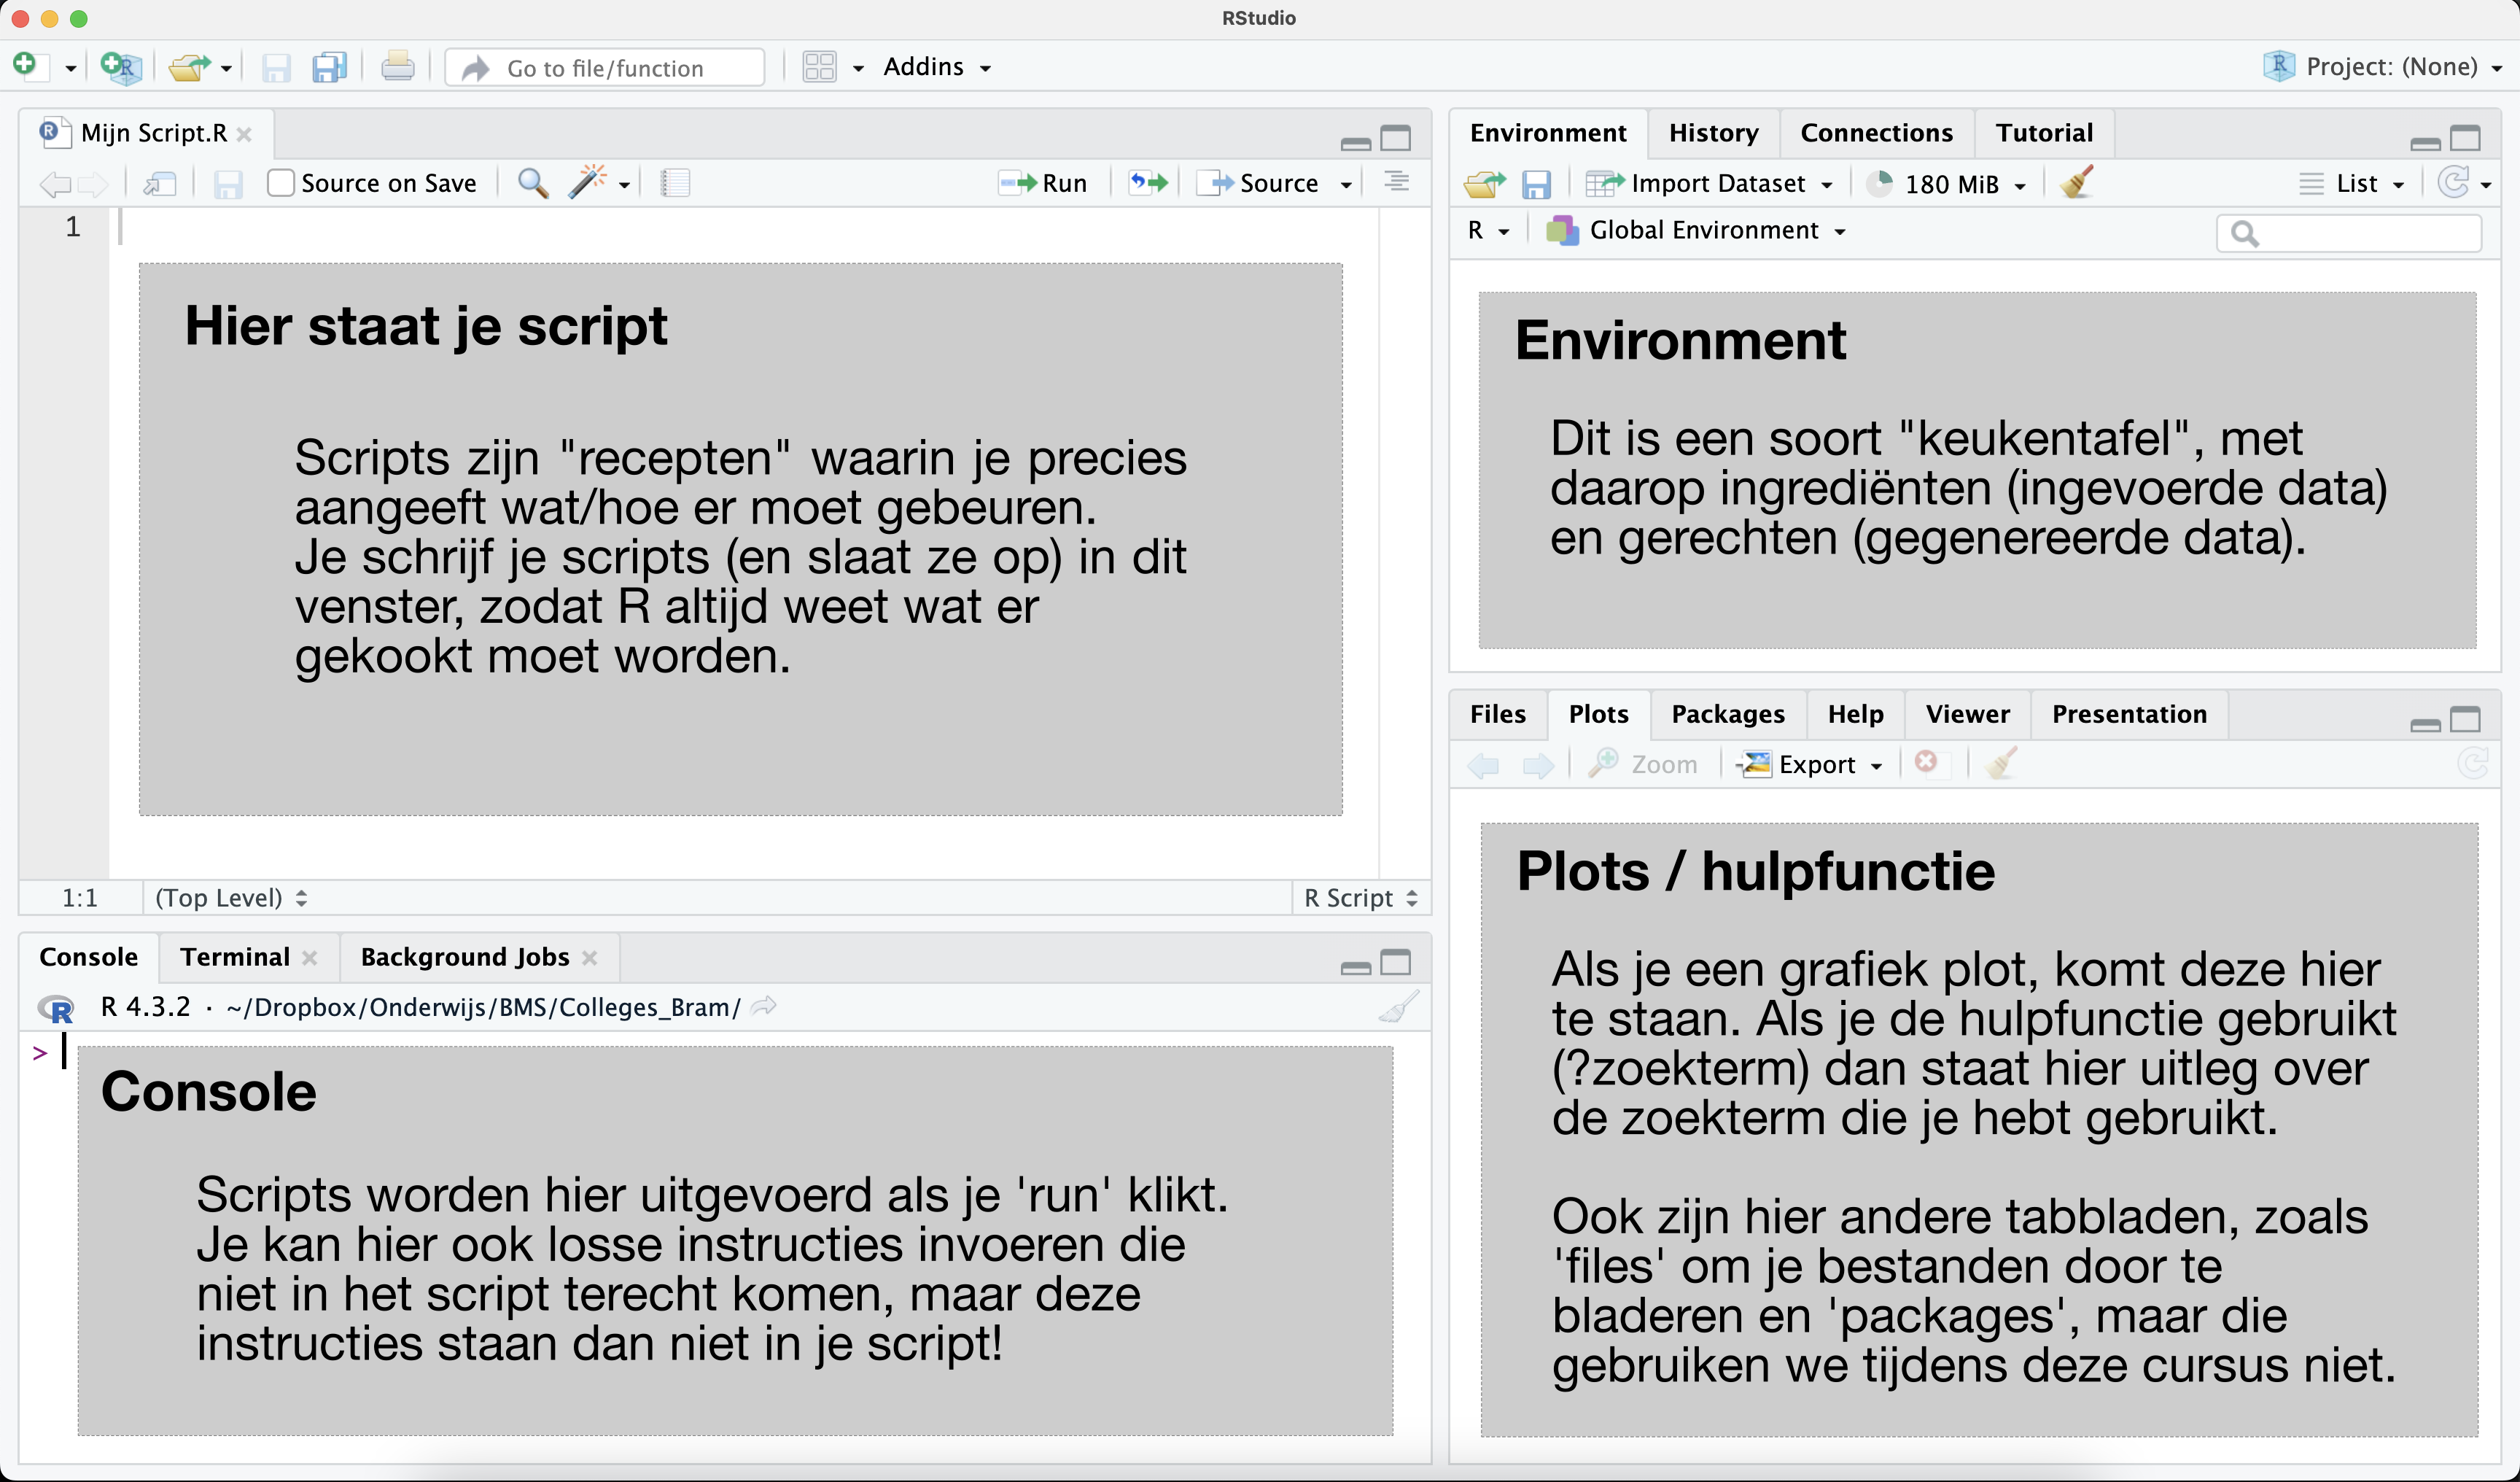
\includegraphics[width=0.5\textwidth,height=\textheight]{Programmeren/figuren/Rstudio.png}

}

\end{figure}

Er bestaan heel veel verschillende programmeertalen. Misschien heb je
weleens gehoord van Python, C, of Javascript. Het analyseren van grote
datasets wordt door biologen echter veelal in de programmeertaal R
gedaan, omdat deze makkelijk te installeren is door het grote aantal
gebruikers is er op internet gemakkelijk hulp te vinden. Daarom gaan
jullie tijdens deze cursus met Rstudio leren programmeren, een programma
dat je relatief eenvoudig kan installeren op je laptop. Maar eerst
moeten we nog even R zelf installeren.

\hypertarget{r-zelf-installeren}{%
\section{R zelf installeren}\label{r-zelf-installeren}}

R kun je eenvoudig installeren. Het is te vinden op de
\href{https://cran.r-project.org/}{CRAN website}, en de instructies voor
Mac en Windows gebruikers zijn daar ook te vinden:

\begin{itemize}
\item
  Windows-gebruikers: ga naar ``Download R for Windows'', klikken op de
  link ``base'' en vervolgens op de link ``Download R x.x.x for
  Windows'' om het installatiebestand te downloaden. Open het
  gedownloadde \texttt{.exe} bestand en volg de instructies om R te
  installeren.
\item
  Mac-gebruikers: ``Download R for (Mac) OS X''. Download het juiste
  installatiebestand voor jouw macOS-versie. Let op: als je een oudere
  Mac gebruikt moet je de ``Intel Mac'' versie downloaden. Open het .pkg
  bestand en volg de instructies.
\end{itemize}

\hypertarget{r-studio-installeren}{%
\section{R-studio installeren}\label{r-studio-installeren}}

Nadat je R geïnstalleerd hebt, kun je beginnen met het installeren van
Rstudio. Deze downloaden we vanaf de
\href{https://posit.co/download/rstudio-desktop/}{website van Rstudio}.
Deze website legt ook uit dat je wel eerst R moet installeren, maar dat
hebben we al gedaan. We kunnen dus meteen naar stap 2: Install Rstudio.
Deze website herkent vanzelf wel besturingssysteem je gebruikt, dus hoef
je het alleen nog maar te installeren:

\begin{itemize}
\item
  Windows-gebruikers: volg de instructies van de installatie-wizard
\item
  Mac-gebruiker: open de .dmg en sleep ``Rstudio'' naar je Applications
  folder
\end{itemize}

Nu kun je Rstudio opstarten, en zou alles moeten werken\footnote{In een
  enkel geval kan Rstudio de installatie van R niet automatisch vinden.
  Ga dan naar `Tools' \textgreater{} `Global options', en dan naar het
  tabblad `General'. Hier kan je handmatig instellen waar R
  geïnstalleerd staat. Vraag waar nodig hulp van je student-assistent
  (of ChatGPT ;{]})}

\hypertarget{je-eerste-script}{%
\section{Je eerste script}\label{je-eerste-script}}

Nu je Rstudio hebt opgestart, gaan we eerst een nieuw script aanmaken.
Ga hiervoor naar
\texttt{File\ -\textgreater{}\ New\ file\ -\textgreater{}\ R\ script}
(\texttt{Ctrl/Cmd+Shift+N}). Nu opent zich een nieuw venster, met daar
in een \texttt{script} zonder naam. Sla dit lege script op op een
logische plek op je computer. Maar wat is een script eigenlijk?

Een script is vergelijkbaar met een recept: het bevat de instructies om
iets lekkers te koken, maar niet de ingredienten of het resultaat zelf.
Deze instructies staan in zogeheten ``plain text'' formaat. Dit betekent
dat de tekst geen vetgedrukte woorden, cursief, onderstrepingen, kleuren
of speciale lettertypes bevat. Plain tekst kan data beschrijven
(bijvoorbeeld met elke regel een observatie), of in het geval van een
R-script een set van instructies. Elke regel bevat hoogstens 1
instructie, en deze code kan regel-per-regel worden uitgevoerd, of in
één keer.

Kopieer voor het volgende onderdeel de volgende code naar je eigen
script:

\begin{Shaded}
\begin{Highlighting}[]
\DecValTok{1}\SpecialCharTok{+}\DecValTok{2}
\DecValTok{1}\SpecialCharTok{+}\DecValTok{2{-}3}
\DecValTok{1}\SpecialCharTok{+}\DecValTok{2{-}3}\SpecialCharTok{*}\DecValTok{4}\SpecialCharTok{/}\DecValTok{5}
\end{Highlighting}
\end{Shaded}

\hypertarget{script-en-console}{%
\section{Script en console}\label{script-en-console}}

In Rstudio kun je op meerdere manieren regels code uitvoeren. Om de code
uit je script regel-per-regel uit te voeren, klik je de bovenste regel
aan (niet selecteren, maar gewoon ergens in de regel klikken), en
gebruik je de knop \texttt{Run} (de sneltoets hiervoor is
\texttt{Ctrl/Cmd+Enter}, wat heel handig is om in je vingers te
krijgen!). Nu je de eerste regel hebt uitgevoerd, zie je in de console
(onder het script) het antwoord: \texttt{{[}1{]}\ 3}. De
\texttt{{[}1{]}} geeft aan dat dit het eerste waarde is die de
berekening heeft gegeven. Omdat je maar 1 berekening hebt (1+2)
gevraagd, is dit dus ook het enige waarde. Later zul je zien dat een
berekening ook meerdere waarden terug kan geven. Je kan ook het hele
script in één keer uitvoeren door op \texttt{Source} te klikken. Als je
dit doet, zul je zien dat er regel voor regel antwoord word gegeven op
de sommetjes.

De bovenstaande uitleg geeft aan hoe je het script (het ``recept'') uit
kan voeren, maar wat nu als je even snel iets wil uitproberen voordat je
het recept helemaal overhoop gooit? Hiervoor kun je direct in de console
typen. Als je bijvoorbeeld de berekening \texttt{81/250} in de console
typt, heb je gauw een antwoord op je vraag maar is je script niet
aangepast. De console is dus handig om even gauw wat uit te rekenen,
maar let op: dit wordt niet opgeslagen als je het script opslaat!

\hypertarget{rekenen-met-r}{%
\section{Rekenen met R}\label{rekenen-met-r}}

Zoals je nu misschien begrijpt, is R een geweldig krachtige
rekenmachine! In plaats van alles handmatig uit te rekenen of in je
grafische rekenmachine in te typen, kunnen we onze eigen R-scripts maken
die berekeningen eenvoudig en reproduceerbaar maken. Om dit nog
makkelijker te maken, kunnen we gebruik maken van variabelen:

\begin{Shaded}
\begin{Highlighting}[]
\CommentTok{\# a, b, en c waardes toekennen (assigning variables)}
\NormalTok{a }\OtherTok{\textless{}{-}} \DecValTok{1}
\NormalTok{b }\OtherTok{\textless{}{-}} \DecValTok{3}
\NormalTok{c }\OtherTok{\textless{}{-}} \FloatTok{2.5}

\CommentTok{\# rekenen met a, b, en c}
\NormalTok{a}\SpecialCharTok{+}\NormalTok{b}\SpecialCharTok{{-}}\NormalTok{c }\CommentTok{\# a plus b min c}
\NormalTok{a}\SpecialCharTok{*}\NormalTok{b  }\CommentTok{\# a maal b}
\NormalTok{a}\SpecialCharTok{/}\NormalTok{b  }\CommentTok{\# a gedeeld door b}
\NormalTok{b}\SpecialCharTok{*}\NormalTok{b  }\CommentTok{\# b maal b}
\NormalTok{b}\SpecialCharTok{\^{}}\DecValTok{2}  \CommentTok{\# b kwadraad}
\FunctionTok{sqrt}\NormalTok{(b) }\CommentTok{\# wortel (sqaure root) van b}


\CommentTok{\# andere manieren om variabelen te definieren}
\DecValTok{3} \OtherTok{{-}\textgreater{}}\NormalTok{ d}
\NormalTok{e }\OtherTok{=} \FloatTok{2.5}

\CommentTok{\# een uitgebreider sommetje uitrekenen}
\NormalTok{d}\SpecialCharTok{/}\NormalTok{e}\SpecialCharTok{+}\NormalTok{d}\SpecialCharTok{*}\NormalTok{(c}\SpecialCharTok{+}\NormalTok{d)}

\CommentTok{\# deze som kunnen we ook weer opslaan in een variabele}
\NormalTok{uitkomst }\OtherTok{\textless{}{-}}\NormalTok{ d}\SpecialCharTok{/}\NormalTok{e}\SpecialCharTok{+}\NormalTok{d}\SpecialCharTok{*}\NormalTok{(c}\SpecialCharTok{+}\NormalTok{d)}
\end{Highlighting}
\end{Shaded}

\hypertarget{sec-environment}{%
\section{Comments}\label{sec-environment}}

In de bovenstaande code zie je meerdere regels met een hekje (\#)
ervoor. Alle tekst na een hekje wordt door R genegeerd, zodat we in onze
code opmerkingen kunnen plaatsen. Deze opmerkingen heten in het Engels
\emph{comments}.

\hypertarget{de-environment}{%
\section{De ``Environment''}\label{de-environment}}

Variabelen die je definieert worden opgeslagen in de
\textbf{Environment}. Waar het script een soort ``recept'' is, is de
\textbf{Environment} meer vergelijkbaar met de keukentafel: hier worden
alle ingeladen gegevens, berekeningen, en grafieken opgeslagen terwijl
je aan je gerecht werkt. De environment helpt je om een overzicht te
houden van wat er allemaal gebeurt, en blijft behouden totdat je Rstudio
afsluit. Let op: ook de stapjes die je met de console hebt gedaan komen
op deze keukentafel terecht, maar als je wil dat iemand anders het
gerecht kan maken moet je zorgen dat ook het \textbf{recept} (dus het
script) klopt. Het script is namelijk vaak het enige wat we zullen
opslaan. Zo kunnen we de volgende keer ons script opnieuw uitvoeren, of
ons script met andere onderzoekers delen. Let op: als je de volgende
keer Rstudio opstart, begin je met een leeg Environment. In de
kook-analogie begin je dus opnieuw met koken, en begint de keukentafel
weer helemaal leeg!

\hypertarget{opgave-onderdeel-1}{%
\section{Opgave onderdeel 1}\label{opgave-onderdeel-1}}

Om te testen of je de informatie uit onderdeel 1 hebt begrepen staat
hier een simpele opgave. Lees de code hierboven nog eens door, en
beantwoord de volgende vragen:

\begin{enumerate}
\def\labelenumi{\arabic{enumi}.}
\tightlist
\item
  Definieer a=2, en reken met R uit wat \(a^3\) is.
\end{enumerate}

\begin{Shaded}
\begin{Highlighting}[]
\NormalTok{a }\OtherTok{\textless{}{-}} \DecValTok{2}
\NormalTok{a}\SpecialCharTok{\^{}}\DecValTok{3}
\end{Highlighting}
\end{Shaded}

\begin{enumerate}
\def\labelenumi{\arabic{enumi}.}
\setcounter{enumi}{1}
\tightlist
\item
  Definieer b=9.5 en reken uit wat \(b^{19}\) is (let op: je hoeft niet
  19 keer b te typen)
\end{enumerate}

\begin{Shaded}
\begin{Highlighting}[]
\NormalTok{b }\OtherTok{\textless{}{-}} \DecValTok{9}\NormalTok{,}\DecValTok{5}
\NormalTok{b}\SpecialCharTok{\^{}}\DecValTok{19}
\end{Highlighting}
\end{Shaded}

\begin{enumerate}
\def\labelenumi{\arabic{enumi}.}
\setcounter{enumi}{2}
\tightlist
\item
  Stel je zet eerst 3 stappen naar links, dan 4 stappen naar boven, en
  loopt vervolgens terug naar je beginpositie. Schrijf een script met R
  die uitrekent hoe ver je in totaal hebt gelopen. Zorg dat de uitkomst
  van je berekening \textbf{niet} in de environment staat, maar slechts
  in de console wordt weergegeven.
\end{enumerate}

\begin{Shaded}
\begin{Highlighting}[]
\CommentTok{\# Dit is simpelweg de stelling van pythagoras:}
\NormalTok{a }\OtherTok{\textless{}{-}} \DecValTok{3}
\NormalTok{b }\OtherTok{\textless{}{-}} \DecValTok{4}
\NormalTok{c }\OtherTok{\textless{}{-}} \FunctionTok{sqrt}\NormalTok{(a}\SpecialCharTok{\^{}}\DecValTok{2}\SpecialCharTok{+}\NormalTok{b}\SpecialCharTok{\^{}}\DecValTok{2}\NormalTok{)}
\NormalTok{a}\SpecialCharTok{+}\NormalTok{b}\SpecialCharTok{+}\NormalTok{c}
\end{Highlighting}
\end{Shaded}

\begin{enumerate}
\def\labelenumi{\arabic{enumi}.}
\setcounter{enumi}{3}
\tightlist
\item
  Bereken nu uit hoever je gelopen zou zijn als je in plaats hiervan 5
  stappen naar links en 6 stappen naar boven had gezet. Zorg dit keer
  dat de uitkomst \textbf{wel} in de environment staat on de de naam
  ``afstand''. Voeg de onderstaande regel code toe aan het eind van je
  script (hint: er is een knop om de code te kopiëren!). Voer je script
  uit. Hoeveel stappen heb je gelopen? Sla je script op!
\end{enumerate}

\begin{Shaded}
\begin{Highlighting}[]
\FunctionTok{print}\NormalTok{(}\FunctionTok{paste}\NormalTok{(}\StringTok{\textquotesingle{}Je hebt\textquotesingle{}}\NormalTok{, afstand, }\StringTok{\textquotesingle{}stappen gelopen\textquotesingle{}}\NormalTok{))}
\end{Highlighting}
\end{Shaded}

\begin{Shaded}
\begin{Highlighting}[]
\CommentTok{\# Vergelijkbaar met de vorige vraag:}
\NormalTok{a }\OtherTok{\textless{}{-}} \DecValTok{5}
\NormalTok{b }\OtherTok{\textless{}{-}} \DecValTok{6}
\NormalTok{c }\OtherTok{\textless{}{-}} \FunctionTok{sqrt}\NormalTok{(a}\SpecialCharTok{\^{}}\DecValTok{2}\SpecialCharTok{+}\NormalTok{b}\SpecialCharTok{\^{}}\DecValTok{2}\NormalTok{)}
\NormalTok{afstand }\OtherTok{\textless{}{-}}\NormalTok{a}\SpecialCharTok{+}\NormalTok{b}\SpecialCharTok{+}\NormalTok{c}
\FunctionTok{print}\NormalTok{(}\FunctionTok{paste}\NormalTok{(}\StringTok{\textquotesingle{}Je hebt\textquotesingle{}}\NormalTok{, afstand, }\StringTok{\textquotesingle{}stappen gelopen\textquotesingle{}}\NormalTok{))}
\end{Highlighting}
\end{Shaded}

\hypertarget{programmeren-met-r}{%
\chapter{Programmeren met R}\label{programmeren-met-r}}

\hypertarget{typen-variabelen}{%
\section{Typen variabelen}\label{typen-variabelen}}

We hebben in het eerste onderdeel al een beetje kennis gemaakt met
variabelen, door letters bepaalde numerieke waarden te geven
(\texttt{a\ \textless{}-\ 2}, \texttt{b\ \textless{}-\ 9.5},
\emph{etc}). Maar je kan in variabelen niet alleen nummers opslaan, maar
ook een heleboel andere type gegevens. De meest belangrijke variabelen
zijn:

\begin{itemize}
\item
  \emph{Numerics} (\texttt{1}, \texttt{2}, \texttt{3}, maar ook
  \texttt{2.158196} zijn \emph{numeric})
\item
  \emph{Logicals} (\texttt{TRUE} en \texttt{FALSE}, ook wel
  \texttt{T}/\texttt{F} of \texttt{1}/\texttt{0})
\item
  \emph{Strings} (\texttt{"a"}, \texttt{"Hoi"}, of
  \texttt{"bananen\ zijn\ krom"})
\end{itemize}

\hypertarget{geen-appels-en-peren-vergelijken}{%
\section{Geen appels en peren
vergelijken}\label{geen-appels-en-peren-vergelijken}}

In R kun je berekeningen uitvoeren, maar je kan natuurlijk geen appels
en peren vergelijken. Bekijk bijvoorbeeld devolgende code:

\begin{Shaded}
\begin{Highlighting}[]
\NormalTok{appels }\OtherTok{\textless{}{-}} \DecValTok{3}
\NormalTok{peren }\OtherTok{\textless{}{-}} \StringTok{"groen"}
\NormalTok{appels }\SpecialCharTok{+}\NormalTok{ peren}
\end{Highlighting}
\end{Shaded}

Als je de bovenstaande code probeert uit te voeren, geeft R een
foutmelding:
\texttt{Error\ in\ appels\ +\ peren\ :\ non-numeric\ argument\ to\ binary\ operator}\footnote{Wat
  deze error precies betekent is niet belangrijk}. Het is erg prettig
dat R deze foutmelding geeft. Hoewel dit een overduidelijk onzinnige som
is, kan het ook zijn dat je met de beste intenties een foutje maakt!

\#\#Condities

Vaak is het handig om in een script te controleren of aan een bepaalde
voorwaarde wordt voldaan. Hiervoor kun je \texttt{if}, \texttt{else}, en
\texttt{else\ if} gebruiken:

\begin{Shaded}
\begin{Highlighting}[]
\NormalTok{leeftijd\_student }\OtherTok{\textless{}{-}} \FunctionTok{sample}\NormalTok{(}\DecValTok{16}\SpecialCharTok{:}\DecValTok{19}\NormalTok{,}\DecValTok{1}\NormalTok{) }\CommentTok{\# genereer willekeurige leeftijd tussen 16 en 19}
\ControlFlowTok{if}\NormalTok{(leeftijd\_student }\SpecialCharTok{\textgreater{}=} \DecValTok{18}\NormalTok{)\{}
  \FunctionTok{print}\NormalTok{(}\StringTok{"Student is volwassen"}\NormalTok{)}
\NormalTok{\} }\ControlFlowTok{else}\NormalTok{\{}
  \FunctionTok{print}\NormalTok{(}\StringTok{"Student is niet volwassen"}\NormalTok{)}
\NormalTok{\}}
\end{Highlighting}
\end{Shaded}

Om voorwaarden te controleren, gebruik je zoheten \textbf{conditionals},
die teruggeven of iets waar (\texttt{TRUE}) of niet waar
(\texttt{FALSE}) is. Hierboven gebruiken we \texttt{\textgreater{}=}
(groter dan of gelijk aan) om te controleren of de student minstens 18
jaar oud is. Veelgebruikte andere conditionals zijn:

\begin{itemize}
\tightlist
\item
  \texttt{a\ ==\ b} : TRUE als a gelijk is aan b
\end{itemize}

\begin{itemize}
\item
  \texttt{a\ !=\ b} : TRUE als a niet gelijk is aan b
\item
  \texttt{a\ \textgreater{}\ b} : TRUE als a is groter is dan b
\item
  \texttt{a\ \textless{}\ b} : TRUE als a is kleiner is dan b
\item
  \texttt{a\ \textgreater{}=\ b} : TRUE als a is groter is dan of gelijk
  is aan b
\item
  \texttt{a\ \textless{}=\ b} : TRUE als a is kleiner is dan of gelijk
  is aan b
\end{itemize}

Daarnaast kun je eventueel meerdere condities combineren:

\begin{itemize}
\item
  \texttt{a==b\ \&\ b!=c} : TRUE als a gelijk is aan b en b
  \textbf{niet} gelijk is aan c
\item
  \texttt{a\textless{}b\ \textbar{}\ b\textgreater{}c} : TRUE als a
  kleiner is dan b en b groter is dan c
\end{itemize}

Als laatste kun je nog veel meer combinaties controleren door
\texttt{if}-\texttt{else} elkaar op te laten volgen en te nesten. Als we
bijvoorbeeld twee dobbelsteenworpen simuleren, kunnen we precies
controleren welke dobbelsteen hoger is dan 4, en een voor ieder scenario
een unieke uitkomst maken:

\begin{Shaded}
\begin{Highlighting}[]
\NormalTok{d1 }\OtherTok{\textless{}{-}} \FunctionTok{sample}\NormalTok{(}\DecValTok{1}\SpecialCharTok{:}\DecValTok{6}\NormalTok{,}\DecValTok{1}\NormalTok{) }\CommentTok{\# dobbelsteen 1}
\NormalTok{d2 }\OtherTok{\textless{}{-}} \FunctionTok{sample}\NormalTok{(}\DecValTok{1}\SpecialCharTok{:}\DecValTok{6}\NormalTok{,}\DecValTok{1}\NormalTok{) }\CommentTok{\# dobbelsteen 2}

\ControlFlowTok{if}\NormalTok{ (d1 }\SpecialCharTok{\textgreater{}} \DecValTok{4}\NormalTok{) \{}
  \ControlFlowTok{if}\NormalTok{ (d2 }\SpecialCharTok{\textgreater{}} \DecValTok{4}\NormalTok{) \{}
    \FunctionTok{print}\NormalTok{(}\StringTok{"d1 en d2 zijn hoger dan 4"}\NormalTok{)}
\NormalTok{  \} }\ControlFlowTok{else}\NormalTok{ \{}
    \FunctionTok{print}\NormalTok{(}\StringTok{"d1 is hoger dan 4, maar d2 niet"}\NormalTok{)}
\NormalTok{  \}}
\NormalTok{\} }\ControlFlowTok{else} \ControlFlowTok{if}\NormalTok{(d2 }\SpecialCharTok{\textgreater{}} \DecValTok{4}\NormalTok{) \{}
  \FunctionTok{print}\NormalTok{(}\StringTok{"d1 is niet hoger dan 4, maar d2 wel"}\NormalTok{)}
\NormalTok{\} }
\end{Highlighting}
\end{Shaded}

Let op: als je de bovenstaande code goed leest, zie je dat er helemaal
\textbf{niets} gebeurt als geen van beide dobbelstenen groter dan 4 is.

\hypertarget{data-structuren}{%
\section{Data structuren}\label{data-structuren}}

Het is vaak heel handig om je variabelen in lijsten of tabellen op te
slaan. Dergelijke lijsten of tabellen worden meestal \emph{data
structures} genoemd. De meest belangrijke data structures in R zijn:

\begin{itemize}
\item
  \emph{Vectors} (lijst van elementen van hetzelfde type)
\item
  \emph{Macrices} (tabel van elementen van hetzelfde type)
\item
  \emph{Dataframes} (tabel waarin elke kolom een ander type data kan
  zijn)
\end{itemize}

\begin{figure}

{\centering 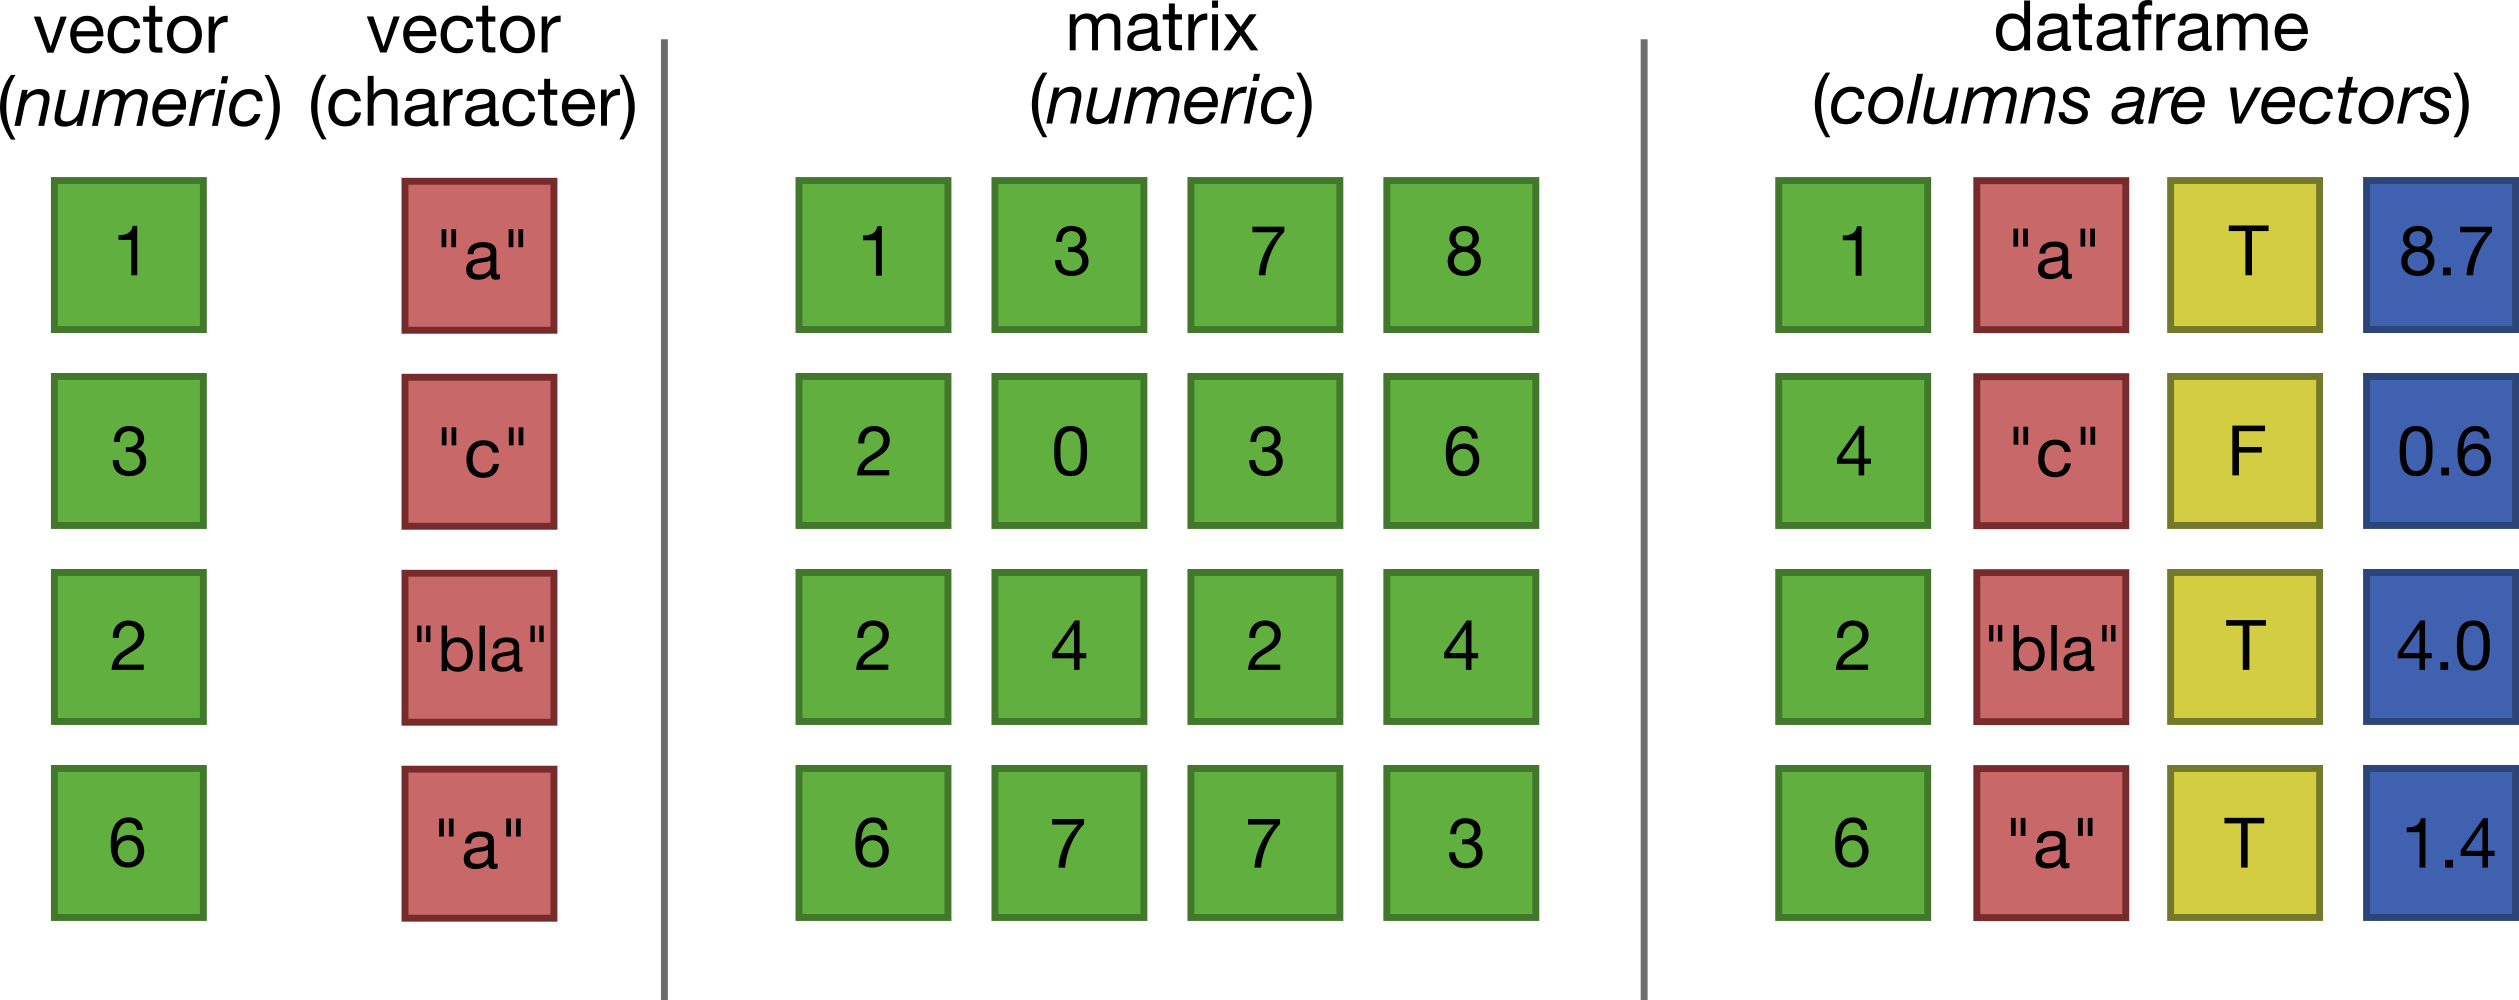
\includegraphics{Programmeren/figuren/datastructs.png}

}

\caption{\label{fig-datastructures}Belangrijkste data structuren in R}

\end{figure}

\hypertarget{sec-vectoren}{%
\subsection{Vectoren}\label{sec-vectoren}}

Om een vector te maken, kunnen we deze handmatig intypen:

\begin{Shaded}
\begin{Highlighting}[]
\NormalTok{mijnvector }\OtherTok{\textless{}{-}} \FunctionTok{c}\NormalTok{(}\DecValTok{1}\NormalTok{,}\DecValTok{2}\NormalTok{,}\FloatTok{0.1}\NormalTok{,}\SpecialCharTok{{-}}\DecValTok{5}\NormalTok{)}
\NormalTok{mijnvector[}\DecValTok{1}\NormalTok{] }\CommentTok{\# geeft het eerste getal}
\NormalTok{mijnvector[}\DecValTok{2}\NormalTok{] }\CommentTok{\# geeft het tweede getal, etc}
\end{Highlighting}
\end{Shaded}

Maar handmatig getallen invoeren is niet altijd handig. Gelukkig kun je
met R een boel lijstjes maken op een snellere manier automatisch
genereren:

\begin{Shaded}
\begin{Highlighting}[]
\DecValTok{1}\SpecialCharTok{:}\DecValTok{4}                \CommentTok{\# 1, 2, 3, 4}
\DecValTok{5}\SpecialCharTok{:}\DecValTok{2}                \CommentTok{\# 5, 4, 3, 2}
\FunctionTok{rep}\NormalTok{(}\DecValTok{2}\NormalTok{,}\DecValTok{4}\NormalTok{)           }\CommentTok{\# 2, 2, 2, 2}
\FunctionTok{seq}\NormalTok{(}\DecValTok{0}\NormalTok{,}\FloatTok{4.5}\NormalTok{,}\FloatTok{1.5}\NormalTok{)     }\CommentTok{\# 0.0, 1.5, 3.0, 4.5}
\FunctionTok{sample}\NormalTok{(}\DecValTok{1}\SpecialCharTok{:}\DecValTok{6}\NormalTok{,}\DecValTok{4}\NormalTok{)      }\CommentTok{\# 4, 6, 3, 5 (iedere keer anders!)}
\FunctionTok{sample}\NormalTok{(letters,}\DecValTok{4}\NormalTok{)  }\CommentTok{\# "f", "j", "o", "y" (iedere keer anders!)}
\FunctionTok{runif}\NormalTok{(}\DecValTok{2}\NormalTok{)           }\CommentTok{\# 0.9965360 0.8978062 (iedere keer anders!)}
\end{Highlighting}
\end{Shaded}

De laatste vijf regels van het bovenstaande script zijn voorbeelden van
``functies''. Een functie is een herhaalbaar blokje code die je aanroept
met de naam (rep, seq, sample), gevolgd door haakjes met daartussen
eventuele \emph{argumenten}. De functie zet deze argumenten om in een
zogeheete \emph{return}-waarde, wat bijvoorbeeld een getal of een lijst
getallen is. Je leert meer over functies in het onderdeel
Paragraaf~\ref{sec-functies}.

Je kan met vectoren ook rekenen. Zo kan je bijvoorbeeld twee vectoren
bij elkaar optellen, of één en hetzelfde getal bij alle elementen van
een vector optellen:

\begin{Shaded}
\begin{Highlighting}[]
\CommentTok{\# Rekenen met vectoren}
\NormalTok{x }\OtherTok{\textless{}{-}} \DecValTok{1}\SpecialCharTok{:}\DecValTok{3}           \CommentTok{\# 1, 2, 3}
\NormalTok{x }\SpecialCharTok{+} \DecValTok{10}             \CommentTok{\# 11 12 13}
\NormalTok{y }\OtherTok{\textless{}{-}} \FunctionTok{c}\NormalTok{(}\DecValTok{1}\NormalTok{, }\DecValTok{10}\NormalTok{, }\DecValTok{4}\NormalTok{)   }\CommentTok{\# 1 10 4}
\NormalTok{x }\SpecialCharTok{+}\NormalTok{ y              }\CommentTok{\# 2 12  7}
\NormalTok{x }\SpecialCharTok{*}\NormalTok{ y              }\CommentTok{\# 1 20 12}
\NormalTok{x }\SpecialCharTok{+}\NormalTok{ y }\SpecialCharTok{/} \DecValTok{100}        \CommentTok{\# 1.01 2.10 3.04}
\NormalTok{(x }\SpecialCharTok{+}\NormalTok{ y) }\SpecialCharTok{/} \DecValTok{100}      \CommentTok{\# 0.02 0.12 0.07}
\end{Highlighting}
\end{Shaded}

In de bovenstaande code zie je een subtiel verschil tussen de laatste
twee regels. Net als bij wiskunde gaan haakjes voor delen en
vermedigvuldigen. Soms moet je dus goed aangeven in welke volgorde je de
berekeninng wil uitvoeren!

\hypertarget{matrices}{%
\subsection{Matrices}\label{matrices}}

Matrices in R kun je maken door de functie \texttt{matrix} aan te
roepen, die je waarden van de matrix en het aantal rijen als argumenten
geeft:

\begin{Shaded}
\begin{Highlighting}[]
\FunctionTok{matrix}\NormalTok{(}\FunctionTok{c}\NormalTok{(}\DecValTok{1}\NormalTok{, }\DecValTok{2}\NormalTok{, }\DecValTok{3}\NormalTok{, }\DecValTok{4}\NormalTok{,}\DecValTok{5}\NormalTok{, }\DecValTok{6}\NormalTok{, }\DecValTok{7}\NormalTok{, }\DecValTok{8}\NormalTok{, }\DecValTok{9}\NormalTok{), }\AttributeTok{nrow=}\DecValTok{3}\NormalTok{)}
\FunctionTok{matrix}\NormalTok{(}\FunctionTok{c}\NormalTok{(}\DecValTok{1}\NormalTok{, }\DecValTok{2}\NormalTok{, }\DecValTok{3}\NormalTok{, }\DecValTok{4}\NormalTok{,}\DecValTok{5}\NormalTok{, }\DecValTok{6}\NormalTok{, }\DecValTok{7}\NormalTok{, }\DecValTok{8}\NormalTok{, }\DecValTok{9}\NormalTok{), }\AttributeTok{nrow=}\DecValTok{3}\NormalTok{, }\AttributeTok{byrow=}\NormalTok{T)}
\end{Highlighting}
\end{Shaded}

Zoals je ziet zijn er geen comments geplaatst bij deze twee regels. Voer
de bovenstaande code zelf uit, en kijk naar de verschillende uitkomsten
van de eerste en de tweede regel. Je kan de matrix ook vullen met andere
waarden:

\begin{Shaded}
\begin{Highlighting}[]
\NormalTok{kansen\_matrix }\OtherTok{\textless{}{-}} \FunctionTok{matrix}\NormalTok{(}\FunctionTok{runif}\NormalTok{(}\DecValTok{9}\NormalTok{),}\AttributeTok{nrow=}\DecValTok{3}\NormalTok{) }\CommentTok{\# willekeurige getallen tussen 0 en 1}
\NormalTok{percentage\_matrix }\OtherTok{\textless{}{-}}\NormalTok{ kansen\_matrix}\SpecialCharTok{*}\DecValTok{100}   \CommentTok{\# de kansen matrix keer 100, dus percentages}
\NormalTok{letter\_matrix }\OtherTok{\textless{}{-}} \FunctionTok{matrix}\NormalTok{(}\FunctionTok{sample}\NormalTok{(letters,}\DecValTok{9}\NormalTok{),}\AttributeTok{nrow=}\DecValTok{3}\NormalTok{) }\CommentTok{\# willekeurige letters}
\end{Highlighting}
\end{Shaded}

\hypertarget{data-frames}{%
\subsection{Data frames}\label{data-frames}}

De laatste (en voor biologen meest belangrijke) data structuur in R is
de data frame. In een dataframe bevat elke kolom een ander gegeven
(naam, leeftijd, haarkleur), en is elke rij een apart observatie. Een
dergelijke structuur is heel handig om wetenschappelijke data te
verzamelen. Ook deze kun je weer handmatig invoeren:

\begin{Shaded}
\begin{Highlighting}[]
\NormalTok{biologen }\OtherTok{\textless{}{-}} \FunctionTok{data.frame}\NormalTok{(}\AttributeTok{naam=}\FunctionTok{c}\NormalTok{(}\StringTok{"Lina"}\NormalTok{,}\StringTok{"Yassin"}\NormalTok{,}\StringTok{"Bram"}\NormalTok{),}
                       \AttributeTok{leeftijd=}\FunctionTok{c}\NormalTok{(}\DecValTok{19}\NormalTok{,}\DecValTok{18}\NormalTok{,}\DecValTok{80}\NormalTok{), }
                       \AttributeTok{haarkleur=}\FunctionTok{c}\NormalTok{(}\StringTok{"Blauw"}\NormalTok{,}\StringTok{"Groen"}\NormalTok{, }\StringTok{"Paars"}\NormalTok{))}
\end{Highlighting}
\end{Shaded}

Als je deze dataset wil bekijken in Rstudio, kun je
\texttt{View(biologen)} typen. Dit opent een tabblad waarin je de data
kan verkennen en sorteren (voor grotere datasets is dit natuurlijk erg
handig!).

Het natuurlijk meestal niet handig om handmatig data frames in te typen
in R. In plaats daarvan kun je grote datasets vaak opslaan of downloaden
in een groot tekstbestand, bijvooreeld in \emph{comma-seperated-value}
(csv) bestanden. Als je een dergelijk tekstbestand hebt, kun je deze
inlezen met de functie \texttt{read.table} of \texttt{read.csv}:

\begin{Shaded}
\begin{Highlighting}[]
\NormalTok{covid\_data }\OtherTok{\textless{}{-}} \FunctionTok{read.csv}\NormalTok{(}\StringTok{"E:/Files/Covid.csv"}\NormalTok{) }\CommentTok{\# waar het bestand staat}
\FunctionTok{head}\NormalTok{(covid\_data) }\CommentTok{\# bekijk de eerste 6 rijen}
\FunctionTok{View}\NormalTok{(covid\_data) }\CommentTok{\# bekijk de hele tabel in Rstudio}
\end{Highlighting}
\end{Shaded}

\hypertarget{indexing}{%
\section{Indexing}\label{indexing}}

Nu je weet hoe je tabellen in kan lezen, is het belangrijk om te leren
over ``indexing''. Indexing is het selecteren van specifieke waarden uit
een vector, matrix, of dataframe. Dit doe je door de positie (index) van
deze elementen tussen vierkante haakjes aan te geven:

\begin{Shaded}
\begin{Highlighting}[]
\NormalTok{jaartallen }\OtherTok{\textless{}{-}} \DecValTok{2009}\SpecialCharTok{:}\DecValTok{2024}         \CommentTok{\# Jaren dat ik biologie "studeer"}
\NormalTok{jaartallen[}\DecValTok{6}\SpecialCharTok{:}\DecValTok{9}\NormalTok{]                 }\CommentTok{\# 2014 2015 2016 2017}

\NormalTok{m }\OtherTok{\textless{}{-}} \FunctionTok{matrix}\NormalTok{(}\FunctionTok{runif}\NormalTok{(}\DecValTok{9}\NormalTok{),}\AttributeTok{nrow=}\DecValTok{3}\NormalTok{)    }\CommentTok{\# Willekeurige getallen in een matrix}
\NormalTok{m[}\DecValTok{1}\NormalTok{,}\DecValTok{2}\NormalTok{]    }\CommentTok{\# rij 1, kolom 2}
\NormalTok{m[}\DecValTok{1}\NormalTok{,]     }\CommentTok{\# rij 1 volledig}
\NormalTok{m[,}\DecValTok{2}\NormalTok{]     }\CommentTok{\# kolom 2 volledig}
\NormalTok{m[}\DecValTok{1}\SpecialCharTok{:}\DecValTok{2}\NormalTok{,}\DecValTok{3}\NormalTok{]  }\CommentTok{\# van rij 1 t/m 2, alleen de 3e kolom}

\NormalTok{biologen }\OtherTok{\textless{}{-}} \FunctionTok{data.frame}\NormalTok{(}\AttributeTok{naam=}\FunctionTok{c}\NormalTok{(}\StringTok{"Lina"}\NormalTok{,}\StringTok{"Yassin"}\NormalTok{,}\StringTok{"Bram"}\NormalTok{),}
                       \AttributeTok{leeftijd=}\FunctionTok{c}\NormalTok{(}\DecValTok{19}\NormalTok{,}\DecValTok{18}\NormalTok{,}\DecValTok{80}\NormalTok{), }
                       \AttributeTok{haarkleur=}\FunctionTok{c}\NormalTok{(}\StringTok{"Blauw"}\NormalTok{,}\StringTok{"Groen"}\NormalTok{, }\StringTok{"Paars"}\NormalTok{))}
\NormalTok{biologen[}\DecValTok{1}\NormalTok{,}\DecValTok{2}\NormalTok{] }\CommentTok{\# eerste rij, tweede kolom (leeftijd: 19)}
\end{Highlighting}
\end{Shaded}

Omdat in data frames de kolommen namen hebben, kun je ook deze gebruiken
om specifieke datapunten te selecteren:

\begin{Shaded}
\begin{Highlighting}[]
\NormalTok{biologen[}\DecValTok{1}\NormalTok{,}\StringTok{"leeftijd"}\NormalTok{] }\CommentTok{\#identiek aan biologen[1,2], maar duidelijker wat je selecteert}
\end{Highlighting}
\end{Shaded}

Je kunt met dataframes ook met het dollar-teken een gehele kolom
opvragen, een kolom bewerken, of een kolom toevoegen:

\begin{Shaded}
\begin{Highlighting}[]
\NormalTok{biologen}\SpecialCharTok{$}\NormalTok{leeftijd}
\NormalTok{biologen}\SpecialCharTok{$}\NormalTok{leeftijd }\OtherTok{\textless{}{-}}\NormalTok{ biologen}\SpecialCharTok{$}\NormalTok{leeftijd }\SpecialCharTok{+} \DecValTok{1}  \CommentTok{\# Alle biolgen zijn 1 jaar ouder geworden}
\NormalTok{biologen}\SpecialCharTok{$}\NormalTok{rol }\OtherTok{\textless{}{-}} \FunctionTok{c}\NormalTok{(}\StringTok{"student"}\NormalTok{,}\StringTok{"assistent"}\NormalTok{,}\StringTok{"docent"}\NormalTok{) }\CommentTok{\# Een nieuwe kolom genaamd \textquotesingle{}rol\textquotesingle{}}
\end{Highlighting}
\end{Shaded}

\hypertarget{selecteren-uit-een-dataframe}{%
\section{Selecteren uit een
dataframe}\label{selecteren-uit-een-dataframe}}

Je kunt condities ook gebruiken op vectoren. Dit geeft dan een vector
van dezelfde lengte, met voor elke positie of aan de conditie voldaan
wordt. Als we bijvoorbeeld de zelf-gemaakte biologen-dataframe nog eens
bekijken, dan kunnen we een vector maken die voor de leeftijd-kolom zegt
wie er jonger is dan 20:

\begin{Shaded}
\begin{Highlighting}[]
\NormalTok{biologen }\OtherTok{\textless{}{-}} \FunctionTok{data.frame}\NormalTok{(}\AttributeTok{naam=}\FunctionTok{c}\NormalTok{(}\StringTok{"Lina"}\NormalTok{,}\StringTok{"Yassin"}\NormalTok{,}\StringTok{"Bram"}\NormalTok{),}
                       \AttributeTok{leeftijd=}\FunctionTok{c}\NormalTok{(}\DecValTok{19}\NormalTok{,}\DecValTok{18}\NormalTok{,}\DecValTok{80}\NormalTok{), }
                       \AttributeTok{haarkleur=}\FunctionTok{c}\NormalTok{(}\StringTok{"Blauw"}\NormalTok{,}\StringTok{"Groen"}\NormalTok{, }\StringTok{"Paars"}\NormalTok{)) }

\NormalTok{jong }\OtherTok{\textless{}{-}}\NormalTok{ biologen}\SpecialCharTok{$}\NormalTok{leeftijd }\SpecialCharTok{\textless{}} \DecValTok{20} \CommentTok{\# geeft TRUE TRUE FALSE}
\end{Highlighting}
\end{Shaded}

Met deze vector kunnen we dan selectie maken uit een dataframe. Weet je
nog dat we hierboven zeiden dat je uit dataframe kan selecteren door
\texttt{{[}rijen,kolommen{]}} aan te geven? Met onze nieuwe
\texttt{jong}-vector, kunnen we dus de juiste rijen pakken:

\begin{Shaded}
\begin{Highlighting}[]
\NormalTok{biologen[jong,] }\CommentTok{\# alleen biologen jonger dan 20}
\end{Highlighting}
\end{Shaded}

Dit is natuurlijk vooral handig als je een grotere dataset hebt, zoals
de bovengenoemde covid-data.

\hypertarget{files-paden-en-de-working-directory}{%
\section{Files, paden, en de `working
directory'}\label{files-paden-en-de-working-directory}}

Om (zoals hierboven) een bestand in te kunnen lezen, moet Rstudio wel
weten waar het bestand staat. Op computers staan alle bestanden in een
hierachische structuur (zie bijvoorbeeld onderstaande Figuur). Hoewel je
misschien gewend bent om door deze structuur van ``mappen'' te klikken
met de muis, moet je in een script altijd precies vertellen waar het
bestand staat. Standaard zoekt Rstudio vaak in de home directory van je
besturingsysteem (\texttt{/Users/Naam} in MacOs,
\texttt{C:/Users/UserName/Documents} in Windows). De directory vanuit
waar Rstudio naar het bestand zoekt, heet de \emph{Working Directory}
(rood omlijnd in de figuur). Door de Working Directory goed in te
stellen, hoef je niet elke keer het hele pad naar het bestand in te
typen (dit heet het absolute pad), maar kun je korter omschrijven waar
het bestand staat (dit heet het relatieve pad). Vaak is het dus handig
om je Working Directory aan te passen naar dezelfde map waar je het
script hebt opgeslagen, zodat je alle data, scripts, en grafieken een
beetje bij elkaar kan houden. Dit kan je doen door, nadat je je script
ergens hebt opgeslagen, te navigeren naar
\texttt{Session\ \textgreater{}\ Set\ Working\ Directory\ \textgreater{}\ To\ Source\ File\ Location}.

\begin{figure}

{\centering 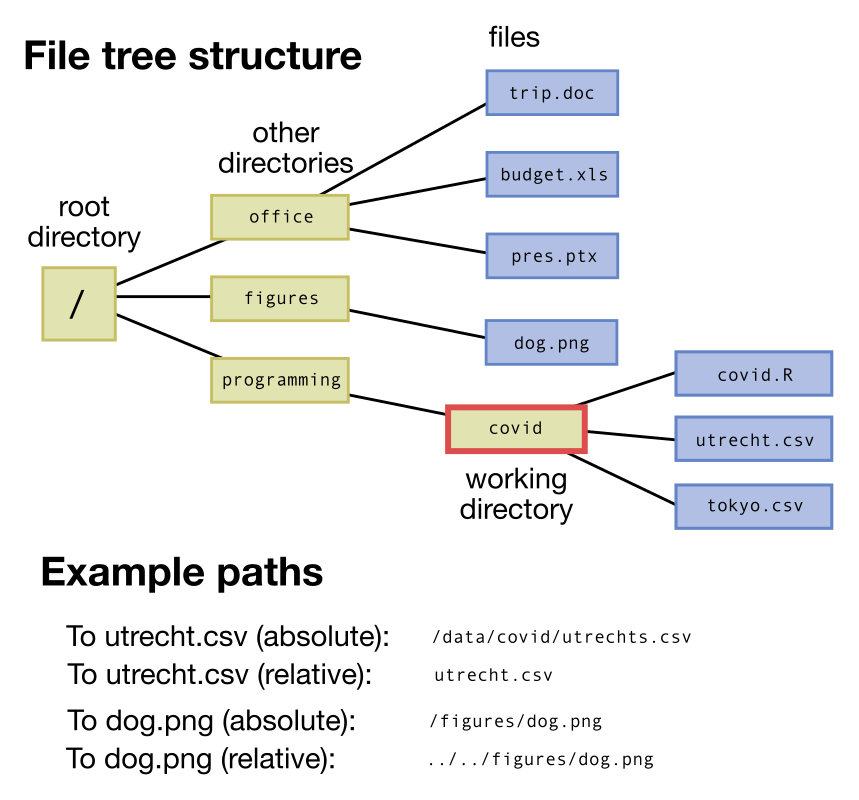
\includegraphics{Programmeren/figuren/file_tree.png}

}

\caption{\label{fig-filesandpaths}Om te programmeren moet je weten waar
bestanden (\emph{files}) staan opgeslagen. Je kunt deze files vinden
door het juiste pad (\emph{paths}) te typens}

\end{figure}

\hypertarget{functies-condities-en-loops}{%
\section{Functies, condities, en
loops}\label{functies-condities-en-loops}}

\hypertarget{sec-functies}{%
\subsection{Functies en help-functie}\label{sec-functies}}

In het onderdeel Paragraaf~\ref{sec-vectoren} heb je al een aantal
voorbeelden gezien van functies, herhaalbare blokjes code die je
gemakkelijk kan aanroepen. Functie hebben een \texttt{input} (waarde(n)
die je meegeeft als zogeheten \emph{argumenten}), en \texttt{output}
(waarde(n) die het terug geeft, de \emph{return}-waarde). Er bestaan
standaard in R een heleboel functies, waarvan je een aantal in deze
cursus nog veel zal tegenkomen:

\begin{itemize}
\tightlist
\item
  \texttt{read.csv}, leest comma-separated-values bestand in als
  dataframe
\item
  \texttt{print} of \texttt{cat}, geeft iets (variabelen of tekst) weer
  in de console
\item
  \texttt{plot}, om data te plotten in een grafiek
\item
  \texttt{length} geeft de lengte van een vector
\item
  \texttt{mean}, gemiddelde van een vector
\item
  \texttt{sd}, standaarddeviatie van een vector
\item
  \texttt{sum}, som van een vector
\item
  \texttt{min} geeft de kleinste waarde in een vector
\item
  \texttt{max} geeft de grootste waarde in een vector
\item
  \texttt{sort}, sorteert een vector
\end{itemize}

Er zijn nog veel meer standaard functies in R. Als je graag meer wil
eten over hoe de functie werkt, kun je de naam van de functie typen met
een \texttt{?} ervoor:

\begin{Shaded}
\begin{Highlighting}[]
\NormalTok{?mean}
\end{Highlighting}
\end{Shaded}

Dit geeft extra uitleg voor deze functie in het ``Help'' venster:

\begin{figure}

{\centering 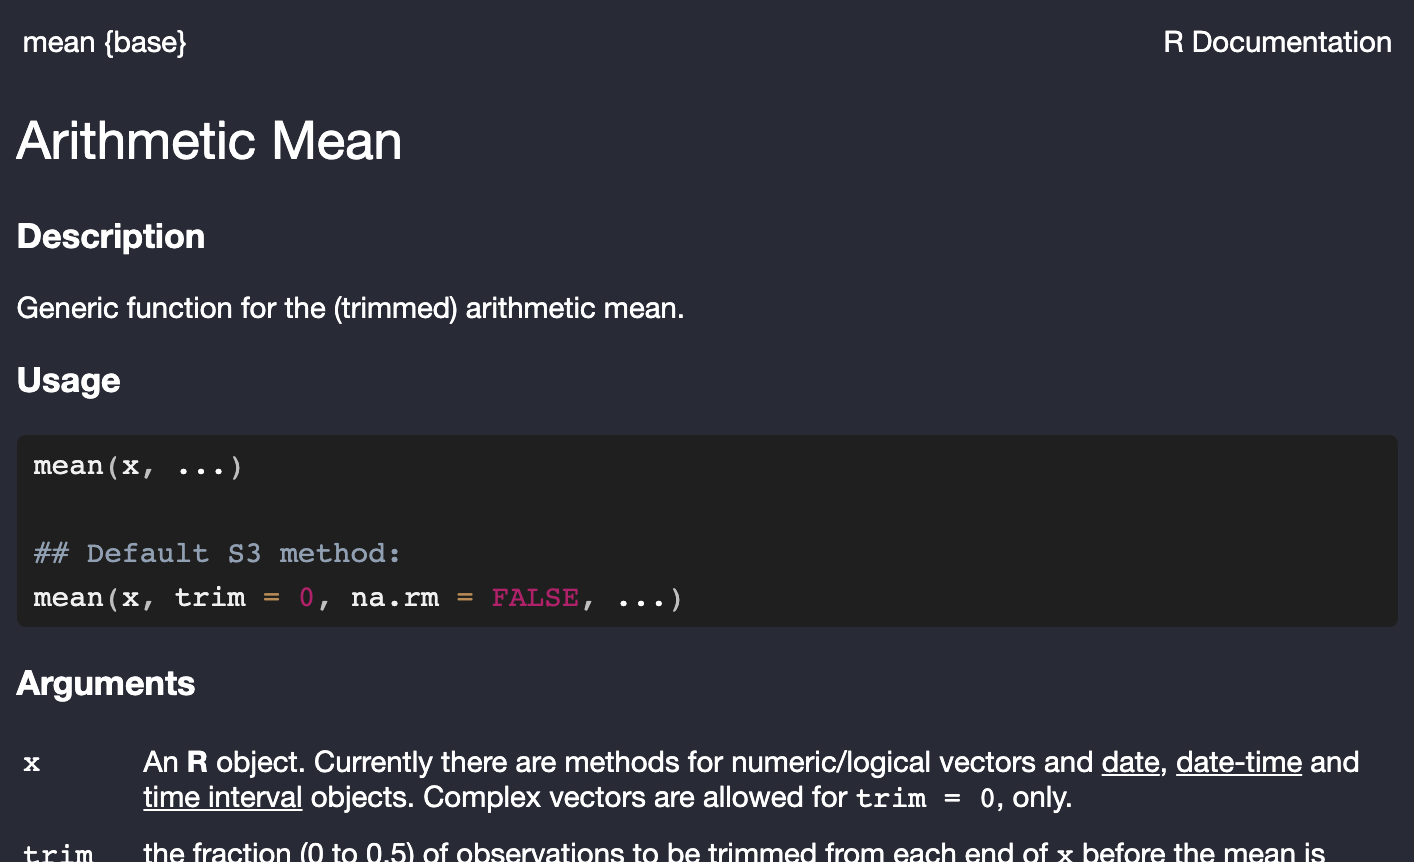
\includegraphics{Programmeren/figuren/Screenshot 2024-07-20 at 17.58.11.png}

}

\caption{\label{fig-helpinR}De help-functie in Rstudie kan je altijd
vertellen wat een bepaalde functie doet, als je \texttt{?functienaam}
typt}

\end{figure}

\hypertarget{zelf-functies-maken}{%
\subsection{Zelf functies maken}\label{zelf-functies-maken}}

Je kan ook zelf functies maken, als je bijvoorbeeld iets heel specifieks
wil doen. Je moet hiervoor aangeven wat de argumenten zijn, welke
berekening op basis van deze argumenten wordt uitgevoerd, en wat er door
de functie wordt teruggegeven (de return-waarde). Hier is een voorbeeld:

\begin{Shaded}
\begin{Highlighting}[]
\CommentTok{\# Definitie van de functie}
\NormalTok{som\_kwadraten }\OtherTok{\textless{}{-}} \ControlFlowTok{function}\NormalTok{(a, b) \{}
\NormalTok{  resultaat }\OtherTok{\textless{}{-}}\NormalTok{ a}\SpecialCharTok{\^{}}\DecValTok{2} \SpecialCharTok{+}\NormalTok{ b}\SpecialCharTok{\^{}}\DecValTok{2}
  \FunctionTok{return}\NormalTok{(resultaat)}
\NormalTok{\}}

\CommentTok{\# Voorbeeld gebruik van de functie}
\FunctionTok{som\_kwadraten}\NormalTok{(}\DecValTok{1}\NormalTok{,}\DecValTok{2}\NormalTok{)            }\CommentTok{\# 5}
\FunctionTok{som\_kwadraten}\NormalTok{(}\DecValTok{3}\NormalTok{, }\DecValTok{4}\NormalTok{)           }\CommentTok{\# 25}
\FunctionTok{som\_kwadraten}\NormalTok{(}\FloatTok{0.5}\NormalTok{, }\FloatTok{0.1}\NormalTok{)       }\CommentTok{\# 0.26}
\end{Highlighting}
\end{Shaded}

Bij het definieren van de functie geven de gekrulde haken aan wat de
zogeheten \texttt{scope} van de functie is: dit blokje code behoort
alleen deze functie toe. Je ziet deze \texttt{scopes} ook terug wanneer
je op bepaalde voorwaarden gaat toetsen, wat het volgende onderdeel zal
uitleggen.

\hypertarget{loops}{%
\section{Loops}\label{loops}}

Hoewel functies het makkelijker maken om dezelfde berekening meerdere
keren uit te voeren, wat nu als je een functie 100 keer wil aanroepen?
Hebben we dan 100 regels nodig? Het antwoord is nee, want elke
programmeertaal (dus ook \texttt{R}) heeft manieren om stukken code
gemakkelijk te herhalen. In R bestaan veel verschillende manieren om dit
te doen (\texttt{repeat}, \texttt{apply}, \texttt{while}), maar in deze
introductie maken we vooral kennis met de meest-gebruikte loop in de
programmeer-wereld: de for-loop.

Laten we bijvoorbeeld de exponentiele afname van paracetamol in het
bloed beschrijven met een simpele ``simulatie'\,'. Iemand neemt 400
milligram paracetamol in, wat ieder uur (ongeveer) met 70\% afneemt:

\begin{Shaded}
\begin{Highlighting}[]
\NormalTok{p }\OtherTok{\textless{}{-}} \DecValTok{400} \CommentTok{\# hoeveelheid paracetamol}
\NormalTok{d }\OtherTok{\textless{}{-}} \FloatTok{0.7} \CommentTok{\# afname (d van decay)}
\CommentTok{\# Herhaal iets 10 keer, waarbij \textquotesingle{}i\textquotesingle{} steeds met 1 toeneemt}
\ControlFlowTok{for}\NormalTok{(i }\ControlFlowTok{in} \DecValTok{1}\SpecialCharTok{:}\DecValTok{10}\NormalTok{)\{}
\NormalTok{  p }\OtherTok{\textless{}{-}}\NormalTok{ p}\SpecialCharTok{*}\NormalTok{d}
\NormalTok{\}}
\FunctionTok{cat}\NormalTok{(}\StringTok{\textquotesingle{}Na 10 uur is er\textquotesingle{}}\NormalTok{,p,}\StringTok{\textquotesingle{}milligram paracetamol in het bloed\textquotesingle{}}\NormalTok{) }\CommentTok{\# 11.299 mg}
\end{Highlighting}
\end{Shaded}

Aan het einde van deze \texttt{for-loop} kunnen we kijken wat de waarde
van p is door in de console \texttt{p} te typen.

\begin{verbatim}
> p
[1] 11.29901
\end{verbatim}

Zoals we eerder hadden besproken, staat de \texttt{{[}1{]}} voor het
feit dat dit de eerste en enige waarde is die in de variable \texttt{p}
is opgeslagen. We hebben nu dus alleen de **laatste* waarde bewaard.
Wellicht willen we echter graag bijhouden hoeveel paracetamol er in elke
stap aanwezig was, zodat we dat na onze loop kunnen plotten. Om dit te
doen, kunnen we de \texttt{i} als index gebruiken om een vector te
vullen:

\begin{Shaded}
\begin{Highlighting}[]
\NormalTok{p }\OtherTok{\textless{}{-}} \DecValTok{400} \CommentTok{\# hoeveelheid paracetamol}
\NormalTok{d }\OtherTok{\textless{}{-}} \FloatTok{0.7} \CommentTok{\# afname (d van decay)}
\CommentTok{\# Herhaal iets 10 keer, waarbij \textquotesingle{}i\textquotesingle{} steeds met 1 toeneemt}
\ControlFlowTok{for}\NormalTok{(i }\ControlFlowTok{in} \DecValTok{1}\SpecialCharTok{:}\DecValTok{10}\NormalTok{)\{}
\NormalTok{  p[i}\SpecialCharTok{+}\DecValTok{1}\NormalTok{] }\OtherTok{\textless{}{-}}\NormalTok{ p[i]}\SpecialCharTok{*}\NormalTok{d}
\NormalTok{\}}
\FunctionTok{plot}\NormalTok{(p, }\AttributeTok{type=}\StringTok{\textquotesingle{}o\textquotesingle{}}\NormalTok{)}
\end{Highlighting}
\end{Shaded}

\begin{figure}[H]

{\centering 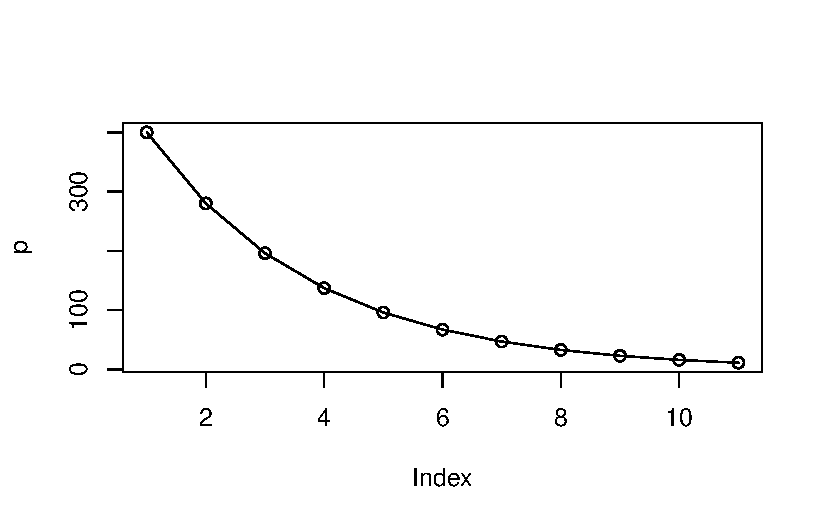
\includegraphics{Programmeren/intro_R_day2_files/figure-pdf/unnamed-chunk-22-1.pdf}

}

\end{figure}

Omdat dit voorbeeld om simpele exponentiele afname gaat, hadden we de
bovenstaande berekening ook ``in één keer'' kunnen uitrekenen door
\(p \cdot d^{10}\) uit te rekenen. Laten we dat even controleren:

\begin{Shaded}
\begin{Highlighting}[]
\NormalTok{p }\OtherTok{\textless{}{-}} \DecValTok{400} \CommentTok{\# hoeveelheid paracetamol}
\NormalTok{d }\OtherTok{\textless{}{-}} \FloatTok{0.7} \CommentTok{\# afname (d van decay)}
\NormalTok{p}\SpecialCharTok{*}\NormalTok{d}\SpecialCharTok{\^{}}\DecValTok{10} \CommentTok{\# 11.299 mg, dat klopt dus!}
\end{Highlighting}
\end{Shaded}

Dit antwoord komt inderdaad overeen met onze berekening met de
\texttt{for} loop. Hoewel deze loop dus misschien wat onnodig lijkt,
hebben we niet altijd zo'n simpele formule beschikbaar. Bovendien willen
we wellicht iets veel specifiekers simuleren, bijvoorbeeld dat de
persoon elke 12 uur opnieuw paracetamol inneemt:

\begin{Shaded}
\begin{Highlighting}[]
\NormalTok{p }\OtherTok{\textless{}{-}} \DecValTok{400} \CommentTok{\# hoeveelheid paracetamol}
\NormalTok{d }\OtherTok{\textless{}{-}} \FloatTok{0.7} \CommentTok{\# afname (d van decay)}

\ControlFlowTok{for}\NormalTok{(i }\ControlFlowTok{in} \DecValTok{1}\SpecialCharTok{:}\DecValTok{100}\NormalTok{)\{}
  \ControlFlowTok{if}\NormalTok{(i}\SpecialCharTok{\%\%}\DecValTok{12}\SpecialCharTok{==}\DecValTok{0}\NormalTok{)\{ }\CommentTok{\# is i precies deelbaar door 12?}
\NormalTok{    p[i] }\OtherTok{\textless{}{-}}\NormalTok{ p[i] }\SpecialCharTok{+} \DecValTok{400}
\NormalTok{  \} }
\NormalTok{  p[i}\SpecialCharTok{+}\DecValTok{1}\NormalTok{] }\OtherTok{\textless{}{-}}\NormalTok{ p[i]}\SpecialCharTok{*}\NormalTok{d}
\NormalTok{\}}
\FunctionTok{plot}\NormalTok{(p, }\AttributeTok{type=}\StringTok{\textquotesingle{}o\textquotesingle{}}\NormalTok{)}
\end{Highlighting}
\end{Shaded}

\begin{figure}[H]

{\centering 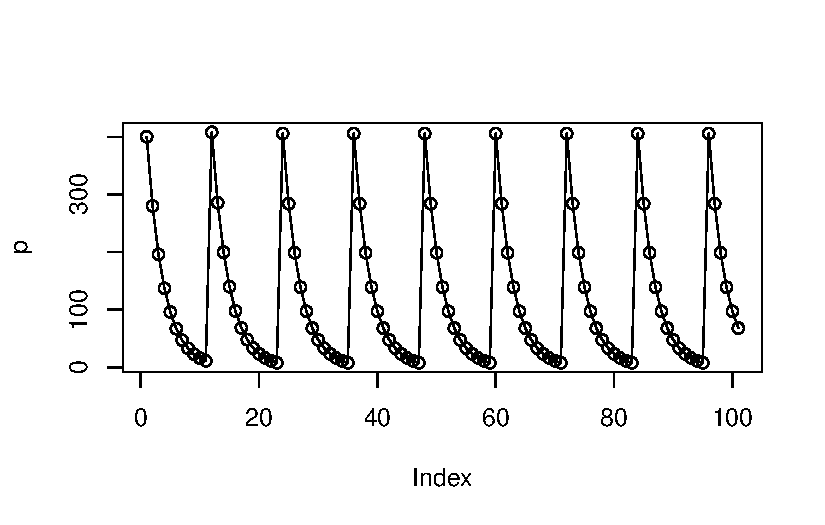
\includegraphics{Programmeren/intro_R_day2_files/figure-pdf/unnamed-chunk-24-1.pdf}

}

\end{figure}

Of dat de persoon met 10\% kans elk uur een paracetamol inneemt:

\begin{Shaded}
\begin{Highlighting}[]
\NormalTok{p }\OtherTok{\textless{}{-}} \DecValTok{400} \CommentTok{\# hoeveelheid paracetamol}
\NormalTok{d }\OtherTok{\textless{}{-}} \FloatTok{0.7} \CommentTok{\# afname (d van decay)}

\ControlFlowTok{for}\NormalTok{(i }\ControlFlowTok{in} \DecValTok{1}\SpecialCharTok{:}\DecValTok{100}\NormalTok{)\{}
  \ControlFlowTok{if}\NormalTok{(}\FunctionTok{runif}\NormalTok{(}\DecValTok{1}\NormalTok{)}\SpecialCharTok{\textless{}}\FloatTok{0.1}\NormalTok{)\{ }\CommentTok{\# is willekeurig getal (tussen 0 en 1) kleiner dan 0.1?}
\NormalTok{    p[i] }\OtherTok{\textless{}{-}}\NormalTok{ p[i] }\SpecialCharTok{+} \DecValTok{400}
\NormalTok{  \} }
\NormalTok{  p[i}\SpecialCharTok{+}\DecValTok{1}\NormalTok{] }\OtherTok{\textless{}{-}}\NormalTok{ p[i]}\SpecialCharTok{*}\NormalTok{d}
\NormalTok{\}}
\FunctionTok{plot}\NormalTok{(p, }\AttributeTok{type=}\StringTok{\textquotesingle{}o\textquotesingle{}}\NormalTok{)}
\end{Highlighting}
\end{Shaded}

\begin{figure}[H]

{\centering 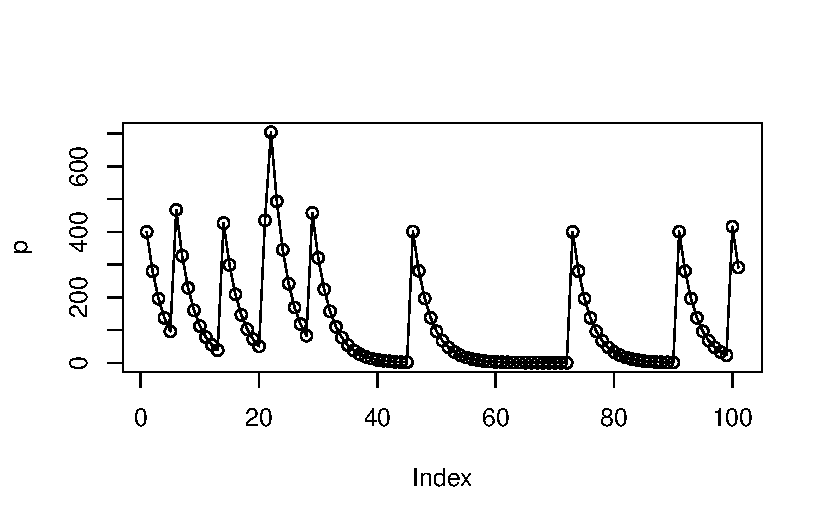
\includegraphics{Programmeren/intro_R_day2_files/figure-pdf/unnamed-chunk-25-1.pdf}

}

\end{figure}

\hypertarget{grafieken-plotten-met-r}{%
\section{Grafieken plotten met R}\label{grafieken-plotten-met-r}}

Om de bovenstaande plot van de paracetamol afname iets vollediger en
mooier te maken, kunnen we meer argumenten aan de plotfunctie toevoegen:

\begin{Shaded}
\begin{Highlighting}[]
\NormalTok{p }\OtherTok{\textless{}{-}} \DecValTok{400} \CommentTok{\# hoeveelheid paracetamol}
\NormalTok{d }\OtherTok{\textless{}{-}} \FloatTok{0.7} \CommentTok{\# afname (d van decay)}

\ControlFlowTok{for}\NormalTok{(i }\ControlFlowTok{in} \DecValTok{1}\SpecialCharTok{:}\DecValTok{100}\NormalTok{)\{}
  \ControlFlowTok{if}\NormalTok{(}\FunctionTok{runif}\NormalTok{(}\DecValTok{1}\NormalTok{)}\SpecialCharTok{\textless{}}\FloatTok{0.1}\NormalTok{)\{ }\CommentTok{\# is willekeurig getal (tussen 0 en 1) kleiner dan 0.1?}
\NormalTok{    p[i] }\OtherTok{\textless{}{-}}\NormalTok{ p[i] }\SpecialCharTok{+} \DecValTok{400}
\NormalTok{  \} }
\NormalTok{  p[i}\SpecialCharTok{+}\DecValTok{1}\NormalTok{] }\OtherTok{\textless{}{-}}\NormalTok{ p[i]}\SpecialCharTok{*}\NormalTok{d}
\NormalTok{\}}
\FunctionTok{plot}\NormalTok{(p, }\AttributeTok{type=}\StringTok{\textquotesingle{}l\textquotesingle{}}\NormalTok{, }\AttributeTok{lwd=}\DecValTok{2}\NormalTok{, }\AttributeTok{col=}\StringTok{"purple"}\NormalTok{, }\AttributeTok{xlab=}\StringTok{"Tijd (uren)"}\NormalTok{, }\AttributeTok{ylab=}\StringTok{"Paracetamol in bloed"}\NormalTok{)}
\FunctionTok{legend}\NormalTok{(}\DecValTok{70}\NormalTok{, }\FunctionTok{max}\NormalTok{(p), }\AttributeTok{legend=}\FunctionTok{c}\NormalTok{(}\StringTok{"Paracetamol"}\NormalTok{), }\AttributeTok{col=}\FunctionTok{c}\NormalTok{(}\StringTok{"purple"}\NormalTok{),}\AttributeTok{lty=}\DecValTok{1}\NormalTok{,}\AttributeTok{lwd=}\DecValTok{2}\NormalTok{)}
\end{Highlighting}
\end{Shaded}

\begin{figure}[H]

{\centering 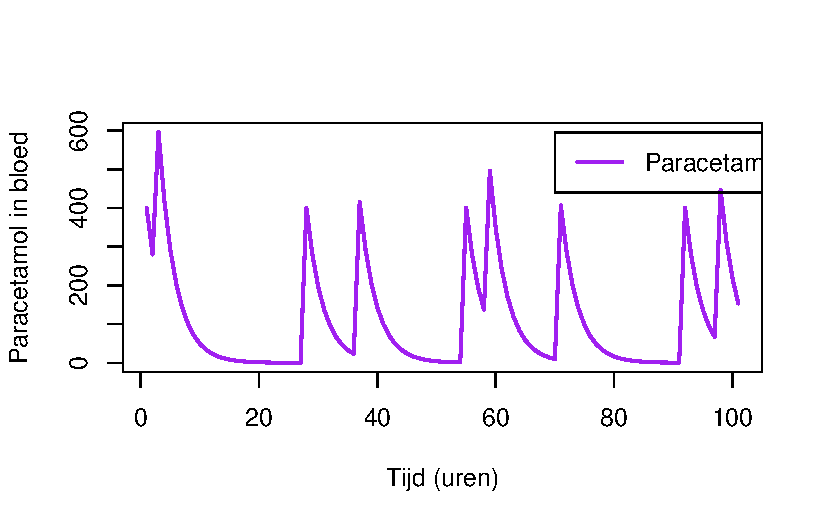
\includegraphics{Programmeren/intro_R_day2_files/figure-pdf/unnamed-chunk-26-1.pdf}

}

\end{figure}

Er zijn binnen R nog veel meer manieren om data te plotten, zoals
bijvoorbeeld de \texttt{boxplot} die je bij het onderdeel statistiek
zeker nog tegen zal komen. Daarnaast zijn er in R veel packages
beschikbaar kunnen helpen bij het maken van mooie grafieken, zoals
\href{https://ggplot2.tidyverse.org/}{ggplot}, maar daar gaan we in deze
cursus niet dieper op in.

\hypertarget{r-oefeningen}{%
\chapter{R oefeningen}\label{r-oefeningen}}

\begin{exercise}[Kennis-vraagjes]\protect\hypertarget{exr-R-1}{}\label{exr-R-1}

\textbf{a.}Wat is het verschil tussen een matrix en een data frame?

\textbf{b.} Als je de code \texttt{x\ \textless{}-\ seq(1,10,by=0.5)}
uitvoert, wat is dan de waarde van \texttt{x{[}2{]}}?

\textbf{c.} Als je de code \texttt{x\ \textless{}-\ 10:1} uitvoert, wat
is dan de waarde van \texttt{x{[}1{]}}?

\textbf{d.} Als je de code \texttt{x\ \textless{}-\ runif(10)} uitvoert,
wat is dan de waarde van \texttt{x{[}1{]}}? En wat geeft
\texttt{x{[}11{]}} dan?

\textbf{e.} Beschouw het volgende data frame:

\begin{Shaded}
\begin{Highlighting}[]
\NormalTok{df }\OtherTok{\textless{}{-}} \FunctionTok{data.frame}\NormalTok{(}\AttributeTok{naam =} \FunctionTok{c}\NormalTok{(}\StringTok{"Jaap"}\NormalTok{, }\StringTok{"Alina"}\NormalTok{, }\StringTok{"Xin"}\NormalTok{),}
                 \AttributeTok{minuten =} \FunctionTok{c}\NormalTok{(}\DecValTok{12}\NormalTok{, }\DecValTok{19}\NormalTok{, }\DecValTok{11}\NormalTok{), }
                 \AttributeTok{score =} \FunctionTok{c}\NormalTok{(}\DecValTok{85}\NormalTok{, }\DecValTok{90}\NormalTok{, }\DecValTok{95}\NormalTok{))}
\end{Highlighting}
\end{Shaded}

Stel we willen een nieuwe kolom toevoegen die de score per minuut geeft,
wat moeten we daarvoor doen?

\textbf{f.} Een student leest de volgende csv in van dieren in het asiel
onder de naam ``dieren'':

\begin{verbatim}
Naam, Leeftijd, Vachtkleur, Temperament
Joey, 8, zwart, rustig
Roos, 2, wit, energiek
Bob, 4, bruin, vriendelijk
Saartje, 2, gevlekt, verlegen
\end{verbatim}

Wat geeft de selectie \texttt{dieren{[}2,3:4{]}} terug?

\textbf{g.} Bekijk de onderstaande for-loop. Wat wordt er na de for-loop
geprint?

\begin{Shaded}
\begin{Highlighting}[]
\NormalTok{a }\OtherTok{\textless{}{-}} \DecValTok{1}
\ControlFlowTok{for}\NormalTok{(i }\ControlFlowTok{in} \DecValTok{1}\SpecialCharTok{:}\DecValTok{3}\NormalTok{)\{}
\NormalTok{  a }\OtherTok{\textless{}{-}}\NormalTok{ a }\SpecialCharTok{+}\NormalTok{ i}
\NormalTok{\}}
\FunctionTok{cat}\NormalTok{(}\StringTok{"De waarde van a is:"}\NormalTok{,a)}
\end{Highlighting}
\end{Shaded}

\end{exercise}

\begin{exercise}[Volgorde]\protect\hypertarget{exr-R-2}{}\label{exr-R-2}

Onder deze tekst staat een stukje code. Neem deze over in Rstudio (tip:
je kan de hele code in 1 keer kopiëren met het knopje rechtsboven).

\begin{Shaded}
\begin{Highlighting}[]
\CommentTok{\# waarden instellen}
\NormalTok{a }\OtherTok{\textless{}{-}} \FloatTok{2.5}
\NormalTok{b }\OtherTok{\textless{}{-}} \DecValTok{11}
\NormalTok{c }\OtherTok{\textless{}{-}} \FloatTok{0.01}

\CommentTok{\# bereken de uitkomst}
\NormalTok{uitkomst }\OtherTok{\textless{}{-}}\NormalTok{ a}\SpecialCharTok{/}\NormalTok{b}\SpecialCharTok{+}\NormalTok{a}\SpecialCharTok{*}\NormalTok{(c}\SpecialCharTok{+}\NormalTok{a)}
\end{Highlighting}
\end{Shaded}

\textbf{a.} Voeg aan het \textbf{einde} van een script een extra regel
toe, waar je de variabele \texttt{a} in \texttt{5} verandert.
\textbf{b.} Voer het script uit. De waarde van de uitkomst-variabele is
niet verandert. Leg met de kook-analogie uit waarom niet.

\end{exercise}

\begin{exercise}[Tabellen inlezen en
plotten]\protect\hypertarget{exr-R-3}{}\label{exr-R-3}

\textbf{a.} Ga naar \url{https://tbb.bio.uu.nl/bvd/bms/}, en klik op
txt-bestand \texttt{covid.txt}. Bekijk de inhoud van dit \textbf{plain
text} bestand. Hoeveel kolommen bevat deze data? Is dit een CSV file?
(hint: zoek op waar CSV voor staat).

\textbf{b.} Bekijk de onderstaande code, en neem deze over. Tel het
aantal rijen met \texttt{nrow}. Zijn dit er 52 zoals in het bestand? Tel
ook het aantal kolommen met \texttt{ncol}. Klopt dit?

\begin{Shaded}
\begin{Highlighting}[]
\CommentTok{\# Lees het bestand covid.txt op de website in met \textquotesingle{}read.table\textquotesingle{}}
\NormalTok{covid }\OtherTok{\textless{}{-}} \FunctionTok{read.csv}\NormalTok{(}\StringTok{"http://tbb.bio.uu.nl/bvd/bms/covid.txt"}\NormalTok{)}
\FunctionTok{View}\NormalTok{(covid)}
\end{Highlighting}
\end{Shaded}

\textbf{c.} Om de kolommen goed in te lezen, kunnen we
\texttt{read.table} gebruiken (deze gaat ervan uit dat de data is
gescheiden door spaties). De onderstaande code gebruikt
\texttt{read.table}. Bekijk nogmaals zorgvuldig de ingelezen tabel Is de
data goed ingelezen?

\begin{Shaded}
\begin{Highlighting}[]
\CommentTok{\# Lees het bestand covid.txt op de website in met \textquotesingle{}read.table\textquotesingle{}}
\NormalTok{covid }\OtherTok{\textless{}{-}} \FunctionTok{read.table}\NormalTok{(}\StringTok{"http://tbb.bio.uu.nl/bvd/bms/covid.txt"}\NormalTok{)}
\end{Highlighting}
\end{Shaded}

\textbf{d.} We passen \texttt{read.table} nog iets verder aan om ervoor
te zorgen dat de eerste rij wordt gezien als de \texttt{header} (de
namen van de kolommen). De data wordt nu goed ingelezen. Bereken hoeveel
positieve testen er gedurende deze periode gemiddeld waren.

\begin{Shaded}
\begin{Highlighting}[]
\CommentTok{\# Lees het bestand covid.txt op de website in met \textquotesingle{}read.table\textquotesingle{} en header=T}
\NormalTok{covid }\OtherTok{\textless{}{-}} \FunctionTok{read.table}\NormalTok{(}\StringTok{"http://tbb.bio.uu.nl/bvd/bms/covid.txt"}\NormalTok{,}\AttributeTok{header=}\NormalTok{T)}
\end{Highlighting}
\end{Shaded}

\textbf{e.} De laatste regel van bovenstaande code gebruikt
\texttt{head} om de eerste 5 regels te van de covid-tabel te laten zien.
Gebruik de hulpfunctie van Rstudio (\texttt{?head}) en pas de code aan
zodat het de eerste 12 rijen van de dataframe laat zien.

\textbf{f.} De functie \texttt{str} kan de structuur van een data frame
samenvatten. Gebruik \texttt{str} om te bepalen hoeveel rijen/kolommen
de covid-dataframe heeft, en welk type variabele er in elke kolom staat.

Om de data beter te kunnen bekijken kunnen we op allerlei manieren
plotten. Laten we het aantal positieve testen over de tijd weergeven.
Hiervoor gebruiken we de functie \texttt{plot()}. Deze functie heeft
veel opties, maar in de basis heeft het alleen twee dingen nodig: een
lijst met getallen voor op de x-as, en een lijst met getallen voor op de
y-as. Zodoende kunnen we gemakkelijk een plotje maken (zie code
hieronder).

\begin{Shaded}
\begin{Highlighting}[]
\CommentTok{\# Lees het bestand covid.txt op de website in met \textquotesingle{}read.table\textquotesingle{}}
\NormalTok{covid }\OtherTok{\textless{}{-}} \FunctionTok{read.table}\NormalTok{(}\StringTok{"http://tbb.bio.uu.nl/bvd/bms/covid.txt"}\NormalTok{,}\AttributeTok{header=}\NormalTok{T)}

\NormalTok{x }\OtherTok{\textless{}{-}}\NormalTok{ covid}\SpecialCharTok{$}\NormalTok{datapunt }\CommentTok{\# alle x{-}punten in een vector}
\NormalTok{y }\OtherTok{\textless{}{-}}\NormalTok{ covid}\SpecialCharTok{$}\NormalTok{positieve\_testen }\CommentTok{\# alle y{-}punten in een vector}
\FunctionTok{plot}\NormalTok{(x,y) }\CommentTok{\# basisplot: alle x{-}punten tegen alle y{-}punten}
\FunctionTok{plot}\NormalTok{(x,y, }\AttributeTok{type=}\StringTok{\textquotesingle{}b\textquotesingle{}}\NormalTok{,}\AttributeTok{lwd=}\DecValTok{2}\NormalTok{,}
     \AttributeTok{xlab=}\StringTok{"Datapunt"}\NormalTok{, }\AttributeTok{ylab=}\StringTok{"Aantal positieve testen"}\NormalTok{,}
     \AttributeTok{col=}\StringTok{"darkblue"}\NormalTok{, }\AttributeTok{main=}\StringTok{"Aantal positieve Covid{-}19 testen in Utrecht"}\NormalTok{) }\CommentTok{\# allerlei extra opties om de plot mooi te maken}

\CommentTok{\# Zoals je hierboven ziet kun je een functie{-}aanroep (hier \textquotesingle{}plot\textquotesingle{})}
\CommentTok{\# ook over meerdere regels verdelen. R weet dat de functie pas \textquotesingle{}af\textquotesingle{} }
\CommentTok{\# is als je het haakje sluit. }
\end{Highlighting}
\end{Shaded}

\textbf{g.} Stel dat we alleen geintresseerd zijn in week 14 t/m 19.
Neem de code hierboven over, en pas deze aan zodat je alleen week 14 t/m
19 plot. Tip: maak een nieuw dataframe genaamd \texttt{covid\_subset}
waarin alleen deze weken voorkomen. Gebruik dan dezelfde plot-functie
als hierboven voor deze dataset. Plot de data ook een keer op een
log-lineaire schaal door \texttt{log="y"} toe te voegen aan de
plot-opties. Wat valt je op?

\textbf{h.} Het zou ook zo kunnen zijn dat je alleen in 2021
geinteresseerd bent. Kijkende naar de data frame zijn dit de eerste 15
rijen, dus deze zouden we kunnen selecteren met
\texttt{covid{[}1:15,{]}}. Met grote tabellen kan het echter handig zijn
om dit automatisch te doen (zie voorbeeld-code hieronder). Pas deze code
aan om alle rijen punten met meer dan 1000 positieve testen te
selecteren. \textbf{Bonus:} voeg de datapunten met meer dan 1000
positieve tesetn toe aan de bestaande grafiek door (na de eerste keer
\texttt{plot()} te gebruiken) de functie \texttt{points()} te gebruiken.
Deze verwacht net als \texttt{plot} een serie x- en y-waarden, maar
voegt deze nu toe aan de bestaande plot.

\begin{Shaded}
\begin{Highlighting}[]
\NormalTok{covid\_subset }\OtherTok{\textless{}{-}}\NormalTok{ covid[covid}\SpecialCharTok{$}\NormalTok{jaar }\SpecialCharTok{==} \DecValTok{2021}\NormalTok{,]}
\NormalTok{x }\OtherTok{\textless{}{-}}\NormalTok{ covid\_subset}\SpecialCharTok{$}\NormalTok{datapunt }\CommentTok{\# alle x{-}punten in een vector}
\NormalTok{y }\OtherTok{\textless{}{-}}\NormalTok{ covid\_subset}\SpecialCharTok{$}\NormalTok{positieve\_testen }\CommentTok{\# alle y{-}punten in een vector}

\FunctionTok{plot}\NormalTok{(x,y, }\AttributeTok{type=}\StringTok{\textquotesingle{}b\textquotesingle{}}\NormalTok{,}\AttributeTok{lwd=}\DecValTok{2}\NormalTok{, }\AttributeTok{log=}\StringTok{"y"}\NormalTok{,}
     \AttributeTok{xlab=}\StringTok{"Datapunt"}\NormalTok{, }\AttributeTok{ylab=}\StringTok{"Aantal positieve testen (log{-}schaal)"}\NormalTok{,}
     \AttributeTok{col=}\StringTok{"darkblue"}\NormalTok{, }\AttributeTok{main=}\StringTok{"Aantal positieve Covid{-}19 testen in Utrecht"}\NormalTok{) }\CommentTok{\# }
\end{Highlighting}
\end{Shaded}

\end{exercise}

\begin{exercise}[Condities en
loops]\protect\hypertarget{exr-R-4}{}\label{exr-R-4}

Je hebt geleerd dat je met een for-loop een bepaalde handeling kan
herhalen. Bekijk de onderstaande for-loop.

\begin{Shaded}
\begin{Highlighting}[]
\ControlFlowTok{for}\NormalTok{(i }\ControlFlowTok{in} \DecValTok{1}\SpecialCharTok{:}\DecValTok{12}\NormalTok{)\{}
\NormalTok{  dobbelsteen }\OtherTok{\textless{}{-}} \FunctionTok{sample}\NormalTok{(}\DecValTok{1}\SpecialCharTok{:}\DecValTok{6}\NormalTok{,}\DecValTok{1}\NormalTok{) }\CommentTok{\# getal van 1 t/m 6 (dobbelsteen worp)}
  \FunctionTok{cat}\NormalTok{(}\FunctionTok{paste}\NormalTok{(}\StringTok{"Worp nummer"}\NormalTok{,i,}\StringTok{"is"}\NormalTok{,dobbelsteen,}\StringTok{"}\SpecialCharTok{\textbackslash{}n}\StringTok{"}\NormalTok{)) }\CommentTok{\#\textbackslash{}n staat voor een \textquotesingle{}enter\textquotesingle{}}
\NormalTok{\}}
\end{Highlighting}
\end{Shaded}

\textbf{a.} De \texttt{cat} functie geeft de gecompileerde zinnetjes
weer in de terminal. Dit wordt in te programmeer-wereld \texttt{printen}
genoemd. Met een dobbelsteen heb je 50\% kans om 4, 5 of 6 te gooien.
Pas de bovenstaande code aan zodat er alleen iets wordt geprint als er
4, 5 of 6 is gegooid. Is het aantal iedere keer precies 50\% van het
aantal progingen? Waaorm wel/niet?

Stel dat we het bovenstaande experiment van 12 keer een dobbelsteen
rollen 100 keer uit willen voeren (honderd replicas). Om dit te doen
kunnen we de bestaande \texttt{for-loop} zelf in een \texttt{for-loop}
zetten. Dit heet het \texttt{nesten} van code. Zo kunnen we bijvoorbeeld
bijhouden hoe vaak we precies 1 keer zes gooien, als we herhaaldelijk 12
keer een dobbelsteen rollen (zie code hieronder)

\begin{Shaded}
\begin{Highlighting}[]
\ControlFlowTok{for}\NormalTok{(e }\ControlFlowTok{in} \DecValTok{1}\SpecialCharTok{:}\DecValTok{100}\NormalTok{)\{}
\NormalTok{  aantal\_keren\_6 }\OtherTok{\textless{}{-}} \DecValTok{0}
  \ControlFlowTok{for}\NormalTok{(i }\ControlFlowTok{in} \DecValTok{1}\SpecialCharTok{:}\DecValTok{12}\NormalTok{)\{}
\NormalTok{    dobbelsteen }\OtherTok{\textless{}{-}} \FunctionTok{sample}\NormalTok{(}\DecValTok{1}\SpecialCharTok{:}\DecValTok{6}\NormalTok{,}\DecValTok{1}\NormalTok{) }\CommentTok{\# getal van 1 t/m 6 (dobbelsteen worp)}
    \ControlFlowTok{if}\NormalTok{(dobbelsteen }\SpecialCharTok{==}\DecValTok{6}\NormalTok{) aantal\_keren\_6 }\OtherTok{\textless{}{-}}\NormalTok{ aantal\_keren\_6 }\SpecialCharTok{+} \DecValTok{1}
\NormalTok{  \}}
\NormalTok{\}}
\end{Highlighting}
\end{Shaded}

\textbf{b.} Pas de bovenstaande code aan, zodat er \textbf{aan het einde
van elk experiment} ``Hoera!'' wordt geprint als er \textbf{precies 1
keer 6 is gegooid}. Kun je de code aanpassen zodat je kan bijhouden hoe
vaak dit is gebeurd?

\end{exercise}

\part{Basiswiskunde}

\hypertarget{sec-algebra}{%
\chapter{Algebra}\label{sec-algebra}}

\hypertarget{introductie}{%
\section{Introductie}\label{introductie}}

Een vergelijking is een wiskundige relatie die één of meerdere onbekende
variabelen bevat. We kunnen erachter komen wat de waarde van deze
onbekende variabele is door de vergelijking op te lossen. Dit hoofdstuk
geeft meer informatie over het oplossen van vergelijkingen.

\hypertarget{volgorde-van-bewerkingen}{%
\section{Volgorde van bewerkingen}\label{volgorde-van-bewerkingen}}

Wiskundige bewerkingen worden altijd in de volgende vaste volgorde
uitgewerkt:

\begin{enumerate}
\def\labelenumi{\arabic{enumi}.}
\item
  haakjes
\item
  machtsverheffen en worteltrekken
\item
  vermenigvuldigen en delen
\item
  optellen en aftrekken
\end{enumerate}

Bewerkingen die op dezelfde plek staan, zijn gelijkwaardig en worden van
links naar rechts uitgevoerd.

\hypertarget{vergelijkingen-met-uxe9uxe9n-onbekende}{%
\section{Vergelijkingen met één
onbekende}\label{vergelijkingen-met-uxe9uxe9n-onbekende}}

In wiskundige vergelijkingen zijn we vaak geinteresseerd in de waarde
van één of meerdere onbekenden. Als we bijvoorbeeld de vergelijking
\(2x = 4\) hebben, willen we graag weten voor welke waarde van \(x\) dit
geldt. Deze vergelijking is zo simpel dat je het misschien meteen ziet:
als \(x\) gelijk is aan \(2\), staat er \(2 \cdot 2\), en klopt de
vergelijking. Maar het is niet altijd eenvoudig om direct af te lezen
welke waarde \(x\) moet hebben om de vergelijking kloppend te maken. Hoe
lossen we bijvoorbeeld de vergelijking \(3x +2 = 7\) of
\(2(x-8) = -10 - x\) op? Allereerst is het belangrijk om te begrijpen
dat deze vergelijkingen \textbf{lineaire verbanden} beschrijven.

\hypertarget{lineaire-verbanden}{%
\subsection{Lineaire verbanden}\label{lineaire-verbanden}}

In een lineaire verband komen geen kwadraten of hogere machten in voor.
We kunnen een lineair verband opschrijven in de algemene vorm
\(y = ax + b\). Hierbij zijn \(x\) en \(y\) de variabelen, en \(a\) en
\(b\) de parameters. De parameter \(a\) zegt iets over hoe snel \(y\)
toeneemt of afneemt als een functie van \(x\). De parameter \(b\)
defineert de beginwaarde, oftewel de waarde van \(y\) als \(x\) gelijk
is aan nul. Deze relatie tussen \(x\) en \(y\) kunnen we nu weergeven in
een assenstelsel:

\begin{figure}

{\centering 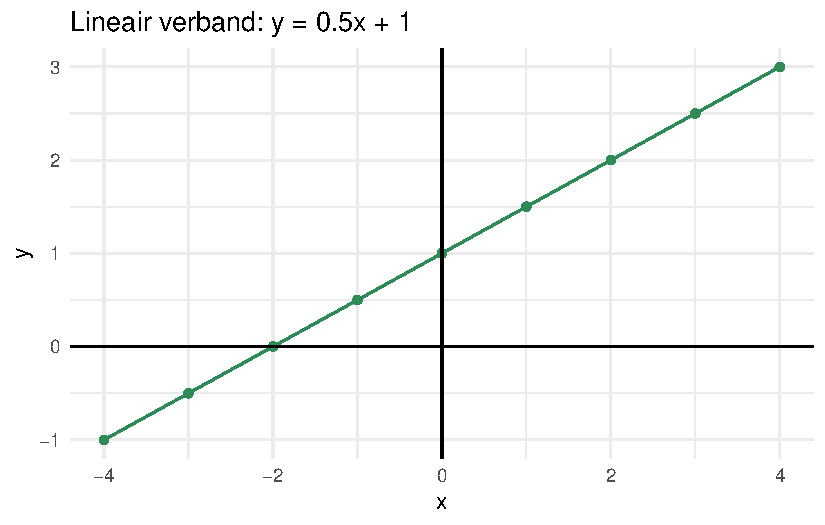
\includegraphics{Wiskunde/algebra_files/figure-pdf/fig-algebra-lineair-1.pdf}

}

\caption{\label{fig-algebra-lineair}Voorbeeld lineair verband.}

\end{figure}

De rechte lijn in de grafiek geeft aan dat we te maken hebben met een
lineair verband.

\hypertarget{vergelijking-oplossen}{%
\subsection{Vergelijking oplossen}\label{vergelijking-oplossen}}

Om vergelijkingen op te lossen maken we gebruik van simpele algebraïsche
handelingen, waarvan de \textbf{balansmethode} de meest belangrijke is:
zo lang je aan beide kanten van het \(=\) teken dezelfde bewerkingen
doet, blijft de vergelijking altijd gelden. Als je aan beide kanten van
het \(=\) teken dezelfde hoeveelheid optelt, aftrekt, of met dezelfde
hoeveelheid vermenigvuldigt, is er feitelijk niets veranderd. Om
lineaire vergelijkingen op te lossen kun je gebruik maken van het
volgende stappenplan:

\begin{figure}

\begin{minipage}[t]{0.45\linewidth}

{\centering 

\textbf{Stappenplan lineaire vergelijkingen:}

\begin{enumerate}
\def\labelenumi{\arabic{enumi}.}
\item
  Haakjes uitwerken.
\item
  Alles met de variabele naar links.
\item
  Alles zonder de variabele naar rechts.
\item
  Delen door het getal voor de variabele.
\end{enumerate}

}

\end{minipage}%
%
\begin{minipage}[t]{0.55\linewidth}

{\centering 

\textbf{Voorbeeld:} \(2(x-8) = - 10 - x\)

\begin{enumerate}
\def\labelenumi{\arabic{enumi}.}
\item
  \(2x-16 = - 10 - x\)
\item
  Aan beide kanten x optellen: \(3x-16 = - 10\)
\item
  Aan beide kanten 16 aftrekken: \(3x = 6\)
\item
  Aan beide kanten delen door 3: \(x = 6/3 \rightarrow x = 2\)
\end{enumerate}

}

\end{minipage}%

\end{figure}

\hypertarget{kwadratische-verbanden}{%
\subsection{Kwadratische verbanden}\label{kwadratische-verbanden}}

Een kwadratisch, of tweedegraads, verband heeft de vorm
\(y = ax^2 + bx + c\).

\begin{figure}

{\centering 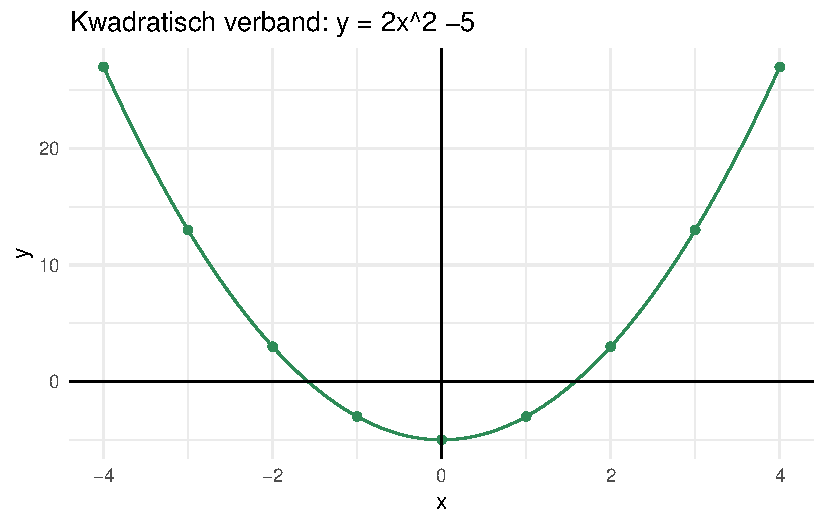
\includegraphics{Wiskunde/algebra_files/figure-pdf/fig-algebra-kwadratisch-1.pdf}

}

\caption{\label{fig-algebra-kwadratisch}Voorbeeld kwadratisch verband.}

\end{figure}

Het oplossen van een kwadratische vergelijking kan op verschillende
manieren. Stel allereerst je voor dat \(c = 0\). In dit geval bevatten
alle termen \(x\), en kunnen we \(x\) buiten haakjes halen. Je krijgt
dan twee oplossingen, waarvan er altijd één is waarbij \(x=0\). Bekijk
bijvoorbeeld hetvolgende voorbeeld:

\begin{figure}

\begin{minipage}[t]{0.45\linewidth}

{\centering 

\textbf{Stappenplan kwadratische vergelijkingen:}

\begin{enumerate}
\def\labelenumi{\arabic{enumi}.}
\item
  Haakjes uitwerken.
\item
  Alles met de variabele naar links.
\item
  Alles zonder de variabele naar rechts.
\item
  Delen door het getal voor de variabele.
\end{enumerate}

}

\end{minipage}%
%
\begin{minipage}[t]{0.55\linewidth}

{\centering 

\textbf{Voorbeeld:} \(2x^2 + 4x = 0\)

\begin{enumerate}
\def\labelenumi{\arabic{enumi}.}
\item
  \(x(2x+4) = 0\)
\item
  \(x(2x+4)\) is gelijk aan 0, als:

  \begin{enumerate}
  \def\labelenumii{\arabic{enumii}.}
  \item
    \[ x = 0 \]

    OF
  \item
    \[2x+4 = 0\] \[2x = -4\] \[x = -4/2\] \[x = -2\]
  \end{enumerate}
\end{enumerate}

}

\end{minipage}%

\end{figure}

Als \(c\) echter niet gelijk is aan \(0\), is er een derde term die
\emph{geen} \(x\) bevat. Het oplossen van kwadratische vergelijkingen
waarbij er een term is die geen \(x\) bevat kan niet opgelost worden
door \(x\) buiten haakjes te halen. Dit is het geval voor vergelijkingen
met de vorm \(y = ax^2 + bx + c\) (waarbij \(c \neq 0\)). Hiervoor
kunnen we de abc-formule gebruiken. Deze formule geeft de twee mogelijke
oplossingen: \(x_{1} = \frac{-b + \sqrt{b^2 - 4ac}}{2a}\) en
\(x_{2} = \frac{-b - \sqrt{b^2 - 4ac}}{2a}\).

\hypertarget{opdrachten}{%
\section{Opdrachten}\label{opdrachten}}

\begin{exercise}[]\protect\hypertarget{exr-algebra-1}{}\label{exr-algebra-1}

Los de volgende vergelijkingen op:

\textbf{a.}

\(3x + 5 = 11\)

\textbf{b.}

\(x^2 + 2x - 8 = 0\)

\textbf{c.}

\(x^2 - 9 = 0\)

\end{exercise}

\begin{exercise}[]\protect\hypertarget{exr-algebra-2}{}\label{exr-algebra-2}

Vereenvoudig de volgende uitdrukking:

\((ax-2by)(3y-4bx)+2b(2ax^2+3y^2)-8xyb^2\)

\end{exercise}

\begin{exercise}[]\protect\hypertarget{exr-algebra-3}{}\label{exr-algebra-3}

Los de vergelijkingen op voor de aangegeven variabele (geef je antwoord
in de vorm variabele = \ldots):

\textbf{a.} vind \(r\) in: \(3r + 2 - 5(r+1) = 6r+4\)

\textbf{b.} vind \(x\) in: \(x + {4 \over x} =4\)

\textbf{c.} vind \(N\) in: \((b-{N \over k})N=0\)

\textbf{d.} vind \(N\) in:
\((b-d(1+{N \over k}))N=0,\;\;d \ne 0;\;k \ne 0\)

\textbf{e.} vind \(N\) in: \((\frac{b}{1+N/h}-d)N=0, \;b \ne 0\)

\end{exercise}

\hypertarget{sec-breuken}{%
\chapter{Breuken}\label{sec-breuken}}

\hypertarget{introductie-1}{%
\section{Introductie}\label{introductie-1}}

Veel biologische processen worden wiskundig beschreven met
vergelijkingen waarin breuken voorkomen. Dit hoofdstuk beschrijft de
belangrijkste rekenregels voor het werken met breuken, zodat je goed
voorbereid bent om dit soort modellen aan de slag te gaan.

\hypertarget{rekenregels-voor-breuken}{%
\section{Rekenregels voor breuken}\label{rekenregels-voor-breuken}}

Een breuk bestaat altijd uit een \textbf{teller} (\emph{numerator} in
het Engels) en een \textbf{noemer} (\emph{denominator} in het Engels).
In de breuk \(\frac{a}{b}\), is a de teller is en b de noemer.

\hypertarget{vereenvoudigen}{%
\subsection*{Vereenvoudigen}\label{vereenvoudigen}}
\addcontentsline{toc}{subsection}{Vereenvoudigen}

Als een breuk zowel boven als onder de deelstreep wordt vermenigvuldigd
met hetzelfde getal mag dit getal weggestreept worden. \[
\frac{ca}{cb} = \frac{a}{b}
\] Hetzelfde geldt als zowel de teller als de noemer door hetzelfde
getal gedeeld wordt. \[
\frac{a/c}{b/c} = \frac{a}{b}
\] Deze rekenregel verklaart ook dat bijvoorbeeld \(\frac{4}{8}\)
vereenvoudigd mag worden tot \(\frac{1}{2}\)
(\(\frac{4}{8} = \frac{4\cdot1}{4\cdot2} = \frac{1}{2}\)).

\hypertarget{vermenigvuldigen}{%
\subsection*{Vermenigvuldigen}\label{vermenigvuldigen}}
\addcontentsline{toc}{subsection}{Vermenigvuldigen}

Het vermenigvuldigen van twee breuken gaat volgens de regel ``teller
keer teller, noemer keer noemer''.

\[
\frac{a}{b}\cdot\frac{c}{d}=\frac{ac}{bd}
\]

\begin{tcolorbox}[enhanced jigsaw, coltitle=black, breakable, bottomtitle=1mm, opacityback=0, colback=white, rightrule=.15mm, title=\textcolor{quarto-callout-tip-color}{\faLightbulb}\hspace{0.5em}{Tip}, bottomrule=.15mm, toprule=.15mm, left=2mm, colframe=quarto-callout-tip-color-frame, toptitle=1mm, opacitybacktitle=0.6, titlerule=0mm, colbacktitle=quarto-callout-tip-color!10!white, leftrule=.75mm, arc=.35mm]

Deze regel kun je ook gebruiken als je een breuk vermenigvuldigt met een
geheel getal. Het gehele getal kun je schrijven als een breuk met als
noemer 1. Bijvoorbeeld:

\[
5\cdot\frac{2}{7} = \frac{5}{1}\cdot\frac{2}{7} = \frac{5\cdot2}{1\cdot7} = \frac{10}{7}
\]

\end{tcolorbox}

\hypertarget{delen}{%
\subsection*{Delen}\label{delen}}
\addcontentsline{toc}{subsection}{Delen}

De vuistregel bij het delen door een breuk is: ``delen door een breuk is
vermenigvuldigen met het omgekeerde''. Dit geldt zowel bij het delen van
gehele getallen als bij het delen van breuken.

\[
a\div \frac{b}{c} = a\cdot\frac{c}{b} = \frac{ac}{b}
\] \[
\frac{a}{b}\div\frac{c}{d} = \frac{a}{b}\cdot\frac{d}{c} = \frac{ad}{bc}
\]

\hypertarget{optellen-en-aftrekken}{%
\subsection*{Optellen en aftrekken}\label{optellen-en-aftrekken}}
\addcontentsline{toc}{subsection}{Optellen en aftrekken}

Breuken kunnen alleen bij elkaar worden opgeteld als ze gelijknamig zijn
(dezelfde noemer hebben).

\[
\frac{a}{b}+\frac{c}{b} = \frac{a+c}{b}
\]

Maar hoe los je bijvoorbeeld het volgende probleem op? \[
\frac{a}{b}+\frac{c}{d} 
\]

Als breuken niet gelijknamig zijn, moeten ze eerst gelijknamig gemaakt
worden voordat ze opgeteld kunnen worden. Dit kun je doen door de teller
en noemer van de eerste breuk te vermenigvuldigen met de noemer van de
tweede breuk, en op dezelfde manier de teller en noemer van de tweede
breuk te vermenigvuldigen met de noemer van de eerste breuk.

Dit mag omdat een breuk waarbij de teller en noemer gelijk zijn, altijd
1 is (\(\frac{d}{d}=1\)). Als je een getal vermenigvuldigt met 1
verandert de waarde van het getal niet, je mag dit dus altijd doen. \[
\frac{a}{b} = \frac{a}{b}\cdot\frac{d}{d} = \frac{ad}{bd}
\] \[
\frac{c}{d} = \frac{c}{d}\cdot\frac{b}{b} = \frac{bc}{bd}
\]

Zoals je ziet, zijn beide breuken nu gelijknamig en mogen we ze dus
optellen. Dit doen we door de tellers bij elkaar op te tellen, terwijl
de noemer hetzelfde blijft.

\[
\frac{a}{b}+\frac{c}{d} = \frac{ad}{bd}+\frac{bc}{bd} = \frac{ad + bc}{bd}
\]

Dezelfde regels gelden voor het aftrekken van breuken: als de breuken
gelijknamig zijn mag je de tellers van elkaar aftrekken. Zijn ze niet
gelijknamig? Dan moet je ze eerst gelijknamig maken zoals hierboven
beschreven.

\hypertarget{breuken-uit-een-vergelijking-halen}{%
\subsection*{Breuken uit een vergelijking
halen}\label{breuken-uit-een-vergelijking-halen}}
\addcontentsline{toc}{subsection}{Breuken uit een vergelijking halen}

Soms kan het handig zijn om een vergelijking met een breuk erin om te
schrijven, zodat de breuk verdwijnt. Dit kun je doen door de
vergelijking aan de rechter- en linkerkant van het = teken te
vermenigvuldigen met de noemer van de breuk. Doordat je beide kanten van
het is-teken vermenigvuldigt met hetzelfde getal, blijft de vergelijking
kloppend.

\[
\frac{a}{b} = cx
\] \[
a = bcx
\]

\hypertarget{voorbeelden}{%
\subsection*{Voorbeelden}\label{voorbeelden}}
\addcontentsline{toc}{subsection}{Voorbeelden}

\subsubsection{Voorbeelden}

Probeer eerst zelf de vergelijkingen op te lossen voordat je naar de
uitleg kijkt!

\subsubsection{\texorpdfstring{Los op:
\(\frac{2}{5x}+\frac{3}{4} = 0.5\)}{Los op: \textbackslash frac\{2\}\{5x\}+\textbackslash frac\{3\}\{4\} = 0.5}}

\emph{Los de volgende vergelijking op:}
\(\frac{2}{5x}+\frac{3}{4} = 0.5\).

Dit kan op twee verschillende manieren. De eerste manier is het meest
eenvoudig, maar voor de volledigheid staat manier twee ook in de uitleg.

\begin{enumerate}
\def\labelenumi{\arabic{enumi}.}
\item
  Eerst de breuken optellen. Om dit te doen moeten de breuken eerst
  dezelfde noemer hebben:
  \(\frac{2\cdot4}{5x\cdot4} + \frac{3\cdot5x}{4\cdot5x} = 0.5\) oftewel
  \(\frac{8}{20x} + \frac{15x}{20x} = 0.5\). Nu kunnen we de breuken
  optellen: \(\frac{8+15x}{20x} = 0.5\). Daarna kunnen we de breuk
  weghalen door aan beide kanten te vermenigvuldigen met \(20x\), dan
  krijgen we: \(8+15x = 10x\). Door aan beide kanten \(15x\) af te
  trekken krijgen we \(8 = -5x\) oftwel \(x = -\frac{8}{5}\).
\item
  Meteen de breuk met x isoleren door aan beide kanten \(\frac{3}{4}\)
  af te trekken: \(\frac{2}{5x} = 0.5-\frac{3}{4}\). We kunnen \(0.5\)
  vervolgens als een breuk schrijven om de twee getallen aan de
  rechterkant van elkaar af te trekken:
  \(\frac{2}{5x} = \frac{1}{2}-\frac{3}{4}\). Gelijknamig maken van deze
  breuken geeft:
  \(\frac{2}{5x} = \frac{1\cdot4}{2\cdot4}-\frac{3\cdot2}{4\cdot2}\)
  oftewel \(\frac{2}{5x} = \frac{4}{8}-\frac{6}{8}\). Nu kunnen we de
  breuken van elkaar aftrekken: \(\frac{2}{5x} = -\frac{2}{8}\). In zo'n
  situatie, waarbij er aan beide kanten van het is-teken enkel een breuk
  staat, mag je de noemer van de eerste breuk vermenigvuldigen met de
  teller van de andere breuk, en vice versa: \(2 = -\frac{2\cdot5x}{8}\)
  en \(2\cdot8 = -2\cdot5x\). Dit geeft \(16 = - 10x\). Dus
  \(x = -\frac{16}{10}\), en vereenvoudigd \(x = -\frac{8}{5}\).
\end{enumerate}

\subsubsection{\texorpdfstring{Los op:
\(\frac{2}{x+3}=5\)}{Los op: \textbackslash frac\{2\}\{x+3\}=5}}

\emph{Los de volgende vergelijking op:} \(\frac{2}{x+3}=5\).

Door aan beide kanten met \(x+3\) te vermenigvuldigen verwijderen we de
breuk \(2 = 5(x+3)\). Haakjes uitwerken geeft \(2 = 5x + 15\). We kunnen
de term met \(x\) erin isoleren door aan beide kanten van het is-teken
\(15\) af te trekken. Dit geeft: \(2-15 = 5x\) oftewel \(-13 = 5x\).
Delen door \(5\) geeft: \(x = -\frac{13}{5}\).

\hypertarget{opdrachten-1}{%
\section{Opdrachten}\label{opdrachten-1}}

\begin{exercise}[]\protect\hypertarget{exr-breuken-1}{}\label{exr-breuken-1}

Reken uit, en vereenvoudig waar mogelijk:

\textbf{a.} \(\frac{1}{7}\cdot\frac{2}{4}\)

\textbf{b.} \(\frac{1}{6}-\frac{2}{3}\)

\textbf{c.} \(\frac{2}{3}\div\frac{4}{5}\)

\textbf{d.} \(\frac{4}{12}+\frac{5}{36}\)

\end{exercise}

\begin{exercise}[]\protect\hypertarget{exr-breuken-2}{}\label{exr-breuken-2}

Familie Jansen heeft een inkomen van 2400 euro. Ze besteden
\(\frac{1}{3}\) van het inkomen aan hun hypotheek, \(\frac{1}{7}\) aan
boodschappen en \(\frac{1}{4}\) aan gas, water en elektriciteit. Ze
krijgen \(\frac{1}{3}\) van hun hypotheekbetalingen terug van de
belastingdienst. Hoe veel geld houdt familie Jansen elke maand over?
Reken uit door alle breuken eerst samen te voegen in één breuk.

\end{exercise}

\begin{exercise}[]\protect\hypertarget{exr-breuken-3}{}\label{exr-breuken-3}

Schrijf als één breuk:

\(\frac{6}{r} - \frac{5r}{30r+5}\)

\end{exercise}

\begin{exercise}[]\protect\hypertarget{exr-breuken-4}{}\label{exr-breuken-4}

Los op voor x:

\(\frac{a}{b}x - \frac{c}{d} = \frac{e}{f}\)

\end{exercise}

\begin{exercise}[]\protect\hypertarget{exr-breuken-5}{}\label{exr-breuken-5}

Los op voor A:

\(25A\div\frac{3}{7} = 12 - \frac{1}{3}A\)

\end{exercise}

\begin{exercise}[]\protect\hypertarget{exr-breuken-6}{}\label{exr-breuken-6}

Los op voor N:

\textbf{a.} \((b-\frac{N}{k})N = 0\)

\textbf{b.} \((b-d(1+\frac{N}{k}))N = 0\) waarbij \(d\neq0; k\neq0\)

\textbf{c.} \((\frac{b}{1+N/h}-d)N = 0\) waarbij \(b\neq0\)

\end{exercise}

\hypertarget{sec-exponenten}{%
\chapter{Exponenten \& Logaritmen}\label{sec-exponenten}}

\hypertarget{introductie-2}{%
\section{Introductie}\label{introductie-2}}

Stel je één enkele bacterie voor op een agarplaat. Deze bacteriesoort
groeit snel en deelt zich elk uur. Na één uur zijn er \(1 \cdot 2 = 2\)
bacteriën. Na vijf uur zijn dat er
\(1 \cdot 2 \cdot 2 \cdot 2 \cdot 2 \cdot 2 = 32\). Gelukkig is er een
makkelijke manier om dit op te schrijven: na \(n\) delingen, zijn er
\(2^n\) bacteriën. Dit is een simpel voorbeeld van exponentiële groei,
die we ook kunnen uitdrukken met de volgende vergelijking, waarbij \(B\)
het aantal bacteriën is en \(n\) het aantal delingen:
\begin{equation}\protect\hypertarget{eq-bact-groei}{}{
B = B_0\cdot2^n
}\label{eq-bact-groei}\end{equation} Hierbij staat \(B_0\) voor het
aantal bacteriën waarmee je start. Hoewel je misschien gewend bent dat
wiskundige functies vaak in de vorm \(y=f(x)\) geschreven worden, kun je
\(y\) en \(x\) vervangen met letters die voor de biologie wat logischer
zijn: \(B\) voor \textbf{b}acteriën, en \(n\) voor \emph{\textbf{n}umber
of divisions.} Exponententen en logaritmen (het omgekeerde van een
exponent) komen veel voor in biologische processen, dus het is
belangrijk om er mee te leren rekenen. In dit onderdeel bespreken we
daarom de relevante rekenregels.

\hypertarget{exponenten}{%
\section{Exponenten}\label{exponenten}}

Een exponent geeft aan hoe vaak het grondtal met zichzelf
vermenigvuldigd wordt.\\
Bijvoorbeeld \(2^4 = 2 \cdot 2 \cdot 2 \cdot 2 = 16\). Hierbij is 2 het
grondtal en 4 de exponent.\\
Wortels kunnen ook als exponent weergegeven worden, de exponent is dan
gelijk aan \(1\over2\).\\
Bijvoorbeeld \(\sqrt{4} = 4^{1\over2} = 2\).

\begin{longtable}[]{@{}
  >{\raggedright\arraybackslash}p{(\columnwidth - 2\tabcolsep) * \real{0.5417}}
  >{\raggedright\arraybackslash}p{(\columnwidth - 2\tabcolsep) * \real{0.4583}}@{}}
\toprule\noalign{}
\begin{minipage}[b]{\linewidth}\raggedright
Rekenregel
\end{minipage} & \begin{minipage}[b]{\linewidth}\raggedright
Voorbeeld
\end{minipage} \\
\midrule\noalign{}
\endhead
\bottomrule\noalign{}
\endlastfoot
\(a^n \cdot a^m = a^{n + m}\) & \(2^2 \cdot 2^3 = 2^{2+3} = 2^5\) \\
\(a^n \div a^m = a^{n - m}\) als \(a \neq 0\) &
\(2^5 \div 2^2 = 2^{5-2} = 2^3\) \\
\((a^n)^m = a^{nm}\) & \((2^2)^2 = 2^4\) \\
\((a^n \cdot b^m)^q = a^{nq} \cdot b^{mq}\) &
\((2^3 \cdot 3^4)^2 = 2^6 \cdot 3^8\) \\
\(a^{-n} = 1 / a^n\) & \(4^{-2} = 1/4^2\) \\
\(a^0 = 1\) & \(2^0 = 1\) \\
\end{longtable}

\hypertarget{hele-grote-en-hele-kleine-getallen}{%
\subsection{Hele grote en hele kleine
getallen}\label{hele-grote-en-hele-kleine-getallen}}

In de biologie werken we vaak met grote waardes, zoals megatonnen
uitgestoten \(CO_2\) of miljoenen rode bloedcellen geproduceerd per uur.
Deze grote waarden worden meestal aangegeven met een macht van tien. Zo
kan \(2500\) opgeschreven worden als \(2.5 \cdot 1000 = 2.5\cdot10^3\) .
Ook erg kleine getallen kunnen zo opgeschreven worden:
\(0.000015 = 1.5 \cdot 0.00001 = 1.5\cdot10^{-5}\) Een andere manier om
dit op te schrijven is: \(1.5 \cdot 10^{-5} = 1.5E − 5 = 1.5 \exp −5\)
en \(2.5 \cdot 10^3 = 2.5 E3=2.5e3\). Zulke notaties zul je voornamelijk
terugvinden in grafieken.

\hypertarget{logaritmen}{%
\section{Logaritmen}\label{logaritmen}}

De logaritme is het omgekeerde van de exponent. Je kunt een exponent
altijd herschrijven als een logaritme, en andersom: \(^2\log{16} = 4\)
want \(2^4 = 16\). Dit is belangrijk, omdat het kan zijn dat de
onbekende die je wil oplossen de exponent is, bijvoorbeeld \(2^x = 18\).
Hier staat dus eigenlijk: tot welke macht moeten we \(2\) verheffen, om
\(18\) te krijgen. Om dit op te lossen, schrijven we om naar een
logaritme: \(x=^2\log{18}\).\\
\strut \\
Meer algemeen kunnen we zeggen: als \(^a\log{c}=b\) dan geldt \(a^b=c\).
Hierbij is \(a\) het grontal en \(b\) de exponent. Als het grontal van
de logaritme weg is gelaten, dan is het grondtal 10
(\(\log{c} = ^{10}\log{c}\)). Een logaritme met grondtal \(e\) heet de
natuurlijke logaritme (ln), en wordt zo geschreven:
\(^e\log{c} = \ln{c}\)

\begin{longtable}[]{@{}
  >{\raggedright\arraybackslash}p{(\columnwidth - 2\tabcolsep) * \real{0.4444}}
  >{\raggedright\arraybackslash}p{(\columnwidth - 2\tabcolsep) * \real{0.5556}}@{}}
\toprule\noalign{}
\begin{minipage}[b]{\linewidth}\raggedright
Rekenregel
\end{minipage} & \begin{minipage}[b]{\linewidth}\raggedright
Voorbeeld
\end{minipage} \\
\midrule\noalign{}
\endhead
\bottomrule\noalign{}
\endlastfoot
\(^{b}\log{b^a} = a\) & \(^{10}\log{1000} = ^{10}\log{10^3} = 3\) \\
\(\log{a} + \log{b} = \log{ab}\) &
\(\log{100} + \log{10} = \log{1000}\) \\
\(\log{a} - \log{b} = \log{a/b}\) &
\(\log{8} - \log{2} = \log{8/2} = \log{4}\) \\
\(a \cdot \log{b} = \log{b^a}\) & \(7 \cdot \log{5} = \log{5^7}\) \\
\(^{a}\log{c} = b \quad \Rightarrow \quad a^b = c\) &
\(^{2}\log{8} = 3 \quad \Rightarrow \quad 2^3 = 8\) \\
\end{longtable}

\hypertarget{grafieken-met-een-logaritmische-schaal}{%
\section{Grafieken met een logaritmische
schaal}\label{grafieken-met-een-logaritmische-schaal}}

In de biologie worden vaak grafieken gebruikt om de relaties tussen
verschillende variabelen te visualiseren, zoals groei van organismen of
concentraties van stoffen. Omdat biologische data vaak enorme variaties
in grootte of concentratie kunnen hebben kan een logaritmische schaal
(log-schaal) heel nuttig zijn. In plaats van een lineaire schaal,
waarbij de intervallen gelijk zijn, ordent een log-schaal data op basis
van machtsverhoudingen. Dit betekent dat gelijke afstanden op de grafiek
overeenkomen met exponentiële verschillen in de werkelijke waarde.
Hierdoor worden zowel kleine als grote waarden overzichtelijk
weergegeven. Log-schalen worden veel gebruikt bij exponentiële processen
zoals bacteriële groei.

\hypertarget{voorbeeld-logaritmische-schaal}{%
\subsection{Voorbeeld logaritmische
schaal}\label{voorbeeld-logaritmische-schaal}}

Het nut van de logaritmische schaal wordt snel duidelijk als we
teruggaan naar het voorbeeld uit de introductie. We kunnen de groei van
deze bacteriën over tijd weergeven in een grafiek. In dit geval gaat het
om een bacterie die elk uur deelt. Stel je voor dat we beginnen met één
bacterie en de groei van de kolonie 100 uur lang bijhouden. De grafiek
hieronder geeft het aantal bacteriën over tijd weer. Het valt meteen op
dat de laatste waarden van de grafiek zó groot zijn, dat de kleinere
waarden niet goed meer af zijn te lezen. Dit is precies waarvoor een
logaritmische schaal handig is: hierdoor zijn zowel kleine als grote
waarden duidelijk af te lezen van de grafiek.

\begin{figure}

\begin{minipage}[t]{0.50\linewidth}

{\centering 

\raisebox{-\height}{

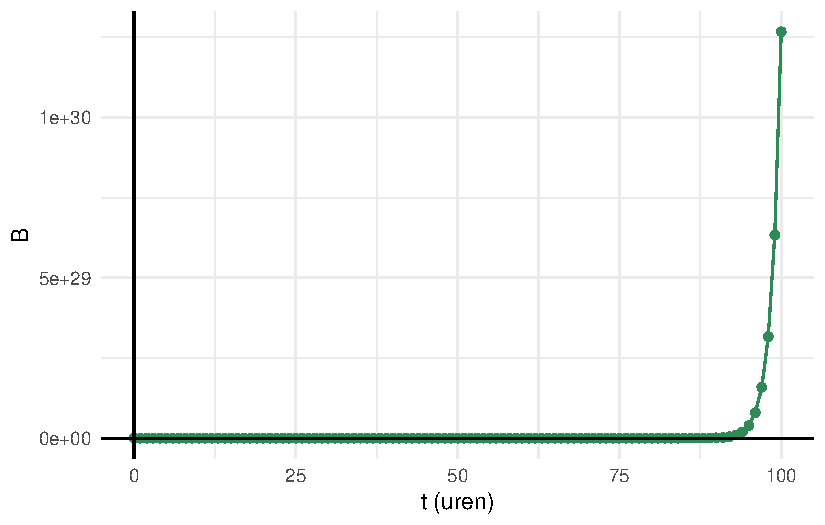
\includegraphics{Wiskunde/exponenten_files/figure-pdf/fig-logschaal-1.pdf}

}

}

\subcaption{\label{fig-logschaal-1}Op lineaire schaal.}
\end{minipage}%
%
\begin{minipage}[t]{0.50\linewidth}

{\centering 

\raisebox{-\height}{

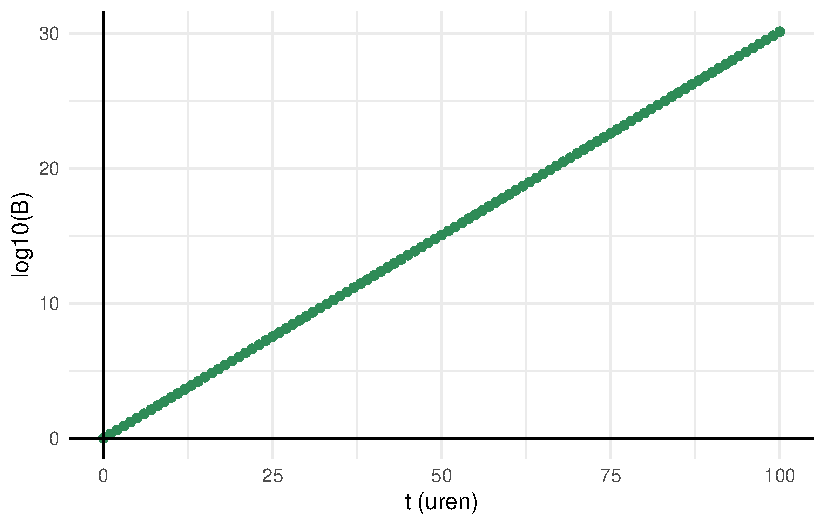
\includegraphics{Wiskunde/exponenten_files/figure-pdf/fig-logschaal-2.pdf}

}

}

\subcaption{\label{fig-logschaal-2}Op logaritmische schaal.}
\end{minipage}%

\caption{\label{fig-logschaal}Bacteriële groei over tijd.}

\end{figure}

\hypertarget{opdrachten-2}{%
\section{Opdrachten}\label{opdrachten-2}}

\begin{exercise}[]\protect\hypertarget{exr-exp-1}{}\label{exr-exp-1}

Schrijf in de vorm \(a^b\):

\textbf{a.} \(7^{345} \cdot 7^5 =\)

\textbf{b.} \(32^{20} \cdot 32^{18} =\)

\textbf{c.} \(2^5 \cdot 2^2 \cdot 2^3 =\)

\textbf{d.} \(3^{25} \cdot 3^{25} \cdot 3^{25} =\)

\end{exercise}

\begin{exercise}[]\protect\hypertarget{exr-exp-2}{}\label{exr-exp-2}

Los op:

\textbf{a.} \(\log{100} =\)

\textbf{b.} \(^2\log{64} =\)

\textbf{c.} \(^8\log{512} =\)

\textbf{d.} \(^5\log{125} =\)

\end{exercise}

\begin{exercise}[]\protect\hypertarget{exr-exp-3}{}\label{exr-exp-3}

~

\emph{Bacillus cereus} deelt elke 30 minuten. Je inoculeert een cultuur
met precies 100 bacteriën. Hoeveel bacteriën zijn er na 3 uur?

\end{exercise}

\begin{exercise}[]\protect\hypertarget{exr-exp-4}{}\label{exr-exp-4}

~

Een bacteriekolonie groeit onder ideale omstandigheden in het
labaratorium. Na 3 uur zijn er 10.000 bacteriën, en na 5 uur zijn het er
40.000. Met hoeveel bacteriën is de kolonie begonnen?\\
Tip: bepaal eerst wat de groeisnelheid van de kolonie is.

\end{exercise}

\begin{exercise}[]\protect\hypertarget{exr-exp-5}{}\label{exr-exp-5}

Los op voor x:

\textbf{a.} \(\log{2x} = 3\)

\textbf{b.} \(5e^x=11\)

\textbf{c.} \(^2\log{64^x}=36\)

\end{exercise}

\begin{exercise}[]\protect\hypertarget{exr-exp-6}{}\label{exr-exp-6}

~

Simplificeer de volgende uitdrukking, neem aan dat \(n\neq0\) en
\(p\neq0\):

\(\frac{(n^{-3})^4}{(n^{4}p^{-3})^{-3}}\).

\end{exercise}

\hypertarget{sec-limieten}{%
\chapter{Asymptoten \& Limieten}\label{sec-limieten}}

\hypertarget{introductie-3}{%
\section{Introductie}\label{introductie-3}}

Asymptoten zijn een wiskundig concept dat belangrijk kan zijn in
biologische modellen, vooral om te begrijpen hoe een functie zich
gedraagt wanneer de variabele heel groot of heel klein wordt. Dit is
vooral handig voor inzicht in biologische systemen op de langere
termijn.

Een asymptoot is een lijn, die door een functie wordt benaderd, maar
nooit precies bereikt. Bij het schetsen van een grafiek zijn asymptoten
vaak een handig hulpmiddel. Dit hoofdstuk beschrijft wat verticale en
horizontale asymptoten zijn en hoe je ze kunt vinden.

\hypertarget{horizontale-asymptoten}{%
\section{Horizontale asymptoten}\label{horizontale-asymptoten}}

Een horizontale asymptoot is een lijn met de vorm \(y=a\). De grafiek
benadert deze horizontale lijn voor hele grote of hele kleine waarden
van \(x\). Wiskundig heten deze ``hele grote'' en ``hele kleine''
waarden limieten.

De notatie hiervoor is als volgt:

\[\lim_{x \rightarrow +\infty}{f(x)} = a\]

Als de functie \(a\) benadert voor hele \textbf{grote} waarden van
\(x\), of: \[\lim_{x \rightarrow -\infty}{f(x)} = a\]

Als de functie \(a\) beandert voor hele \textbf{kleine} waarden van
\(x\). Zoals je uit deze notatie kunt aflezen kun je horizontale
asymptoten vinden door te kijken of de grafiek een waarde benadert voor
\(x \rightarrow \pm \infty\).

\hypertarget{voorbeeld}{%
\subsubsection*{Voorbeeld}\label{voorbeeld}}
\addcontentsline{toc}{subsubsection}{Voorbeeld}

Een voorbeeld van een functie met een horizontale asymptoot is:
\[f(x) = 5 + \frac{1}{x}\] Als we hele grote waarden voor \(x\) invullen
in deze functie, dan komt de uitkomst steeds dichter in de buurt van 5.
Dit geldt zowel voor grote positieve als negatieve waarden. Doordat
\(1\over x\) nooit gelijk aan 0 kan worden, zal \(f(x)\) nooit precies 5
worden. Daarom heeft deze functie een horizontale asymptoot \(y = 5\).

\begin{figure}

{\centering 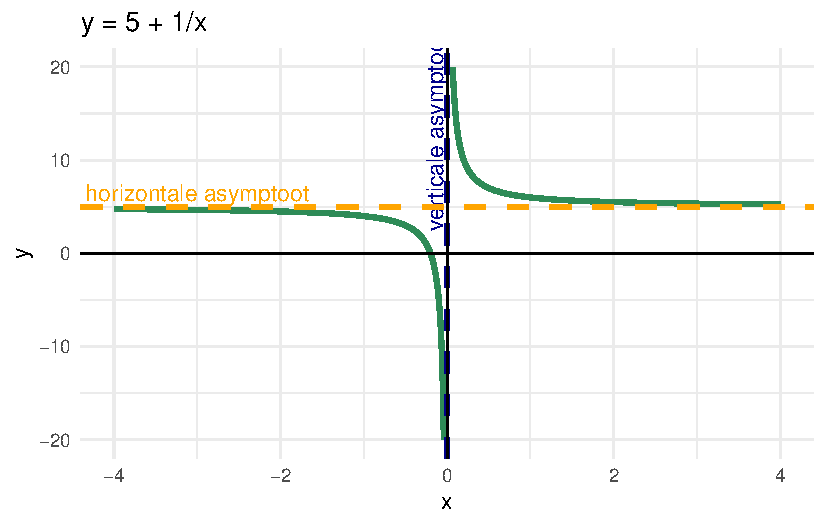
\includegraphics{Wiskunde/limieten_files/figure-pdf/fig-asymp-1.pdf}

}

\caption{\label{fig-asymp}De grafiek voor de functie y = 5 + 1/x. Deze
functie heeft zowel een horizontale als verticale asymptoot.}

\end{figure}

\hypertarget{verticale-asymptoten}{%
\section{Verticale asymptoten}\label{verticale-asymptoten}}

Een verticale asymptoot is een lijn met de vorm \(x=a\). Dit betekent
dat de waarde van \(f(x)\) voor \(x=a\) naar oneindig gaat. Dit kan
zowel plus als min oneindig zijn. In wiskundige notatie betekent dat:
\[\lim_{x \uparrow x_0}{f(x)} = \pm \infty\] als de asymptoot bereikt
wordt vanaf de ``linkerkant'' door x te verhogen tot \(x=a\). Of, als de
asymptoot vanaf de ``rechterkant'' bereikt wordt door x te verlagen tot
\(x=a\). \[\lim_{x \downarrow x_0}{f(x)} = \pm \infty\]

\hypertarget{voorbeeld-1}{%
\subsubsection*{Voorbeeld}\label{voorbeeld-1}}
\addcontentsline{toc}{subsubsection}{Voorbeeld}

De hierboven genoemde functie \(f(x) = 5 + \frac{1}{x}\) heeft niet
alleen een horizontale asymptoot, maar ook een verticale asymptoot. Dit
is vaak het geval bij functies waarbij de variabele in de noemer van een
breuk staat, omdat we niet kunnen delen door 0. Zoals je hebt geleerd is
delen hetzelfde als vermenigvuldigen met het omgekeerde. Delen door een
heel klein getal is dus hetzelfde als vermenigvuldigen met een heel
groot getal. Delen door 0 (oneindig klein), is dus hetzelfde als
vermendigvuldigen met oneindig. Omdat ``oneindig'' alleen als concept
bestaat, wordt er meestal gezegd dat de functie niet gedefiniëerd is
wanneer er door 0 gedeeld wordt.

Om de functie te kunnen schetsen, moeten we weten hoe het eruit ziet
rondom het punt \(x=0\). Als \(x\) net iets groter is dan 0, wordt
\(f(x)\) heel groot. Dit komt doordat delen door een heel klein positief
getal een hele grote positieve uitkomst geeft. Als we \(x=0\) benaderen
vanuit het negatieve domein, delen dan door een hele kleine negatieve
waarde, wat een hele grote negatieve uitkomst geeft.

Als we deze informatie combineren kunnen we \(f(x)\) schetsen:

\hypertarget{limieten-bepalen}{%
\section{Limieten bepalen}\label{limieten-bepalen}}

\hypertarget{limieten-voor-xto-infty}{%
\subsubsection*{\texorpdfstring{1. Limieten voor
\(x\to \infty\)}{1. Limieten voor x\textbackslash to \textbackslash infty}}\label{limieten-voor-xto-infty}}
\addcontentsline{toc}{subsubsection}{1. Limieten voor \(x\to \infty\)}

Wanneer \(x\) naar oneindig gaat, kun je niet simpelweg \(x= \infty\)
invullen, omdat oneindig geen getal is. Kijk in plaats daarvan naar het
gedrag van de functie voor grote waarden van \(x\).

\hypertarget{voorbeeld-2}{%
\subsubsection*{Voorbeeld}\label{voorbeeld-2}}
\addcontentsline{toc}{subsubsection}{Voorbeeld}

\[ \lim_{x \to \infty} 3 x^2 -5 = \infty\] Dit betekent dat de functie
steeds groter wordt naarmate \(x\) groter wordt. \textbar{} Voor
functies zoals \(f(x)=ax^3-bx^2\) moet je kijken naar de termen met de
hoogste macht van \(x\). In dit geval is dat \(ax^3\). Dit betekent dat
het positieve gedeelte van de functie (\(ax^3\)) sneller toeneemt dan
het negatieve gedeelte (\(-bx^2\)). De functie zal dus steeds groter
worden naarmate \(x\) groter wordt, dus:
\[ \lim_{x \to \infty} ax^3 - bx^2= \infty\]

\hypertarget{limieten-van-rationale-functies}{%
\subsubsection*{2. Limieten van rationale
functies}\label{limieten-van-rationale-functies}}
\addcontentsline{toc}{subsubsection}{2. Limieten van rationale functies}

Rationale functies zijn functies die een breuk bevatten, in de vorm
\(f(x)={p(x) \over g(x)}\). Bij het berekenen van limieten van deze
functies kun je de volgende regels toepassen:

\begin{longtable}[]{@{}
  >{\raggedright\arraybackslash}p{(\columnwidth - 2\tabcolsep) * \real{0.5444}}
  >{\raggedright\arraybackslash}p{(\columnwidth - 2\tabcolsep) * \real{0.4556}}@{}}
\toprule\noalign{}
\begin{minipage}[b]{\linewidth}\raggedright
Omschrijving
\end{minipage} & \begin{minipage}[b]{\linewidth}\raggedright
Wiskundige notatie
\end{minipage} \\
\midrule\noalign{}
\endhead
\bottomrule\noalign{}
\endlastfoot
Als je een constante deelt door \(x\), gaat de uitkomst naar 0 voor
grote waarden van \(x\) (\(x \rightarrow \infty\)) &
\(\lim_{x \to \infty } {C \over x} =0\) \\
Als je een constante deelt door \(x\), gaat de uitkomst naar \(\infty\)
wanneer \(x \rightarrow 0\) & \(\lim_{x \to 0 } {C \over x} =\infty\) \\
Als je \(x\) deelt door een constante, gaat de uitkomst naar \(\infty\)
voor grote waarden van \(x\) &
\(\lim_{x \to \infty } {x \over C} =\infty\) \\
Als je \(x\) deelt door een constante, gaat de uitkomst naar \(0\)
wanneer \(x \rightarrow 0\) & \(\lim_{x \to 0 } {x \over C} = 0\) \\
\end{longtable}

\hypertarget{snel-limieten-bepalen}{%
\subsubsection*{Snel limieten bepalen}\label{snel-limieten-bepalen}}
\addcontentsline{toc}{subsubsection}{Snel limieten bepalen}

\begin{enumerate}
\def\labelenumi{\arabic{enumi}.}
\tightlist
\item
  Vind de hoogste macht van \(x\) (of een andere variabele) in de
  functie.
\item
  De term met de hoogste macht zal de overhand spelen
\item
  Gaat deze term naar oneindig? Dan is de limiet oneindig. Gaat deze
  term naar 0? Dan is de limiet 0.
\end{enumerate}

\hypertarget{opdrachten-3}{%
\section{Opdrachten}\label{opdrachten-3}}

\begin{exercise}[]\protect\hypertarget{exr-asymp-1}{}\label{exr-asymp-1}

Bepaal de volgende limieten:

\textbf{a.} \(\lim_{x\to\infty}3x^2-2x+5\)

\textbf{b.} \(\lim_{ x \to 0+} {1 \over x}\) (let op: nadert 0 vanuit
het positieve domein)

\textbf{c.} \(\lim_{ x \to 0-} {1 \over x}\) (let op: nadert 0 vanuit
het negatieve domein)

\textbf{d.} \(\lim_{x \to \infty}{x \over x+2}\)

\textbf{e.} \(\lim_{x \to \infty}{1 \over a+x}\)

\textbf{f.} \(\lim_{x \to \infty}{(ax^2+b) \over cx^3}+d\)

\end{exercise}

\begin{exercise}[]\protect\hypertarget{exr-asymp-2}{}\label{exr-asymp-2}

Bepaal de asymptoten van de volgende functies:

\textbf{a.} \(f(x) = {x \over x-2} + 1\)

\textbf{b.} \(f(x) = {ax \over bx+c} - d\) waarbij \(d>a/b\)

\end{exercise}

\hypertarget{sec-afgeleiden}{%
\chapter{Afgeleiden}\label{sec-afgeleiden}}

\hypertarget{introductie-4}{%
\section{Introductie}\label{introductie-4}}

De afgeleide van een functie beschrijft hoe steil de functie is, oftewel
wat de richtingscoëfficiënt is. Een rechte lijn met de vorm \(y=ax+b\)
heeft voor elke \(x\)-waarde dezelfde richtingscoëfficiënt (\(a\)). We
kunnen daarom zeggen dat de afgeleide van \(y=ax+b\) gelijk is aan
\(y=a\). De afgeleide vertelt iets over hoe snel \(y\) verandert: hoe
hoger de richtingscoëfficiënt (\(a\)), hoe sneller \(y\) stijgt of
daalt.

De afgeleide van een lineaire vergelijking is dus een constante waarde
is die niet verandert voor verschillende \(x\)-waarden. Voor de meeste
vergelijkingen is dit echter niet het geval. Dit betekent dat de
afgeleide een functie is van \(x\). Met andere woorden: de grafiek heeft
niet voor elke \(x\)-waarde dezelfde richtingscoëfficiënt. Neem
bijvoorbeeld de vergelijking \(y = x^2 - 10\):

\begin{figure}

{\centering 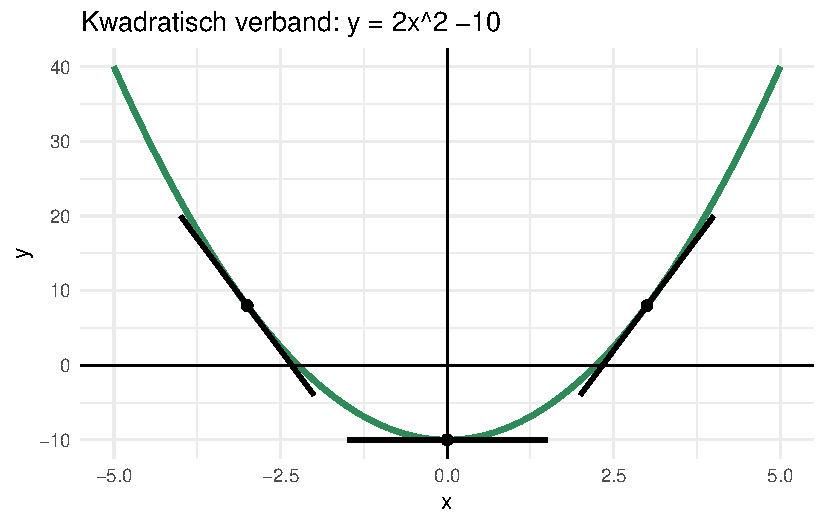
\includegraphics{Wiskunde/afgeleiden_files/figure-pdf/fig-afg-1.pdf}

}

\caption{\label{fig-afg}Grafiek van een kwadratisch verband (y = 2x\^{}2
+ 10). De grafiek is eerst dalend, dan vlak (bij x = 0), en daarna
stijgend.}

\end{figure}

De richtingscoëfficiënt varieert veel voor verschillende \(x\)-waarden:
de grafiek daalt eerst voor \(x<0\), loopt dan even horizontaal voor
\(x=0\), en stijgt steeds sneller voor \(x>0\). Met andere woorden: de
afgeleide is negatief voor lage waarde van \(x\), en positief voor
positieve waarden van \(x\). Als de afgeleide gelijk is aan \(0\), weten
we dat de functie een piek of een dal heeft.

De afgeleide van \(f(x)\) schrijven we als \(f'(x)\). Als \(f(x)\) de
positie van een fiets geeft, geeft \(f'(x)\) de snelheid van de fiets.
Eventueel kunnen we ook van deze snelheid \(f'(x)\) de afgeleide
bepalen, die wordt geschreven als \(f''(x)\). Deze staat dan voor de
versnelling van de fiets. Omdat biologische processen vaak omschreven
worden in termen van snelheden, is het belangrijk om begrip te hebben
van wat afgeleiden precies zijn. Echter, het is niet nodig om uit je
hoofd te weten hoe je afgeleiden precies bepaalt (zie hieronder een
overzicht, bij de toets krijg je de belangijkste regels op een
formuleblad).

\hypertarget{afgeleiden-van-veel-voorkomende-vergelijkingen}{%
\section{Afgeleiden van veel voorkomende
vergelijkingen}\label{afgeleiden-van-veel-voorkomende-vergelijkingen}}

\begin{longtable}[]{@{}
  >{\raggedright\arraybackslash}p{(\columnwidth - 6\tabcolsep) * \real{0.1751}}
  >{\raggedright\arraybackslash}p{(\columnwidth - 6\tabcolsep) * \real{0.3220}}
  >{\raggedright\arraybackslash}p{(\columnwidth - 6\tabcolsep) * \real{0.2712}}
  >{\raggedright\arraybackslash}p{(\columnwidth - 6\tabcolsep) * \real{0.2203}}@{}}
\toprule\noalign{}
\begin{minipage}[b]{\linewidth}\raggedright
Functie
\end{minipage} & \begin{minipage}[b]{\linewidth}\raggedright
Afgeleide
\end{minipage} & \begin{minipage}[b]{\linewidth}\raggedright
\(f(x)\)
\end{minipage} & \begin{minipage}[b]{\linewidth}\raggedright
\(f'(x)\)
\end{minipage} \\
\midrule\noalign{}
\endhead
\bottomrule\noalign{}
\endlastfoot
\(a\) & \(0\) & \(6\) & \(0\) \\
\(ax\) & \(a\) & \(7x\) & \(7\) \\
\(ax^b\) & \(b \cdot a x^{b-1}\) & \(8x^3\) & \(24x^2\) \\
\(c \cdot f(x)\) & \(c \cdot f'(x)\) & \(2x^{13}\) &
\(2 \cdot 13x^{12} = 26x^{12}\) \\
\(f(x) + g(x)\) & \(f'(x) + g'(x)\) & \(x^4 + 4x\) & \(4x^3 + 4\) \\
\(e^x\) & \(e^x\) & \(e^x\) & \(e^x\) \\
\(a e^{bx}\) & \(b \cdot a e^{bx}\) &
\(\frac{1}{2} \cdot \pi \sqrt{2} \cdot e^{2x}\) &
\(\pi \sqrt{2} \cdot e^{2x}\) \\
\(e^{f(x)}\) & \(f'(x) \cdot e^{f(x)}\) & \(e^{2x^2 - x}\) &
\((4x - 1) \cdot e^{2x^2 - x}\) \\
\(a^{f(x)}\) & \(\ln(a) \cdot f'(x) \cdot a^{f(x)}\) & \(5^{4x - 1}\) &
\(\ln(5) \cdot 4 \cdot 5^{4x - 1}\) \\
\(\ln(x)\) & \(\frac{1}{x}\) & \(\ln(x)\) & \(\frac{1}{x}\) \\
\(\ln(a x) = \ln(a) + \ln(x)\) & \(\frac{1}{x}\) &
\(\ln(4x) = \ln(4) + \ln(x)\) & \(\frac{1}{x}\) \\
\(f(x) \cdot g(x)\) & \(f'(x) \cdot g(x) + f(x) \cdot g'(x)\) &
\((x^2 - 4)(x^3 + 2x + 3)\) & \(5x^4 - 6x^2 + 6x - 8\) \\
\(\frac{f(x)}{g(x)}\) &
\(\frac{g(x) \cdot f'(x) - f(x) \cdot g'(x)}{(g(x))^2}\) &
\(\frac{4x + 1}{x^2 + 1}\) & \(\frac{-4x^2 - 2x + 4}{(x^2 + 1)^2}\) \\
\end{longtable}

\hypertarget{opdrachten-4}{%
\section{Opdrachten}\label{opdrachten-4}}

\begin{exercise}[]\protect\hypertarget{exr-afg-1}{}\label{exr-afg-1}

Bereken de afgeleide van de volgende functies:

\textbf{a.} \(f(x)=x^2+15x\)

\textbf{b.} \(f(x)=12x^5-6\)

\textbf{c.} \(f(x)=\frac{7}{x^4}\)

\textbf{d.} \(f(x)=ax^3-bx^5\)

\end{exercise}

\begin{exercise}[]\protect\hypertarget{exr-afg-2}{}\label{exr-afg-2}

Bekijk de hierboven gegeven tabel met afgeleiden van veel voorkomende
vergelijkingen. Leg in je eigen woorden waarom het nuttig kan zijn om
exponentiële groei op te schrijven met grondtal \(e\) (het getal van
Euler).

\end{exercise}

\hypertarget{sec-schetsen}{%
\chapter{Functies schetsen}\label{sec-schetsen}}

\hypertarget{introductie-5}{%
\section{Introductie}\label{introductie-5}}

Functies laten zien hoe variabelen met elkaar samenhangen. Bijvoorbeeld,
\(y=f(x)\) kan beschrijven hoe zwaar iemand gemiddeld is (\(y\) is het
gewicht) op basis van hun lengte (\(x\) is de lengte). Of het kan laten
zien hoeveel bacteriën er zijn (\(y\)) na verloop van tijd (\(x\)).
Functies zijn dus een belangrijk middel om gegevens te beschrijven en
samen te vatten.

Om te begrijpen wat een functie \(f(x)\) laat zien, is het nuttig om de
grafiek ervan te kunnen tekenen. Hiervoor moeten we een aantal
belangrijke punten van de functie bepalen: eigenschappen zoals
snijpunten met de x- en y-as, asymptoten, en waar eventuele toppen of
dalen liggen. Dit vereist technieken zoals het oplossen van
vergelijkingen, het vinden van limieten en het berekenen van afgeleiden,
zoals eerder besproken.

\hypertarget{veelvoorkomende-functies}{%
\section{Veelvoorkomende functies}\label{veelvoorkomende-functies}}

Functies worden vaak weergegeven door hun grafiek. Hierbij zetten we de
waarden van \(x\) op de x-as en de waarde van de functie \(f(x)\) op de
y-as. Hieronder staan enkele veelvoorkomende grafieken.

\hypertarget{grafieken-van-een-constante-functie}{%
\subsection*{Grafieken van een constante
functie}\label{grafieken-van-een-constante-functie}}
\addcontentsline{toc}{subsection}{Grafieken van een constante functie}

De grafiek van een functie van de vorm \(y=p\) is een \emph{horizontale}
lijn die de y-as snijdt op de waarde \(p\). In plaats daarvan kunnen we
ook vinden dat \(x=q\), wat een \emph{verticale} lijn is die de x-as
snijdt op de waarde \(q\). (NOTE FOR MADELON: ALLEBEI IN 1 PLAATJE?)

\begin{figure}

{\centering 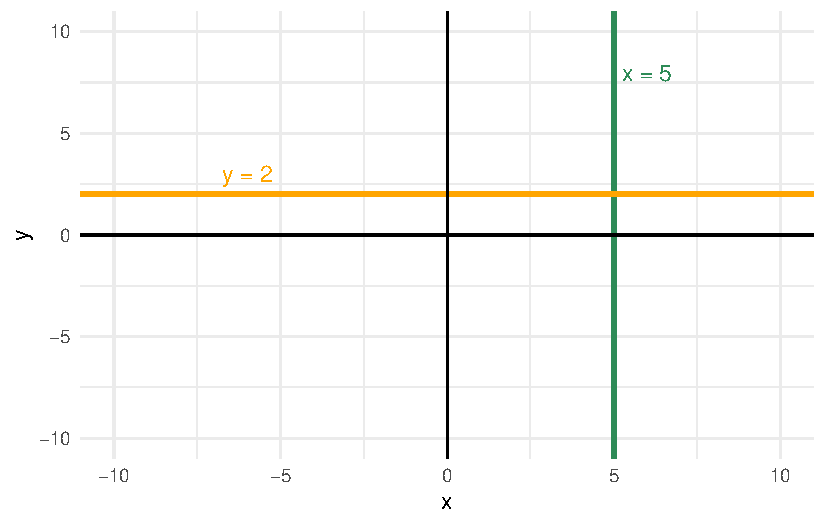
\includegraphics{Wiskunde/schetsen_files/figure-pdf/fig-draw-line-1.pdf}

}

\caption{\label{fig-draw-line}De grafiek voor de functie y = 2 is een
rechte horizontale lijn. De grafiek voor de functie x = 5 is een rechte
verticale lijn.}

\end{figure}

\hypertarget{grafieken-van-lineaire-functies}{%
\subsection*{Grafieken van lineaire
functies}\label{grafieken-van-lineaire-functies}}
\addcontentsline{toc}{subsection}{Grafieken van lineaire functies}

De grafiek van een lineaire functie \(y=ax+b\) is een rechte lijn met
helling \(a\) en snijpunt \(b\) op de y-as. Dat laatste kun je zien door
\(x=0\) in te vullen: op dit moment snijdt je de y-as! Als \(a>0\),
loopt de lijn stijgend; bij \(a<0\) daalt de lijn. Hoe groter \(|a|\),
hoe steiler de lijn.

\begin{figure}

{\centering 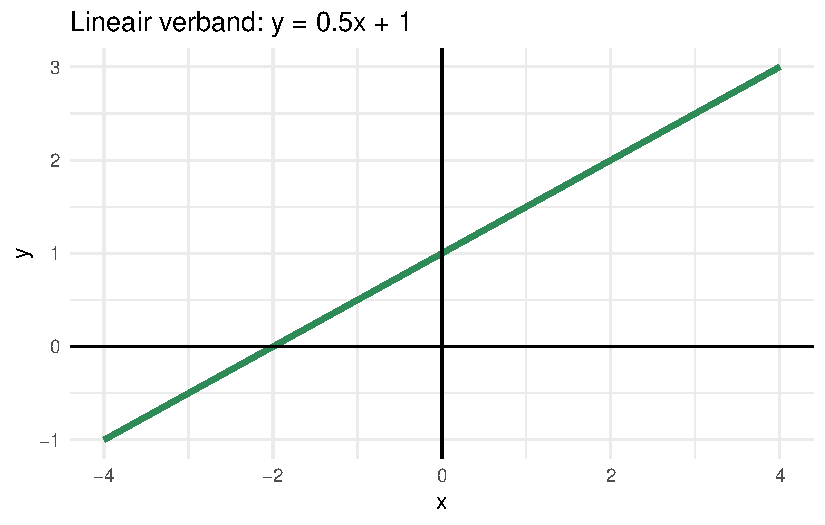
\includegraphics{Wiskunde/schetsen_files/figure-pdf/fig-algebra-lineair-1.pdf}

}

\caption{\label{fig-algebra-lineair}Voorbeeld lineair verband.}

\end{figure}

\hypertarget{grafieken-van-kwadratische-functies}{%
\subsection*{Grafieken van kwadratische
functies}\label{grafieken-van-kwadratische-functies}}
\addcontentsline{toc}{subsection}{Grafieken van kwadratische functies}

De grafiek van de kwadratische vergelijking \(y=ax^2+bx+c\) is een
parabool. Bij \(a>0\) opent de parabool naar boven (dalparabool), bij
\(a<0\) naar beneden (bergparabool). De waarden van \(a\), \(b\) en
\(c\) bepalen hoe de parabool ligt. Met de abc-formule kun je vinden
wanneer de functie \(0\) is. Dit zijn de snijpunten met de x-as. Door
\(x=0\) in te vullen vindt je het snijpunt met de y-as (hier: \(c\)).
Door de afgeleide te vinden en deze gelijk te stellen aan \(0\) vind je
waar de piek of het dal ligt.

\begin{figure}

{\centering 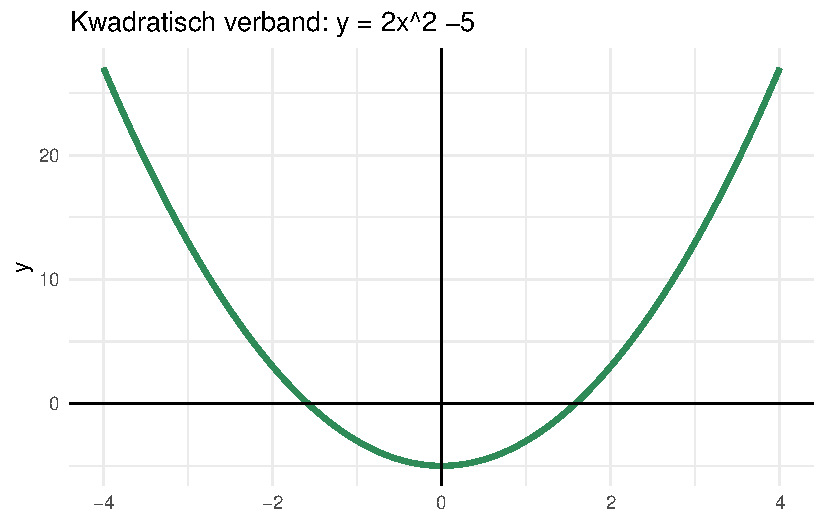
\includegraphics{Wiskunde/schetsen_files/figure-pdf/fig-algebra-kwadratisch-1.pdf}

}

\caption{\label{fig-algebra-kwadratisch}Voorbeeld kwadratisch verband.}

\end{figure}

\hypertarget{grafieken-van-machtsfuncties}{%
\subsection*{Grafieken van
machtsfuncties}\label{grafieken-van-machtsfuncties}}
\addcontentsline{toc}{subsection}{Grafieken van machtsfuncties}

Grafieken van functies zoals \(x^a\) veranderen van hellingshoek naar
mate \(x\) groter of kleiner wordt. Als {\(a>1\)}, dan neemt de
helingshoek toe, en . Als {\(0<a<1\)} (als \(a\) tussen 0 en 1 ligt),
neemt de helingshoek af. Als {\(a=1\)}, dan blijft de hellingshoek
gelijk, want dan is de functie precies gelijk aan \(y=x\).

\begin{figure}

{\centering 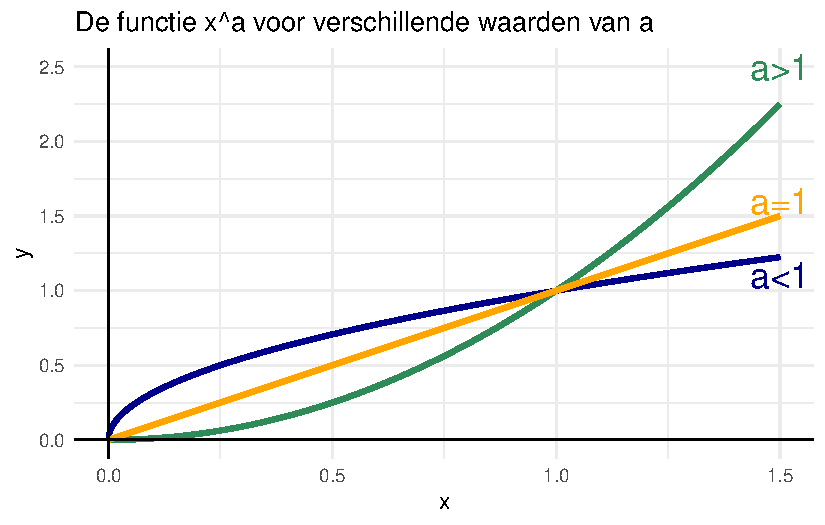
\includegraphics{Wiskunde/schetsen_files/figure-pdf/fig-draw-machtsfuncties-1.pdf}

}

\caption{\label{fig-draw-machtsfuncties}De grafiek van de functie x\^{}a
is een rechte lijn voor a = 1, convex voor a \textgreater{} 1 en concaaf
voor a \textless{} 1.}

\end{figure}

\hypertarget{stappenplan-functies-schetsen}{%
\section{Stappenplan functies
schetsen}\label{stappenplan-functies-schetsen}}

\begin{enumerate}
\def\labelenumi{\arabic{enumi}.}
\tightlist
\item
  Vind de \textbf{snijpunten met de} \(x\)-as door \(y = f(x) = 0\) op
  te lossen.
\item
  Vind de \textbf{snijpunten met de} \(y\)-as door \(x=0\) in te vullen
  in \(y = f(x)\).
\end{enumerate}

\begin{tcolorbox}[enhanced jigsaw, coltitle=black, breakable, bottomtitle=1mm, opacityback=0, colback=white, rightrule=.15mm, title=\textcolor{quarto-callout-tip-color}{\faLightbulb}\hspace{0.5em}{Tip}, bottomrule=.15mm, toprule=.15mm, left=2mm, colframe=quarto-callout-tip-color-frame, toptitle=1mm, opacitybacktitle=0.6, titlerule=0mm, colbacktitle=quarto-callout-tip-color!10!white, leftrule=.75mm, arc=.35mm]

Niet elke functie heeft een snijpunt met de \(x\)- en/of \(y\)-as.

\end{tcolorbox}

\begin{enumerate}
\def\labelenumi{\arabic{enumi}.}
\setcounter{enumi}{2}
\tightlist
\item
  Vind \textbf{horizontale asymptoten} door de limieten
  \(y = \lim x \to \pm \infty\) te berekenen.
\item
  Voor rationale functies, met de vorm \(f(x) = {p(x) \over q(x)}\),
  vind \textbf{verticale asymptoten} door te bepalen of er waarden voor
  \(x\) zijn waarvoor \(q(x)=0\) (en dus \(f(x) \to \pm \infty\)). Deze
  \(x\)-waarden zijn verticale asymptoten van de functie.
\item
  Vind \textbf{minima en maxima} door te bepalen voor welke
  \(x\)-waarden geldt dat \(f'(x)=0\). Bepaal vervolgens de \(y\)-waarde
  van deze minima en maxima door de gevonden \(x\)-waarden in te vullen
  in \(f(x)\).
\end{enumerate}

\begin{tcolorbox}[enhanced jigsaw, coltitle=black, breakable, bottomtitle=1mm, opacityback=0, colback=white, rightrule=.15mm, title=\textcolor{quarto-callout-tip-color}{\faLightbulb}\hspace{0.5em}{Tip}, bottomrule=.15mm, toprule=.15mm, left=2mm, colframe=quarto-callout-tip-color-frame, toptitle=1mm, opacitybacktitle=0.6, titlerule=0mm, colbacktitle=quarto-callout-tip-color!10!white, leftrule=.75mm, arc=.35mm]

Als je twijfelt of een functie stijgt of daalt voor bepaalde
\(x\)-waarden kun je gebruikmaken van de afgeleide voor die
\(x\)-waarden. Als \(f'(x) > 0\) dan stijgt de functie rond die
\(x\)-waarde. Als \(f'(x) < 0\) dan daalt de functie rond die
\(x\)-waarde.

\end{tcolorbox}

\begin{figure}

{\centering 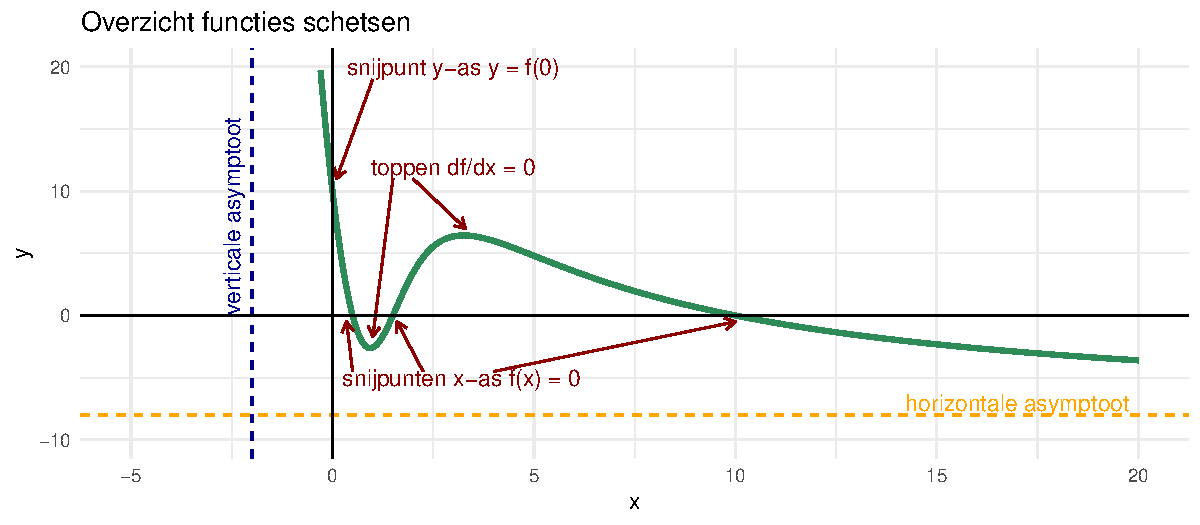
\includegraphics{Wiskunde/schetsen_files/figure-pdf/fig-draw-overzicht-1.pdf}

}

\caption{\label{fig-draw-overzicht}Overzicht van alle hulpmiddelen die
nuttig zijn bij het schetsen van een functie.}

\end{figure}

\hypertarget{opdrachten-5}{%
\section{Opdrachten}\label{opdrachten-5}}

\begin{exercise}[]\protect\hypertarget{exr-draw-1}{}\label{exr-draw-1}

Gebruik het bovenstaande stappenplan om de volgende functies te
schetsen:

\textbf{a.} \(y=3-6x\)

\textbf{b.} \(y=px+q\), neem aan dat \(p>0\) en \(q>0\)

\textbf{c.} \(y=x-3x^2\)

\textbf{d.} \(y=(a-x) \cdot (b-x) \cdot (c-x)\), neem aan dat
\(a,b,c>0\) en \(a<b<c\), namelijk \(b=2 \cdot a\) en \(c=3 \cdot a\)

\textbf{e.} \(y=x^3-5x^2\)

\textbf{f.} \(y=\frac{4x}{x+2}+4\)

\end{exercise}

\begin{exercise}[]\protect\hypertarget{exr-draw-2}{}\label{exr-draw-2}

We zijn vaak gewend dat x op de horizontale as staat, en y op de
verticale as. Soms staat het echter helemaal niet vast wat we precies op
welke as moeten schetsen (of heten de variabelen helemaal geen x- en
y!).

Stel we vinden een verband tussen het aantal konijnen (\(K\)) en het
aantal vossen (\(V\)) omschreven door de functie \(K = a - b \cdot V\).

\textbf{a.} Hoeveel konijnen zijn er als er geen vossen zijn? Wat is
effect van vossen op de hoeveelheid konijnen?

\textbf{b.} Teken een assenstelsel met \(K\) op de x-as, en \(V\) op de
y-as. Probeer de functie \(K = a - b \cdot V\) te schetsen.

\textbf{c.} Herschrijf \(K = a - b \cdot V\) zodat het aantal vossen
wordt uitgedrukt als een functie van het aantal konijnen. Schets nu ook
deze functie in je assenstelsel. Wat valt je op?

\textbf{d.} Als we meteen het aantal konijnen op de y-as hadden gezet,
hadden we dan de functie hoeven herschrijven?

\end{exercise}

\part{Biologische modellen}

\hypertarget{sec-tbintro}{%
\chapter{Introductie}\label{sec-tbintro}}

\hypertarget{leerdoelen}{%
\section{Leerdoelen}\label{leerdoelen}}

Aan het eind van dit introducerende hoofdstuk, word je geacht
hetvolgende te kunnen:

\begin{itemize}
\tightlist
\item
  Uitleggen waarom modellen een belangrijk stuk gereedschap zijn binnen
  de biologie
\item
  De drie basisingrediënten van elk model benoemen
\item
  Onderscheid maken tussen onderwerp (\emph{wat} gemodelleerd wordt) en
  model-formalismes (\emph{hoe} er gemodelleerd wordt)
\item
  Voorbeelden van verschillende model-formalismes geven, en alvast
  enkele aannames die erbij komen kijken benoemen (nog niet in detail:
  gedurende de cursus leer je meer over de details)
\item
  Uitleggen wanneer je een model ``goed'' kan noemen
\end{itemize}

\hypertarget{onze-intuuxeftie-is-niet-genoeg}{%
\section{Onze intuïtie is niet
genoeg}\label{onze-intuuxeftie-is-niet-genoeg}}

Waarom zijn er het ene jaar zoveel meer konijnen dan het andere jaar?
Hoe worden de patronen op de huid van een zebravis aangelegd? Komt het
beschieten van dieren in de Oostvaarderseplassen hun welzijn ten goede?
Waarom werken individuen van dezelfde soort samen, en vergt dit gedrag
een complexe sociale structuur? Wat is er aan de hand tijdens een
hartritmestoornis, en op welke manieren kunnen we het hart herstellen?
Dit zijn allemaal belangrijke biologische vraagstukken, maar zoals
jullie allemaal weten zijn biologische systemen vaak erg ingewikkeld. In
het vakgebied Theoretische Biologie worden daarom modellen en simulaties
gebruikt, om zodoende nieuwe inzicht in te vergaren en betere
voorspellingen te doen. Omdat modellen een steeds belangrijker onderdeel
zijn van de biologie, is het voor elke bioloog belangrijk om de nodige
basiskennis te hebben.

\begin{figure}

{\centering 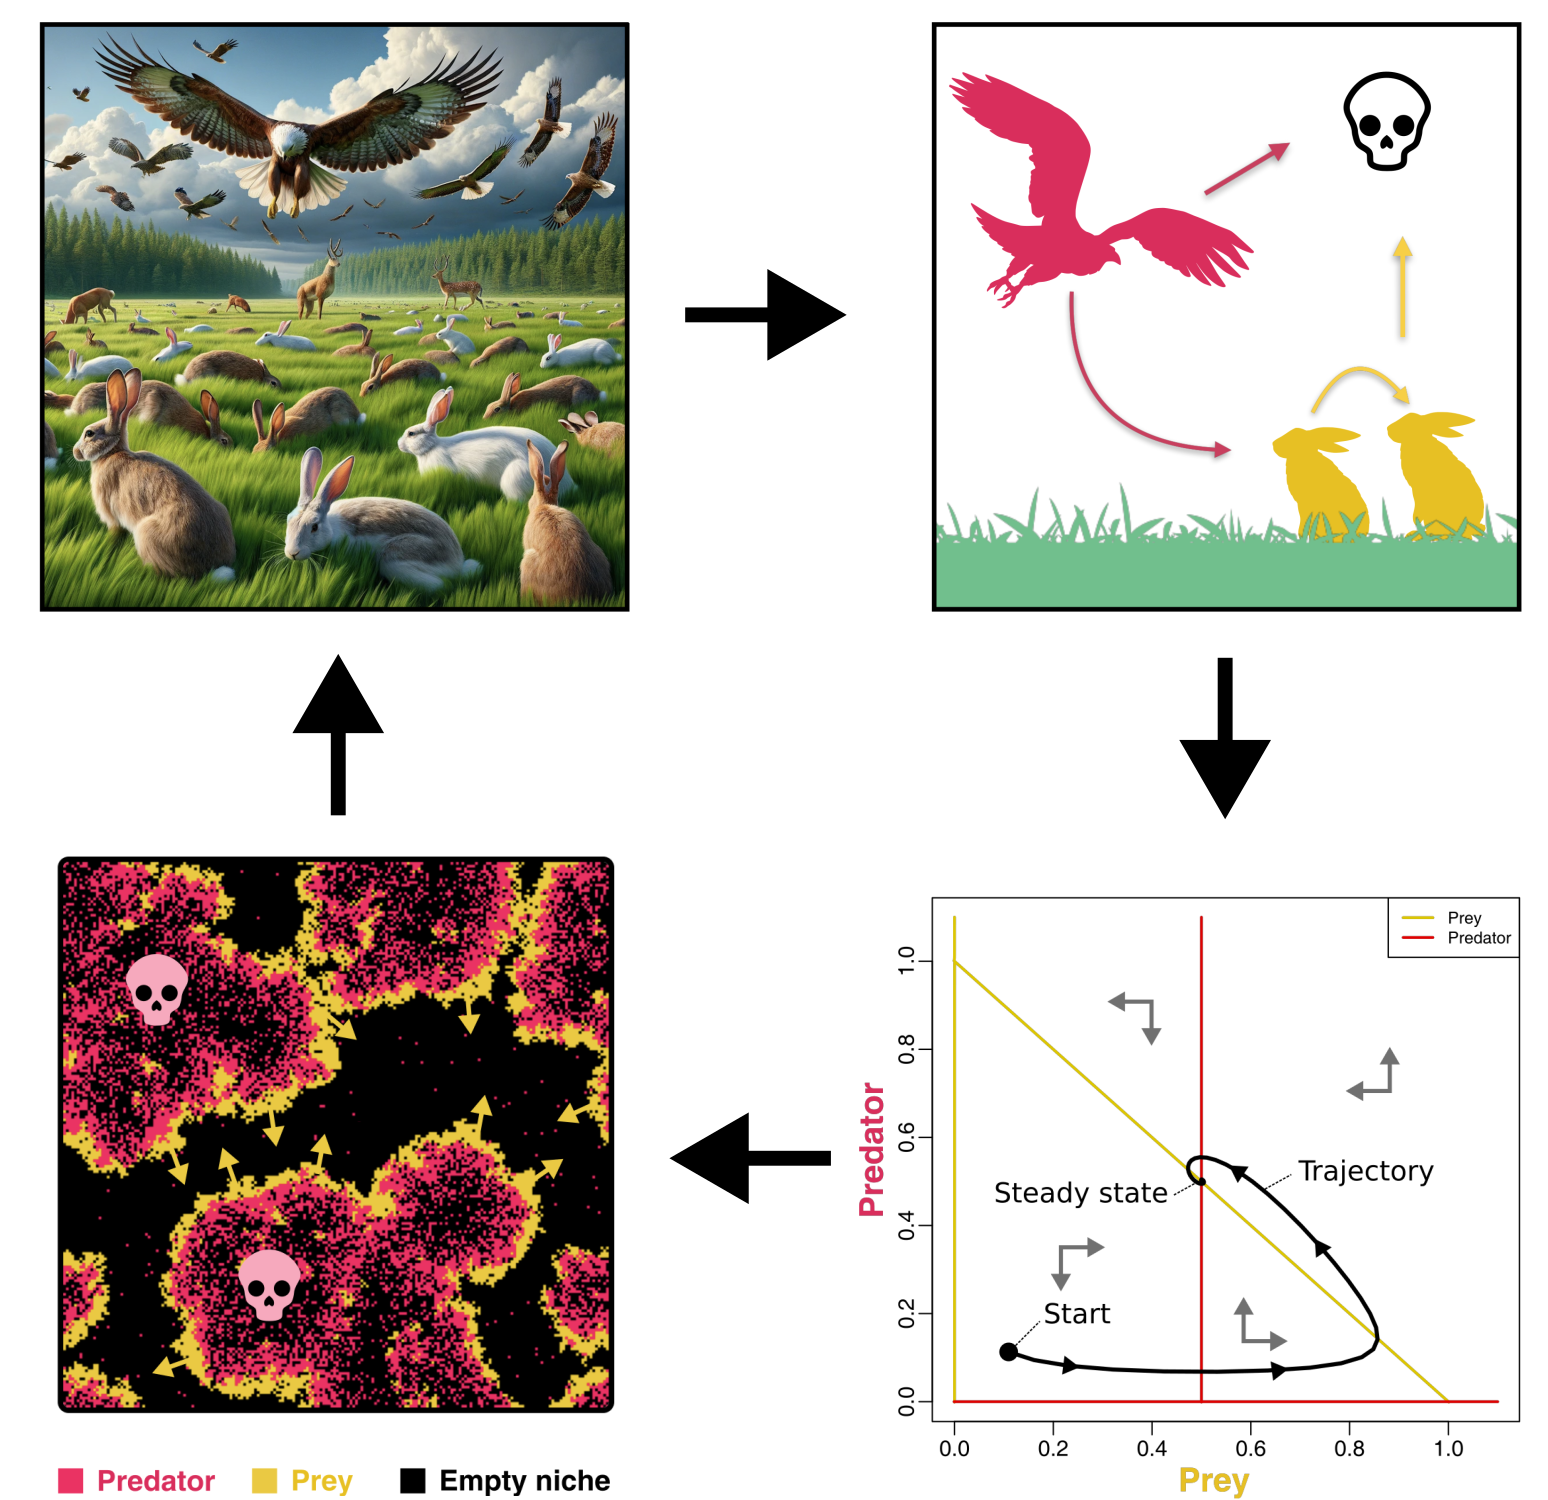
\includegraphics[width=0.8\textwidth,height=\textheight]{Modellering/../Modellering/figuren/cover.png}

}

\end{figure}

Om echt goed te begrijpen wat een model is, gaan we helemaal bij de
basis beginnen en de meest simpele modellen bespreken. Je zal zien dat
zelfs \emph{simpele} modellen zich vaak onvoorspelbaar en tegenintuïtief
kunnen gedragen. Onze intuïtie is dus niet te vertrouwen! Het is dus
belangrijk om te leren hoe je modellen moet lezen (wiskunde en simpele
R-scripts), en welke conclusies je er wel/niet uit kan trekken. Om dit
te leren, bespreken we modellen uit verschillende vakgebieden binnen de
biologie (microbiologie, ecologie, gedrag, evolutie). Wat je favoriete
onderwerp ook is: je komt als bioloog -- ook na deze cursus -- zeer
zeker nog meer met modellen in aanraking!

Dit cursusonderdeel is verdeeld over drie kernmodules (in ongeveer drie
weken):

\begin{enumerate}
\def\labelenumi{\arabic{enumi}.}
\tightlist
\item
  Module 1: Populatiegroei
\item
  Module 2: Ecologie, competitie, en evolutie
\item
  Module 3: Gedrag, diffusie, en emergente patronen
\end{enumerate}

Maar voordat we aan deze modules beginnen, wil ik jullie eerst graag
uitleggen introduceren wat modellen nou eigenlijk \textbf{zijn}.

\begin{figure}

{\centering 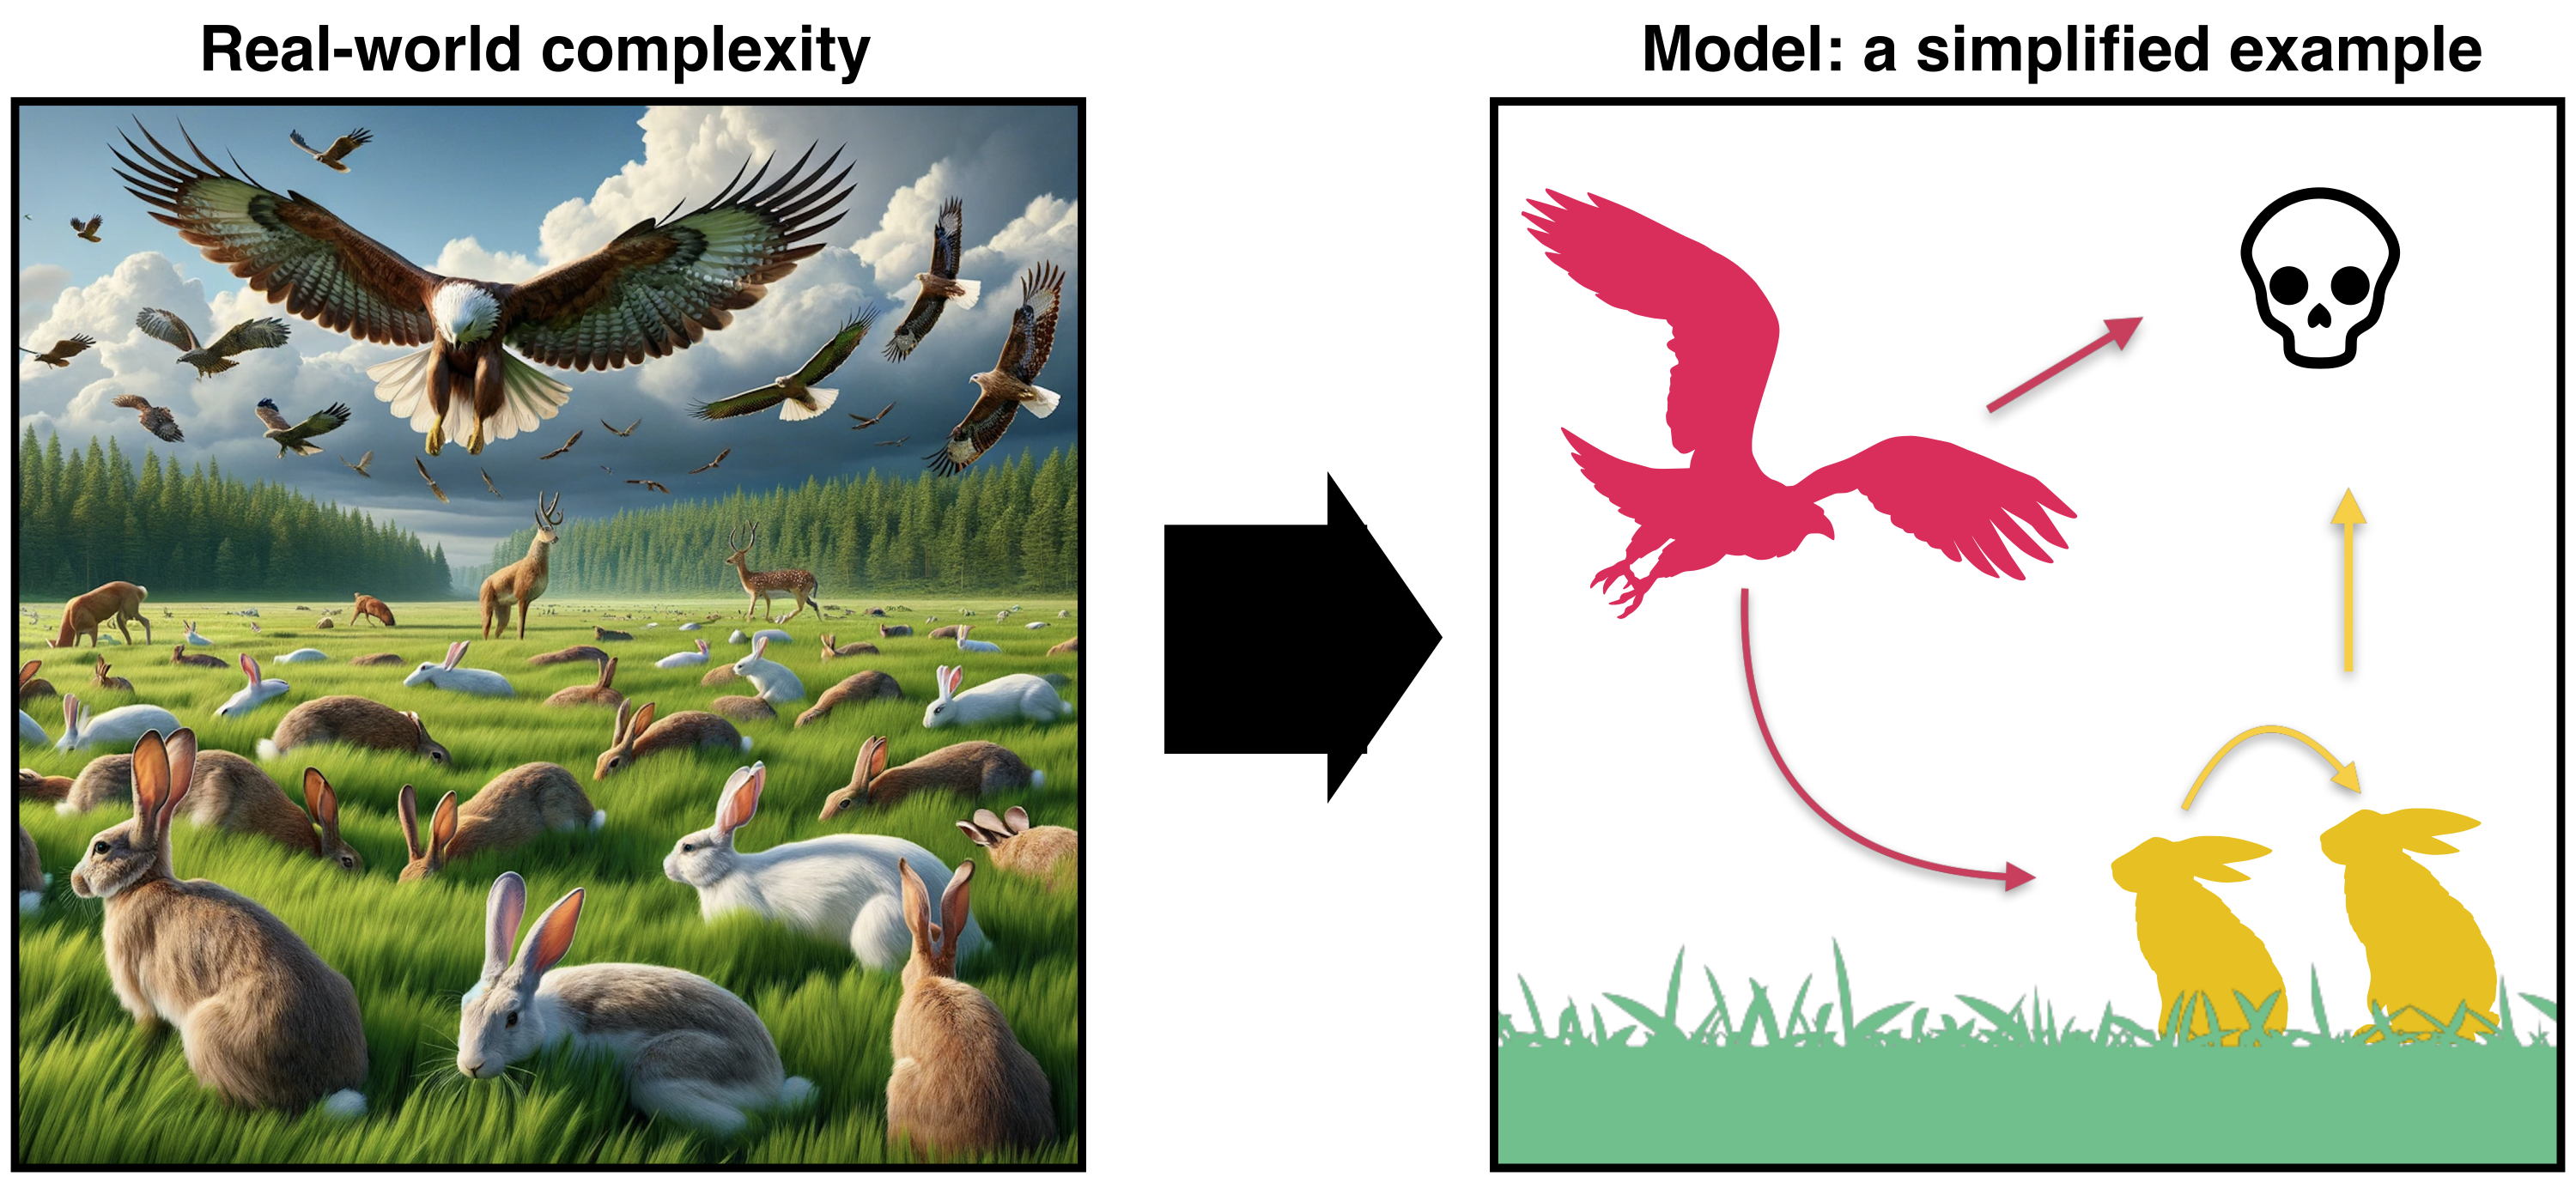
\includegraphics{Modellering/../Modellering/figuren/modelling.png}

}

\caption{\label{fig-veluwe}Modellen zijn versimpelde voorbeelden van
complexe situaties. Door deze versimpeling te bestuderen kunnen we
dingen leren over biologie}

\end{figure}

Stel je voor dat je op de Veluwe aan het wandelen bent, en het scenario
tegenkomt aan de linker zijde van Figuur~\ref{fig-veluwe}: overal lopen
verschillend gekleurde konijnen, roofvogels vliegen rond en grijpen hun
kans, en in de achtergrond zie je herten, naaldbossen, en duistere
wolken. Hoewel dit scenario natuurlijk een enorme karikatuur is, worden
we in de biologie wel vaak geconfronteerd met dit probleem: biologische
systemen bestaan uit veel onderdelen die allemaal tegelijk elkaar
beïnvloeden. Om dit een beetje behapbaar te maken, kunnen we ervoor
kiezen om het systeem versimpelen. Zo zie je aan de rechter zijde van
\textbf{Figuur~\ref{fig-veluwe}} dat we de achtergrond (herten, bos,
wolken) even vergeten, en ons richten op slechts een paar onderdelen.
Wellicht zijn we vooral geïnteresseerd in de interacties tussen de
roofvogels en de konijnen. De roofvogels jagen op konijnen, terwijl de
konijnen doen waar konijnen goed in zijn: vermenigvuldigen.

In de biologie zijn we veelal geïnteresseerd in de \textbf{dynamiek} van
systemen. Dat betekent: hoe verandert het systeem over de tijd? In het
voorbeeld van de roofvogels en konijnen, kunnen we ons bijvoorbeeld
afvragen welk van de twee soorten zal toenemen, en welke zal afnemen. Je
kunt je natuurlijk wel voorstellen dat als er heel veel konijnen zijn,
dat de roofvogels dan een enorme kans hebben konijnen te vangen, en dus
in populatiegrootte zullen toenemen. Echter zal dit het aantal konijnen
verlagen\ldots{} wat gebeurt er daarna? Sterven alle konijnen uit?
Kunnen ze samen voortbestaan? Het antwoord hangt af van bepaalde keuzes
die we moeten maken. Modelleren we alleen roofvogels en konijnen, of ook
het gras dat door konijnen gegeten wordt? Hoe lang leven de roofvogels
eigenlijk? En gaan de konijnen ook van ouderdom dood, of worden deze
vooral door roofvogels opgegeten? Bij al deze verschillende keuzes komt
belangrijke terminologie kijken die de basis vormen van elk model:
\textbf{variabelen}, \textbf{parameters}, en \textbf{aannames}
(\emph{assumptions}).

\begin{tcolorbox}[enhanced jigsaw, coltitle=black, breakable, bottomtitle=1mm, opacityback=0, colback=white, rightrule=.15mm, title=\textcolor{quarto-callout-note-color}{\faInfo}\hspace{0.5em}{Nederlands (\emph{Dutch})}, bottomrule=.15mm, toprule=.15mm, left=2mm, colframe=quarto-callout-note-color-frame, toptitle=1mm, opacitybacktitle=0.6, titlerule=0mm, colbacktitle=quarto-callout-note-color!10!white, leftrule=.75mm, arc=.35mm]

Net zoals bij elk vakgebied, komen er bij modellen nogal wat nieuwe
termen kijken. Dit jargon is niet altijd goed in het Nederlands te
vertalen, en daarnaast zijn de Engelse termen vaak heel handig om te
kennen. Om jullie daarmee te helpen, zullen we toch vaak het Engelse
jargon gebruiken. Aan het einde van ieder hoofdstuk staat een tabel met
de vertaling van deze termen.

\end{tcolorbox}

\hypertarget{de-basisingrediuxebnten-van-elk-model}{%
\section{De basisingrediënten van elk
model}\label{de-basisingrediuxebnten-van-elk-model}}

Modellen in de biologie kunnen heel simpel zijn, maar soms ook vrij
complex zijn. Hoe ingewikkeld of simpel een model ook is, de
basisingrediënten veranderen eigenlijk nauwelijks. Elk model draait om:

\begin{itemize}
\item
  \textbf{Variabelen} (\emph{variables}): hetgeen wat er verandert
  (bijvoorbeeld over de tijd). In het voorbeeld hierboven zouden dat
  bijvoorbeeld de populatiegroottes van de konijnen en/of roofvogels
  kunnen zijn.
\item
  \textbf{Parameters} (\emph{parameters}): constante waarden die bepalen
  \emph{hoe} variabelen veranderen, bijvoorbeeld de groeisnelheid van de
  konijnen. In plaats van deze getallen vast te zetten (bijv.
  groeisnelheid = 2) gebruiken we meestal zogenoemde ``vrije
  parameters'\,' (bijv. groeisnelheid = \(r\)). Let op: in biologische
  modellen nemen we over het algemeen aan dat dergelijke parameters
  positief zijn.
\item
  \textbf{Aannames} (\emph{assumptions}): keuzes die we maken om het
  model eenvoudig te houden. In het voorbeeld hierboven negeren we
  bijvoorbeeld de herten, het bos op de achtergrond, en we zouden ook
  kunnen kiezen om alle konijnen in het model identiek te laten zijn,
  ook al zien we variaties in hun kleur.
\end{itemize}

Aan het eind van dit cursusonderdeel zul je begrijpen dat de
bovengenoemde begrippen gebruikt kunnen worden om allerlei biologische
scenario's simpeler te omschrijven. Door deze versimpelingen te
bestuderen, proberen we wat te leren over biologie. Maar afhankelijk van
de biologische situatie kan het zijn dat aannames meer of minder gepast
zijn.

Aan het \emph{eind} van elk hoofdstuk staan lange verdiepende vragen,
die we in het werkcollege behandelen. Tussen het lezen door staan echter
ook wat kortere vragen, zodat je kan inschatten of je de stof goed tot
je hebt genomen. Dus hierbij:

\begin{exercise}[Bloedsuikerspiegel tijdens het
sporten]\protect\hypertarget{exr-variabelen-en-parameters}{}\label{exr-variabelen-en-parameters}

Tijdens het sporten daalt de bloedsuikerspiegel \(a\) met een vaste
snelheid \(b\), waarbij een eiwit \(c\) tot expressie komt met vaste
snelheid \(d\).

\textbf{a.} Welke van de symbolen (\(a\), \(b\), \(c\), en \(d\)) zou je
als variabelen kunnen beschouwen, en waarom?

\textbf{b.} Welke van de symbolen zou je eerder als parameters
beschouwen, en waarom?

\end{exercise}

Nu we een idee hebben wat paramteres, variabelen, en aannames precies
zijn, gaan we een paar voorbeeld-scenarios bespreken. Let op: deze
voorbeelden hoef je nu nog niet 100\% te begrijpen, en dienen op dit
punt vooral ter illustratie.

\hypertarget{een-verschillend-model-voor-elk-scenario}{%
\section{Een verschillend model voor elk
scenario}\label{een-verschillend-model-voor-elk-scenario}}

Niet alle modellen zien er hetzelfde uit. Veel modellen gebruiken
simpele wiskundige formules om verandering over de tijd te omschrijven.
Zo zouden we de jaarlijkse populatiegrootte van een bedreigde
vlindersoort (zie Figuur~\ref{fig-modeltypes} A) kunnen omschrijven in
een differentievergelijking (\emph{Difference Equation,} ook wel map
genoemd). Deze vergelijking omschrijft simpelweg een relatie tussen de
huidige waarde van de variabele \(V(t)\) (hoeveelheid vlinders in dit
jaar) en de toekomstige waarde van de variabele \(V(t+1)\) (hoeveelheid
vlinders over 1 jaar). In het volgende hoofdstuk zul je leren hoe
eenvoudig het is om met deze vergelijkingen te werken, en deze in een
simpel R-script te bestuderen.

\begin{figure}

{\centering 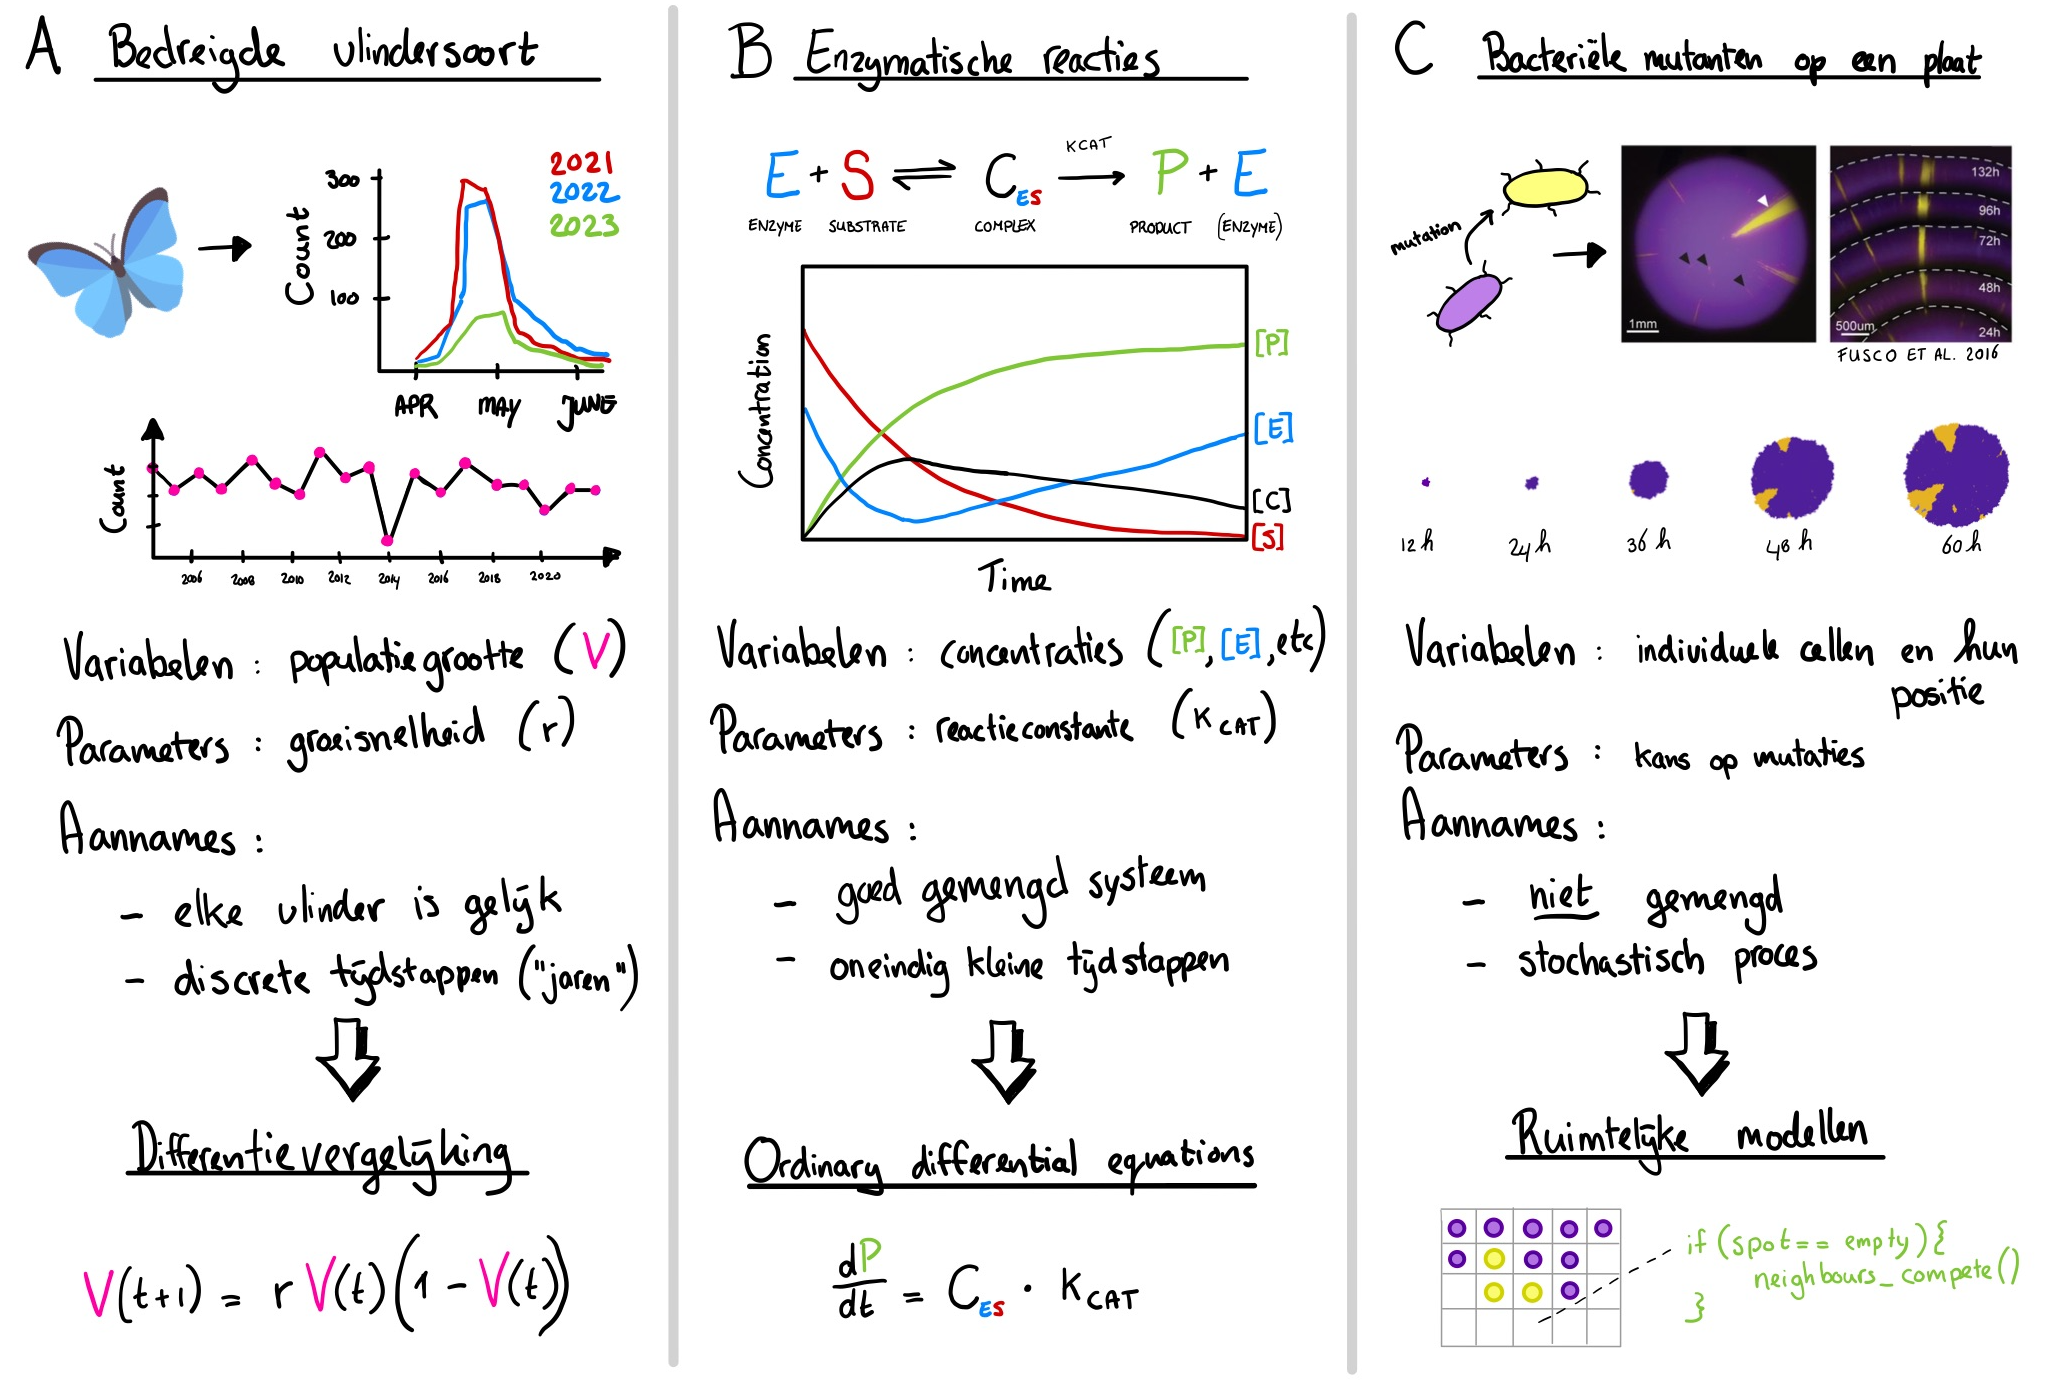
\includegraphics{Modellering/../Modellering/figuren/modeltypes.png}

}

\caption{\label{fig-modeltypes}Afhankelijk van het biologische scenario
kunnen we verschillende typen modellen gebruiken}

\end{figure}

Ondanks de eenvoud van differentievergelijkingen, werken we in de
biologie echter meestal met een ander type wiskundig model:
differen\emph{tiaal}vergelijkingen. In de literatuur zul je deze
modelvorm tegenkomen onder de noemer \emph{Ordinary Differential
Equations} (ODEs). Deze modellen omschrijven niet discrete tijdstappen
(jaar 1, jaar 2, \emph{etc}.), maar omschrijven in plaats daarvan
\textbf{de snelheid} waarmee de variabelen veranderen. Zo kun je
bijvoorbeeld chemische reactiesnelheden goed beschrijven met ODEs, en op
die manier bestuderen hoe enzymkinetiek werkt
(Figuur~\ref{fig-modeltypes} B). Omdat veel biologische processen goed
uit te drukken zijn in termen van snelheden (groeisnelheid,
reactiesnelheid, toxine-productie), is dit type model erg populair om
simpele biologische processen te modelleren. Daarom gaan we in deze
cursus uitgebreid bespreken hoe je dit type model kan lezen, en hoe je
er biologische conclusie uit kan trekken.

Hoewel ODEs populair zijn binnen de biologie, is er in de laatste jaren
steeds meer aandacht gekomen voor ruimtelijke patronen (\emph{spatial
patterns}). Wat hebben bijvoorbeeld de strepen van een zebravis te maken
met de patronen van struikgewassen op de toendra? Op het eerste gezicht
misschien niets, maar het blijkt dat beide patronen vormen door
hetzelfde mechanisme! Dergelijke patronen kunnen belangrijk zijn voor
natuurbehoud, en in het laatste hoofdstuk zal je zelfs zien dat er
belangrijke medische consequenties zijn. Het kan dus zeer nuttig zijn om
beter te begrijpen hoe patroon-vorming werkt. Hiervoor gebruiken we
ruimtelijke modellen (\emph{spatial models})
(Figuur~\ref{fig-modeltypes} C).

Aan het eind van dit cursusonderdeel zal je veel verschillende modellen
voorbij hebben zien komen: zowel simpele, wiskundige modellen zoals die
in Figuur~\ref{fig-modeltypes} A/B, als variaties op ruimtelijke
modellen zoals die in Figuur~\ref{fig-modeltypes} C. Het overkoepelende
doel is dat je basiskennis hebt over deze modellen, begrijpt waarom ze
belangrijk zijn binnen de biologie, en dat je kan je uitleggen welk
biologisch scenario het beste past bij welk type model.

\begin{exercise}[Modeluitkomsten]\protect\hypertarget{exr-modeluitkomsten}{}\label{exr-modeluitkomsten}

Elk type model heeft andere \emph{modeluitkomsten}: wiskundige modellen
hebben vaak vooral voorspellingen van veranderende aantallen, terwijl
ruimtelijke modellen ook patronen als resultaat hebben.

\textbf{a.} Waarom denk je dat een groeiende biofilm meestal niet met
ODEs wordt gemodelleerd? ANTWOORD: er is meer relevant dan alleen de
groeisnelheid

\textbf{b.} Waarom denk je dat een goed gemendge fles bacterien meestal
niet met een ruimtelijk model bestudeerd wordt? ANTWOORD: door goed te
mengen zijn de posities niet belangrijk, dus deze modelleren is niet
inzichtelijk

\textbf{c.} Waar zou je de vorming van korstmossen mee kunnen
modelleren? ANTWOORD: RUIMTELIJK MODEL

\end{exercise}

\hypertarget{wanneer-is-een-model-goed}{%
\section{Wanneer is een model
``goed''?}\label{wanneer-is-een-model-goed}}

Omdat modellen versimpelingen zijn, zullen ze nooit alle details uit de
biologie beschrijven. Dit is ook niet het doel van modellen. In plaats
daarvan proberen we, ondanks de versimpelingen, iets over biologie te
leren, of deze beter te voorspellen. Een model is daarom niet per se
slecht als het onrealistische aannames doet, omdat het best kan zijn dat
je er toch iets heel belangrijks van leert, of dat de voorspellingen
betrouwbaar zijn. De Britsche statisticus George P. Box zei ooit
hetvolgende over modellen:

\begin{quote}
\emph{``All models are wrong, but some are useful.''} -- George P. Box
\end{quote}

Als je nog niet helemaal begrijpt waarom zelfs onrealistische of
``foute'' modellen nuttig kunnen zijn, dan is dat niet erg. In dit
cursusonderdeel gaan we aan de hand van drie modules stapje voor stapje
leren werken met modellen, en je zult zien dat deze manier van denken
niet alleen heel nuttig, maar ook heel leuk kan zijn!

\hypertarget{terminologie}{%
\section{Terminologie}\label{terminologie}}

\begin{longtable}[]{@{}
  >{\raggedright\arraybackslash}p{(\columnwidth - 4\tabcolsep) * \real{0.2353}}
  >{\raggedright\arraybackslash}p{(\columnwidth - 4\tabcolsep) * \real{0.2353}}
  >{\raggedright\arraybackslash}p{(\columnwidth - 4\tabcolsep) * \real{0.5294}}@{}}
\toprule\noalign{}
\begin{minipage}[b]{\linewidth}\raggedright
Nederlands
\end{minipage} & \begin{minipage}[b]{\linewidth}\raggedright
Engels
\end{minipage} & \begin{minipage}[b]{\linewidth}\raggedright
Beschrijving
\end{minipage} \\
\midrule\noalign{}
\endhead
\bottomrule\noalign{}
\endlastfoot
Model & Model & Een versimpeling van een systeem, bijvoorbeeld in de
vorm van eenvoudige wiskunde of computerprogramma's \\
Dynamiek & Dynamics & Hoe dingen (variabelen) veranderen. Meestal zijn
we geinteresseerd in veranderingen over de tijd, maar soms ook in
veranderingen over de ruimte \\
Variabele & Variable & Wat er verandert, bijvoorbeeld het aantal
bacteriën tijdens exponentiële groei \\
Parameter & Parameter & Constante waardes die de dynamiek bepalen,
bijvoorbeeld de verdubbelingstijd van bacteriën \\
\end{longtable}

\hypertarget{sec-exp}{%
\chapter{Exponentiële groei}\label{sec-exp}}

\hypertarget{leerdoelen-1}{%
\section{Leerdoelen}\label{leerdoelen-1}}

In dit eerste hoofdstuk van Module 1 gaan we een belangrijk concept uit
de biologie beter leren begrijpen: exponentiële groei. Aan het eind van
dit onderdeel, word je geacht het volgende te kunnen:

\begin{itemize}
\tightlist
\item
  Aantonen wanneer groei exponentieel is
\item
  Uitleggen dat snelle groei niet altijd exponentiële groei is
\item
  Uitleggen wat dichtheidsafhankelijkheid (\emph{density dependence})
  is, en hoe dit resulteert in een draagvermogen (\emph{carrying
  capacity})
\end{itemize}

\begin{figure}

{\centering 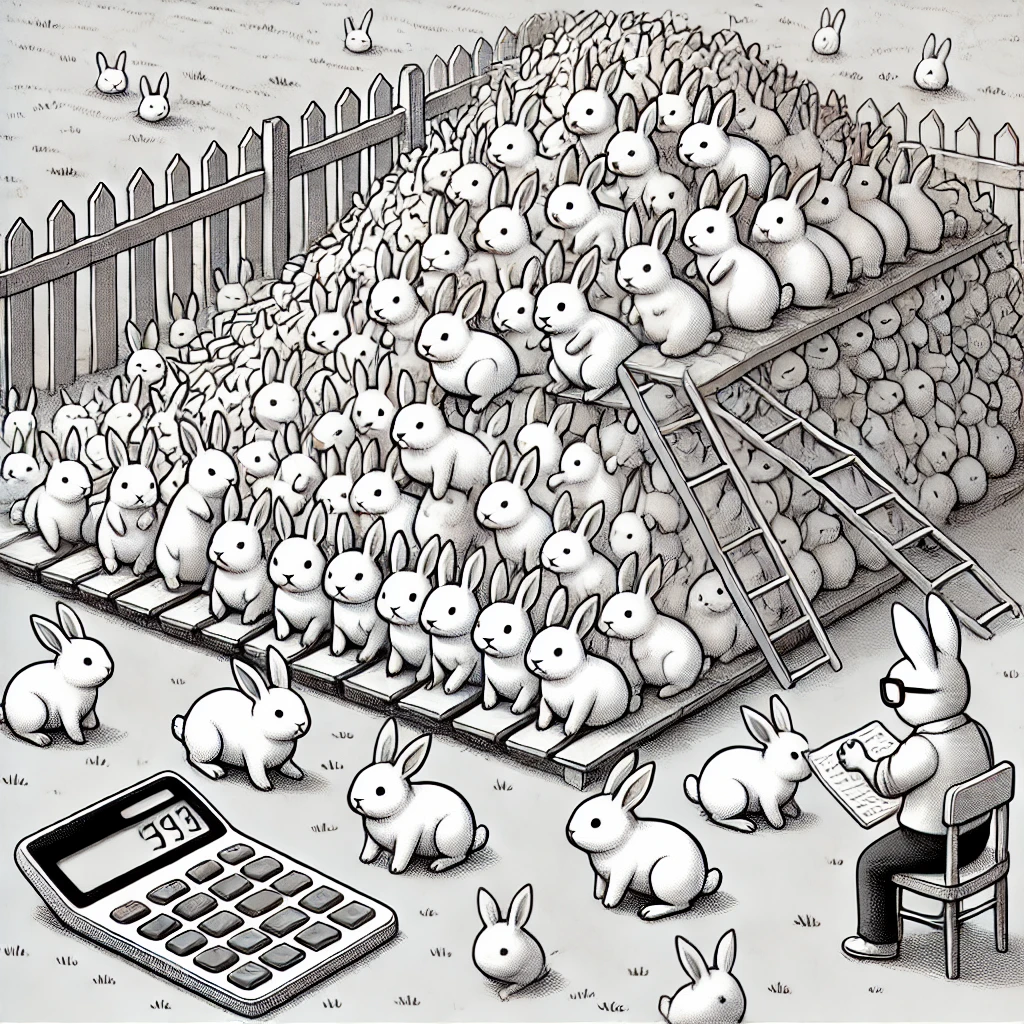
\includegraphics[width=0.8\textwidth,height=\textheight]{Modellering/../Modellering/figuren/knijnen.png}

}

\end{figure}

\hypertarget{bergen-met-rijst}{%
\section{Bergen met rijst}\label{bergen-met-rijst}}

In het introductie-hoofdstuk hebben we besproken dat alle modellen drie
belangrijke basisingrediënten hebben: variabelen, parameters, en
aannames. Laten we dit toepassen op een beroemde mythe over de
ontdekking van het schaakspel, waar een koning per ongeluk een beetje te
veel rijst beloofde.

\hypertarget{de-mythe-van-de-ontdekking-van-het-schaakspel}{%
\subsection{De mythe van de ontdekking van het
schaakspel}\label{de-mythe-van-de-ontdekking-van-het-schaakspel}}

De mythe van de ontdekking van het schaakspel is een beroemde legende
uit India. Volgens het verhaal wilde een koning de uitvinder van het
schaakspel belonen. De uitvinder vroeg bescheiden om rijst: één korrel
op het eerste veld van het schaakbord, twee op het tweede, vier op het
derde, en zo verder, telkens verdubbelend op elk van de 64 velden. De
koning stemde toe, zich niet realiserend hoeveel rijst dit zou
betekenen. Tegen de tijd dat het 64e veld bereikt was, had de koning
niet genoeg rijst in zijn hele koninkrijk om aan de vraag te voldoen.
Het totaal aantal korrels rijst komt uit op:

\[
1 + 2 + 4 + · · · + 26^3 = 26^4 − 1 = 18.446.744.073.709.551.615
\] Als je het aantal cijfers van dit grote getal telt, zie je dat het
neerkomt op 18 miljoen-miljoen-miljoen (een 18 met 18 nullen!). Dit
kunnen we beter als een macht van 10 schrijven:
\(\sim 1.84 \cdot 10^{19}\). In R worden dergelijke grote getallen
meestal met \texttt{e+} aangegeven:

\begin{Shaded}
\begin{Highlighting}[]
\DecValTok{2}\SpecialCharTok{\^{}}\DecValTok{64}
\end{Highlighting}
\end{Shaded}

\begin{Shaded}
\begin{Highlighting}[]
\NormalTok{[1] 1.844674e+19}
\end{Highlighting}
\end{Shaded}

Deze legende van de ontdekking van het schaakspel illustreert de kracht
van exponentiële groei en hoe snel getallen kunnen oplopen. Wat
aanvankelijk klein en bescheiden lijkt, kan snel uitgroeien tot een
enorme (onvoorstelbare) hoeveelheid.

\hypertarget{verdubellingen-modelleren}{%
\section{Verdubellingen modelleren}\label{verdubellingen-modelleren}}

De vergissing van de koning was dat hij (zoals veel mensen) niet in kon
zien hoe snel verdubbelingen toenemen. We kunnen deze aan de hand van
deze mythe de volgende variabelen, parameters, en aannames formuleren:

\begin{itemize}
\tightlist
\item
  Variabele: aantal rijstkorrels, 𝑅
\item
  Parameters: vermenigvuldigingswaarde (𝑟 = 2) en aantal hokjes op een
  schaakbord (\(n=64\))
\item
  Aannames: teveel om te benoemen, maar één is in ieder geval dat de
  rijst ook daadwerkelijk op het bord past!
\end{itemize}

Naast deze drie basisingrediënten, is het natuurlijk ook belangrijk om
te bepalen wat de hoeveelheid rijst is waar we mee beginnen (hier
\(R(0) = 1\)). Dit wordt in de model-wereld de \textbf{initiële
conditie} (\emph{initial condition}) genoemd. Vanaf daar gaan we verder
rekenen: op het tweede vakje liggen \(R(1) = R(0) \cdot 2\)
rijstkorrels, op het derde vakje \(R(2) = R(0) \cdot 2 \cdot 2\)
korrels, \emph{etc.} Het aantal korrels op het 64e vakje, wordt gegeven
door 63 verdubbelingen (het eerste vakje was al bezet!). Dit kunnen we
omschrijven met de volgende vergelijking:

\begin{equation}\protect\hypertarget{eq-rijst}{}{
R(63) = R(0) \cdot 2^{63}
}\label{eq-rijst}\end{equation}

Vergelijking Vergelijking~\ref{eq-rijst} geeft het aantal korrels op het
64e vakje. Dat is dus nog niet het \emph{totaal} aantal korrels. Het
totaal wordt gegeven door \(R(0) + R(1) + R(2) + \cdots + R(63)\). Deze
som is een beetje te lang om volledig op te schrijven, maar we weten dat
elke stap de volgende \textbf{differentievergelijking} wordt toegepast:

\begin{equation}\protect\hypertarget{eq-differentie-vergelijking}{}{
R(t+1) = 2\cdot R(t) 
}\label{eq-differentie-vergelijking}\end{equation}

We kunnen in R een simpele loop schrijven die vergelijking
Vergelijking~\ref{eq-differentie-vergelijking} herhaaldelijk toepast:

\begin{Shaded}
\begin{Highlighting}[]
\NormalTok{R }\OtherTok{\textless{}{-}} \DecValTok{1} \CommentTok{\# beginaantal rijst (initiële conditie)}

\CommentTok{\# herhaal iets 63 keer met een for{-}loop}
\ControlFlowTok{for}\NormalTok{ (t }\ControlFlowTok{in} \DecValTok{1}\SpecialCharTok{:}\DecValTok{63}\NormalTok{) \{}
\NormalTok{  R[t}\SpecialCharTok{+}\DecValTok{1}\NormalTok{] }\OtherTok{\textless{}{-}} \DecValTok{2}\SpecialCharTok{*}\NormalTok{R[t]}
\NormalTok{\}}
\FunctionTok{print}\NormalTok{(R[}\DecValTok{64}\NormalTok{])}
\end{Highlighting}
\end{Shaded}

\begin{verbatim}
[1] 9.223372e+18
\end{verbatim}

In de bovenstaande code wordt er steeds een getalletje aan R toegevoegd.
\(R\) is dus nu niet meer één getal, maar een steeds langer wordende
lijst getallen: \(1, 2, 4, 8, \dots, 2^{63}\) etcetera. Deze lijst
kunnen we zelf weer plotten met R:

\begin{Shaded}
\begin{Highlighting}[]
\CommentTok{\# beginaantal rijst}
\NormalTok{R }\OtherTok{\textless{}{-}} \DecValTok{1}

\CommentTok{\# herhaal iets 63 keer met een for{-}loop}
\ControlFlowTok{for}\NormalTok{ (i }\ControlFlowTok{in} \DecValTok{1}\SpecialCharTok{:}\DecValTok{63}\NormalTok{) \{}
\NormalTok{  R[i}\SpecialCharTok{+}\DecValTok{1}\NormalTok{] }\OtherTok{\textless{}{-}}\NormalTok{ R[i]}\SpecialCharTok{*}\DecValTok{2} \CommentTok{\# R in volgende stap is 2*R in deze stap}
\NormalTok{\}}

\FunctionTok{plot}\NormalTok{(R , }\AttributeTok{type=}\StringTok{\textquotesingle{}l\textquotesingle{}}\NormalTok{, }\AttributeTok{col=}\StringTok{"seagreen"}\NormalTok{, }\AttributeTok{log=}\StringTok{"y"}\NormalTok{, }\AttributeTok{lwd=}\DecValTok{2}\NormalTok{) }
\end{Highlighting}
\end{Shaded}

\begin{figure}[H]

{\centering 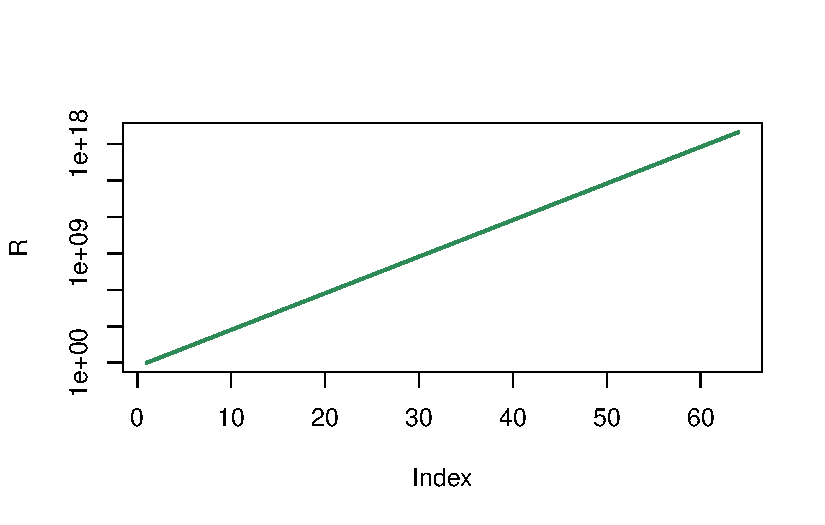
\includegraphics{Modellering/groei_exponentieel_files/figure-pdf/fig-exponential-1.pdf}

}

\caption{\label{fig-exponential}Het aantal rijstkorrels per vakje (met
log-lineaire schaal op de y-as).}

\end{figure}

\begin{exercise}[Een toenname van slechts
5\%]\protect\hypertarget{exr-exponentiele-groei-langzaam}{}\label{exr-exponentiele-groei-langzaam}

We plotten het resultaat van de loop hierboven op een log-lineaire
schaal (zie Hoofdstuk~\ref{sec-exponenten}), zodat we goed kunnen zien
of de groei exponentiëel is. Laten we nu aannemen dat de groei van het
aantal rijstkorrels niet verdubbelt, maar met 5 procent toeneemt per
hokje:

\[R(t+1) = 1.05 \cdot R(t)\] Pas de R-code hierboven aan om deze nieuwe
differentievergelijking door te rekenen.

\textbf{a.} Is er sprake van exponentiele groei?

\textbf{b.} Hoeveel rijstkorrels heb je nu in totaal? (hint: je kan de
\texttt{sum} functie gebruiken om de som van een vector in één keer uit
te rekenen!)

\end{exercise}

\hypertarget{exponentiuxeble-groei}{%
\section{Exponentiële groei}\label{exponentiuxeble-groei}}

Hoewel in het dagelijks taalgebruik elke vorm van ``snelle groei'' als
exponentieel wordt bestempeld, is dit niet correct. Hele snelle groei
kan niet exponentieel zijn, en andersom, kan vrij langzame groei wél
exponentieel zijn. Er is sprake van exponentiële groei als de
percentuele toename constant blijft. In de bovenstaande voorbeelden
waren dat een toename van 100\% (een verdubbeling) en een toename van
5\%, maar in beide gevallen was de toename constant. In beide gevallen
is er dus sprake van exponentiële groei! Als je zeker wil weten of groei
exponentiëel is, kun je data altijd plotten op een log-lineaire schaal
(\texttt{log="y"}), en kijken of het een rechte lijn vormt.

\hypertarget{konijnen-in-australiuxeb}{%
\section{Konijnen in Australië}\label{konijnen-in-australiuxeb}}

\begin{figure}

{\centering 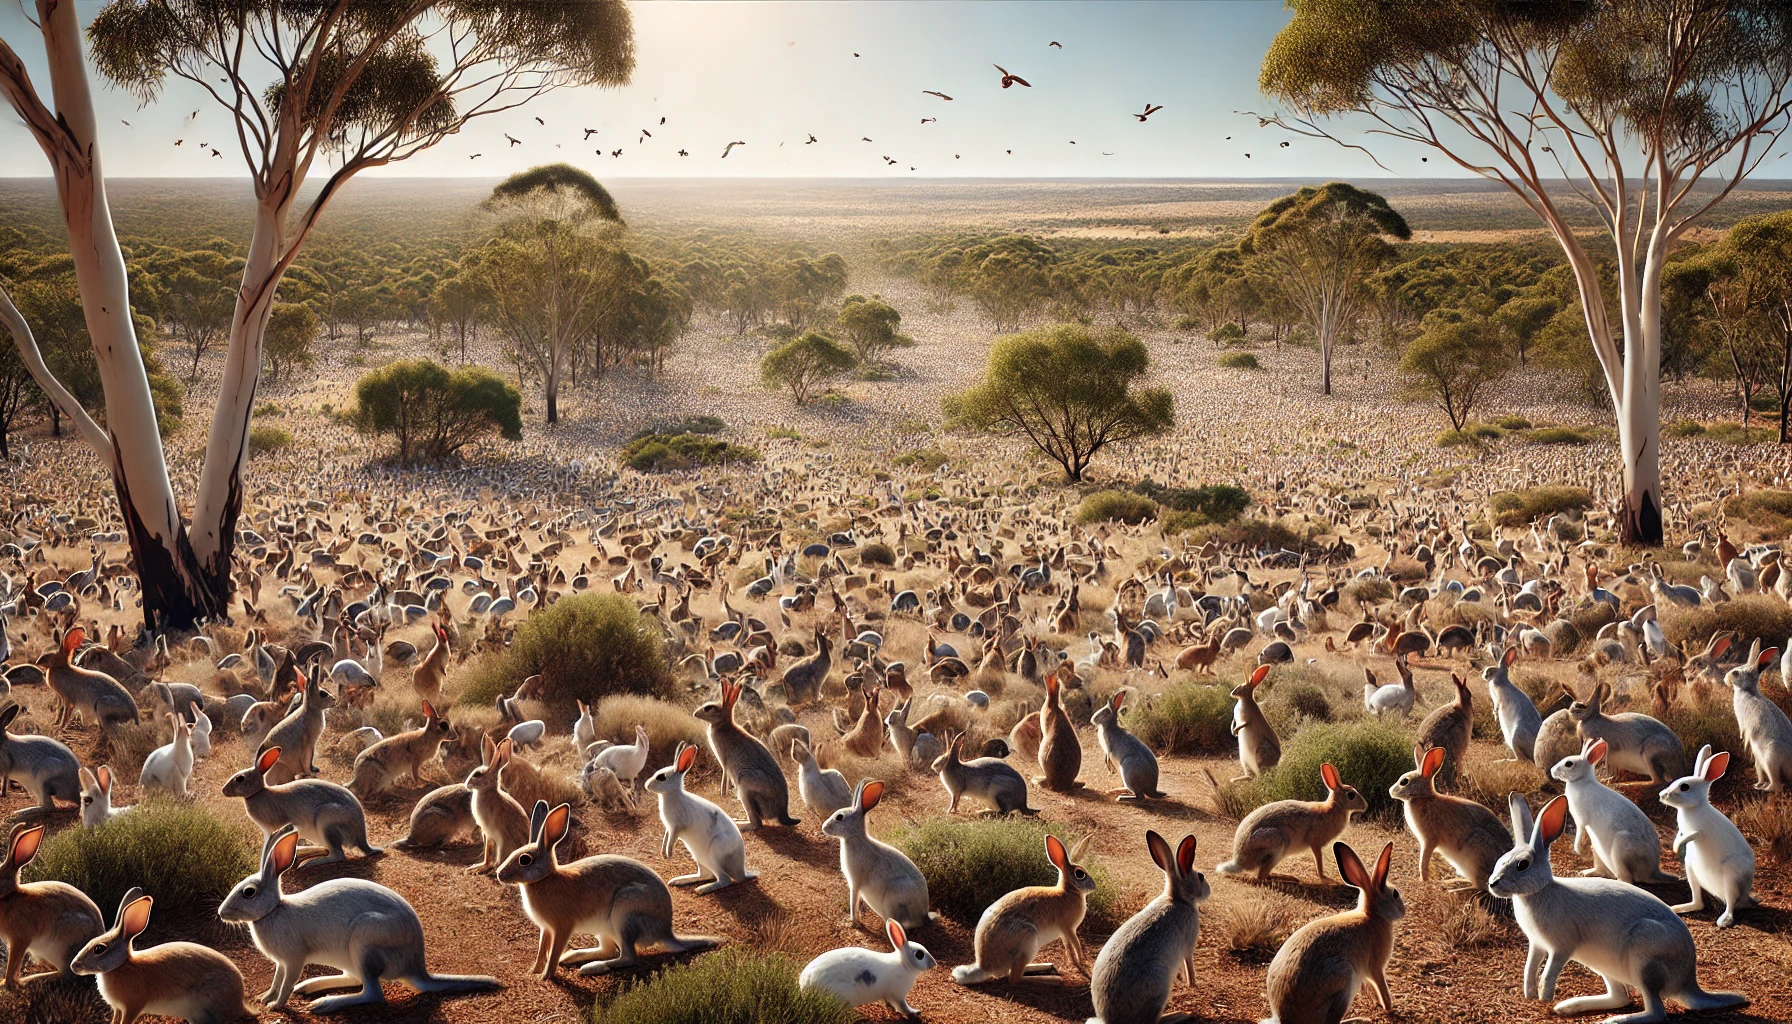
\includegraphics[width=0.8\textwidth,height=\textheight]{Modellering/../Modellering/figuren/konijnen_in_australie.png}

}

\end{figure}

Thomas Austin was een Engelse kolonist in Australië, en hield van jagen.
Daarom liet hij in de 19e eeuw 24 konijnen vrij in Autralië. Binnen tien
jaar waren er meer dan honderd miljoen konijnen op Australië, en kon de
populatie onmogelijk nog onder controle gehouden worden. Net als bij het
voorbeeld van de rijstkorrels, kunnen we een simpele
differentievergelijking opschrijven om het aantal konijnen in Autralië
te modelleren:

\begin{equation}
    N(t+1) = r \cdot N(t)
\end{equation}

N staat hier voor het aantal konijnen. In plaats van het getal
\texttt{2} of \texttt{1.05} in te vullen voor de groeisnelheid,
gebruiken we hier \(r\): een vrije parameter waarvan we de waarde nog
niet vastzetten. Zodoende kunnen we straks zelf bepalen of we \(r\) op
2, 3, of misschien nog wel hoger moeten zetten om de toenname in
Australië te kunnen verklaren.

\hypertarget{dichtheidseffecten-en-logistische-groei}{%
\section{Dichtheidseffecten en logistische
groei}\label{dichtheidseffecten-en-logistische-groei}}

Hoewel de groei van populaties aanvankelijk goed benaderd kan worden met
exponentiële groei, kan dit niet tot in het oneindige doorgaan. Zo kan
na verloop van tijd het eten opraken (voedsel is de beperkende factor),
of kan een graszaadje geen onbezet plekje in het veld meer vinden
(ruimte is de beperkende factor). Met andere woorden: hoe meer
individuen er aanwezig zijn, hoe minder groei er kan plaatsvinden.
Dergelijke effecten noemen we dichtheidseffecten, of
dichtheidsafhankelijkheid (\emph{density dependency}). De bovengenoemde
dichtheidseffecten zijn negatief (groei neemt af), maar
dichtheidseffecten kunnen ook positief zijn, bijvoorbeeld wanneer
individuen van een soort elkaar helpen met groeien, waar we later in
Hoofdstuk~\ref{sec-ruimtelijk} op terug zullen komen.

We gaan echter eerst onze pijlen richten op negatieve
dichtheidseffecten, omdat deze ons kunnen helpen om exponentiële groei
om te zetten naar \textbf{logistische groei}: groei die exponentiëel
begint maar uiteindelijk een stabiel evenwicht bereikt.

\begin{tcolorbox}[enhanced jigsaw, coltitle=black, breakable, bottomtitle=1mm, opacityback=0, colback=white, rightrule=.15mm, title=\textcolor{quarto-callout-note-color}{\faInfo}\hspace{0.5em}{Logaritmische groei}, bottomrule=.15mm, toprule=.15mm, left=2mm, colframe=quarto-callout-note-color-frame, toptitle=1mm, opacitybacktitle=0.6, titlerule=0mm, colbacktitle=quarto-callout-note-color!10!white, leftrule=.75mm, arc=.35mm]

Logistische groei is een vorm van populatiegroei die exponentieel
begint, maar uiteindelijk een evenwicht bereikt. Dit geeft de
karakteristieke sigmoïde S-curve. Op een log-lineaire schaal begint de
groeicurve als een rechte lijn, maar buigt deze uiteindelijk af naar een
evenwicht (Figuur~\ref{fig-logaritmischecurves}). Deze evenwichtswaarde
wordt ook wel de draagkracht of het \textbf{draagvermogen}
(\emph{carrying capacity}) van het systeem genoemd. Als de populatie
kleiner is dan dit draagvermogen (er zijn weinig konijnen dus veel
eten), dan zal de populatie toenemen. Is de populatie echter groter dan
dit draagvermogen (er zijn veel konijnen dus weinig eten), dan zal de
populatie alleen maar afnemen. Ergens daartussenin zal dus een
evenwichtsituatie liggen.

In de opgaven gaan we rekenen aan de konijnenpopulatie in Australië en
onze eerste poging doen om de populatie een stabiel evenwicht te laten
bereiken.

\begin{figure}[H]

{\centering 

\begin{Shaded}
\begin{Highlighting}[]
\NormalTok{x}\OtherTok{\textless{}{-}} \DecValTok{24}
\ControlFlowTok{for}\NormalTok{(i }\ControlFlowTok{in} \DecValTok{1}\SpecialCharTok{:}\DecValTok{70}\NormalTok{)\{}
\NormalTok{  x[i}\SpecialCharTok{+}\DecValTok{1}\NormalTok{] }\OtherTok{\textless{}{-}}\NormalTok{ x[i] }\SpecialCharTok{*} \FloatTok{1.2} \SpecialCharTok{*}\NormalTok{ (}\DecValTok{1}\SpecialCharTok{{-}}\NormalTok{(x[i]}\SpecialCharTok{/}\DecValTok{10}\SpecialCharTok{\^{}}\DecValTok{5}\NormalTok{))}
\NormalTok{\}}
\FunctionTok{par}\NormalTok{(}\AttributeTok{mfrow=}\FunctionTok{c}\NormalTok{(}\DecValTok{1}\NormalTok{,}\DecValTok{2}\NormalTok{))}
\FunctionTok{plot}\NormalTok{(x, }\AttributeTok{xlab=}\StringTok{"Tijd"}\NormalTok{, }\AttributeTok{ylab=}\StringTok{"Aantal"}\NormalTok{, }\AttributeTok{lwd=}\FloatTok{2.5}\NormalTok{, }\AttributeTok{type=}\StringTok{\textquotesingle{}l\textquotesingle{}}\NormalTok{, }\AttributeTok{col=}\StringTok{\textquotesingle{}seagreen\textquotesingle{}}\NormalTok{)}
\FunctionTok{plot}\NormalTok{(x, }\AttributeTok{xlab=}\StringTok{"Tijd"}\NormalTok{, }\AttributeTok{ylab=}\StringTok{"Aantal"}\NormalTok{, }\AttributeTok{lwd=}\FloatTok{2.5}\NormalTok{, }\AttributeTok{type=}\StringTok{\textquotesingle{}l\textquotesingle{}}\NormalTok{, }\AttributeTok{col=}\StringTok{\textquotesingle{}seagreen\textquotesingle{}}\NormalTok{,}\AttributeTok{log=}\StringTok{"y"}\NormalTok{)}
\end{Highlighting}
\end{Shaded}

\begin{figure}[H]

{\centering 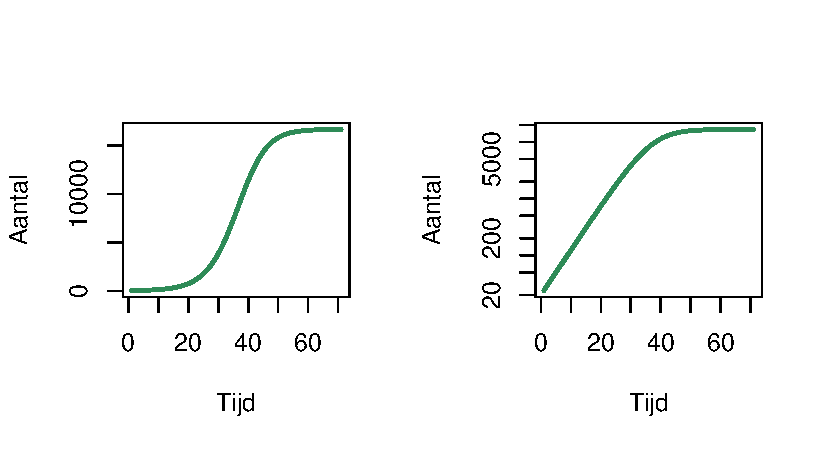
\includegraphics{Modellering/groei_exponentieel_files/figure-pdf/fig-logaritmischecurves-1.pdf}

}

\caption{Op lineaire schaal.}

\end{figure}

}

\caption{\label{fig-logaritmischecurves}Logistische groei.}

\end{figure}

\end{tcolorbox}

\hypertarget{opgaven}{%
\section{Opgaven}\label{opgaven}}

\begin{exercise}[Konijnen in
Australië]\protect\hypertarget{exr-rabbits-map}{}\label{exr-rabbits-map}

Als een biologische populatie zich ergens vestigt, kan het aanvankelijk
enorm snel groeien. Voorbeelden hiervan zijn een virus dat zich
verspreidt in een nieuwe gastheer, een bacteriële populatie in een
voedselrijk medium, of zoals in dit hoofdstuk omschreven, de
konijnenpopulatie in Australie:

\[
N(t+1) = r \cdot N(t) 
\] Exponentiële groei is zo simpel dat het gemakkelijk te simuleren is
met de computer, bijvoorbeeld in R. Neem devolgende code over in
Rstudio:

\begin{Shaded}
\begin{Highlighting}[]
\CommentTok{\# definieren van begin aantal konijnen}
\NormalTok{konijnen }\OtherTok{\textless{}{-}} \DecValTok{24}

\CommentTok{\# verdubbel het aantal konijnen 10 keer}
\ControlFlowTok{for}\NormalTok{ (i }\ControlFlowTok{in} \DecValTok{1}\SpecialCharTok{:}\DecValTok{10}\NormalTok{)\{}
\NormalTok{    konijnen }\OtherTok{\textless{}{-}}\NormalTok{ konijnen}\SpecialCharTok{*}\DecValTok{2}
\NormalTok{\}}
\end{Highlighting}
\end{Shaded}

\textbf{a.} Pas de code aan om te bepalen hoeveel konijnen er na 20
verdubbelingen zijn. Voeg aan het eind van de code zelf een regel toe,
waardoor er hetvolgende geprint wordt:
\texttt{Het\ aantal\ konijnen\ na\ 20\ tijdstappen\ is\ gelijk\ aan\ 25165824}.

\textbf{b.} Om beter bij te kunnen houden hoeveel konijnen er zijn na
elke herhaling, kunnen we het aantal konijnen bijhouden in een lijst,
waar we elke herhaling het aantal konijnen op dat tijdpunt aan
toevoegen:

\begin{Shaded}
\begin{Highlighting}[]
\CommentTok{\# Stap 1: Stel begin{-}aantal konijnen in}
\NormalTok{konijnen }\OtherTok{\textless{}{-}} \DecValTok{24}

\CommentTok{\# Stap 2: Verdubbel het aantal konijnen 30 keer}
\ControlFlowTok{for}\NormalTok{ (t }\ControlFlowTok{in} \DecValTok{1}\SpecialCharTok{:}\DecValTok{30}\NormalTok{)\{}
\NormalTok{  konijnen[t}\SpecialCharTok{+}\DecValTok{1}\NormalTok{] }\OtherTok{\textless{}{-}} \DecValTok{2}\SpecialCharTok{*}\NormalTok{konijnen[t]}
\NormalTok{\}}

\CommentTok{\# Stap 3: Plot het resultaat}
\FunctionTok{plot}\NormalTok{(konijnen, }\AttributeTok{type=}\StringTok{\textquotesingle{}l\textquotesingle{}}\NormalTok{)}
\end{Highlighting}
\end{Shaded}

Voer de bovenstaande code uit en bekijk het resultaat. Groeit het aantal
konijnen exponentieel? Pas de R-code aan om dit te bevestigen.

\textbf{c.} Hoewel het aantal konijnen in Australië aanvankelijk
exponentieel groeide, is er uiteindelijk een evenwicht bereikt bij
ongeveer 500 miljoen konijnen. Om dit in onze R-simulatie te bereiken
hebben we dichtheidsafhankelijkheid (\emph{density dependence}) nodig.
Dat wil zeggen: we willen dat de populatie minder toeneemt naar mate er
meer konijnen zijn. Om dit voor elkaar te krijgen kunnen we simpele
wiskundige functies gebruiken.

Wanneer is \(f(x) = 1 - \frac{x}{100}\) gelijk aan nul?

Wanneer is \(f(x) = 1 - \frac{x}{1000}\) gelijk aan nul?

Wanneer is \(f(x) = 1 - \frac{x}{K}\) gelijk aan nul?

\textbf{d.} De \(x\) uit de bovenstaande functie zou voor het aantal
konijnen (\(N\)) kunnen staan. Dat zou betekenen dat bij kleine
aantallen konijnen de functie bijna gelijk is aan \(1\), maar bij grote
aantallen konijnen deze steeds kleiner wordt. Als we onze
groei-vergelijking vermenigvuldigen met deze nieuwe functie \(f(N)\),
zouden we de groei dus moeten kunnen stoppen:

\[
N(t+1) = r \cdot N(t) \cdot f(N)
\]

Omdat \(f(N)\) steeds kleiner wordt, zal de groeisnelheid beschreven met
de bovenstaande differentievergelijking dus afnemen naar mate er meer
konijnen zijn. Pas de R-code aan zodat het voldoet aan de bovenstaande
vergelijking. Kies voor \(f(N)=1-N/K\) een waarde \(K=10^9\), en
simuleer de konijnenpopulatie voor 30 jaar. Bij hoeveel konijnen
stabiliseert de populatie? \emph{ANTWOORD: 500 miljoen. Anders dan bij
ODEs is dat niet K (maar dat weten ze nog niet per se, misschien wel
goed om toe te lichten als extratje in het antwoordenmodel omdat ze hier
misschien LATER naar terugkijken)}

\textbf{e.} Plot het aantal konijnen op een log-lineaire schaal (voeg
\texttt{log="y"} toe). Groeit de populatie in de eerste jaren (bij
benadering) exponentieel? Groeit de populatie in de laatste jaren
exponentieel?

\textbf{f.} Neem aan dat elke tijdstap 1 jaar is. Hoeveel konijnen zijn
er in je nieuwe model na 10 jaar? Wat is er vreemd aan deze hoeveelheid?
\emph{ANTWOORD: konijnen{[}10{]} geeft 12287.85. Dit is ten eerste raar
want we hebben dus kennelijk halve konijnen.}

\textbf{g.} De konijnenpopulatie bereikte naar schatting binnen 10 jaar
een populatiegrootte van meer dan honderd miljoen. Als we dit
vergelijken met onze eigen resultaten uit de bovenstaande vraag, groeit
onze populatie dus te langzaam. Pas de R-code aan waardoor de
konijnenpopulatie ieder jaar ver\textbf{drie}voudigd, en simuleer
wederom 30 tijdstappen (30 ``jaar''). Gaat de konijnenpopulatie naar een
evenwicht? Heb je dit keer wel ongeveer 100 miljoen konijnen na 10 jaar?
\emph{ANTWOORD: het gaat de hele tijd heen en weer rond 700 miljoen, en
nee, je hebt nogsteeds niet snel genoege groei}

\textbf{h.} Probeer ook wat er gebeurt als de populatie ieder jaar
ver\textbf{vier}voudigd. Wat valt je op? Heb je nu 100-miljoen konijnen
in 10 jaar? \emph{ANTWOORD: het gaat nu helemaal raar doen (chaos), en
nog steeds groeien ze niet eens snel genoeg (je hebt 6 miljoen
konijnen)}

\end{exercise}

\begin{exercise}[Miniatuur
Australië]\protect\hypertarget{exr-rabbits-in-space}{}\label{exr-rabbits-in-space}

\begin{figure}

{\centering 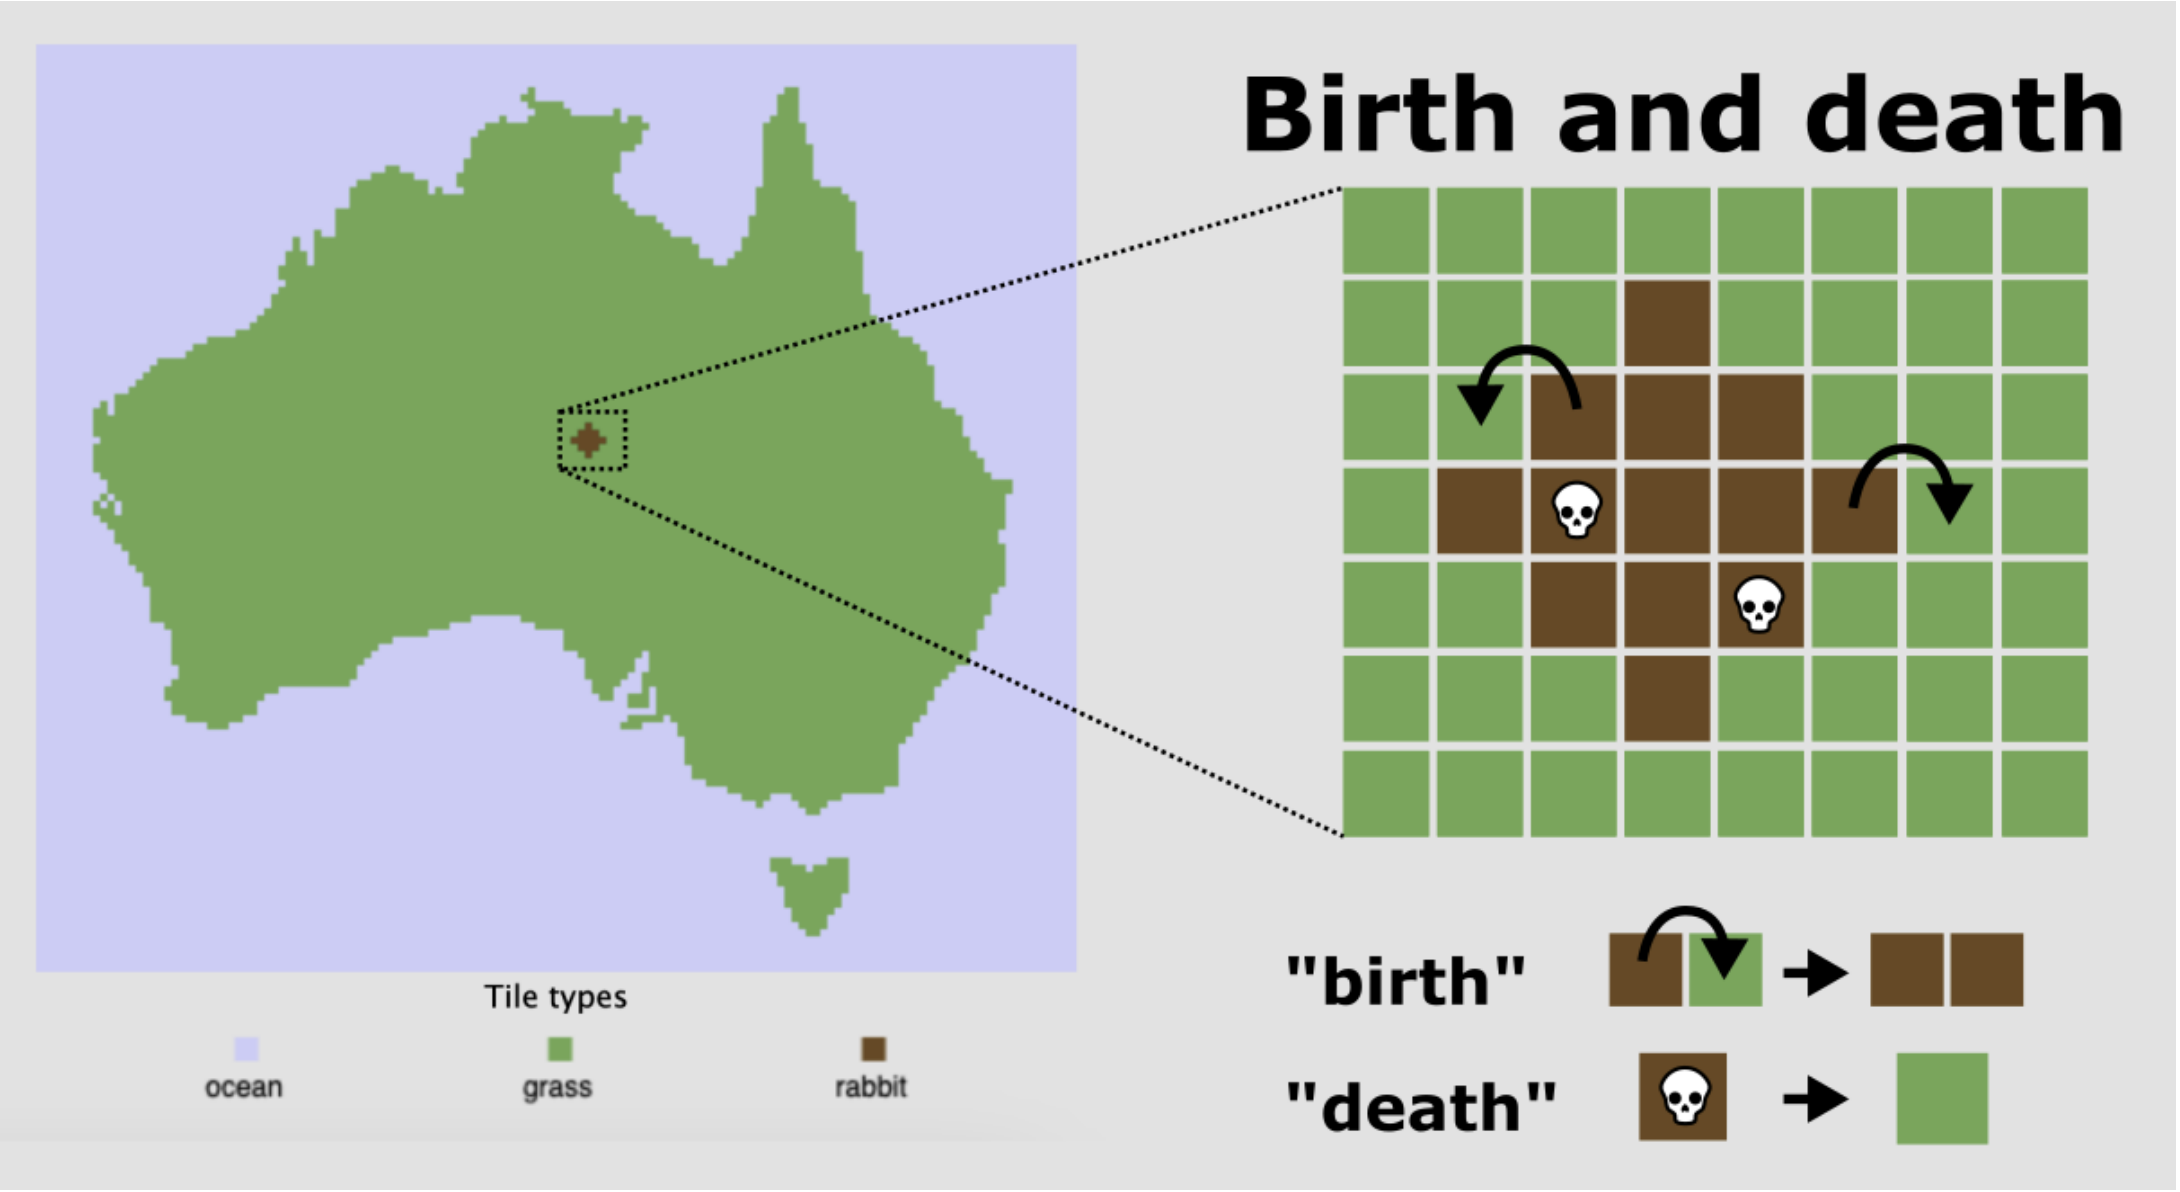
\includegraphics{Modellering/figuren/rabbits_in_australia.png}

}

\caption{\label{fig-rabbits-sim}\textbf{?(caption)}}

\end{figure}

Laten we de konijnenpopulatie uit de vorige opgave ook in een ander type
model bekijken. Hiervoor simuleren we een ``miniatuur Australië'' (zie
Figuur~\ref{fig-rabbits-sim}). Laten we Australië in drie types hokjes
opdelen: grashokjes (groen) waarop konijnen kunnen voortplanten,
konijnhokjes (bruin), en oceaanhokjes (blauw). We nemen voor het gemak
aan dat er geen woestijn-hokjes zijn, wat betekent dat konijnen overal
in Australie kunnen voortplanten. Elke tijdstap kunnen konijnen zich
vermenigvuldigen door een naastgelegen grashokje over te nemen. Deze
``geboortekans'' zetten we vast op 80\%, en ondervindt géén
dichtheidsafhankelijkheid. Konijnen kunnen ook met een vaste kans
sterven, waardoor een bruin hokje weer groen wordt. Als laatste nemen we
voor het gemak aan dat konijnen niet bewegen.

\begin{enumerate}
\def\labelenumi{\alph{enumi})}
\item
  Lees de bovenstaande modelomschrijving zorgvuldig door. Verwacht je
  exponentiële groei? Waarom wel/niet? \emph{ANTWOORD: naief verwacht je
  van wel, want b \textgreater{} d} \textbf{b.}
\item
  Verwacht je dat er een draagvlak (\emph{carrying capacity}) zal zijn?
  \emph{ANTWOORD: naief zou je denken van niet, want er is op het eerste
  gezicht geen afname van birth, maar misschien snappen ze ook wel dat
  dit niet kan!}
\item
  Een interactieve versie van deze simulatie zie je hieronder. Start de
  simulatie en bekijk de grafieken. Had je de vorige vragen juist
  beantwoord? \emph{ANTWOORD: misschien hadden ze geen draagvlak
  verwacht, maar achteraf gezien zullen ze zeker snappen dat dit wel
  MOET bestaan}
\end{enumerate}

\ldots{}

\begin{enumerate}
\def\labelenumi{\alph{enumi})}
\setcounter{enumi}{3}
\tightlist
\item
  De populatie groeit in het begin erg snel: 13, 100, 292, 619, 1081,
  1695, 2458, 3291. Bepaal met R of deze toename exponentieel is.
  \emph{ANTWOORD: nee, geeft geen rechte lijn op log-lin schaal:
  plot(c(13,100,292,619,1081,1695,2458,3191), log=``y'')}
\item
  De simulatie bereikt een draagvlak van ongeveer 8000 konijnen, wat
  veel minder is dan honderden miljoenen. We zouden een veel groter
  Australië kunnen simuleren, maar dat maakt een dergelijke
  computer-simulatie erg langzaam. We kunnen ook definiëren dat elk
  hokje niet 1 konijn is, maar een lokale populatie konijnen. Wat zou
  dit betekenen voor de interpretatie van de geboortekans en de
  sterftekans? \emph{ANTWOORD: dit zijn nu niet meer de geboorte /
  sterfte van individuen, maar de kans op uitbreiding / uitsterven van
  lokale populaties}
\end{enumerate}

\end{exercise}

\hypertarget{terminologie-1}{%
\section{Terminologie}\label{terminologie-1}}

\begin{longtable}[]{@{}
  >{\raggedright\arraybackslash}p{(\columnwidth - 4\tabcolsep) * \real{0.2466}}
  >{\raggedright\arraybackslash}p{(\columnwidth - 4\tabcolsep) * \real{0.2740}}
  >{\raggedright\arraybackslash}p{(\columnwidth - 4\tabcolsep) * \real{0.4795}}@{}}
\toprule\noalign{}
\begin{minipage}[b]{\linewidth}\raggedright
Nederlands
\end{minipage} & \begin{minipage}[b]{\linewidth}\raggedright
Engels
\end{minipage} & \begin{minipage}[b]{\linewidth}\raggedright
Beschrijving
\end{minipage} \\
\midrule\noalign{}
\endhead
\bottomrule\noalign{}
\endlastfoot
Initiele conditie & Initial condition & De begin-toestand van het model.
In simpele wiskundige modellen is dit vaak een aantal (zoals de
begin-hoeveelheid rijst in dit hoofdstuk). Bij andere modellen (uit
latere hoofdstukken) kan de begin-toestand kan ook een kleur of een
patroon zijn. \\
Differentievergelijking & Difference equation / Map & Een wiskundige
formule die de relatie beschrijft tussen opeenvolgende waarden van een
variabele in \textbf{discrete} tijdstappen \\
Exponentiële groei & Exponential growth & Groei waarbij het
toenamingspercentage constant blijft \\
Logaritmische groei & Logarithmic growth & Groei die exponentiëel
begint, maar wat uiteindelijk een evenwicht bereikt. \\
Draagvermogen & Carrying capacity & Het maximale aantal individuen (of
de maximale concentratie) dat een systeem in evenwicht kan
ondersteunen \\
\end{longtable}

\hypertarget{sec-odes}{%
\chapter{Modelleren met ODEs}\label{sec-odes}}

In dit onderdeel bouwen we voort op de kennis van exponentiële groei,
logistische groei, en draagvermogen, maar stappen we af van de
differentievergelijking. We gaan kennis maken met
differen\emph{tiaal}vergelijkingen (ordinary differential
equations/ODEs). ODEs zijn binnen de biologie -- en ook in andere
wetenschappen -- een zeer populaire manier om systemen te modelleren,
omdat ze relatief simpel en intuïtief zijn.

\hypertarget{leerdoelen-2}{%
\section{Leerdoelen}\label{leerdoelen-2}}

De leerdoelen voor dit hoofdstuk zijn:

\begin{itemize}
\tightlist
\item
  Begrijpen dat biologie modelleren met discrete tijdstappen soms
  vreemde (maar interessante!) effecten op kan leveren
\item
  Begrijpen dat ODEs geen ``tijdstappen'' hebben
\item
  Begrijpen dat ODEs geschreven worden in termen van ``x per
  tijdseenheid'', en wat dit zegt over de individuele termen en
  parameters
\item
  Begrijpen wanneer er in een ODE sprake is van een evenwicht
\item
  Het in verband kunnen brengen van ODEs en hun oplossing
\end{itemize}

\begin{figure}

{\centering 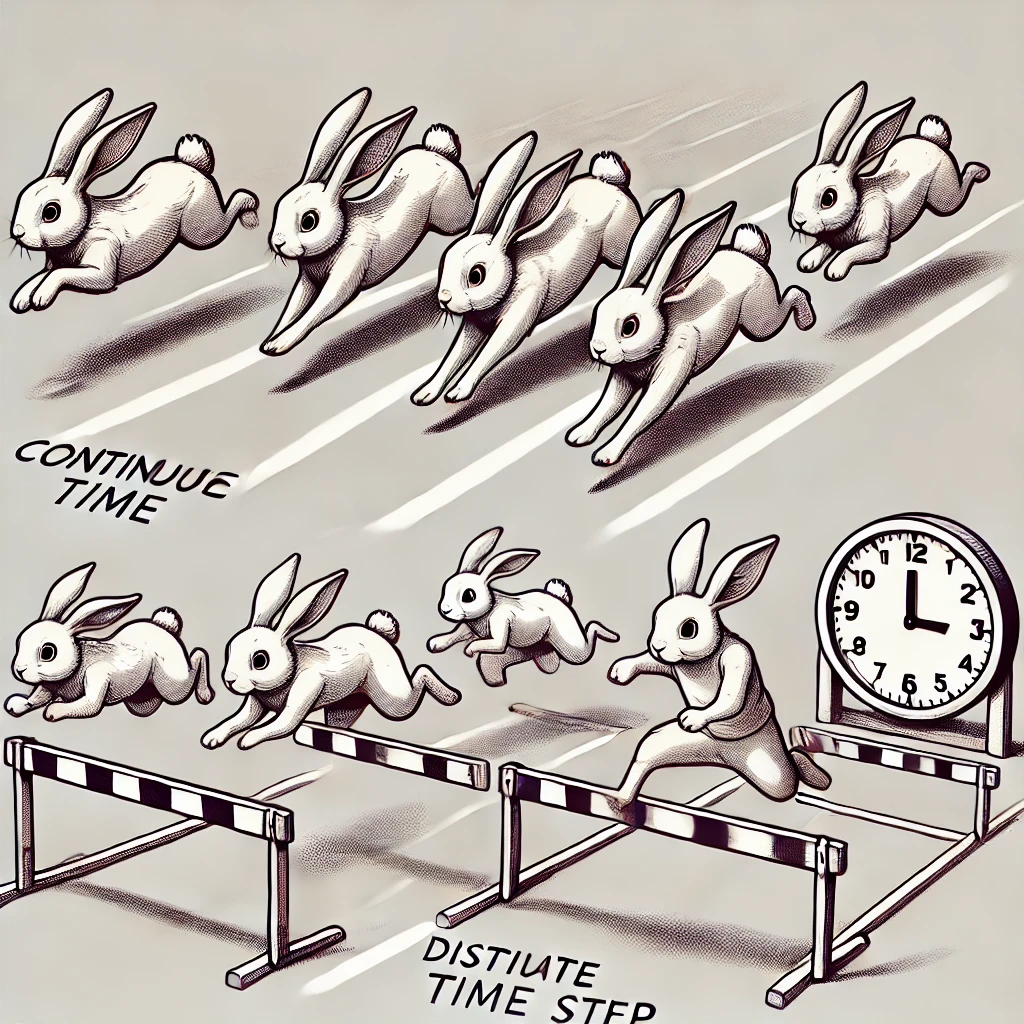
\includegraphics[width=0.8\textwidth,height=\textheight]{Modellering/../Modellering/figuren/discr_vs_cont_ai.png}

}

\caption{Afbeelding gegenereerd met ChatGPT4-o}

\end{figure}

\hypertarget{chaotische-konijnen}{%
\section{Chaotische konijnen}\label{chaotische-konijnen}}

In Hoofdstuk~\ref{sec-exp} hebben we gezien wat de consequenties zijn
van 24 konijnen vrijlaten in een land waar geen natuurlijke predator
voor konijnen bestaat. In de opgaven hebben we deze groei gemodelleerd
in R, en geprobeerd om de groei van deze konijnen enigszins te beperken
door een draagvermogen in te bouwen. Hoewel dit goed leek te gaan
wanneer de intrinsieke groeisnelheid (\(r\)) laag was, liet snellere
groei een vreemde grafieken zien (Figuur~\ref{fig-chaos-1}). Van het één
op het andere jaar springen we heen en weer van honderden miljoenen
konijnen naar een heel klein aantal konijnen, en dit gaat over de jaren
heen steeds maar door. Sterker nog, als we Thomas Austin's experiment
herhalen met een ander aantal konijnen (Figuur~\ref{fig-chaos-2}) zien
we dat deze fluctuaties iedere keer heel anders zijn! Met andere
woorden: als we met behulp van dit model zouden willen voorspellen
hoeveel konijnen er na 20 jaar zouden zijn, dan moeten we wel héél zeker
weten met hoeveel konijn we precies begonnen! Bovendien hebben we niet
bereikt wat we wilden: probeerde we niet juist een stabiel evenwicht te
modelleren?

\begin{figure}

\begin{minipage}[t]{0.50\linewidth}

{\centering 

\begin{Shaded}
\begin{Highlighting}[]
\FunctionTok{library}\NormalTok{(ggplot2)}
\FunctionTok{library}\NormalTok{(dplyr)}
\NormalTok{r }\OtherTok{=} \DecValTok{2}        \CommentTok{\# intrinsic growth rate}
\NormalTok{K }\OtherTok{=} \DecValTok{10}\SpecialCharTok{\^{}}\DecValTok{8}
\NormalTok{init\_R }\OtherTok{=} \DecValTok{24}    \CommentTok{\# start with 13}

\NormalTok{R\_series }\OtherTok{\textless{}{-}} \FunctionTok{data.frame}\NormalTok{()}
\ControlFlowTok{for}\NormalTok{(r }\ControlFlowTok{in} \FunctionTok{c}\NormalTok{(}\DecValTok{4}\NormalTok{))\{}
  \ControlFlowTok{for}\NormalTok{(s }\ControlFlowTok{in} \FunctionTok{c}\NormalTok{(}\DecValTok{24}\SpecialCharTok{:}\DecValTok{26}\NormalTok{))\{ }
\NormalTok{    R }\OtherTok{=}\NormalTok{ s}
\NormalTok{    myR }\OtherTok{=}\NormalTok{ R}
\NormalTok{    R\_series }\OtherTok{\textless{}{-}} \FunctionTok{rbind}\NormalTok{(R\_series, }\FunctionTok{data.frame}\NormalTok{(}\AttributeTok{time=}\DecValTok{0}\NormalTok{, }\AttributeTok{r=}\NormalTok{r, }\AttributeTok{R=}\NormalTok{R,}\AttributeTok{s=}\NormalTok{s,}\AttributeTok{initR=}\NormalTok{myR))}
    \ControlFlowTok{for}\NormalTok{(i }\ControlFlowTok{in} \DecValTok{1}\SpecialCharTok{:}\DecValTok{50}\NormalTok{)}
\NormalTok{    \{}
\NormalTok{      R }\OtherTok{\textless{}{-}}\NormalTok{ r}\SpecialCharTok{*}\NormalTok{R}\SpecialCharTok{*}\NormalTok{(}\DecValTok{1}\SpecialCharTok{{-}}\NormalTok{R}\SpecialCharTok{/}\NormalTok{K)}
\NormalTok{      R\_series }\OtherTok{\textless{}{-}} \FunctionTok{rbind}\NormalTok{(R\_series, }\FunctionTok{data.frame}\NormalTok{(}\AttributeTok{time=}\NormalTok{i,}\AttributeTok{r=}\NormalTok{r,}\AttributeTok{R=}\NormalTok{R,}\AttributeTok{s=}\NormalTok{s,}\AttributeTok{initR=}\NormalTok{myR))}
\NormalTok{    \}}
\NormalTok{  \}}
\NormalTok{\}}

\NormalTok{R\_series }\SpecialCharTok{\%\textgreater{}\%} \FunctionTok{filter}\NormalTok{(initR}\SpecialCharTok{==}\DecValTok{24}\NormalTok{,time}\SpecialCharTok{\textgreater{}}\DecValTok{1}\NormalTok{,time}\SpecialCharTok{\textless{}=}\DecValTok{40}\NormalTok{,r}\SpecialCharTok{==}\DecValTok{4}\NormalTok{) }\SpecialCharTok{\%\textgreater{}\%} 
  \FunctionTok{ggplot}\NormalTok{(}\FunctionTok{aes}\NormalTok{(}\AttributeTok{x=}\NormalTok{time,}\AttributeTok{y=}\NormalTok{R,}\AttributeTok{group=}\NormalTok{s,}\AttributeTok{col=}\FunctionTok{as.factor}\NormalTok{(initR))) }\SpecialCharTok{+} 
  \FunctionTok{geom\_line}\NormalTok{(}\AttributeTok{size=}\FloatTok{1.5}\NormalTok{) }\SpecialCharTok{+} 
  \CommentTok{\#facet\_wrap(\textasciitilde{}r, scale="free\_y",ncol=1) + }
  \FunctionTok{theme\_bw}\NormalTok{() }\SpecialCharTok{+}
  \FunctionTok{scale\_color\_brewer}\NormalTok{(}\AttributeTok{type=}\StringTok{"qual"}\NormalTok{, }\AttributeTok{palette =} \StringTok{"Dark2"}\NormalTok{, }\AttributeTok{name=}\StringTok{""}\NormalTok{) }\SpecialCharTok{+}
  \FunctionTok{guides}\NormalTok{(}\AttributeTok{color=}\StringTok{"none"}\NormalTok{)}\SpecialCharTok{+}
  \FunctionTok{ylab}\NormalTok{(}\StringTok{"Aantal konijnen"}\NormalTok{) }\SpecialCharTok{+}
  \FunctionTok{xlab}\NormalTok{(}\StringTok{"Tijd (jaren)"}\NormalTok{) }\SpecialCharTok{+}
  \FunctionTok{theme\_minimal}\NormalTok{(}\AttributeTok{base\_size=}\DecValTok{16}\NormalTok{)}\SpecialCharTok{+}
  \FunctionTok{theme}\NormalTok{(}\AttributeTok{plot.margin =} \FunctionTok{unit}\NormalTok{(}\FunctionTok{c}\NormalTok{(}\DecValTok{0}\NormalTok{,}\DecValTok{0}\NormalTok{,}\DecValTok{0}\NormalTok{,}\DecValTok{0}\NormalTok{), }\StringTok{"cm"}\NormalTok{))}
\end{Highlighting}
\end{Shaded}

\begin{figure}[H]

{\centering 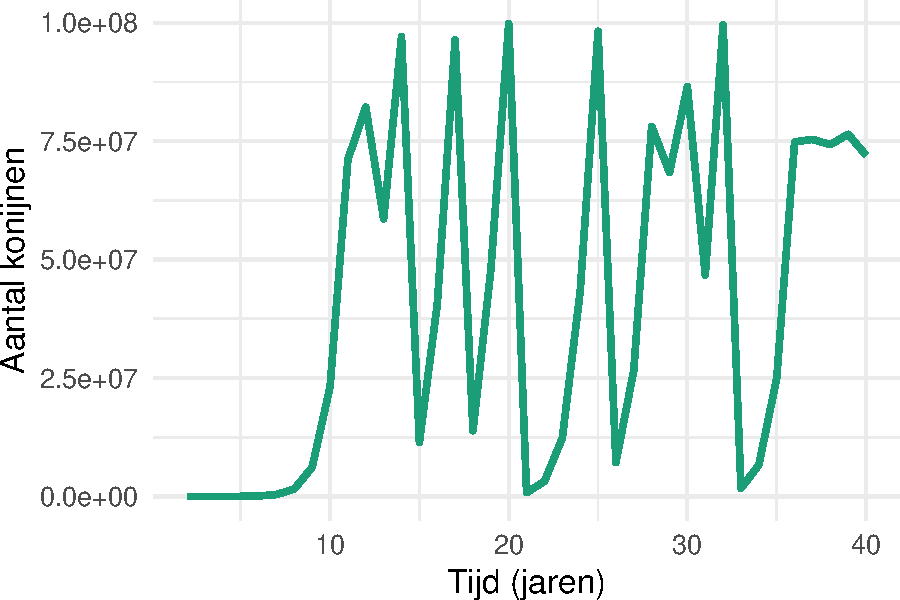
\includegraphics{Modellering/groei_odes_files/figure-pdf/fig-chaos-1-1.pdf}

}

\caption{Snel-groeiende populatie gemodelleerd met een
differentievergelijking, beginnende met 24 konijnen}

\end{figure}

}

\end{minipage}%
%
\begin{minipage}[t]{0.50\linewidth}

{\centering 

\begin{Shaded}
\begin{Highlighting}[]
\NormalTok{R\_series }\SpecialCharTok{\%\textgreater{}\%} \FunctionTok{filter}\NormalTok{(time}\SpecialCharTok{\textgreater{}}\DecValTok{1}\NormalTok{,time }\SpecialCharTok{\textless{}}\DecValTok{40}\NormalTok{,r}\SpecialCharTok{==}\DecValTok{4}\NormalTok{) }\SpecialCharTok{\%\textgreater{}\%} 
  \FunctionTok{ggplot}\NormalTok{(}\FunctionTok{aes}\NormalTok{(}\AttributeTok{x=}\NormalTok{time,}\AttributeTok{y=}\NormalTok{R,}\AttributeTok{group=}\NormalTok{s,}\AttributeTok{col=}\FunctionTok{as.factor}\NormalTok{(initR))) }\SpecialCharTok{+} 
  \FunctionTok{geom\_line}\NormalTok{(}\AttributeTok{size=}\FloatTok{1.2}\NormalTok{) }\SpecialCharTok{+} 
  \CommentTok{\#facet\_wrap(\textasciitilde{}r, scale="free\_y",ncol=1) + }
  \FunctionTok{theme\_bw}\NormalTok{() }\SpecialCharTok{+}
  \FunctionTok{guides}\NormalTok{(}\AttributeTok{color=}\StringTok{"none"}\NormalTok{)}\SpecialCharTok{+}
  \FunctionTok{scale\_color\_brewer}\NormalTok{(}\AttributeTok{type=}\StringTok{"qual"}\NormalTok{, }\AttributeTok{palette =} \StringTok{"Dark2"}\NormalTok{, }\AttributeTok{name=}\StringTok{"Begin aantal}\SpecialCharTok{\textbackslash{}n}\StringTok{konijnen"}\NormalTok{) }\SpecialCharTok{+}
  \FunctionTok{guides}\NormalTok{(}\AttributeTok{alpha=}\StringTok{"none"}\NormalTok{) }\SpecialCharTok{+}
  \FunctionTok{ylab}\NormalTok{(}\StringTok{"Aantal konijnen"}\NormalTok{) }\SpecialCharTok{+}
  \FunctionTok{xlab}\NormalTok{(}\StringTok{"Tijd (jaren)"}\NormalTok{) }\SpecialCharTok{+}
  \FunctionTok{theme\_minimal}\NormalTok{(}\AttributeTok{base\_size=}\DecValTok{16}\NormalTok{)}\SpecialCharTok{+}
  \FunctionTok{theme}\NormalTok{(}\AttributeTok{plot.margin =} \FunctionTok{unit}\NormalTok{(}\FunctionTok{c}\NormalTok{(}\DecValTok{0}\NormalTok{,}\DecValTok{0}\NormalTok{,}\DecValTok{0}\NormalTok{,}\DecValTok{0}\NormalTok{), }\StringTok{"cm"}\NormalTok{))}
\end{Highlighting}
\end{Shaded}

\begin{figure}[H]

{\centering 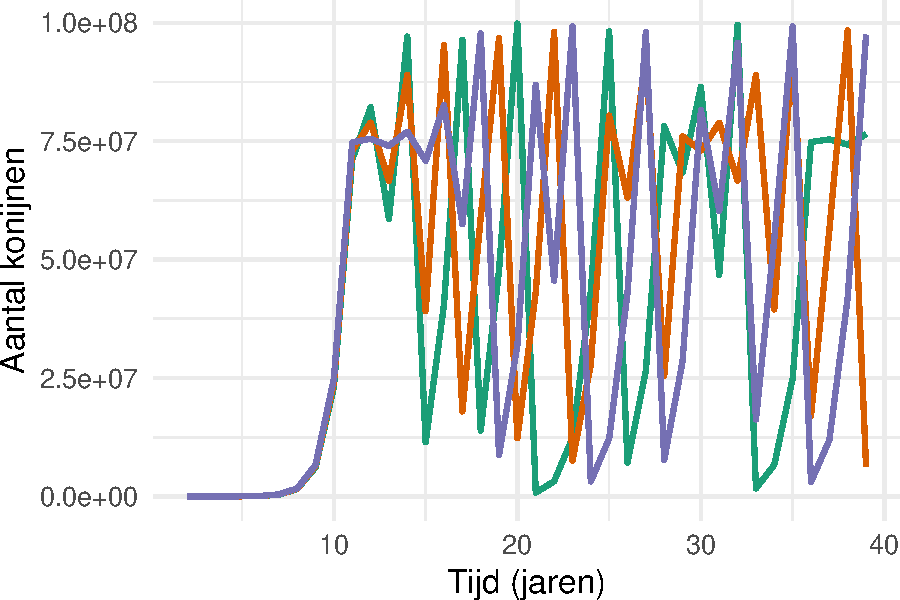
\includegraphics{Modellering/groei_odes_files/figure-pdf/fig-chaos-2-1.pdf}

}

\caption{Snel-groeiende populatie gemodelleerd met een
differentievergelijking, beginnende met 24 (groen), 25 (rood), en 26
(paars) konijnen}

\end{figure}

}

\end{minipage}%

\caption{\label{fig-chaos}\textbf{?(caption)}}

\end{figure}

Het vreemde gedrag in Figuur~\ref{fig-chaos} wordt formeel
\textbf{deterministische chaos} genoemd. Hiermee bedoelen we niet het
type chaos dat men in spreektaal gebruikt om een rommelige kamer te
omschrijven, maar de onvoorspelbare fluctuaties die bovendien extreem
gevoelig zijn voor de begin-toestand. Een andere beroemd voorbeeld uit
de natuurkunde is de
\href{https://nl.wikipedia.org/wiki/Dubbele_slinger}{dubbele slinger}.
Hoewel je op korte termijn vaak nog enigszins kan aanvoelen in welke
richting de slinger beweegt, is het op lange termijn onmogelijk in te
schatten waar de slinger zich zal bevinden. Kennelijk kunnen zelfs
simpele systemen zich enorm vreemd en onvoorspelbaar gedragen. Geen
wonder dat meer complexe systemen zoals biologische populaties en het
weer zo moeilijk te voorspellen zijn!

\begin{tcolorbox}[enhanced jigsaw, coltitle=black, breakable, bottomtitle=1mm, opacityback=0, colback=white, rightrule=.15mm, title=\textcolor{quarto-callout-tip-color}{\faLightbulb}\hspace{0.5em}{Meer over ``deterministische chaos'' (verdieping)}, bottomrule=.15mm, toprule=.15mm, left=2mm, colframe=quarto-callout-tip-color-frame, toptitle=1mm, opacitybacktitle=0.6, titlerule=0mm, colbacktitle=quarto-callout-tip-color!10!white, leftrule=.75mm, arc=.35mm]

Een systeem is deterministisch als de regels niet willekeurig zijn. Met
andere woorden, er worden geen dobbelstenen gerold om te bepalen wat er
gebeurt. De meeste chemische en biologische principes volgen zulke
deterministische regeltjes, maar toch zijn ze moeilijk te voorspellen.
Dit komt doordat ze ondanks het gebrek aan willekeur zeer gevoelig zijn
voor de precisie van de metingen. Deze gevoeligheid ken je misschien van
het concept the \emph{butterfly effect}, waar een vleugelslag van een
vlinder uiteindelijk (na lange tijd) de oorzaak kan zijn van een orkaan.
Dit wordt chaos genoemd. Zo zie je bijvoorbeeld dat als Thomas Austin 25
in plaats van 24 konijnen had vrijgelaten, dit een enorm ander beeld
schept.

\end{tcolorbox}

Hoewel deterministische chaos een interessant fenomeen is (en zeer zeker
niet zomaar ``willekeur'', zie (\textbf{tip-detchaos?})), kunnen we ons
afvragen of de groei van biologische populaties ook daadwerkelijk
chaotisch is. Als we bijvoorbeeld bacteriën in het lab groeien, krijgen
we meestal een logistische (sigmoïde) groeicurve, en niet een populatie
die lukraak fluctueert. Wat is nou eigenlijk de oorzaak van deze chaos,
en kunnen we hier misschien ook vanaf komen?

\hypertarget{het-probleem-van-tijdstappen}{%
\section{Het probleem van
``tijdstappen''}\label{het-probleem-van-tijdstappen}}

Tot nu toe namen we aan dat elke ``tijdstap'' van de konijnenpopulatie
een jaar is. Met een bepaalde groeisnelheid (\(r=2\)) geeft dit
inderdaad prachtige logischtische groei, maar de daadwerkelijke
populatie konijnen groeide sneller (dus: \(r>2\)). Helaas zagen we dat
het verhogen van \(r\) niet de gewenste resultaten heeft. Wat kunnen we
doen om toch ``snellere groei'' te krijgen?

We zouden kunnen overwegen om niet \(r\) aan te passen, maar in plaats
daarvan te heroverwegen wat ``een tijdstap'' is. Dat wil zeggen, hoeveel
tijd zit er eigenlijk tussen \(R(t)\) en \(R(t+1)\)? Als elke tijdstap
een half jaar is, is er na 20 tijdstappen slechts 10 jaar voorbij. Dat
betekent dat er nu na 10 jaar, 20 stappen groei hebben kunnen
plaatsvinden. Als elke tijdstap \(1 \over 10\) jaar is, is er na 20
tijdstappen pas 2 jaar voorbij. Na 10 jaar zullen er dus nog meer
groei-stappen hebben plaatsgevonden. Met andere woorden; de grootte van
de tijdstap kan ook beinvloeden hoe snel onze populatie konijnen groeit!

Om de grootte van onze tijdstap aan te passen, kunnen we ons R-script
uit de opgaven van het vorige onderdeel hergebruiken:

\begin{Shaded}
\begin{Highlighting}[]
\CommentTok{\# definieren van begin aantal konijnen}
\NormalTok{konijnen }\OtherTok{\textless{}{-}} \DecValTok{24}

\CommentTok{\# herhaal 40 keer de groei{-}vergelkijking, waarbij elke stap staat voor een HALF jaar}
\ControlFlowTok{for}\NormalTok{ (t }\ControlFlowTok{in} \DecValTok{1}\SpecialCharTok{:}\DecValTok{40}\NormalTok{)\{}
\NormalTok{  konijnen[t}\SpecialCharTok{+}\DecValTok{1}\NormalTok{] }\OtherTok{\textless{}{-}} \DecValTok{2}\SpecialCharTok{*}\NormalTok{konijnen[t]}\SpecialCharTok{*}\NormalTok{(}\DecValTok{1}\SpecialCharTok{{-}}\NormalTok{(konijnen[t]}\SpecialCharTok{/}\DecValTok{10}\SpecialCharTok{\^{}}\DecValTok{9}\NormalTok{))}
\NormalTok{\}}
\NormalTok{konijnen[}\DecValTok{20}\NormalTok{] }\CommentTok{\# Aantal na 20 halve jaren}
\FunctionTok{plot}\NormalTok{(konijnen,}\AttributeTok{type=}\StringTok{"o"}\NormalTok{,}\AttributeTok{xlab=}\StringTok{"Tijd"}\NormalTok{,}\AttributeTok{ylab=}\StringTok{"Aantal konijnen"}\NormalTok{)}
\end{Highlighting}
\end{Shaded}

Als je de code hierboven uitvoert zul je zien dat er na 20 halve jaren
12,425,902 konijnen zijn, en dat we gewoon een mooie sigmoïde groeicurve
krijgen. Dit is ook niet raar, want eigenlijk hebben we niets aangepast:
alleen onze intepretatie van ``tijd-stappen'' is anders. Door aan te
nemen dat de tijdstap kleiner is (een half jaar in plaats van een jaar),
zijn we het vreemde chaotische gedrag kwijt. Kennelijk ontstaat dit
probleem alleen als de tijdstap ``te groot'' is.

Dit kunnen we ook intuïtief begrijpen. Als je alleen kijkt naar hoeveel
konijnen er aan het begin en aan het eind van het jaar zijn, mis je alle
tussenstappen van hoe de konijnen zich tijdens het jaar voortplanten. De
tussentijdse veranderingen zouden de groei kunnen aanpassen, zodat je
bijvoorbeeld niet doorschiet tot onder of boven het evenwicht, maar
voorzichtig het evenwicht nadert. Kleinere stapjes nemen zou dus kunnen
helpen.

Hoewel we nu een oplossing voor ons fluctuatie-probleem hebben, is dit
eigenlijk geen houdbare oplossing. Moeten we de hele tijd blijven
controleren of de tijdstap van ons model wel ``klein genoeg'' is? Het
antwoord op deze vraag is nee, omdat we gebruik kunnen maken van een
wiskundig model dat oneindig kleine tijdstapjes aanneemt. We stappen
over van de differen\textbf{tie}vergelijkingen, naar de
differen\textbf{tiaal}vergelijkingen. Deze worden ook wel \emph{ordinary
differential equations} (ODEs) genoemd.

\hypertarget{odes-hebben-geen-tijdstappen}{%
\section{ODEs hebben geen
tijdstappen}\label{odes-hebben-geen-tijdstappen}}

We gaan in dit onderdeel leren over \textbf{differentiaalvergelijkingen}
(ODEs). Anders dan de eerdere vergelijkingen, beschrijven ODEs niet de
populatiegrootte zelf, maar de \emph{snelheid} waarmee deze verandert.
Deze modelvorm is zeer populair binnen de biologie omdat denken in
termen van snelheden vaak heel intuïtief is. Maar wat \emph{is} een
differentiaalvergelijking eigenlijk?

Zoals jullie op de middelbare school (en in het onderdeel basiswiskunde)
hebben geleerd, ziet normale algebraïsche vergelijking ziet er zo uit:

\begin{align}
    6x=3
\end{align}

Waarbij (in dit geval) \(x\) de onbekende is. Omdat er verder geen
andere onbekenden zijn, kunnen we de vergelijking oplossen door beide
kanten door \(6\) te delen:

\begin{align}
    x=\frac{3}{6}=\frac{1}{2}
\end{align}

Voor deze simpele algebraïsche vergelijking is de onbekende dus \(x\),
en de oplossing een getal (\(\frac{1}{2}\)). Bij
\emph{differentiaal}vergelijkingen is de relatie tussen de onbekende en
de oplossing net een beetje anders. Om dit goed te begrijpen, gaan we
een simpel biologisch scenario omschrijven.

\hypertarget{een-hertenfeestje-in-wiskundige-termen}{%
\section{Een hertenfeestje in wiskundige
termen}\label{een-hertenfeestje-in-wiskundige-termen}}

\begin{figure}

{\centering 
\includegraphics[width=0.6\textwidth,height=\textheight]{Modellering/figuren/hertenscenario.png}

}

\end{figure}

Stel, er zijn 100 herten in een bos, en er migreren ieder uur 3 herten
naar dit bos toe (er is kennelijk een feestje). We nemen voor nu even
aan dat de herten op deze korte tijdschaal niet voortplanten of dood
gaan. Onder deze simpele aannames, kunnen we de functie \(H(t)\) bepalen
die het aantal herten in het bos over de tijd omschrijft:

\[
    H(t) = 100 + 3 \cdot t
\]

Algemener kunnen we stellen dat voor een begin-aantal herten van \(H_0\)
met een migratiesnelheid van \(m\), de functie er zo uit ziet:

\begin{equation}\protect\hypertarget{eq-ht}{}{
    H(t) = H_0 + m \cdot t
}\label{eq-ht}\end{equation}

Hier is tijd (\(t\)) de onafhankelijke variabele, wat betekent dat de
waarde vrij kan variëren. We kunnen dus uitrekenen hoeveel herten er na
1, 2, of 10 uur aanwezig zullen zijn. We kunnen zelfs uitrekenen hoeveel
herten er na 1.4852 uur zullen zijn. Met andere woorden: tijd is een
continue variabele geworden, en hoeft niet meer in vaste stapjes te
worden opgedeeld. Met deze omschrijving is er dus geen sprake van
``tijdstappen''.

We kunnen van dit hertenfeestje ook een ODE (een
differentiaalvergelijking) opschrijven. Anders dan in
Vergelijking~\ref{eq-ht} omschrijft een ODE niet het precieze aantal,
maar slechts de snelheid van verandering. Dit ziet er voor ons
hertenscenario zo uit:

\[
    \mathchoice{\frac{\mathrm{d}H(t)}
{\mathrm{d}t}}{\mathrm{d}H(t)/\mathrm{d}t}
{\mathrm{d}H(t)/\mathrm{d}t}
{\mathrm{d}H(t)/\mathrm{d}t} = m 
\]

Formeel staat hier: de afgeleide van \(H(t)\) over de tijd (dat wil
zeggen de snelheid van verandering) is gelijk aan \(m\). Inderdaad, als
we \(H(t)\) uit Vergelijking~\ref{eq-ht} zouden differentiëren voor
\(t\) (tijd), dan krijgen we \(m\). \emph{So far so good}.

Stel je nu voor dat we voor ons hertenfeestje alleen een ODE hadden
opgesteld, en nog niet per se weten hoe \(H(t)\) eruit ziet. In dat
geval is \(H(t)\) dus een onbekende (zoals in de algebraïsche
vergelijking \(x\) een onbekende was), waarvan we alleen de afgeleide
hebben opgeschreven. We weten dus dat onze hertenpopulatie verandert met
snelheid \(m\), maar bijvoorbeeld niet met hoeveel herten we beginnen.
Bovendien kan de parameter \(m\) allerlei waarden hebben. Zodoende zou
de oplossing voor onze ODE (dat wil zeggen, de onbekende functie
\(H(t)\)) allerlei vormen kunnen hebben:

\begin{figure}

{\centering 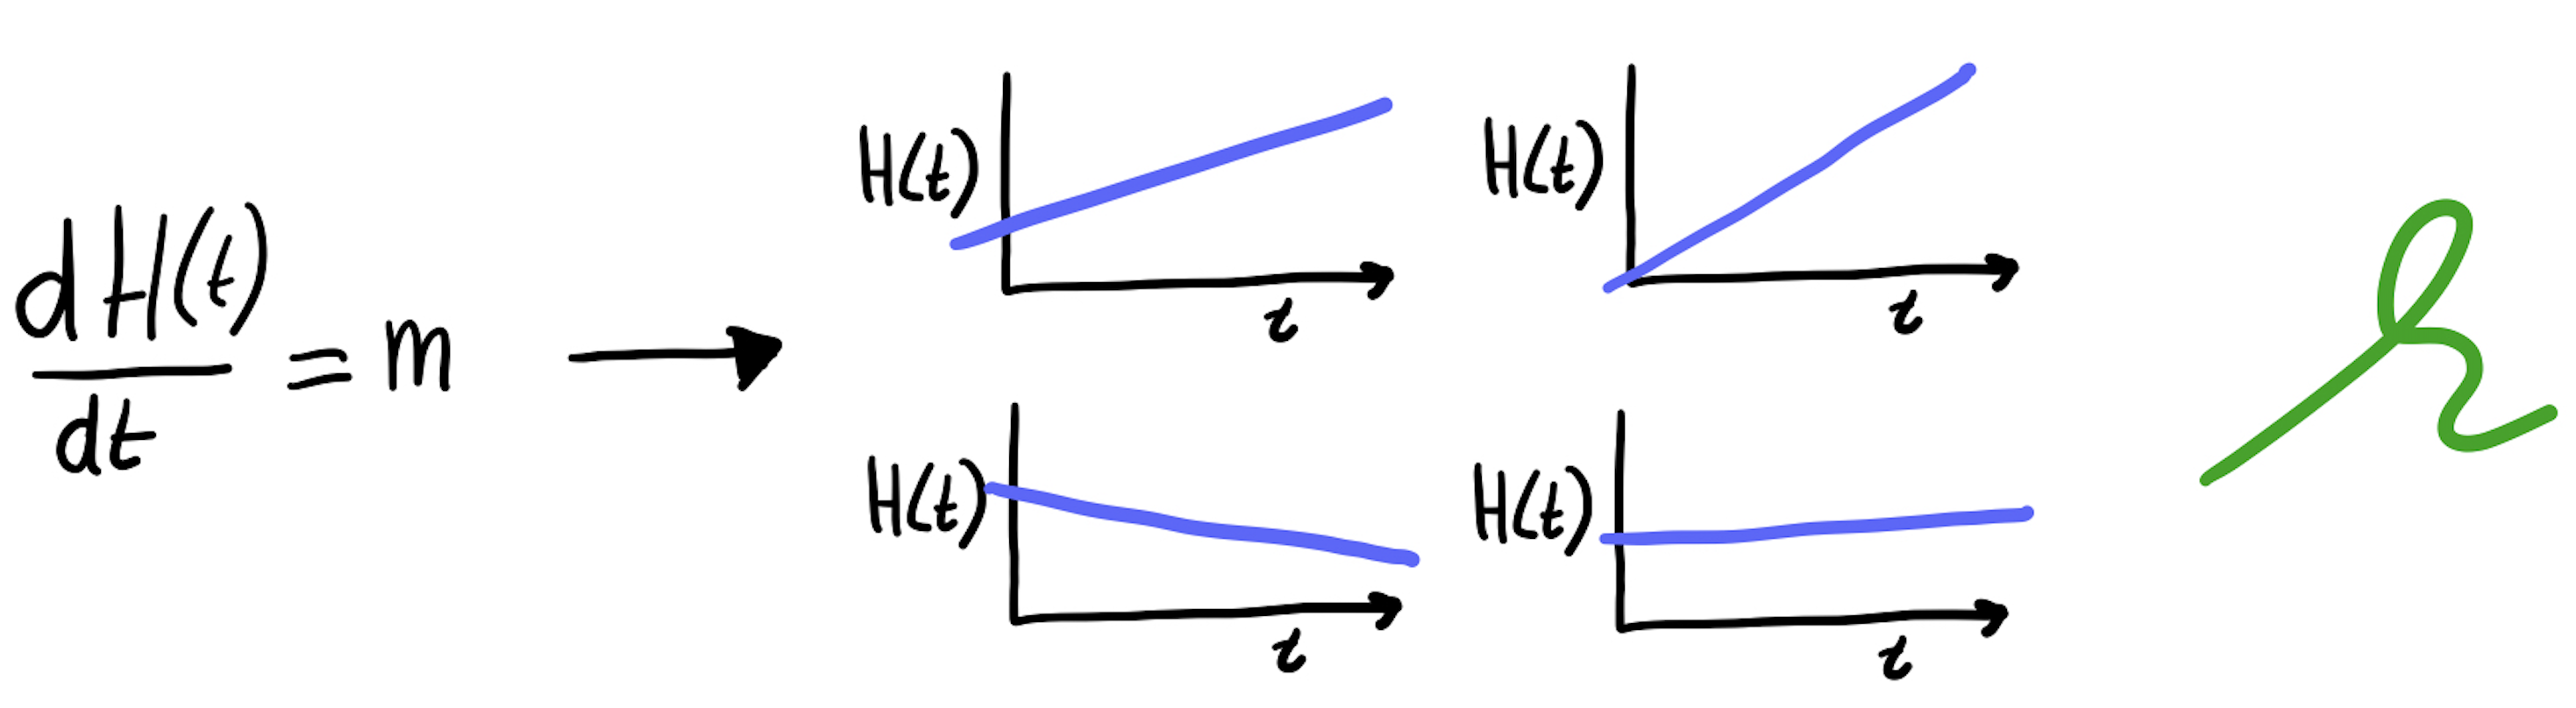
\includegraphics[width=0.95\textwidth,height=\textheight]{Modellering/figuren/solutions_herten_geldig.png}

}

\end{figure}

De oplossing voor onze herten-ODE is dus niet een getal (zoals bij 𝑥 =
6), maar een functie van tijd (``een grafiekje door de tijd''). Er zijn
natuurlijk ook een heleboel grafiekjes die \emph{niet} aansluiten bij
onze ODE:

\begin{figure}

{\centering 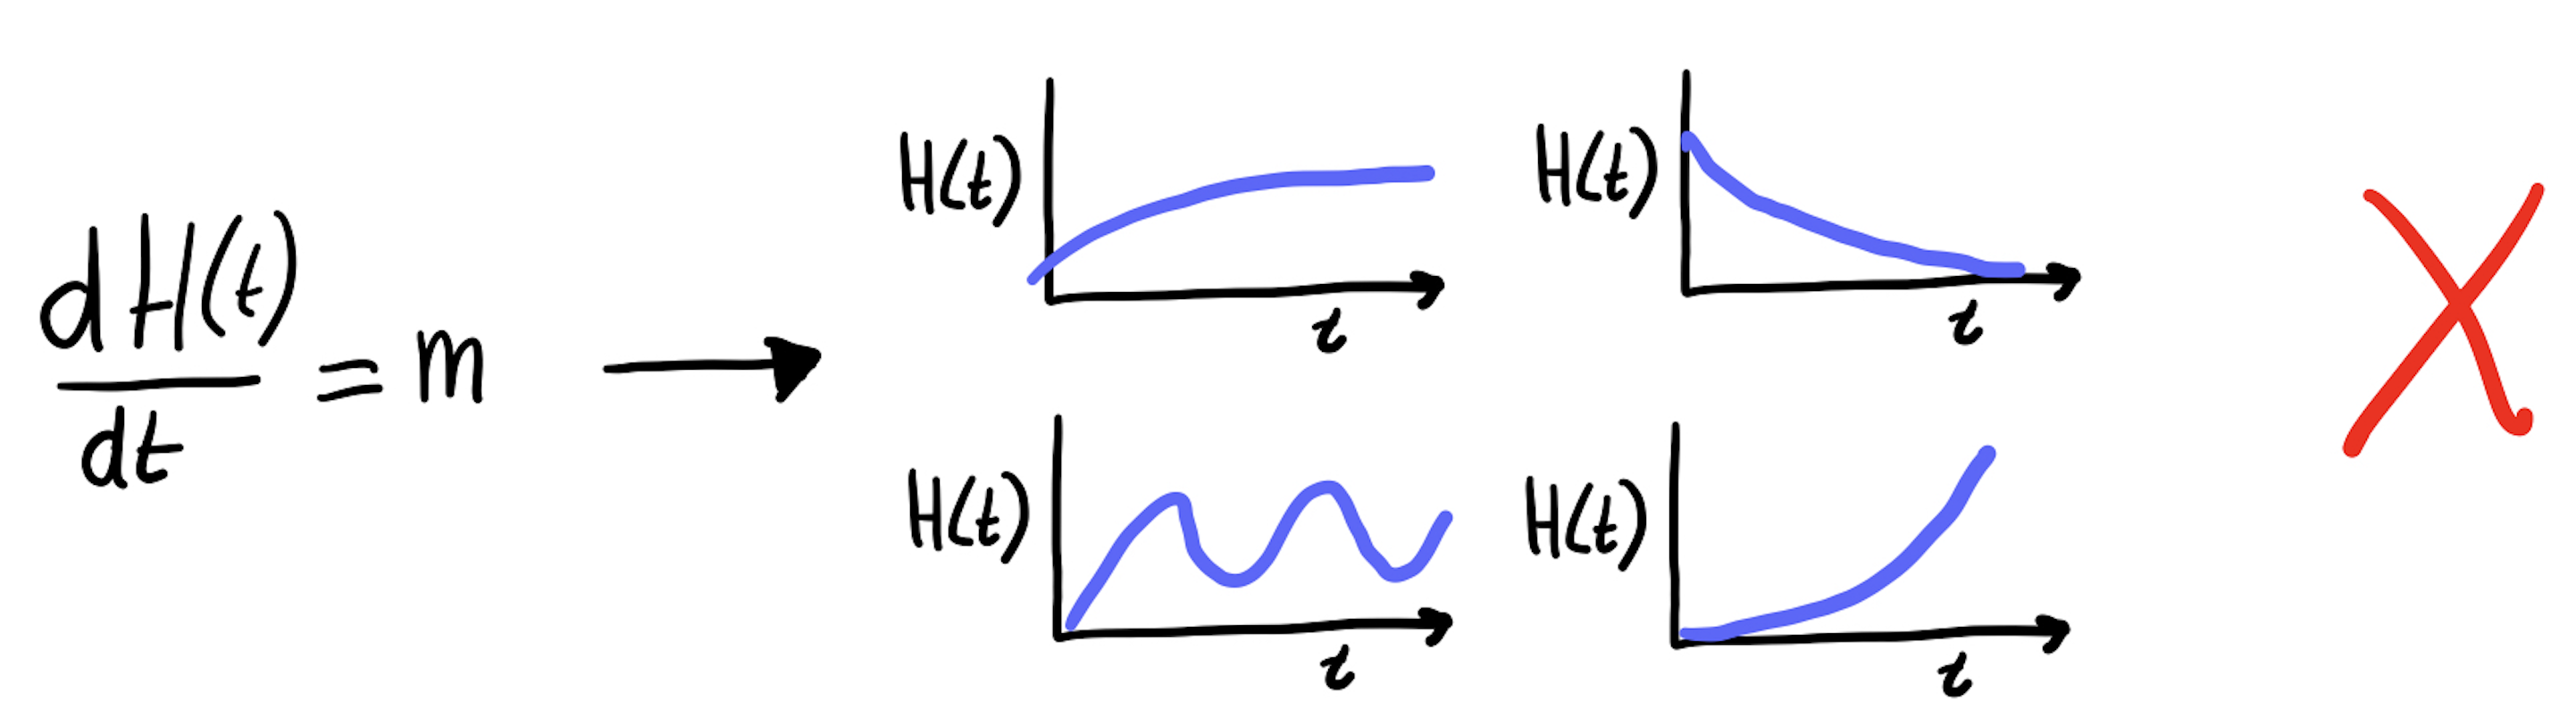
\includegraphics[width=0.95\textwidth,height=\textheight]{Modellering/figuren/solutions_herten_ongeldig.png}

}

\end{figure}

De bovenstaande grafiekjes van \(H(t)\) zijn niet geldig voor onze ODE
van het hertenfeestje, omdat niet op elk punt de helingshoek hetzelfde
is (terwijl de ODE zegt dat deze altijd gelijk is aan \(m\)). Geldige
grafiekjes worden \emph{specifieke oplossingen} genoemd: ze gelden
alleen voor specifieke beginwaarden van \(H\) en een specifieke waarde
van parameter \(m\). Er bestaan ook algemene oplossingen voor ODEs, wat
in dit geval de wiskundige vergelijking is waaraan alle specifieke
oplossingen voldoen. Voor ons hertenfeestje hadden we die al bepaald in
Vergelijking~\ref{eq-ht}. Maar, nogmaals, wat nu als we eerst een ODE
hadden opgesteld? Hoe weten we dan welke oplossing (welke functie /
``grafiekje door de tijd'') daarbij hoort? Deze dynamiek door de tijd is
natuurlijk precies wat we willen weten, zodat we voorspellingen kunnen
doen!

Stel dat de herten ook dood kunnen gaan (toch niet zo'n leuk feestje
dus, maar zo is de natuur). Anders dan met de migratie, hangt de
hoeveelheid sterfte af van de huidige hoeveelheid herten (\(H(t)\)). De
ODE wordt dan dus:

\begin{equation}\protect\hypertarget{eq-ht2}{}{
\mathchoice{\frac{\mathrm{d}H(t)}
{\mathrm{d}t}}{\mathrm{d}H(t)/\mathrm{d}t}
{\mathrm{d}H(t)/\mathrm{d}t}
{\mathrm{d}H(t)/\mathrm{d}t} = m - d \cdot H(t)
}\label{eq-ht2}\end{equation}

\begin{tcolorbox}[enhanced jigsaw, coltitle=black, breakable, bottomtitle=1mm, opacityback=0, colback=white, rightrule=.15mm, title=\textcolor{quarto-callout-important-color}{\faExclamation}\hspace{0.5em}{Let op! \(\mathrm{d}\) en \(d\) zijn niet hetzelfde!}, bottomrule=.15mm, toprule=.15mm, left=2mm, colframe=quarto-callout-important-color-frame, toptitle=1mm, opacitybacktitle=0.6, titlerule=0mm, colbacktitle=quarto-callout-important-color!10!white, leftrule=.75mm, arc=.35mm]

De bovenstaande vergelijking heeft twee verschillende d's. De d aan de
linkerkant van de vergelijking geeft aan dat we het over de afgeleide
hebben. De \(d\) aan de rechterkant van de vergelijking staat voor
\emph{death rate}, en je kunt deze twee dus niet tegen elkaar wegdelen!

\end{tcolorbox}

Welke algemene oplossing (\(H(t)=\dots\)) voldoet nu aan deze
vergelijking? Dat wil zeggen, welke functie \(H(t)\) heeft altijd een
afgeleide die aan deze ODE voldoet? Om dit te bepalen moeten we best
hard gaan rekenen (hiervoor moeten we differentiaalvergelijkingen leren
integreren, wat niet altijd eenvoudig is!). Ik zal jullie gerust
stellen: we gaan dit ook niet doen. Er zijn meerdere redenen waarom dit
niet belangrijk is:

\begin{enumerate}
\def\labelenumi{\arabic{enumi}.}
\tightlist
\item
  Zelfs voor relatief simpele ODEs kan het vinden van de oplossing
  \emph{onmogelijk} zijn (niet slechts moeilijk, maar echt onmogelijk)
\item
  Je kunt met behulp van de computer (in R bijvoorbeeld) eenvoudig
  specifieke oplossingen (``grafiekjes'') doorrekenen
\item
  Je kunt met pen-en-papier veel inzicht uit ODEs krijgen zonder de
  algemene oplossing te bepalen
\end{enumerate}

\begin{exercise}[Differentie- en
differentiaalvergelijkingen]\protect\hypertarget{exr-diffvsdiff}{}\label{exr-diffvsdiff}

Meerkeuzevraag: Welke van de volgende uitspraken beschrijft het
belangrijkste verschil tussen een differentie- en een
differentiaalvergelijking?

\begin{enumerate}
\def\labelenumi{\Alph{enumi})}
\item
  Een differentievergelijking gebruikt altijd kleinere tijdstappen dan
  een differentiaalvergelijking.
\item
  Een differentievergelijking beschrijft veranderingen op discrete
  momenten, terwijl een differentiaalvergelijking veranderingen continu
  beschrijft.
\item
  Een differentiaalvergelijking is eenvoudiger op te lossen dan een
  differentievergelijking.
\item
  Een differentievergelijking geeft alleen benaderingen, terwijl je met
  differentiaalvergelijking altijd exacte oplossingen kan vinden.
\item
  Een differentiaalvergelijking kan alleen gebruikt worden voor complexe
  systemen, terwijl een differentievergelijking alleen voor eenvoudige
  systemen geldt.
\item
  Differentiaalvergelijkingen zijn eenvoudiger met de computer te
  berekenen dan differentievergelijkingen.
\end{enumerate}

\emph{NAAR ANTWOORDENMODEL: B}

\end{exercise}

Later in de cursus gaan we R-scripts gebruiken om specifieke oplossingen
te laten uit te rekenen, maar zoals gezegd kun je met pen-en-papier ook
al veel voor elkaar krijgen. Hiermee oefenenen is belangrijk, want zo
krijgen we een beter gevoel voor ODEs, zodat we eerder doorhebben
wanneer de computer (wellicht door een typfoutje) rare resultaten geeft.
Laten we beginnen met waar al het rekenwerk begint: zorgen dat we appels
met appels vergelijken.

\hypertarget{rekenen-aan-eenheden}{%
\section{Rekenen aan eenheden}\label{rekenen-aan-eenheden}}

Laten we nog even doorgaan met onze onfortuinlijke hertenfeestje met
sterfte:

\begin{align}
\mathchoice{\frac{\mathrm{d}H(t)}
{\mathrm{d}t}}{\mathrm{d}H(t)/\mathrm{d}t}
{\mathrm{d}H(t)/\mathrm{d}t}
{\mathrm{d}H(t)/\mathrm{d}t} = m - d \cdot H(t)
\end{align}

Om het allemaal wat overzichtelijker te houden kunnen we het
vermenigvuldigingsteken (\(\cdot\)) weglaten, en \(H(t)\) opschrijven
als \(H\): \begin{align}
\mathchoice{\frac{\mathrm{d}H}
{\mathrm{d}t}}{\mathrm{d}H/\mathrm{d}t}
{\mathrm{d}H/\mathrm{d}t}
{\mathrm{d}H/\mathrm{d}t} = m - dH
\end{align}

Laten we nogmaals omschrijven wat hier staat. Aan de linkerzijde staat
de snelheid van verandering in de hoeveelheid herten per tijdseenheid.
(in het hertenscenario hadden we het over tijd in uren). De verbale
omschrijving ``per tijdseenheid'' kunnen we wiskundig opschrijven als
\(\frac{1}{t}\) (of \(t^{-1}\), dat is hetzelfde). Hetzelfde geldt
overigens voor ``per hert'', wat zou vertalen naar \(\frac{1}{H}\) of
\(H^{-1}\). Je kunt het woord ``per'' dus vertalen naar ``gedeeld
door''. Dus: ``herten per uur'' kunnen we opschrijven als
\(\frac{H}{t}\).

Aan de linkerkant staat dus iets in termen van herten per uur, dus
\(H \over t\). Aan de rechterzijde staan twee individuele termen,
namelijk \(m\) en \(dH\). Om de differentiaalvergelijking geldig te
houden moeten deze individuele termen dezelfde eenheden hebben, je kan
immers geen appels en peren bij elkaar optellen.

\begin{align}
\underbrace{\mathchoice{\frac{\mathrm{d}H}
{\mathrm{d}t}}{\mathrm{d}H/\mathrm{d}t}
{\mathrm{d}H/\mathrm{d}t}
{\mathrm{d}H/\mathrm{d}t}}_{\text{herten per uur}} = \underbrace{m}_{\text{herten per uur}} - \underbrace{dH}_{\text{herten per uur}}
\end{align} Hieruit kunnen we dus onmiddelijk concluderen dat de
migratieparameter (\(m\)) de eenheden ``herten per uur'' moet hebben.
Als we dus in het veld de migratie gaan meten, weten we wat ons te doen
staat.

Maar wat zijn de eenheden van de parameter \(d\), die de sterfte
bepaald? Hiervoor moeten we deze term gelijk stellen aan \(H/t\), en
oplossen voor \(d\):

\begin{align*}
    dH = H/t \\
    d = 1/t
\end{align*}

Nu weten we dus dat de sterfteparameter de eenheid \(1 \over t\) heeft,
met andere woorden ``per tijdseenheid'' of ``per uur''. Omdat we het
aantal herten hebben weggedeeld, beschrijft deze parameter dus de niet
de \emph{absolute sterfte}, maar de \emph{relatieve sterfte}. Als we
deze parameter in het veld zouden willen meten, zouden we het aantal
gestorven herten per uur moeten meten \emph{gedeelt door het totaal
aantal herten}.

\begin{tcolorbox}[enhanced jigsaw, coltitle=black, breakable, bottomtitle=1mm, opacityback=0, colback=white, rightrule=.15mm, title=\textcolor{quarto-callout-tip-color}{\faLightbulb}\hspace{0.5em}{ODEs doen belangrijke aannames}, bottomrule=.15mm, toprule=.15mm, left=2mm, colframe=quarto-callout-tip-color-frame, toptitle=1mm, opacitybacktitle=0.6, titlerule=0mm, colbacktitle=quarto-callout-tip-color!10!white, leftrule=.75mm, arc=.35mm]

Zoals in de introductie uitgelegd, maken alle modellen aannames. Bij
ODEs maken we ook een paar stevige aannames, namelijk:

\begin{itemize}
\tightlist
\item
  Populatiegroottes zijn continu. \emph{Daarom worden ze meestal als
  dichtheden (en niet aantallen) geïnterpreteerd. }
\item
  Er is geen variatie binnen de populatie (elk hert is gelijk)
\item
  Parameters zijn constant (en meestal ook groter dan \(0\))
\item
  De populatie is goed gemengd (\emph{well-mixed assumption})
\end{itemize}

\end{tcolorbox}

\begin{exercise}[Plastic in de
oceaan]\protect\hypertarget{exr-eenheden-tussen}{}\label{exr-eenheden-tussen}

We omschrijven hoe de hoeveelheid plastic in de oceaan verandert (kilo's
per jaar) met de volgende vergelijking:

\begin{align}
\mathchoice{\frac{\mathrm{d}P}
{\mathrm{d}t}}{\mathrm{d}P/\mathrm{d}t}
{\mathrm{d}P/\mathrm{d}t}
{\mathrm{d}P/\mathrm{d}t} = k - \delta P
\end{align}

\begin{enumerate}
\def\labelenumi{\alph{enumi}.}
\tightlist
\item
  Welke twee processen worden beschreven met de twee individuele termen?
  Beschrijf in je eigen woorden.
\item
  Bepaal de eenheden van de parameter \(k\)
\item
  Bepaal de eenheden van de parameter \(\delta\)?
\item
  Welke parameter (\(k\) of \(\delta\)) denk je dat groter is?
\end{enumerate}

\emph{NAAR ANTWOORDENMODEL: a. dumping en afbraak} \emph{NAAR
ANTWOORDENMODEL: b. kilo's plastic per jaar} \emph{NAAR ANTWOORDENMODEL:
c.~per jaar} \emph{NAAR ANTWOORDENMODEL: d.~k is dumping, dus zal wel
veel groter zijn want plastic breekt niet snel af}

\end{exercise}

\hypertarget{evenwichten}{%
\section{Evenwichten}\label{evenwichten}}

Zoals hierboven uitgelegd is het vaak (relatief) eenvoudig om een ODE
(bijvoorbeeld \(\mathchoice{\frac{\mathrm{d}H}
{\mathrm{d}t}}{\mathrm{d}H/\mathrm{d}t}
{\mathrm{d}H/\mathrm{d}t}
{\mathrm{d}H/\mathrm{d}t} = m - dH\)) op te stellen, maar niet zo
eenvoudig om de algemene oplossing (\(H(t) = ...\)) te vinden. In dit
deel gaan we een ODE-model van de konijnen in Australië bestuderen, en
zul je zien dat we die oplossing ook helemaal niet nodig hebben om
inzichten te vergaren.

Een mogelijk ODE-model voor de exponentiële groei van konijnen ziet er
zo uit:

\begin{equation}
    \frac{\mathrm{d}N(t)}{\mathrm{d}t} = r \cdot N(t)
\end{equation}

Wederom laten we het vermenigvuldigingsteken en de \((t)\) weg, zodat
het iets minder slordig wordt:

\begin{equation}
    \frac{\mathrm{d}N}{\mathrm{d}t} = rN
\end{equation}

De rechterzijde van deze vergelijking lijkt heel erg op de
differentievergelijking uit het vorige hoofdstuk, \emph{maar let op}, de
interpretatie is net anders. Hier staat dat de \emph{groeisnelheid}
gelijk is aan \(rN\), en niet de populatiegrootte in ``de volgende
tijdstap''. Dat betekent dat bij deze ODE elke positieve waarde van
\(r\) (ook \(r=0.1\)) resulteert in groei, terwijl in de
differentievergelijking alleen groei is wanneer \(r>1\). Ondanks deze
verschillen, kunnen we wel een vergelijkbare uitbreiding doen om de
exponentiële groei niet tot in het oneindige door te laten gaan. We
breiden hiervoor de ODE uit met een zogeheten \emph{functionele
response} \(f(N)\):

\begin{equation}
    \frac{\mathrm{d}N}{\mathrm{d}t} = rN \cdot f(N)
\end{equation}

Als de functie \(f(N)\) afneemt bij toenemende hoeveelheid N, dan zal de
groeisnelheid van de populatie dus ook afnemen bij toenemende
hoeveelheid \(N\). We weten bijvoorbeeld dat \(f(N)=1-\frac{N}{100}\)
gelijk wordt aan \(0\) als \(N=100\), dus als we onze ODE
vermenigvuldigen met deze functionele response dan kan de populatie niet
groeien als \(N>=100\). Algemener kunnen we voor dit getal een vrije
parameter voor het draagvermogen (\emph{carrying capacity}) gebruiken
(\(K\)).

\begin{tcolorbox}[enhanced jigsaw, coltitle=black, breakable, bottomtitle=1mm, opacityback=0, colback=white, rightrule=.15mm, title=\textcolor{quarto-callout-warning-color}{\faExclamationTriangle}\hspace{0.5em}{Parameters zijn vaak kleine letters, maar niet altijd}, bottomrule=.15mm, toprule=.15mm, left=2mm, colframe=quarto-callout-warning-color-frame, toptitle=1mm, opacitybacktitle=0.6, titlerule=0mm, colbacktitle=quarto-callout-warning-color!10!white, leftrule=.75mm, arc=.35mm]

Over het algemeen gebruiken we voor variabelen hoofdletters (R, N) en
voor parameters kleine letters (r, d). Dit is echter niet altijd zo,
zoals bij de parameter \(K\), die in de ecologie veel wordt gebruikt
voor de \emph{carrying capacity}.

\end{tcolorbox}

Nu we een functionele response \(f(N) = 1-\frac{N}{K}\) met carrying
capacity hebben gedefinieerd, wordt onze ODE:

\begin{equation}
    \frac{\mathrm{d}N}{\mathrm{d}t} = rN (1-\frac{N}{K})
\end{equation}

Als een populatie groeit volgens de bovenstaande vergelijking, wanneer
is er dan een evenwicht? Wanneer verandert de populatie niet meer? Met
een ODE, is het antwoord daarop vrij eenvoudig: wanneer de snelheid van
verandering (\(\frac{\mathrm{d}K}{\mathrm{d}t}\)) vergelijking gelijk is
aan 0:

\begin{equation}
    0 = rN (1-\frac{N}{K})
\end{equation}

Het gelijk stellen aan \(0\) levert een enorm voordeel op: we raken de
vreemde \(\mathchoice{\frac{\mathrm{d} }
{\mathrm{d}t}}{\mathrm{d} /\mathrm{d}t}
{\mathrm{d} /\mathrm{d}t}
{\mathrm{d} /\mathrm{d}t}\) helemaal kwijt, en hebben daardoor ineens te
maken met een normale algebraïsche vergelijking! Nu kunnen we eenvoudig
uitzoeken bij welke dichtheid (\(N\)) de vergelijking klopt, met andere
woorden we lossen op voor \(N\):

\begin{align*}
    rN (1-\frac{N}{K}) &= 0 \quad \text{ als...}\\
    \color{blue} \bar{N} & \color{blue} = 0  \color{black} \quad \text{ of als...}\\
    (1-N/K) &= 0 \rightarrow \color{blue} \bar{N}=K \\
\end{align*}

Blauw-gedrukt staan de twee oplossingen van onze vergelijking. Soms
(maar lang niet altijd) worden populaties in evenwicht aangegeven met
een streepje boven de variabele, in dit geval \(\bar{N}\). Uit deze
analyse kunnen we concluderen dat de populatie konijnen niet kan groeien
wanneer \(N=0\) (als er geen konijnen zijn) of als \(N=K\) (als de
populatie gelijk is aan de carrying capacity). Het eerste evenwicht
(\(N=0\)) wordt vaak een ``triviaal'' evenwicht genoemd: als populaties
niet bestaan kunnen ze ook niet groeien. Het tweede evenwicht (\(N=K\))
is echter biologisch inzichtelijker: de populatie groeit totdat de
carrying capacity is bereikt.

We kunnen dezelfde strategie gebruiken om te controleren of pure
exponentiële groei een evenwicht heeft:

\begin{align*}
    \mathchoice{\frac{\mathrm{d}N}
{\mathrm{d}t}}{\mathrm{d}N/\mathrm{d}t}
{\mathrm{d}N/\mathrm{d}t}
{\mathrm{d}N/\mathrm{d}t} &= rN = 0 \quad \text{ als...}\\
    N &= 0 &
\end{align*}

Exponentiële groei heeft dus alleen een zogezegd triviaal evenwicht.

\begin{tcolorbox}[enhanced jigsaw, coltitle=black, breakable, bottomtitle=1mm, opacityback=0, colback=white, rightrule=.15mm, title=\textcolor{quarto-callout-caution-color}{\faFire}\hspace{0.5em}{Parameters zijn niet nul}, bottomrule=.15mm, toprule=.15mm, left=2mm, colframe=quarto-callout-caution-color-frame, toptitle=1mm, opacitybacktitle=0.6, titlerule=0mm, colbacktitle=quarto-callout-caution-color!10!white, leftrule=.75mm, arc=.35mm]

ODEs kunnen ook gelijk zijn aan nul als parameters 0 zijn. Echter zijn
dit vaak onzinnige inzichten (een model van exponentiële groei zonder
groei is onzinnig). Daarom bekijken we vooral bij welke
\emph{populatiegroottes} (of dichtheden) er evenwichten zijn.

\end{tcolorbox}

Laten we ook kijken of ons hertenfeestje evenwichten heeft:

\begin{align*}
    \mathchoice{\frac{\mathrm{d}H}
{\mathrm{d}t}}{\mathrm{d}H/\mathrm{d}t}
{\mathrm{d}H/\mathrm{d}t}
{\mathrm{d}H/\mathrm{d}t} &= m = 0 \quad \text{ als...}\\
\end{align*}

Zoals uitgelegd in (\textbf{nte-parsnul?}) nemen we aan dat parameters
niet \(0\) zijn (een model van hertenmigratie zonder migratie is geen
model), en zijn we dus vooral geintresseerd in welke dichtheden \(H\)
evenwicht geven. Voor deze vergelijking bestaat er dus geen evenwicht,
want welke waarde voor \(H\) je ook invult, de populatie blijft met een
constante snelheid \(m\) veranderen. Voor het onfortuinlijke feestje met
sterfte, ligt dat net anders:

\begin{align*}
    \mathchoice{\frac{\mathrm{d}H}
{\mathrm{d}t}}{\mathrm{d}H/\mathrm{d}t}
{\mathrm{d}H/\mathrm{d}t}
{\mathrm{d}H/\mathrm{d}t} &= m - dH = 0 \quad \text{ als...}\\
    dH &= m & \\
    H &= \frac{m}{d} &
\end{align*}

De populatie herten op het feestje zal dus uiteindelijk uitkomen op een
evenwicht (\(H\)) van \(\frac{m}{d}\) herten. Op dit moment gaan er
kennelijk evenveel herten dood als er naar het bos toe migreren.

Dus: als we willen weten waar het evenwicht van een een ODE
\(\mathchoice{\frac{\mathrm{d}X}
{\mathrm{d}t}}{\mathrm{d}X/\mathrm{d}t}
{\mathrm{d}X/\mathrm{d}t}
{\mathrm{d}X/\mathrm{d}t}\) ligt, stellen we de ODE gelijk aan \(0\) en
lossen we de vergelijking op voor \(X\). Als de vergelijking geen \(X\)
bevat (of als \(X\) wegvalt), dan is er geen evenwichtssituatie.

\hypertarget{opgaven-1}{%
\section{Opgaven}\label{opgaven-1}}

\begin{exercise}[Plastic in de oceaan
(evenwicht)]\protect\hypertarget{exr-eenheden-tussen2}{}\label{exr-eenheden-tussen2}

Bekijk nogmaals de volgende vergelijking voor hoe snel de hoeveelheid
plastic in de oceaan verandert:

\begin{align}
\mathchoice{\frac{\mathrm{d}P}
{\mathrm{d}t}}{\mathrm{d}P/\mathrm{d}t}
{\mathrm{d}P/\mathrm{d}t}
{\mathrm{d}P/\mathrm{d}t} = k - \delta P
\end{align}

\begin{enumerate}
\def\labelenumi{\alph{enumi}.}
\tightlist
\item
  Bepaal bij elke hoeveelheid plastic er sprake is van een
  evenwichtssituatie (\emph{steady state})
\item
  Is er een triviaal (\(P=0\)) evenwicht?
\item
  Stel we vissen morgen (op een magische manier) alle plastic uit de
  oceaan. Schets met pen-en-paper wat er daarna zal gebeuren.
\end{enumerate}

\emph{NAAR ANTWOORDENMODEL: a. k/delta} \emph{NAAR ANTWOORDENMODEL: b.
nee} \emph{NAAR ANTWOORDENMODEL: c.~zelfs als er geen plastic is, er
wordt constant gedumpt, dus het gaat natuurlijk gewoon weer toenemen
tenzij we ons gedrag aanpassen. plastic `groeit' niet exponentieel, dus
het zal lineair beginnen en naar een evenwicht van k/delta teruggaan
(voorbeeld-schets invoegen!!)}

\end{exercise}

\begin{exercise}[Rode
bloedcellen]\protect\hypertarget{exr-rodebloedcellen}{}\label{exr-rodebloedcellen}

\begin{figure}

{\centering 
\includegraphics[width=0.5\textwidth,height=\textheight]{Modellering/figuren/rode_bloedcellen.png}

}

\caption{Rode bloedcellen, of rode CUTEcellen? Gegenereerd met
ChatGPT4-o}

\end{figure}

Rode bloedcellen worden in het beenmerg geproduceerd met een snelheid
\(p\) cellen per dag. Elke rode bloedcel kan sterven met een kans \(d\)
per dag.

\begin{enumerate}
\def\labelenumi{\alph{enumi}.}
\tightlist
\item
  Dit process levert dezelfde ODEs op als het bovengenoemde model voor
  plastic in de oceaan. Schrijf de vergelijking
  (\(\frac{\mathrm{d}B}{dt} = \dots\)) op. \emph{dB/dt = p - dB}
\item
  Wat zijn de eenheden van de parameters \(p\) en \(d\)? \emph{p =
  cellen per dag, d = per dag. Zelfde idee als herten.}
\item
  Reken uit hoeveel bloedcellen er in het evenwicht zijn. \emph{dB/dt =
  0 geeft p - dB = 0, p = dB, B = p/d}
\item
  Stel je doneert een halve liter bloed. Maak met pen en papier een
  schets van de hoeveelheid bloedcellen over de tijd vlak na de donatie.
  \emph{zelfde idee als met plastic hierboven, hoewel niet ALLES
  weggehaald wordt}
\item
  Stel nu dat je juist bloed ontvangt. Maak nog een schets van de
  hoeveelheid bloedcellen over de tijd. \emph{correcte schets voor
  antwoordenmodel nodig!!}
\item
  Welke van deze twee parameters denk je dat de snelheid van het herstel
  bepaalt? \emph{Intuitief zou je misschien p denken (we zien later dat
  dit niet zo is)}
\item
  Je hebt geleerd dat het vinden van algemene oplossingen van ODEs heel
  moeilijk kan zijn (met andere woorden, de exacte functie \(B(t)\) die
  aan onze bloed-cellen ODE voldoet is lastig). Echter kunnen we de
  specifieke oplossing van een ODE wel doorrekenen als we de
  begin-hoeveelheid en de parameters van het model invullen. Als we deze
  waarden weten, kunnen we met R numeriek een specifieke oplossing
  doorrekenen. \textbf{Analyseer het onderstaande script regel voor
  regel, en lees de comments en zorg dat je begrijpt wat er gebeurt}.
\end{enumerate}

\begin{Shaded}
\begin{Highlighting}[]
\CommentTok{\# Stap 1: stel parameters in}
\NormalTok{p }\OtherTok{\textless{}{-}} \FloatTok{2e11}    
\NormalTok{d }\OtherTok{\textless{}{-}} \DecValTok{1}\SpecialCharTok{/}\DecValTok{120}   

\CommentTok{\# Stap 2: stel het beginaantal B in}
\NormalTok{B }\OtherTok{\textless{}{-}}\NormalTok{ p}\SpecialCharTok{/}\NormalTok{d}

\CommentTok{\# Stap 3: maak functie die B, p, en d gebruikt om de verandering uit te rekenen}
\NormalTok{verandering }\OtherTok{\textless{}{-}} \ControlFlowTok{function}\NormalTok{ (B, p, d)\{}
\NormalTok{  delta }\OtherTok{\textless{}{-}}\NormalTok{ p}\SpecialCharTok{{-}}\NormalTok{ d}\SpecialCharTok{*}\NormalTok{B}
  \FunctionTok{return}\NormalTok{(delta)}
\NormalTok{\}}

\CommentTok{\# Stap 4: een test of de functie werkt}
\FunctionTok{verandering}\NormalTok{(}\AttributeTok{B=}\NormalTok{p}\SpecialCharTok{/}\NormalTok{d, }\AttributeTok{p=}\NormalTok{p, }\AttributeTok{d=}\NormalTok{d) }

\CommentTok{\# Stap 5: maak een lege lijst met begin{-}aantal erin}
\NormalTok{B }\OtherTok{\textless{}{-}} \FunctionTok{c}\NormalTok{(}\FloatTok{0.9}\SpecialCharTok{*}\NormalTok{p}\SpecialCharTok{/}\NormalTok{d)}

\CommentTok{\# Stap 6: reken 500 keer de volgende hoeveelheid B uit}
\ControlFlowTok{for}\NormalTok{ (t }\ControlFlowTok{in} \DecValTok{1}\SpecialCharTok{:}\DecValTok{500}\NormalTok{) \{}
\NormalTok{  B[t}\SpecialCharTok{+}\DecValTok{1}\NormalTok{] }\OtherTok{\textless{}{-}}\NormalTok{ B[t] }\SpecialCharTok{+} \FunctionTok{verandering}\NormalTok{(}\AttributeTok{B=}\NormalTok{B[t], }\AttributeTok{p=}\NormalTok{p, }\AttributeTok{d=}\NormalTok{d)}
\NormalTok{\}}

\CommentTok{\# Stap 7: plot de tijdserie}
\FunctionTok{plot}\NormalTok{(B, }\AttributeTok{xlab=}\StringTok{"Tijd in dagen"}\NormalTok{, }\AttributeTok{ylab=}\StringTok{"Aantal rode bloedcellen"}\NormalTok{, }\AttributeTok{type=}\StringTok{"l"}\NormalTok{, }\AttributeTok{col=}\StringTok{"red"}\NormalTok{, }\AttributeTok{lwd=}\DecValTok{2}\NormalTok{)}
\end{Highlighting}
\end{Shaded}

\begin{enumerate}
\def\labelenumi{\alph{enumi}.}
\setcounter{enumi}{7}
\tightlist
\item
  In regel 15 rekent het script de hoeveelheid verandering in \(B\) uit.
  Waarom geeft de functie \(0\) terug? \emph{je begint met
  evenwichtshoeveelheid B, dus er is geen verandering!}
\item
  De code in de for-loop produceert een specifieke oplossing, dat wil
  zeggen het rekent één van de mogelijke tijd-series uit voor \(B(t)\).
  Dit gebeurt op een zeer grove manier door in stappen de integraal (de
  opsomming van kleine veranderingen) door te rekenen. Om dit netjes te
  doen, gebruik je normaal gesproken integrators die automatisch zorgen
  dat de tijdstap niet te groot is\footnote{Hiervoor gaan we later in de
    cursus een R-script genaamd Grind.R inladen}. Leg uit waarom dat
  belangrijk kan zijn (hint: denk aan het vorige hoofdstuk). \emph{grote
  tijdstappen kunnen soms problemen geven, dat hebben ze voor de
  logistische groei al gezien.}
\item
  Schat met behulp van de grafiek in hoe lang het duurt om de helft van
  het bloedverlies te herstellen. \emph{ongeveer 100 dagen, daarom moet
  je tussen donaties 3-4 maanden wachten}
\item
  Stel dat je slechts een beetje bloed verliest (0.1\%). Hoe lang duurt
  het om hiervan de helft te herstellen? \emph{Zelfde snelheid! De helft
  is nu wel veel minder, maar het herstel gaat even snel}.
\item
  Wat bepaalt denk je hoe snel je van bloedverlies herstelt (\(p\),
  \(d\), of beide)? \emph{ze zullen vast p denken}
\item
  Gebruik het script om te bepalen welke parameter (\(p\) of \(d\)) de
  snelheid van herstel bepaalt. Komt dit overeen met je eerdere
  inschatting? \emph{d bepaald het, niet p.~Veel van hen zullen dit
  verkeerd inschatten (denk ik) }
\end{enumerate}

\end{exercise}

::: \{\#exr-diffvsdiffinR\} \#\# Een differentie- en
\textbf{differentiaal}vergelijking doorrekenen met R

We hebben eerder een R-script bekeken die een tijdserie produceert van
een differentievergelijking voor logistische konijnengroei, waar de
populatiegrootte in de variabele ``konijnen'' stond. Om de leesbaarheid
te vergroten worden vaak kortere namen gebruikt voor parameters en
variabelen (meestal enkele letters), bijvoorbeeld \(N\) voor aantal
konijnen, en \(r\) voor de intrinsieke groeisnelheid. Het R-script zie
er dan bijvoorbeeld zo uit:

\begin{Shaded}
\begin{Highlighting}[]
\CommentTok{\# SIMPEL SCRIPT VOOR DIFFERENTIEVERGELIJKING}
\CommentTok{\# Stap 1, definieer beginaantal konijnen en parameters}
\NormalTok{N }\OtherTok{\textless{}{-}} \DecValTok{24}    \CommentTok{\# aantal konijnen}
\NormalTok{r }\OtherTok{\textless{}{-}} \DecValTok{2}     \CommentTok{\# intrinsieke groeisnelheid}
\NormalTok{K }\OtherTok{\textless{}{-}} \DecValTok{10}\SpecialCharTok{\^{}}\DecValTok{9}  \CommentTok{\# schaalt de dichtheidsafhankelijkheid}

\CommentTok{\# Stap 2: bereken het aantal konijnen in [t+1] 40 keer}
\ControlFlowTok{for}\NormalTok{ (t }\ControlFlowTok{in} \DecValTok{1}\SpecialCharTok{:}\DecValTok{40}\NormalTok{)\{}
\NormalTok{  N[t}\SpecialCharTok{+}\DecValTok{1}\NormalTok{] }\OtherTok{\textless{}{-}}\NormalTok{ r}\SpecialCharTok{*}\NormalTok{N[t]}\SpecialCharTok{*}\NormalTok{(}\DecValTok{1}\SpecialCharTok{{-}}\NormalTok{(N[t]}\SpecialCharTok{/}\NormalTok{K))}
\NormalTok{\}}

\CommentTok{\# Stap 3: bekijk resultaten}
\NormalTok{N[}\DecValTok{20}\NormalTok{] }\CommentTok{\# Aantal na 20 halve jaren}
\FunctionTok{plot}\NormalTok{(N,}\AttributeTok{type=}\StringTok{"o"}\NormalTok{,}\AttributeTok{xlab=}\StringTok{"Tijd (jaren)"}\NormalTok{, }\AttributeTok{ylab=}\StringTok{"Aantal konijnen"}\NormalTok{)}
\end{Highlighting}
\end{Shaded}

We kunnen een vergelijkbaar script gebruiken om de ODE
(differen\emph{tiaal}vergelijking) van konijnengroei door te rekenen.
Let op: ODEs hebben in werkelijkheid geen ``tijdstappen'\,' (tijd is een
continue variabele), maar een computer werkt eigenlijk altijd in
stappen. We moeten dus in ieder geval zorgen dat we kleine stapjes
nemen. Neem de onderstaande code over en zorg dat je de regels zo goed
mogelijk begrijpt.

\begin{Shaded}
\begin{Highlighting}[]
\CommentTok{\# SIMPEL SCRIPT VOOR DIFFERENTIAALVERGELIJKING}
\CommentTok{\# Stap 1, definieer beginaantal konijnen en parameters}
\NormalTok{N }\OtherTok{\textless{}{-}} \DecValTok{24} 
\NormalTok{r }\OtherTok{\textless{}{-}} \DecValTok{2}
\NormalTok{K }\OtherTok{\textless{}{-}} \DecValTok{10}\SpecialCharTok{\^{}}\DecValTok{9}

\CommentTok{\# Stap 2, definieer tijdstappen en maak een dataframe aan}
\NormalTok{delta\_t }\OtherTok{\textless{}{-}} \FloatTok{0.0001} \CommentTok{\# grootte van de tijdstap}
\NormalTok{tijdstapjes }\OtherTok{\textless{}{-}} \FunctionTok{seq}\NormalTok{(}\DecValTok{0}\NormalTok{,}\DecValTok{20}\NormalTok{,}\AttributeTok{by=}\NormalTok{delta\_t)}
\NormalTok{tijdserie }\OtherTok{\textless{}{-}} \FunctionTok{data.frame}\NormalTok{(}\AttributeTok{t=}\NormalTok{tijdstapjes,}\AttributeTok{konijnen=}\NormalTok{N)}

\CommentTok{\# Stap 3: Reken in kleine stapjes de volgende N uit}
\ControlFlowTok{for}\NormalTok{ (t }\ControlFlowTok{in} \DecValTok{1}\SpecialCharTok{:}\FunctionTok{length}\NormalTok{(tijdstapjes)}\SpecialCharTok{{-}}\DecValTok{1}\NormalTok{)\{}
\NormalTok{  groeiN }\OtherTok{\textless{}{-}}\NormalTok{ delta\_t }\SpecialCharTok{*}\NormalTok{ r}\SpecialCharTok{*}\NormalTok{N}\SpecialCharTok{*}\NormalTok{(}\DecValTok{1}\SpecialCharTok{{-}}\NormalTok{N}\SpecialCharTok{/}\NormalTok{K)  }
\NormalTok{  N }\OtherTok{\textless{}{-}}\NormalTok{ N }\SpecialCharTok{+}\NormalTok{ groeiN }
\NormalTok{  tijdserie[t}\SpecialCharTok{+}\DecValTok{1}\NormalTok{,}\StringTok{"konijnen"}\NormalTok{] }\OtherTok{\textless{}{-}}\NormalTok{ N}
\NormalTok{\}}

\CommentTok{\# Stap 3: bekijk resultaten}
\NormalTok{tijdserie[}\DecValTok{20}\NormalTok{,] }\CommentTok{\# Aantal na 0.19 jaar}
\FunctionTok{plot}\NormalTok{(tijdserie}\SpecialCharTok{$}\NormalTok{t, tijdserie}\SpecialCharTok{$}\NormalTok{konijnen, }\AttributeTok{type=}\StringTok{"l"}\NormalTok{,}\AttributeTok{xlab=}\StringTok{"Tijd (jaren)"}\NormalTok{, }\AttributeTok{ylab=}\StringTok{"Aantal konijnen"}\NormalTok{)}
\end{Highlighting}
\end{Shaded}

Het bovenstaande script is iets anders geschreven dan het eerste script.
Simpele scripts kunnen vaak op heel veel manieren geschreven worden. Zo
genereert de bovenstaande code niet een tijdserie-vector (zoals het
vorige voorbeeld), maar een tijdserie-dataframe. Het voordeel hiervan is
dat we ook een tweede kolom kunnen bijhouden: de hoeveelheid tijd die is
verstreken.

\begin{enumerate}
\def\labelenumi{\alph{enumi}.}
\tightlist
\item
  Bestudeer het eerste R-script (voor de
  \textbf{differentie}vergelijking). Voer het script uit voor veel
  verschillende waarden van \(r\). Wat gebeurt er met \(r<1\)? Wat
  gebeurt er met \(r>3.7\)?
\item
  Bestudeer ook het R-script voor de \textbf{differentiaal}vergelijking.
  Wat gebeurt er met \(r<1\)? \textbackslash{} Wat gebeurt er met
  \(r>3.7\)? Welke waarde van \(r\) geeft afname? Welke Bij welke waarde
  van \(r\) krijg je chaotische fluctuaties?
\item
  Maak de tijdstap voor de differentiaalvergelijking heel klein (bijv
  \(delta_t = 0.0001\)), en voer het hele script uit. Wat valt je op?
  (hint: R-studio heeft rechtsboven in de console een grote rode
  STOP-knop)
\end{enumerate}

\emph{NAAR ANTWOORDEN: a. Vanaf r \textgreater{} 3 krijg je fluctuaties,
r\textgreater3.7 chaos. b. r\textless1 geeft ook groei! belangrijk
verschil. r\textgreater3.7 geeft geen chaos! Je moet r behoorlijk hoog
opschroeven om dat toch te vinden, want de tijdstapjes zijn klein (250
werkt) c.~dat het langzaam wordt. ODEs zijn dus precieser, maar dat
wordt ook steeds moeilijker voor je computers. Dit is waarom je meestal
betere tools gebruikt om ODEs te integreren, zoals GrindR ;D}

\hypertarget{terminologie-2}{%
\section{Terminologie}\label{terminologie-2}}

\begin{longtable}[]{@{}
  >{\raggedright\arraybackslash}p{(\columnwidth - 4\tabcolsep) * \real{0.2466}}
  >{\raggedright\arraybackslash}p{(\columnwidth - 4\tabcolsep) * \real{0.2740}}
  >{\raggedright\arraybackslash}p{(\columnwidth - 4\tabcolsep) * \real{0.4795}}@{}}
\toprule\noalign{}
\begin{minipage}[b]{\linewidth}\raggedright
Nederlands
\end{minipage} & \begin{minipage}[b]{\linewidth}\raggedright
Engels
\end{minipage} & \begin{minipage}[b]{\linewidth}\raggedright
Beschrijving
\end{minipage} \\
\midrule\noalign{}
\endhead
\bottomrule\noalign{}
\endlastfoot
Differentiaalvergelijking / ODE & Differential equation / ODE & Een
wiskundige vergelijking die omschrijft hoe snel een variabele
(bijvoorbeeld een populatiegrootte) verandert. \\
Specifieke oplossing van een ODE & Specific solution of an ODE & Eén van
de vele mogelijke oplossingen van een ODE, bijvoorbeeld door specifieke
parameters / begin-hoeveelheden in te vullen \\
Algemene oplossing & General solution & De wiskundige vergelijking waar
alle specifieke oplossingen aan voldoen. Meestal moeilijk te
verkrijgen. \\
Functionele response & Functional response & Een (meestal eenvoudige)
wiskundige functie die de relatie omschrijft tussen de snelheid waarmee
een proces verloopt, en de grootte van een variabele \\
Evenwicht & Equilibrium / steady state & We spreken van een
evenwichtssitautie als alle processen elkaar opheffen, zodat de
variabelen van het systeem niet meer veranderen. \\
Triviaal evenwicht & Trivial equilibrium & Een evenwichts-situatie die
biologisch gezien niet interessant is, bijvoorbeeld een evenwicht bij
\(0\) konijnen. \\
\end{longtable}

\hypertarget{sec-dichtheid}{%
\chapter{Dichtheidseffecten}\label{sec-dichtheid}}

In het vorige onderdeel heb je geleerd dat een populatie in evenwicht is
als hun snelheid van verandering gelijk is aan 0. Zodoende bereikte de
populatie die eerst exponentiëel groeide, een evenwicht bij een bepaald
draagvermogen: de \textbf{carrying capacity}. In dit onderdeel gaan we
explicieter zijn over \emph{hoe} een carrying capacity nou eigenlijk
bepaald wordt, door naar veranderingen in geboorte- en sterftesnelheden
te kijken.

\hypertarget{leerdoelen-3}{%
\section{Leerdoelen}\label{leerdoelen-3}}

Na dit hoofdstuk, moet je het volgende kunnen:

\begin{itemize}
\tightlist
\item
  Uitleggen wat een functionele response is, en veelgebruikte (zoals
  dichtheidsafhankelijke geboorte, \emph{density dependent birth})
  kunnen herkennen
\item
  Een faseportret kunnen lezen, en corresponderende oplossing schetsen
\item
  Uitleggen waarom het afschieten van dieren positieve effecten kan
  hebben op dierwelzijn.
\end{itemize}

\begin{figure}

{\centering 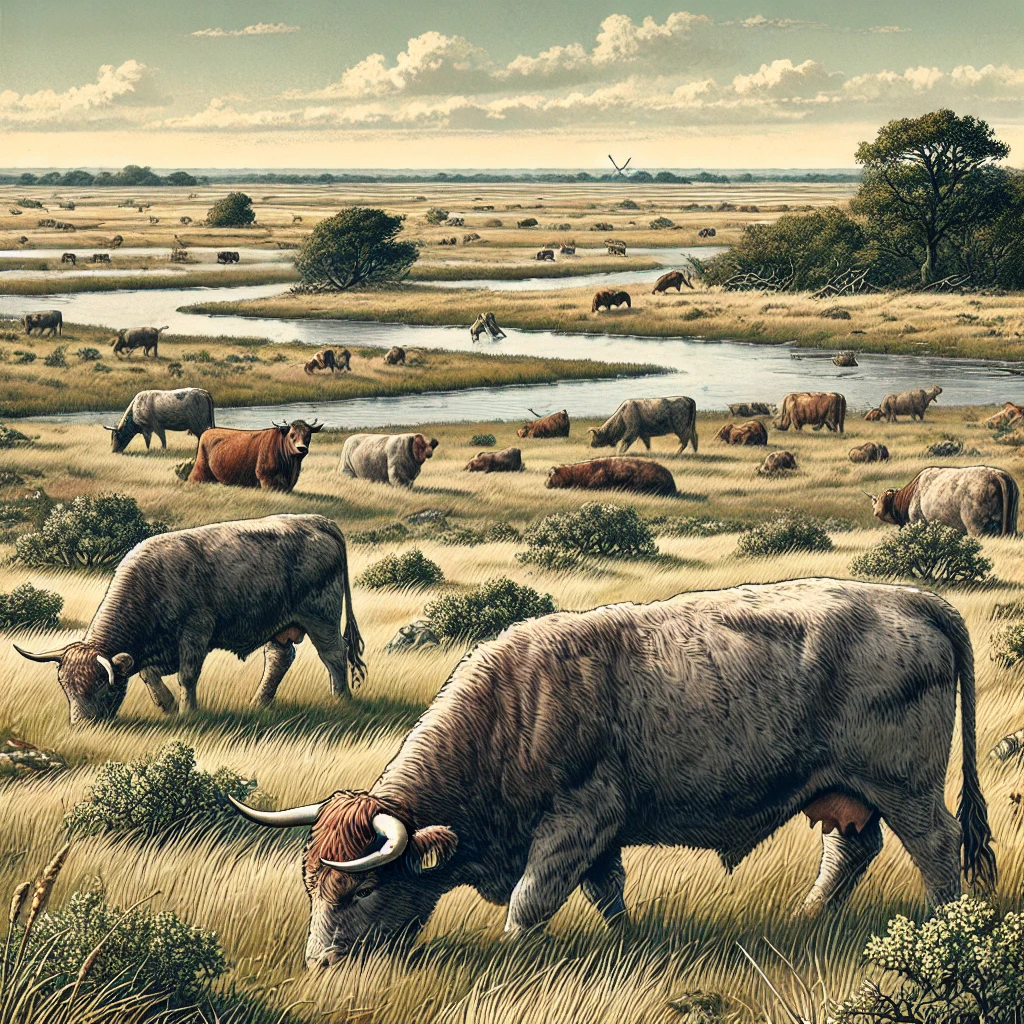
\includegraphics[width=0.8\textwidth,height=\textheight]{Modellering/figuren/heck_ai.png}

}

\caption{Afbeelding gegenereerd met ChatGPT4-o}

\end{figure}

\hypertarget{geboorte-en-sterfte}{%
\section{Geboorte en sterfte}\label{geboorte-en-sterfte}}

In het vorige onderdeel hebben we dichtheidsafhankelijkheid ingebouwd
zodat de populatie langzamer gaat groeien bij grote dichtheden:

\[
\frac{\mathrm{d}N}{\mathrm{d}t} = rN(1-\frac{N}{K})
\]

De parameter \(r\) in deze vergelijking staat bekend als de
\textbf{intrinsieke groeisnelheid} (\emph{intrinsic growth rate}) van de
populatie. Als \(r\) positief is, is er groei (ook als \(r=0.1\)!). Als
\(r\) negatief is de groei negatief. Maar biologisch gezien is
``negatieve groei'' natuurlijk een beetje vreemd. Bedoelen we niet
eigenlijk dat de hoeveelheid sterfte (hierna: \emph{death}) hoger is dan
geboorte (hierna: \emph{birth})? Een gebrek aan voedsel kan bijvoorbeeld
een verhoogde death rate opleveren, terwijl birth rate gelijk blijft.
Het zou ook zo kunnen dat individuen met minder voedsel minder
reproduceren (dus een verlaagde birth rate krijgen). Om deze verbale
begrippen in onze ODE te verwerken, moeten we afstappen van de parameter
\(r\), en deze uitsplitsen in birth (\(b\)) en death (\(d\)).
Bijvoorbeeld, neem ons model van exponentiële groei:

\[
    \frac{\mathrm{d}N}{\mathrm{d}t} = rN 
\]

Nogmaals: in dit model is er exponentiele groei wanneer \(r>0\), en
exponentiele afname wanneer \(r<0\). Als we r vervangen door het
verschil in birth (\(b\)) en death (\(d\)), dan krijgen we:

\begin{equation}\protect\hypertarget{eq-rbd}{}{
    \frac{\mathrm{d}N}{\mathrm{d}t} = (\color{blue}b\color{black}-\color{red}d\color{black})N
}\label{eq-rbd}\end{equation}

\begin{tcolorbox}[enhanced jigsaw, coltitle=black, breakable, bottomtitle=1mm, opacityback=0, colback=white, rightrule=.15mm, title=\textcolor{quarto-callout-caution-color}{\faFire}\hspace{0.5em}{Let op! Vergelijking~\ref{eq-rbd} geeft ook gewoon exponentiele groei
(of afname)!}, bottomrule=.15mm, toprule=.15mm, left=2mm, colframe=quarto-callout-caution-color-frame, toptitle=1mm, opacitybacktitle=0.6, titlerule=0mm, colbacktitle=quarto-callout-caution-color!10!white, leftrule=.75mm, arc=.35mm]

Hoewel we twee nieuwe parameters hebben geintroduceerd, is er weinig
veranderd aan ons model. Net als dat \(r>0\) en \(r<0\) respectievelijk
leidde tot groei en afname, is er bij \(b>d\) en \(b<d\) ook sprake van
exponentiële groei of afname:

\begin{figure}[H]

{\centering 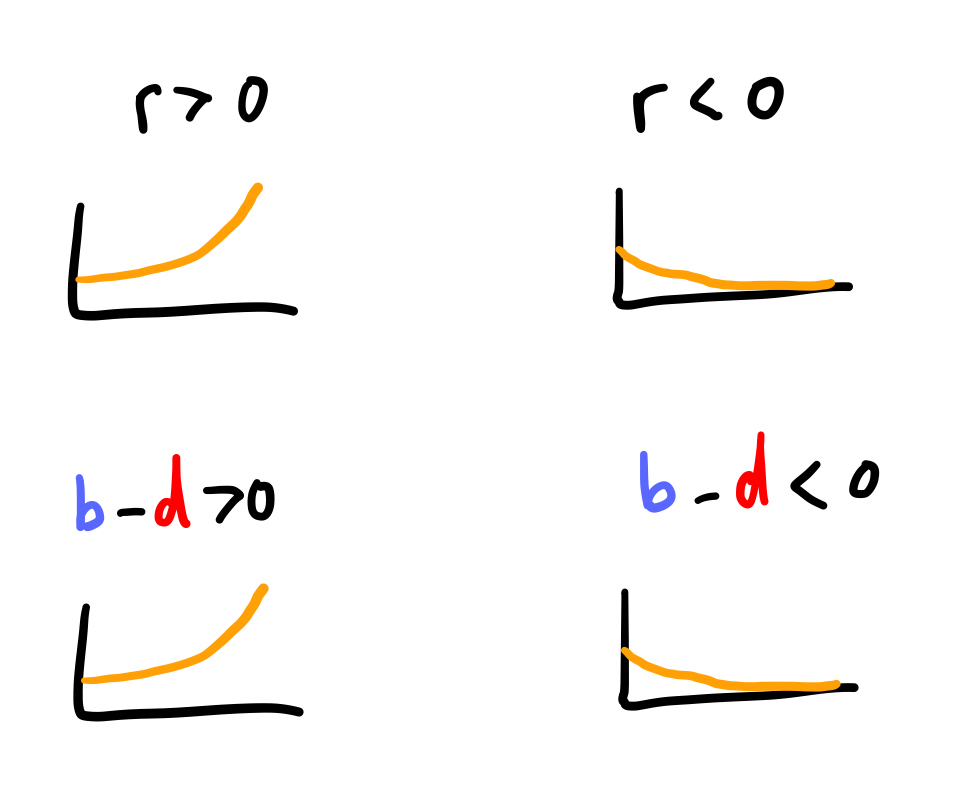
\includegraphics[width=0.5\textwidth,height=\textheight]{Modellering/figuren/exponential_with_bd_vs_r.png}

}

\end{figure}

\end{tcolorbox}

\hypertarget{dichtheidsafhankelijke-geboorte}{%
\section{Dichtheidsafhankelijke
geboorte}\label{dichtheidsafhankelijke-geboorte}}

Hoewel onze nieuwe vergelijking voor groei nog niet heel anders is,
kunnen we met deze aanpassing wel na gaan denken over \emph{birth} en
\emph{death} processen. Stel je voor dat we experimenteel hebben bepaald
dat een soort dichtheidsafhankelijke geboorte heeft (\emph{density
dependent birth}), zie bijvoorbeeld Figuur~\ref{fig-ddbpears}.

\begin{figure}

{\centering 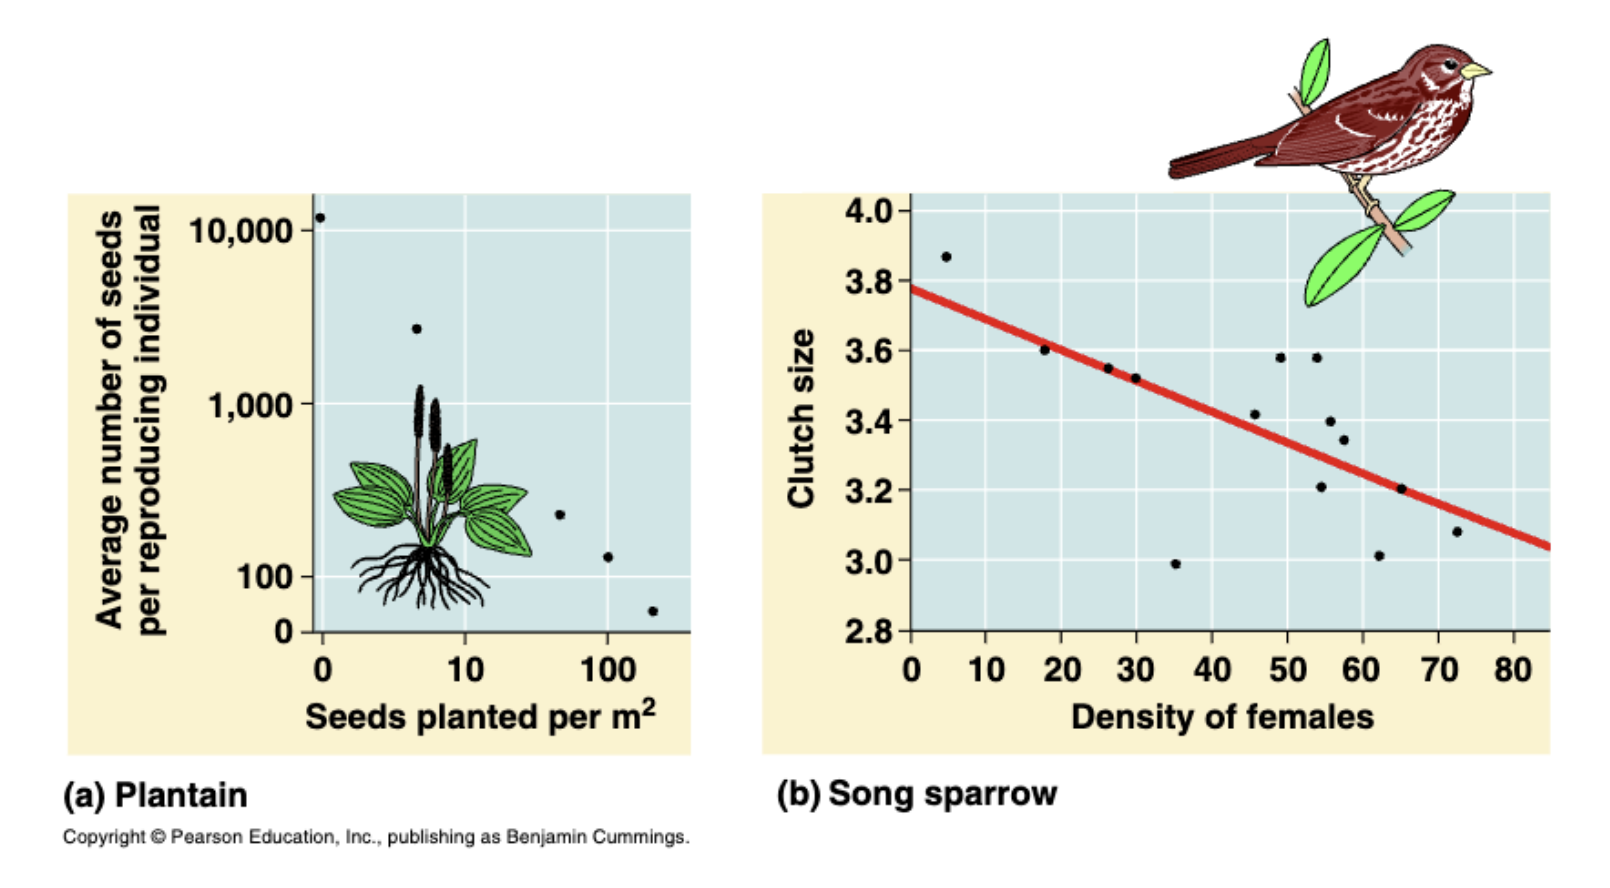
\includegraphics{Modellering/figuren/ddb_pears.png}

}

\caption{\label{fig-ddbpears}Reproductiesucces neemt vaak af met
dichtheid (© 2014 Pearson Education Inc.)}

\end{figure}

Waar we deze afname eerder in het gehele groei-process hadden verwerkt
door aan te nemen dat \(r\) kleiner werd, gaan we nu een nieuw model
bekijken waar alleen de birth verandert bij grotere dichtheden. Hiervoor
is het handig om eerst de birth en death termen op te splitsen:

\begin{align}
    \frac{\mathrm{d}N}{\mathrm{d}t} &= (\color{blue}b\color{black}-\color{red}d\color{black})N\\
    \frac{\mathrm{d}N}{\mathrm{d}t} &= \color{blue}b\color{black}N - \color{red}d\color{black}N
\end{align}

Nu kunnen we ervoor kiezen om voor de geboorteterm met een
\textbf{functionele response} aan te passen:

\begin{align}
    \color{blue}b\color{black} & \rightarrow \color{blue}b\color{black} \cdot f(N)
\end{align}

Bijvoorbeeld dezelfde functionele response die we eerder hebben
gebruikt:

\begin{align}
    \color{blue}b\color{black} & \rightarrow \color{blue}b\color{black}(1-\frac{N}{K}) 
\end{align}

Dat wil zeggen, de constante parameter \(b\) wordt vervangen door een
term die afneemt met \(N\). De parameter \(b\) staat nu niet meer voor
de birth rate, maar voor de \emph{maximale birth rate} die alleen
bereikt wordt bij kleine populatiegroottes. Als we dit in de gehele ODE
invullen, krijgen we nu:

\begin{align}
    \frac{\mathrm{d}N}{\mathrm{d}t} &= \color{blue}b\color{black}(1-\frac{N}{K})N - \color{red}d\color{black}N
\end{align}

\begin{exercise}[Andere functionele
responses]\protect\hypertarget{exr-functioneleresponses}{}\label{exr-functioneleresponses}

Hierboven gebruiken we de functionele response \(f(N)=1-\frac{N}{K}\) om
geboorte af te laten nemen. Leg uit waarom de volgende functionele
responses wel/niet een vergelijkbaar effect zullen hebben:

\begin{enumerate}
\def\labelenumi{\alph{enumi}.}
\tightlist
\item
  \(f(N)=\frac{N}{K} + 1\)
\item
  \(f(N)= 1 - cN\)
\item
  \(f(N)= 1 - cN^2\)
\end{enumerate}

\emph{ANTWOORD: a. Niet, want geboorte neemt toe met N, b. Wel, gegeven
dat c = 1/K is het dezelfde. c.~Niet, want deze neemt kwadratisch af met
dichtheid. Maar het neemt iig wel af!}

\end{exercise}

\hypertarget{het-faseportret}{%
\section{Het faseportret}\label{het-faseportret}}

Zoals je in het vorige hoofdstuk geleerd hebt, kunnen we ODEs eenvoudig
analyseren door ons af te vragen: wanneer is er geen groei meer? Wanneer
is \(\mathchoice{\frac{\mathrm{d}N}
{\mathrm{d}t}}{\mathrm{d}N/\mathrm{d}t}
{\mathrm{d}N/\mathrm{d}t}
{\mathrm{d}N/\mathrm{d}t}\) gelijk aan \(0\)? Deze relatief eenvoudige
berekening word weergegeven in de linkerzijde van
Figuur~\ref{fig-faseportret}. De rechterzijde geeft visueel weer wat
deze berekening nou eigenlijk heeft bepaald, door de groeisnelheid (dus:
de ODE) als functie van de dichtheid van de populatie te schetsen. Als
we de ODE uitvermenigvuldigen zien we een negatieve tweede-orde term
(\(-bN^2/k\)) en twee eerste-orde termen (\(bN\) en \(dN\) zijn niet
gekwadrateerd). Dit vormt een bergparabool\footnote{Als je functies
  schetsen lastig vindt, kijk dan nog even naar hoofdstuk
  (\textbf{section-schetsen?}). Je kan het ook altijd even controleren
  met de website \textless Desmos.com\textgreater{}}, een functie die op
twee punten gelijk is aan \(0\). Op deze punten is de populatie in
evenwicht: deze kan niet groeien of krimpen.

\begin{figure}

{\centering 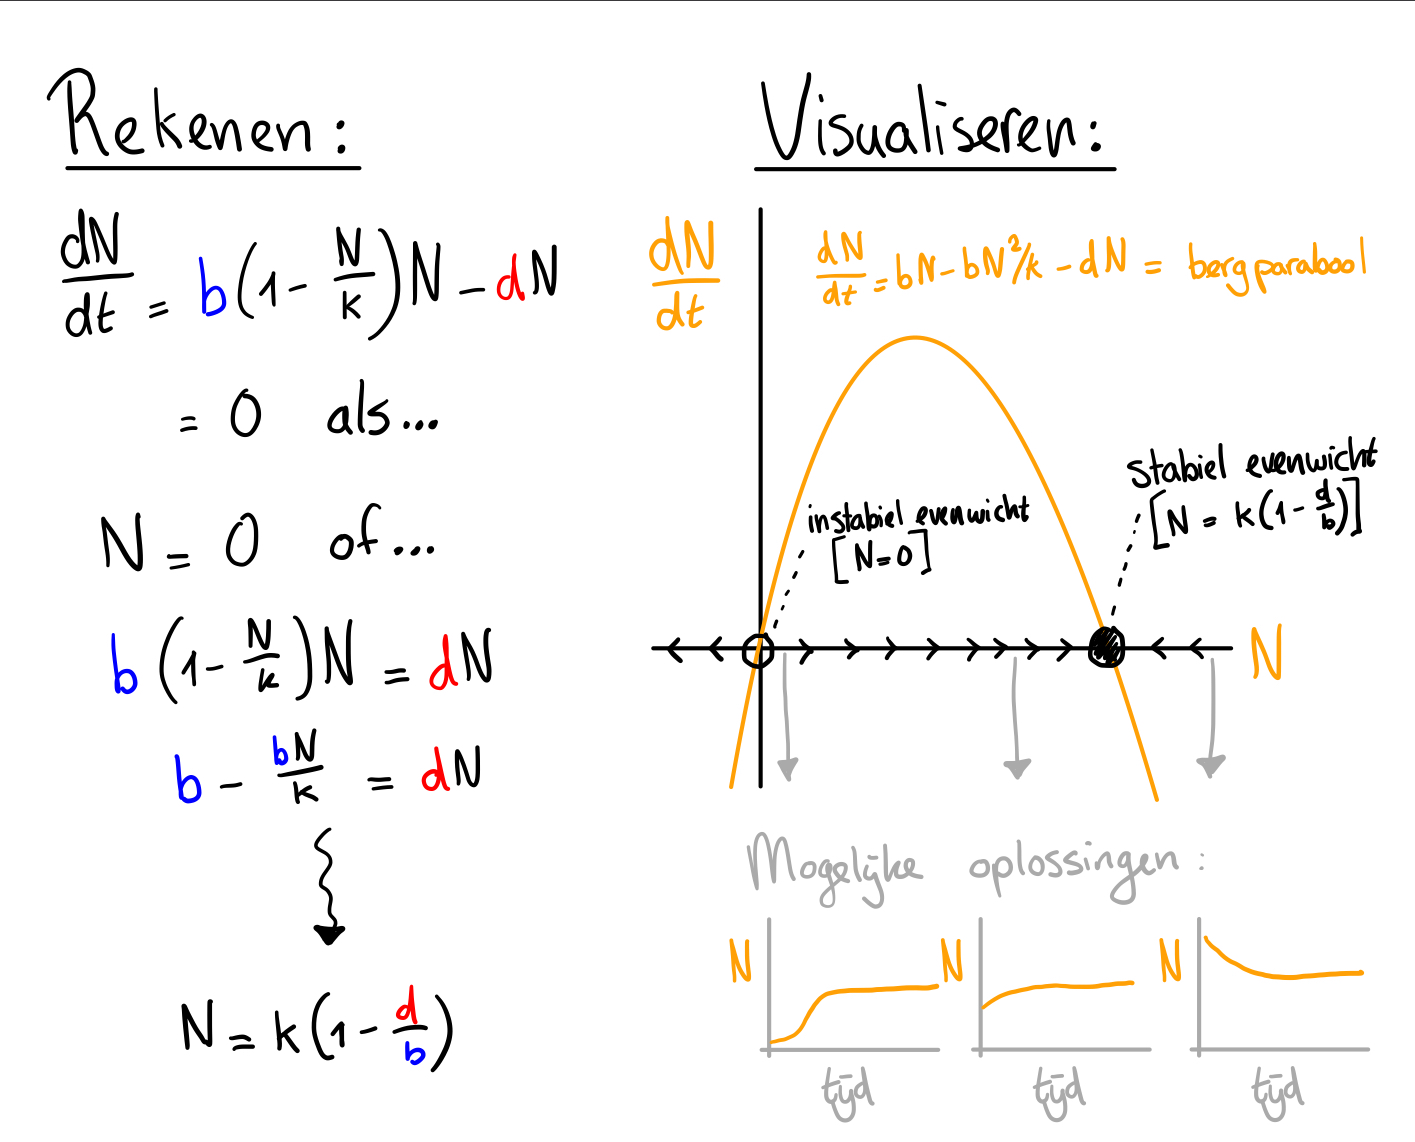
\includegraphics[width=0.8\textwidth,height=\textheight]{Modellering/figuren/faseportret_logistische_groei.png}

}

\caption{\label{fig-faseportret}Rekenen aan evenwichten, of deze
visualiseren in een faseportret}

\end{figure}

Er is nog iets wat je heel snel aan een faseportret af kan lezen. We
weten dat er groei is als \(\mathchoice{\frac{\mathrm{d}N}
{\mathrm{d}t}}{\mathrm{d}N/\mathrm{d}t}
{\mathrm{d}N/\mathrm{d}t}
{\mathrm{d}N/\mathrm{d}t}\) groter is dan \(0\), dat de populatie
afneemt als \(\mathchoice{\frac{\mathrm{d}N}
{\mathrm{d}t}}{\mathrm{d}N/\mathrm{d}t}
{\mathrm{d}N/\mathrm{d}t}
{\mathrm{d}N/\mathrm{d}t}\) kleiner is dan \(0\) (en zoals gezegd: dat
er een evenwicht is als \(\mathchoice{\frac{\mathrm{d}N}
{\mathrm{d}t}}{\mathrm{d}N/\mathrm{d}t}
{\mathrm{d}N/\mathrm{d}t}
{\mathrm{d}N/\mathrm{d}t}\) gelijk is aan \(0\)). In het figuur staan
deze punten aangegeven op de x-as. Pijltjes naar rechts geven aan dat er
groei is (pijltje wijst naar ``meer N''), pijltjes naar links geven aan
dat er afname is, en cirkels geven aan dat er een evenwicht is. Als de
pijltjes naar dit evenwicht toewijzen, dan zal het systeem daar op ten
duur naartoe gaan. Zo'n \textbf{stabiel evenwicht} wordt ook wel een
\textbf{attractor} genoemd, en wordt vaak aangegeven met een ingevulde
cirkel. Het evenwicht bij \(N=0\) heeft alleen pijltjes die ervan
wegwijzen, en is dus een \textbf{instabiel evenwicht} (en is geen
attractor). Deze worden vaak aangegeven met een open cirkel. Dankzij
deze visualisatie is het relatief eenvoudig om te bedenken hoe het
systeem zich over de tijd zal ontwikkelen. Voor specifieke
begin-waarden, kunnen we dus \emph{specifieke oplossingen} schetsen!

\hypertarget{dichtheidsafhankelijke-sterfte}{%
\section{Dichtheidsafhankelijke
sterfte}\label{dichtheidsafhankelijke-sterfte}}

Op een vergelijkbare manier als hierboven, zouden we ook een populatie
kunnen modelleren die dichtheidsafhankelijke sterfte (\emph{density
dependent death}) ondergaat:

\begin{align}
    \color{red}d\color{black} & \rightarrow \color{red}d\color{black}(1+\frac{N}{K}) \\
    \frac{\mathrm{d}N}{\mathrm{d}t} &= \color{blue}b\color{black} - \color{red}d\color{black}(1+\frac{N}{K})
\end{align}

Let op dat we hier de sterfte laten \emph{toenemen} met de dichtheid (er
staat een \(+\) in plaats van een \(-\)).

\begin{exercise}[Rekenen aan dichtheidsafhankelijke
sterfte]\protect\hypertarget{exr-dddportrait}{}\label{exr-dddportrait}

Hierboven hebben we een ODE opgesteld voor dichtheidsafhankelijke
sterfte, namelijk: \[
\frac{\mathrm{d}N}{\mathrm{d}t} = \color{blue}b\color{black} - \color{red}d\color{black}(1+\frac{N}{K})
\] Bekijk nog eens Figuur~\ref{fig-faseportret}.

\begin{enumerate}
\def\labelenumi{\alph{enumi}.}
\tightlist
\item
  Bereken waar de evenwichten liggen met de dichtheidsafhankelijke
  sterfte
\item
  Schets het faseportret en geef aan waar eventuele evenwichten liggen.
\end{enumerate}

\end{exercise}

\hypertarget{andere-dichtheidseffecten}{%
\section{Andere dichtheidseffecten}\label{andere-dichtheidseffecten}}

In de natuur zal het vaak zo zijn dat zowel geboorte als sterfte door de
populatiegrootte worden beinvloed, dus moeten we ook beide in ons model
opnemen. Dan krijgen we:

\begin{align}
    \frac{\mathrm{d}N}{\mathrm{d}t} &= \color{blue}b\color{black}(1-\frac{N}{K_b})N - \color{red}d\color{black}(1+\frac{N}{K_d})N\\
\end{align}

Hier schaalt \(K_b\) de dichtheidsafhankelijke geboorte, en \(K_d\) de
dichtheidsafhankelijke sterfte. In het werkcollege zullen jullie zien
dat dit simpele model inzicht kan geven in belangrijke
beleidsbeslissingen met betrekking tot dierenwelzijn.

Er zijn vele andere mogelijke dichtheidseffecten mogelijk (teveel om te
benoemen). Als we het over ecosystemen hebben, zullen er ook effecten
zijn die afhangen van de dichtheid van een \emph{andere} soort. We
kunnen ons bijvoorbeeld voorstellen dat de konijnen (\(N\)) door vossen
(\(V\)) worden opgegeten. Hoe meer konijnen en vossen, hoe
waarschijnlijker het wordt dat konijnen worden weggegeten: dus dit is
ook een dichtheidseffect:

\begin{align}
    \frac{\mathrm{d}N}{\mathrm{d}t} &= \color{blue}b\color{black}(1-\frac{N}{K_b})N - \color{red}d\color{black}(1+\frac{N}{K_d})N - cNV\\
\end{align}

Deze vergelijking begint er aardig ingewikkeld uit te zien, maar doordat
we het stapje voor stapje hebben opgebouwd, zie je wellicht goed in wat
elke term betekent. In de laatste (nieuwe term), staat \(c\) voor de
predatiesnelheid is en \(V\) de hoeveelheid vossen. Maar vossen zouden
zelf dan toch ook van populatiegrootte moeten veranderen? In hoofdstuk
Hoofdstuk~\ref{sec-meerdere} ga je zien hoe we ons model kunnen
uitbreiden om zowel konijnen (prooi) als vossen (predator) te kunnen
beschrijven.

\hypertarget{opgaven-2}{%
\section{Opgaven}\label{opgaven-2}}

\begin{exercise}[Bacteriën in het
bloed]\protect\hypertarget{exr-bacterienbloed}{}\label{exr-bacterienbloed}

\begin{figure}

{\centering 
\includegraphics[width=0.8\textwidth,height=\textheight]{Modellering/figuren/tandenpoetsen.png}

}

\caption{Afbeelding gegenereerd met ChatGPT4-o}

\end{figure}

Elke keer dat je je tanden poetst, komt er een kleine hoeveelheid
bacteriën in je bloed. Omdat bloed een erg voedselrijke omgeving is voor
bacteriën, zouden ze hier onmiddelijk exponentieel kunnen groeien.
Gelukkig hebben we neutrofielen in ons bloed die de bacteriën snel
opruimen. Hier zouden we een simpel ODE model voor opstellen:

\[\mathchoice{\frac{\mathrm{d}B}
{\mathrm{d}t}}{\mathrm{d}B/\mathrm{d}t}
{\mathrm{d}B/\mathrm{d}t}
{\mathrm{d}B/\mathrm{d}t}=rB-kNB \]

Hier is B de hoeveelheid bacterien in je bloed is, N de hoeveelheid
neutrofielen in je bloed, \(r\) de groeisnelheid van de bacteriën (per
uur), en k de snelheid waarmee neutrofielen bacteriën opruimen.

\begin{enumerate}
\def\labelenumi{\alph{enumi}.}
\tightlist
\item
  Leg uit waar je denkt dat iedere term in de ODE voor staat, en welke
  eenheden deze termen hebben. \emph{eerste term is exp groei van
  bacterien, tweede term is killing door neutrofielen. De eenheden zijn
  allemaal in bacterien per uur}
\item
  Wat zijn de eenheden voor \(r\) en \(k\)? \emph{r is per uur, k is per
  neutrofiel per uur. Als ze dit niet snappen, moet het ze het stukje
  over het hertenfeest nog een keer lezen: uitrekenen door de termen
  gelijk te zetten aan B/t en op te lossen voor de parameter.}
\item
  Als er geen bacteriën zijn (\(B=0\)) is er geen groei. Dit wordt een
  triviaal (irrelevant) evenwicht genoemd, omdat we voor dit inzicht het
  hele model niet hadden hoeven maken. Neem aan dat er een constante
  hoeveelheid neutrofielen in je bloed zijn (\(N\) is constant). Is er
  een niet-triviaal evenwicht van bacteriën? \emph{nee, de enige andere
  optie is exponentiele groei, wanneer er niet genoeg neutrofielen zijn
  om is de eerste term groter dan de tweede term}
\item
  Chemotherapie kan een groot effect hebben op het aantal neutrofielen
  in het bloed, waardoor de tweede term steeds kleiner wordt. Schets de
  termen \(rB\) en \(kNB\) als een functie van \(N\) (dat wil zeggen,
  met \(N\) op de x-as, en deze termen op de y-as. \emph{horizontale
  lijn en lineair toenemende lijn.}
\item
  Bepaal hoeveel neutrofielen je minimaal nodig hebt om de groei van de
  bacteriën te stoppen. \emph{dit is het snijpunt wat ze net geschetst
  hebben. N\textgreater=r/k}
\item
  De \(kNB\) term heet een \emph{mass-action} term omdat de snelheid
  direct proportioneel is aan de dichtheden van \(N\) en \(B\). Wat
  moeten we doen als we willen weten hoeveel bacteriën er ``per
  neutrofiel'' opgeruimd worden? \emph{deze term telen door N, want ze
  hebben geleerd dat `per' altijd vertaald in `gedeeld door'}
\item
  Hoeveel bacteriën worden er per neutrofiel opgeruimd als er 0
  bacteriën zijn? En als er 1000 bacteriën zijn? En als er oneindig
  bacteriën zijn? Is dit een redelijke aanname? \emph{0, 1000, oneindig.
  Nee, 1 neutrofiel kan niet oneindig veel bacterien aan (kost
  bijvoorbeeld tijd)}
\item
  Bekijk devolgende uitbreiding van ons model
  \[\mathchoice{\frac{\mathrm{d}B}
  {\mathrm{d}t}}{\mathrm{d}B/\mathrm{d}t}
  {\mathrm{d}B/\mathrm{d}t}
  {\mathrm{d}B/\mathrm{d}t}=rB-\frac{kNB}{h+B}  \] De vernieuwde
  (tweede) term ziet er misschien wat ingewikkeld uit. Om te begrijpen
  wat er gebeurt is het wederom handig om even na tegaan wat er gebeurt
  met 0 of heel veel bacterien. Als er 0 bacterien zijn is deze term 0,
  omdat boven de breuk een \(B\) staat. Als \(B\) heel groot is, hoe
  belangrijk is \(h\) dan nog in deze vergelijking? \emph{niet heel
  belangrijk meer, uiteindelijk `verwaarloosbaar'}
\item
  Als er dus heel veel bacterien zijn, hoeveel bacterien kunnen er dan
  per neutrofiel opgeruimd worden in dit nieuwe model? \emph{Gaat naar
  maximaal k per neutrofiel, h+B dus h valt weg, kan je B wegdelen, daat
  er kN. Dus per neutrofiel k.}
\item
  Bepaal opnieuw hoeveel neutrofielen je minimaal nodig hebt om de groei
  van bacteriën te stoppen. \emph{nu moet deze tweede term groter zijn
  dan de eerste: kNB/(B+h) \textgreater= rB geeft N \textgreater=
  r(B+h)/k}
\end{enumerate}

\end{exercise}

\begin{exercise}[Heckrunderen]\protect\hypertarget{exr-heck}{}\label{exr-heck}

Heckrunderen zijn in de Oostvaardersplassen geintroduceerd als
``semi-natuurlijke'' grazers. Ze voorkomen dat het hele gebied begroeid
raakt met bomen en struikgewas, wat belangrijk is voor het broeden van
vogels in dit gebied. In 1983 zijn een kleine populatie heckrunderen
vrijgelaten, en de populatie is na 20 jaar gestabiliseerd op 300-400
runderen.

\begin{figure}

{\centering 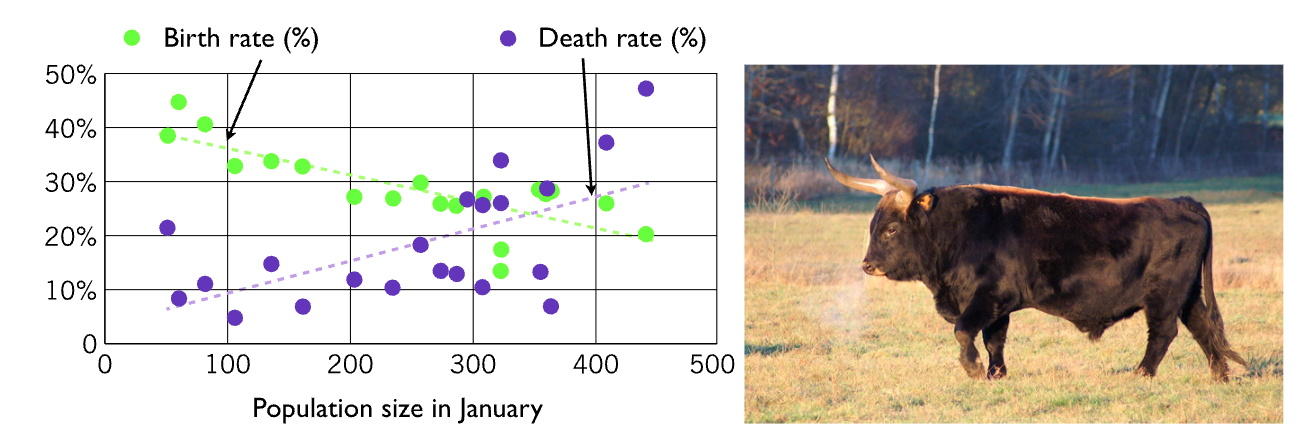
\includegraphics{Modellering/figuren/heck.png}

}

\caption{Heckrunderen op de Oostvaardersplassen}

\end{figure}

Omdat er veel dieren van de honger doodgaan, zijn er veel debatten
geweest over dierenwelzijn. Een mogelijke oplossen is het afschieten van
dieren. Dit zou hun populatiegrootte kunnen verkleinen en daardoor de
overgebleven individuen een prettiger leven geven.

\begin{enumerate}
\def\labelenumi{\alph{enumi}.}
\tightlist
\item
  Bekijk bovenstaande metingen van de geboorte- en sterfte van
  heckrunderen. Hoeveel heckrunderen zou je op basis van deze data
  verwachten in evenwicht? \emph{350 ofzo, waar b en d kruisen, dus dat
  klopt met de aantallen}
\end{enumerate}

De data laat zien dat zowel geboorte als sterfte dichtheidsafhankelijk
zijn. In het hoofdstuk hebben we hier al een model voor besproken: \[
      \frac{\mathrm{d}N}{\mathrm{d}t} = \color{blue}b\color{black}(1-\frac{N}{K_b})N - \color{red}d\color{black}(1+\frac{N}{K_d})N
  \]

Uit het figuur kunnen we zien dat geboorte hoogstens 0.4 per jaar is, en
dat deze bij 400 gehalveerd is.

\begin{enumerate}
\def\labelenumi{\alph{enumi}.}
\setcounter{enumi}{1}
\item
  Wat zijn dan de parameters \(b\) en \(K_b\)? \emph{b is simpelweg 0.4.
  Kb bepaal je door de vergelijking 0.4(1-400/Kb)=1/2 x0.4 op te lossen
  (die laatste kunnen mensen vaak intuitief wel, maar snappen niet wat
  de formele manier is om dat te doen :'{]})}
\item
  In de figuur zien we ook dat sterfte minimaal 0.03 is, en dat deze
  0.33 is bij een populatiegrootte van 500. Wat zijn dan de parameters
  \(d\) en \(K_d\)? \emph{d is weer simpelweg 0.03, Kd vind je door
  0.03(1+500/Kd)=0.33 op te lossen.}
\item
  Vul de parameterwaarden die hebt gevonden in, en bepaal bij welke
  populatiegrootte er een evenwicht is. \emph{parameters invullen en
  dN/dt=0 oplossen (uit mijn hoofd: 330, SAs please check even :)) }
\item
  Hoeveel dieren gaan er in dit evenwicht per jaar dood? \emph{uit mijn
  hoofd iets van 78, zoiets iig}
\item
  Om het afschieten van runderen in dit model te betrekken, kunnen we
  een extra term aan de ODE toevoegen: \[
    \frac{\mathrm{d}N}{\mathrm{d}t} = \color{blue}b\color{black}(1-\frac{N}{K_b})N - \color{red}d\color{black}(1+\frac{N}{K_b})N - kN
    \] Waarbij \(k\) de fractie runderen is die we afschieten. Bekijk
  hetvolgende R-script:

\begin{Shaded}
\begin{Highlighting}[]
\CommentTok{\# Stap 1: Een functie die verandering uitrekent}
\NormalTok{verandering }\OtherTok{\textless{}{-}} \ControlFlowTok{function}\NormalTok{ (N)\{}
\NormalTok{  delta }\OtherTok{\textless{}{-}}\NormalTok{ b}\SpecialCharTok{*}\NormalTok{(}\DecValTok{1}\SpecialCharTok{{-}}\NormalTok{(N}\SpecialCharTok{/}\NormalTok{Kb))}\SpecialCharTok{*}\NormalTok{N }\SpecialCharTok{{-}}\NormalTok{ d}\SpecialCharTok{*}\NormalTok{(}\DecValTok{1}\SpecialCharTok{+}\NormalTok{(N}\SpecialCharTok{/}\NormalTok{Kd))}\SpecialCharTok{*}\NormalTok{N }\SpecialCharTok{{-}}\NormalTok{ k}\SpecialCharTok{*}\NormalTok{N}
  \FunctionTok{return}\NormalTok{(delta)}
\NormalTok{\}}

\CommentTok{\# Stap 2: stel begin{-}aantal / parameters in}
\NormalTok{N }\OtherTok{\textless{}{-}} \DecValTok{10}
\NormalTok{b }\OtherTok{\textless{}{-}} \FloatTok{0.4}    
\NormalTok{d }\OtherTok{\textless{}{-}} \FloatTok{0.03}
\NormalTok{Kb }\OtherTok{\textless{}{-}} \DecValTok{800}
\NormalTok{Kd }\OtherTok{\textless{}{-}} \DecValTok{50}
\NormalTok{k }\OtherTok{\textless{}{-}} \FloatTok{0.0}

\CommentTok{\# Stap 3, definieer tijdstappen en maak een dataframe aan}
\NormalTok{delta\_t }\OtherTok{\textless{}{-}} \FloatTok{0.1} \CommentTok{\# grootte van de tijdstap}
\NormalTok{tijdstapjes }\OtherTok{\textless{}{-}} \FunctionTok{seq}\NormalTok{(}\DecValTok{0}\NormalTok{,}\DecValTok{50}\NormalTok{,}\AttributeTok{by=}\NormalTok{delta\_t)}
\NormalTok{tijdserie }\OtherTok{\textless{}{-}} \FunctionTok{data.frame}\NormalTok{(}\AttributeTok{t=}\NormalTok{tijdstapjes,}\AttributeTok{runderen=}\NormalTok{N,}\AttributeTok{sterfte=}\ConstantTok{NA}\NormalTok{)}

\ControlFlowTok{for}\NormalTok{ (t }\ControlFlowTok{in} \DecValTok{1}\SpecialCharTok{:}\FunctionTok{length}\NormalTok{(tijdstapjes)}\SpecialCharTok{{-}}\DecValTok{1}\NormalTok{) \{}
  \ControlFlowTok{if}\NormalTok{(t}\SpecialCharTok{\textgreater{}}\DecValTok{300}\NormalTok{) k }\OtherTok{\textless{}{-}} \FloatTok{0.05}
\NormalTok{  sterfte }\OtherTok{\textless{}{-}}\NormalTok{ N}\SpecialCharTok{*}\NormalTok{d}\SpecialCharTok{*}\NormalTok{(}\DecValTok{1}\SpecialCharTok{+}\NormalTok{N}\SpecialCharTok{/}\NormalTok{Kd) }\SpecialCharTok{+}\NormalTok{ k}\SpecialCharTok{*}\NormalTok{N}
\NormalTok{  N }\OtherTok{\textless{}{-}}\NormalTok{ N }\SpecialCharTok{+}\NormalTok{ delta\_t}\SpecialCharTok{*}\FunctionTok{verandering}\NormalTok{(N)}
\NormalTok{  tijdserie[t}\SpecialCharTok{+}\DecValTok{1}\NormalTok{,] }\OtherTok{\textless{}{-}} \FunctionTok{c}\NormalTok{(}\AttributeTok{t=}\NormalTok{t}\SpecialCharTok{*}\NormalTok{delta\_t, }\AttributeTok{runderen=}\NormalTok{N, }\AttributeTok{sterfte=}\NormalTok{sterfte)}
\NormalTok{\}}

\CommentTok{\# Plot het totaal aantal heckrunderen door de tijd}
\FunctionTok{plot}\NormalTok{(tijdserie}\SpecialCharTok{$}\NormalTok{t, tijdserie}\SpecialCharTok{$}\NormalTok{runderen, }\AttributeTok{xlab=}\StringTok{"Tijd in jaren"}\NormalTok{, }\AttributeTok{ylab=}\StringTok{"Aantal heckrunderen"}\NormalTok{, }\AttributeTok{type=}\StringTok{"l"}\NormalTok{, }\AttributeTok{col=}\StringTok{"brown"}\NormalTok{, }\AttributeTok{lwd=}\DecValTok{2}\NormalTok{)}
\CommentTok{\# Plot het aantal stervende heckrunderen}
\FunctionTok{lines}\NormalTok{(tijdserie}\SpecialCharTok{$}\NormalTok{t, tijdserie}\SpecialCharTok{$}\NormalTok{sterfte, }\AttributeTok{col=}\StringTok{"red"}\NormalTok{, }\AttributeTok{lty=}\DecValTok{2}\NormalTok{)}
\CommentTok{\# Voeg legenda toe}
\FunctionTok{legend}\NormalTok{(}\DecValTok{40}\NormalTok{, }\DecValTok{270}\NormalTok{, }\AttributeTok{legend=}\FunctionTok{c}\NormalTok{(}\StringTok{"Totaal"}\NormalTok{, }\StringTok{"Sterfte"}\NormalTok{), }\AttributeTok{col=}\FunctionTok{c}\NormalTok{(}\StringTok{"brown"}\NormalTok{, }\StringTok{"red"}\NormalTok{), }\AttributeTok{lty=}\DecValTok{1}\SpecialCharTok{:}\DecValTok{2}\NormalTok{)}
\end{Highlighting}
\end{Shaded}
\item
  Na hoeveel jaar wordt er begonnen met schieten? Welk percentage van de
  heckrunderen wordt afgeschoten? \emph{Beetje in eenstinker. Er staat
  t\textgreater300, maar de tijdstap is 0.1, dus pas na 30 jaar wordt
  geschoten!. Er wordt 5\% afgeschoten}
\item
  Met \texttt{tijdserie\$runderen/tijdserie\$sterfte} kunnen we de
  sterfte-kolom delen door de kolom met het totaal aantal runderen om
  uit te rekenen welk percentage van de populatie op elk tijdstap sterft
  (let op: sterfte is inclusief afschieten!). Deze zouden we ook kunnen
  toevoegen aan ons dataframe, en apart kunnen plotten:

  ::: \{.cell
  hash=`groei\_dichtheid\_cache/pdf/unnamed-chunk-2\_99c961d02f674f89798eff89046912d3'\}

\begin{Shaded}
\begin{Highlighting}[]
\NormalTok{tijdserie}\SpecialCharTok{$}\NormalTok{percentage\_sterfte }\OtherTok{=}\NormalTok{ tijdserie}\SpecialCharTok{$}\NormalTok{sterfte}\SpecialCharTok{/}\NormalTok{tijdserie}\SpecialCharTok{$}\NormalTok{runderen}
\FunctionTok{plot}\NormalTok{(tijdserie}\SpecialCharTok{$}\NormalTok{t, tijdserie}\SpecialCharTok{$}\NormalTok{percentage\_sterfte, }\AttributeTok{type=}\StringTok{"l"}\NormalTok{)}
\end{Highlighting}
\end{Shaded}

  :::

  Bekijk het nieuwe dataframe met \texttt{View(tijdserie)}, en vergelijk
  het percentage sterfte in jaar 30 en 50. Wat valt je op? \emph{als ze
  goed kijken zien ze dat sterfte slechts 2.28 procent is toegenomen
  terwijl 5\% gekilled wordt. Kennelijk compenseert de verminderde
  density-dependence death dus inderdaad voor het killen!}
\item
  Met het percentage stervende dieren kunnen we inschatten hoe lang de
  dieren gemiddeld leven. Als 10\% van de dieren jaarlijks overlijdt,
  dan leeft een dier gemiddeld 10 jaar. Als je dit combineert met je
  antwoord op de vorige vraag, zou je het afschieten van dieren dan
  aanmoedigen of afraden? \emph{aanmoedigen, ze leven wellicht nog
  steeds IETS korter, maar ze sterven minder vaak van de honger!}
\item
  Als je de verwachte levensduur zo min mogelijk wil beinvloeden, wat
  voor beleid zou je dan nog meer kunnen bedenken? \emph{alleen oude
  individuen afschieten. Als je dit goed doet beinvloed je death rates
  nauwelijk of kun je de levensduur verlengen omdat de zeer oude koeien
  ``geen eten verspillen''}
\end{enumerate}

\end{exercise}

\hypertarget{terminologie-3}{%
\section{Terminologie}\label{terminologie-3}}

\begin{longtable}[]{@{}
  >{\raggedright\arraybackslash}p{(\columnwidth - 4\tabcolsep) * \real{0.2500}}
  >{\raggedright\arraybackslash}p{(\columnwidth - 4\tabcolsep) * \real{0.2778}}
  >{\raggedright\arraybackslash}p{(\columnwidth - 4\tabcolsep) * \real{0.4722}}@{}}
\toprule\noalign{}
\begin{minipage}[b]{\linewidth}\raggedright
Nederlands
\end{minipage} & \begin{minipage}[b]{\linewidth}\raggedright
Engels
\end{minipage} & \begin{minipage}[b]{\linewidth}\raggedright
Beschrijving
\end{minipage} \\
\midrule\noalign{}
\endhead
\bottomrule\noalign{}
\endlastfoot
Intrinsieke groeisnelheid & Intrinsic growth rate & De snelheid waarmee
een populatie groeit, weergegeven als \(r\). Hierbij is niet
gedefiniëerd wat de precieze geboorte- en sterftesnelheden zijn. \\
Dichtheidsafhankelijk & Density dependent & Wanneer een process sneller
of langzamer gaat als de dichtheid (of een andere soort variabele)
verandert \\
Faseportret & Phase portrait & Een visuele manier om van een ODE weer te
geven waar de eventuele evenwichten liggen, en of deze instabiel/stabiel
zijn \\
Evenwicht & Steady state & Een conditie waarbij een systeem niet
verandert. Bijvoorbeeld, een populatiegrootte waarbij er geen
groei/afname is. \\
Stabiel evenwicht & Stable steady state & Een evenwicht waar het systeem
naartoe beweegt, bijvoorbeeld wanneer de groeisnelheid toeneemt bij
afname, en afneemt bij toename. \\
Instabiel evenwicht & Unstable steady state & Een evenwicht waar het
systeem van weg beweegt, bijvoorbeeld wanneer de groeisnelheid toeneemt
bij toename, en afneemt bij afname. Dit zijn dus weliswaar evenwichten,
maar elk mogelijke verstoring zal het systeem ervandaan bewegen! \\
Attractor & Attractor & Waar het systeem naartoe gaat als je lang genoeg
wacht. Vaak is dit een stabiel evenwicht, maar er dit is niet altijd het
geval! \\
Massawerking & Mass action & Mass action (het Nederlandse begrip is
ongebruikelijk) is een aanname dat interacties tussen
individuen/moleculen direct proportioneel is aan de
dichtheden/concentraties. \\
\end{longtable}

\hypertarget{sec-ruimtelijk}{%
\chapter{Ruimtelijke groei}\label{sec-ruimtelijk}}

Zoals je hebt gezien maken modellen vaak vele aannames. Hoewel we tot nu
toe veel aannames expliciet hebben benoemd (goed gemengd systeem,
parameters zijn constant, \textit{etc.}), zijn er soms ook aannames die
je misschien niet onmiddellijk zijn opgevallen. Zo hebben we het
bijvoorbeeld gehad over dichtheidsafhankelijke groei, maar daarbij
altijd aangenomen dat alle individuen deze dichtheidseffecten op
dezelfde manier ervaren. Maar een bos kan zich vooral aan de rand
uitbreiden: daar hebben de individuen toegang tot lege plekjes met veel
licht. Hetzelfde geldt voor bacteriën op een agarplaat (aan de rand zijn
meer nutriënten beschikbaar) of een groeiende tumor (cellen in het
midden schieten zuurstof en voedingsstoffen tekort).

In de bovenstaande scenario's is het steeds geval dat de
individuen/cellen aan de rand een lagere dichtheid ervaren dan
individuen in het midden. Met andere woorden: niet ieder individu
ondervindt dezelfde dichtheidseffecten, wat in onze eerdere modellen wel
aangenomen werd! Sterker nog, tot nu toe spraken we helemaal niet over
individuen, want we omschreven steeds slechts de totale
populatiegrootte!

\begin{figure}

{\centering 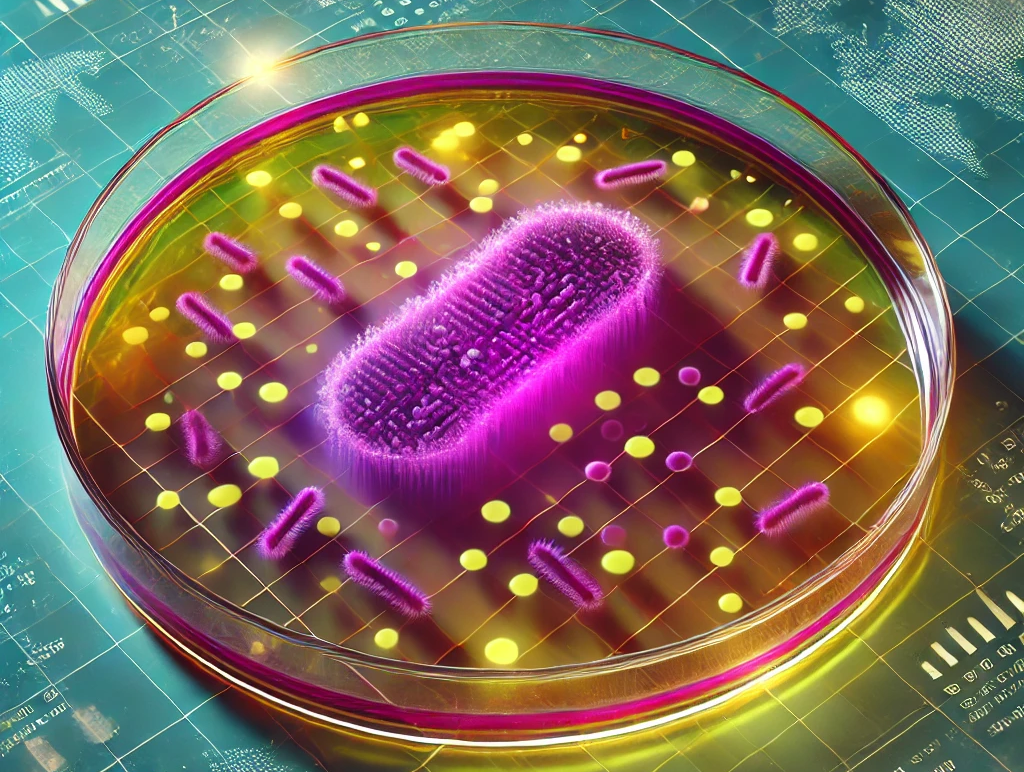
\includegraphics[width=0.8\textwidth,height=\textheight]{Modellering/figuren/ai_spatial.png}

}

\caption{Afbeelding gegenereerd met ChatGPT4-o}

\end{figure}

\hypertarget{leerdoelen-4}{%
\section{Leerdoelen}\label{leerdoelen-4}}

In dit hoofdstuk, gaan we na denken over hoe populaties (of het nu
bomen, bacteriën, of tumorcellen zijn) groeien in de ruimte. Dit doen we
door kennis te maken met \textbf{individual-based modelling}, wat
aanneemt dat organismen discrete individuen zijn, eventueel met hun
eigen omgeving en eigen gedragsregels. Aan het eind van dit hoofdstuk,
moet je begrijpen:

\begin{itemize}
\tightlist
\item
  Wat er bedoelt wordt met `omschrijvingsniveau'
\item
  Dat je naast populatiegroottes ook vanuit het individu kan denken
\item
  Dat interacties lokaal zijn, dus dat de posities van individuen ertoe
  kunnen doen
\item
  Hoe het komt dat sommige ruimtelijke modellen een ``ingebouwd''
  draagvlak hebben
\end{itemize}

\hypertarget{wat-is-individual-based-modelling}{%
\section{Wat is individual-based
modelling?}\label{wat-is-individual-based-modelling}}

Individual-based modelling (IBMs, ook wel \emph{agent-based modelling}
of ABMs genoemd), is een modeltechniek waarbij organismen als discrete
entiteiten (indivuen) worden beschouwd. Hierdoor kunnen we niet louter
en alleen populatiegroottes bestuderen, maar ook de eigenschappen en
gedragingen van individuen \emph{binnen} de populatie. Formeler gezegd
kunnen we stellen dat individual-based modellen een ander
\textbf{omschrijvingsniveau} hebben dan ODEs/differentievergelijkingen.
Dit omschrijvingsniveau bepaald ook welke \textbf{modeluitkomsten} we
kunnen verwachten: als we alleen de populatiegroottes bestuderen, kunnen
we geen inzichten over individuele verschillen verwachten! Laten we
hiermee kennis maken door te denken aan een bacteriekolonie die zich
over een agarplaat verspreidt.

\hypertarget{individuen-en-hun-posities}{%
\section{Individuen en hun posities}\label{individuen-en-hun-posities}}

Stel je voor dat in het midden van een agarplaat een enkele (paarse)
bacteriecel begint met delen (zie Figuur~\ref{fig-colony}). Deze cel
groeit met een bepaalde snelheid, en kan op een bepaald moment delen.
Maar reproductie is (meestal) een lokaal proces, dat wil zeggen, de
dochtercel zal naast de oudercel geplaatst worden. We kunnen ons dus
voorstellen dat, wanneer dit proces stap voor stap doorspeelt, de
kolonie bij benadering in een cirkelvorm zal uitgroeien. Als er ook een
kans is dat de dochtercel een mutatie heeft (waardoor deze bijvoorbeeld
geel wordt), dan ontstaat er over de tijd zelfs een interessant patroon
(zie Figuur~\ref{fig-colony}, rechter zijde). Door het perspectief in te
nemen van de cel (in plaats van de totale populatie), kunnen we dus gaan
nadenken over individuele verschillen in positie, kleur, groeisnelheid,
\emph{etc.}

\begin{Shaded}
\begin{Highlighting}[]
\CommentTok{\# Functie om het grid te visualiseren als punten}
\NormalTok{plot\_grid }\OtherTok{\textless{}{-}} \ControlFlowTok{function}\NormalTok{(grid) \{}
  \FunctionTok{par}\NormalTok{(}\AttributeTok{mar =} \FunctionTok{c}\NormalTok{(}\DecValTok{1}\NormalTok{, }\DecValTok{1}\NormalTok{, }\DecValTok{1}\NormalTok{, }\DecValTok{1}\NormalTok{))}
  \FunctionTok{plot}\NormalTok{(}\DecValTok{1}\NormalTok{, }\DecValTok{1}\NormalTok{, }\AttributeTok{type =} \StringTok{"n"}\NormalTok{, }\AttributeTok{xlim =} \FunctionTok{c}\NormalTok{(}\DecValTok{1}\NormalTok{, }\FunctionTok{nrow}\NormalTok{(grid)), }\AttributeTok{ylim =} \FunctionTok{c}\NormalTok{(}\DecValTok{1}\NormalTok{, }\FunctionTok{ncol}\NormalTok{(grid)), }\AttributeTok{xlab =} \StringTok{""}\NormalTok{, }\AttributeTok{ylab =} \StringTok{""}\NormalTok{, }\AttributeTok{axes =} \ConstantTok{FALSE}\NormalTok{, }\AttributeTok{asp =} \DecValTok{1}\NormalTok{)}
  
  \FunctionTok{points}\NormalTok{(}\FunctionTok{which}\NormalTok{(grid }\SpecialCharTok{==} \DecValTok{1}\NormalTok{, }\AttributeTok{arr.ind =} \ConstantTok{TRUE}\NormalTok{), }\AttributeTok{col =} \StringTok{"black"}\NormalTok{, }\AttributeTok{bg =} \StringTok{"purple"}\NormalTok{, }\AttributeTok{pch =} \DecValTok{21}\NormalTok{, }\AttributeTok{lwd=}\FloatTok{0.2}\NormalTok{, }\AttributeTok{cex =} \FloatTok{0.5}\NormalTok{)}
  \FunctionTok{points}\NormalTok{(}\FunctionTok{which}\NormalTok{(grid }\SpecialCharTok{==} \DecValTok{2}\NormalTok{, }\AttributeTok{arr.ind =} \ConstantTok{TRUE}\NormalTok{), }\AttributeTok{col =} \StringTok{"black"}\NormalTok{, }\AttributeTok{bg =} \StringTok{"gold"}\NormalTok{, }\AttributeTok{pch =} \DecValTok{21}\NormalTok{,}\AttributeTok{lwd=}\FloatTok{0.2}\NormalTok{, }\AttributeTok{cex =} \FloatTok{0.5}\NormalTok{)}
\NormalTok{\}}

\CommentTok{\# Functie om de groei{-}regels over het hele grid toe te passen. Deze regel werkt zo:}
\CommentTok{\# Voor elk lege punt (0), pak een }
\NormalTok{update\_grid }\OtherTok{\textless{}{-}} \ControlFlowTok{function}\NormalTok{(grid) \{}
\NormalTok{  size }\OtherTok{\textless{}{-}} \FunctionTok{nrow}\NormalTok{(grid)}
\NormalTok{  new\_grid }\OtherTok{\textless{}{-}}\NormalTok{ grid}
  
  \ControlFlowTok{for}\NormalTok{ (i }\ControlFlowTok{in} \DecValTok{1}\SpecialCharTok{:}\NormalTok{size) \{}
    \ControlFlowTok{for}\NormalTok{ (j }\ControlFlowTok{in} \DecValTok{1}\SpecialCharTok{:}\NormalTok{size) \{}
      \ControlFlowTok{if}\NormalTok{ (grid[i, j] }\SpecialCharTok{==} \DecValTok{1} \SpecialCharTok{||}\NormalTok{ grid[i, j] }\SpecialCharTok{==} \DecValTok{2}\NormalTok{) \{}
\NormalTok{        neighbors }\OtherTok{\textless{}{-}} \FunctionTok{cbind}\NormalTok{(}\FunctionTok{c}\NormalTok{(i}\DecValTok{{-}1}\NormalTok{, i}\SpecialCharTok{+}\DecValTok{1}\NormalTok{, i, i), }\FunctionTok{c}\NormalTok{(j, j, j}\DecValTok{{-}1}\NormalTok{, j}\SpecialCharTok{+}\DecValTok{1}\NormalTok{))}
        \ControlFlowTok{for}\NormalTok{ (k }\ControlFlowTok{in} \DecValTok{1}\SpecialCharTok{:}\FunctionTok{nrow}\NormalTok{(neighbors)) \{}
\NormalTok{          ni }\OtherTok{\textless{}{-}}\NormalTok{ neighbors[k, }\DecValTok{1}\NormalTok{]}
\NormalTok{          nj }\OtherTok{\textless{}{-}}\NormalTok{ neighbors[k, }\DecValTok{2}\NormalTok{]}
          \ControlFlowTok{if}\NormalTok{ (ni }\SpecialCharTok{\textgreater{}} \DecValTok{0} \SpecialCharTok{\&\&}\NormalTok{ ni }\SpecialCharTok{\textless{}=}\NormalTok{ size }\SpecialCharTok{\&\&}\NormalTok{ nj }\SpecialCharTok{\textgreater{}} \DecValTok{0} \SpecialCharTok{\&\&}\NormalTok{ nj }\SpecialCharTok{\textless{}=}\NormalTok{ size }\SpecialCharTok{\&\&}\NormalTok{ grid[ni, nj] }\SpecialCharTok{==} \DecValTok{0}\NormalTok{) \{}
            \ControlFlowTok{if}\NormalTok{ (}\FunctionTok{runif}\NormalTok{(}\DecValTok{1}\NormalTok{) }\SpecialCharTok{\textless{}} \FloatTok{0.5}\NormalTok{) \{  }\CommentTok{\# Geboortekans van 50\%}
\NormalTok{              new\_grid[ni, nj] }\OtherTok{\textless{}{-}}\NormalTok{ grid[i, j]  }\CommentTok{\# Kleur wordt overgedragen}
              \ControlFlowTok{if}\NormalTok{(}\FunctionTok{runif}\NormalTok{(}\DecValTok{1}\NormalTok{) }\SpecialCharTok{\textless{}} \FloatTok{0.01}\NormalTok{) grid[i,j] }\OtherTok{\textless{}{-}} \DecValTok{2}
\NormalTok{            \}}
\NormalTok{          \}}
\NormalTok{        \}}
\NormalTok{      \}}
\NormalTok{    \}}
\NormalTok{  \}}
  
  \FunctionTok{return}\NormalTok{(new\_grid)}
\NormalTok{\}}

\CommentTok{\# Maak een grid van 0{-}en met één 1tje in het midden}
\NormalTok{grid }\OtherTok{\textless{}{-}} \FunctionTok{matrix}\NormalTok{(}\DecValTok{0}\NormalTok{, }\AttributeTok{nrow =} \DecValTok{100}\NormalTok{, }\AttributeTok{ncol =} \DecValTok{100}\NormalTok{)}
\NormalTok{grid[}\DecValTok{50}\NormalTok{,}\DecValTok{50}\NormalTok{] }\OtherTok{\textless{}{-}} \DecValTok{1}
\FunctionTok{set.seed}\NormalTok{(}\DecValTok{59}\NormalTok{)}

\CommentTok{\# Loop om het grid bij te werken en te visualiseren}
\FunctionTok{layout}\NormalTok{(}\FunctionTok{matrix}\NormalTok{(}\FunctionTok{c}\NormalTok{(}\DecValTok{1}\NormalTok{,}\DecValTok{2}\NormalTok{,}\DecValTok{2}\NormalTok{,}\DecValTok{3}\NormalTok{,}\DecValTok{3}\NormalTok{,}\DecValTok{4}\NormalTok{,}\DecValTok{4}\NormalTok{),}\AttributeTok{nrow=}\DecValTok{1}\NormalTok{))}
\ControlFlowTok{for}\NormalTok{ (t }\ControlFlowTok{in} \DecValTok{1}\SpecialCharTok{:}\DecValTok{75}\NormalTok{) \{}
  \ControlFlowTok{if}\NormalTok{(t}\SpecialCharTok{==}\DecValTok{2} \SpecialCharTok{||}\NormalTok{ t}\SpecialCharTok{\%\%}\DecValTok{22}\SpecialCharTok{==}\DecValTok{0}\NormalTok{) }\FunctionTok{plot\_grid}\NormalTok{(grid)}
  \ControlFlowTok{if}\NormalTok{(t}\SpecialCharTok{==}\DecValTok{2}\NormalTok{) }\FunctionTok{arrows}\NormalTok{(}\DecValTok{20}\NormalTok{,}\DecValTok{20}\NormalTok{,}\DecValTok{40}\NormalTok{,}\DecValTok{40}\NormalTok{,}\AttributeTok{length=}\FloatTok{0.06}\NormalTok{,}\AttributeTok{lwd=}\DecValTok{2}\NormalTok{)}
\NormalTok{  grid }\OtherTok{\textless{}{-}} \FunctionTok{update\_grid}\NormalTok{(grid)}
  
  \FunctionTok{Sys.sleep}\NormalTok{(}\FloatTok{0.1}\NormalTok{)  }\CommentTok{\# Korte vertraging om de veranderingen zichtbaar te maken}
\NormalTok{\}}
\FunctionTok{title}\NormalTok{(}\StringTok{"Een groeiende bacteriekolonie met (gele) mutanten"}\NormalTok{, }\AttributeTok{cex.main=}\DecValTok{2}\NormalTok{,}\AttributeTok{line =} \SpecialCharTok{{-}}\DecValTok{2}\NormalTok{, }\AttributeTok{outer =} \ConstantTok{TRUE}\NormalTok{)}
\end{Highlighting}
\end{Shaded}

\begin{figure}[H]

{\centering 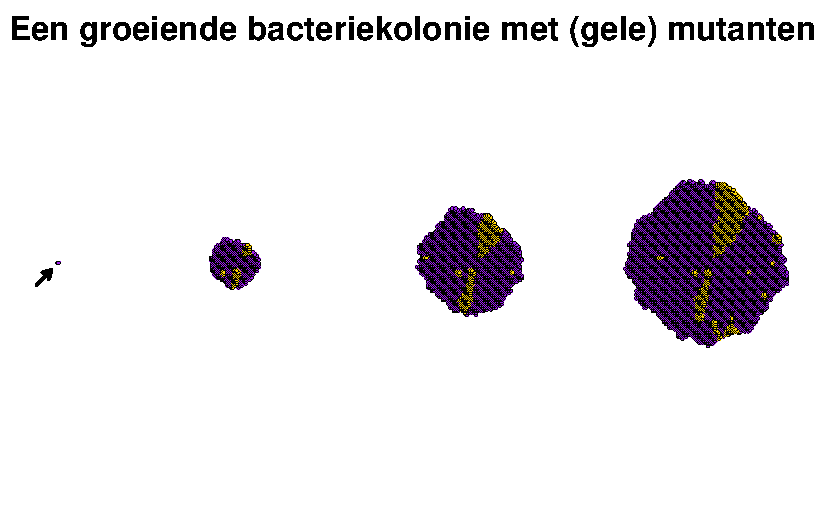
\includegraphics{Modellering/groei_ruimte_files/figure-pdf/fig-colony-1.pdf}

}

\caption{\label{fig-colony}Paarse stippen staan voor wildtye bacteriën,
terwjil gele stippen bacteriën zijn met een mutatie. Door lokale
celdeling onstaat er een ``taartpunt'' van mutanten, zoals waargenomen
in \href{https://www.nature.com/articles/ncomms12760}{Fusco et. al
(2016)}}

\end{figure}

De ruimtelijke structuur die in de IBM van Figuur
Figuur~\ref{fig-colony} ontstaat is een geheel \emph{nieuw} type
model-resultaat, en staat ons toe om vele nieuwe vragen te stellen: hoe
verspreiden mutaties zich in een bacteriekolonie? Hoe belangrijk is
zuurstof-beperking voor de groei van een tumor? Hoe behouden we diverse
ecosystemen wanneer bossen de heide overgroeien? Hoewel IBMs ook zonder
ruimtelijke structuur gemodelleerd kunnen worden, is dergelijke
structuur natuurlijk wel een belangrijk component van biologische
systemen! Maar hoe pakken we dat dan aan, individuen in de ruimte
modelleren?

\hypertarget{geboorte-in-lege-hokjes}{%
\section{Geboorte in ``lege hokjes''}\label{geboorte-in-lege-hokjes}}

Nu we het belang inzien van individuen en hun positie, hoe verwerken we
dit dan in een model? De meest eenvoudig vorm is wellicht een
2-dimensionale ruimte, waarin elk individu een x- en een y-coordinaat
heeft. We kunnen bijvoorbeeld een dataframe maken met daarin twee
individuen:

\begin{Shaded}
\begin{Highlighting}[]
\CommentTok{\# Maak twee individuen met een positie en een kleur}
\NormalTok{individual1 }\OtherTok{\textless{}{-}} \FunctionTok{data.frame}\NormalTok{(}\AttributeTok{x=}\DecValTok{6}\NormalTok{,}\AttributeTok{y=}\DecValTok{6}\NormalTok{,}\AttributeTok{col=}\StringTok{"brown"}\NormalTok{)}
\NormalTok{individual2 }\OtherTok{\textless{}{-}} \FunctionTok{data.frame}\NormalTok{(}\AttributeTok{x=}\DecValTok{7}\NormalTok{,}\AttributeTok{y=}\DecValTok{6}\NormalTok{,}\AttributeTok{col=}\StringTok{"orange"}\NormalTok{)}
\CommentTok{\# Zet ze samen in een dataframe als \textquotesingle{}beginpopulatie\textquotesingle{}}
\NormalTok{population }\OtherTok{\textless{}{-}} \FunctionTok{rbind}\NormalTok{(individual1, individual2)}
\NormalTok{population}
\end{Highlighting}
\end{Shaded}

\begin{verbatim}
  x y    col
1 6 6  brown
2 7 6 orange
\end{verbatim}

Om het extra simpel te houden, nemen we aan dat de x-y coordinaten
altijd gehele getallen zijn (\(x=1,2,3,\dots,S\) en
\(y=1,2,3,\dots,S\)), zodat we ons volledige ruimte kunnen voorstellen
als een simpel grid van hokjes (een soort schaakbord, maar dan zonder
die oneindige berg rijst). Nu zouden we elk individu in deze lijst
``regels'' kunnen geven voor hun voortplanting. Elk individu zou
bijvoorbeeld zich in een leeg buur-hokje kunnen voortplanten met een
kans van 60\%, en kunnen sterven met een kans van 5\%. Laten we even
stellen dat de kleur van het individu niet uitmaakt voor deze regels:
deze is alleen voor de visualisatie. Als we dit simuleren in R, zouden
we zoiets kunnen zien:

\begin{Shaded}
\begin{Highlighting}[]
\CommentTok{\# Maak een 12x12 grid}
\NormalTok{grid\_size }\OtherTok{\textless{}{-}} \DecValTok{12}
\NormalTok{grid }\OtherTok{\textless{}{-}} \FunctionTok{matrix}\NormalTok{(}\DecValTok{0}\NormalTok{, }\AttributeTok{nrow =}\NormalTok{ grid\_size, }\AttributeTok{ncol =}\NormalTok{ grid\_size)}
\CommentTok{\# Maak twee individuen met een positie en een kleur}
\NormalTok{individual1 }\OtherTok{\textless{}{-}} \FunctionTok{data.frame}\NormalTok{(}\AttributeTok{x=}\DecValTok{6}\NormalTok{,}\AttributeTok{y=}\DecValTok{6}\NormalTok{,}\AttributeTok{col=}\StringTok{"brown"}\NormalTok{)}
\NormalTok{individual2 }\OtherTok{\textless{}{-}} \FunctionTok{data.frame}\NormalTok{(}\AttributeTok{x=}\DecValTok{7}\NormalTok{,}\AttributeTok{y=}\DecValTok{6}\NormalTok{,}\AttributeTok{col=}\StringTok{"orange"}\NormalTok{)}
\CommentTok{\# Zet ze samen in een dataframe als \textquotesingle{}mbeginpopulatie\textquotesingle{}}
\NormalTok{population }\OtherTok{\textless{}{-}} \FunctionTok{rbind}\NormalTok{(individual1, individual2)}
\NormalTok{grid[}\DecValTok{6}\NormalTok{, }\DecValTok{6}\NormalTok{] }\OtherTok{\textless{}{-}} \DecValTok{1} \CommentTok{\# 6,6 zit vol}
\NormalTok{grid[}\DecValTok{6}\NormalTok{, }\DecValTok{7}\NormalTok{] }\OtherTok{\textless{}{-}} \DecValTok{1} \CommentTok{\# 7,6 zit vol (let op dat row=y en col=x)}

\CommentTok{\# Groei{-}simulatie functie}
\NormalTok{simulate\_growth }\OtherTok{\textless{}{-}} \ControlFlowTok{function}\NormalTok{(}\AttributeTok{geboorte =} \FloatTok{0.6}\NormalTok{, }\AttributeTok{sterfte=}\FloatTok{0.1}\NormalTok{) \{}
\NormalTok{  deaths }\OtherTok{\textless{}{-}} \FunctionTok{c}\NormalTok{() }\CommentTok{\# Houd bij wie er dood gaan, zodat deze aan het einde uit de populatie gehaald kunnen worden}
  \ControlFlowTok{for}\NormalTok{ (i }\ControlFlowTok{in} \DecValTok{1}\SpecialCharTok{:}\FunctionTok{nrow}\NormalTok{(population)) \{}
\NormalTok{    ind }\OtherTok{\textless{}{-}}\NormalTok{ population[i,]}
    \ControlFlowTok{if}\NormalTok{(}\FunctionTok{runif}\NormalTok{(}\DecValTok{1}\NormalTok{) }\SpecialCharTok{\textless{}}\NormalTok{ geboorte)\{}
\NormalTok{      new\_x }\OtherTok{\textless{}{-}}\NormalTok{ ind}\SpecialCharTok{$}\NormalTok{x }\SpecialCharTok{+} \FunctionTok{sample}\NormalTok{(}\FunctionTok{c}\NormalTok{(}\SpecialCharTok{{-}}\DecValTok{1}\SpecialCharTok{:}\DecValTok{1}\NormalTok{),}\DecValTok{1}\NormalTok{)}
\NormalTok{      new\_y }\OtherTok{\textless{}{-}}\NormalTok{ ind}\SpecialCharTok{$}\NormalTok{y }\SpecialCharTok{+} \FunctionTok{sample}\NormalTok{(}\FunctionTok{c}\NormalTok{(}\SpecialCharTok{{-}}\DecValTok{1}\SpecialCharTok{:}\DecValTok{1}\NormalTok{),}\DecValTok{1}\NormalTok{)}
      \ControlFlowTok{if}\NormalTok{(new\_x}\SpecialCharTok{\textless{}}\DecValTok{1} \SpecialCharTok{||}\NormalTok{ new\_x }\SpecialCharTok{\textgreater{}}\NormalTok{ grid\_size }\SpecialCharTok{||}\NormalTok{ new\_y }\SpecialCharTok{\textless{}} \DecValTok{1} \SpecialCharTok{||}\NormalTok{ new\_y }\SpecialCharTok{\textgreater{}}\NormalTok{ grid\_size) }\ControlFlowTok{next}
      \ControlFlowTok{if}\NormalTok{(grid[new\_y,new\_x] }\SpecialCharTok{==} \DecValTok{0}\NormalTok{)\{}
\NormalTok{        grid[new\_y,new\_x] }\OtherTok{\textless{}\textless{}{-}} \DecValTok{1}
\NormalTok{        population }\OtherTok{\textless{}\textless{}{-}} \FunctionTok{rbind}\NormalTok{(population,}\FunctionTok{data.frame}\NormalTok{(}\AttributeTok{x=}\NormalTok{new\_x,}\AttributeTok{y=}\NormalTok{new\_y,}\AttributeTok{col=}\NormalTok{ind}\SpecialCharTok{$}\NormalTok{col))}
\NormalTok{      \}}
\NormalTok{    \}}
    \ControlFlowTok{if}\NormalTok{(}\FunctionTok{runif}\NormalTok{(}\DecValTok{1}\NormalTok{) }\SpecialCharTok{\textless{}}\NormalTok{ sterfte)\{}
\NormalTok{      grid[ind}\SpecialCharTok{$}\NormalTok{y,ind}\SpecialCharTok{$}\NormalTok{x] }\OtherTok{\textless{}\textless{}{-}} \DecValTok{0}
\NormalTok{      deaths }\OtherTok{\textless{}{-}} \FunctionTok{c}\NormalTok{(deaths, i)}
\NormalTok{    \}}
\NormalTok{  \}}
  \ControlFlowTok{if}\NormalTok{(}\FunctionTok{length}\NormalTok{(deaths) }\SpecialCharTok{\textgreater{}} \DecValTok{0}\NormalTok{) population }\OtherTok{\textless{}\textless{}{-}}\NormalTok{ population[}\SpecialCharTok{{-}}\NormalTok{deaths,]}
\NormalTok{\}}

\CommentTok{\# Functie om het grid als bruine stipjes op een grid te plotten. }
\NormalTok{plot\_grid }\OtherTok{\textless{}{-}} \ControlFlowTok{function}\NormalTok{(grid, time) \{}
  \FunctionTok{plot}\NormalTok{(}\DecValTok{1}\SpecialCharTok{:}\NormalTok{grid\_size, }\DecValTok{1}\SpecialCharTok{:}\NormalTok{grid\_size, }\AttributeTok{type =} \StringTok{"n"}\NormalTok{, }\AttributeTok{xlab =} \StringTok{""}\NormalTok{, }\AttributeTok{ylab =} \StringTok{""}\NormalTok{, }\AttributeTok{axes =} \ConstantTok{FALSE}\NormalTok{)}
  \CommentTok{\# Grijze lijntjes}
  \ControlFlowTok{for}\NormalTok{ (i }\ControlFlowTok{in} \DecValTok{0}\SpecialCharTok{:}\NormalTok{(grid\_size)}\SpecialCharTok{+}\DecValTok{1}\NormalTok{) \{}
    \FunctionTok{abline}\NormalTok{(}\AttributeTok{h =}\NormalTok{ i}\FloatTok{{-}0.5}\NormalTok{, }\AttributeTok{col =} \StringTok{"grey"}\NormalTok{, }\AttributeTok{lty =} \DecValTok{1}\NormalTok{)}
    \FunctionTok{abline}\NormalTok{(}\AttributeTok{v =}\NormalTok{ i}\FloatTok{{-}0.5}\NormalTok{, }\AttributeTok{col =} \StringTok{"grey"}\NormalTok{, }\AttributeTok{lty =} \DecValTok{1}\NormalTok{)}
\NormalTok{  \}}
  \CommentTok{\# Bruine stipjes}
  \ControlFlowTok{for}\NormalTok{ (i }\ControlFlowTok{in} \DecValTok{1}\SpecialCharTok{:}\FunctionTok{nrow}\NormalTok{(population)) \{}
\NormalTok{    ind }\OtherTok{\textless{}{-}}\NormalTok{ population[i,]}
    \FunctionTok{points}\NormalTok{(ind}\SpecialCharTok{$}\NormalTok{x, ind}\SpecialCharTok{$}\NormalTok{y, }\AttributeTok{pch =} \DecValTok{16}\NormalTok{, }\AttributeTok{col =}\NormalTok{ ind}\SpecialCharTok{$}\NormalTok{col)}
\NormalTok{  \}}
  \FunctionTok{title}\NormalTok{(}\FunctionTok{paste}\NormalTok{(}\StringTok{"Tijdstap"}\NormalTok{,time))}
\NormalTok{\}}

\CommentTok{\# Start een random nummer generator (gerandeert reproduceerbaarheid)}
\CommentTok{\#set.seed(591)}

\FunctionTok{par}\NormalTok{(}\AttributeTok{mfrow=}\FunctionTok{c}\NormalTok{(}\DecValTok{3}\NormalTok{,}\DecValTok{5}\NormalTok{),}\AttributeTok{mar=}\FunctionTok{c}\NormalTok{(}\DecValTok{1}\NormalTok{,}\DecValTok{1}\NormalTok{,}\DecValTok{2}\NormalTok{,}\DecValTok{2}\NormalTok{))}
\CommentTok{\# Simuleer een x{-}aantal tijdstappen (x=iterations)}
\NormalTok{iterations }\OtherTok{\textless{}{-}} \DecValTok{28}
\FunctionTok{plot\_grid}\NormalTok{(grid,}\DecValTok{0}\NormalTok{)}
\ControlFlowTok{for}\NormalTok{ (i }\ControlFlowTok{in} \DecValTok{1}\SpecialCharTok{:}\NormalTok{iterations) \{}
  \ControlFlowTok{if}\NormalTok{(i}\SpecialCharTok{\%\%}\DecValTok{2}\SpecialCharTok{==}\DecValTok{0}\NormalTok{) }\FunctionTok{plot\_grid}\NormalTok{(grid,i)}
  \FunctionTok{simulate\_growth}\NormalTok{(}\FloatTok{0.6}\NormalTok{, }\FloatTok{0.1}\NormalTok{)}
\NormalTok{\}}
\end{Highlighting}
\end{Shaded}

\begin{figure}[H]

{\centering 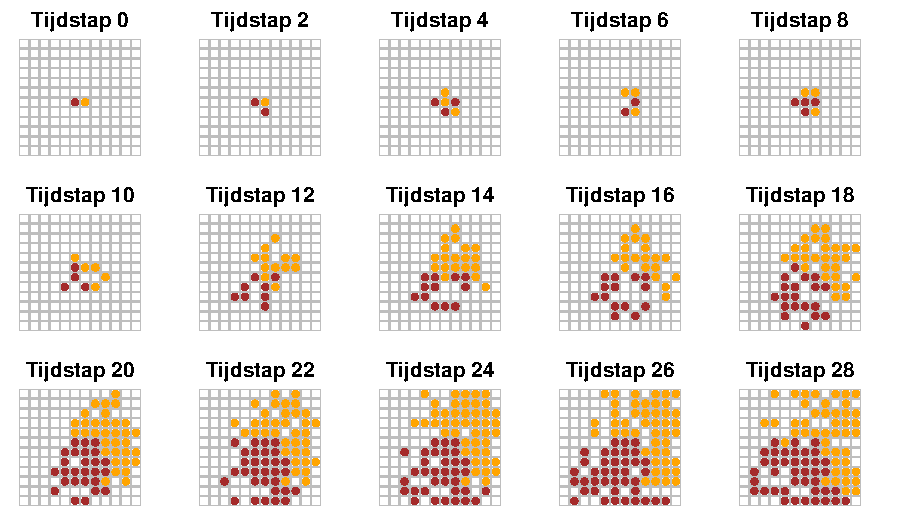
\includegraphics{Modellering/groei_ruimte_files/figure-pdf/fig-simgrowthgrid222-1.pdf}

}

\caption{\label{fig-simgrowthgrid222}Simulatie van groei op een grid,
waarbij ``individuen'' kunnen reproduceren in lege buur-hokjes met een
kans van 60\%, en sterven met een vaste kans van 5\%. De kleur heeft
hier geen invloed op, en dient alleen ter illustratie.}

\end{figure}

Hoewel het R-script geen dichtheidsafhankelijke afname van de
geboortekans gebruikt (deze blijft altijd 60\%), zal de populatie toch
niet meer toenemen zodra het grid vol zit. De reden dat er toch een
draagvlak aanwezig is, is simpelweg doordat individuen alleen kunnen
voortplanten in \emph{lege} hokjes. De \emph{daadwerkelijke}
geboortekans is dus helemaal niet constant, want op een vol grid is die
veel kleiner dan op een leeg grid! Als we hadden aangenomen dat
individuen ook kunnen voortplanten in bezette hokjes, dan zou de
populatie inderdaad exponentiëel blijven groeien.

\begin{tcolorbox}[enhanced jigsaw, coltitle=black, breakable, bottomtitle=1mm, opacityback=0, colback=white, rightrule=.15mm, title=\textcolor{quarto-callout-tip-color}{\faLightbulb}\hspace{0.5em}{Is ruimte beperkend voor groei?}, bottomrule=.15mm, toprule=.15mm, left=2mm, colframe=quarto-callout-tip-color-frame, toptitle=1mm, opacitybacktitle=0.6, titlerule=0mm, colbacktitle=quarto-callout-tip-color!10!white, leftrule=.75mm, arc=.35mm]

De aanname dat ruimte een intrinsieke beperking is voor groei hangt
sterk af van het biologische scenario: voor planten die licht moeten
opvangen geldt dit waarschijnlijk wel, maar voor de grazers die deze
planten eten wellicht niet. Vergelijkbaar hebben bacteriën op een
agarplaat of tumorcellen alleen voedingsstoffen aan de rand, wat een
vergelijkbaar effect oplevert waarbij er alleen in ``lege ruimte'' groei
mogelijk is. Dergelijke overwegingen zijn heel belangrijk als we
biologische systemen goed willen kunnen voorspellen!

\end{tcolorbox}

Een ander belangrijk verschil met onze eerdere (wiskundige) modellen is
dat we nu gebruik maken van \textbf{stochasticiteit}, dat wil zeggen
kansprocessen. Specifieker zijn birth en death zijn geen snelheden meer,
maar kansprocessen. Als in deze simulatie birth veel hoger is dan death
(\(b\gg d\)), zal de populatie natuurlijk gewoon uitgroeien totdat een
groot deel van het grid vol zit (Figuur~\ref{fig-stochasticity-1}).
Daarna zal de populatie een beetje rond een evenwicht fluctueren,
waarbij death wordt gecompenseerd door birth.

Wanneer het verschil tussen \(b\) en \(d\) veel kleiner is, groeit het
grid minder vol.~Ook zie je dat de fluctuaties rond het evenwicht wat
sterker zijn geworden (Figuur~\ref{fig-stochasticity-2}). Daarnaast zie
je in deze simulatie dat er aan het einde, door toeval, alleen nog
oranje individuen over zijn!

Als \(b\) slechts een klein beetje groter is dan \(d\)
(Figuur~\ref{fig-stochasticity-3}), zien we zelfs dat de kleine
start-populatie van 2 cellen door stomme pech uit zou kunnen sterven.
Ook dit was niet mogelijk in de ODEs, waar \(b>d\) altijd exponentiële
groei geeft.

\begin{Shaded}
\begin{Highlighting}[]
\CommentTok{\# Maak een 12x12 grid}
\NormalTok{grid\_size }\OtherTok{\textless{}{-}} \DecValTok{32}
\NormalTok{grid }\OtherTok{\textless{}{-}} \FunctionTok{matrix}\NormalTok{(}\DecValTok{0}\NormalTok{, }\AttributeTok{nrow =}\NormalTok{ grid\_size, }\AttributeTok{ncol =}\NormalTok{ grid\_size)}
\CommentTok{\# Maak twee individuen met een positie en een kleur}
\NormalTok{individual1 }\OtherTok{\textless{}{-}} \FunctionTok{data.frame}\NormalTok{(}\AttributeTok{x=}\DecValTok{16}\NormalTok{,}\AttributeTok{y=}\DecValTok{16}\NormalTok{,}\AttributeTok{col=}\StringTok{"brown"}\NormalTok{)}
\NormalTok{individual2 }\OtherTok{\textless{}{-}} \FunctionTok{data.frame}\NormalTok{(}\AttributeTok{x=}\DecValTok{17}\NormalTok{,}\AttributeTok{y=}\DecValTok{16}\NormalTok{,}\AttributeTok{col=}\StringTok{"orange"}\NormalTok{)}
\CommentTok{\# Zet ze samen in een dataframe als \textquotesingle{}mbeginpopulatie\textquotesingle{}}
\NormalTok{population }\OtherTok{\textless{}{-}} \FunctionTok{rbind}\NormalTok{(individual1, individual2)}
\NormalTok{grid[}\DecValTok{16}\NormalTok{, }\DecValTok{16}\NormalTok{] }\OtherTok{\textless{}{-}} \DecValTok{1} \CommentTok{\# 6,6 zit vol}
\NormalTok{grid[}\DecValTok{16}\NormalTok{, }\DecValTok{17}\NormalTok{] }\OtherTok{\textless{}{-}} \DecValTok{1} \CommentTok{\# 7,6 zit vol (let op dat row=y en col=x)}

\CommentTok{\# Groei{-}simulatie functie}
\NormalTok{simulate\_growth }\OtherTok{\textless{}{-}} \ControlFlowTok{function}\NormalTok{(}\AttributeTok{geboorte =} \FloatTok{0.6}\NormalTok{, }\AttributeTok{sterfte=}\FloatTok{0.1}\NormalTok{) \{}
\NormalTok{  deaths }\OtherTok{\textless{}{-}} \FunctionTok{c}\NormalTok{() }\CommentTok{\# Houd bij wie er dood gaan, zodat deze aan het einde uit de populatie gehaald kunnen worden}
  \ControlFlowTok{for}\NormalTok{ (i }\ControlFlowTok{in} \DecValTok{1}\SpecialCharTok{:}\FunctionTok{nrow}\NormalTok{(population)) \{}
\NormalTok{    ind }\OtherTok{\textless{}{-}}\NormalTok{ population[i,]}
    \ControlFlowTok{if}\NormalTok{(}\FunctionTok{runif}\NormalTok{(}\DecValTok{1}\NormalTok{) }\SpecialCharTok{\textless{}}\NormalTok{ geboorte)\{}
\NormalTok{      new\_x }\OtherTok{\textless{}{-}}\NormalTok{ ind}\SpecialCharTok{$}\NormalTok{x }\SpecialCharTok{+} \FunctionTok{sample}\NormalTok{(}\FunctionTok{c}\NormalTok{(}\SpecialCharTok{{-}}\DecValTok{1}\SpecialCharTok{:}\DecValTok{1}\NormalTok{),}\DecValTok{1}\NormalTok{)}
\NormalTok{      new\_y }\OtherTok{\textless{}{-}}\NormalTok{ ind}\SpecialCharTok{$}\NormalTok{y }\SpecialCharTok{+} \FunctionTok{sample}\NormalTok{(}\FunctionTok{c}\NormalTok{(}\SpecialCharTok{{-}}\DecValTok{1}\SpecialCharTok{:}\DecValTok{1}\NormalTok{),}\DecValTok{1}\NormalTok{)}
      \ControlFlowTok{if}\NormalTok{(new\_x}\SpecialCharTok{\textless{}}\DecValTok{1} \SpecialCharTok{||}\NormalTok{ new\_x }\SpecialCharTok{\textgreater{}}\NormalTok{ grid\_size }\SpecialCharTok{||}\NormalTok{ new\_y }\SpecialCharTok{\textless{}} \DecValTok{1} \SpecialCharTok{||}\NormalTok{ new\_y }\SpecialCharTok{\textgreater{}}\NormalTok{ grid\_size) }\ControlFlowTok{next}
      \ControlFlowTok{if}\NormalTok{(grid[new\_y,new\_x] }\SpecialCharTok{==} \DecValTok{0}\NormalTok{)\{}
\NormalTok{        grid[new\_y,new\_x] }\OtherTok{\textless{}\textless{}{-}} \DecValTok{1}
\NormalTok{        population }\OtherTok{\textless{}\textless{}{-}} \FunctionTok{rbind}\NormalTok{(population,}\FunctionTok{data.frame}\NormalTok{(}\AttributeTok{x=}\NormalTok{new\_x,}\AttributeTok{y=}\NormalTok{new\_y,}\AttributeTok{col=}\NormalTok{ind}\SpecialCharTok{$}\NormalTok{col))}
\NormalTok{      \}}
\NormalTok{    \}}
    \ControlFlowTok{if}\NormalTok{(}\FunctionTok{runif}\NormalTok{(}\DecValTok{1}\NormalTok{) }\SpecialCharTok{\textless{}}\NormalTok{ sterfte)\{}
\NormalTok{      grid[ind}\SpecialCharTok{$}\NormalTok{y,ind}\SpecialCharTok{$}\NormalTok{x] }\OtherTok{\textless{}\textless{}{-}} \DecValTok{0}
\NormalTok{      deaths }\OtherTok{\textless{}{-}} \FunctionTok{c}\NormalTok{(deaths, i)}
\NormalTok{    \}}
\NormalTok{  \}}
  \ControlFlowTok{if}\NormalTok{(}\FunctionTok{length}\NormalTok{(deaths) }\SpecialCharTok{\textgreater{}} \DecValTok{0}\NormalTok{) population }\OtherTok{\textless{}\textless{}{-}}\NormalTok{ population[}\SpecialCharTok{{-}}\NormalTok{deaths,]}
\NormalTok{\}}

\CommentTok{\# Functie om het grid als bruine stipjes op een grid te plotten. }
\NormalTok{plot\_grid }\OtherTok{\textless{}{-}} \ControlFlowTok{function}\NormalTok{(grid, time) \{}
  \FunctionTok{plot}\NormalTok{(}\DecValTok{1}\SpecialCharTok{:}\NormalTok{grid\_size, }\DecValTok{1}\SpecialCharTok{:}\NormalTok{grid\_size, }\AttributeTok{type =} \StringTok{"n"}\NormalTok{, }\AttributeTok{xlab =} \StringTok{""}\NormalTok{, }\AttributeTok{ylab =} \StringTok{""}\NormalTok{, }\AttributeTok{axes =} \ConstantTok{FALSE}\NormalTok{)}
  \CommentTok{\# Grijze lijntjes}
  \ControlFlowTok{for}\NormalTok{ (i }\ControlFlowTok{in} \DecValTok{0}\SpecialCharTok{:}\NormalTok{(grid\_size)}\SpecialCharTok{+}\DecValTok{1}\NormalTok{) \{}
    \FunctionTok{abline}\NormalTok{(}\AttributeTok{h =}\NormalTok{ i}\FloatTok{{-}0.5}\NormalTok{, }\AttributeTok{col =} \StringTok{"grey"}\NormalTok{, }\AttributeTok{lty =} \DecValTok{1}\NormalTok{)}
    \FunctionTok{abline}\NormalTok{(}\AttributeTok{v =}\NormalTok{ i}\FloatTok{{-}0.5}\NormalTok{, }\AttributeTok{col =} \StringTok{"grey"}\NormalTok{, }\AttributeTok{lty =} \DecValTok{1}\NormalTok{)}
\NormalTok{  \}}
  \CommentTok{\# Bruine stipjes}
  \ControlFlowTok{for}\NormalTok{ (i }\ControlFlowTok{in} \DecValTok{1}\SpecialCharTok{:}\FunctionTok{nrow}\NormalTok{(population)) \{}
\NormalTok{    ind }\OtherTok{\textless{}{-}}\NormalTok{ population[i,]}
    \FunctionTok{points}\NormalTok{(ind}\SpecialCharTok{$}\NormalTok{x, ind}\SpecialCharTok{$}\NormalTok{y, }\AttributeTok{pch =} \DecValTok{16}\NormalTok{, }\AttributeTok{col =}\NormalTok{ ind}\SpecialCharTok{$}\NormalTok{col,}\AttributeTok{cex =} \DecValTok{1}\NormalTok{)}
\NormalTok{  \}}
  \FunctionTok{title}\NormalTok{(}\FunctionTok{paste0}\NormalTok{(}\StringTok{"Grid op t="}\NormalTok{,time))}
\NormalTok{\}}

\CommentTok{\# Start een random nummer generator (gerandeert reproduceerbaarheid)}
\FunctionTok{set.seed}\NormalTok{(}\DecValTok{596}\NormalTok{)}
\CommentTok{\#par(mfrow=c(1,2),mar=c(3,3,1,1))}
\NormalTok{layout.matrix }\OtherTok{\textless{}{-}} \FunctionTok{matrix}\NormalTok{(}\FunctionTok{c}\NormalTok{(}\DecValTok{1}\NormalTok{, }\DecValTok{2}\NormalTok{), }\AttributeTok{nrow =} \DecValTok{1}\NormalTok{, }\AttributeTok{ncol =} \DecValTok{2}\NormalTok{)}
\FunctionTok{layout}\NormalTok{(}\AttributeTok{mat =}\NormalTok{ layout.matrix, }\AttributeTok{widths=}\FunctionTok{c}\NormalTok{(}\FloatTok{2.5}\NormalTok{,}\DecValTok{1}\NormalTok{))}
\FunctionTok{par}\NormalTok{(}\AttributeTok{mar=}\FunctionTok{c}\NormalTok{(}\DecValTok{4}\NormalTok{,}\DecValTok{4}\NormalTok{,}\DecValTok{1}\NormalTok{,}\DecValTok{1}\NormalTok{))}
\NormalTok{population }\OtherTok{\textless{}{-}} \FunctionTok{rbind}\NormalTok{(individual1, individual2)}
\NormalTok{grid }\OtherTok{\textless{}{-}} \FunctionTok{matrix}\NormalTok{(}\DecValTok{0}\NormalTok{, }\AttributeTok{nrow =}\NormalTok{ grid\_size, }\AttributeTok{ncol =}\NormalTok{ grid\_size)}
\NormalTok{grid[}\DecValTok{16}\NormalTok{, }\DecValTok{16}\NormalTok{] }\OtherTok{\textless{}{-}} \DecValTok{1} \CommentTok{\# 6,6 zit vol}
\NormalTok{grid[}\DecValTok{16}\NormalTok{, }\DecValTok{17}\NormalTok{] }\OtherTok{\textless{}{-}} \DecValTok{1} \CommentTok{\# 7,6 zit vol (let op dat row=y en col=x)}
\CommentTok{\# Simuleer een x{-}aantal tijdstappen (x=iterations)}
\NormalTok{iterations }\OtherTok{\textless{}{-}} \DecValTok{300}
\NormalTok{popsize }\OtherTok{\textless{}{-}} \FunctionTok{nrow}\NormalTok{(population)}
\ControlFlowTok{for}\NormalTok{ (i }\ControlFlowTok{in} \DecValTok{1}\SpecialCharTok{:}\NormalTok{iterations) \{}
  \FunctionTok{simulate\_growth}\NormalTok{(}\FloatTok{0.6}\NormalTok{, }\FloatTok{0.1}\NormalTok{)}
\NormalTok{  popsize[i}\SpecialCharTok{+}\DecValTok{1}\NormalTok{] }\OtherTok{\textless{}{-}} \FunctionTok{nrow}\NormalTok{(population)}
\NormalTok{\}}
\FunctionTok{ts.plot}\NormalTok{(popsize, }\AttributeTok{xlab=}\StringTok{"Tijd"}\NormalTok{, }\AttributeTok{ylab=}\StringTok{"Populatiegrootte"}\NormalTok{, }\AttributeTok{lwd=}\DecValTok{2}\NormalTok{, }\AttributeTok{main=}\StringTok{""}\NormalTok{)}
\FunctionTok{par}\NormalTok{(}\AttributeTok{mar=}\FunctionTok{c}\NormalTok{(}\DecValTok{1}\NormalTok{,}\DecValTok{1}\NormalTok{,}\DecValTok{1}\NormalTok{,}\DecValTok{1}\NormalTok{))}
\FunctionTok{plot\_grid}\NormalTok{(population,}\DecValTok{300}\NormalTok{)}

\FunctionTok{par}\NormalTok{(}\AttributeTok{mar=}\FunctionTok{c}\NormalTok{(}\DecValTok{4}\NormalTok{,}\DecValTok{4}\NormalTok{,}\DecValTok{1}\NormalTok{,}\DecValTok{1}\NormalTok{))}
\NormalTok{population }\OtherTok{\textless{}{-}} \FunctionTok{rbind}\NormalTok{(individual1, individual2)}
\NormalTok{grid }\OtherTok{\textless{}{-}} \FunctionTok{matrix}\NormalTok{(}\DecValTok{0}\NormalTok{, }\AttributeTok{nrow =}\NormalTok{ grid\_size, }\AttributeTok{ncol =}\NormalTok{ grid\_size)}
\NormalTok{grid[}\DecValTok{16}\NormalTok{, }\DecValTok{16}\NormalTok{] }\OtherTok{\textless{}{-}} \DecValTok{1} \CommentTok{\# 6,6 zit vol}
\NormalTok{grid[}\DecValTok{16}\NormalTok{, }\DecValTok{17}\NormalTok{] }\OtherTok{\textless{}{-}} \DecValTok{1} \CommentTok{\# 7,6 zit vol (let op dat row=y en col=x)}
\CommentTok{\# Simuleer een x{-}aantal tijdstappen (x=iterations)}
\NormalTok{iterations }\OtherTok{\textless{}{-}} \DecValTok{300}
\NormalTok{popsize }\OtherTok{\textless{}{-}} \FunctionTok{nrow}\NormalTok{(population)}
\ControlFlowTok{for}\NormalTok{ (i }\ControlFlowTok{in} \DecValTok{1}\SpecialCharTok{:}\NormalTok{iterations) \{}
  \FunctionTok{simulate\_growth}\NormalTok{(}\FloatTok{0.3}\NormalTok{, }\FloatTok{0.1}\NormalTok{)}
\NormalTok{  popsize[i}\SpecialCharTok{+}\DecValTok{1}\NormalTok{] }\OtherTok{\textless{}{-}} \FunctionTok{nrow}\NormalTok{(population)}
\NormalTok{\}}
\FunctionTok{ts.plot}\NormalTok{(popsize, }\AttributeTok{xlab=}\StringTok{"Tijd"}\NormalTok{, }\AttributeTok{ylab=}\StringTok{"Populatiegrootte"}\NormalTok{, }\AttributeTok{lwd=}\DecValTok{2}\NormalTok{, }\AttributeTok{main=}\StringTok{""}\NormalTok{)}
\FunctionTok{par}\NormalTok{(}\AttributeTok{mar=}\FunctionTok{c}\NormalTok{(}\DecValTok{1}\NormalTok{,}\DecValTok{1}\NormalTok{,}\DecValTok{1}\NormalTok{,}\DecValTok{1}\NormalTok{))}
\FunctionTok{plot\_grid}\NormalTok{(population,}\DecValTok{300}\NormalTok{)}

\FunctionTok{par}\NormalTok{(}\AttributeTok{mar=}\FunctionTok{c}\NormalTok{(}\DecValTok{4}\NormalTok{,}\DecValTok{4}\NormalTok{,}\DecValTok{1}\NormalTok{,}\DecValTok{1}\NormalTok{))}
\NormalTok{population }\OtherTok{\textless{}{-}} \FunctionTok{rbind}\NormalTok{(individual1, individual2)}
\NormalTok{grid }\OtherTok{\textless{}{-}} \FunctionTok{matrix}\NormalTok{(}\DecValTok{0}\NormalTok{, }\AttributeTok{nrow =}\NormalTok{ grid\_size, }\AttributeTok{ncol =}\NormalTok{ grid\_size)}
\NormalTok{grid[}\DecValTok{16}\NormalTok{, }\DecValTok{16}\NormalTok{] }\OtherTok{\textless{}{-}} \DecValTok{1} \CommentTok{\# 6,6 zit vol}
\NormalTok{grid[}\DecValTok{16}\NormalTok{, }\DecValTok{17}\NormalTok{] }\OtherTok{\textless{}{-}} \DecValTok{1} \CommentTok{\# 7,6 zit vol (let op dat row=y en col=x)}
\CommentTok{\# Simuleer een x{-}aantal tijdstappen (x=iterations)}
\NormalTok{iterations }\OtherTok{\textless{}{-}} \DecValTok{300}
\NormalTok{popsize }\OtherTok{\textless{}{-}} \FunctionTok{nrow}\NormalTok{(population)}
\ControlFlowTok{for}\NormalTok{ (i }\ControlFlowTok{in} \DecValTok{1}\SpecialCharTok{:}\NormalTok{iterations) \{}
  \FunctionTok{simulate\_growth}\NormalTok{(}\FloatTok{0.12}\NormalTok{, }\FloatTok{0.1}\NormalTok{)}
\NormalTok{  popsize[i}\SpecialCharTok{+}\DecValTok{1}\NormalTok{] }\OtherTok{\textless{}{-}} \FunctionTok{nrow}\NormalTok{(population)}
  \ControlFlowTok{if}\NormalTok{(popsize[i}\SpecialCharTok{+}\DecValTok{1}\NormalTok{]}\SpecialCharTok{==}\DecValTok{0}\NormalTok{) }\ControlFlowTok{break}
\NormalTok{\}}
\FunctionTok{ts.plot}\NormalTok{(popsize, }\AttributeTok{xlab=}\StringTok{"Tijd"}\NormalTok{, }\AttributeTok{ylab=}\StringTok{"Populatiegrootte"}\NormalTok{, }\AttributeTok{lwd=}\DecValTok{2}\NormalTok{, }\AttributeTok{main=}\StringTok{""}\NormalTok{)}
\FunctionTok{par}\NormalTok{(}\AttributeTok{mar=}\FunctionTok{c}\NormalTok{(}\DecValTok{1}\NormalTok{,}\DecValTok{1}\NormalTok{,}\DecValTok{1}\NormalTok{,}\DecValTok{1}\NormalTok{))}
\FunctionTok{plot\_grid}\NormalTok{(population,}\DecValTok{300}\NormalTok{)}
\end{Highlighting}
\end{Shaded}

\begin{figure}

\begin{minipage}[t]{\linewidth}

{\centering 

\raisebox{-\height}{

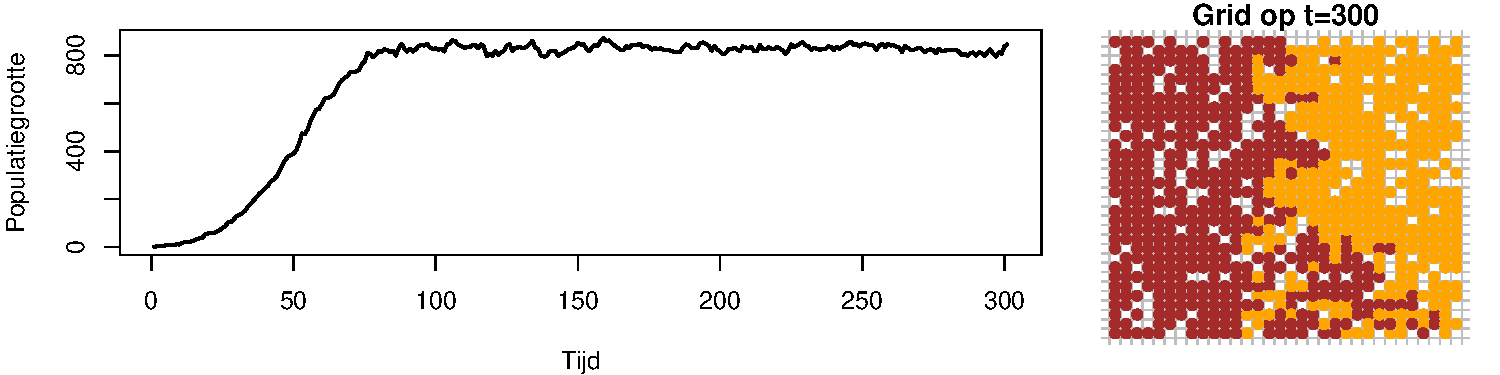
\includegraphics{Modellering/groei_ruimte_files/figure-pdf/fig-stochasticity-1.pdf}

}

}

\subcaption{\label{fig-stochasticity-1}Simulatie met b=0.6, d=0.1}
\end{minipage}%
\newline
\begin{minipage}[t]{\linewidth}

{\centering 

\raisebox{-\height}{

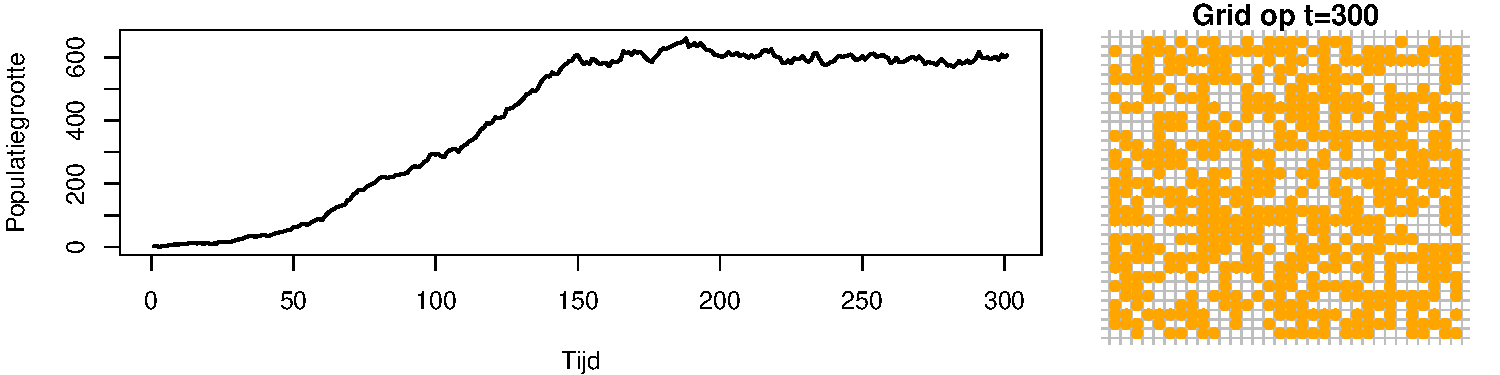
\includegraphics{Modellering/groei_ruimte_files/figure-pdf/fig-stochasticity-2.pdf}

}

}

\subcaption{\label{fig-stochasticity-2}Simulatie met b=0.3, d=0.1}
\end{minipage}%
\newline
\begin{minipage}[t]{\linewidth}

{\centering 

\raisebox{-\height}{

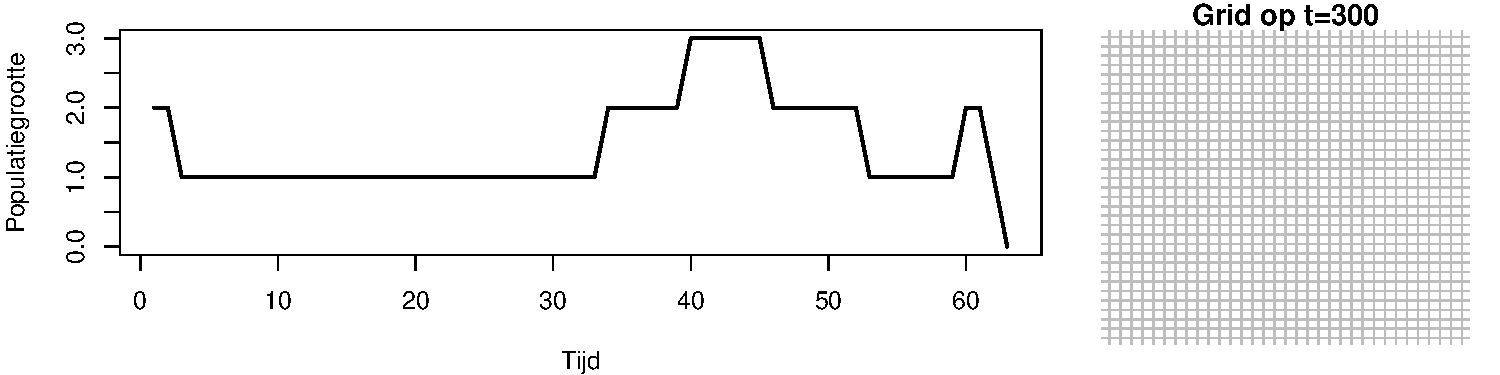
\includegraphics{Modellering/groei_ruimte_files/figure-pdf/fig-stochasticity-3.pdf}

}

}

\subcaption{\label{fig-stochasticity-3}Simulatie met b=0.12, d=0.1}
\end{minipage}%

\caption{\label{fig-stochasticity}De simulatie wanneer birth veel
waarschijnlijker is dan death.}

\end{figure}

\hypertarget{lokale-interacties-en-samenwerken}{%
\section{Lokale interacties en
samenwerken}\label{lokale-interacties-en-samenwerken}}

In de biologie is vaak sprake van samenwerking (ook wel coöperatie
genoemd). Wolven jagen samen, planten zenden chemische signalen uit om
anderen te waarschuwen voor herbivoren, en bacteriën scheiden enzymen
uit die suikers beschikbaar maken voor nabijgelegen bacteriën.
Dergelijke samenwerkingen zouden we kunnen verwerken in onze simulatie
in een vorm van dichtheidsafhankelijkheid.

Als we positieve dichtheidsafhankelijke effecten willen gebruiken in een
IBM op een grid, zouden we de totaalpopulatie kunnen meten en de kans op
geboorte (\(b\)) hiermee aan kunnen aanpassen. Echter hoeft het helemaal
niet zo te zijn dat iedereen de vruchten plukt van samenwerkingen. Als
een individu in grid-punt \texttt{(10,10)} anderen helpt (bijvoorbeeld
de bacterie maakt suikers vrij), zal een individu in gridpunt
\texttt{(25,20)} daar geen direct voordeel van hebben. In plaats
daarvan, zouden we bijvoorbeeld de geboortekans van de 8 buren van
\texttt{(10,10)} kunnen verhogen. Dit noemen we een \textbf{lokale
interactie}. Bijvoorbeeld, de oranje en rode individuen kunnen de
volgende geboortekansen krijgen:

\[ \text{Geboortekans(\color{red}rood\color{black})} = b+c\cdot (\sum{\text{aantal \color{orange}oranje \color{black} buren}})\]
\[\text{Geboortekans(\color{orange}oranje\color{black})} = b+c\cdot (\sum{\text{aantal \color{red} rode \color{black} buren}})\]

Hieronder zie je een interactieve simulatie van dit systeem (je moet nog
wel even op start drukken), waarbij je de parameters \(b\), \(c\), en
\(d\), en de begin-dichtheid kan instellen. De parameters zijn zo
ingesteld dat \(b\) maar een klein beetje groter is dan \(d\), maar
doordat de individuen elkaar helpen groeien ze toch prima uit totdat het
hele grid vol is.

WEBSHOT IS EEN LEUK IDEE, MAAR BETER MAKEN WE PRINT SCREENS MET EEN LINK
ZODAT HET IIG DE JUISTE VISUALISATIE IS\ldots{}

\begin{figure}

{\centering 

\href{https://tbb.bio.uu.nl/bvd/simulations/samenwerken/}{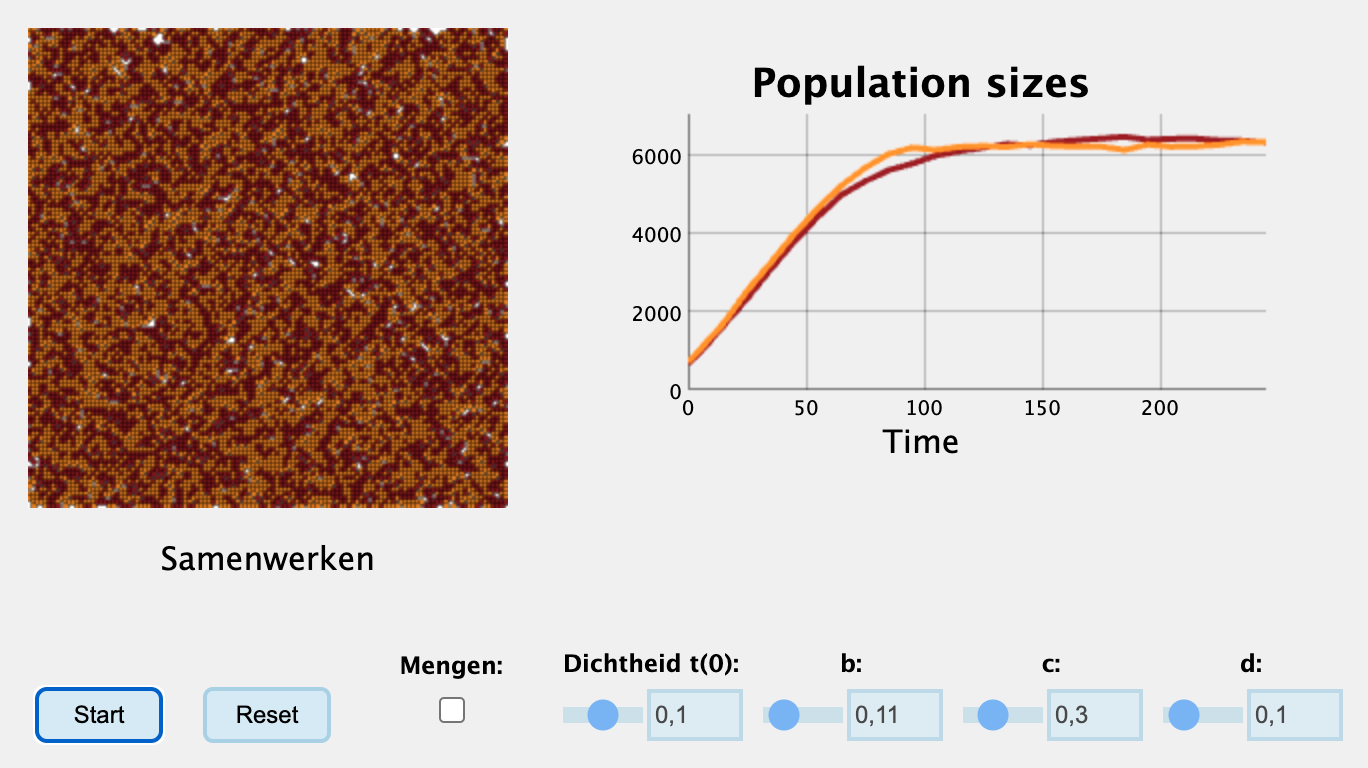
\includegraphics{Modellering/figuren/sim_samenwerken.png}}

}

\end{figure}

\url{https://tbb.bio.uu.nl/bvd/bms/simulations/samenwerken/}

Wat opvalt aan de bovenstaande simulatie is dat de populatie uitgroeit,
maar dat als we naar de grafiek kijken, dit niet exponentieel lijkt te
beginnen (met andere woorden, we zien geen sigmoïde curve). Dit zou
kunnen komen doordat we met een vrij hoge dichtheid van cellen beginnen,
waardoor we onmiddellijk al in het steile deel van de groeicurve zitten.
In het werkcollege zul je deze simulatie verder bestuderen.

\hypertarget{de-parasiet}{%
\section{De parasiet}\label{de-parasiet}}

Als we het hebben over samenwerking, kunnen we ons afvragen wat er zou
gebeuren als iemand valsspeelt. Daarom gaan we de bovenstaande
simulaties uitbreiden met een derde soort: een {parasiet}. In het Engels
worden samenwerkers vaak \emph{cooperators} worden genoemd, en heten de
parasieten vaak \emph{cheaters} of \emph{defectors}. We nemen aan dat
deze cheater geen hulp geeft, en wel wordt geholpen door zowel de rode
als oranje individuen:

\[ \text{Geboortekans(\color{red}rood\color{black})} = b+c\cdot (\sum{\text{aantal \color{orange}oranje \color{black} buren}})\]
\[\text{Geboortekans(\color{orange}oranje\color{black})} = b+c\cdot (\sum{\text{aantal \color{red} rode \color{black} buren}})\]
\[\text{Geboortekans(\color{blue}blauw\color{black})} = b+c\cdot (\sum{\text{aantal \color{red} rode \color{black} plus \color{orange}oranje \color{black} buren}})\]

Dit levert de volgende dynamica op:

HIER MOET WEBSHOT KOMEN

Zoals je ziet heeft deze verandering een enorme impact! Waar eerst de
simulatie niet veel meer veranderde nadat het grid was volgegroeid, zien
we nu het systeem alsmaar in beweging blijft. De cheaters overgroeien
steeds de cooperators, maar omdat ze daarna zichzelf niet helpen sterven
ze lokaal uit. Overgebleven cooperators kunnen de ``lege ruimte'' die
daardoor is ontstaan weer veroveren, waarna er weer cheaters komen,
\emph{etc.}. Zo gaat de simulatie alsmaar door. Als je echter het
systeem mengt, zul je zien dat ditzelfde niet gebeurt: de cheaters nemen
de hele simulatie over en alles sterft uit. Nadat alles is uitgestorven,
is het natuurlijk \emph{game over}.

\hypertarget{de-eindeloze-mogelijkheden-van-ibms}{%
\section{De eindeloze mogelijkheden van
IBMs}\label{de-eindeloze-mogelijkheden-van-ibms}}

Nu je een klein beetje een beeld hebt gekregen van individual-based
modelling, kun je je misschien voorstellen dat de mogelijkheden
eindeloos zijn. Hokjes kunnen namelijk niet alleen individuen bevatten,
maar ook voedsel, antibiotica, andere organismen, uitgescheden eiwitten,
windrichtingen en noem zo maar op. Bovendien hoeven individuen niet in
hokjes te zitten, maar zouden ze vrij door een continue ruimte kunnen
lopen, zoals de mieren in de simulatie hieronder:

Je begrijpt nu wellicht dat je met IBMs allerlei dingen simuleren:
(\emph{``the sky is the limit!''})! Maar dat is misschien niet altijd
even wenselijk. Met modellen proberen we natuurlijk (zoals in de
introductie uitgelegd) de biologie enigszins te versimpelen, dus het is
de kunst om de modellen niet te complex te maken. Aan de andere kant
kunnen modellen die te simpel zijn de plank enorm misslaan. De balans
tussen een simpel en een complex model is helemaal niet eenvoudig op te
maken. Albert Einstein begreep dit ook:

``A model should be as simple as possible, but no simpler'' -- Albert
Einstein\footnote{Eigenlijk is dit helemaal niet een werkelijke citaat
  van Einstein, maar wel de boodschap achter een vrij complex relaas
  over \emph{irreducible basic elements} en \emph{adequate
  representations}, wat toch iets minder catchy bleek te zijn.}

\hypertarget{opgaven-3}{%
\section{Opgaven}\label{opgaven-3}}

\begin{exercise}[Samenwerken en het Allee
effect]\protect\hypertarget{exr-samenwerkenallee}{}\label{exr-samenwerkenallee}

We bestuderen in deze opgave de simulatie van samenwerkende individuen
nog wat verder.

Zoals je kunt zien, laat deze populatie geen duidelijk logistische groei
zien (er is geen duidelijke S-curve). Wellicht komt dit doordat we met
een te hoge initiële dichtheid zijn begonnen.

\begin{enumerate}
\def\labelenumi{\alph{enumi}.}
\tightlist
\item
  Pas de begindichtheid aan zodat de beginpopulaties kleiner zijn. Laat
  de andere parameters op hun standaard waarde staan (\(b=0.11\),
  \(d=0.10\), en \(c=0.3\)). Herstart de simulatie een aantal keer. Wat
  valt je op bij hele lage begin-dichtheden (\(<0.002\))? \emph{de
  populaties kunnen uitsterven omdat ze elkaar niet weten te vinden}
\item
  Gebruik een begin-dichtheid van \(0.002\), en herhaal je experiment 20
  keer. Houd voor iedere keer bij of het de populatie lukt om uit te
  groeien (ja/nee). \emph{ongeveer 5/20 lukte het bij mij.. zit veel
  ruis op dit signaal}
\item
  Activeer ``mengen'', en herhaal je experiment uit \textbf{b} nogmaals
  20 keer. Houd wederom bij of de populatie succesvol kan uitgroeien
  \emph{een stuk vaker lukt dat nu}
\item
  Heb je een verschil gevonden? Zou dit verschil misschien toeval kunnen
  zijn? Bewaar al je resultaten in een tabel om deze later in het
  onderdeel ``Statistiek'' verder te analyseren. \emph{ja er is een
  verschil, en ook is de sigmoide veel steiler. of het verschil
  betrouwbaar is dat weten we nog niet, gaan we later naar kijken}
\end{enumerate}

\end{exercise}

\begin{exercise}[De simpelste ODE met
coöperatie]\protect\hypertarget{exr-desimpelstecoop}{}\label{exr-desimpelstecoop}

In een eerder hoofdstuk hebben we geleerd dat we in ODEs de birth- of
death-rates afhankelijk kunnen maken van de dichtheid. In dit hoofdstuk
hebben we kennis gemaakt met coöperatie: groei die juist
\emph{bevorderd} wordt door een hogere dichtheid. Dit zouden we in een
simpele ODE kunnen verwerken als een een birth rate die kwadratisch
afhangt van de dichtheid:

\begin{align}
    \mathchoice{\frac{\mathrm{d}N}
{\mathrm{d}t}}{\mathrm{d}N/\mathrm{d}t}
{\mathrm{d}N/\mathrm{d}t}
{\mathrm{d}N/\mathrm{d}t} &= bN^2 - dN
\end{align}

\begin{enumerate}
\def\labelenumi{\alph{enumi}.}
\tightlist
\item
  Bereken bij welke dichtheden \(N\) er sprake is van evenwicht. \%N=0
  en N=d/b
\item
  Schets \(\mathchoice{\frac{\mathrm{d}N}
  {\mathrm{d}t}}{\mathrm{d}N/\mathrm{d}t}
  {\mathrm{d}N/\mathrm{d}t}
  {\mathrm{d}N/\mathrm{d}t}\) als een functie van \(N\). Bepaal met
  behulp van dit faseportret de stabiliteit van de evenwichten.
  \emph{N=0 is stabiel, d/b is instabiel}
\item
  Schets oplossingen voor de initiële conditie waar \(N\) klein is, en
  de initiele conditie waar \(N\) groot is. Wat valt je op?
  \emph{uitsterven of oneindig groeien, maar geen interessant evenwicht}
\item
  Waarom was het fenomeen uit vraag c.~geen probleem in het
  individual-based model? \emph{daar namen we aan dat er maar 1 individu
  in een hokje past, dus oneindige groei kan niet. als alle hokjes vol
  zitten is het vol.~}
\end{enumerate}

\end{exercise}

\begin{exercise}[Logistische groei met sexuele
reproductie]\protect\hypertarget{exr-loggroeisex}{}\label{exr-loggroeisex}

Je hebt geleerd dat logistische groei in eerste instantie exponentiëel
is, waarna het afvlakt tot een plateau. In de cooperatie-vragen heb je
gezien dat hele lage dichtheden een probleem kunnen opleveren. Ditzelfde
geldt voor sexuele reproductie: bij lage dichtheden is het moeilijk een
paringspartner te vinden. Beschouw de volgende ODE vergelijking:

\begin{align}
    \mathchoice{\frac{\mathrm{d}N}
{\mathrm{d}t}}{\mathrm{d}N/\mathrm{d}t}
{\mathrm{d}N/\mathrm{d}t}
{\mathrm{d}N/\mathrm{d}t} &= bN^c(1-\frac{N}{k}) - dN
\end{align}

Dit model lijkt erg op vergelijkingen die we al hebben gezien voor
logistische groei: \(b\) staat voor de (maximale) geboortesnelheid,
\(k\) schaalt de dichtheidsafhankelijke afname van de geboorte, en \(d\)
geeft een constante sterfte. Maar er staat ook een nieuwe parameter
(\(c\)) in de vergelijking, die staat voor het coöperatie-effect (dit
kan staan voor zowel sex als andere vormen van samenwerking). Hoe werkt
deze parameter precies? Laten we eerst aannemen dat \(c=1\). Omdat
\(N^1\) gewoon \(N\) is, blijft de ODE dan gelijk aan de groeimodellen
die we al kennen.

\begin{enumerate}
\def\labelenumi{\alph{enumi}.}
\tightlist
\item
  Schets de groeisnelheid \(\mathchoice{\frac{\mathrm{d}N}
  {\mathrm{d}t}}{\mathrm{d}N/\mathrm{d}t}
  {\mathrm{d}N/\mathrm{d}t}
  {\mathrm{d}N/\mathrm{d}t}\) als een functie van \(N\). Teken onder je
  schets een faseportret met pijltjes om aan te geven bij welke
  dichtheden de populatie kan groeien, en bij welke de populatie zal
  krimpen. \emph{Standaard parabool zoals in de eerdere faseportretten }
\end{enumerate}

Nu nemen we aan dat \(c=2\). De functie krijgt nu de vorm
\(bN^2 - \frac{bN^3}{k} - dN\), die wat lastiger schetsen is. We zouden
de ABC-formule kunnen gebruiken om de nullpunten uit te rekenen, maar we
kunnen ook een stukje R-code schrijven om de grafiek te maken, of de
grafiek plotten in Desmos (beide opties staan hieronder weergegeven).

\begin{Shaded}
\begin{Highlighting}[]
\NormalTok{b}\OtherTok{=}\FloatTok{0.2}
\NormalTok{k}\OtherTok{=}\DecValTok{10}
\NormalTok{d}\OtherTok{=}\FloatTok{0.1}
\NormalTok{c}\OtherTok{=}\DecValTok{2}

\NormalTok{func }\OtherTok{\textless{}{-}} \ControlFlowTok{function}\NormalTok{(C)\{}
 \FunctionTok{return}\NormalTok{(b}\SpecialCharTok{*}\NormalTok{C}\SpecialCharTok{\^{}}\NormalTok{c}\SpecialCharTok{*}\NormalTok{(}\DecValTok{1}\SpecialCharTok{{-}}\NormalTok{C}\SpecialCharTok{/}\NormalTok{k) }\SpecialCharTok{{-}}\NormalTok{ d}\SpecialCharTok{*}\NormalTok{C)}
\NormalTok{\}}

\FunctionTok{curve}\NormalTok{(func,}\DecValTok{0}\NormalTok{,}\DecValTok{11}\NormalTok{,}\AttributeTok{lwd=}\DecValTok{2}\NormalTok{,}\AttributeTok{ylim=}\FunctionTok{c}\NormalTok{(}\SpecialCharTok{{-}}\FloatTok{0.1}\NormalTok{,}\DecValTok{3}\NormalTok{),}
       \AttributeTok{ylab=}\StringTok{"dC/dt"}\NormalTok{,}\AttributeTok{xlab=}\StringTok{"C"}\NormalTok{,}\AttributeTok{col=}\StringTok{"blue"}\NormalTok{,}
       \AttributeTok{main=}\StringTok{"dC/dt als een functie van C"}\NormalTok{)}
\FunctionTok{abline}\NormalTok{(}\AttributeTok{h=}\DecValTok{0}\NormalTok{)}
\end{Highlighting}
\end{Shaded}

\begin{enumerate}
\def\labelenumi{\alph{enumi}.}
\setcounter{enumi}{1}
\tightlist
\item
  Neem de grafiek uit R of Desmos over op papier, en schets opnieuw een
  faseportret met pijltjes eronder. Geef met open of gesloten cirkel
  respectievelijk instabiele en stabiele evenwichten aan.
\item
  Schets in 1 figuur hoe de populatie door de tijd zal groeien voor
  verschillende begin-waarden van \(N\). Schets elke kwalitatief
  verschillende oplossing (er zijn drie mogelijkheden). \emph{krimping,
  groei naar stabiel vanaf onder de parabool, en groei naar stabiel
  vanaf heel grote N}
\end{enumerate}

\end{exercise}

::: \{\#exr-kreislauf\}

\hypertarget{het-mengen-van-een-kringloop}{%
\section{Het mengen van een
kringloop}\label{het-mengen-van-een-kringloop}}

\begin{figure}

{\centering 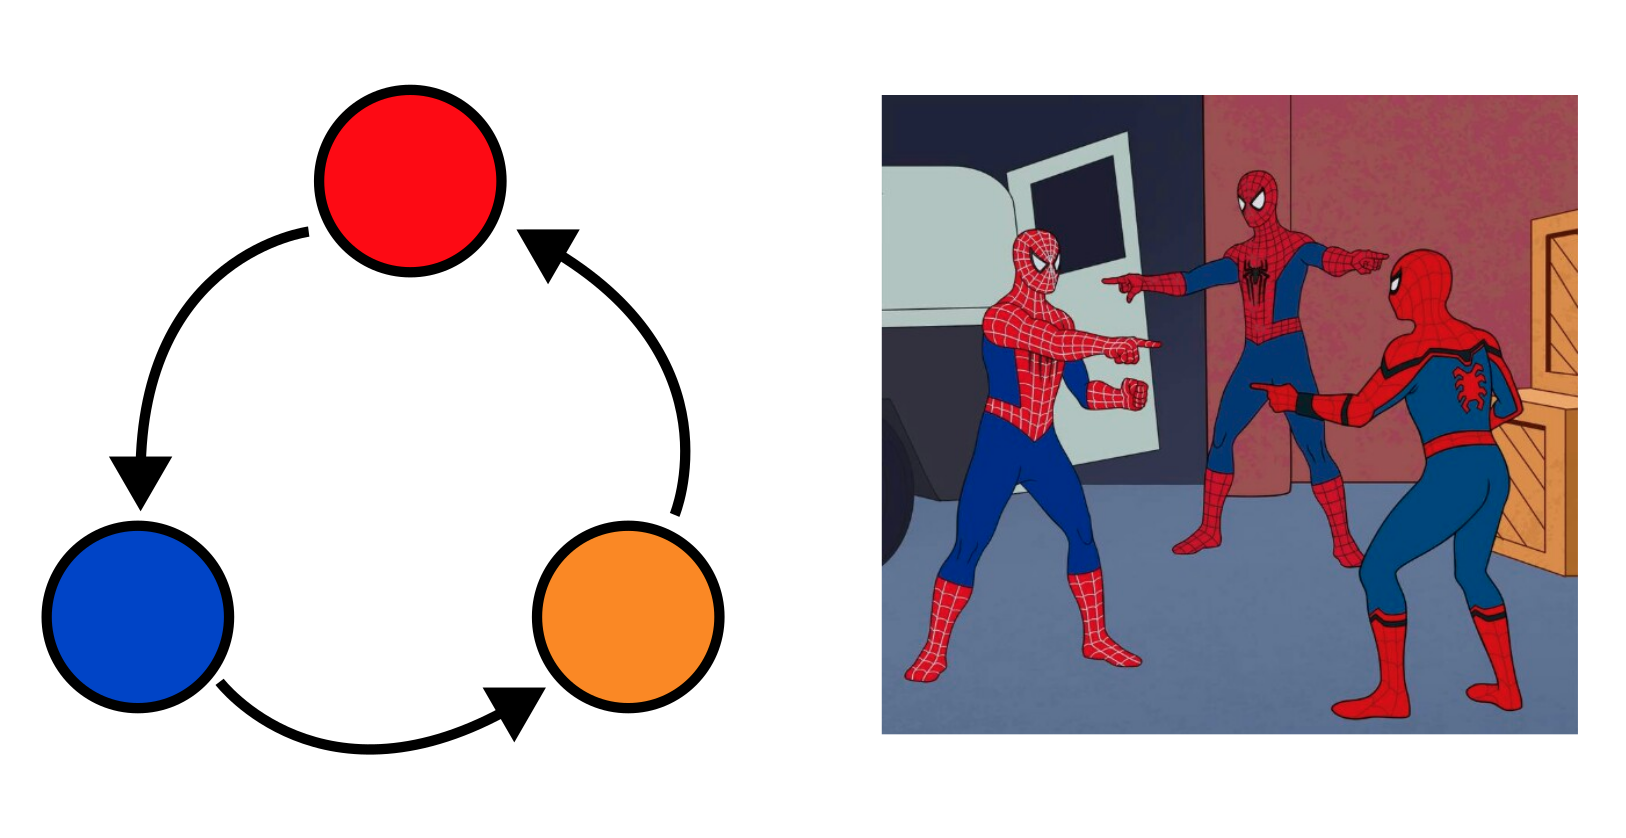
\includegraphics[width=0.8\textwidth,height=\textheight]{Modellering/figuren/kreislauf.png}

}

\caption{\emph{Gestern, heute und morgen folgen nicht aufeinander. Sie
sind in einem ewigen Kreis miteinander verbunden. Alles ist miteinander
verbunden.}}

\end{figure}

In dit hoofdstuk hebben we een voorbeeld gezien van een ``cheater'', die
wanneer het systeem goed gemengd is kan leiden tot grote problemen voor
de cooperators. Maar wat nu als de cooperators ``terug cheaten''? Wat
als er meer complexe afhankelijkheden ontstaan, zoals weergegeven in de
cyclus in bovenstaande figuur? De geboortekansen volgens deze kringloop
kunnen we definiëren als:

\begin{align}
{Geboortekans(\color{red}rood\color{black})} = b+c\cdot (\sum{\text{aantal \color{orange}oranje \color{black} buren}}) \\
{Geboortekans(\color{blue}blauw\color{black})} = b+c\cdot (\sum{\text{aantal \color{red}rode \color{black} buren}}) \\
{Geboortekans(\color{orange}oranje\color{black})} = b+c\cdot (\sum{\text{aantal \color{blue}blauwe \color{black} buren}})
\end{align}

Een simulatie met de bovenstaande interacties vind je hieronder.

\begin{enumerate}
\def\labelenumi{\alph{enumi}.}
\tightlist
\item
  Bestudeer (voor de standaardparameters \(b=0.13, c=0.11, d=0.1\)) in
  biologische begrippen op hoe dit systeem reageert op meer/minder
  mengen. Contrasteer je bevindingen met wat we gezien hebben voor het
  ``cheater-cooperator'\,' model. \emph{Door te mengen, wordt de kans om
  de juiste interatie-partners te vinden nu groter. Omdat iedereen van
  iedereen afhankeijk is, hebben we geen last van de cheater die alles
  overneemt (dat kan niet, want dan neemt de volgende op hun beurt
  over). Dit systeem heeft dus juist heel veel baad van menging.}
\end{enumerate}

In de onderstaande simulatie zijn er niet 3, maar 6 soorten die elkaar
in een vergelijkbare cyclus helpen met reproduceren.

\begin{enumerate}
\def\labelenumi{\alph{enumi}.}
\setcounter{enumi}{2}
\tightlist
\item
  Omschrijf het patroon wat er ontstaat. \emph{spirals}
\item
  Heeft mengen altijd een positieve invloed op een cyclus? \emph{niet
  helemaal. te hard mengen in dit systeem leidt tot te sterker
  fluctuaties en uitsterven}
\end{enumerate}

\hypertarget{terminologie-4}{%
\section{Terminologie}\label{terminologie-4}}

\begin{longtable}[]{@{}
  >{\raggedright\arraybackslash}p{(\columnwidth - 4\tabcolsep) * \real{0.2857}}
  >{\raggedright\arraybackslash}p{(\columnwidth - 4\tabcolsep) * \real{0.2597}}
  >{\raggedright\arraybackslash}p{(\columnwidth - 4\tabcolsep) * \real{0.4545}}@{}}
\toprule\noalign{}
\begin{minipage}[b]{\linewidth}\raggedright
Nederlands
\end{minipage} & \begin{minipage}[b]{\linewidth}\raggedright
Engels
\end{minipage} & \begin{minipage}[b]{\linewidth}\raggedright
Beschrijving
\end{minipage} \\
\midrule\noalign{}
\endhead
\bottomrule\noalign{}
\endlastfoot
Individual-based modellen & Individual-based models & Modellen waarbij
de eigenschappen en het gedrag van individuen wordt beschreven. \\
Omschrijvingsniveau & Level of description & Het belangrijkste aspect
dat een model omschrijft wordt vaak het omschrijvingsniveau genoemd.
Voor modellen van groei (bijvoorbeeld ODEs) is vaak de populatiegrootte
het omschrijvingsniveau, terwijl bij een individual-based model het
individu het omschrijvingsniveau is. \\
Modeluitkomsten & Model outcomes & Het omschrijvingsniveau bepaald sterk
welke \emph{uitkomsten} een model kan hebben: een model dat alleen
populatiegroottes omschrijft, kan geen inzichten geven in individuele
verschillen. \\
Stochasticiteit & Stochasticity & Stochastischiteit verwijst naar de
mate van willekeur of onzekerheid in een proces of in een systeem.
Zodoende zijn de uitkomsten niet volledig voorspelbaar, maar variëren
door toeval of willekeurige invloeden. In dit hoofdstuk gebruiken we
geboorte- en sterfte-kansen, waardoor bijvoorbeeld groeiende populaties
ook door domme pech uit kunnen sterven! \\
Lokale interactie & Local interaction & Interacties tussen individuen
die alleen plaatsvinden wanneer zij zich binnen een bepaalde nabije
afstand van elkaar bevinden. \\
\end{longtable}

\hypertarget{sec-meerdere}{%
\chapter{Meerdere populaties}\label{sec-meerdere}}

Biologische populaties leven nooit in isolatie, maar ondergaan
interacties met andere populaties. Neem bijvoorbeeld de populatie
konijnen in Australië, waarvoor we hebben aangenomen dat ze een
dichtheidsafhankelijke afname van hun groei hebben. Worden de
populatiegroottes van konijnen (normaal gesproken) niet ook door
predatoren beïnvloed? Is onder die omstandigheden voedselbeperking
überhaupt nog erg relevant, of gaan konijnen vooral aan predatie dood?
Om deze vragen te kunnen beantwoorden, gaan we leren om met
\textbf{systemen van differentiaalvergelijkingen} te werken.

\begin{figure}

{\centering 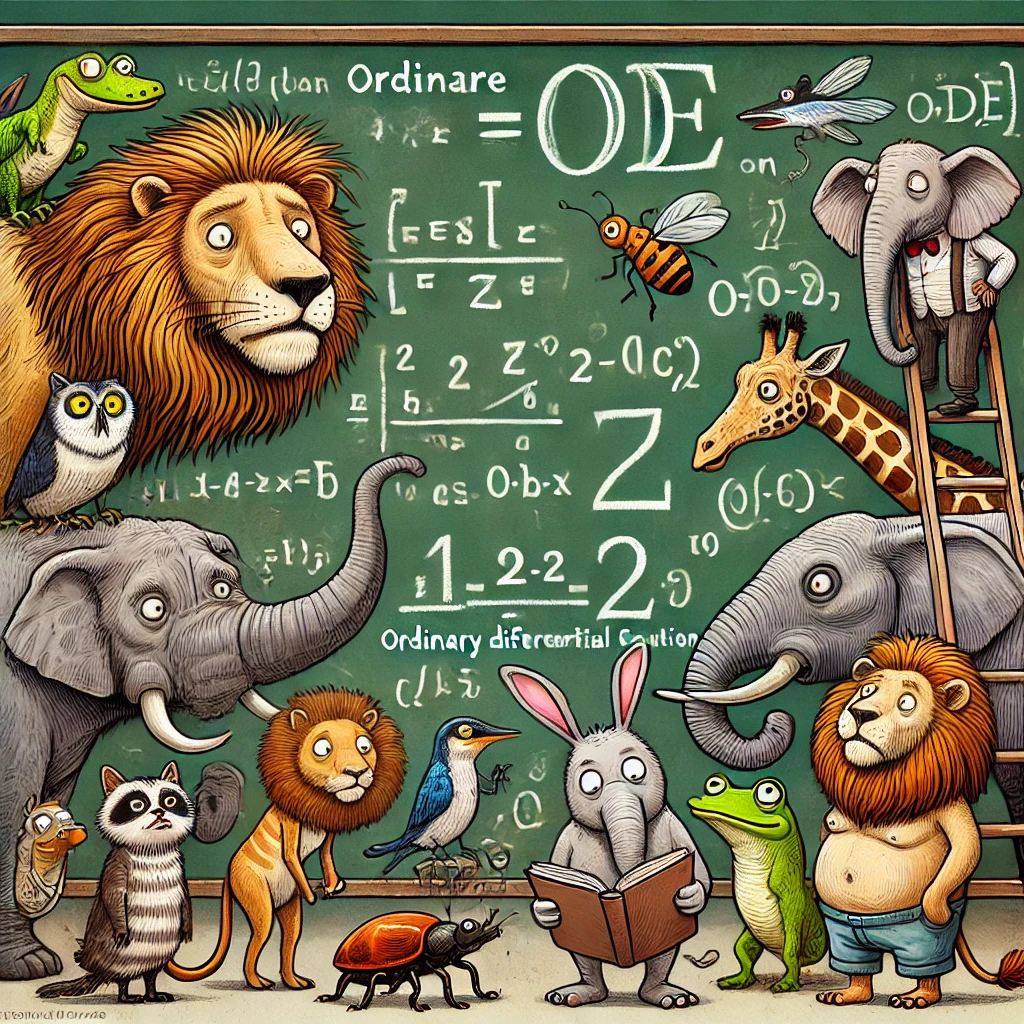
\includegraphics[width=0.8\textwidth,height=\textheight]{Modellering/figuren/meerdan1.png}

}

\caption{Afbeelding gegenereerd met ChatGPT4-o}

\end{figure}

\hypertarget{leerdoelen-5}{%
\section{Leerdoelen}\label{leerdoelen-5}}

De leerdoelen van dit onderdeel zijn:

\begin{itemize}
\tightlist
\item
  Begrijpen hoe in ODEs interacties tussen populaties worden beschreven
\item
  Beschrijven hoe een fase-ruimte in elkaar zit, en de belangrijkste
  onderdelen kunnen benoemen (nullclines, vectorveld, trajectory,
  evenwichten)
\item
  Biologische vraagstukken kunnen vertalen naar parameter-veranderingen
\item
  De consequenties van parameter-veranderingen kunnen aflezen aan een
  faseruimte
\end{itemize}

\hypertarget{konijnen-en-vossen}{%
\section{Konijnen en vossen}\label{konijnen-en-vossen}}

In het vorige hoofdstuk hebben we populaties gemodelleerd waarbij de
dichtheid de groeisnelheid verlaagt, zodat er een eindig draagvlak
ontstaat (de carrying capacity). Echter zouden we ook kunnen modelleren
dat er een dichtheidsafhankelijk effect is van een \emph{andere}
populatie. Bijvoorbeeld, als er heel veel konijnen zijn, zal een havik
of vos heel gemakkelijk een konijn te grazen nemen. Door de consumptie
van deze prooidieren, zal de predator-populatie toenemen. Laten we dit
modelleren voor konijnen en vossen, met devolgende aannames:

\begin{itemize}
\tightlist
\item
  De konijnen hebben dichtheidsafhankelijke geboorte \(b\)
\item
  De konijnen sterven met een vaste snelheid \(d\)
\item
  Predatie gebeurt met snelheid \(a\). Hoe meer konijnen en vossen, hoe
  meer predatie er zal plaatsvinden.
\item
  De groeisnelheid van vossen wordt uitsluitend bepaald door predatie
\item
  Ook vossen sterven met een vaste snelheid \(\delta\)
\end{itemize}

Deze omschrijving kunnen we ook samenvatten in \emph{functional
responses}: wiskundige functies die beschrijven hoe een populaties
reageren op hun eigen dichtheid, of die van een ander
(Figuur~\ref{fig-lvresponses}).

\begin{figure}

{\centering 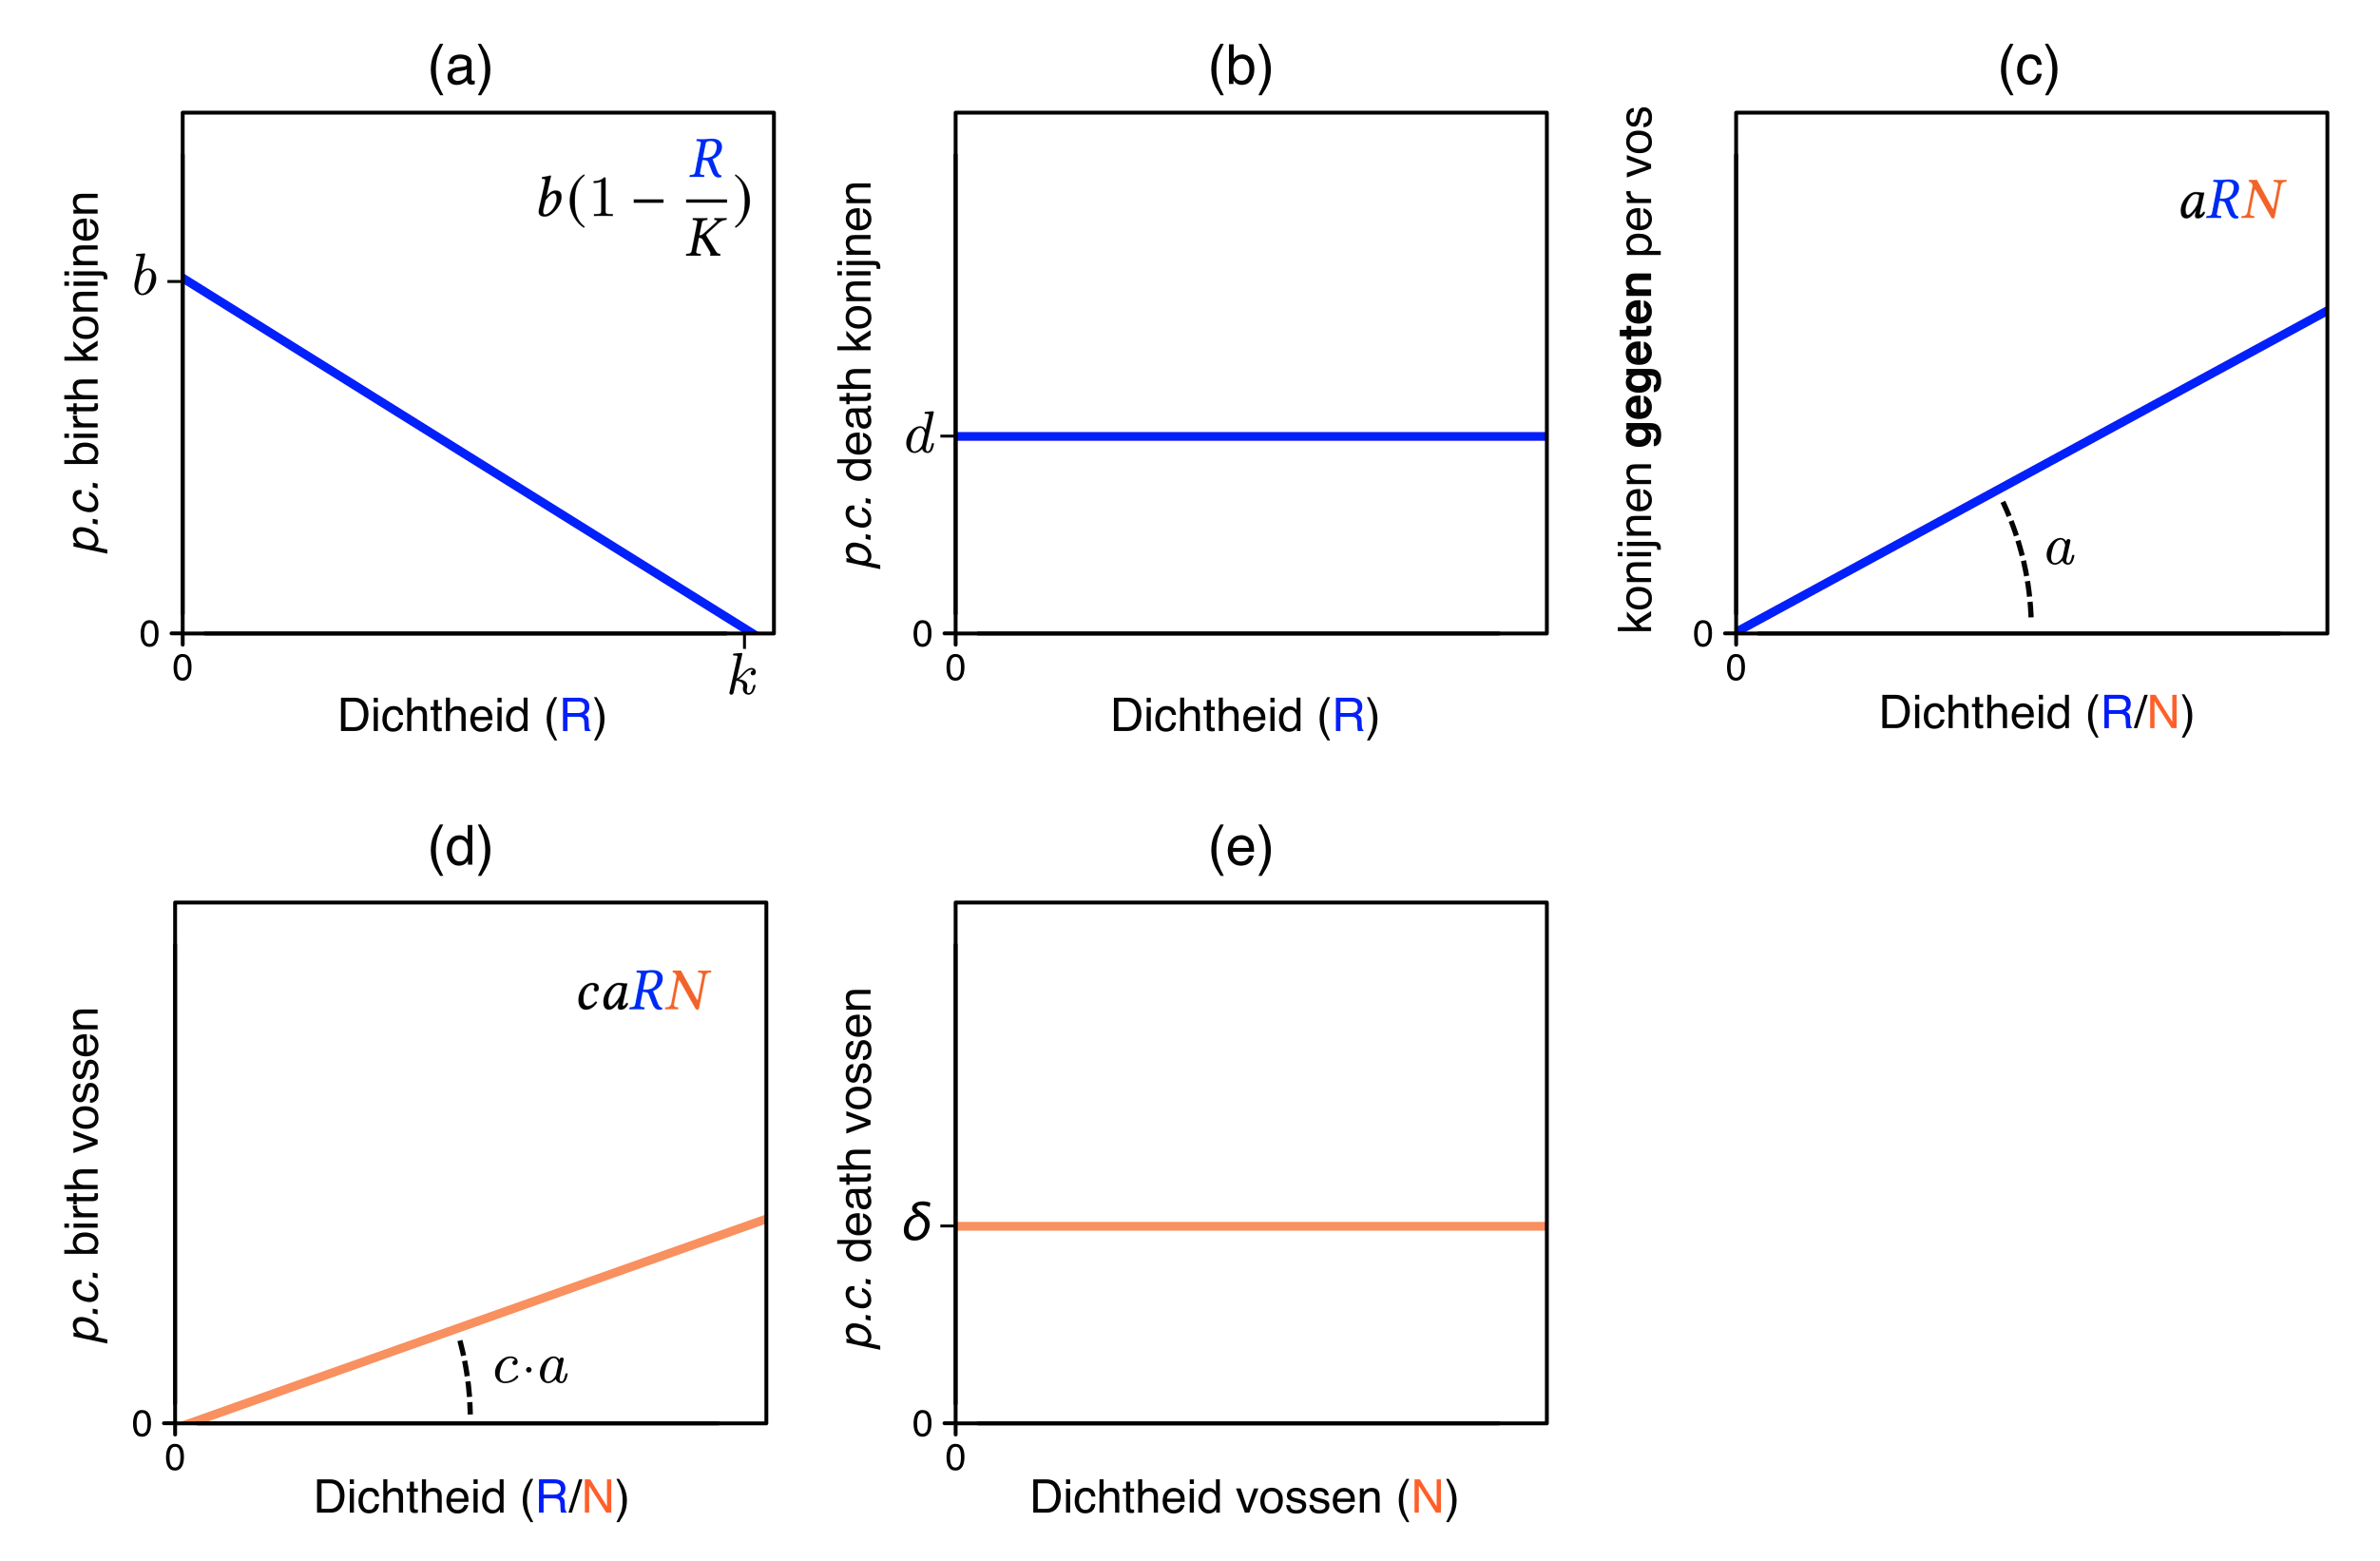
\includegraphics[width=0.8\textwidth,height=\textheight]{Modellering/figuren/LV_responses.png}

}

\caption{\label{fig-lvresponses}Afbeelding gegenereerd met ChatGPT4-o}

\end{figure}

De eerste twee processen (Figuur~\ref{fig-lvresponses} a+b, de
reproductie en sterfte van konijnen) kennen we al van het vorige
hoofdstuk. Hoewel we de konijnen eerder \(N\) hadden genoemd, is het in
dit predator-prooi model gebruikelijk om de {prooi} R te noemen. Onze
groeivergelijking voor prooidieren (met dichtheidsafhankelijke geboorte)
ziet er dan dus zo uit:

\begin{align*}
    \color{black}\frac{\mathrm{d}\color{blue}R}{\mathrm{d}t} &\color{black}= b(1-\frac{\color{blue}R}{K})\color{blue}R\color{black} - d\color{blue}R
\end{align*}

Hieraan gaan toevoegen dat vossen de konijnen opeten. De {predator} word
in deze modellen vaak aangegeven met een \(N\). We gaan ervan uit dat
predatie direct proportioneel is aan de dichtheden konijnen en vossen
(dus \(R\cdot N\)), en vermenigvuldigen dit met een nieuwe vrije
parameter (\(a \cdot R\cdot N\)) om daarmee de predatie omhoog of omlaag
te kunnen schroeven (zie Figuur~\ref{fig-lvresponses} c). Deze nieuwe
term noemen we de predatieterm. Als we de predatieterm toevoegen aan
onze vergelijking, krijgen we:

\begin{align*}
  \color{black}\frac{\mathrm{d}\color{blue}R}{\mathrm{d}t} &\color{black}= b(1-\frac{\color{blue}R}{K})\color{blue}R\color{black} - d\color{blue}R - \color{black}a\color{blue}R\color{orange}N
\end{align*}

Zoals je ziet is de variabele \(N\) anders gekleurd, om aan te geven dat
dit de {predator}-populatie is. Nu gaan we een tweede vergelijking
schrijven voor het aantal vossen. Zoals gezegd wordt hun groeisnelheid
alleen bepaald door de hoeveelheid predatie. Hiervoor kunnen we dus de
predatieterm (\(aRN\)) uit de konijnen-vergelijking hergebruiken
(Figuur~\ref{fig-lvresponses} d). Echter, omdat de biomassa van konijnen
natuurlijk niet 1-op-1 vertaalt in vossen-biomassa, kunnen we wederom
een nieuwe vrije parameter toevoegen (\(c \cdot aRN\)). Meestal nemen we
aan dat \(c<=1\), dat wil zeggen: er wordt niet meer dan 1 vos geboren
per geconsumeerd konijn. Als laatste voegen we een eenvoudig sterfteterm
toe voor de predator, en zo wordt ons uiteindelijke model:

\begin{align*}
    \color{black}\frac{\mathrm{d}\color{blue}R}{\mathrm{d}t} &\color{black}= \underbrace{b(1-\frac{\color{blue}R}{K})\color{blue}R\color{black}}_{\text{geboorte konijnen}} - 
\underbrace{d\color{blue}R}_{\text{sterfte konijnen}} - \underbrace{\color{black}a\color{blue}R\color{orange}N\color{black}}_{\text{predatie}}\\
\color{black}\frac{\mathrm{d}\color{orange}N}{\mathrm{d}t} &\color{black}= \underbrace{\color{black}ca\color{blue}R\color{orange}N\color{black}}_{\text{geboorte vossen}}\color{black} - \underbrace{\delta \color{orange}N\color{black}}_{\text{sterfte vossen}}
\end{align*}

Het bovenstaande systeem bestaat uit 2 ODEs, en wordt een 2-dimensioneel
(2D) ODE systeem genoemd. We zouden ook nog een apex predator (adelaars
bijvoorbeeld) kunnen toevoegen, en dan hebben we een 3-dimensioneel (3D)
ODE systeem (hierbij slaat 3D dus niet op ruimtelijke dimensies, maar op
de hoeveelheid variabelen van het ODE systeem). We zouden zelfs we een
heel ecosysteem kunnen opbouwen, en een 10-D of 100-D systeem
bestuderen. Voor deze ``hoogdimensionele'' systemen kunnen we vaak
alleen numeriek (met de computer) uitrekenen wat er gebeurt. Maar voor
2D systemen kunnen we nog best veel met pen-en-papier voor elkaar
krijgen.

\hypertarget{evenwichtsanalyse-van-2d-systemen}{%
\section{Evenwichtsanalyse van 2D
systemen}\label{evenwichtsanalyse-van-2d-systemen}}

In het vorige hoofdstuk hebben we geleerd dat een populatie in evenwicht
wanneer er geen verandering meer is: als de ODE gelijk is aan \(0\). Als
je werkt met meerdere ODEs, moet dit \textbf{voor elke ODE waar zijn}.
Dit is biologisch ook wel te begrijpen: de prooi is in evenwicht als
alle processen (alle termen) elkaar opheffen, maar als ondertussen de
predator nog verandert is deze balans onmiddelijk weer verstoord! We
moeten dus uitzoeken wanneer zowel de prooi-vergelijking als de
predator-vergelijking \(0\) zijn. Door de ODEs beide aan 0 gelijk te
stellen, en het stelsel met twee onbekende variabelen op te lossen,
kunnen we ontrekken waar het evenwicht precies ligt (een specifieke
hoeveelheid konijnen en vossen). Maar dit geeft eigenlijk maar weinig
inzicht in hoe de populaties veranderen over de tijd. Maar dit is nou
juist wat we graag willen weten, zodat we goed kunnen voorspellen wat er
zou kunnen gebeuren als je plotseling een wolf op de Veluwe loslaat. Hoe
gaan de populaties precies veranderen? Gaat het naar een stabiel
evenwicht? Dit kunnen we bestuderen door kennis te maken met
faseruimtes.

\hypertarget{wat-zijn-faseruimtes}{%
\section{Wat zijn faseruimtes?}\label{wat-zijn-faseruimtes}}

Omdat we te maken hebben met 2 variabelen, zijn er allerlei combinaties
mogelijk: weinig konijnen en weinig vossen, weinig konijnen en veel
vossen, veel konijnen en weinig vossen, en veel konijnen en veel vossen,
en alles daartussenin. We zouden de gehele ruimte van mogelijkheden
kunnen weergeven in een assenstelsel:

\begin{Shaded}
\begin{Highlighting}[]
\CommentTok{\#| fig.width: 7}

\CommentTok{\#| fig.height: 4}

\CommentTok{\#| code{-}fold: true}

\NormalTok{vectorfield }\OtherTok{\textless{}{-}} \ControlFlowTok{function}\NormalTok{(x,y,dx,dy)\{}

  \FunctionTok{arrows}\NormalTok{(x, y, x}\SpecialCharTok{+}\DecValTok{0}\NormalTok{, y}\SpecialCharTok{+}\NormalTok{dy, }\AttributeTok{length =} \FloatTok{0.07}\NormalTok{, }\AttributeTok{angle =} \DecValTok{20}\NormalTok{, }\AttributeTok{col=}\StringTok{"blue"}\NormalTok{,}\AttributeTok{lwd=}\DecValTok{2}\NormalTok{)}

  \FunctionTok{arrows}\NormalTok{(x, y, x}\SpecialCharTok{+}\NormalTok{dx, y}\SpecialCharTok{+}\DecValTok{0}\NormalTok{, }\AttributeTok{length =} \FloatTok{0.07}\NormalTok{, }\AttributeTok{angle =} \DecValTok{20}\NormalTok{, }\AttributeTok{col=}\StringTok{"\#f2790f"}\NormalTok{,}\AttributeTok{lwd=}\DecValTok{2}\NormalTok{)}

\NormalTok{\}}

\NormalTok{N }\OtherTok{\textless{}{-}} \DecValTok{1}\SpecialCharTok{:}\DecValTok{100}

\NormalTok{R }\OtherTok{\textless{}{-}} \DecValTok{1}\SpecialCharTok{:}\DecValTok{100}

\FunctionTok{par}\NormalTok{(}\AttributeTok{pty=}\StringTok{"s"}\NormalTok{,}\AttributeTok{mfrow=}\FunctionTok{c}\NormalTok{(}\DecValTok{1}\NormalTok{,}\DecValTok{1}\NormalTok{),}\AttributeTok{mar=}\FunctionTok{c}\NormalTok{(}\DecValTok{4}\NormalTok{,}\DecValTok{4}\NormalTok{,}\DecValTok{1}\NormalTok{,}\FloatTok{1.5}\NormalTok{))}

\FunctionTok{plot}\NormalTok{(R,N,  }\AttributeTok{col.axis=}\StringTok{"\#f2790f"}\NormalTok{,}\AttributeTok{type=}\StringTok{\textquotesingle{}n\textquotesingle{}}\NormalTok{,}\AttributeTok{xaxt=}\StringTok{\textquotesingle{}n\textquotesingle{}}\NormalTok{,}\AttributeTok{xlab=}\StringTok{""}\NormalTok{,}\AttributeTok{ylab=}\StringTok{""}\NormalTok{,}\AttributeTok{axes=}\ConstantTok{FALSE}\NormalTok{, }\AttributeTok{frame.plot=}\ConstantTok{TRUE}\NormalTok{)}

\FunctionTok{mtext}\NormalTok{(}\StringTok{"R"}\NormalTok{, }\AttributeTok{side=}\DecValTok{1}\NormalTok{, }\AttributeTok{line=}\DecValTok{2}\NormalTok{, }\AttributeTok{col=}\StringTok{"blue"}\NormalTok{, }\AttributeTok{cex=}\FloatTok{1.5}\NormalTok{, }\AttributeTok{at=}\DecValTok{90}\NormalTok{)}

\FunctionTok{mtext}\NormalTok{(}\StringTok{"N"}\NormalTok{, }\AttributeTok{side=}\DecValTok{2}\NormalTok{, }\AttributeTok{line=}\DecValTok{2}\NormalTok{, }\AttributeTok{col=}\StringTok{"\#f2790f"}\NormalTok{, }\AttributeTok{cex=}\FloatTok{1.5}\NormalTok{,}\AttributeTok{adj=}\DecValTok{1}\NormalTok{,}\AttributeTok{las=}\DecValTok{2}\NormalTok{, }\AttributeTok{at=}\DecValTok{90}\NormalTok{)}

\FunctionTok{mtext}\NormalTok{(}\StringTok{"0"}\NormalTok{, }\AttributeTok{side=}\DecValTok{2}\NormalTok{, }\AttributeTok{line=}\DecValTok{1}\NormalTok{, }\AttributeTok{col=}\StringTok{"black"}\NormalTok{, }\AttributeTok{cex=}\DecValTok{1}\NormalTok{,}\AttributeTok{adj=}\DecValTok{1}\NormalTok{,}\AttributeTok{las=}\DecValTok{2}\NormalTok{, }\AttributeTok{at=}\DecValTok{0}\NormalTok{)}

\FunctionTok{mtext}\NormalTok{(}\StringTok{"0"}\NormalTok{, }\AttributeTok{side=}\DecValTok{1}\NormalTok{, }\AttributeTok{line=}\DecValTok{1}\NormalTok{, }\AttributeTok{col=}\StringTok{"black"}\NormalTok{, }\AttributeTok{cex=}\DecValTok{1}\NormalTok{,}\AttributeTok{adj=}\DecValTok{0}\NormalTok{,}\AttributeTok{las=}\DecValTok{1}\NormalTok{, }\AttributeTok{at=}\SpecialCharTok{{-}}\DecValTok{1}\NormalTok{)}

\FunctionTok{Axis}\NormalTok{(}\AttributeTok{side=}\DecValTok{1}\NormalTok{, }\AttributeTok{labels=}\ConstantTok{FALSE}\NormalTok{)}

\FunctionTok{Axis}\NormalTok{(}\AttributeTok{side=}\DecValTok{2}\NormalTok{, }\AttributeTok{labels=}\ConstantTok{FALSE}\NormalTok{)}
\end{Highlighting}
\end{Shaded}

\begin{figure}[H]

{\centering 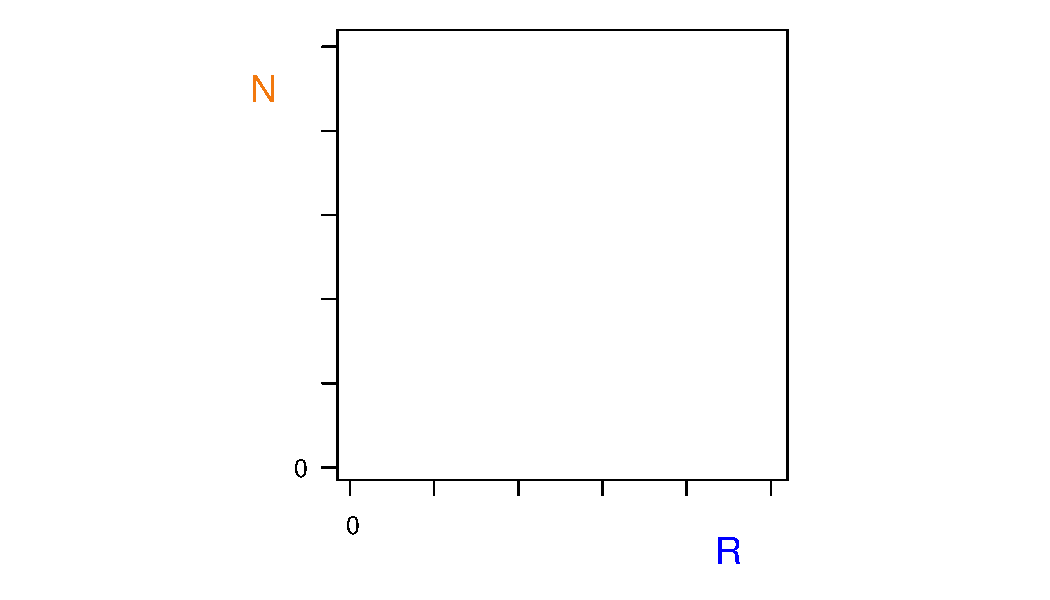
\includegraphics{Modellering/ecoevo_meerdere_files/figure-pdf/unnamed-chunk-1-1.pdf}

}

\end{figure}

\begin{Shaded}
\begin{Highlighting}[]
\CommentTok{\#vectorfield(6,10,10,{-}10)}
\end{Highlighting}
\end{Shaded}

Als we nu naar onze vergelijkingen kijken, kunnen we voor extreme
waarden van R en N proberen te beredeneren wat er gebeurt. Laten we
bijvoorbeeld kijken wat er gebeurt als er heel weinig prooien en
predatoren zijn (bijvoorbeeld 0.001 van allebei). Als we de geboorteterm
van prooien \(b(1- \frac{bR}{K})R\) uitvermenigvuldigen krijgen we
\(bR - \frac{bR^2}{K}\), en omdat we aannemen dat \(R=0.001\), is de
tweede term extra klein (want \(0.001^2 = 10^{-6}\)). Deze tweede term
is onder deze omstandigheden dus negeerbaar. Biologisch gesproken kunnen
we zeggen dat wanneer er weinig konijnen zijn, dan is
dichtheidsafhankelijke afname van groei negeerbaar. Ditzelfde principe
kunnen we toepassen op de predatieterm (\(aRN\)), waar de kleine \(R\)
en kleine \(N\) met elkaar vermenigvuldigd worden, dus dat wordt ook een
extra klein getal. Samengevat geeft dit geeft dus hetvolgende inzicht:

\begin{align*}
  \frac{\mathrm{d}\color{blue}R}{\mathrm{d}t} &=\underbrace{b\color{blue}R}_{\text{klein}} -
    \underbrace{b\color{blue}R\color{black}^2}_{\text{negeerbaar klein}} -
   \underbrace{d\color{blue}R}_{\text{klein}} - \underbrace{\color{black}a\color{blue}R\color{orange}N\color{black}}_{\text{negeerbaar klein}}
\end{align*}

Dus, als zowel \(R\) als \(N\) heel klein zijn, brengt dit onze
konijnenvergelijking terug tot:

\begin{align*}
   \frac{\mathrm{d}\color{blue}R}{\mathrm{d}t} &= b\color{blue}R\color{black} -
   d\color{blue}R
\end{align*}

Aangenomen dat \(b>d\), kan de konijnenpopulatie dus groeien.

Als we in de predator-vergelijking kijken wat er gebeurt bij hele kleine
populatiegroottes, zien we dit:

\begin{align*}
\frac{\mathrm{d}\color{orange}N}{\mathrm{d}t} &=
    \underbrace{a\color{blue}R\color{orange}N\color{black}}_{\text{negeerbaar klein}} -
    \underbrace{d\color{orange}N\color{black}}_{\text{klein}}
\end{align*}

Waardoor voor de predatoren het bij kleine dichtheden de vergelijking
teruggebracht wordt tot:

\begin{align*}
\frac{\mathrm{d}\color{orange}N\color{black}}{\mathrm{d}t} &= -d\color{orange}N
\end{align*}

Voor de predator is er bij kleine dichtheden dus alleen sterfte over.
Dit is ook wel logisch, want er is dus helemaal geen prooi aanwezig om
op te kunnen eten. De predatorpopulatie zal in deze omstandigheid dus
afnemen. Om onze inzichten samen te vatten, kunnen we linksonderin (voor
lage dichtheden van beide populaties) twee pijltjes in onze faseruimte:

\begin{Shaded}
\begin{Highlighting}[]
\CommentTok{\#| fig.width: 7}

\CommentTok{\#| fig.height: 4}

\CommentTok{\#| code{-}fold: true}

\NormalTok{vectorfield }\OtherTok{\textless{}{-}} \ControlFlowTok{function}\NormalTok{(x,y,dx,dy)\{}

  \FunctionTok{arrows}\NormalTok{(x, y, x}\SpecialCharTok{+}\DecValTok{0}\NormalTok{, y}\SpecialCharTok{+}\NormalTok{dy, }\AttributeTok{length =} \FloatTok{0.07}\NormalTok{, }\AttributeTok{angle =} \DecValTok{20}\NormalTok{, }\AttributeTok{col=}\StringTok{"\#f2790f"}\NormalTok{,}\AttributeTok{lwd=}\DecValTok{2}\NormalTok{)}

  \FunctionTok{arrows}\NormalTok{(x, y, x}\SpecialCharTok{+}\NormalTok{dx, y}\SpecialCharTok{+}\DecValTok{0}\NormalTok{, }\AttributeTok{length =} \FloatTok{0.07}\NormalTok{, }\AttributeTok{angle =} \DecValTok{20}\NormalTok{, }\AttributeTok{col=}\StringTok{"blue"}\NormalTok{,}\AttributeTok{lwd=}\DecValTok{2}\NormalTok{)}

\NormalTok{\}}

\NormalTok{N }\OtherTok{\textless{}{-}} \DecValTok{1}\SpecialCharTok{:}\DecValTok{100}

\NormalTok{R }\OtherTok{\textless{}{-}} \DecValTok{1}\SpecialCharTok{:}\DecValTok{100}

\FunctionTok{par}\NormalTok{(}\AttributeTok{pty=}\StringTok{"s"}\NormalTok{,}\AttributeTok{mfrow=}\FunctionTok{c}\NormalTok{(}\DecValTok{1}\NormalTok{,}\DecValTok{1}\NormalTok{),}\AttributeTok{mar=}\FunctionTok{c}\NormalTok{(}\DecValTok{4}\NormalTok{,}\DecValTok{4}\NormalTok{,}\DecValTok{1}\NormalTok{,}\FloatTok{1.5}\NormalTok{))}

\FunctionTok{plot}\NormalTok{(R,N,  }\AttributeTok{col.axis=}\StringTok{"\#f2790f"}\NormalTok{,}\AttributeTok{type=}\StringTok{\textquotesingle{}n\textquotesingle{}}\NormalTok{,}\AttributeTok{xaxt=}\StringTok{\textquotesingle{}n\textquotesingle{}}\NormalTok{,}\AttributeTok{xlab=}\StringTok{""}\NormalTok{,}\AttributeTok{ylab=}\StringTok{""}\NormalTok{,}\AttributeTok{axes=}\ConstantTok{FALSE}\NormalTok{, }\AttributeTok{frame.plot=}\ConstantTok{TRUE}\NormalTok{)}

\FunctionTok{mtext}\NormalTok{(}\StringTok{"R"}\NormalTok{, }\AttributeTok{side=}\DecValTok{1}\NormalTok{, }\AttributeTok{line=}\DecValTok{2}\NormalTok{, }\AttributeTok{col=}\StringTok{"blue"}\NormalTok{, }\AttributeTok{cex=}\FloatTok{1.5}\NormalTok{, }\AttributeTok{at=}\DecValTok{90}\NormalTok{)}

\FunctionTok{mtext}\NormalTok{(}\StringTok{"N"}\NormalTok{, }\AttributeTok{side=}\DecValTok{2}\NormalTok{, }\AttributeTok{line=}\DecValTok{2}\NormalTok{, }\AttributeTok{col=}\StringTok{"\#f2790f"}\NormalTok{, }\AttributeTok{cex=}\FloatTok{1.5}\NormalTok{,}\AttributeTok{adj=}\DecValTok{1}\NormalTok{,}\AttributeTok{las=}\DecValTok{2}\NormalTok{, }\AttributeTok{at=}\DecValTok{90}\NormalTok{)}

\FunctionTok{mtext}\NormalTok{(}\StringTok{"0"}\NormalTok{, }\AttributeTok{side=}\DecValTok{2}\NormalTok{, }\AttributeTok{line=}\DecValTok{1}\NormalTok{, }\AttributeTok{col=}\StringTok{"black"}\NormalTok{, }\AttributeTok{cex=}\DecValTok{1}\NormalTok{,}\AttributeTok{adj=}\DecValTok{1}\NormalTok{,}\AttributeTok{las=}\DecValTok{2}\NormalTok{, }\AttributeTok{at=}\DecValTok{0}\NormalTok{)}

\FunctionTok{mtext}\NormalTok{(}\StringTok{"0"}\NormalTok{, }\AttributeTok{side=}\DecValTok{1}\NormalTok{, }\AttributeTok{line=}\DecValTok{1}\NormalTok{, }\AttributeTok{col=}\StringTok{"black"}\NormalTok{, }\AttributeTok{cex=}\DecValTok{1}\NormalTok{,}\AttributeTok{adj=}\DecValTok{0}\NormalTok{,}\AttributeTok{las=}\DecValTok{1}\NormalTok{, }\AttributeTok{at=}\SpecialCharTok{{-}}\DecValTok{1}\NormalTok{)}

\FunctionTok{Axis}\NormalTok{(}\AttributeTok{side=}\DecValTok{1}\NormalTok{, }\AttributeTok{labels=}\ConstantTok{FALSE}\NormalTok{)}

\FunctionTok{Axis}\NormalTok{(}\AttributeTok{side=}\DecValTok{2}\NormalTok{, }\AttributeTok{labels=}\ConstantTok{FALSE}\NormalTok{)}

\FunctionTok{vectorfield}\NormalTok{(}\DecValTok{5}\NormalTok{,}\DecValTok{10}\NormalTok{,}\DecValTok{10}\NormalTok{,}\SpecialCharTok{{-}}\DecValTok{10}\NormalTok{)}
\end{Highlighting}
\end{Shaded}

\begin{figure}[H]

{\centering 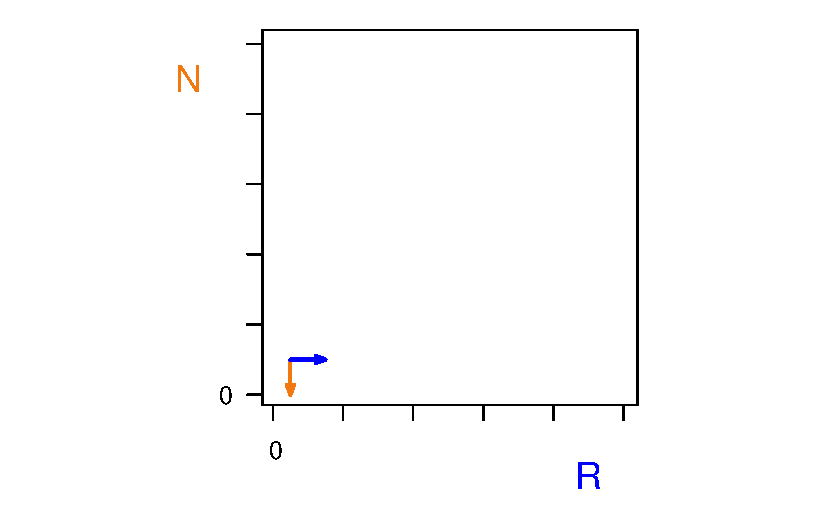
\includegraphics{Modellering/ecoevo_meerdere_files/figure-pdf/unnamed-chunk-2-1.pdf}

}

\end{figure}

Oke, dus we weten nu dat als er weinig prooi/predator is, de prooi zal
toenemen en de predator zal afnemen. Maar we weten ook dat als er meer
en meer prooi is, de prooi steeds meer negatieve dichtheidseffecten
ondervindt. De predator heeft juist alleen maar voordeel bij meer prooi.
Met andere woorden, we kunnen rechtsonderin ons diagram een pijltje
tekenen waarbij die de afname van prooi, en de toename van predatoren
weergeeft:

\begin{Shaded}
\begin{Highlighting}[]
\CommentTok{\#| fig.width: 7}

\CommentTok{\#| fig.height: 4}

\CommentTok{\#| code{-}fold: true}

\NormalTok{vectorfield }\OtherTok{\textless{}{-}} \ControlFlowTok{function}\NormalTok{(x,y,dx,dy)\{}

  \FunctionTok{arrows}\NormalTok{(x, y, x}\SpecialCharTok{+}\DecValTok{0}\NormalTok{, y}\SpecialCharTok{+}\NormalTok{dy, }\AttributeTok{length =} \FloatTok{0.07}\NormalTok{, }\AttributeTok{angle =} \DecValTok{20}\NormalTok{, }\AttributeTok{col=}\StringTok{"\#f2790f"}\NormalTok{,}\AttributeTok{lwd=}\DecValTok{2}\NormalTok{)}

  \FunctionTok{arrows}\NormalTok{(x, y, x}\SpecialCharTok{+}\NormalTok{dx, y}\SpecialCharTok{+}\DecValTok{0}\NormalTok{, }\AttributeTok{length =} \FloatTok{0.07}\NormalTok{, }\AttributeTok{angle =} \DecValTok{20}\NormalTok{, }\AttributeTok{col=}\StringTok{"blue"}\NormalTok{,}\AttributeTok{lwd=}\DecValTok{2}\NormalTok{)}

\NormalTok{\}}

\NormalTok{N }\OtherTok{\textless{}{-}} \DecValTok{1}\SpecialCharTok{:}\DecValTok{100}

\NormalTok{R }\OtherTok{\textless{}{-}} \DecValTok{1}\SpecialCharTok{:}\DecValTok{100}

\FunctionTok{par}\NormalTok{(}\AttributeTok{pty=}\StringTok{"s"}\NormalTok{,}\AttributeTok{mfrow=}\FunctionTok{c}\NormalTok{(}\DecValTok{1}\NormalTok{,}\DecValTok{1}\NormalTok{),}\AttributeTok{mar=}\FunctionTok{c}\NormalTok{(}\DecValTok{4}\NormalTok{,}\DecValTok{4}\NormalTok{,}\DecValTok{1}\NormalTok{,}\FloatTok{1.5}\NormalTok{))}

\FunctionTok{plot}\NormalTok{(R,N,  }\AttributeTok{col.axis=}\StringTok{"\#f2790f"}\NormalTok{,}\AttributeTok{type=}\StringTok{\textquotesingle{}n\textquotesingle{}}\NormalTok{,}\AttributeTok{xaxt=}\StringTok{\textquotesingle{}n\textquotesingle{}}\NormalTok{,}\AttributeTok{xlab=}\StringTok{""}\NormalTok{,}\AttributeTok{ylab=}\StringTok{""}\NormalTok{,}\AttributeTok{axes=}\ConstantTok{FALSE}\NormalTok{, }\AttributeTok{frame.plot=}\ConstantTok{TRUE}\NormalTok{)}

\FunctionTok{mtext}\NormalTok{(}\StringTok{"R"}\NormalTok{, }\AttributeTok{side=}\DecValTok{1}\NormalTok{, }\AttributeTok{line=}\DecValTok{2}\NormalTok{, }\AttributeTok{col=}\StringTok{"blue"}\NormalTok{, }\AttributeTok{cex=}\FloatTok{1.5}\NormalTok{, }\AttributeTok{at=}\DecValTok{90}\NormalTok{)}

\FunctionTok{mtext}\NormalTok{(}\StringTok{"N"}\NormalTok{, }\AttributeTok{side=}\DecValTok{2}\NormalTok{, }\AttributeTok{line=}\DecValTok{2}\NormalTok{, }\AttributeTok{col=}\StringTok{"\#f2790f"}\NormalTok{, }\AttributeTok{cex=}\FloatTok{1.5}\NormalTok{,}\AttributeTok{adj=}\DecValTok{1}\NormalTok{,}\AttributeTok{las=}\DecValTok{2}\NormalTok{, }\AttributeTok{at=}\DecValTok{90}\NormalTok{)}

\FunctionTok{mtext}\NormalTok{(}\StringTok{"0"}\NormalTok{, }\AttributeTok{side=}\DecValTok{2}\NormalTok{, }\AttributeTok{line=}\DecValTok{1}\NormalTok{, }\AttributeTok{col=}\StringTok{"black"}\NormalTok{, }\AttributeTok{cex=}\DecValTok{1}\NormalTok{,}\AttributeTok{adj=}\DecValTok{1}\NormalTok{,}\AttributeTok{las=}\DecValTok{2}\NormalTok{, }\AttributeTok{at=}\DecValTok{0}\NormalTok{)}

\FunctionTok{mtext}\NormalTok{(}\StringTok{"0"}\NormalTok{, }\AttributeTok{side=}\DecValTok{1}\NormalTok{, }\AttributeTok{line=}\DecValTok{1}\NormalTok{, }\AttributeTok{col=}\StringTok{"black"}\NormalTok{, }\AttributeTok{cex=}\DecValTok{1}\NormalTok{,}\AttributeTok{adj=}\DecValTok{0}\NormalTok{,}\AttributeTok{las=}\DecValTok{1}\NormalTok{, }\AttributeTok{at=}\SpecialCharTok{{-}}\DecValTok{1}\NormalTok{)}

\FunctionTok{Axis}\NormalTok{(}\AttributeTok{side=}\DecValTok{1}\NormalTok{, }\AttributeTok{labels=}\ConstantTok{FALSE}\NormalTok{)}

\FunctionTok{Axis}\NormalTok{(}\AttributeTok{side=}\DecValTok{2}\NormalTok{, }\AttributeTok{labels=}\ConstantTok{FALSE}\NormalTok{)}

\FunctionTok{vectorfield}\NormalTok{(}\DecValTok{5}\NormalTok{,}\DecValTok{10}\NormalTok{,}\DecValTok{10}\NormalTok{,}\SpecialCharTok{{-}}\DecValTok{10}\NormalTok{)}

\FunctionTok{vectorfield}\NormalTok{(}\DecValTok{95}\NormalTok{,}\DecValTok{5}\NormalTok{,}\SpecialCharTok{{-}}\DecValTok{10}\NormalTok{,}\DecValTok{10}\NormalTok{)}
\end{Highlighting}
\end{Shaded}

\begin{figure}[H]

{\centering 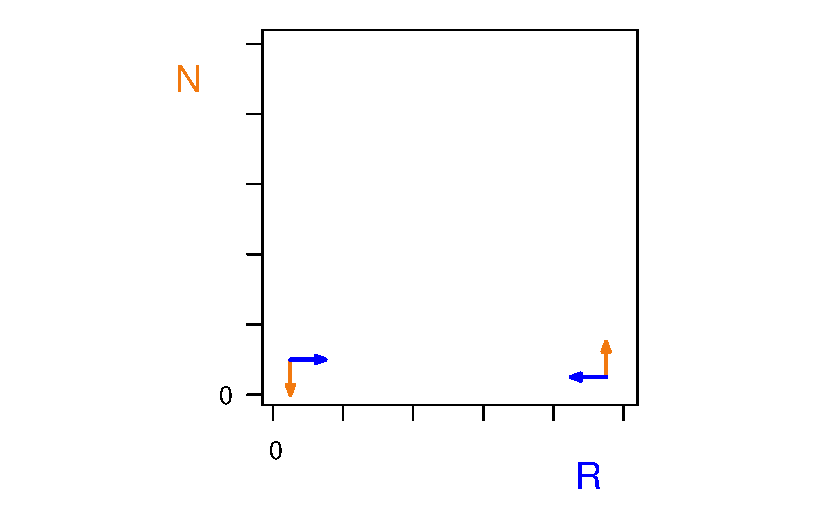
\includegraphics{Modellering/ecoevo_meerdere_files/figure-pdf/unnamed-chunk-3-1.pdf}

}

\end{figure}

\hypertarget{nullclines-en-vectorvelden}{%
\section{Nullclines en vectorvelden}\label{nullclines-en-vectorvelden}}

Uit het bovenstaande diagram kunnen we aflezen dat ergens tussen de
pijltjes links onderin en de pijltjes rechts onderin, de pijltjes van
richting zijn verandert. Neem bijvoorbeeld de groei van de predator (de
oranje pijltjes): eerst is de groei negatief, maar met genoeg prooi
wordt deze positief. Kunnen we precies bepalen \emph{waar} het oranje
pijltje is omgeklapt? Hiervoor moeten we bepalen waar in deze faseruimte
de groeisnelheid van de predator-populatie 0 is: dit geeft precies aan
waar de pijl is omgeklapt. Om dit punt te bepalen, stellen we de
predatorvergelijking gelijk aan 0:

\begin{align*}
    \color{black}ca\color{blue}R\color{orange}N\color{black} - \delta \color{orange}N &= 0\\
    \color{orange}N\color{black} \big( \color{black}ca\color{blue}R\color{black} - \delta \big) &= 0 \\
    \color{orange}N\color{black} &= 0 \qquad \text{Oplossing 1} \\
    \color{blue}R\color{black} &= \frac{\delta}{ca} \quad \text{Oplossing 2}
\end{align*}

Deze twee oplossingen, geven aan waar \(\mathchoice{\frac{\mathrm{d}N}
{\mathrm{d}t}}{\mathrm{d}N/\mathrm{d}t}
{\mathrm{d}N/\mathrm{d}t}
{\mathrm{d}N/\mathrm{d}t}\) gelijk is aan 0, en kunnen we als lijnen
tekenen in ons diagram. \(N=0\) is een horizontale lijn, en
\(R=\frac{\delta}{ca}\) een verticale lijn bij een bepaalde (positieve)
waarde van R. Waar de verticale lijn precies ligt, ligt aan de
parameters van het model. Echter weten we dat op dit punt de groei van
predatoren 0 is, dus dat hier de pijltjes omklappen. Dus: we weten dat
de verticale lijn ergens tussen onze pijltjes ligt:

\begin{Shaded}
\begin{Highlighting}[]
\CommentTok{\#| fig.width: 7}

\CommentTok{\#| fig.height: 4}

\CommentTok{\#| code{-}fold: true}

\NormalTok{vectorfield }\OtherTok{\textless{}{-}} \ControlFlowTok{function}\NormalTok{(x,y,dx,dy)\{}

  \FunctionTok{arrows}\NormalTok{(x, y, x}\SpecialCharTok{+}\DecValTok{0}\NormalTok{, y}\SpecialCharTok{+}\NormalTok{dy, }\AttributeTok{length =} \FloatTok{0.07}\NormalTok{, }\AttributeTok{angle =} \DecValTok{20}\NormalTok{, }\AttributeTok{col=}\StringTok{"\#f2790f"}\NormalTok{,}\AttributeTok{lwd=}\DecValTok{2}\NormalTok{)}

  \FunctionTok{arrows}\NormalTok{(x, y, x}\SpecialCharTok{+}\NormalTok{dx, y}\SpecialCharTok{+}\DecValTok{0}\NormalTok{, }\AttributeTok{length =} \FloatTok{0.07}\NormalTok{, }\AttributeTok{angle =} \DecValTok{20}\NormalTok{, }\AttributeTok{col=}\StringTok{"blue"}\NormalTok{,}\AttributeTok{lwd=}\DecValTok{2}\NormalTok{)}

\NormalTok{\}}

\NormalTok{N }\OtherTok{\textless{}{-}} \DecValTok{1}\SpecialCharTok{:}\DecValTok{100}

\NormalTok{R }\OtherTok{\textless{}{-}} \DecValTok{1}\SpecialCharTok{:}\DecValTok{100}

\FunctionTok{par}\NormalTok{(}\AttributeTok{pty=}\StringTok{"s"}\NormalTok{,}\AttributeTok{mfrow=}\FunctionTok{c}\NormalTok{(}\DecValTok{1}\NormalTok{,}\DecValTok{1}\NormalTok{),}\AttributeTok{mar=}\FunctionTok{c}\NormalTok{(}\DecValTok{4}\NormalTok{,}\DecValTok{4}\NormalTok{,}\DecValTok{1}\NormalTok{,}\FloatTok{1.5}\NormalTok{))}

\FunctionTok{plot}\NormalTok{(R,N,  }\AttributeTok{col.axis=}\StringTok{"\#f2790f"}\NormalTok{,}\AttributeTok{type=}\StringTok{\textquotesingle{}n\textquotesingle{}}\NormalTok{,}\AttributeTok{xaxt=}\StringTok{\textquotesingle{}n\textquotesingle{}}\NormalTok{,}\AttributeTok{xlab=}\StringTok{""}\NormalTok{,}\AttributeTok{ylab=}\StringTok{""}\NormalTok{,}\AttributeTok{axes=}\ConstantTok{FALSE}\NormalTok{, }\AttributeTok{frame.plot=}\ConstantTok{TRUE}\NormalTok{)}

\FunctionTok{mtext}\NormalTok{(}\StringTok{"R"}\NormalTok{, }\AttributeTok{side=}\DecValTok{1}\NormalTok{, }\AttributeTok{line=}\DecValTok{2}\NormalTok{, }\AttributeTok{col=}\StringTok{"blue"}\NormalTok{, }\AttributeTok{cex=}\FloatTok{1.5}\NormalTok{, }\AttributeTok{at=}\DecValTok{90}\NormalTok{)}

\FunctionTok{mtext}\NormalTok{(}\StringTok{"N"}\NormalTok{, }\AttributeTok{side=}\DecValTok{2}\NormalTok{, }\AttributeTok{line=}\DecValTok{2}\NormalTok{, }\AttributeTok{col=}\StringTok{"\#f2790f"}\NormalTok{, }\AttributeTok{cex=}\FloatTok{1.5}\NormalTok{,}\AttributeTok{adj=}\DecValTok{1}\NormalTok{,}\AttributeTok{las=}\DecValTok{2}\NormalTok{, }\AttributeTok{at=}\DecValTok{90}\NormalTok{)}

\FunctionTok{mtext}\NormalTok{(}\StringTok{"0"}\NormalTok{, }\AttributeTok{side=}\DecValTok{2}\NormalTok{, }\AttributeTok{line=}\DecValTok{1}\NormalTok{, }\AttributeTok{col=}\StringTok{"black"}\NormalTok{, }\AttributeTok{cex=}\DecValTok{1}\NormalTok{,}\AttributeTok{adj=}\DecValTok{1}\NormalTok{,}\AttributeTok{las=}\DecValTok{2}\NormalTok{, }\AttributeTok{at=}\DecValTok{0}\NormalTok{)}

\FunctionTok{mtext}\NormalTok{(}\StringTok{"0"}\NormalTok{, }\AttributeTok{side=}\DecValTok{1}\NormalTok{, }\AttributeTok{line=}\DecValTok{1}\NormalTok{, }\AttributeTok{col=}\StringTok{"black"}\NormalTok{, }\AttributeTok{cex=}\DecValTok{1}\NormalTok{,}\AttributeTok{adj=}\DecValTok{0}\NormalTok{,}\AttributeTok{las=}\DecValTok{1}\NormalTok{, }\AttributeTok{at=}\SpecialCharTok{{-}}\DecValTok{1}\NormalTok{)}

\FunctionTok{Axis}\NormalTok{(}\AttributeTok{side=}\DecValTok{1}\NormalTok{, }\AttributeTok{labels=}\ConstantTok{FALSE}\NormalTok{)}

\FunctionTok{Axis}\NormalTok{(}\AttributeTok{side=}\DecValTok{2}\NormalTok{, }\AttributeTok{labels=}\ConstantTok{FALSE}\NormalTok{)}

\FunctionTok{vectorfield}\NormalTok{(}\DecValTok{5}\NormalTok{,}\DecValTok{12}\NormalTok{,}\DecValTok{10}\NormalTok{,}\SpecialCharTok{{-}}\DecValTok{10}\NormalTok{)}

\FunctionTok{vectorfield}\NormalTok{(}\DecValTok{95}\NormalTok{,}\DecValTok{6}\NormalTok{,}\SpecialCharTok{{-}}\DecValTok{10}\NormalTok{,}\DecValTok{10}\NormalTok{)}

 \FunctionTok{abline}\NormalTok{(}\AttributeTok{h=}\DecValTok{0}\NormalTok{, }\AttributeTok{lwd=}\DecValTok{2}\NormalTok{, }\AttributeTok{col=}\StringTok{"\#f2790f"}\NormalTok{)}

 \FunctionTok{abline}\NormalTok{(}\AttributeTok{v=}\DecValTok{40}\NormalTok{, }\AttributeTok{lwd=}\DecValTok{2}\NormalTok{, }\AttributeTok{col=}\StringTok{"\#f2790f"}\NormalTok{)}
\end{Highlighting}
\end{Shaded}

\begin{figure}[H]

{\centering 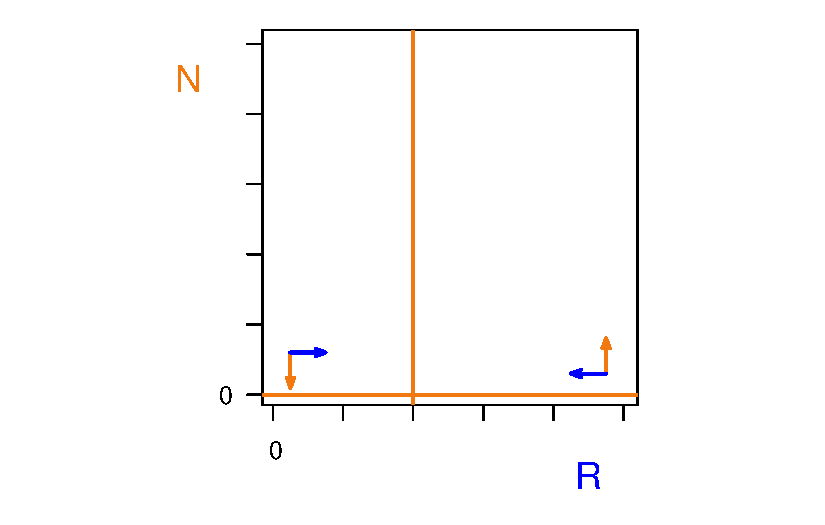
\includegraphics{Modellering/ecoevo_meerdere_files/figure-pdf/unnamed-chunk-4-1.pdf}

}

\end{figure}

De lijnen die we hierboven geschetst hebben heten null-iscoclines, of
kortgezegd: \textit{nullclines}. Een nullcline is een lijn in de
faseruimte waar de verandering van één van de variabelen (in dit geval
de groei van populaties) nul is. We kunnen ook de nullclines voor de
prooi bepalen:

\begin{align*}
    b(1-\frac{\color{blue}R}{K})\color{blue}R\color{black} - d\color{blue}R - \color{black}a\color{blue}R\color{orange}N &= 0 \\
    \color{blue}R\color{black} \big( b(1-\frac{\color{blue}R}{K})\color{black} - d - a\color{orange}N\color{black} \big) &= 0\\
    \color{blue}R &= 0 \quad \text{(oplossing 1)} \\
    b(1-\frac{\color{blue}R}{K})\color{black} - d - a\color{orange}N\color{black} &= 0 \\
    a\color{orange}N\color{black} &= b(1-\frac{\color{blue}R}{K})\color{black} - d  \\
    \color{orange}N\color{black} &= \frac{b(1-\frac{\color{blue}R}{K})\color{black} - d}{a} \quad \text{(oplossing 2)}
\end{align*}

De eerste nullcline ligt dus bij R=0 (en is dus verticaal). De tweede
nullcline ziet er wat ingewikkelder uit, want hier is \(N\) een functie
van \(R\) (met andere woorden \(N=f(R)\)). Dit is conceptueel niet heel
anders dan ``y als een functie van x'\,', zoals je misschien gewend
bent. Je ziet dat \(N\) lineair afneemt met \(R\), dus dat dit een
schuine lijn naar beneden zal vormen in ons assenstelsel. Met alle
nullclines bij elkaar, zien we dus:

\begin{Shaded}
\begin{Highlighting}[]
\CommentTok{\#| fig.width: 7}

\CommentTok{\#| fig.height: 4}

\CommentTok{\#| code{-}fold: true}

\NormalTok{vectorfield }\OtherTok{\textless{}{-}} \ControlFlowTok{function}\NormalTok{(x,y,dx,dy)\{}

  \FunctionTok{arrows}\NormalTok{(x, y, x}\SpecialCharTok{+}\DecValTok{0}\NormalTok{, y}\SpecialCharTok{+}\NormalTok{dy, }\AttributeTok{length =} \FloatTok{0.07}\NormalTok{, }\AttributeTok{angle =} \DecValTok{20}\NormalTok{, }\AttributeTok{col=}\StringTok{"\#f2790f"}\NormalTok{,}\AttributeTok{lwd=}\DecValTok{2}\NormalTok{)}

  \FunctionTok{arrows}\NormalTok{(x, y, x}\SpecialCharTok{+}\NormalTok{dx, y}\SpecialCharTok{+}\DecValTok{0}\NormalTok{, }\AttributeTok{length =} \FloatTok{0.07}\NormalTok{, }\AttributeTok{angle =} \DecValTok{20}\NormalTok{, }\AttributeTok{col=}\StringTok{"blue"}\NormalTok{,}\AttributeTok{lwd=}\DecValTok{2}\NormalTok{)}

\NormalTok{\}}

\NormalTok{N }\OtherTok{\textless{}{-}} \DecValTok{1}\SpecialCharTok{:}\DecValTok{100}

\NormalTok{R }\OtherTok{\textless{}{-}} \DecValTok{1}\SpecialCharTok{:}\DecValTok{100}

\FunctionTok{par}\NormalTok{(}\AttributeTok{pty=}\StringTok{"s"}\NormalTok{,}\AttributeTok{mfrow=}\FunctionTok{c}\NormalTok{(}\DecValTok{1}\NormalTok{,}\DecValTok{1}\NormalTok{),}\AttributeTok{mar=}\FunctionTok{c}\NormalTok{(}\DecValTok{4}\NormalTok{,}\DecValTok{4}\NormalTok{,}\DecValTok{1}\NormalTok{,}\FloatTok{1.5}\NormalTok{))}

\FunctionTok{plot}\NormalTok{(R,N,  }\AttributeTok{col.axis=}\StringTok{"\#f2790f"}\NormalTok{,}\AttributeTok{type=}\StringTok{\textquotesingle{}n\textquotesingle{}}\NormalTok{,}\AttributeTok{xaxt=}\StringTok{\textquotesingle{}n\textquotesingle{}}\NormalTok{,}\AttributeTok{xlab=}\StringTok{""}\NormalTok{,}\AttributeTok{ylab=}\StringTok{""}\NormalTok{,}\AttributeTok{axes=}\ConstantTok{FALSE}\NormalTok{, }\AttributeTok{frame.plot=}\ConstantTok{TRUE}\NormalTok{)}

\FunctionTok{mtext}\NormalTok{(}\StringTok{"R"}\NormalTok{, }\AttributeTok{side=}\DecValTok{1}\NormalTok{, }\AttributeTok{line=}\DecValTok{2}\NormalTok{, }\AttributeTok{col=}\StringTok{"blue"}\NormalTok{, }\AttributeTok{cex=}\FloatTok{1.5}\NormalTok{, }\AttributeTok{at=}\DecValTok{90}\NormalTok{)}

\FunctionTok{mtext}\NormalTok{(}\StringTok{"N"}\NormalTok{, }\AttributeTok{side=}\DecValTok{2}\NormalTok{, }\AttributeTok{line=}\DecValTok{2}\NormalTok{, }\AttributeTok{col=}\StringTok{"\#f2790f"}\NormalTok{, }\AttributeTok{cex=}\FloatTok{1.5}\NormalTok{,}\AttributeTok{adj=}\DecValTok{1}\NormalTok{,}\AttributeTok{las=}\DecValTok{2}\NormalTok{, }\AttributeTok{at=}\DecValTok{90}\NormalTok{)}

\FunctionTok{mtext}\NormalTok{(}\StringTok{"0"}\NormalTok{, }\AttributeTok{side=}\DecValTok{2}\NormalTok{, }\AttributeTok{line=}\DecValTok{1}\NormalTok{, }\AttributeTok{col=}\StringTok{"black"}\NormalTok{, }\AttributeTok{cex=}\DecValTok{1}\NormalTok{,}\AttributeTok{adj=}\DecValTok{1}\NormalTok{,}\AttributeTok{las=}\DecValTok{2}\NormalTok{, }\AttributeTok{at=}\DecValTok{0}\NormalTok{)}

\FunctionTok{mtext}\NormalTok{(}\StringTok{"0"}\NormalTok{, }\AttributeTok{side=}\DecValTok{1}\NormalTok{, }\AttributeTok{line=}\DecValTok{1}\NormalTok{, }\AttributeTok{col=}\StringTok{"black"}\NormalTok{, }\AttributeTok{cex=}\DecValTok{1}\NormalTok{,}\AttributeTok{adj=}\DecValTok{0}\NormalTok{,}\AttributeTok{las=}\DecValTok{1}\NormalTok{, }\AttributeTok{at=}\SpecialCharTok{{-}}\DecValTok{1}\NormalTok{)}

\FunctionTok{Axis}\NormalTok{(}\AttributeTok{side=}\DecValTok{1}\NormalTok{, }\AttributeTok{labels=}\ConstantTok{FALSE}\NormalTok{)}

\FunctionTok{Axis}\NormalTok{(}\AttributeTok{side=}\DecValTok{2}\NormalTok{, }\AttributeTok{labels=}\ConstantTok{FALSE}\NormalTok{)}

\FunctionTok{vectorfield}\NormalTok{(}\DecValTok{5}\NormalTok{,}\DecValTok{12}\NormalTok{,}\DecValTok{10}\NormalTok{,}\SpecialCharTok{{-}}\DecValTok{10}\NormalTok{)}

\FunctionTok{vectorfield}\NormalTok{(}\DecValTok{95}\NormalTok{,}\DecValTok{6}\NormalTok{,}\SpecialCharTok{{-}}\DecValTok{10}\NormalTok{,}\DecValTok{10}\NormalTok{)}

 \FunctionTok{abline}\NormalTok{(}\AttributeTok{h=}\DecValTok{0}\NormalTok{, }\AttributeTok{lwd=}\DecValTok{2}\NormalTok{, }\AttributeTok{col=}\StringTok{"\#f2790f"}\NormalTok{)}

 \FunctionTok{abline}\NormalTok{(}\AttributeTok{v=}\DecValTok{40}\NormalTok{, }\AttributeTok{lwd=}\DecValTok{2}\NormalTok{, }\AttributeTok{col=}\StringTok{"\#f2790f"}\NormalTok{)}

 \FunctionTok{abline}\NormalTok{(}\AttributeTok{v=}\DecValTok{0}\NormalTok{, }\AttributeTok{lwd=}\DecValTok{2}\NormalTok{, }\AttributeTok{col=}\StringTok{"blue"}\NormalTok{,)}

 \FunctionTok{abline}\NormalTok{(}\AttributeTok{a=}\DecValTok{80}\NormalTok{,}\AttributeTok{b=}\SpecialCharTok{{-}}\DecValTok{1}\NormalTok{, }\AttributeTok{lwd=}\DecValTok{2}\NormalTok{,}\AttributeTok{col=}\StringTok{"blue"}\NormalTok{)}
\end{Highlighting}
\end{Shaded}

\begin{figure}[H]

{\centering 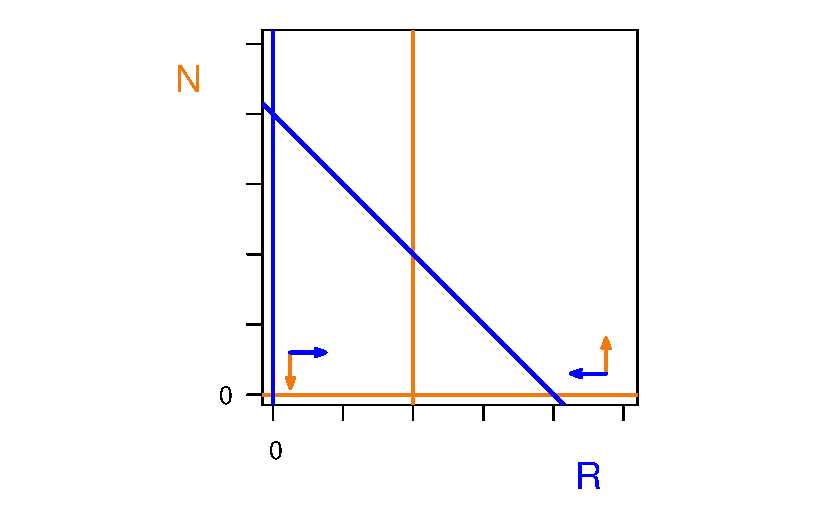
\includegraphics{Modellering/ecoevo_meerdere_files/figure-pdf/unnamed-chunk-5-1.pdf}

}

\end{figure}

De pijltjes die in ons diagram geven het zogenoemde ``vectorveld'\,'
aan. We weten dat \textbf{op} de nullclines één van de populaties niet
groeit, omdat de corresponderende differentiaalvergelijking hier gelijk
is aan 0. Vergelijkbaar is de groeisnelheid van deze populatie steeds
lager naarmate je dichter bij de nullcline kijkt. Als je de nullcline
passeert, passeer je de 0 en zal het pijltje (de richting van groei)
andersom staan. Met deze informatie kunnen we het puzzeltje oplossen, en
de andere hoeken van het vectorveld ook invullen:

\begin{Shaded}
\begin{Highlighting}[]
\CommentTok{\#| fig.width: 7}

\CommentTok{\#| fig.height: 4}

\CommentTok{\#| code{-}fold: true}

\NormalTok{vectorfield }\OtherTok{\textless{}{-}} \ControlFlowTok{function}\NormalTok{(x,y,dx,dy)\{}

  \FunctionTok{arrows}\NormalTok{(x, y, x}\SpecialCharTok{+}\DecValTok{0}\NormalTok{, y}\SpecialCharTok{+}\NormalTok{dy, }\AttributeTok{length =} \FloatTok{0.07}\NormalTok{, }\AttributeTok{angle =} \DecValTok{20}\NormalTok{, }\AttributeTok{col=}\StringTok{"\#f2790f"}\NormalTok{,}\AttributeTok{lwd=}\DecValTok{2}\NormalTok{)}

  \FunctionTok{arrows}\NormalTok{(x, y, x}\SpecialCharTok{+}\NormalTok{dx, y}\SpecialCharTok{+}\DecValTok{0}\NormalTok{, }\AttributeTok{length =} \FloatTok{0.07}\NormalTok{, }\AttributeTok{angle =} \DecValTok{20}\NormalTok{, }\AttributeTok{col=}\StringTok{"blue"}\NormalTok{,}\AttributeTok{lwd=}\DecValTok{2}\NormalTok{)}

\NormalTok{\}}

\NormalTok{N }\OtherTok{\textless{}{-}} \DecValTok{1}\SpecialCharTok{:}\DecValTok{100}

\NormalTok{R }\OtherTok{\textless{}{-}} \DecValTok{1}\SpecialCharTok{:}\DecValTok{100}

\FunctionTok{par}\NormalTok{(}\AttributeTok{pty=}\StringTok{"s"}\NormalTok{,}\AttributeTok{mfrow=}\FunctionTok{c}\NormalTok{(}\DecValTok{1}\NormalTok{,}\DecValTok{1}\NormalTok{),}\AttributeTok{mar=}\FunctionTok{c}\NormalTok{(}\DecValTok{4}\NormalTok{,}\DecValTok{4}\NormalTok{,}\DecValTok{1}\NormalTok{,}\FloatTok{1.5}\NormalTok{))}

\FunctionTok{plot}\NormalTok{(R,N,  }\AttributeTok{col.axis=}\StringTok{"\#f2790f"}\NormalTok{,}\AttributeTok{type=}\StringTok{\textquotesingle{}n\textquotesingle{}}\NormalTok{,}\AttributeTok{xaxt=}\StringTok{\textquotesingle{}n\textquotesingle{}}\NormalTok{,}\AttributeTok{xlab=}\StringTok{""}\NormalTok{,}\AttributeTok{ylab=}\StringTok{""}\NormalTok{,}\AttributeTok{axes=}\ConstantTok{FALSE}\NormalTok{, }\AttributeTok{frame.plot=}\ConstantTok{TRUE}\NormalTok{)}

\FunctionTok{mtext}\NormalTok{(}\StringTok{"R"}\NormalTok{, }\AttributeTok{side=}\DecValTok{1}\NormalTok{, }\AttributeTok{line=}\DecValTok{2}\NormalTok{, }\AttributeTok{col=}\StringTok{"blue"}\NormalTok{, }\AttributeTok{cex=}\FloatTok{1.5}\NormalTok{, }\AttributeTok{at=}\DecValTok{90}\NormalTok{)}

\FunctionTok{mtext}\NormalTok{(}\StringTok{"N"}\NormalTok{, }\AttributeTok{side=}\DecValTok{2}\NormalTok{, }\AttributeTok{line=}\DecValTok{2}\NormalTok{, }\AttributeTok{col=}\StringTok{"\#f2790f"}\NormalTok{, }\AttributeTok{cex=}\FloatTok{1.5}\NormalTok{,}\AttributeTok{adj=}\DecValTok{1}\NormalTok{,}\AttributeTok{las=}\DecValTok{2}\NormalTok{, }\AttributeTok{at=}\DecValTok{90}\NormalTok{)}

\FunctionTok{mtext}\NormalTok{(}\StringTok{"0"}\NormalTok{, }\AttributeTok{side=}\DecValTok{2}\NormalTok{, }\AttributeTok{line=}\DecValTok{1}\NormalTok{, }\AttributeTok{col=}\StringTok{"black"}\NormalTok{, }\AttributeTok{cex=}\DecValTok{1}\NormalTok{,}\AttributeTok{adj=}\DecValTok{1}\NormalTok{,}\AttributeTok{las=}\DecValTok{2}\NormalTok{, }\AttributeTok{at=}\DecValTok{0}\NormalTok{)}

\FunctionTok{mtext}\NormalTok{(}\StringTok{"0"}\NormalTok{, }\AttributeTok{side=}\DecValTok{1}\NormalTok{, }\AttributeTok{line=}\DecValTok{1}\NormalTok{, }\AttributeTok{col=}\StringTok{"black"}\NormalTok{, }\AttributeTok{cex=}\DecValTok{1}\NormalTok{,}\AttributeTok{adj=}\DecValTok{0}\NormalTok{,}\AttributeTok{las=}\DecValTok{1}\NormalTok{, }\AttributeTok{at=}\SpecialCharTok{{-}}\DecValTok{1}\NormalTok{)}

\FunctionTok{Axis}\NormalTok{(}\AttributeTok{side=}\DecValTok{1}\NormalTok{, }\AttributeTok{labels=}\ConstantTok{FALSE}\NormalTok{)}

\FunctionTok{Axis}\NormalTok{(}\AttributeTok{side=}\DecValTok{2}\NormalTok{, }\AttributeTok{labels=}\ConstantTok{FALSE}\NormalTok{)}

\FunctionTok{vectorfield}\NormalTok{(}\DecValTok{5}\NormalTok{,}\DecValTok{12}\NormalTok{,}\DecValTok{10}\NormalTok{,}\SpecialCharTok{{-}}\DecValTok{10}\NormalTok{)}

\FunctionTok{vectorfield}\NormalTok{(}\DecValTok{95}\NormalTok{,}\DecValTok{6}\NormalTok{,}\SpecialCharTok{{-}}\DecValTok{10}\NormalTok{,}\DecValTok{10}\NormalTok{)}

\FunctionTok{vectorfield}\NormalTok{(}\DecValTok{50}\NormalTok{,}\DecValTok{6}\NormalTok{,}\DecValTok{10}\NormalTok{,}\DecValTok{10}\NormalTok{)}

\FunctionTok{vectorfield}\NormalTok{(}\DecValTok{15}\NormalTok{,}\DecValTok{95}\NormalTok{,}\SpecialCharTok{{-}}\DecValTok{10}\NormalTok{,}\SpecialCharTok{{-}}\DecValTok{10}\NormalTok{)}

 \FunctionTok{abline}\NormalTok{(}\AttributeTok{h=}\DecValTok{0}\NormalTok{, }\AttributeTok{lwd=}\DecValTok{2}\NormalTok{, }\AttributeTok{col=}\StringTok{"\#f2790f"}\NormalTok{)}

 \FunctionTok{abline}\NormalTok{(}\AttributeTok{v=}\DecValTok{40}\NormalTok{, }\AttributeTok{lwd=}\DecValTok{2}\NormalTok{, }\AttributeTok{col=}\StringTok{"\#f2790f"}\NormalTok{)}

 \FunctionTok{abline}\NormalTok{(}\AttributeTok{v=}\DecValTok{0}\NormalTok{, }\AttributeTok{lwd=}\DecValTok{2}\NormalTok{, }\AttributeTok{col=}\StringTok{"blue"}\NormalTok{,)}

 \FunctionTok{abline}\NormalTok{(}\AttributeTok{a=}\DecValTok{80}\NormalTok{,}\AttributeTok{b=}\SpecialCharTok{{-}}\DecValTok{1}\NormalTok{, }\AttributeTok{lwd=}\DecValTok{2}\NormalTok{,}\AttributeTok{col=}\StringTok{"blue"}\NormalTok{)}
\end{Highlighting}
\end{Shaded}

\begin{figure}[H]

{\centering 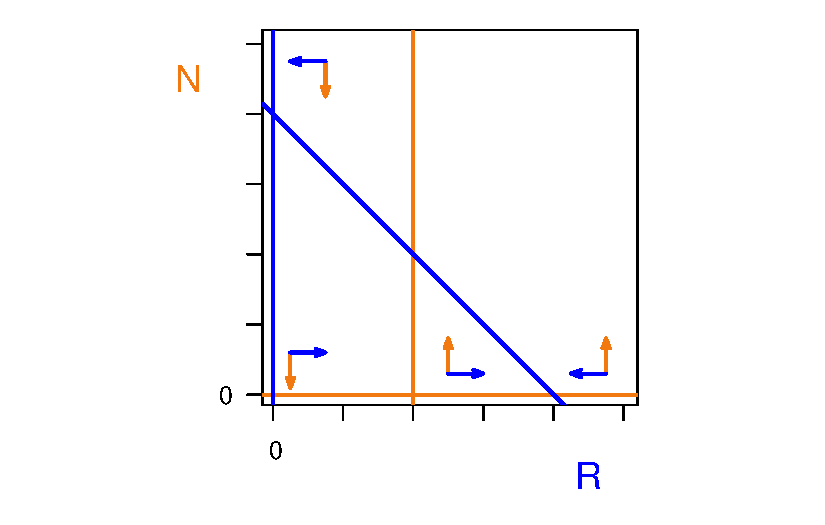
\includegraphics{Modellering/ecoevo_meerdere_files/figure-pdf/unnamed-chunk-6-1.pdf}

}

\end{figure}

Laten we even stil staan bij wat het diagram dat we net hebben
geconstrueerd eigenlijk betekent. In het diagram worden alle mogelijke
toetsanden weergegeven voor onze prooi- en predatordichtheden
(toestanden wordt ook wel fasen genoemd, vandaar het woord faseruimte).
Zo kun je aflezen hoe de populaties zullen veranderen over de tijd. In
het vorige hoofdstuk hebben we besproken dat het vinden van algemene
oplossingen (de functie die precies omschrijft hoe populaties
veranderen) vaak te moeilijk is. Voor het bovenstaande predator-prooi
model is dat zelfs \emph{onmogelijk}. Maar dit is toch juist wat we
willen weten? We willen toch juist weten hoe de populaties over de tijd
zullen veranderen? Gelukkig kunnen we met behulp van faseruimtes (zelfs
met pen en papier!) specifieke oplossingen aflezen. Dat wil zeggen:
gegeven een bepaalde begintoestand, waar zal het systeem zich heen
bewegen? In Figuur~\ref{fig-faseruimteoplossingenlv} zie je dat we op
die manier een ``trajectorie'' door de ruimte kunnen tekenen, wat direct
vertaalt in een specifieke oplossing! Dus met minimaal rekenwerk, kunnen
we toch voorspellen wat het systeem gaat doen!

\begin{figure}

{\centering 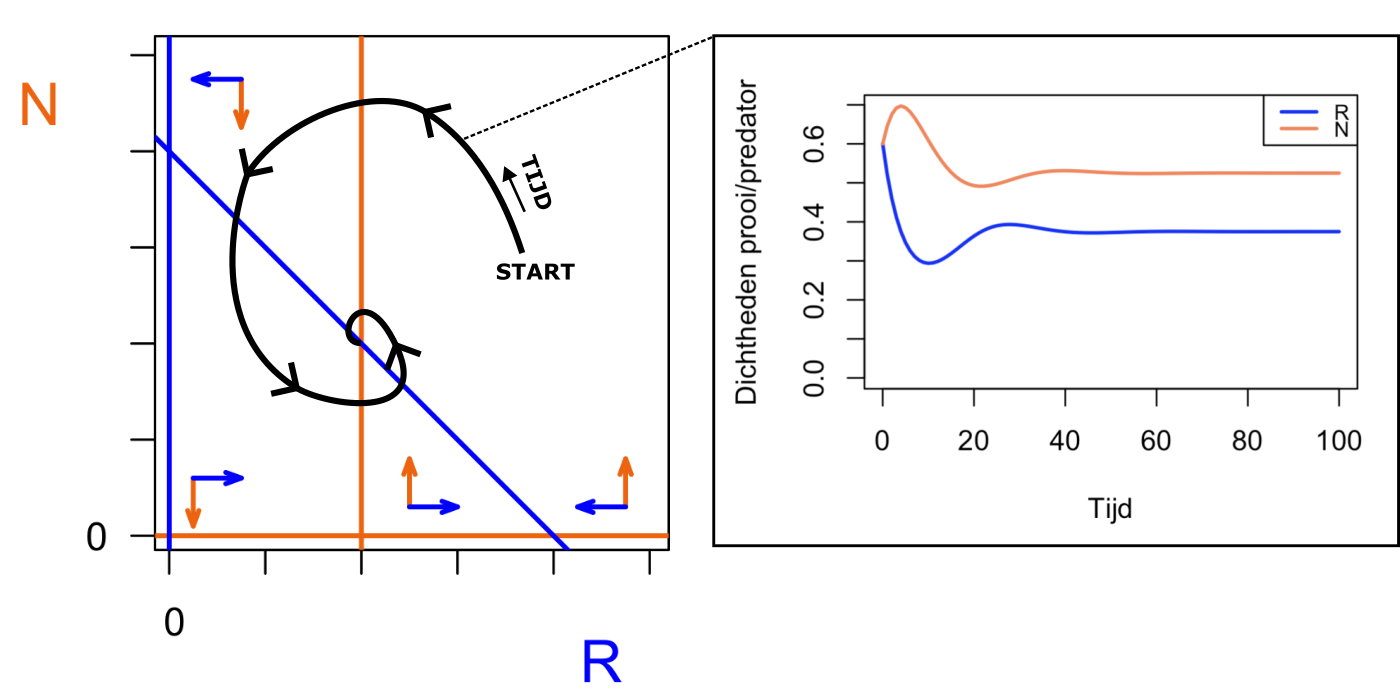
\includegraphics{Modellering/figuren/trajectory_LV.png}

}

\caption{\label{fig-faseruimteoplossingenlv}Vanuit een faseruimte kunnen
we aflezen hoe de populaties zich door de tijd zullen veranderen, en zo
specifieke oplossingen schetsen!}

\end{figure}

\hypertarget{stabiele-en-instabiele-evenwichten-in-2d-systemen}{%
\section{Stabiele en instabiele evenwichten in 2D
systemen}\label{stabiele-en-instabiele-evenwichten-in-2d-systemen}}

Zoals je ziet spiraliseert het systeem in
Figuur~\ref{fig-faseruimteoplossingenlv} richting het kruispunt tussen
de twee nullclines. Dit is ook wel logisch, want de nullclines geven aan
waar de populaties niet meer veranderen, dus het snijpunt geeft aan waar
ze \emph{beiden} niet meer veranderen. Maar zoals we voor 1D systemen
geleerd hebben: niet elke evenwichtsituatie is stabiel. Met andere
woorden, niet elk snijpunt van twee nullclines is ook een
\textbf{attractor} van het systeem. Hoe kunnen we aflezen of een
evenwicht stabiel of instabiel is? Om dit te bepalen, moeten we voor elk
evenwicht analyseren wat er rond het evenwicht gebeurt. Laten we
beginnen met alle evenwichten annoteren met een nummer:

\begin{Shaded}
\begin{Highlighting}[]
\CommentTok{\#| fig.width: 7}

\CommentTok{\#| fig.height: 4}

\CommentTok{\#| label: "fig{-}faseruimtecompleet"}

\CommentTok{\#| fig{-}cap: "Complete fase{-}ruimte van het predator{-}prooi systeem, waarbij open cirkels instabiele evenwichten weergeven, en het stabiele evenwicht is weergegeven met een gesloten (ingevulde) cirkel"}

\CommentTok{\#| code{-}fold: true}

\NormalTok{vectorfield }\OtherTok{\textless{}{-}} \ControlFlowTok{function}\NormalTok{(x,y,dx,dy)\{}

  \FunctionTok{arrows}\NormalTok{(x, y, x}\SpecialCharTok{+}\DecValTok{0}\NormalTok{, y}\SpecialCharTok{+}\NormalTok{dy, }\AttributeTok{length =} \FloatTok{0.07}\NormalTok{, }\AttributeTok{angle =} \DecValTok{20}\NormalTok{, }\AttributeTok{col=}\StringTok{"\#f2790f"}\NormalTok{,}\AttributeTok{lwd=}\DecValTok{2}\NormalTok{)}

  \FunctionTok{arrows}\NormalTok{(x, y, x}\SpecialCharTok{+}\NormalTok{dx, y}\SpecialCharTok{+}\DecValTok{0}\NormalTok{, }\AttributeTok{length =} \FloatTok{0.07}\NormalTok{, }\AttributeTok{angle =} \DecValTok{20}\NormalTok{, }\AttributeTok{col=}\StringTok{"blue"}\NormalTok{,}\AttributeTok{lwd=}\DecValTok{2}\NormalTok{)}

\NormalTok{\}}

\NormalTok{N }\OtherTok{\textless{}{-}} \DecValTok{1}\SpecialCharTok{:}\DecValTok{100}

\NormalTok{R }\OtherTok{\textless{}{-}} \DecValTok{1}\SpecialCharTok{:}\DecValTok{100}

\FunctionTok{par}\NormalTok{(}\AttributeTok{pty=}\StringTok{"s"}\NormalTok{,}\AttributeTok{mfrow=}\FunctionTok{c}\NormalTok{(}\DecValTok{1}\NormalTok{,}\DecValTok{1}\NormalTok{),}\AttributeTok{mar=}\FunctionTok{c}\NormalTok{(}\DecValTok{4}\NormalTok{,}\DecValTok{4}\NormalTok{,}\DecValTok{1}\NormalTok{,}\FloatTok{1.5}\NormalTok{))}

\FunctionTok{plot}\NormalTok{(R,N,  }\AttributeTok{col.axis=}\StringTok{"\#f2790f"}\NormalTok{,}\AttributeTok{type=}\StringTok{\textquotesingle{}n\textquotesingle{}}\NormalTok{,}\AttributeTok{xaxt=}\StringTok{\textquotesingle{}n\textquotesingle{}}\NormalTok{,}\AttributeTok{xlab=}\StringTok{""}\NormalTok{,}\AttributeTok{ylab=}\StringTok{""}\NormalTok{,}\AttributeTok{axes=}\ConstantTok{FALSE}\NormalTok{, }\AttributeTok{frame.plot=}\ConstantTok{TRUE}\NormalTok{)}

\FunctionTok{mtext}\NormalTok{(}\StringTok{"R"}\NormalTok{, }\AttributeTok{side=}\DecValTok{1}\NormalTok{, }\AttributeTok{line=}\DecValTok{2}\NormalTok{, }\AttributeTok{col=}\StringTok{"blue"}\NormalTok{, }\AttributeTok{cex=}\FloatTok{1.5}\NormalTok{, }\AttributeTok{at=}\DecValTok{90}\NormalTok{)}

\FunctionTok{mtext}\NormalTok{(}\StringTok{"N"}\NormalTok{, }\AttributeTok{side=}\DecValTok{2}\NormalTok{, }\AttributeTok{line=}\DecValTok{2}\NormalTok{, }\AttributeTok{col=}\StringTok{"\#f2790f"}\NormalTok{, }\AttributeTok{cex=}\FloatTok{1.5}\NormalTok{,}\AttributeTok{adj=}\DecValTok{1}\NormalTok{,}\AttributeTok{las=}\DecValTok{2}\NormalTok{, }\AttributeTok{at=}\DecValTok{90}\NormalTok{)}

\FunctionTok{mtext}\NormalTok{(}\StringTok{"0"}\NormalTok{, }\AttributeTok{side=}\DecValTok{2}\NormalTok{, }\AttributeTok{line=}\DecValTok{1}\NormalTok{, }\AttributeTok{col=}\StringTok{"black"}\NormalTok{, }\AttributeTok{cex=}\DecValTok{1}\NormalTok{,}\AttributeTok{adj=}\DecValTok{1}\NormalTok{,}\AttributeTok{las=}\DecValTok{2}\NormalTok{, }\AttributeTok{at=}\DecValTok{0}\NormalTok{)}

\FunctionTok{mtext}\NormalTok{(}\StringTok{"0"}\NormalTok{, }\AttributeTok{side=}\DecValTok{1}\NormalTok{, }\AttributeTok{line=}\DecValTok{1}\NormalTok{, }\AttributeTok{col=}\StringTok{"black"}\NormalTok{, }\AttributeTok{cex=}\DecValTok{1}\NormalTok{,}\AttributeTok{adj=}\DecValTok{0}\NormalTok{,}\AttributeTok{las=}\DecValTok{1}\NormalTok{, }\AttributeTok{at=}\SpecialCharTok{{-}}\DecValTok{1}\NormalTok{)}

\FunctionTok{Axis}\NormalTok{(}\AttributeTok{side=}\DecValTok{1}\NormalTok{, }\AttributeTok{labels=}\ConstantTok{FALSE}\NormalTok{)}

\FunctionTok{Axis}\NormalTok{(}\AttributeTok{side=}\DecValTok{2}\NormalTok{, }\AttributeTok{labels=}\ConstantTok{FALSE}\NormalTok{)}

\FunctionTok{vectorfield}\NormalTok{(}\DecValTok{5}\NormalTok{,}\DecValTok{22}\NormalTok{,}\DecValTok{10}\NormalTok{,}\SpecialCharTok{{-}}\DecValTok{10}\NormalTok{)}

\FunctionTok{vectorfield}\NormalTok{(}\DecValTok{95}\NormalTok{,}\DecValTok{16}\NormalTok{,}\SpecialCharTok{{-}}\DecValTok{10}\NormalTok{,}\DecValTok{10}\NormalTok{)}

\FunctionTok{vectorfield}\NormalTok{(}\DecValTok{50}\NormalTok{,}\DecValTok{6}\NormalTok{,}\DecValTok{10}\NormalTok{,}\DecValTok{10}\NormalTok{)}

\FunctionTok{vectorfield}\NormalTok{(}\DecValTok{15}\NormalTok{,}\DecValTok{95}\NormalTok{,}\SpecialCharTok{{-}}\DecValTok{10}\NormalTok{,}\SpecialCharTok{{-}}\DecValTok{10}\NormalTok{)}

 \FunctionTok{abline}\NormalTok{(}\AttributeTok{h=}\DecValTok{0}\NormalTok{, }\AttributeTok{lwd=}\DecValTok{2}\NormalTok{, }\AttributeTok{col=}\StringTok{"\#f2790f"}\NormalTok{)}

 \FunctionTok{abline}\NormalTok{(}\AttributeTok{v=}\DecValTok{40}\NormalTok{, }\AttributeTok{lwd=}\DecValTok{2}\NormalTok{, }\AttributeTok{col=}\StringTok{"\#f2790f"}\NormalTok{)}

 \FunctionTok{abline}\NormalTok{(}\AttributeTok{v=}\DecValTok{0}\NormalTok{, }\AttributeTok{lwd=}\DecValTok{2}\NormalTok{, }\AttributeTok{col=}\StringTok{"blue"}\NormalTok{,)}

 \FunctionTok{abline}\NormalTok{(}\AttributeTok{a=}\DecValTok{80}\NormalTok{,}\AttributeTok{b=}\SpecialCharTok{{-}}\DecValTok{1}\NormalTok{, }\AttributeTok{lwd=}\DecValTok{2}\NormalTok{,}\AttributeTok{col=}\StringTok{"blue"}\NormalTok{)}

 \FunctionTok{points}\NormalTok{(}\DecValTok{40}\NormalTok{,}\DecValTok{40}\NormalTok{,}\AttributeTok{cex=}\FloatTok{1.3}\NormalTok{,}\AttributeTok{pch=}\DecValTok{19}\NormalTok{)}

\FunctionTok{text}\NormalTok{(}\DecValTok{55}\NormalTok{,}\DecValTok{45}\NormalTok{,}\StringTok{"Evenwicht 3"}\NormalTok{, }\AttributeTok{cex=}\FloatTok{0.7}\NormalTok{)}

\FunctionTok{points}\NormalTok{(}\DecValTok{0}\NormalTok{,}\DecValTok{0}\NormalTok{,}\AttributeTok{cex=}\FloatTok{1.3}\NormalTok{)}

\FunctionTok{text}\NormalTok{(}\DecValTok{15}\NormalTok{,}\DecValTok{5}\NormalTok{,}\StringTok{"Evenwicht 1"}\NormalTok{, }\AttributeTok{cex=}\FloatTok{0.7}\NormalTok{)}

\FunctionTok{points}\NormalTok{(}\DecValTok{80}\NormalTok{,}\DecValTok{0}\NormalTok{,}\AttributeTok{cex=}\FloatTok{1.3}\NormalTok{)}

\FunctionTok{text}\NormalTok{(}\DecValTok{90}\NormalTok{,}\DecValTok{8}\NormalTok{,}\StringTok{"Evenwicht 2"}\NormalTok{, }\AttributeTok{cex=}\FloatTok{0.7}\NormalTok{)}
\end{Highlighting}
\end{Shaded}

\begin{figure}[H]

{\centering 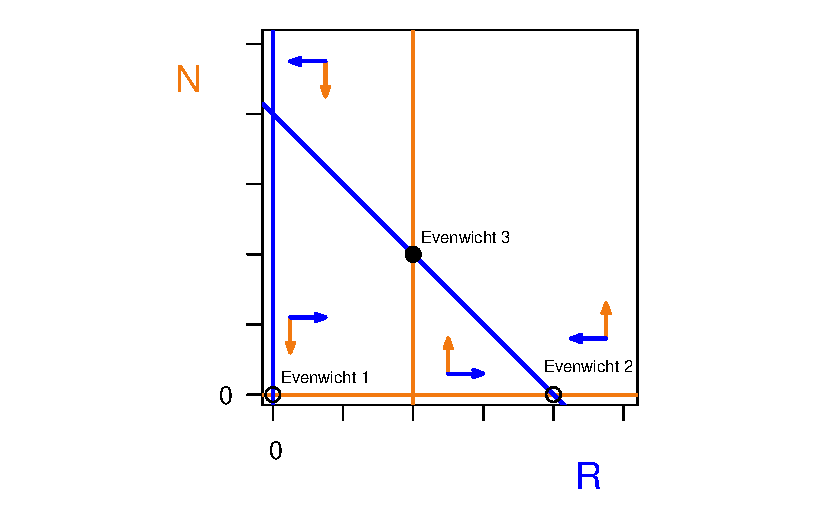
\includegraphics{Modellering/ecoevo_meerdere_files/figure-pdf/unnamed-chunk-7-1.pdf}

}

\end{figure}

Laten we beginnen bij evenwicht 1, waar beide populaties 0 zijn. Een
dergelijk evenwicht noemen we triviaal, omdat geen van de relevante
variabelen (predator/prooi) aanwezig is. In dit punt is er dus ook geen
verandering in de prooi- en predatorpopulatie. Maar wat als we een
beetje predator toevoegen? Kan de predator dan groeien? In dit geval
kijken we vlak boven het evenwicht, want dat is het punt waar er ``een
beetje predator'' aanwezig is. We zien dat in dit gebied de oranje pijl
naar beneden wijst, dus kan de predator alleen maar krimpen. Biologisch
betekent dit hetvolgende: predatoren kunnen niet groeien als er geen
prooien zijn (dit is het equivalent van vossen vrijlaten op Australië
voordat er konijnen waren!). We moeten natuurlijk ook controleren wat er
gebeurt als we een beetje prooi toevoegen. Om dit te bestuderen, kijken
we rechts van dit evenwicht. Hier is de groeisnelheid van de prooi
positief, en kan de prooipopulatie dus gaan groeien (ook dit is logisch,
want dit is precies wat er gebeurde met de vrijgelaten konijnen in
Australië!). Een evenwicht is alleen stabiel als het systeem na elke
verstoring terug gaat naar het evenwicht. Dus we moeten we hierbij
concluderen dat dit evenwicht \textbf{instabiel} is.

Voor evenwicht 2 en 3 kunnen we dezelfde analyse toepassen. Prooi
toevoegen aan evenwicht 2 resulteert in afname van de prooipopulatie,
maar predator toevoegen resulteert in toename van de predator.
Vergelijkbaar met evenwicht 1 is ook dit een \emph{instabiel evenwicht}.
Voor evenwicht 3 geldt wederom dat prooi toevoegen resulteert in afname.
Echter zien we dat we bij het toevoegen van predatoren (vlak boven
evenwicht 3) precies \emph{op} de nullcline zitten, en de groeisnelheid
van de predator dus 0 blijft. Omdat evenwicht 3 robust is voor het
toevoegen van prooi (de verstoring neemt af) en ook voor het toevoegen
van predator (de verstoring vergoot in ieder geval niet), kunnen we
concluderen dat dit evenwicht \textbf{stabiel} is. Daarom staat hij in
figuur \textbf{?@fig-faseruimtecompleet} aangegeven met een gesloten
cirkel.

\hypertarget{verhoogde-death-rates-van-predatoren}{%
\section{Verhoogde death rates van
predatoren}\label{verhoogde-death-rates-van-predatoren}}

Nu we onze faseruimte hebben uitgewerkt, is het heel makkelijk om
biologisch relevante vragen te stellen. We zouden ons bijvoorbeeld af
kunnen vragen wat er gebeurt met een verhoogde sterfte van de
predatoren. Om het effect hiervan te begrijpen, kijken we naar de
vergelijkingen voor de nullclines:

\begin{align*}
    \color{blue}R_{1}\color{black} \rightarrow \color{blue}R &= 0 \\
    \color{blue}R_{2}\color{black} \rightarrow \color{orange}N\color{black} &= \frac{b(1-\frac{\color{blue}R}{K})\color{black} - d}{a} \\
    \color{orange}N_{1}\color{black} \rightarrow \color{orange}N\color{black} &= 0 \\
    \color{orange}N_{2}\color{black} \rightarrow \frac{\delta}{ca}
\end{align*}

\begin{tcolorbox}[enhanced jigsaw, coltitle=black, breakable, bottomtitle=1mm, opacityback=0, colback=white, rightrule=.15mm, title=\textcolor{quarto-callout-warning-color}{\faExclamationTriangle}\hspace{0.5em}{Een nullclines gegeven door X = \ldots, is niet altijd de nullcline voor
X!}, bottomrule=.15mm, toprule=.15mm, left=2mm, colframe=quarto-callout-warning-color-frame, toptitle=1mm, opacitybacktitle=0.6, titlerule=0mm, colbacktitle=quarto-callout-warning-color!10!white, leftrule=.75mm, arc=.35mm]

Bij nullclines heb je vaak te maken met twee variabelen, dus kun je ze
op meerdere manieren opschrijven. Bijvoorbeeld, de vergelijkingen
\(y=x^2\) en \(x=\sqrt(y)\) bevatten dezelfde informatie en zien er
hetzelfde uit in een grafiek.

Het is vaak handig om nullclines op te schrijven als functie van de
variabele op de x-as (in het predator-prooi systeem, schrijven we dus
\(N=f(R)\)). Dit is omdat we gewend zijn om y als functie van x te
schetsen, en niet andersom. Dit is een conventie en kan omgedraaid
worden --- de prooi hoeft natuurlijk niet op de x-as te staan!

\end{tcolorbox}

Kijkende naar de vier nullclines hierboven, kunnen we zien dat slechts 1
ervan afhangt van de sterfte van predatoren (\(\delta\)). Als deze
verhoogd, wordt de fractie \(\frac{\delta}{ca}\) hoger, en verschuift
dus de nullcline naar rechts. Let op! Dit zal ook veranderen hoe het
vectorveld precies loopt, en waar eventuele snijpunten liggen! In
Figuur~\ref{fig-predatordeath} a) zie je hoe de nieuwe faseruimte eruit
ziet, en dat er geen stabiel evenwicht meer is voor zowel predator als
prooi. In plaats daarvan is er alleen een evenwicht met prooi
overgebleven, en hoewel dit evenwicht voorheen instabiel was, is deze nu
(kijkend naar het vectorveld) stabiel geworden! Dus: als de death rate
te hoog is kunnen predatoren (zoals je eigenlijk wel verwacht) niet
overleven. Maar let op, niet elke parameter-verandering heeft intuïtieve
effecten! Als we bijvoorbeeld dezelde analyse doen voor een verhoogde
birth rate van de prooi (Figuur~\ref{fig-predatordeath} b), zien we dat
er in evenwicht precies evenveel prooien zullen zijn, en alleen maar
meer predatoren!

\begin{Shaded}
\begin{Highlighting}[]
\NormalTok{N }\OtherTok{\textless{}{-}} \DecValTok{1}\SpecialCharTok{:}\DecValTok{100}
\NormalTok{R }\OtherTok{\textless{}{-}} \DecValTok{1}\SpecialCharTok{:}\DecValTok{100}

\FunctionTok{par}\NormalTok{(}\AttributeTok{pty=}\StringTok{"s"}\NormalTok{,}\AttributeTok{mfrow=}\FunctionTok{c}\NormalTok{(}\DecValTok{1}\NormalTok{,}\DecValTok{1}\NormalTok{),}\AttributeTok{mar=}\FunctionTok{c}\NormalTok{(}\DecValTok{4}\NormalTok{,}\FloatTok{3.3}\NormalTok{,}\DecValTok{1}\NormalTok{,}\DecValTok{1}\NormalTok{))}
\FunctionTok{plot}\NormalTok{(R,N,  }\AttributeTok{col.axis=}\StringTok{"\#FF7F50"}\NormalTok{,}\AttributeTok{type=}\StringTok{\textquotesingle{}n\textquotesingle{}}\NormalTok{,}\AttributeTok{xaxt=}\StringTok{\textquotesingle{}n\textquotesingle{}}\NormalTok{,}\AttributeTok{xlab=}\StringTok{""}\NormalTok{,}\AttributeTok{ylab=}\StringTok{""}\NormalTok{,}\AttributeTok{axes=}\ConstantTok{FALSE}\NormalTok{, }\AttributeTok{frame.plot=}\ConstantTok{TRUE}\NormalTok{)}
\FunctionTok{mtext}\NormalTok{(}\StringTok{"R"}\NormalTok{, }\AttributeTok{font=}\DecValTok{2}\NormalTok{,}\AttributeTok{side=}\DecValTok{1}\NormalTok{, }\AttributeTok{line=}\DecValTok{2}\NormalTok{, }\AttributeTok{col=}\StringTok{"blue"}\NormalTok{, }\AttributeTok{cex=}\FloatTok{1.5}\NormalTok{, }\AttributeTok{at=}\DecValTok{90}\NormalTok{)}
\FunctionTok{mtext}\NormalTok{(}\StringTok{"N"}\NormalTok{, }\AttributeTok{font=}\DecValTok{2}\NormalTok{,}\AttributeTok{side=}\DecValTok{2}\NormalTok{, }\AttributeTok{line=}\DecValTok{2}\NormalTok{, }\AttributeTok{col=}\StringTok{"\#FF7F50"}\NormalTok{, }\AttributeTok{cex=}\FloatTok{1.5}\NormalTok{,}\AttributeTok{adj=}\DecValTok{1}\NormalTok{,}\AttributeTok{las=}\DecValTok{2}\NormalTok{, }\AttributeTok{at=}\DecValTok{90}\NormalTok{)}
\FunctionTok{mtext}\NormalTok{(}\StringTok{"0"}\NormalTok{, }\AttributeTok{font=}\DecValTok{2}\NormalTok{,}\AttributeTok{side=}\DecValTok{2}\NormalTok{, }\AttributeTok{line=}\DecValTok{1}\NormalTok{, }\AttributeTok{col=}\StringTok{"black"}\NormalTok{, }\AttributeTok{cex=}\DecValTok{1}\NormalTok{,}\AttributeTok{adj=}\DecValTok{1}\NormalTok{,}\AttributeTok{las=}\DecValTok{2}\NormalTok{, }\AttributeTok{at=}\DecValTok{0}\NormalTok{)}
\FunctionTok{mtext}\NormalTok{(}\StringTok{"0"}\NormalTok{, }\AttributeTok{font=}\DecValTok{2}\NormalTok{,}\AttributeTok{side=}\DecValTok{1}\NormalTok{, }\AttributeTok{line=}\DecValTok{1}\NormalTok{, }\AttributeTok{col=}\StringTok{"black"}\NormalTok{, }\AttributeTok{cex=}\DecValTok{1}\NormalTok{,}\AttributeTok{adj=}\DecValTok{0}\NormalTok{,}\AttributeTok{las=}\DecValTok{1}\NormalTok{, }\AttributeTok{at=}\SpecialCharTok{{-}}\DecValTok{1}\NormalTok{)}
\FunctionTok{Axis}\NormalTok{(}\AttributeTok{side=}\DecValTok{1}\NormalTok{, }\AttributeTok{labels=}\ConstantTok{FALSE}\NormalTok{)}
\FunctionTok{Axis}\NormalTok{(}\AttributeTok{side=}\DecValTok{2}\NormalTok{, }\AttributeTok{labels=}\ConstantTok{FALSE}\NormalTok{)}
\FunctionTok{abline}\NormalTok{(}\AttributeTok{h=}\DecValTok{0}\NormalTok{, }\AttributeTok{lwd=}\DecValTok{3}\NormalTok{, }\AttributeTok{col=}\StringTok{"\#FF7F50"}\NormalTok{)}
\FunctionTok{abline}\NormalTok{(}\AttributeTok{v=}\DecValTok{40}\NormalTok{, }\AttributeTok{lwd=}\DecValTok{2}\NormalTok{, }\AttributeTok{col=}\StringTok{"\#FF7F50"}\NormalTok{, }\AttributeTok{lty=}\DecValTok{8}\NormalTok{)}
\FunctionTok{arrows}\NormalTok{(}\DecValTok{45}\NormalTok{, }\DecValTok{70}\NormalTok{, }\DecValTok{85}\NormalTok{, }\DecValTok{70}\NormalTok{, }\AttributeTok{length =} \FloatTok{0.07}\NormalTok{, }\AttributeTok{angle =} \DecValTok{20}\NormalTok{, }\AttributeTok{col=}\StringTok{"grey"}\NormalTok{,}\AttributeTok{lwd=}\DecValTok{2}\NormalTok{)}
\FunctionTok{text}\NormalTok{(}\DecValTok{65}\NormalTok{,}\DecValTok{80}\NormalTok{,}\StringTok{"Verschuiving }\SpecialCharTok{\textbackslash{}n}\StringTok{predator{-}nullcline"}\NormalTok{,}\AttributeTok{cex=}\FloatTok{0.7}\NormalTok{)}
\FunctionTok{mtext}\NormalTok{(}\StringTok{"Effect hogere death rate predator"}\NormalTok{, }\AttributeTok{font=}\DecValTok{2}\NormalTok{,}\AttributeTok{side=}\DecValTok{3}\NormalTok{, }\AttributeTok{line=}\DecValTok{1}\NormalTok{, }\AttributeTok{col=}\StringTok{"black"}\NormalTok{, }\AttributeTok{cex=}\FloatTok{1.0}\NormalTok{, }\AttributeTok{at=}\DecValTok{50}\NormalTok{)}
\FunctionTok{abline}\NormalTok{(}\AttributeTok{v=}\DecValTok{90}\NormalTok{, }\AttributeTok{lwd=}\DecValTok{3}\NormalTok{, }\AttributeTok{col=}\StringTok{"\#FF7F50"}\NormalTok{)}
\FunctionTok{abline}\NormalTok{(}\AttributeTok{v=}\DecValTok{0}\NormalTok{, }\AttributeTok{lwd=}\DecValTok{3}\NormalTok{, }\AttributeTok{col=}\StringTok{"blue"}\NormalTok{)}
\FunctionTok{abline}\NormalTok{(}\AttributeTok{a=}\DecValTok{80}\NormalTok{,}\AttributeTok{b=}\SpecialCharTok{{-}}\DecValTok{1}\NormalTok{, }\AttributeTok{lwd=}\DecValTok{3}\NormalTok{,}\AttributeTok{col=}\StringTok{"blue"}\NormalTok{)}
\FunctionTok{points}\NormalTok{(}\DecValTok{0}\NormalTok{,}\DecValTok{0}\NormalTok{,}\AttributeTok{cex=}\FloatTok{1.3}\NormalTok{)}
\FunctionTok{points}\NormalTok{(}\DecValTok{80}\NormalTok{,}\DecValTok{0}\NormalTok{,}\AttributeTok{cex=}\FloatTok{1.3}\NormalTok{,}\AttributeTok{pch=}\DecValTok{19}\NormalTok{)}
\NormalTok{add\_vector }\OtherTok{\textless{}{-}} \ControlFlowTok{function}\NormalTok{(x,y,dx,dy)\{}
  \FunctionTok{arrows}\NormalTok{(x, y, x}\SpecialCharTok{+}\NormalTok{dx, y, }\AttributeTok{length =} \FloatTok{0.07}\NormalTok{, }\AttributeTok{angle =} \DecValTok{20}\NormalTok{, }\AttributeTok{col=}\StringTok{"blue"}\NormalTok{,}\AttributeTok{lwd=}\DecValTok{2}\NormalTok{)}
  \FunctionTok{arrows}\NormalTok{(x, y, x, y}\SpecialCharTok{+}\NormalTok{dy, }\AttributeTok{length =} \FloatTok{0.07}\NormalTok{, }\AttributeTok{angle =} \DecValTok{20}\NormalTok{, }\AttributeTok{col=}\StringTok{"\#FF7F50"}\NormalTok{,}\AttributeTok{lwd=}\DecValTok{2}\NormalTok{)}
\NormalTok{\}}

\FunctionTok{add\_vector}\NormalTok{(}\DecValTok{10}\NormalTok{,}\DecValTok{20}\NormalTok{,}\DecValTok{10}\NormalTok{,}\SpecialCharTok{{-}}\DecValTok{10}\NormalTok{)}
\FunctionTok{add\_vector}\NormalTok{(}\DecValTok{85}\NormalTok{,}\DecValTok{30}\NormalTok{,}\SpecialCharTok{{-}}\DecValTok{10}\NormalTok{,}\SpecialCharTok{{-}}\DecValTok{10}\NormalTok{)}
\FunctionTok{add\_vector}\NormalTok{(}\DecValTok{102}\NormalTok{,}\DecValTok{20}\NormalTok{,}\SpecialCharTok{{-}}\DecValTok{10}\NormalTok{,}\DecValTok{10}\NormalTok{)}

\NormalTok{N }\OtherTok{\textless{}{-}} \DecValTok{1}\SpecialCharTok{:}\DecValTok{100}
\NormalTok{R }\OtherTok{\textless{}{-}} \DecValTok{1}\SpecialCharTok{:}\DecValTok{100}

\FunctionTok{plot}\NormalTok{(R,N,  }\AttributeTok{col.axis=}\StringTok{"\#FF7F50"}\NormalTok{,}\AttributeTok{type=}\StringTok{\textquotesingle{}n\textquotesingle{}}\NormalTok{,}\AttributeTok{xaxt=}\StringTok{\textquotesingle{}n\textquotesingle{}}\NormalTok{,}\AttributeTok{xlab=}\StringTok{""}\NormalTok{,}\AttributeTok{ylab=}\StringTok{""}\NormalTok{,}\AttributeTok{axes=}\ConstantTok{FALSE}\NormalTok{, }\AttributeTok{frame.plot=}\ConstantTok{TRUE}\NormalTok{)}

\FunctionTok{mtext}\NormalTok{(}\StringTok{"R"}\NormalTok{, }\AttributeTok{font=}\DecValTok{2}\NormalTok{,}\AttributeTok{side=}\DecValTok{1}\NormalTok{, }\AttributeTok{line=}\DecValTok{2}\NormalTok{, }\AttributeTok{col=}\StringTok{"blue"}\NormalTok{, }\AttributeTok{cex=}\FloatTok{1.5}\NormalTok{, }\AttributeTok{at=}\DecValTok{90}\NormalTok{)}
\FunctionTok{mtext}\NormalTok{(}\StringTok{"N"}\NormalTok{, }\AttributeTok{font=}\DecValTok{2}\NormalTok{,}\AttributeTok{side=}\DecValTok{2}\NormalTok{, }\AttributeTok{line=}\DecValTok{2}\NormalTok{, }\AttributeTok{col=}\StringTok{"\#FF7F50"}\NormalTok{, }\AttributeTok{cex=}\FloatTok{1.5}\NormalTok{,}\AttributeTok{adj=}\DecValTok{1}\NormalTok{,}\AttributeTok{las=}\DecValTok{2}\NormalTok{, }\AttributeTok{at=}\DecValTok{90}\NormalTok{)}
\FunctionTok{mtext}\NormalTok{(}\StringTok{"0"}\NormalTok{, }\AttributeTok{font=}\DecValTok{2}\NormalTok{,}\AttributeTok{side=}\DecValTok{2}\NormalTok{, }\AttributeTok{line=}\DecValTok{1}\NormalTok{, }\AttributeTok{col=}\StringTok{"black"}\NormalTok{, }\AttributeTok{cex=}\DecValTok{1}\NormalTok{,}\AttributeTok{adj=}\DecValTok{1}\NormalTok{,}\AttributeTok{las=}\DecValTok{2}\NormalTok{, }\AttributeTok{at=}\DecValTok{0}\NormalTok{)}
\FunctionTok{mtext}\NormalTok{(}\StringTok{"0"}\NormalTok{, }\AttributeTok{font=}\DecValTok{2}\NormalTok{,}\AttributeTok{side=}\DecValTok{1}\NormalTok{, }\AttributeTok{line=}\DecValTok{1}\NormalTok{, }\AttributeTok{col=}\StringTok{"black"}\NormalTok{, }\AttributeTok{cex=}\DecValTok{1}\NormalTok{,}\AttributeTok{adj=}\DecValTok{0}\NormalTok{,}\AttributeTok{las=}\DecValTok{1}\NormalTok{, }\AttributeTok{at=}\SpecialCharTok{{-}}\DecValTok{1}\NormalTok{)}

\FunctionTok{Axis}\NormalTok{(}\AttributeTok{side=}\DecValTok{1}\NormalTok{, }\AttributeTok{labels=}\ConstantTok{FALSE}\NormalTok{)}
\FunctionTok{Axis}\NormalTok{(}\AttributeTok{side=}\DecValTok{2}\NormalTok{, }\AttributeTok{labels=}\ConstantTok{FALSE}\NormalTok{)}

\FunctionTok{abline}\NormalTok{(}\AttributeTok{h=}\DecValTok{0}\NormalTok{, }\AttributeTok{lwd=}\DecValTok{3}\NormalTok{, }\AttributeTok{col=}\StringTok{"\#FF7F50"}\NormalTok{)}
\FunctionTok{abline}\NormalTok{(}\AttributeTok{v=}\DecValTok{40}\NormalTok{, }\AttributeTok{lwd=}\DecValTok{3}\NormalTok{, }\AttributeTok{col=}\StringTok{"\#FF7F50"}\NormalTok{)}

\FunctionTok{arrows}\NormalTok{(}\DecValTok{20}\NormalTok{, }\DecValTok{63}\NormalTok{, }\DecValTok{20}\NormalTok{, }\DecValTok{73}\NormalTok{, }\AttributeTok{length =} \FloatTok{0.07}\NormalTok{, }\AttributeTok{angle =} \DecValTok{20}\NormalTok{, }\AttributeTok{col=}\StringTok{"grey"}\NormalTok{,}\AttributeTok{lwd=}\DecValTok{2}\NormalTok{)}
\FunctionTok{text}\NormalTok{(}\DecValTok{20}\NormalTok{,}\DecValTok{45}\NormalTok{,}\StringTok{"Verschuiving }\SpecialCharTok{\textbackslash{}n}\StringTok{prooi{-}nullcline"}\NormalTok{,}\AttributeTok{cex=}\FloatTok{0.7}\NormalTok{)}

\FunctionTok{arrows}\NormalTok{(}\DecValTok{15}\NormalTok{,}\DecValTok{50}\NormalTok{,}\DecValTok{19}\NormalTok{,}\DecValTok{65}\NormalTok{,}\AttributeTok{length=}\DecValTok{0}\NormalTok{,}\AttributeTok{lty=}\DecValTok{3}\NormalTok{,}\AttributeTok{lwd=}\FloatTok{0.5}\NormalTok{)}
\FunctionTok{mtext}\NormalTok{(}\StringTok{"Effect hogere birth rate prooi"}\NormalTok{, }\AttributeTok{font=}\DecValTok{2}\NormalTok{,}\AttributeTok{side=}\DecValTok{3}\NormalTok{, }\AttributeTok{line=}\DecValTok{1}\NormalTok{, }\AttributeTok{col=}\StringTok{"black"}\NormalTok{, }\AttributeTok{cex=}\FloatTok{1.0}\NormalTok{, }\AttributeTok{at=}\DecValTok{50}\NormalTok{)}

\FunctionTok{abline}\NormalTok{(}\AttributeTok{v=}\DecValTok{0}\NormalTok{, }\AttributeTok{lwd=}\DecValTok{3}\NormalTok{, }\AttributeTok{col=}\StringTok{"blue"}\NormalTok{,)}
\FunctionTok{abline}\NormalTok{(}\AttributeTok{a=}\DecValTok{80}\NormalTok{,}\AttributeTok{b=}\SpecialCharTok{{-}}\DecValTok{1}\NormalTok{, }\AttributeTok{lwd=}\DecValTok{2}\NormalTok{,}\AttributeTok{lty=}\DecValTok{8}\NormalTok{,}\AttributeTok{col=}\StringTok{"blue"}\NormalTok{)}
\FunctionTok{abline}\NormalTok{(}\AttributeTok{a=}\DecValTok{100}\NormalTok{,}\AttributeTok{b=}\SpecialCharTok{{-}}\FloatTok{1.15}\NormalTok{, }\AttributeTok{lwd=}\DecValTok{3}\NormalTok{,}\AttributeTok{col=}\StringTok{"blue"}\NormalTok{)}

\FunctionTok{points}\NormalTok{(}\DecValTok{0}\NormalTok{,}\DecValTok{0}\NormalTok{,}\AttributeTok{cex=}\FloatTok{1.3}\NormalTok{)}
\FunctionTok{points}\NormalTok{(}\DecValTok{40}\NormalTok{,}\DecValTok{54}\NormalTok{,}\AttributeTok{cex=}\FloatTok{1.3}\NormalTok{,}\AttributeTok{pch=}\DecValTok{19}\NormalTok{)}
\FunctionTok{points}\NormalTok{(}\DecValTok{80}\NormalTok{,}\DecValTok{0}\NormalTok{,}\AttributeTok{cex=}\FloatTok{1.3}\NormalTok{)}

\NormalTok{add\_vector }\OtherTok{\textless{}{-}} \ControlFlowTok{function}\NormalTok{(x,y,dx,dy)\{}
  \FunctionTok{arrows}\NormalTok{(x, y, x}\SpecialCharTok{+}\NormalTok{dx, y, }\AttributeTok{length =} \FloatTok{0.07}\NormalTok{, }\AttributeTok{angle =} \DecValTok{20}\NormalTok{, }\AttributeTok{col=}\StringTok{"blue"}\NormalTok{,}\AttributeTok{lwd=}\DecValTok{2}\NormalTok{)}
  \FunctionTok{arrows}\NormalTok{(x, y, x, y}\SpecialCharTok{+}\NormalTok{dy, }\AttributeTok{length =} \FloatTok{0.07}\NormalTok{, }\AttributeTok{angle =} \DecValTok{20}\NormalTok{, }\AttributeTok{col=}\StringTok{"\#FF7F50"}\NormalTok{,}\AttributeTok{lwd=}\DecValTok{2}\NormalTok{)}
\NormalTok{\}}

\FunctionTok{add\_vector}\NormalTok{(}\DecValTok{10}\NormalTok{,}\DecValTok{30}\NormalTok{,}\DecValTok{10}\NormalTok{,}\SpecialCharTok{{-}}\DecValTok{10}\NormalTok{)}
\FunctionTok{add\_vector}\NormalTok{(}\DecValTok{50}\NormalTok{,}\DecValTok{10}\NormalTok{,}\DecValTok{10}\NormalTok{,}\DecValTok{10}\NormalTok{)}
\FunctionTok{add\_vector}\NormalTok{(}\DecValTok{30}\NormalTok{,}\DecValTok{95}\NormalTok{,}\SpecialCharTok{{-}}\DecValTok{10}\NormalTok{,}\SpecialCharTok{{-}}\DecValTok{10}\NormalTok{)}
\FunctionTok{add\_vector}\NormalTok{(}\DecValTok{90}\NormalTok{,}\DecValTok{30}\NormalTok{,}\SpecialCharTok{{-}}\DecValTok{10}\NormalTok{,}\DecValTok{10}\NormalTok{)}
\end{Highlighting}
\end{Shaded}

\begin{figure}

\begin{minipage}[t]{0.50\linewidth}

{\centering 

\raisebox{-\height}{

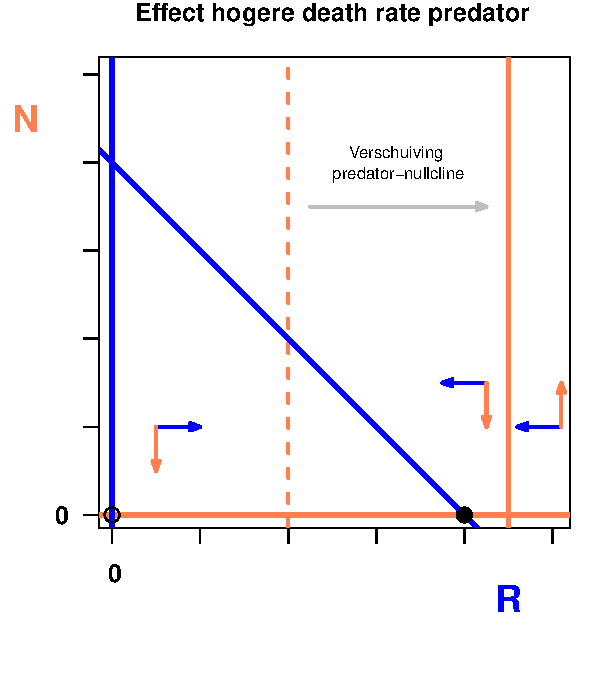
\includegraphics{Modellering/ecoevo_meerdere_files/figure-pdf/fig-predatordeath-1.pdf}

}

}

\subcaption{\label{fig-predatordeath-1}Effect van een verhoging van de
death rate van de predators zorgt dat de predator niet meer kan
overleven: een intuïtief resultaat!}
\end{minipage}%
%
\begin{minipage}[t]{0.50\linewidth}

{\centering 

\raisebox{-\height}{

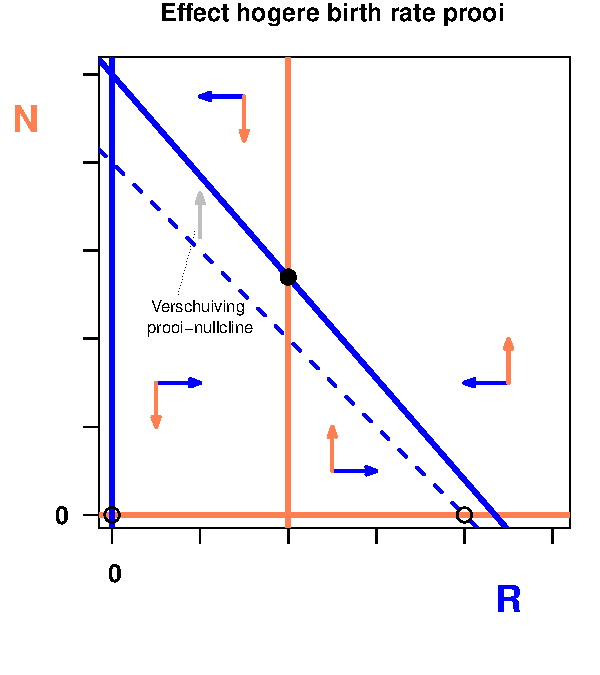
\includegraphics{Modellering/ecoevo_meerdere_files/figure-pdf/fig-predatordeath-2.pdf}

}

}

\subcaption{\label{fig-predatordeath-2}Effect van een verhoging van de
birth rate van de prooi levert alleen meer predatoren op: een
tegenintuïtief resultaat!}
\end{minipage}%

\caption{\label{fig-predatordeath}\textbf{?(caption)}}

\end{figure}

Op een vergelijkbare manier kunnen we het effect van andere
parameterveranderingen bestuderen. Zodoende kunnen ecologen voorspellen
of soorten dreigen uit te sterven, of epidemiologen voorspellen of een
virus zal uitbreiden \emph{etc.}

\hypertarget{opgaven-4}{%
\section{Opgaven}\label{opgaven-4}}

\begin{exercise}[Zieke
zeehonden]\protect\hypertarget{exr-ziekezeehonden}{}\label{exr-ziekezeehonden}

\begin{figure}

{\centering 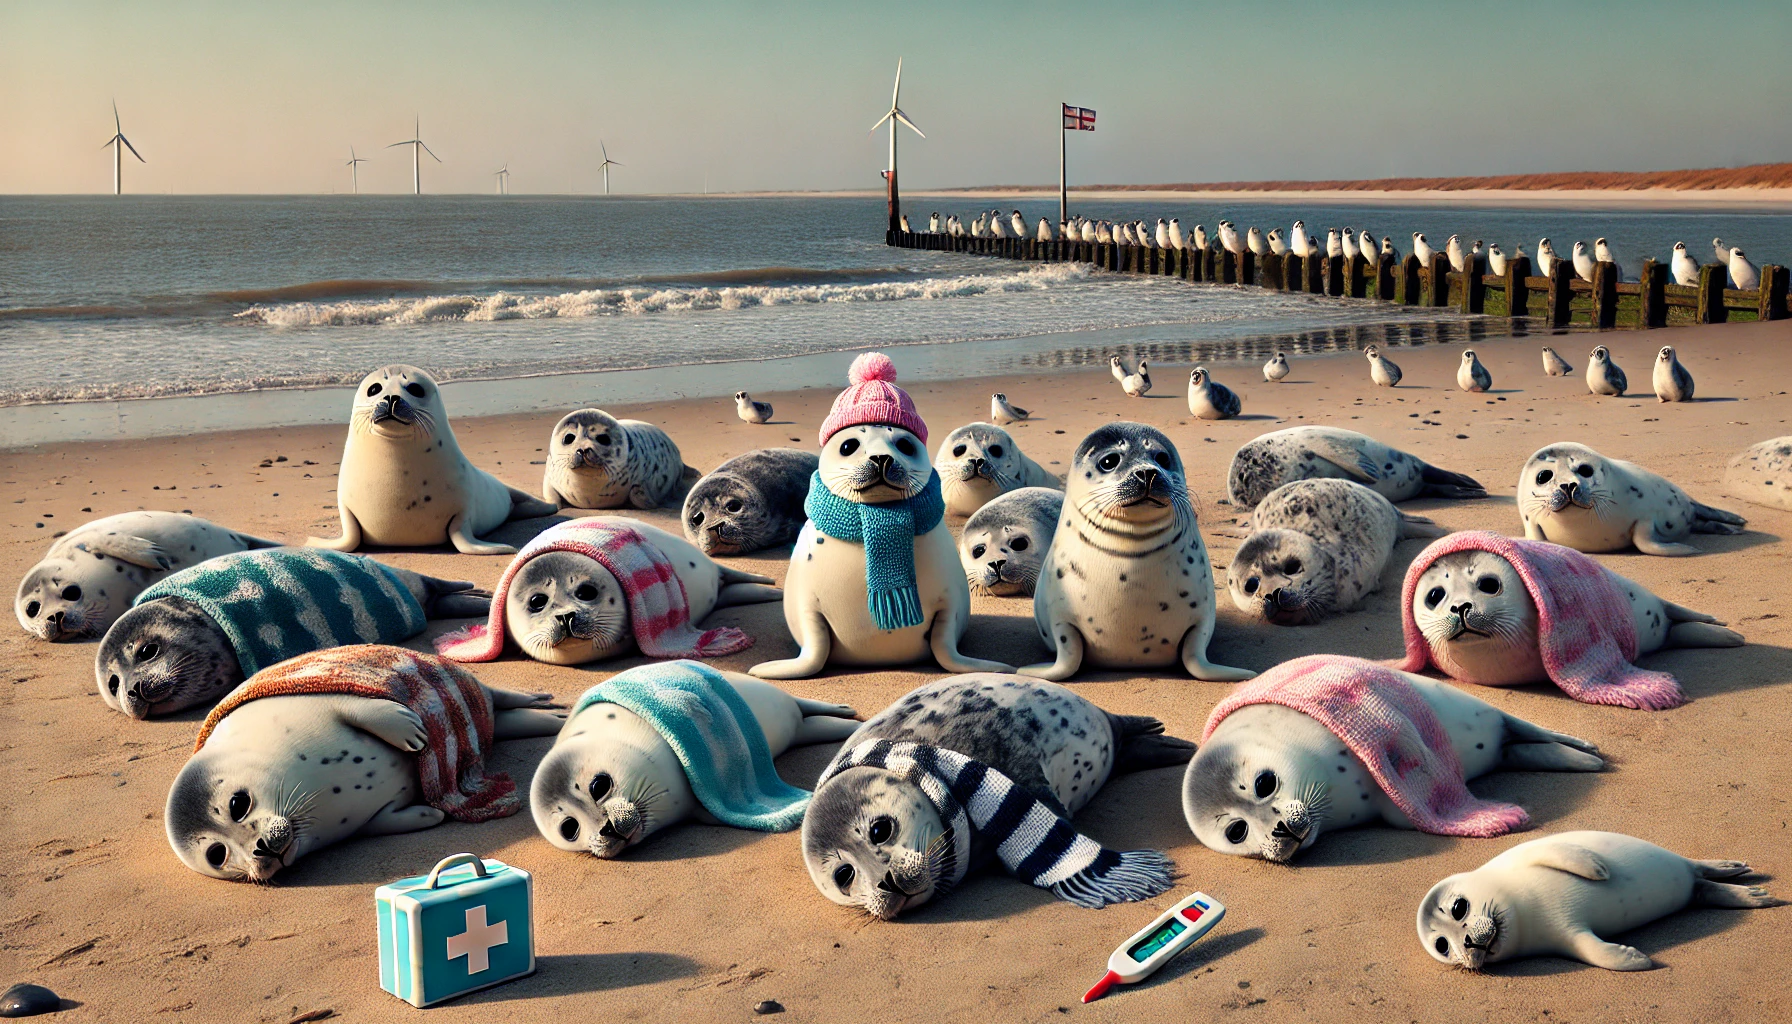
\includegraphics[width=0.8\textwidth,height=\textheight]{Modellering/figuren/zieke_zeehonden_AI.png}

}

\end{figure}

Laten we aannemen dat zeehonden (\(Z\)) op de waddenzee groeien met
dichtheidsafhankelijke geboorte (maximale geboorte \(b\),
dichtheidseffect \(k\)) en constante sterfte (\(d\)). We nemen aan dat
een deel van deze zeehonden geïnfecteerd wordt met een ziekte waardoor
ze na een korte tijd dood gaan. De geïnfecteerde zeehonden noemen we
\(I\):

\begin{align*}
\mathchoice{\frac{\mathrm{d}Z}
{\mathrm{d}t}}{\mathrm{d}Z/\mathrm{d}t}
{\mathrm{d}Z/\mathrm{d}t}
{\mathrm{d}Z/\mathrm{d}t} &= bZ(1-Z/k)-dZ-\beta ZI \text{,} \quad \text{en} \\
\mathchoice{\frac{\mathrm{d}I}
{\mathrm{d}t}}{\mathrm{d}I/\mathrm{d}t}
{\mathrm{d}I/\mathrm{d}t}
{\mathrm{d}I/\mathrm{d}t} &= \beta ZI - \delta I \quad \text{met } \delta \gg d
\end{align*}

\begin{enumerate}
\def\labelenumi{\alph{enumi}.}
\item
  Waar staan de parameters \(\beta\) en \(\delta\) voor? Hoe zou je de
  \(\beta ZI\) term noemen? \emph{ANTWOORD: De
  infectiesnelheid-parameter noemen we \(\beta\), en de sterfte van
  gezonde zeehonden noemen we \(\delta\). De term is dus een
  infectie-term}
\item
  Naast de ODE voor \(I\) staat een extra aanname, namelijk
  \(\delta \gg d\). Gegeven de modelomschrijving hierboven, vind je dit
  een redelijke aanname? \emph{ANTWOORD ja, wel gegeven de
  modelomschrijving. de zeehonden die ziek zijn zouden snel dood moeten
  gaan volgens de modelomschrijving}
\item
  We gaan eerst het model bekijken zonder infectie. Als er geen infectie
  aanwezig is (\(I=0\)), versimpeld de vergelijking in een 1D
  populatiegroei model. Wat zijn in dit geval de evenwichten van de
  gezonde zeehondenpopulatie? \emph{k(1-d/b)}
\item
  PCB's (polychloorbifenylen) zijn schadelijke stoffen die de
  geboortesnelheid van zeehonden kunnen beinvloeden. Stel dat er
  nogsteeds geen infectie aanwezig is, en dat de PCB's de
  geboortesnelheid (\(b\)) halveren. Wordt de populatie gezonde
  zeehonden kleiner? \emph{ANTWOORD: ja, k(1-d/b) met kleinere b, dus
  grotere d/b, dus kleiner totaal. dus de populatie zal afnamen als b
  kleiner wordt.}
\item
  We gaan bestuderen wat er gebeurt als er een ziekte wordt
  geïntroduceerd in deze populatie. Om het 2D systeem te analyseren,
  maken we een faseruimte. Zet de gezonde zeehonden op de x-as, en de
  zieke zeehonden op de y-as. Schets twee kwalitatief verschillende
  faseruimtes en trajectories: één waar de ziekte verspreidt en de
  zeehonden chronisch geinfecteerd blijven, en één waar de ziekte
  uitsterft. Bestudeer de stabiliteit van alle evenwichten
  \emph{ANTWOORD:werk dit goed uit!}
\item
  Welke parameters bepalen in welk scenario van de vorige vraag we ons
  bevinden? \emph{ANTWOORD:beta en delta}
\item
  Ga er opnieuw vanuit dat PCB's de geboorte van gezonde zeehonden
  (\(b\)) halveren, en schets de nieuwe nullcline samen met de oude
  nullcline in 1 faseruimte. \emph{ANTWOORD:een normale schuine lijn
  voor Z, en eentje die lager ligt.}
\item
  Hoeveel kleiner wordt de gezonde zeehondenpopulatie in evenwicht?
  \emph{ANTWOORD: helemaal niet kleiner! de hoeveelheid gezonde
  zeehonden is onafhankelijke van hun geboortekans geworden. er zijn
  kennelijk vooral minder zieke zeehonden. (dit is hetzelfde als
  konijnen die minder eten krijgen, en dat je vooral minder predatoren
  krijgt)}
\end{enumerate}

\end{exercise}

\begin{exercise}[Lotka Volterra (in
space!)]\protect\hypertarget{exr-lvinspace}{}\label{exr-lvinspace}

\begin{figure}

{\centering 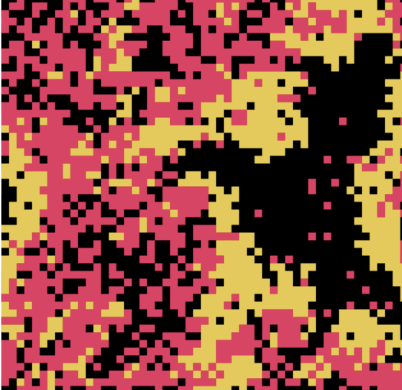
\includegraphics[width=0.3\textwidth,height=\textheight]{Modellering/figuren/lv_todo.png}

}

\caption{Deze moet nog gemaakt worden. Net als bij de Australie-vraag
wil ik een legenda en uitleg maken erbij.}

\end{figure}

In Hoofdstuk~\ref{sec-exp} hebben we een miniatuur Australië bestudeert
waarin konijnen zich konden verspreiden. Hierbij zagen we enkele
verschillen tussen het wiskundige model (de differentievergelijking /
ODEs) en het ruimtelijke model. Ook in de vorige vraag zagen we dat een
gemengd SIR-systeem en een ongemengd SIR-systeem enorm verschillen! We
gaan nu bestuderen of Lotka-Volterra in een ruimtelijk model ook
belangrijke verschillen heeft.

Wederom delen we de ruimte op in verschillende types hokjes: lege hokjes
(zwart), prooidierhokjes (geel), en predatorhokjes (rood). (zie FIGUUR
TODO). Prooidieren kunnen een leeg, nabijgelegen hokje in een
prooidierhokje veranderen (dit stelt geboorte voor). Als er geen leeg
hokje beschikbaar is, kan de prooi niet reproduceren. De predator kan
alleen reproduceren als er een nabijgelegen prooihokje is, en verandert
deze dan in een predatorhokje. Beide types individuen sterven met 4\%
kans, waardoor het hokje weer leeg wordt.

Net als bij de konijnen in Australië, hoeven we geen extra
dichtheidseffect in te bouwen omdat deze automatisch bestaat: het aantal
hokjes is eindig.

In dit ``toy-model'' wordt predatie versimpeld tot 1 prooihokje in 1
predatorhokje veranderen.

\begin{enumerate}
\def\labelenumi{\alph{enumi}.}
\tightlist
\item
  Wat zegt dit over de parameter \(c\) zoals je die in dit hoofdstuk
  hebt leren kennen? \emph{die is 1}
\end{enumerate}

Bekijk de simulatie en de grafieken.

\begin{enumerate}
\def\labelenumi{\alph{enumi}.}
\setcounter{enumi}{1}
\item
  Correspondeert dit resultaat met de inwaardse spiraal die we in de
  faseruimte van dit hoofdstuk gezien hebben? \emph{ja}
\item
  Bij hoeveel prooi/predator stabiliseert het systeem ongeveer? Kun je
  voorbeelden bedenken van predator-prooi systemen die een dergelijke
  verhouding hebben? \emph{\textasciitilde2300 prooi,
  \textasciitilde11000 predator (dus meer predatoren dan prooi). Een
  goede student zal wellicht begrijpen dat dit bij konijnen en vossen
  zeker niet het geval is. Het komt vooral wel voor bij parasieten en
  virussen (ook een soort `predator'!), en bij wolven en andere
  predatoren die in groepen op groot wild jagen}
\end{enumerate}

Gebruik de knoppen onderaan de simulatie om de populatie te mengen, en
wacht tot deze nieuwe situatie in evenwicht is. Start de simulatie ook
een keer opnieuw onder gemengde onstandigheden.

\begin{enumerate}
\def\labelenumi{\alph{enumi}.}
\setcounter{enumi}{3}
\item
  Bij welke populatiegroottes stabilseert het systeem nu? \emph{je
  krijgt vooral veel meer predatoren erbij}
\item
  Een van de populaties lijkt veel meer gebaat bij een gemengd systeem
  dan de ander. Waarom is dat denk je? \emph{predator kan makkelijker
  prooi vangen. prooi kan ook makkelijker geboren worden, maar zoals we
  in de ODEs hebben gezien gaat die verrijking allemaal OOK in de
  predator zitten!}
\end{enumerate}

Ga terug naar de ongemengde simulatie. Wacht tot de populatie is
gestabiliseerd, en gebruik daarna de knoppen om de death rate van de
predator te halveren.

\begin{enumerate}
\def\labelenumi{\alph{enumi}.}
\setcounter{enumi}{5}
\item
  Omschrijf wat er gebeurt (halveer zo nodig de death rate van de
  predatoren nog eens). \emph{je ziet niet per se meer predatoren, maar
  meer oscillsaties. Je ziet ook dat het `lijntje prooien' steeds dunner
  wordt }
\item
  Wat gebeurt er als de death rate van de predator heel laag is
  (bijvoorbeeld 0.001)? Denk je dat dit ook in de ODEs zou gebeuren?
  \emph{dit is een aardig advanced vraag voor eerstejaars, dus het
  antwoord moet goed zijn want weinig zullen het meteen helemaal
  doorzien. de prooi kan helemaal uitsterven door de predator, waarna de
  predator ook dood gaat. dit zou in de ODEs niet gebeuren, want je kan
  de assen alleen maar langzaam naderen (het zijn nullclines, dus hoe
  dichter bij je bent, hoe langzamer je er op af gaat)}
\end{enumerate}

\end{exercise}

\begin{exercise}[Virus-uitbraak]\protect\hypertarget{exr-virusuitbraak}{}\label{exr-virusuitbraak}

Als een nieuw virus ontstaat, kan deze zich vroeg in de epidemie vaak
enorm hard uitbreiden: veel individuen zijn nog niet resistent. Over de
tijd zullen individuen echter resistent worden. Zodoende hebben we te
maken met drie type individuen: vatbare individuen (\emph{susceptibles},
\(S\)), geinfecteerde individuen (\emph{infected}, \(I\)), en resistente
individuen (\emph{recovered}, \(R\)). De totale populatiegrootte
(\(S\)+\(I\)+\(R\)), kunnen we \(N\) noemen. Nu kunnen we een systeem
van drie ODEs opstellen:

\begin{align}
N &= S+I+R\\
\mathchoice{\frac{\mathrm{d}S}
{\mathrm{d}t}}{\mathrm{d}S/\mathrm{d}t}
{\mathrm{d}S/\mathrm{d}t}
{\mathrm{d}S/\mathrm{d}t} &= b(1-\frac{N}{K})S - dS - \beta S I \\
\mathchoice{\frac{\mathrm{d}I}
{\mathrm{d}t}}{\mathrm{d}I/\mathrm{d}t}
{\mathrm{d}I/\mathrm{d}t}
{\mathrm{d}I/\mathrm{d}t} &= \beta SI - (d+\delta)I - rI \\
\mathchoice{\frac{\mathrm{d}R}
{\mathrm{d}t}}{\mathrm{d}R/\mathrm{d}t}
{\mathrm{d}R/\mathrm{d}t}
{\mathrm{d}R/\mathrm{d}t} &= rI - dR
\end{align}

Bekijk de vergelijkingen hierboven.

\begin{enumerate}
\def\labelenumi{\alph{enumi}.}
\item
  Planten alle individuen (susceptible, infected, recovered) zich voort?
  \emph{ANTWOORD: nee alleen S}
\item
  In welke eenheden wordt de \(\delta\) parameter uitgedrukt? Wat is de
  biologische interpretatie van deze parameter? \emph{deltaI = I/tijd
  dus delta = 1/tijd, dus `per tijdseenheid'. De parameter geeft een
  hogere death rate aan geinfecteerde individuen}
\end{enumerate}

Aangenomen dat de parameters positief zijn (en dat de infectie zich kan
verspreiden), kunnen we een oplossing met de computer doorrekenen. Omdat
dit 3 ODEs zijn, geeft dit ook 3 grafiekjes (zie Figuur hieronder).

\begin{enumerate}
\def\labelenumi{\alph{enumi}.}
\setcounter{enumi}{2}
\tightlist
\item
  Waarom is de eerste piek van de rode lijn het hoogst?
\end{enumerate}

\begin{Shaded}
\begin{Highlighting}[]
\CommentTok{\#| code{-}fold: true}

\CommentTok{\#| eval: true}

\CommentTok{\#| fig.width: 6}

\CommentTok{\#| fig.height: 3}

\FunctionTok{par}\NormalTok{(}\AttributeTok{mar=}\FunctionTok{c}\NormalTok{(}\DecValTok{4}\NormalTok{,}\DecValTok{4}\NormalTok{,}\DecValTok{0}\NormalTok{,}\DecValTok{2}\NormalTok{))}

\NormalTok{model }\OtherTok{\textless{}{-}} \ControlFlowTok{function}\NormalTok{(t, state, parms)\{}

  \FunctionTok{with}\NormalTok{(}\FunctionTok{as.list}\NormalTok{(}\FunctionTok{c}\NormalTok{(state,parms)),\{}

\NormalTok{    N }\OtherTok{\textless{}{-}}\NormalTok{ S}\SpecialCharTok{+}\NormalTok{I}\SpecialCharTok{+}\NormalTok{R}

\NormalTok{    dS }\OtherTok{\textless{}{-}}\NormalTok{ b}\SpecialCharTok{*}\NormalTok{(}\DecValTok{1}\SpecialCharTok{{-}}\NormalTok{N}\SpecialCharTok{/}\NormalTok{K)}\SpecialCharTok{*}\NormalTok{S }\SpecialCharTok{{-}}\NormalTok{ d}\SpecialCharTok{*}\NormalTok{S }\SpecialCharTok{{-}}\NormalTok{ beta}\SpecialCharTok{*}\NormalTok{S}\SpecialCharTok{*}\NormalTok{I}

\NormalTok{    dI }\OtherTok{\textless{}{-}}\NormalTok{ beta}\SpecialCharTok{*}\NormalTok{S}\SpecialCharTok{*}\NormalTok{I }\SpecialCharTok{{-}}\NormalTok{ (d}\SpecialCharTok{+}\NormalTok{delta)}\SpecialCharTok{*}\NormalTok{I }\SpecialCharTok{{-}}\NormalTok{ r}\SpecialCharTok{*}\NormalTok{I}

\NormalTok{    dR }\OtherTok{\textless{}{-}}\NormalTok{ r}\SpecialCharTok{*}\NormalTok{I }\SpecialCharTok{{-}}\NormalTok{ d}\SpecialCharTok{*}\NormalTok{R}

    \FunctionTok{return}\NormalTok{(}\FunctionTok{list}\NormalTok{(}\FunctionTok{c}\NormalTok{(dS,dI,dR)))}

\NormalTok{  \})}

\NormalTok{\}}

\NormalTok{colors[}\DecValTok{1}\NormalTok{] }\OtherTok{=} \StringTok{"\#4E1681"}

\NormalTok{colors[}\DecValTok{2}\NormalTok{] }\OtherTok{=} \StringTok{"\#F05D5D"}

\NormalTok{colors[}\DecValTok{3}\NormalTok{] }\OtherTok{=} \StringTok{"\#e2d5cb"}

\NormalTok{p }\OtherTok{\textless{}{-}} \FunctionTok{c}\NormalTok{(}\AttributeTok{b=}\FloatTok{0.7}\NormalTok{,}\AttributeTok{beta=}\FloatTok{0.3}\NormalTok{,}\AttributeTok{r=}\FloatTok{0.1}\NormalTok{,}\AttributeTok{d=}\FloatTok{0.1}\NormalTok{,}\AttributeTok{delta=}\FloatTok{0.1}\NormalTok{,}\AttributeTok{K=}\DecValTok{4}\NormalTok{)}

\NormalTok{s }\OtherTok{\textless{}{-}} \FunctionTok{c}\NormalTok{(}\AttributeTok{S=}\FloatTok{3.5}\NormalTok{,}\AttributeTok{I=}\FloatTok{0.001}\NormalTok{,}\AttributeTok{R=}\FloatTok{0.0}\NormalTok{)}

\NormalTok{plot }\OtherTok{\textless{}{-}} \FunctionTok{run}\NormalTok{(}\AttributeTok{tmax=}\DecValTok{100}\NormalTok{,}\AttributeTok{ylab=}\StringTok{"Dichtheden"}\NormalTok{,}\AttributeTok{xlab=}\StringTok{"Tijd"}\NormalTok{)}
\end{Highlighting}
\end{Shaded}

\begin{figure}[H]

{\centering 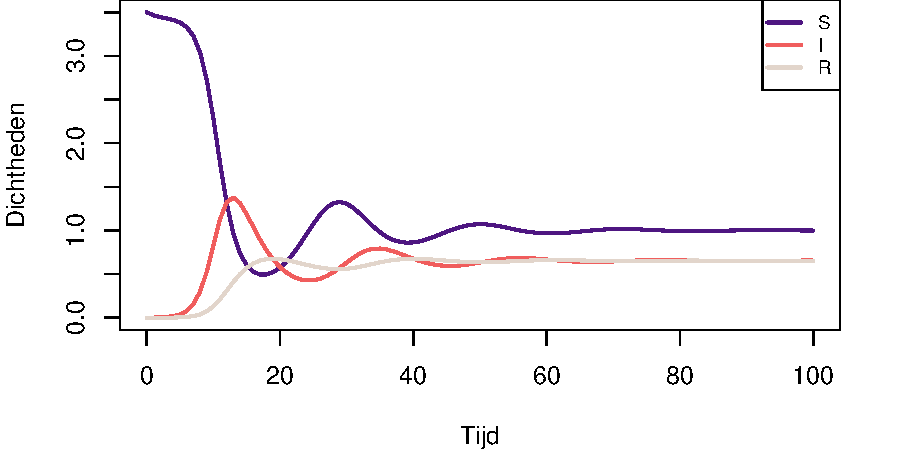
\includegraphics{Modellering/ecoevo_meerdere_files/figure-pdf/unnamed-chunk-10-1.pdf}

}

\end{figure}

Tijdens de Covid-19 pandemie hebben we gezien dat twee maatregelen zeer
effectief waren: 1.) \emph{social distancing} en 2)
\emph{contactbeperkingen}. Hieronder zie je een interactieve simulatie
van bovenstaande interacties in een ruimtelijk model. Met de `mengen'
optie worden na elke tijdstap alle individuen volledig gehusseld.

\begin{enumerate}
\def\labelenumi{\alph{enumi}.}
\setcounter{enumi}{3}
\item
  Controlleer of onder gemengde omstandigheden dit model zich zoals het
  ODE model gedraagt. \emph{ja zeer vergelijkbaar}
\item
  Is het effect in deze simulatie meer vergelijkbaar met \emph{social
  distancing} of met \emph{contactbeperkingen}? \emph{contactbeperking,
  de pixels dezelfde afstand van elkaar houden}
\end{enumerate}

\begin{enumerate}
\def\labelenumi{\alph{enumi}.}
\setcounter{enumi}{5}
\tightlist
\item
  Maak de \(\beta\)-parameters van het virus hoger (bijvoorbeeld 0.1,
  maar je kan ook andere waarden proberen). Beschrijf in je eigen
  woorden wat er gebeurt voor zowel gemengde als ongemende
  omstandigheden. \emph{In het ongemengde systeem zie je dat het virus
  uitsterft, omdat het zich te snel verspreidt en daardoor alle vatbare
  individuen op consumeert. Kleine populaties vatbare individuen blijven
  echter achter en groeien uiteindelijk weer terug; maar het virus is al
  weg! In het gemengde systeem daarentegen sterft de gehele populatie
  uit: het agressieve virus kan altijd een nieuw slachtoffer vinden,
  waardoor er geen overlevenden zijn.}
\end{enumerate}

\end{exercise}

\begin{exercise}[Een 3D
systeem]\protect\hypertarget{exr-3dsysteem}{}\label{exr-3dsysteem}

\begin{figure}

{\centering 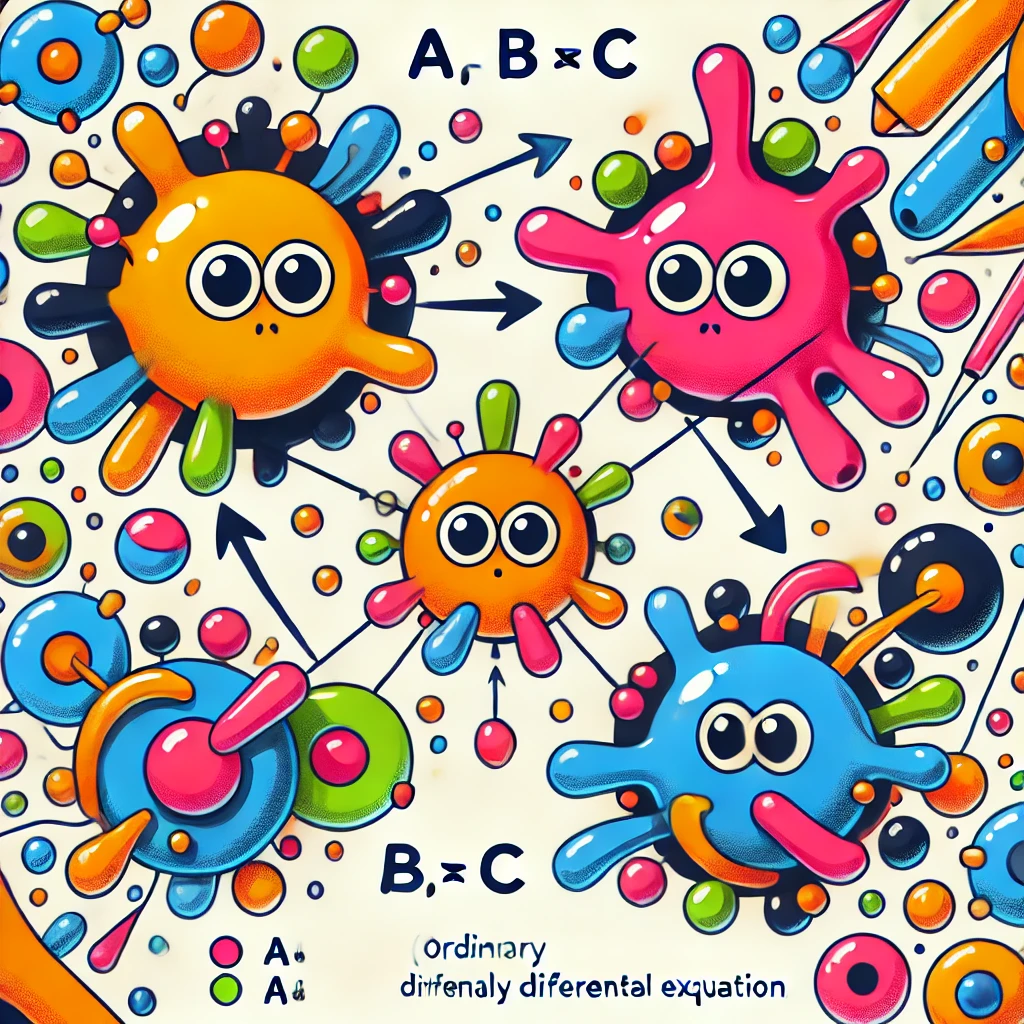
\includegraphics[width=0.6\textwidth,height=\textheight]{Modellering/figuren/abc.png}

}

\end{figure}

Bekijk het volgende 3D ODE systeem van een voedselketen (B eet A, C eet
B):

\begin{align*}
\mathchoice{\frac{\mathrm{d}A}
{\mathrm{d}t}}{\mathrm{d}A/\mathrm{d}t}
{\mathrm{d}A/\mathrm{d}t}
{\mathrm{d}A/\mathrm{d}t} &= rA(1-A/k)-cAB \\
\mathchoice{\frac{\mathrm{d}B}
{\mathrm{d}t}}{\mathrm{d}B/\mathrm{d}t}
{\mathrm{d}B/\mathrm{d}t}
{\mathrm{d}B/\mathrm{d}t} &= cAB - dB - eBC \\
\mathchoice{\frac{\mathrm{d}C}
{\mathrm{d}t}}{\mathrm{d}C/\mathrm{d}t}
{\mathrm{d}C/\mathrm{d}t}
{\mathrm{d}C/\mathrm{d}t} &= eBC - fC
\end{align*}

\begin{enumerate}
\def\labelenumi{\alph{enumi}.}
\item
  Wat betekent het dat de term \(cAB\) in precies dezelfde vorm
  terugkomt in \(\mathchoice{\frac{\mathrm{d}A}
  {\mathrm{d}t}}{\mathrm{d}A/\mathrm{d}t}
  {\mathrm{d}A/\mathrm{d}t}
  {\mathrm{d}A/\mathrm{d}t}\) en \(\mathchoice{\frac{\mathrm{d}B}
  {\mathrm{d}t}}{\mathrm{d}B/\mathrm{d}t}
  {\mathrm{d}B/\mathrm{d}t}
  {\mathrm{d}B/\mathrm{d}t}\)? \emph{dat biomassa conversie perfect is:
  elke 1 A die opgegeten wordt levert 1 B op. Dit geldt overigens ook
  voor conversie van B naar C.}
\item
  Ga ervan uit dat alle drie de populaties in evenwicht aanwezig zijn.
  Bepaal voor deze situatie de hoeveelheid \(B\) in evenwicht (hint:
  denk eerst even goed na, dit is namelijk heel makkelijk!)
\end{enumerate}

\emph{als allemaal aanwezig zijn is C dus ook aanwezig (dus niet 0). Dit
betekend dat we B kunnen vinden uit dC/dt dus 0, door eerst te delen
door C (C is niet 0, dus dat mag), en dan voor B op te lossen: B = f/e}

\end{exercise}

\hypertarget{terminologie-5}{%
\section{Terminologie}\label{terminologie-5}}

TODO

\hypertarget{odes-modelleren-met-r}{%
\chapter{ODEs modelleren met R}\label{odes-modelleren-met-r}}

In Hoofdstuk~\ref{sec-meerdere} hebben we een heel beroemd model uit de
biologie geanalyseerd: het \emph{Lotka-Volterra predator-prooi model}.
Dit model gaat natuurlijk niet specifiek over konijnen en vossen, maar
zou op allerlei systemen toegepast kunnen worden: bacteriofagen die
bacteriën infecteren, protozoa die bacteriën eten, lieveheersbeestjes
die bladluizen eten, vleermuizen die motjes eten, \emph{etc.} Daarnaast
kun je met kleine aanpassingen ook meer subtiele interacties tussen
soorten onderzoeken (zoals intra- en inter-specifieke competitie, later
in dit hoofdstuk). Zodoende is het Lotka-Volterra model uitgegroeid tot
één van de meest veelzijdige modellen in de biologie, waarmee
voorspellingen gedaan kunnen worden over welke soorten wel/niet kunnen
samenleven.

\begin{figure}

{\centering 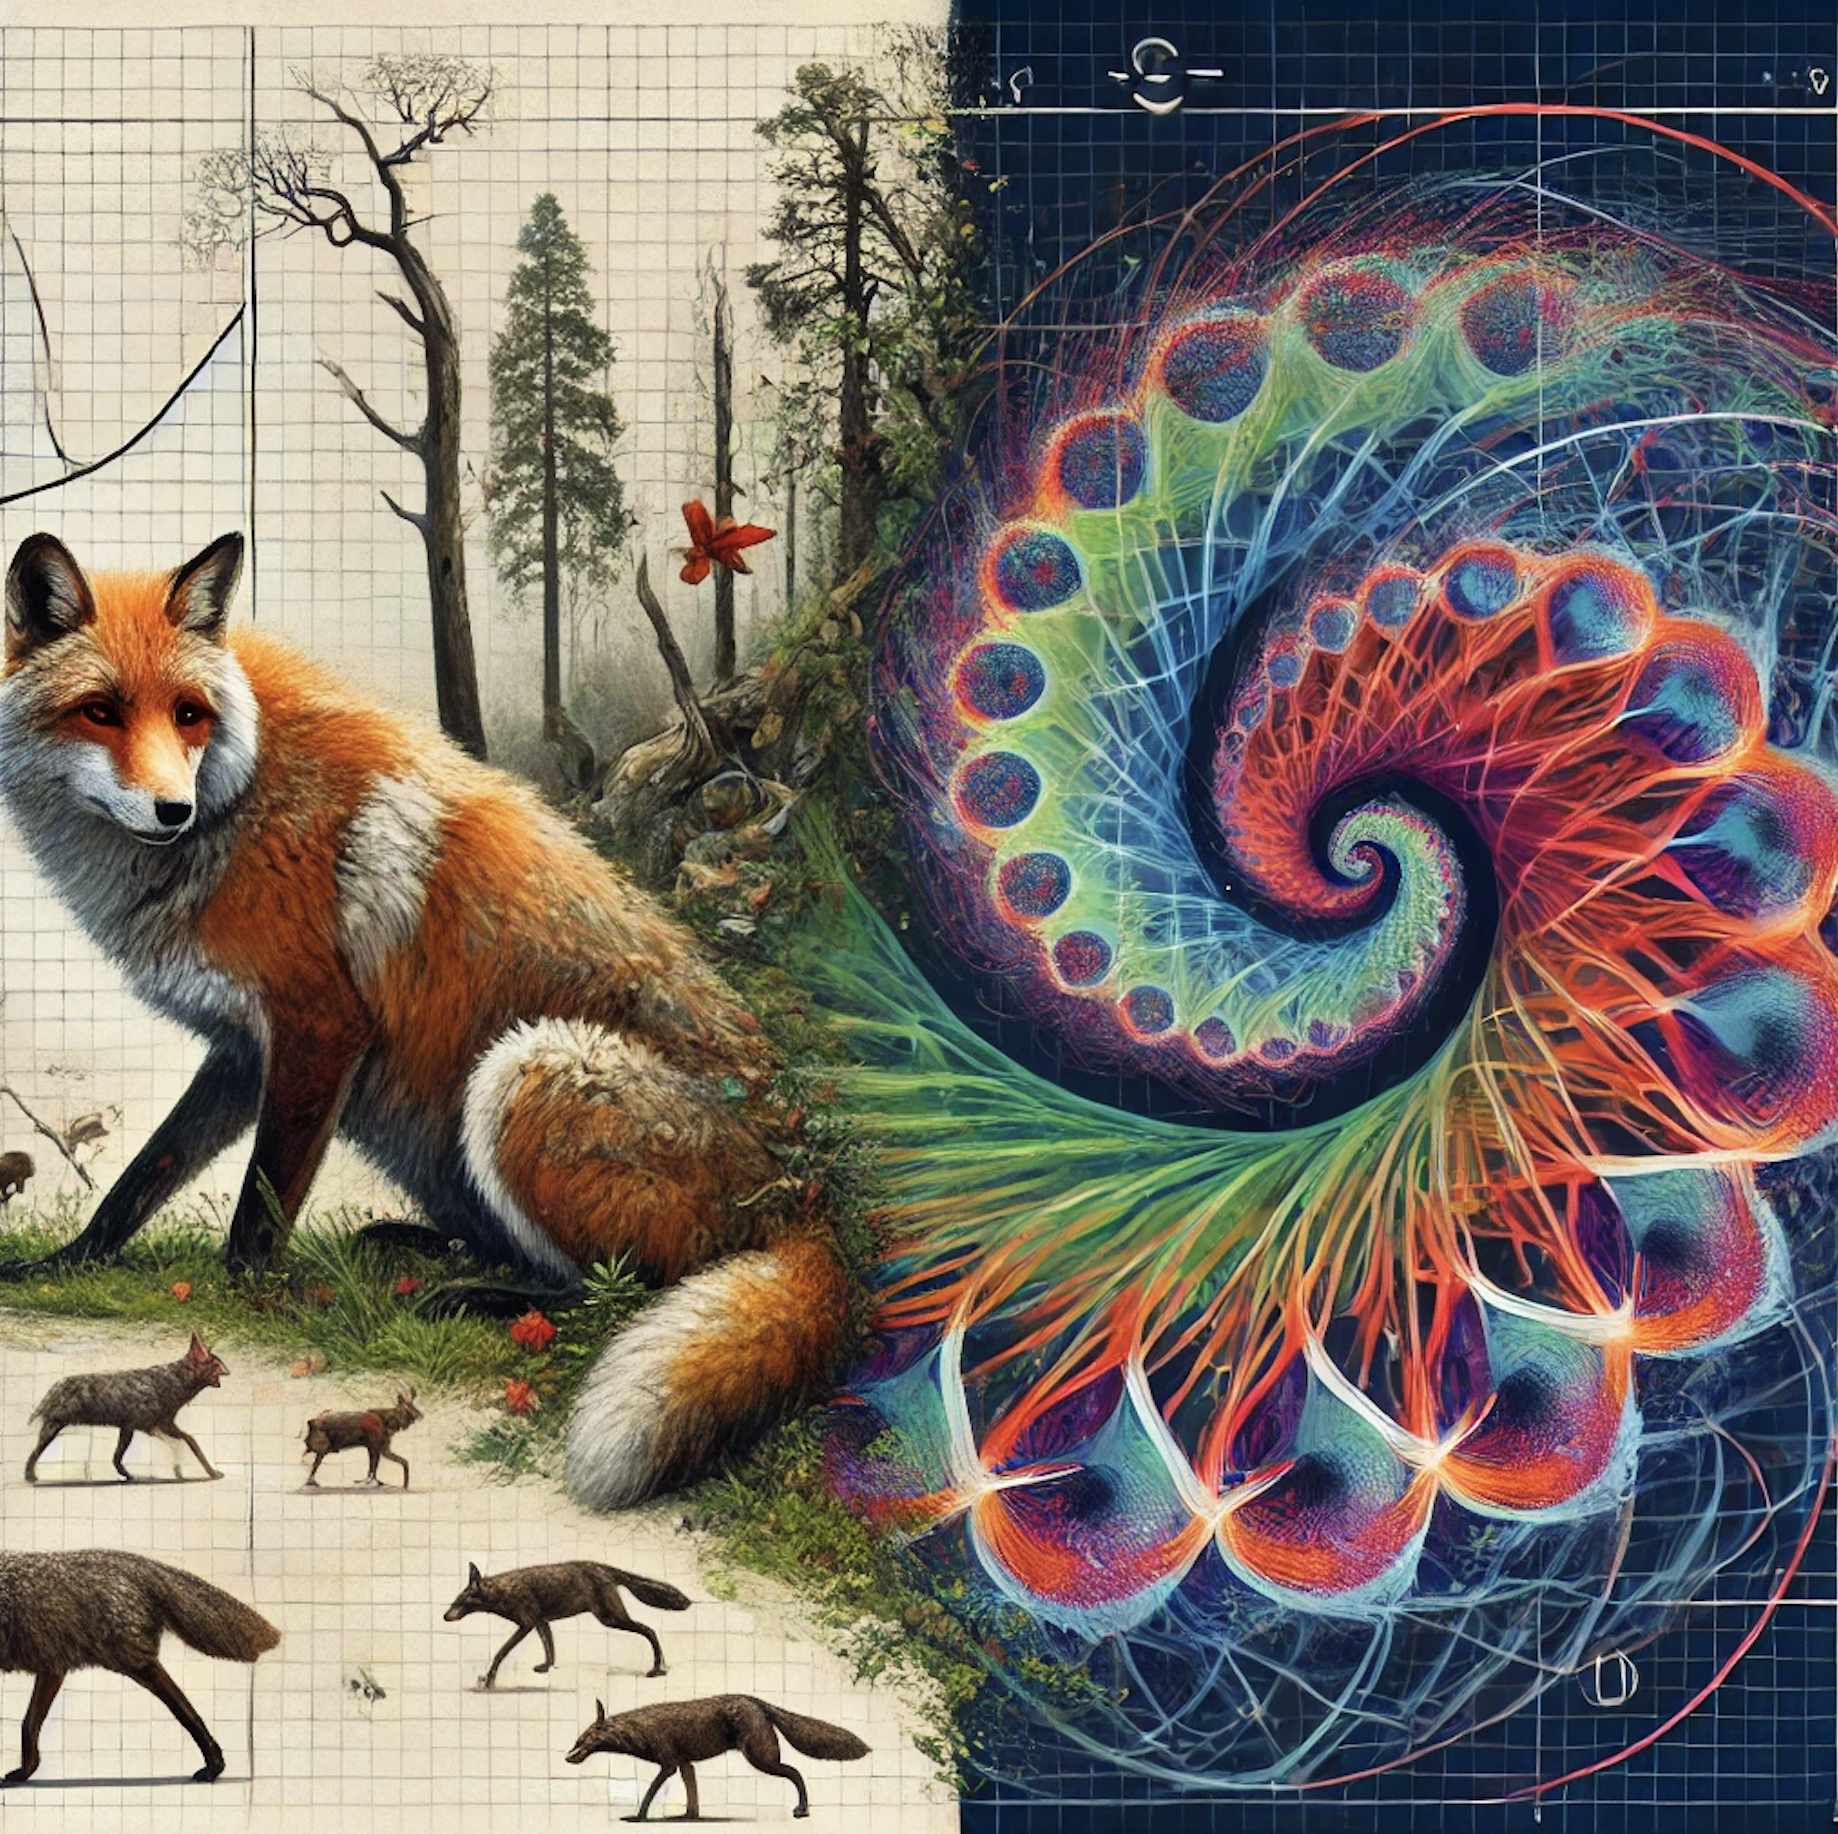
\includegraphics[width=0.8\textwidth,height=\textheight]{Modellering/figuren/lv_spiral_ai.png}

}

\caption{Afbeelding gegenereerd met ChatGPT4-o}

\end{figure}

\hypertarget{leerdoelen-6}{%
\section{Leerdoelen}\label{leerdoelen-6}}

De leerdoelen voor dit hoofdstuk zijn:

\begin{itemize}
\tightlist
\item
  Begrijpen hoe een simpel model (zoals het Lotka-Volterra model) kan
  worden uitgebreid door extra details in te voegen (bijvoorbeeld een
  predator die verzadigd)
\item
  Een Hill-functie herkennen, en de kenmerken kunnen benoemen (initiële
  helling, half-waarde, maximum)
\item
  R kunnen gebruiken om faseruimtes met nullclines en trajectories te
  tekenen, en de daarbij horende oplossingen
\end{itemize}

\hypertarget{de-verzadigde-predator}{%
\section{De verzadigde predator}\label{de-verzadigde-predator}}

We hebben gezien hoe met behulp van faseruimtes het best eenvoudig kan
zijn om inzicht in een biologisch proces te vergaten. Maar de eenvoud
van deze eerdere analyses is deels te verklaren door de eenvoud van het
model dat we hebben gebruikt. In ons eerdere Lotka-Volterra model namen
we bijvoorbeeld aan dat predatie lineair proportioneel is aan de
dichtheden predator en prooi door gebruik te maken van de predatieterm
\(aRN\). Dit betekend dat per predator (ookwel: \emph{per capita}) in
totaal \(aR\) prooi gegeten kan worden (nogmaals, ``per'' kun je lezen
als ``gedeeld door'', dus \(\frac{aRN}{N} = aR\)). Bij oneindig hoge
prooi dichtheden, kan er dus ook oneindig veel gegeten worden. In het
echt zal een predator eigenlijk een tijd bezig zijn met het verwerken en
verteren van de prooi. Zodoende zal de predatie-term bij hele hoge
prooi-dichtheden eigenlijk moeten verzadigen. Om dit te verwerken,
zouden we de predatie-term aan kunnen passen:

\begin{align*}
\frac{\mathrm{d}\color{blue}R}{\mathrm{d}t} &= \underbrace{b(1-\frac{\color{blue}R}{K})\color{blue}R}_{\text{geboorte prooi}} - \underbrace{d\color{blue}R}_{\text{sterfte prooi}} - \underbrace{\frac{\color{black}a\color{blue}R\color{orange}N}{h+\color{blue}R\color{black}}}_{\text{nieuwe predatieterm}}\\
\color{black}\frac{\mathrm{d}\color{orange}N}{\mathrm{d}t} &\color{black}= \underbrace{\frac{\color{black}a\color{blue}R\color{orange}N}{h+\color{blue}R\color{black}}}_{\text{geboorte predator}} - \underbrace{\delta \color{orange}N}_{\text{sterfte predator}}
\end{align*}

Wat is met deze nieuwe predator-term de \emph{per capita} predatie? Dat
wil zeggen: hoeveel prooi kan een enkele predator per tijdseenheid
opeten? Hiervoor delen we wederom de predatie-term door \(N\), waardoor
we functie \(\frac{aR}{h+R}\) krijgen. Om een beeld van deze functie te
krijgen, is het handig om deze even te schetsen.

\hypertarget{hill-functies}{%
\section{Hill-functies}\label{hill-functies}}

Laten we eerst even naar de noemer te kijken, en vooral naarde balans
tussen \(h\) en \(R\). Als \(R\) heel klein is, heeft \(h\) de overhand
in de noemer, waardoor \(R\) verwaarloosbaar is. Dus voor kleine \(R\)
nadert de functie \(\frac{aR}{h}\), wat een lineaire toename is. Dus
voor kleine prooi-dichtheden, neemt predatie lineair toe met de
prooi-dichtheid, net zoals in het eerdere model. Maar als \(R\) alsmaar
groter wordt, wordt \(h\) juist verwaarloosbaar ten opzichte van \(R\).
Daarom nadert deze functie bij hoge \(R\) de waarde
\(\frac{aR}{R} = a\). Dus: zelfs bij hele hoge prooidichtheiden kan een
enkele predator per tijdseenheid (bijv. per dag) hoogstens \(a\) prooi
eten. Tussen deze twee extreme waarden zit nog een laatste bijzondere
punt: het punt waar \(R\) precies gelijk is aan \(h\). Op dit punt is de
functie gelijk aan \(\frac{aR}{R+R}=\frac{aR}{2R}=\frac{a}{2}\). De
parameter \(h\) geeft dus de prooi-dichtheid waar de predatieterm
half-maximaal is. Nu kunnen we de functie schetsen, zoals weergegeven in
Figuur~\ref{fig-predatieterm-1}.

Functies van deze vorm worden ``Hill-functies'' genoemd (vernoemd naar
Archibald Hill, niet naar het feit dat het een soort heuveltje is). Met
een kleine aanpassing aan deze Hill-functie (\(\frac{aR^2}{h^2+R^2}\)),
kun je deze response ook sigmoide laten verlopen
(Figuur~\ref{fig-predatieterm-2}).

\begin{Shaded}
\begin{Highlighting}[]
\NormalTok{a}\OtherTok{=}\DecValTok{1}
\NormalTok{h}\OtherTok{=}\DecValTok{1}

\NormalTok{func }\OtherTok{\textless{}{-}} \ControlFlowTok{function}\NormalTok{(x)\{}
  \FunctionTok{return}\NormalTok{(a}\SpecialCharTok{*}\NormalTok{x}\SpecialCharTok{/}\NormalTok{(x}\SpecialCharTok{+}\NormalTok{h))}
\NormalTok{\}}

\FunctionTok{curve}\NormalTok{(func,}\DecValTok{0}\NormalTok{,}\DecValTok{8}\NormalTok{,}\AttributeTok{lwd=}\DecValTok{2}\NormalTok{,}\AttributeTok{ylim=}\FunctionTok{c}\NormalTok{(}\DecValTok{0}\NormalTok{,}\FloatTok{1.}\NormalTok{), }\AttributeTok{xaxt=}\StringTok{"n"}\NormalTok{, }\AttributeTok{yaxt=}\StringTok{"n"}\NormalTok{,}
      \AttributeTok{ylab=}\StringTok{"Predatie"}\NormalTok{,}\AttributeTok{xlab=}\StringTok{"Hoeveelheid prooi (R)"}\NormalTok{,}\AttributeTok{col=}\StringTok{"seagreen"}\NormalTok{,}
      \AttributeTok{main=}\StringTok{"Hill{-}functie (Type 2)"}\NormalTok{)}

\FunctionTok{axis}\NormalTok{(}\DecValTok{1}\NormalTok{, }\AttributeTok{labels =} \ConstantTok{FALSE}\NormalTok{) }\CommentTok{\# x{-}axis}
\FunctionTok{axis}\NormalTok{(}\DecValTok{2}\NormalTok{, }\AttributeTok{labels =} \ConstantTok{FALSE}\NormalTok{) }\CommentTok{\# x{-}axis}
\FunctionTok{abline}\NormalTok{(}\AttributeTok{h=}\NormalTok{a,}\AttributeTok{lty=}\DecValTok{2}\NormalTok{,}\AttributeTok{col=}\StringTok{"grey"}\NormalTok{)}
\FunctionTok{abline}\NormalTok{(}\AttributeTok{v=}\NormalTok{h,}\AttributeTok{lty=}\DecValTok{2}\NormalTok{,}\AttributeTok{col=}\StringTok{"grey"}\NormalTok{)}
\FunctionTok{mtext}\NormalTok{(}\StringTok{"h"}\NormalTok{,}\AttributeTok{side=}\DecValTok{1}\NormalTok{,}\AttributeTok{at=}\NormalTok{h,}\AttributeTok{line=}\FloatTok{0.7}\NormalTok{)}
\FunctionTok{mtext}\NormalTok{(}\StringTok{"0"}\NormalTok{,}\AttributeTok{side=}\DecValTok{1}\NormalTok{,}\AttributeTok{line=}\FloatTok{0.5}\NormalTok{,}\AttributeTok{at=}\DecValTok{0}\NormalTok{)}
\FunctionTok{mtext}\NormalTok{(}\StringTok{"0"}\NormalTok{,}\AttributeTok{side=}\DecValTok{2}\NormalTok{,}\AttributeTok{line=}\FloatTok{0.5}\NormalTok{,}\AttributeTok{at=}\DecValTok{0}\NormalTok{)}
\FunctionTok{text}\NormalTok{(}\SpecialCharTok{{-}}\FloatTok{1.5}\NormalTok{,}\DecValTok{1}\NormalTok{,}\StringTok{"a"}\NormalTok{,}\AttributeTok{xpd=}\ConstantTok{NA}\NormalTok{)}

\NormalTok{func }\OtherTok{\textless{}{-}} \ControlFlowTok{function}\NormalTok{(x)\{}
  \FunctionTok{return}\NormalTok{(a}\SpecialCharTok{*}\NormalTok{x}\SpecialCharTok{\^{}}\DecValTok{2}\SpecialCharTok{/}\NormalTok{(x}\SpecialCharTok{\^{}}\DecValTok{2}\SpecialCharTok{+}\NormalTok{h}\SpecialCharTok{\^{}}\DecValTok{2}\NormalTok{))}
\NormalTok{\}}

\FunctionTok{curve}\NormalTok{(func,}\DecValTok{0}\NormalTok{,}\DecValTok{3}\NormalTok{,}\AttributeTok{lwd=}\DecValTok{2}\NormalTok{,}\AttributeTok{ylim=}\FunctionTok{c}\NormalTok{(}\DecValTok{0}\NormalTok{,}\FloatTok{1.}\NormalTok{), }\AttributeTok{xaxt=}\StringTok{"n"}\NormalTok{, }\AttributeTok{yaxt=}\StringTok{"n"}\NormalTok{,}
      \AttributeTok{ylab=}\StringTok{"Predatie"}\NormalTok{,}\AttributeTok{xlab=}\StringTok{"Hoeveelheid prooi (R)"}\NormalTok{,}\AttributeTok{col=}\StringTok{"seagreen"}\NormalTok{,}
      \AttributeTok{main=}\StringTok{"Hill{-}functie (Type 3)"}\NormalTok{)}

\FunctionTok{axis}\NormalTok{(}\DecValTok{1}\NormalTok{, }\AttributeTok{labels =} \ConstantTok{FALSE}\NormalTok{) }\CommentTok{\# x{-}axis}
\FunctionTok{axis}\NormalTok{(}\DecValTok{2}\NormalTok{, }\AttributeTok{labels =} \ConstantTok{FALSE}\NormalTok{) }\CommentTok{\# x{-}axis}
\FunctionTok{abline}\NormalTok{(}\AttributeTok{h=}\NormalTok{a,}\AttributeTok{lty=}\DecValTok{2}\NormalTok{,}\AttributeTok{col=}\StringTok{"grey"}\NormalTok{)}
\FunctionTok{abline}\NormalTok{(}\AttributeTok{v=}\NormalTok{h,}\AttributeTok{lty=}\DecValTok{2}\NormalTok{,}\AttributeTok{col=}\StringTok{"grey"}\NormalTok{)}
\FunctionTok{mtext}\NormalTok{(}\StringTok{"h"}\NormalTok{,}\AttributeTok{side=}\DecValTok{1}\NormalTok{,}\AttributeTok{at=}\NormalTok{h,}\AttributeTok{line=}\FloatTok{0.7}\NormalTok{)}
\FunctionTok{mtext}\NormalTok{(}\StringTok{"0"}\NormalTok{,}\AttributeTok{side=}\DecValTok{1}\NormalTok{,}\AttributeTok{line=}\FloatTok{0.5}\NormalTok{,}\AttributeTok{at=}\DecValTok{0}\NormalTok{)}
\FunctionTok{mtext}\NormalTok{(}\StringTok{"0"}\NormalTok{,}\AttributeTok{side=}\DecValTok{2}\NormalTok{,}\AttributeTok{line=}\FloatTok{0.5}\NormalTok{,}\AttributeTok{at=}\DecValTok{0}\NormalTok{)}
\FunctionTok{text}\NormalTok{(}\SpecialCharTok{{-}}\FloatTok{0.5}\NormalTok{,}\DecValTok{1}\NormalTok{,}\StringTok{"a"}\NormalTok{,}\AttributeTok{xpd=}\ConstantTok{NA}\NormalTok{)}
\end{Highlighting}
\end{Shaded}

\begin{figure}

\begin{minipage}[t]{0.50\linewidth}

{\centering 

\raisebox{-\height}{

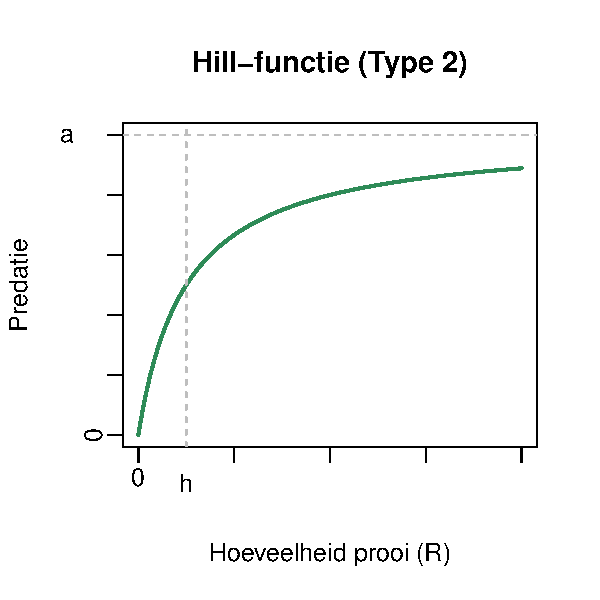
\includegraphics{Modellering/ecoevo_grindbif_files/figure-pdf/fig-predatieterm-1.pdf}

}

}

\subcaption{\label{fig-predatieterm-1}\textbf{?(caption)}}
\end{minipage}%
%
\begin{minipage}[t]{0.50\linewidth}

{\centering 

\raisebox{-\height}{

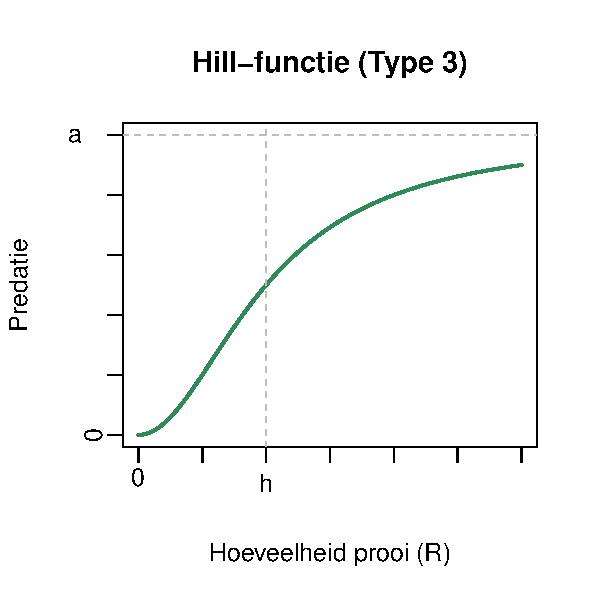
\includegraphics{Modellering/ecoevo_grindbif_files/figure-pdf/fig-predatieterm-2.pdf}

}

}

\subcaption{\label{fig-predatieterm-2}\textbf{?(caption)}}
\end{minipage}%

\caption{\label{fig-predatieterm}\textbf{?(caption)}}

\end{figure}

\begin{exercise}[Hill-functies]\protect\hypertarget{exr-hillfuncties}{}\label{exr-hillfuncties}

De bovengenoemde Hill-functies zijn zeer veelzijdig, en met kleine
aanpassingen kun je de vorm goed aanpassen. Vaak willen we kunnen
wisselen tussen geen interactie (0) en volledige interactie (1), of geen
genexpressie (0) en volledige genexpressie (1), \emph{etc.}. Zodoende
kunnen we de parameter \(a\) op 1 veronderstellen, en deze dus weglaten.
Neem de onderstaande code over in R:

\begin{Shaded}
\begin{Highlighting}[]
\NormalTok{h}\OtherTok{=}\DecValTok{1}
\NormalTok{n}\OtherTok{=}\DecValTok{2}

\NormalTok{func }\OtherTok{\textless{}{-}} \ControlFlowTok{function}\NormalTok{(x)\{}
  \FunctionTok{return}\NormalTok{(x}\SpecialCharTok{\^{}}\NormalTok{n}\SpecialCharTok{/}\NormalTok{(x}\SpecialCharTok{\^{}}\NormalTok{n}\SpecialCharTok{+}\NormalTok{h}\SpecialCharTok{\^{}}\NormalTok{n))}
\NormalTok{\}}

\FunctionTok{curve}\NormalTok{(func,}\DecValTok{0}\NormalTok{,}\DecValTok{3}\NormalTok{,}\AttributeTok{lwd=}\FloatTok{2.5}\NormalTok{,}\AttributeTok{ylim=}\FunctionTok{c}\NormalTok{(}\DecValTok{0}\NormalTok{,}\FloatTok{1.}\NormalTok{), }
      \AttributeTok{ylab=}\StringTok{"f(x)"}\NormalTok{,}\AttributeTok{xlab=}\StringTok{"x"}\NormalTok{,}\AttributeTok{col=}\StringTok{"seagreen"}\NormalTok{)}
\end{Highlighting}
\end{Shaded}

Stel dat we in de interacties tussen genen bestuderen die elkaars
expressie beinvloeden. Hoewel de bovengenoemde Hill-functies een
graduele overgang beschrijven, zien we in dit hypothetische scenario
iets anders. We zien dat de expressie van gen 1 bij lage concentraties
geen invloed heeft op gen 2. Bij een bepaalde kritische concentratie van
gen 1, zien we plotseling volledige expressie van gen 2. Een nog hogere
concentratie van gen 1 heeft geen invloed meer op de expressie van gen
2.

\begin{enumerate}
\def\labelenumi{\alph{enumi}.}
\tightlist
\item
  Bestudeer hoe je de Hill-functie kan aanpassen om het bovengenoemde
  scenario te vinden. \emph{De macht in de Hill-functie (die tot nu toe
  alleen 1 en 2 was) moet veel hoger. Dit geeft bij hoge waarden (bijv
  30) een zeer plotselinge overgang van 0 (geen expressie) naar 1
  (volledige expressie). Dus: de n-parameter moet hoog} We zien dat gen
  2 ook een effect heeft op gen 1. Dit effect is wél gradueel, maar er
  vindt juist remming plaats.
\item
  Hoe kun je de Hill-functie omkeren zodat deze niet van 0 naar 1 gaat,
  maar van 1 naar 0 gaat? Schrijf de vergelijking op, en test het met je
  R script. \emph{door 1 min `hillfunctie' te doen}
\item
  Kun je de vergelijking die je hebt opgeschreven in b nog versimpelen?
  (je kunt je algebra checken met R) \emph{voor antwoordenmodel, zie
  onder\ldots{} ik weet ook niet waarom het rechts uitgelijnd is :)}
\item
  Wat moet je doen als je toch wil dat de maximale genexpressie \(a\)
  is, en niet 1? \emph{je kunt al deze functies eenvoudig
  vermenigvuldigen met \(a\). je had ook alle algebra kunnen doen met a
  er nog in, maar dit was makkelijker}
\end{enumerate}

\begin{align}
&\text{start:}\\
&1-\frac{x^n}{x^n+h^n} \\
&\text{1 herschrijven als breuk van zodat je gelijke noemers krijgt:} \\
&\frac{x^n+h^n}{x^n+h^n} - \frac{x^n}{x^n+h^n} \\
&\text{nu kun je de breuk aftrekken:} \\
& \frac{x^n+h^n-x^n}{x^n+h^n} = \frac{h^n}{x^n+h^n} \\
& \text{als laatste kunnen we alles delen door $h^n$:} \\
& \frac{1}{x^n/h^n+1}
& \end{align}

\end{exercise}

Nu we kennis hebben gemaakt met Hill-functies (zie ook
(\textbf{tip-hillfuncties?})), gaan we terug naar het Lotka-Volterra
model. Omdat het Lotka-Volterra model is uitgebreid met deze
verzadigingsterm, moeten we opnieuw de nullclines uitrekenen en schetsen
(ook die zijn veranderd!). Maar zoals je je wellicht kan voorstellen
worden de nullclines iets ingewikkelder door deze non-lineaire term in
onze vergelijkingen. Naar mate we onze modellen meer en meer uitbreiden,
wordt het natuurlijk steeds lastiger om alles met de hand te doen.
Daarom gaan we in dit hoofdstuk de faseruimte en het vectorveld laten
tekenen door Grind.R, een Rscript dat deze analyses een fluitje van een
cent maakt!

\begin{tcolorbox}[enhanced jigsaw, coltitle=black, breakable, bottomtitle=1mm, opacityback=0, colback=white, rightrule=.15mm, title=\textcolor{quarto-callout-tip-color}{\faLightbulb}\hspace{0.5em}{Veel gebruikte Hill-functies}, bottomrule=.15mm, toprule=.15mm, left=2mm, colframe=quarto-callout-tip-color-frame, toptitle=1mm, opacitybacktitle=0.6, titlerule=0mm, colbacktitle=quarto-callout-tip-color!10!white, leftrule=.75mm, arc=.35mm]

\begin{longtable}[]{@{}
  >{\raggedright\arraybackslash}p{(\columnwidth - 4\tabcolsep) * \real{0.1538}}
  >{\raggedright\arraybackslash}p{(\columnwidth - 4\tabcolsep) * \real{0.6154}}
  >{\raggedright\arraybackslash}p{(\columnwidth - 4\tabcolsep) * \real{0.2308}}@{}}
\toprule\noalign{}
\begin{minipage}[b]{\linewidth}\raggedright
Naam
\end{minipage} & \begin{minipage}[b]{\linewidth}\raggedright
Vergelijking
\end{minipage} & \begin{minipage}[b]{\linewidth}\raggedright
Grafiek
\end{minipage} \\
\midrule\noalign{}
\endhead
\bottomrule\noalign{}
\endlastfoot
Type II & \(\frac{x}{x+h}\) &
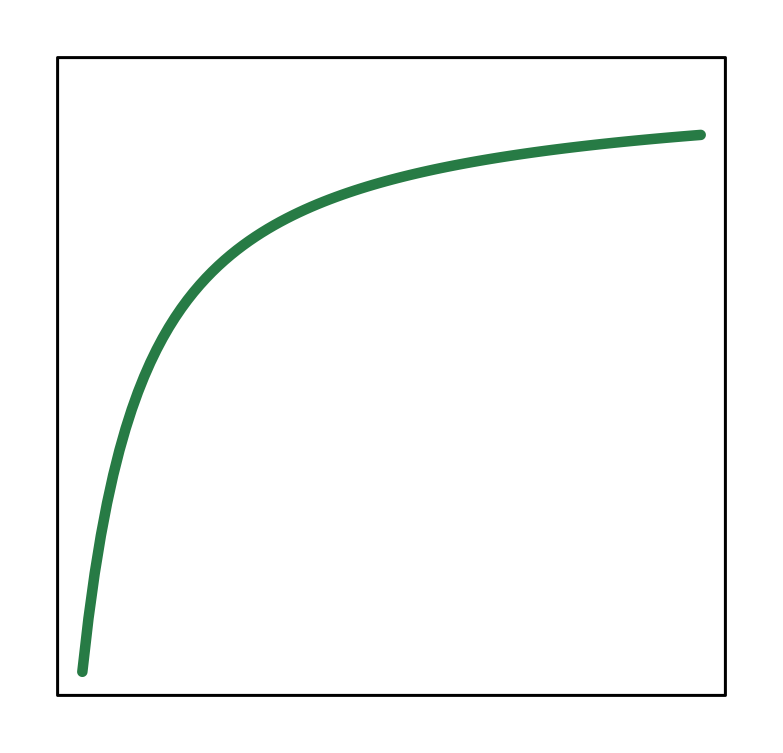
\includegraphics[width=2.60417in,height=\textheight]{Modellering/figuren/hill_small_t1.png} \\
Type III & \(\frac{x^2}{x^2+h^2}\) &
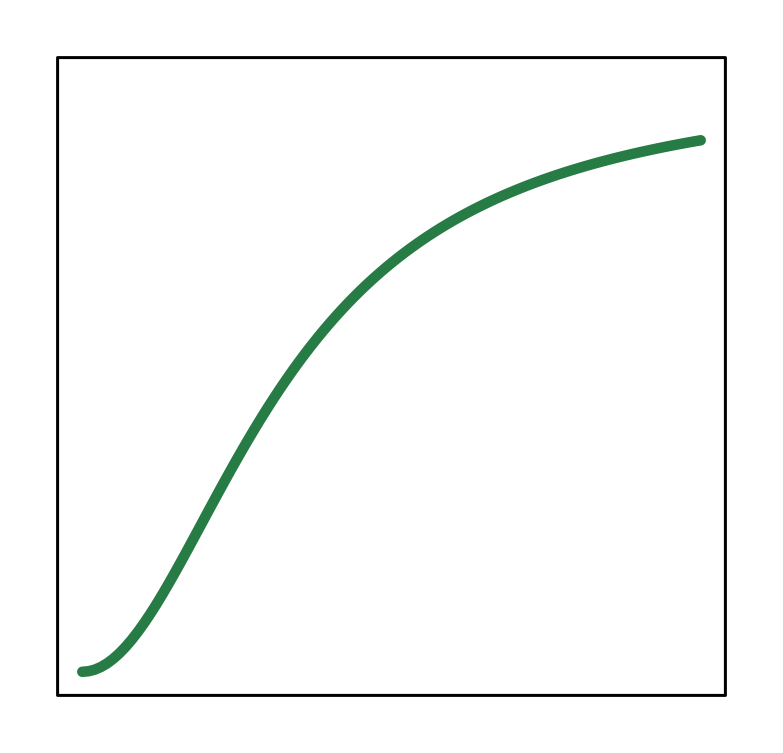
\includegraphics[width=2.60417in,height=\textheight]{Modellering/figuren/hill_small_t2.png} \\
Type II (afnemend) & \(\frac{1}{\frac{x}{h}+1}\) &
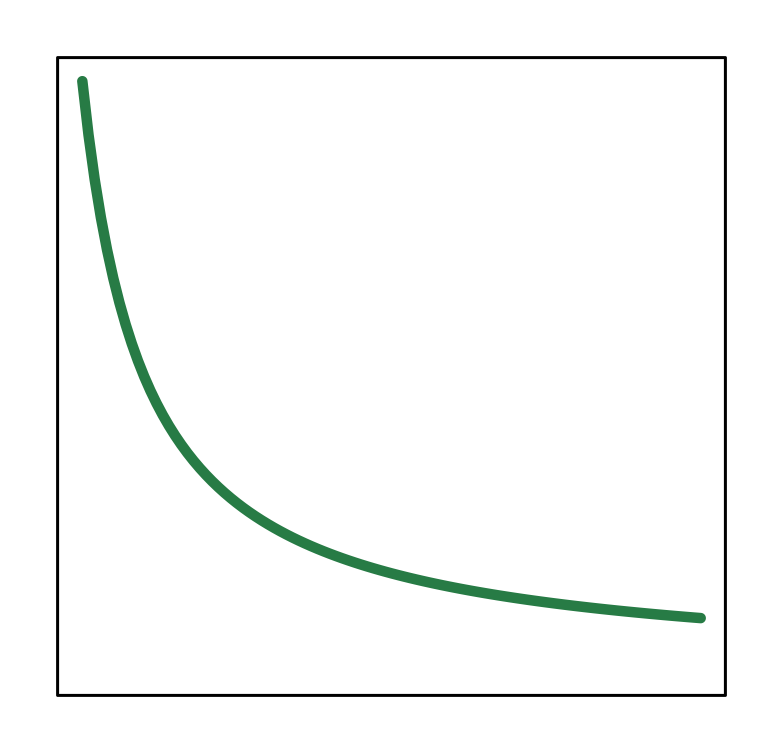
\includegraphics[width=2.60417in,height=\textheight]{Modellering/figuren/hill_small_inv_t1.png} \\
Type III (afnemend) & \(\frac{1}{\frac{x^2}{h^2}+1}\) &
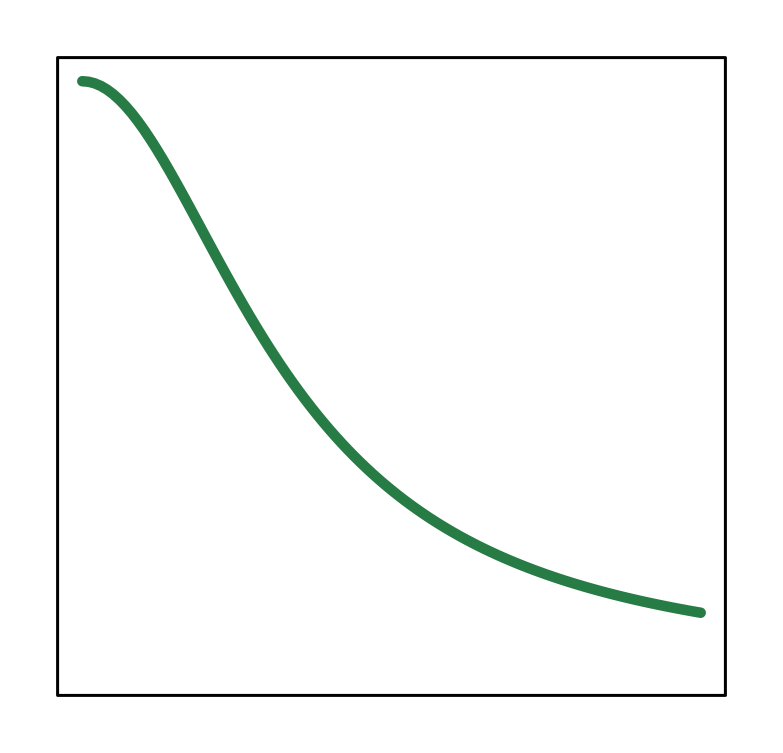
\includegraphics[width=2.60417in,height=\textheight]{Modellering/figuren/hill_small_inv_t2.png} \\
\end{longtable}

\end{tcolorbox}

\hypertarget{grind-tutorial}{%
\section{Grind tutorial}\label{grind-tutorial}}

Grind (\emph{GReat INtegrator Differential equations}) is een Rscript
geschreven door Rob de Boer (\url{https://tbb.bio.uu.nl/rdb}), wat het
heel makkelijk maakt om faseruimtes, vectorvelden, en oplossingen te
maken van ODE systemen. Ook kun je Grind gebruiken om modellen te fitten
aan experimentele data, zodat je op basis van metingen in het veld
parameters als \(b\), \(d\), \(K\), en \(h\) zou kunnen schatten. Dat
laatste is heel relevant wanneer modellen gebruikt worden voor
(bijvoorbeeld) belangrijke beleidsbeslissingen, maar in deze cursus gaan
we het vooral gebruiken om gemakkelijk faseruimtes met nullclines te
schetsen, en oplossingen te bestuderen. De volledige handleiding en
introductie tot Grind vind je
\href{https://tbb.bio.uu.nl/rdb/grindR/basics.html}{hier}.

Voordat je Grind kan gebruiken, moet je eenmalig een paar ``packages''
in R installeren:

\begin{Shaded}
\begin{Highlighting}[]
\CommentTok{\# Installeer de packages (hoeft maar 1 keer!)}
\FunctionTok{install.packages}\NormalTok{(}\StringTok{"FME"}\NormalTok{, }\StringTok{"deSolve"}\NormalTok{,}\StringTok{"coda"}\NormalTok{,}\StringTok{"rootSolve"}\NormalTok{) }
\end{Highlighting}
\end{Shaded}

Nadat deze packages zijn geinstalleerd, moeten we het Grind.R script
inladen. Dit kan je vanaf de website doen (zoals in het voorbeeld
hieronder), of je download het script zelf op je computer (dan hoef je
niet online te zijn!). Als alles goed is gegaan, krijg je een melding:

\begin{verbatim}
Warning: package 'deSolve' was built under R version 4.4.2
\end{verbatim}

\begin{verbatim}
Warning: package 'FME' was built under R version 4.4.2
\end{verbatim}

\begin{verbatim}
grind.R (25-06-2024) was sourced
\end{verbatim}

Nu kunnen we Grind.R gebruiken. De differentiaalvergelijkingen staan in
een functie genaamd `model'\footnote{Op regel 2 zie dat dat deze
  `model'-functie zit een beetje raar zit ingepakt in een \texttt{with}
  functie. Dit heeft een technische reden (en is zeker geen leerstof),
  maar helpt R begrijpen hoe de variabelen/parameters heten. De enige
  regels die je eigenlijk hoeft aan te passen zijn degene met de
  vergelijkingen (hier regel 3 en 4)}:

\begin{Shaded}
\begin{Highlighting}[numbers=left,,]
\NormalTok{model }\OtherTok{\textless{}{-}} \ControlFlowTok{function}\NormalTok{(t, state, parms) \{}
  \FunctionTok{with}\NormalTok{(}\FunctionTok{as.list}\NormalTok{(}\FunctionTok{c}\NormalTok{(state,parms)), \{}
\NormalTok{    dR }\OtherTok{\textless{}{-}}\NormalTok{ r}\SpecialCharTok{*}\NormalTok{R}\SpecialCharTok{*}\NormalTok{(}\DecValTok{1} \SpecialCharTok{{-}}\NormalTok{ R}\SpecialCharTok{/}\NormalTok{K) }\SpecialCharTok{{-}}\NormalTok{ a}\SpecialCharTok{*}\NormalTok{R}\SpecialCharTok{*}\NormalTok{N}\SpecialCharTok{/}\NormalTok{(R}\SpecialCharTok{+}\NormalTok{h)}
\NormalTok{    dN }\OtherTok{\textless{}{-}}\NormalTok{ c}\SpecialCharTok{*}\NormalTok{a}\SpecialCharTok{*}\NormalTok{R}\SpecialCharTok{*}\NormalTok{N}\SpecialCharTok{/}\NormalTok{(R}\SpecialCharTok{+}\NormalTok{h) }\SpecialCharTok{{-}}\NormalTok{ delta}\SpecialCharTok{*}\NormalTok{N}
    \FunctionTok{return}\NormalTok{(}\FunctionTok{list}\NormalTok{(}\FunctionTok{c}\NormalTok{(dR, dN)))  }
\NormalTok{  \}) }
\NormalTok{\}  }
\end{Highlighting}
\end{Shaded}

En vervolgens geef je de parameters en begin-waarden (\emph{initial
condition}) voor de variabelen aan:

\begin{Shaded}
\begin{Highlighting}[]
\NormalTok{p }\OtherTok{\textless{}{-}} \FunctionTok{c}\NormalTok{(}\AttributeTok{r=}\DecValTok{1}\NormalTok{,}\AttributeTok{K=}\DecValTok{1}\NormalTok{,}\AttributeTok{a=}\DecValTok{1}\NormalTok{,}\AttributeTok{c=}\DecValTok{1}\NormalTok{,}\AttributeTok{delta=}\FloatTok{0.3}\NormalTok{,}\AttributeTok{c=}\DecValTok{1}\NormalTok{,}\AttributeTok{h=}\DecValTok{1}\NormalTok{)  }\CommentTok{\#parameters}
\NormalTok{s }\OtherTok{\textless{}{-}} \FunctionTok{c}\NormalTok{(}\AttributeTok{R=}\DecValTok{1}\NormalTok{,}\AttributeTok{N=}\FloatTok{0.01}\NormalTok{) }\CommentTok{\#begin{-}dichtheden van R en N  }
\NormalTok{colors[}\DecValTok{1}\NormalTok{] }\OtherTok{=} \StringTok{"blue"}
\NormalTok{colors[}\DecValTok{2}\NormalTok{] }\OtherTok{=} \StringTok{"\#FF7F50"}
\end{Highlighting}
\end{Shaded}

Hierboven geef ik ook even de nieuwe kleuren aan voor de `eerste' en
`tweede' vergelijking, zodat dit overeenkomt met de kleuren die we tot
nu toe hebben gebruikt. Dit is niet noodzakelijk, maar zo raken we niet
in de war.

Nu kun je met met de functie \texttt{run} eenvoudig een oplossing
uitrekenen:

\begin{Shaded}
\begin{Highlighting}[]
\FunctionTok{run}\NormalTok{()}
\end{Highlighting}
\end{Shaded}

\begin{figure}[H]

{\centering 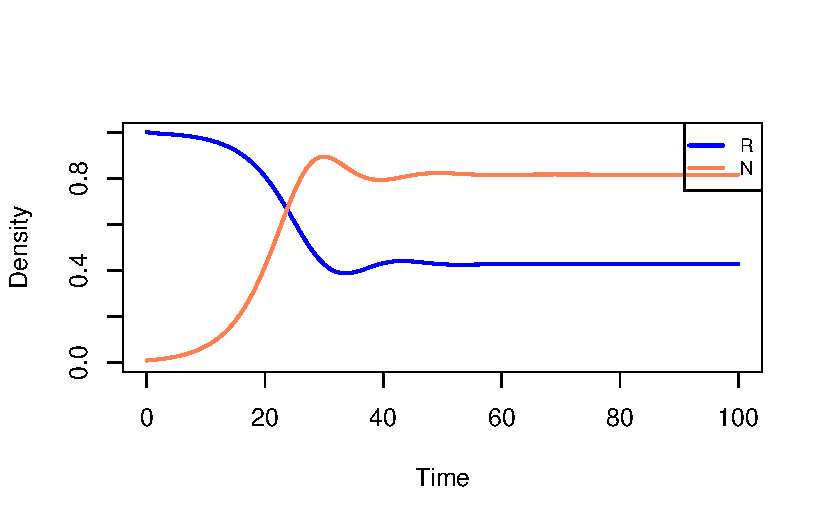
\includegraphics{Modellering/ecoevo_grindbif_files/figure-pdf/unnamed-chunk-8-1.pdf}

}

\end{figure}

\begin{verbatim}
        R         N 
0.4285768 0.8163156 
\end{verbatim}

Zoals je ziet genereert Grind een grafiek (een oplossing), en vertelt
het ook meteen wat de eind-waarden zijn van je variabelen.

We kunnen ook argumenten aan \texttt{run} meegeven, bijvoorbeeld om wat
langer door te rekenen (\texttt{tmax}, deze optie is standaard 100) en
een optie om y-as logaritmisch te schalen:

\begin{Shaded}
\begin{Highlighting}[]
\FunctionTok{run}\NormalTok{(}\AttributeTok{tmax=}\DecValTok{200}\NormalTok{,}\AttributeTok{log =} \StringTok{"y"}\NormalTok{) }
\end{Highlighting}
\end{Shaded}

\begin{figure}[H]

{\centering 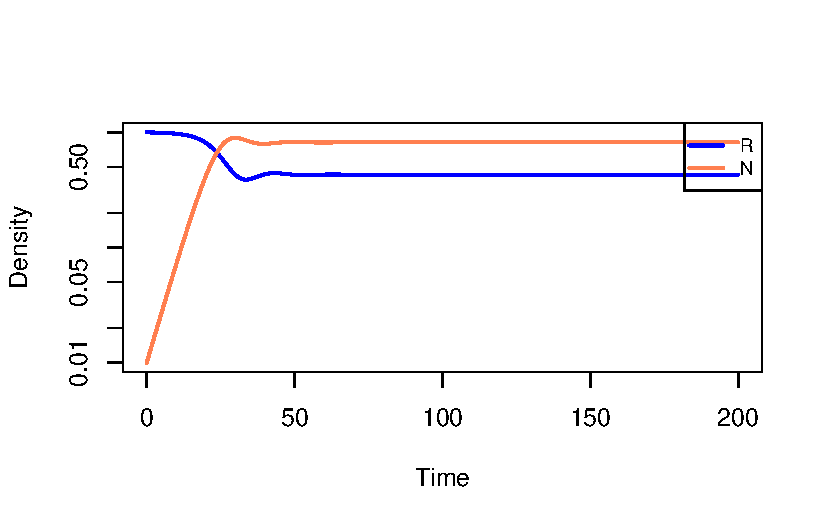
\includegraphics{Modellering/ecoevo_grindbif_files/figure-pdf/unnamed-chunk-9-1.pdf}

}

\end{figure}

\begin{verbatim}
        R         N 
0.4285714 0.8163265 
\end{verbatim}

Zoals je ziet zijn de waarden na tijdstip 100 niet meer veel veranderd.
Het systeem was dus eigenlijk al (bijna) in evenwicht.

We kunnen ook een faseruimte maken met de functie \texttt{plane}:

\begin{Shaded}
\begin{Highlighting}[]
\FunctionTok{plane}\NormalTok{() }
\end{Highlighting}
\end{Shaded}

\begin{figure}[H]

{\centering 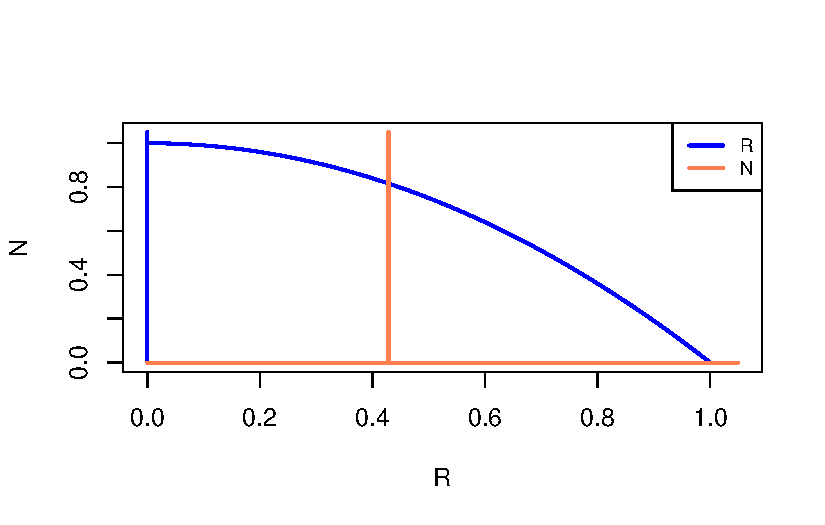
\includegraphics{Modellering/ecoevo_grindbif_files/figure-pdf/unnamed-chunk-10-1.pdf}

}

\end{figure}

Ook deze functie kunnen we weer argumenten meegeven, bijvoorbeeld om de
assen iets verder te vergroten, een vectorveld te tekenen:

\begin{Shaded}
\begin{Highlighting}[]
\FunctionTok{plane}\NormalTok{(}\AttributeTok{xmax=}\FloatTok{1.5}\NormalTok{, }\AttributeTok{ymax=}\FloatTok{1.5}\NormalTok{,}\AttributeTok{vector =}\NormalTok{ T) }
\end{Highlighting}
\end{Shaded}

\begin{figure}[H]

{\centering 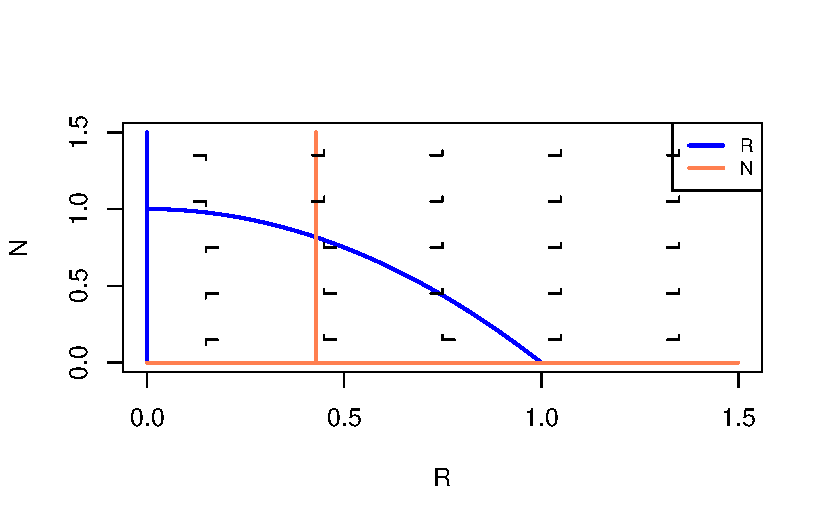
\includegraphics{Modellering/ecoevo_grindbif_files/figure-pdf/unnamed-chunk-11-1.pdf}

}

\end{figure}

Als laatste willen we (net als in het vorige hoofdstuk) weten of de
evenwichten stabiel of instabiel zijn. Hiervoor geven we Grind een
geschatte waarde dichtbij een evenwicht mee, en gebruiken we de functie
\texttt{newton}:

\begin{Shaded}
\begin{Highlighting}[]
\FunctionTok{plane}\NormalTok{(}\AttributeTok{xmax=}\FloatTok{1.5}\NormalTok{, }\AttributeTok{ymax=}\FloatTok{1.5}\NormalTok{,}\AttributeTok{vector =}\NormalTok{ T)}
\FunctionTok{newton}\NormalTok{(}\AttributeTok{state=}\FunctionTok{c}\NormalTok{(}\AttributeTok{R=}\FloatTok{0.0}\NormalTok{,}\AttributeTok{N=}\FloatTok{0.0}\NormalTok{),}\AttributeTok{plot=}\NormalTok{T)}
\FunctionTok{newton}\NormalTok{(}\AttributeTok{state=}\FunctionTok{c}\NormalTok{(}\AttributeTok{R=}\FloatTok{1.0}\NormalTok{,}\AttributeTok{N=}\FloatTok{0.0}\NormalTok{),}\AttributeTok{plot=}\NormalTok{T)}
\FunctionTok{newton}\NormalTok{(}\AttributeTok{state=}\FunctionTok{c}\NormalTok{(}\AttributeTok{R=}\FloatTok{0.4}\NormalTok{,}\AttributeTok{N=}\FloatTok{0.8}\NormalTok{),}\AttributeTok{plot=}\NormalTok{T)}
\FunctionTok{run}\NormalTok{(}\AttributeTok{traject =}\NormalTok{ T)}
\end{Highlighting}
\end{Shaded}

\begin{figure}[H]

{\centering 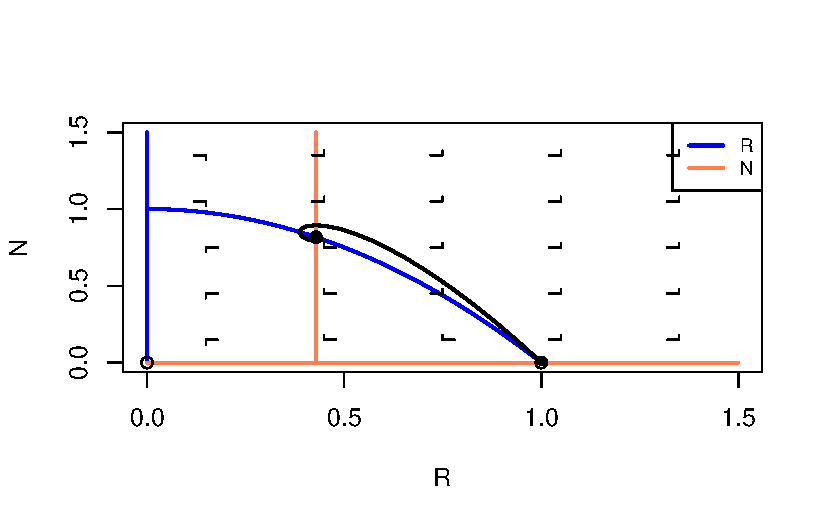
\includegraphics{Modellering/ecoevo_grindbif_files/figure-pdf/unnamed-chunk-12-1.pdf}

}

\end{figure}

De laatste regel gebruikt \texttt{run} met de optie \texttt{traject=T}
om een trajectorie door de faseruimte te tekenen. Dit vertaalt het
grafiekje door de tijd die we eerder hebben uitgerekend, naar een mooie
inwaardse spiraal. Er zijn nog
\href{https://tbb.bio.uu.nl/rdb/grindR/basics.html}{veel meer opties} in
Grind.R. Als je wil zien welke argumenten een functie allemaal kent, kun
je gebruik maken van \texttt{args}:

\begin{Shaded}
\begin{Highlighting}[]
\FunctionTok{args}\NormalTok{(plane)}
\end{Highlighting}
\end{Shaded}

\begin{verbatim}
function (xmin = -0.001, xmax = 1.05, ymin = -0.001, ymax = 1.05, 
    xlab = "", ylab = "", log = "", npixels = 500, state = s, 
    parms = p, odes = model, x = 1, y = 2, time = 0, grid = 5, 
    eps = NULL, show = NULL, addone = FALSE, portrait = FALSE, 
    vector = FALSE, add = FALSE, legend = TRUE, zero = TRUE, 
    lwd = 2, col = "black", pch = 20, ...) 
NULL
\end{verbatim}

Zo zie je bijvoorbeeld dat je de legenda zou kunnen verbergen met de
\texttt{legend} optie, of de lijndikte (\texttt{lwd}) zou kunnen
aanpassen. Met andere woorden: met R kunnen we zonder al te veel
rekenwerk prachtige figuren genereren en wiskundige modellen
doorrekenen!

\hypertarget{lotka-volterra-in-grind}{%
\section{Lotka-Volterra in Grind}\label{lotka-volterra-in-grind}}

Als je de bovenstaande tutorial hebt gevolgd (en de packages hebt
geïnstalleerd), kun je nu het volgende script overnemen en aan de slag
met het Lotka-Volterra model:

\begin{Shaded}
\begin{Highlighting}[numbers=left,,]
\NormalTok{model }\OtherTok{\textless{}{-}} \ControlFlowTok{function}\NormalTok{(t, state, parms) \{}
  \FunctionTok{with}\NormalTok{(}\FunctionTok{as.list}\NormalTok{(}\FunctionTok{c}\NormalTok{(state,parms)), \{}
\NormalTok{    dR }\OtherTok{\textless{}{-}}\NormalTok{ r}\SpecialCharTok{*}\NormalTok{R}\SpecialCharTok{*}\NormalTok{(}\DecValTok{1} \SpecialCharTok{{-}}\NormalTok{ R}\SpecialCharTok{/}\NormalTok{K) }\SpecialCharTok{{-}}\NormalTok{ a}\SpecialCharTok{*}\NormalTok{R}\SpecialCharTok{*}\NormalTok{N}\SpecialCharTok{/}\NormalTok{(R}\SpecialCharTok{+}\NormalTok{h)}
\NormalTok{    dN }\OtherTok{\textless{}{-}}\NormalTok{ c}\SpecialCharTok{*}\NormalTok{a}\SpecialCharTok{*}\NormalTok{R}\SpecialCharTok{*}\NormalTok{N}\SpecialCharTok{/}\NormalTok{(R}\SpecialCharTok{+}\NormalTok{h) }\SpecialCharTok{{-}}\NormalTok{ delta}\SpecialCharTok{*}\NormalTok{N}
    \FunctionTok{return}\NormalTok{(}\FunctionTok{list}\NormalTok{(}\FunctionTok{c}\NormalTok{(dR, dN)))  }
\NormalTok{  \}) }
\NormalTok{\}  }
\NormalTok{p }\OtherTok{\textless{}{-}} \FunctionTok{c}\NormalTok{(}\AttributeTok{r=}\DecValTok{1}\NormalTok{,}\AttributeTok{K=}\DecValTok{2}\NormalTok{,}\AttributeTok{a=}\DecValTok{1}\NormalTok{,}\AttributeTok{c=}\DecValTok{1}\NormalTok{,}\AttributeTok{delta=}\FloatTok{0.3}\NormalTok{,}\AttributeTok{c=}\DecValTok{1}\NormalTok{,}\AttributeTok{h=}\DecValTok{1}\NormalTok{)  }\CommentTok{\#parameters}
\NormalTok{s }\OtherTok{\textless{}{-}} \FunctionTok{c}\NormalTok{(}\AttributeTok{R=}\DecValTok{1}\NormalTok{,}\AttributeTok{N=}\FloatTok{0.01}\NormalTok{) }\CommentTok{\#begin{-}dichtheden van R en N  }

\NormalTok{colors[}\DecValTok{1}\NormalTok{] }\OtherTok{=} \StringTok{"blue"} \CommentTok{\#optioneel, default = \textquotesingle{}red\textquotesingle{}}
\NormalTok{colors[}\DecValTok{2}\NormalTok{] }\OtherTok{=} \StringTok{"\#FF7F50"} \CommentTok{\#optioneel, default = \textquotesingle{}blue\textquotesingle{}}
\FunctionTok{par}\NormalTok{(}\AttributeTok{mfrow=}\FunctionTok{c}\NormalTok{(}\DecValTok{1}\NormalTok{,}\DecValTok{2}\NormalTok{)) }\CommentTok{\# optioneel, maakt 2 plotjes naast elkaar}

\FunctionTok{plane}\NormalTok{(}\AttributeTok{xmax=}\DecValTok{3}\NormalTok{,}\AttributeTok{ymax=}\DecValTok{2}\NormalTok{)}
\FunctionTok{run}\NormalTok{(}\AttributeTok{tstep=}\FloatTok{0.5}\NormalTok{, }\AttributeTok{legend=}\NormalTok{F)}
\end{Highlighting}
\end{Shaded}

\begin{figure}[H]

{\centering 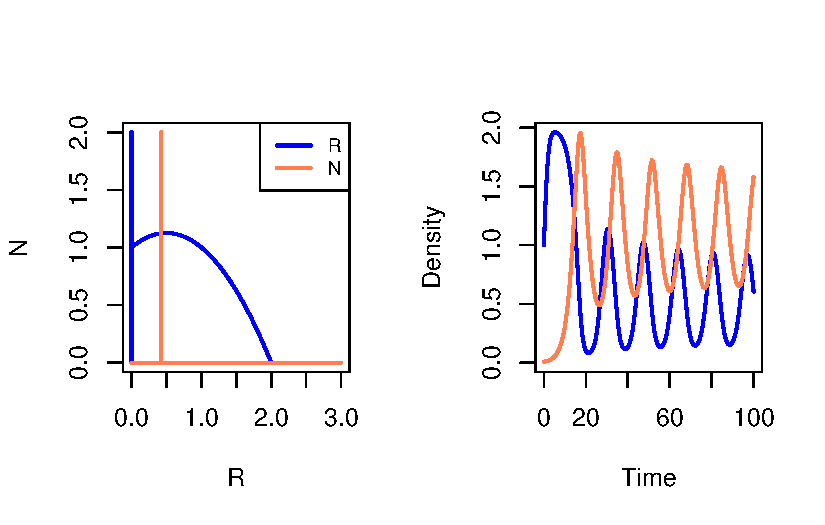
\includegraphics{Modellering/ecoevo_grindbif_files/figure-pdf/unnamed-chunk-14-1.pdf}

}

\end{figure}

\begin{verbatim}
       R        N 
0.605847 1.582674 
\end{verbatim}

Door te oefenen met dit R-script, naast de pen-en-papier opgaven, is het
de bedoeling dat je een goed gevoel ontwikkeld voor ODEs: simpele,
wiskundige modellen, die veel in de biologische literatuur voorkomen.
Hieronder volgt een korte vraag, om met zowel pen-en-papier als Grind te
oefenen.

\begin{exercise}[De nieuwe nullcline voor de
prooi]\protect\hypertarget{exr-paraboollv}{}\label{exr-paraboollv}

Hierboven hebben we nullclines gegenereerd van het vernieuwde
Lotka-Volterra model (met een verzadigbare predator). Zoals je ziet is
dit geen rechte lijn meer.

\begin{enumerate}
\def\labelenumi{\alph{enumi}.}
\tightlist
\item
  Bepaal met pen-en-papier aan welke functie de vernieuwde nullcline
  voor de prooi voldoet.
\item
  Wat is het effect van de \(K\) parameter op de ligging van deze
  nullcline?
\item
  Neem het R-script hierboven over met het Lotka-Volterra model met
  verzadigbare predator. Verdubbel de waarde van \(K\). Wat valt je op?
\end{enumerate}

\end{exercise}

\hypertarget{bifurcaties-van-evenwichten}{%
\section{Bifurcaties van
evenwichten}\label{bifurcaties-van-evenwichten}}

Het bovenstaande Lotka-Volterra model heeft een interessant eigenschap:
afhankelijk van de parameters kan het type evenwicht veranderen. Iets
dergelijks zagen we ook al eerder terug: de predator kon alleen
samenleven met de prooi als de parameters dat toelieten. Deze transitie
zien we ook terug in dit vernieuwde model (van
Figuur~\ref{fig-lvvoort-1} naar Figuur~\ref{fig-lvvoort-2}). Deze
bifurcatie (van geen samenleving naar wél samenleving) wordt een
\textbf{critische transitie} genoemd. Echter is er met dit vernieuwde
model een tweede bifurcatie mogelijk: de predator-nullcline kan de
prooi-nulllcine links of rechts van de top van de parabool snijden (van
Figuur~\ref{fig-lvvoort-2} naar Figuur~\ref{fig-lvvoort-3}). Als het
snijpunt links van de parabool ligt, zien we voortdurende oscillaties
van predator en prooi. Deze specifieke bifurcatie staat bekend als de
\textbf{Hopf-bifurcatie}.

\begin{Shaded}
\begin{Highlighting}[]
\NormalTok{model }\OtherTok{\textless{}{-}} \ControlFlowTok{function}\NormalTok{(t, state, parms) \{}
  \FunctionTok{with}\NormalTok{(}\FunctionTok{as.list}\NormalTok{(}\FunctionTok{c}\NormalTok{(state,parms)), \{}
\NormalTok{    dR }\OtherTok{\textless{}{-}}\NormalTok{ r}\SpecialCharTok{*}\NormalTok{R}\SpecialCharTok{*}\NormalTok{(}\DecValTok{1} \SpecialCharTok{{-}}\NormalTok{ R}\SpecialCharTok{/}\NormalTok{K) }\SpecialCharTok{{-}}\NormalTok{ a}\SpecialCharTok{*}\NormalTok{R}\SpecialCharTok{*}\NormalTok{N}\SpecialCharTok{/}\NormalTok{(R}\SpecialCharTok{+}\NormalTok{h)}
\NormalTok{    dN }\OtherTok{\textless{}{-}}\NormalTok{ c}\SpecialCharTok{*}\NormalTok{a}\SpecialCharTok{*}\NormalTok{R}\SpecialCharTok{*}\NormalTok{N}\SpecialCharTok{/}\NormalTok{(R}\SpecialCharTok{+}\NormalTok{h) }\SpecialCharTok{{-}}\NormalTok{ delta}\SpecialCharTok{*}\NormalTok{N}
    \FunctionTok{return}\NormalTok{(}\FunctionTok{list}\NormalTok{(}\FunctionTok{c}\NormalTok{(dR, dN)))  }
\NormalTok{  \}) }
\NormalTok{\}  }

\NormalTok{colors[}\DecValTok{1}\NormalTok{] }\OtherTok{=} \StringTok{"blue"} \CommentTok{\#optioneel, default = \textquotesingle{}red\textquotesingle{}}
\NormalTok{colors[}\DecValTok{2}\NormalTok{] }\OtherTok{=} \StringTok{"\#FF7F50"} \CommentTok{\#optioneel, default = \textquotesingle{}blue\textquotesingle{}}

\NormalTok{p }\OtherTok{\textless{}{-}} \FunctionTok{c}\NormalTok{(}\AttributeTok{r=}\DecValTok{1}\NormalTok{,}\AttributeTok{K=}\FloatTok{0.4}\NormalTok{,}\AttributeTok{a=}\DecValTok{1}\NormalTok{,}\AttributeTok{c=}\DecValTok{1}\NormalTok{,}\AttributeTok{delta=}\FloatTok{0.3}\NormalTok{,}\AttributeTok{c=}\DecValTok{1}\NormalTok{,}\AttributeTok{h=}\DecValTok{1}\NormalTok{)  }\CommentTok{\#parameters}
\NormalTok{s }\OtherTok{\textless{}{-}} \FunctionTok{c}\NormalTok{(}\AttributeTok{R=}\FloatTok{0.4}\NormalTok{,}\AttributeTok{N=}\FloatTok{0.01}\NormalTok{) }\CommentTok{\#begin{-}dichtheden van R en N  }
\FunctionTok{plane}\NormalTok{(}\AttributeTok{xmax=}\FloatTok{2.2}\NormalTok{,}\AttributeTok{ymax=}\DecValTok{2}\NormalTok{)}
\FunctionTok{run}\NormalTok{(}\AttributeTok{tstep=}\FloatTok{0.5}\NormalTok{, }\AttributeTok{traject=}\NormalTok{T,}\AttributeTok{col=}\StringTok{"grey"}\NormalTok{)}
\FunctionTok{newton}\NormalTok{(}\AttributeTok{state=}\FunctionTok{c}\NormalTok{(}\AttributeTok{R=}\FloatTok{0.5}\NormalTok{,}\AttributeTok{N=}\FloatTok{0.5}\NormalTok{),}\AttributeTok{plot=}\NormalTok{T)}

\NormalTok{p }\OtherTok{\textless{}{-}} \FunctionTok{c}\NormalTok{(}\AttributeTok{r=}\DecValTok{1}\NormalTok{,}\AttributeTok{K=}\DecValTok{1}\NormalTok{,}\AttributeTok{a=}\DecValTok{1}\NormalTok{,}\AttributeTok{c=}\DecValTok{1}\NormalTok{,}\AttributeTok{delta=}\FloatTok{0.3}\NormalTok{,}\AttributeTok{c=}\DecValTok{1}\NormalTok{,}\AttributeTok{h=}\DecValTok{1}\NormalTok{)  }\CommentTok{\#parameters}
\NormalTok{s }\OtherTok{\textless{}{-}} \FunctionTok{c}\NormalTok{(}\AttributeTok{R=}\DecValTok{2}\NormalTok{,}\AttributeTok{N=}\FloatTok{0.01}\NormalTok{) }\CommentTok{\#begin{-}dichtheden van R en N  }
\FunctionTok{plane}\NormalTok{(}\AttributeTok{xmax=}\FloatTok{2.2}\NormalTok{,}\AttributeTok{ymax=}\DecValTok{2}\NormalTok{)}
\FunctionTok{run}\NormalTok{(}\AttributeTok{tstep=}\FloatTok{0.5}\NormalTok{, }\AttributeTok{traject=}\NormalTok{T,}\AttributeTok{col=}\StringTok{"grey"}\NormalTok{)}
\FunctionTok{newton}\NormalTok{(}\AttributeTok{state=}\FunctionTok{c}\NormalTok{(}\AttributeTok{R=}\FloatTok{0.5}\NormalTok{,}\AttributeTok{N=}\FloatTok{0.5}\NormalTok{),}\AttributeTok{plot=}\NormalTok{T)}

\NormalTok{p }\OtherTok{\textless{}{-}} \FunctionTok{c}\NormalTok{(}\AttributeTok{r=}\DecValTok{1}\NormalTok{,}\AttributeTok{K=}\DecValTok{2}\NormalTok{,}\AttributeTok{a=}\DecValTok{1}\NormalTok{,}\AttributeTok{c=}\DecValTok{1}\NormalTok{,}\AttributeTok{delta=}\FloatTok{0.3}\NormalTok{,}\AttributeTok{c=}\DecValTok{1}\NormalTok{,}\AttributeTok{h=}\DecValTok{1}\NormalTok{)  }\CommentTok{\#parameters}
\NormalTok{s }\OtherTok{\textless{}{-}} \FunctionTok{c}\NormalTok{(}\AttributeTok{R=}\DecValTok{2}\NormalTok{,}\AttributeTok{N=}\FloatTok{0.01}\NormalTok{) }\CommentTok{\#begin{-}dichtheden van R en N  }
\FunctionTok{plane}\NormalTok{(}\AttributeTok{xmax=}\FloatTok{2.2}\NormalTok{,}\AttributeTok{ymax=}\DecValTok{2}\NormalTok{)}
\FunctionTok{run}\NormalTok{(}\AttributeTok{tstep=}\FloatTok{0.5}\NormalTok{, }\AttributeTok{traject=}\NormalTok{T,}\AttributeTok{col=}\StringTok{"grey"}\NormalTok{)}
\FunctionTok{newton}\NormalTok{(}\AttributeTok{state=}\FunctionTok{c}\NormalTok{(}\AttributeTok{R=}\FloatTok{0.5}\NormalTok{,}\AttributeTok{N=}\FloatTok{0.5}\NormalTok{),}\AttributeTok{plot=}\NormalTok{T)}
\end{Highlighting}
\end{Shaded}

\begin{figure}

\begin{minipage}[t]{0.33\linewidth}

{\centering 

\raisebox{-\height}{

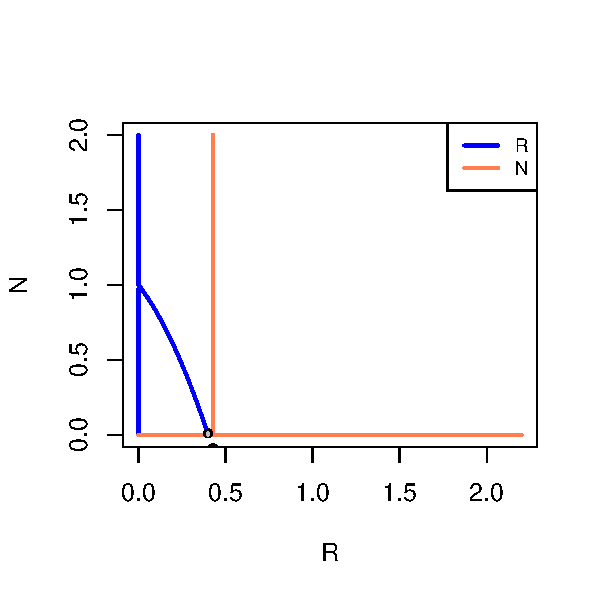
\includegraphics{Modellering/ecoevo_grindbif_files/figure-pdf/fig-lvvoort-1.pdf}

}

}

\subcaption{\label{fig-lvvoort-1}Als de nullclines niet snijden, is er
geen evenwicht.}
\end{minipage}%
%
\begin{minipage}[t]{0.33\linewidth}

{\centering 

\raisebox{-\height}{

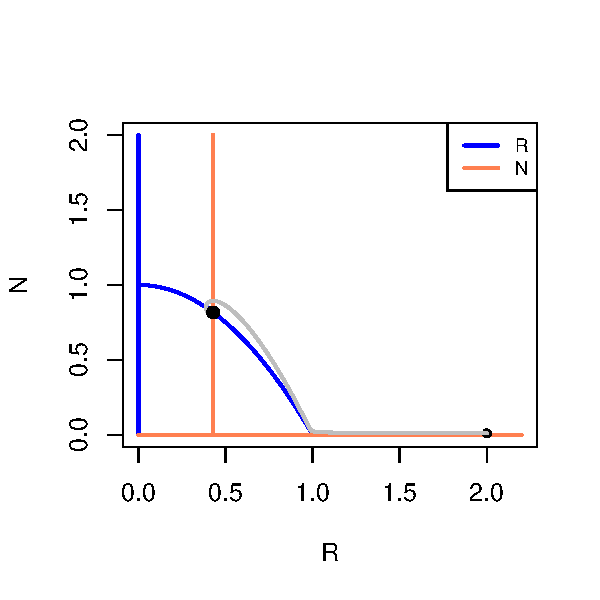
\includegraphics{Modellering/ecoevo_grindbif_files/figure-pdf/fig-lvvoort-2.pdf}

}

}

\subcaption{\label{fig-lvvoort-2}Vertrouwde inwaarde spiraal die naar
een stabiel evenwicht gaat.}
\end{minipage}%
%
\begin{minipage}[t]{0.33\linewidth}

{\centering 

\raisebox{-\height}{

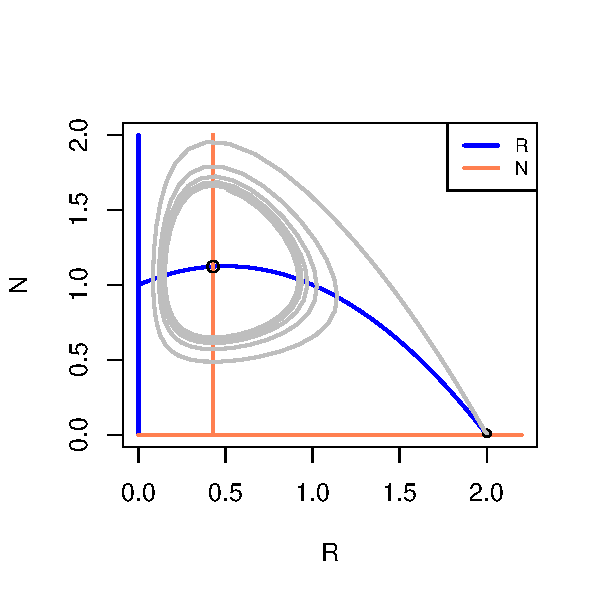
\includegraphics{Modellering/ecoevo_grindbif_files/figure-pdf/fig-lvvoort-3.pdf}

}

}

\subcaption{\label{fig-lvvoort-3}Voortdurende oscillaties rond een
instabiel evenwicht.}
\end{minipage}%

\caption{\label{fig-lvvoort}\textbf{?(caption)}}

\end{figure}

Voortdurende oscillaties tussen prooi en predator worden inderdaad
waargenomen, bijvoorbeeld de oscillaties tussen hazen en lynxen in Noord
Amerika (Figuur~\ref{fig-hazenenlynxen}). Ook experimenteel zijn
dergelijke oscillaties waargenomen, bijvoorbeeld door \emph{Paramecium}
(een-cellige protist, prooi) en \emph{Didinium} (eencellige protist,
predator) samen te groeien in een Erlenmeyer (Xia \emph{et al.}, 1992,
\textbf{INSERT REFERENCE}).

\begin{figure}

{\centering 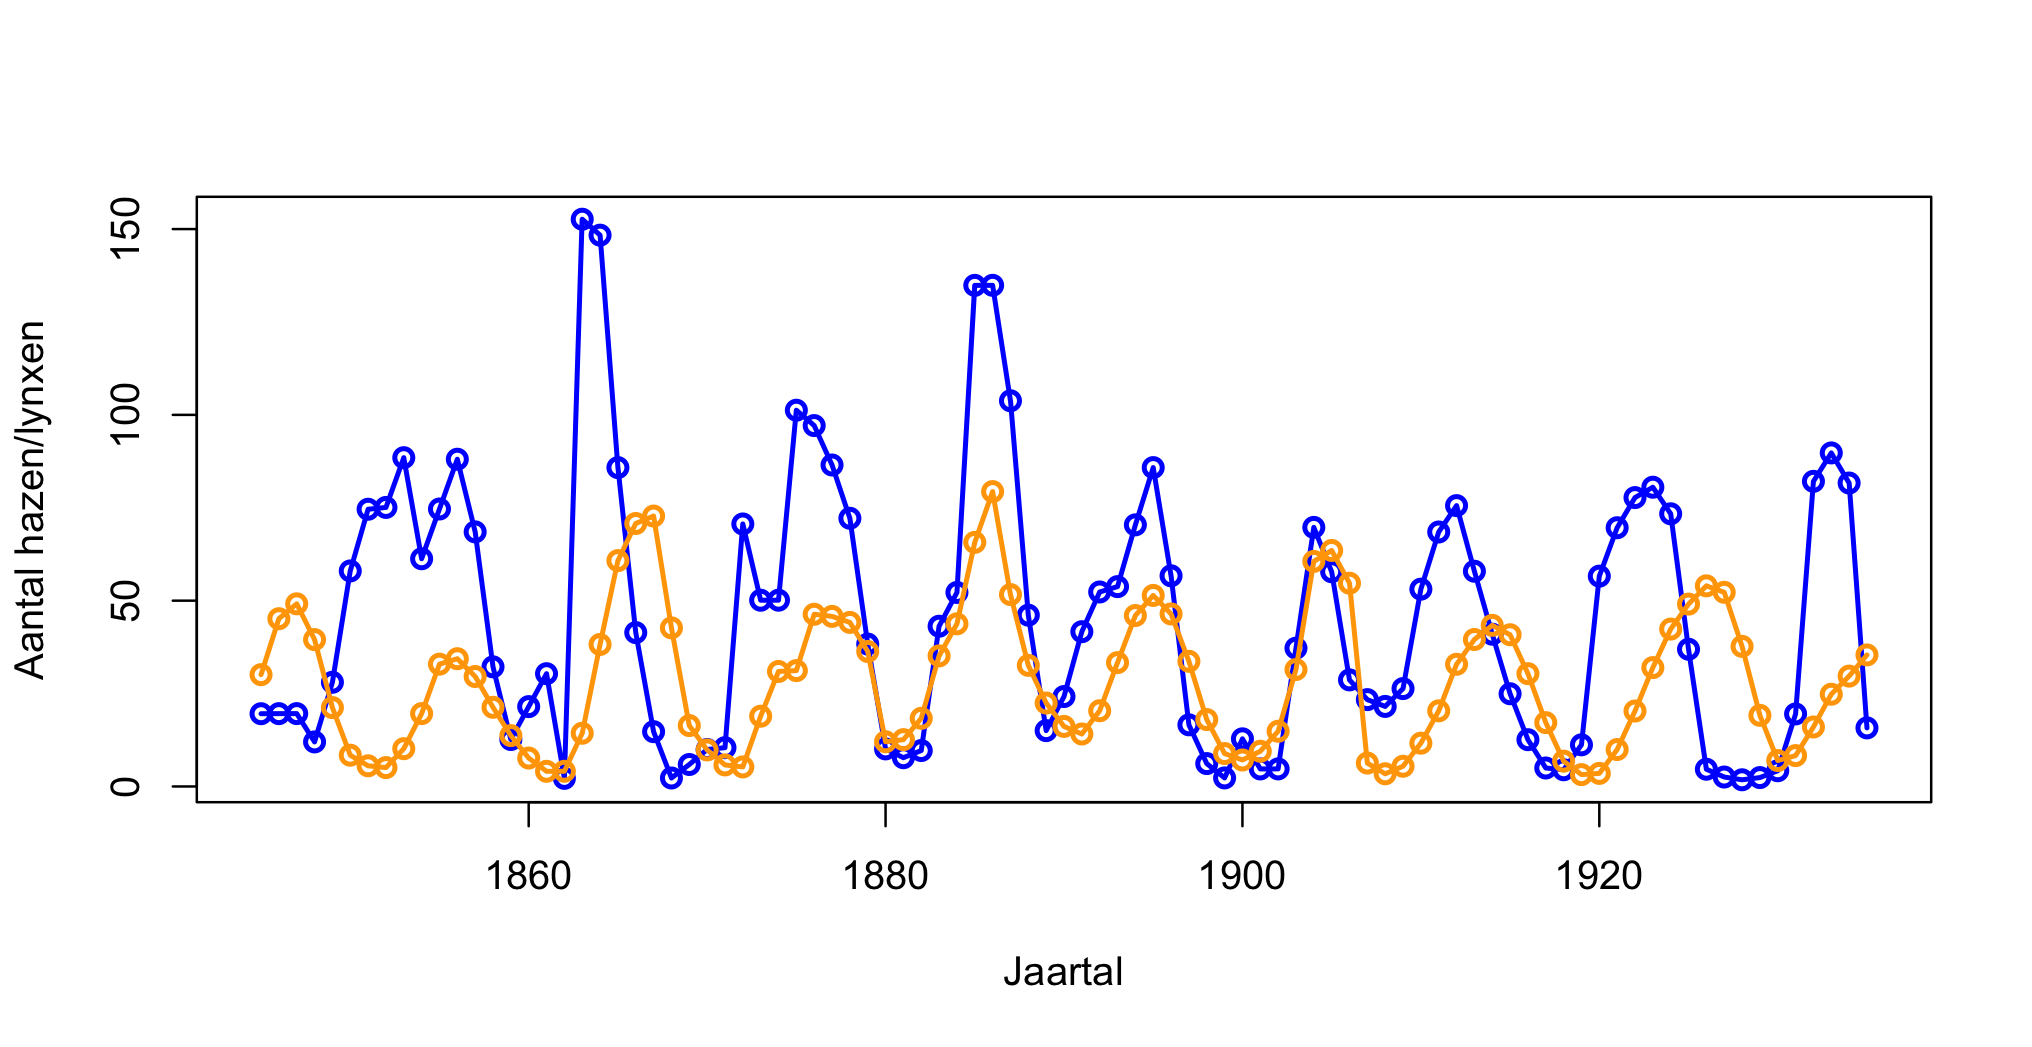
\includegraphics{Modellering/figuren/hazen_en_lynxen.png}

}

\caption{\label{fig-hazenenlynxen}Populatieaantallen hazen en lynxen in
Noord Amerika van medio 19e eeuw tot medio 20e eeuw (bepaald op basis
van de vachten-verkoop)}

\end{figure}

Bifurcaties kun je weergeven in een bifurcatiediagram, waarbij we de
parameter die het evenwicht beinvloed op de x-as zetten, en de
populatiegroottes in evenwicht op de y-as. Als we dit doen voor de
bovenstaande bifurcaties, krijgen we dit:

\begin{Shaded}
\begin{Highlighting}[]
\FunctionTok{source}\NormalTok{(}\StringTok{"https://tbb.bio.uu.nl/rdb/grindR/grind.R"}\NormalTok{)}
\FunctionTok{library}\NormalTok{(ggplot2)}
\FunctionTok{library}\NormalTok{(dplyr)}
\end{Highlighting}
\end{Shaded}

\begin{verbatim}

Attaching package: 'dplyr'
\end{verbatim}

\begin{verbatim}
The following objects are masked from 'package:stats':

    filter, lag
\end{verbatim}

\begin{verbatim}
The following objects are masked from 'package:base':

    intersect, setdiff, setequal, union
\end{verbatim}

\begin{Shaded}
\begin{Highlighting}[]
\NormalTok{my\_theme }\OtherTok{\textless{}{-}} \FunctionTok{theme\_bw}\NormalTok{() }\SpecialCharTok{+} 
  \FunctionTok{theme}\NormalTok{(}\AttributeTok{panel.border =} \FunctionTok{element\_blank}\NormalTok{(), }\AttributeTok{panel.grid.major =} \FunctionTok{element\_blank}\NormalTok{(),}
        \AttributeTok{panel.grid.minor =} \FunctionTok{element\_blank}\NormalTok{(), }\AttributeTok{axis.line =} \FunctionTok{element\_line}\NormalTok{(}\AttributeTok{colour =} \StringTok{"black"}\NormalTok{))}

  
\NormalTok{model }\OtherTok{\textless{}{-}} \ControlFlowTok{function}\NormalTok{(t, state, parms)\{}
  \FunctionTok{with}\NormalTok{(}\FunctionTok{as.list}\NormalTok{(}\FunctionTok{c}\NormalTok{(state,parms)),\{}
\NormalTok{    dR }\OtherTok{\textless{}{-}}\NormalTok{ R}\SpecialCharTok{*}\NormalTok{(b}\SpecialCharTok{*}\NormalTok{(}\DecValTok{1}\SpecialCharTok{{-}}\NormalTok{R}\SpecialCharTok{/}\NormalTok{K)}\SpecialCharTok{{-}}\NormalTok{d) }\SpecialCharTok{{-}}\NormalTok{ a}\SpecialCharTok{*}\NormalTok{R}\SpecialCharTok{*}\NormalTok{N}\SpecialCharTok{/}\NormalTok{(R}\SpecialCharTok{+}\NormalTok{h)}
\NormalTok{    dN }\OtherTok{\textless{}{-}}\NormalTok{ c}\SpecialCharTok{*}\NormalTok{a}\SpecialCharTok{*}\NormalTok{R}\SpecialCharTok{*}\NormalTok{N}\SpecialCharTok{/}\NormalTok{(R}\SpecialCharTok{+}\NormalTok{h) }\SpecialCharTok{{-}}\NormalTok{ delta}\SpecialCharTok{*}\NormalTok{N}
    \FunctionTok{return}\NormalTok{(}\FunctionTok{list}\NormalTok{(}\FunctionTok{c}\NormalTok{(dR,dN)))}
\NormalTok{  \})}
\NormalTok{\}  }


\CommentTok{\# all \textless{}{-} data.frame()}
\CommentTok{\# for(k in c(0.00001,seq(0.001,4.0,by=0.001)))\{}
\CommentTok{\#   p \textless{}{-} c(a=0.5,delta=0.25,b=0.5,d=0.01,c=0.99,K=k,h=1)}
\CommentTok{\#   s \textless{}{-} c(R=0.4,N=0.4)}
\CommentTok{\#   plane(ymax=1.2,ymin={-}0.1,xmin={-}0.01, xmax=1.2,tstep=0.01,tmax=50)}
\CommentTok{\#   \#res \textless{}{-} newton()}
\CommentTok{\#   dat \textless{}{-} run(table=T,step=11,tmax=1000,timeplot=F)}
\CommentTok{\#   dat$K = k}
\CommentTok{\#   all \textless{}{-} rbind(all,tail(dat,100))}
\CommentTok{\#   cat(k,"\textbackslash{}n")}
\CommentTok{\# \}}
\CommentTok{\# }
\CommentTok{\# bifurcation\_data \textless{}{-} all \%\textgreater{}\% group\_by(K) \%\textgreater{}\% }
\CommentTok{\#   mutate(maxN=max(N)) \%\textgreater{}\% }
\CommentTok{\#   mutate(minN=min(N)) \%\textgreater{}\% }
\CommentTok{\#   mutate(maxR=max(R)) \%\textgreater{}\% }
\CommentTok{\#   mutate(minR=min(R)) \%\textgreater{}\% }
\CommentTok{\#   filter(time==1000) \%\textgreater{}\% }
\CommentTok{\#   distinct()}
\CommentTok{\# }
\CommentTok{\# write.table(bifurcation\_data, "Modellering/figuren/bifurcation\_data.csv")}

\NormalTok{bifurcation\_data }\OtherTok{\textless{}{-}} \FunctionTok{read.table}\NormalTok{(}\StringTok{"figuren/bifurcation\_data.csv"}\NormalTok{)}
\CommentTok{\#list.files("figuren")}

\NormalTok{colors }\OtherTok{\textless{}{-}} \FunctionTok{c}\NormalTok{(}\StringTok{"R"} \OtherTok{=} \StringTok{"blue"}\NormalTok{, }\StringTok{"N"} \OtherTok{=} \StringTok{"\#FF7F50"}\NormalTok{)}

\NormalTok{bifurcation\_data }\SpecialCharTok{\%\textgreater{}\%}
  \FunctionTok{ggplot}\NormalTok{(}\FunctionTok{aes}\NormalTok{(}\AttributeTok{x=}\NormalTok{K,}\AttributeTok{y=}\NormalTok{maxN)) }\SpecialCharTok{+}
  \CommentTok{\#geom\_line(col="\#FF7F50",linewidth=1, aes(color="N")) +}
  \FunctionTok{geom\_line}\NormalTok{(}\FunctionTok{aes}\NormalTok{(}\AttributeTok{y=}\NormalTok{maxR,}\AttributeTok{color=}\StringTok{"R"}\NormalTok{),}\AttributeTok{linewidth=}\DecValTok{1}\NormalTok{) }\SpecialCharTok{+}
  \FunctionTok{geom\_line}\NormalTok{(}\FunctionTok{aes}\NormalTok{(}\AttributeTok{y=}\NormalTok{minR,}\AttributeTok{color=}\StringTok{"R"}\NormalTok{),}\AttributeTok{linewidth=}\DecValTok{1}\NormalTok{) }\SpecialCharTok{+}
  \FunctionTok{geom\_line}\NormalTok{(}\FunctionTok{aes}\NormalTok{(}\AttributeTok{y=}\NormalTok{minN,}\AttributeTok{color=}\StringTok{"N"}\NormalTok{),}\AttributeTok{linewidth=}\DecValTok{1}\NormalTok{) }\SpecialCharTok{+}
  \FunctionTok{geom\_line}\NormalTok{(}\FunctionTok{aes}\NormalTok{(}\AttributeTok{y=}\NormalTok{maxN,}\AttributeTok{color=}\StringTok{"N"}\NormalTok{),}\AttributeTok{linewidth=}\DecValTok{1}\NormalTok{) }\SpecialCharTok{+}
  \FunctionTok{ylab}\NormalTok{(}\StringTok{"Steady state population sizes"}\NormalTok{) }\SpecialCharTok{+}
\NormalTok{  my\_theme }\SpecialCharTok{+}
  \FunctionTok{scale\_color\_manual}\NormalTok{(}\AttributeTok{name=}\StringTok{"Soort"}\NormalTok{,}\AttributeTok{values =}\NormalTok{ colors)}
\end{Highlighting}
\end{Shaded}

\begin{figure}[H]

{\centering 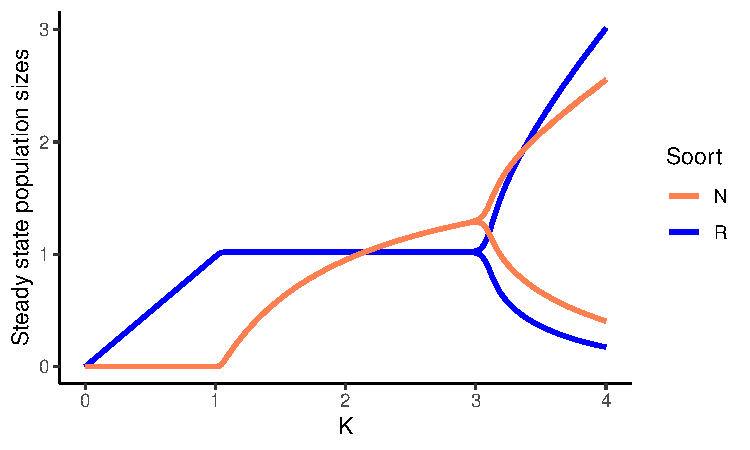
\includegraphics{Modellering/ecoevo_grindbif_files/figure-pdf/fig-lvbif-1.pdf}

}

\caption{\label{fig-lvbif}Bifurcatiediagram van het Lotka-Volterra
predator-prooi model}

\end{figure}

Omdat er bij hoge waarden van \(K\) oscillaties zijn, geven de lijnen de
minimale en maximale waarde van deze oscillaties aan. Omdat de parameter
\(K\) het draagvlak van de prooi beinvloed, geeft dit diagram dus weer
wat er bijvoorbeeld zou gebeuren als we konijnen op de Veluw gaan
bijvoeren: eerst krijgen we meer konijnen, dan krijgen we alleen meer
predatoren, en daarna begint het systeem harder en harder te schommelen!
Zo zie je: het behoud van biodiversiteit is zelfs in dit simplistische
``ecosysteem'' niet triviaal!

\hypertarget{terminologie-6}{%
\section{Terminologie}\label{terminologie-6}}

\begin{longtable}[]{@{}
  >{\raggedright\arraybackslash}p{(\columnwidth - 4\tabcolsep) * \real{0.2500}}
  >{\raggedright\arraybackslash}p{(\columnwidth - 4\tabcolsep) * \real{0.2778}}
  >{\raggedright\arraybackslash}p{(\columnwidth - 4\tabcolsep) * \real{0.4722}}@{}}
\toprule\noalign{}
\begin{minipage}[b]{\linewidth}\raggedright
Nederlands
\end{minipage} & \begin{minipage}[b]{\linewidth}\raggedright
Engels
\end{minipage} & \begin{minipage}[b]{\linewidth}\raggedright
Beschrijving
\end{minipage} \\
\midrule\noalign{}
\endhead
\bottomrule\noalign{}
\endlastfoot
Hill-functies & Hill functions & Een set wiskundige functies die
verzadigen bij grote waarden hoge waarden (ze hebben een horizontale
assymptoot). \\
\end{longtable}

\hypertarget{coexistentie-en-exclusie}{%
\chapter{Coexistentie en exclusie}\label{coexistentie-en-exclusie}}

De predator-prooi relaties uit de vorige hoofdstukken zijn natuurlijk
een hele specifieke interacties tussen soorten. Maar soorten hebben vaak
op een veel meer subtiele manier competitie: ze strijden om een beperkte
hoeveelheid voedselbronnen of nestplekken. Sterker nog, dergelijke
competitie is veel algemener: transcriptiefactoren hebben competitie om
bindingsplekken op het DNA, eiwitten hebben competitie om substraat,
cellen in een weefsel hebben competitie om nutrienten (denk hierbij
bijvoorbeeld ook aan kanker!). Om dergelijke interacties te begrijpen,
maken we kennis met inter- en intraspecifieke competitie.

\begin{figure}

{\centering 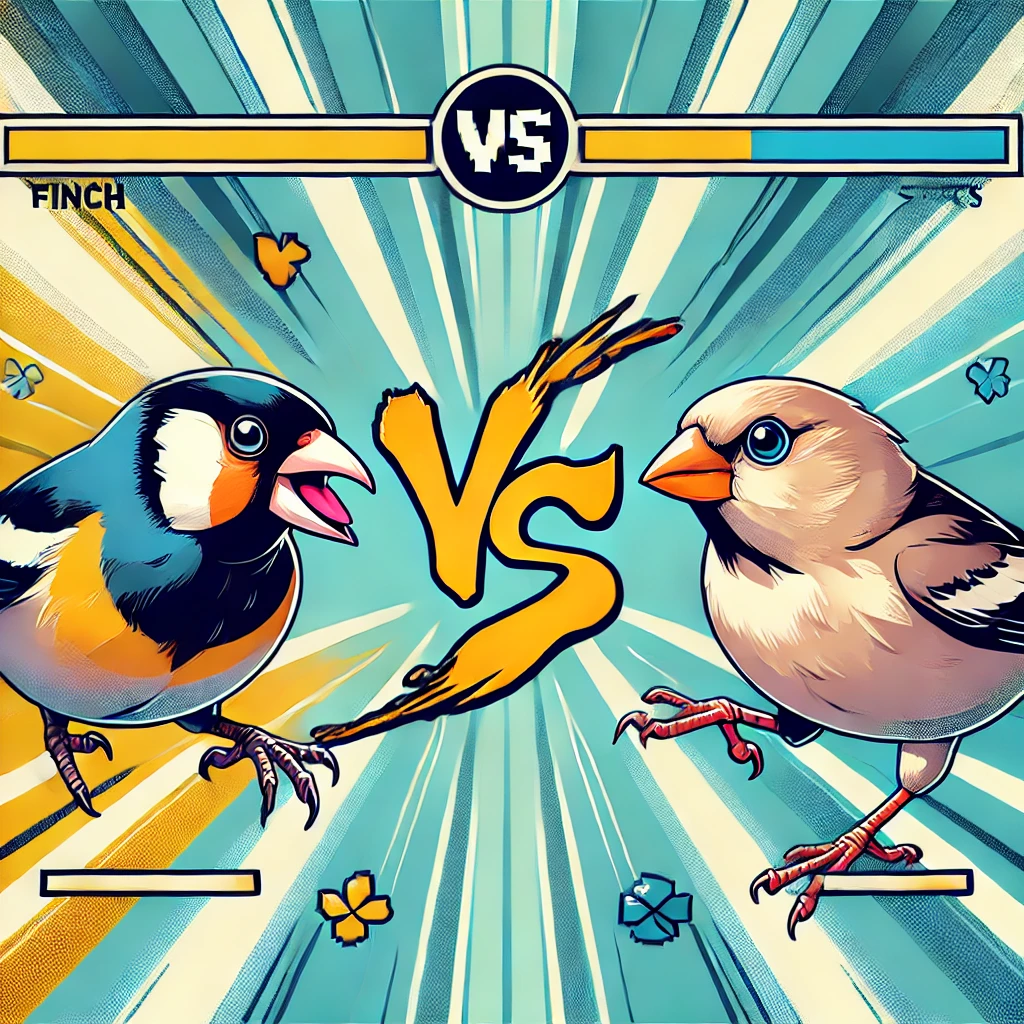
\includegraphics[width=0.7\textwidth,height=\textheight]{Modellering/figuren/vs_birds_ai.png}

}

\caption{Afbeelding gegenereerd met ChatGPT4-o}

\end{figure}

\hypertarget{leerdoelen-7}{%
\section{Leerdoelen}\label{leerdoelen-7}}

De leerdoelen voor dit hoofdstuk zijn:

\begin{itemize}
\tightlist
\item
  Begrijpen hoe intra- en interspecifieke interacties gemodelleerd
  kunnen worden
\item
  Mogelijke evenwichten in faseruimtes van competitie kunnen benoemen,
  en uitleggen wat de biologische intepretaties van deze evenwichten
  zijn
\item
  Een gegeven vectorveld afmaken en daarbij horende oplossingen schetsen
\end{itemize}

\hypertarget{competitie-binnen-en-tussen-soorten}{%
\section{Competitie binnen en tussen
soorten}\label{competitie-binnen-en-tussen-soorten}}

\textbf{Inter-specifieke competitie} is competitie tussen soorten, en
\textbf{intra-specifieke competitie} staat voor competitie binnen een
soort\footnote{Als je net als ik dit slecht kan onthouden, kun je de
  \textbf{Intratuin} als ezelsbruggetje gebruiken: ``in de tuin'' klinkt
  kloppend, maar ``tussen de tuin'' klinkt toch een beetje vreemd}. Als
twee soorten bijvoorbeeld voornamelijk hetzelfde voedsel eten (we
blijven nog even bij ecologie), zullen ze veel competitie om dat voedsel
hebben. Formeel zeggen we dan dat de niches van de soorten overlappen,
wat we bijvoorbeeld kunnen bepalen door precies te meten welk zaadjes
verschillende soorten vogels eten (Figuur~\ref{fig-zaadoverlap}). Hoe
meer de niches overlappen, hoe sterker de \textbf{inter-specifieke}
competitie.

\begin{Shaded}
\begin{Highlighting}[]
\NormalTok{n }\OtherTok{\textless{}{-}} \DecValTok{1}
\NormalTok{plot\_niche\_overlap }\OtherTok{\textless{}{-}} \ControlFlowTok{function}\NormalTok{(}\AttributeTok{mean1=}\SpecialCharTok{{-}}\DecValTok{1}\NormalTok{, }\AttributeTok{sd1=}\DecValTok{1}\NormalTok{, }\AttributeTok{mean2=}\DecValTok{1}\NormalTok{, }\AttributeTok{sd2=}\DecValTok{1}\NormalTok{)\{}
  \CommentTok{\# Define the range for the x{-}axis}
\NormalTok{  x\_range }\OtherTok{\textless{}{-}} \FunctionTok{seq}\NormalTok{(}\SpecialCharTok{{-}}\DecValTok{5}\NormalTok{, }\DecValTok{5}\NormalTok{, }\AttributeTok{length.out =} \DecValTok{1000}\NormalTok{)}
  
  \CommentTok{\# Calculate the densities}
\NormalTok{  density1 }\OtherTok{\textless{}{-}} \FunctionTok{dnorm}\NormalTok{(x\_range, }\AttributeTok{mean =}\NormalTok{ mean1, }\AttributeTok{sd =}\NormalTok{ sd1)}
\NormalTok{  density2 }\OtherTok{\textless{}{-}} \FunctionTok{dnorm}\NormalTok{(x\_range, }\AttributeTok{mean =}\NormalTok{ mean2, }\AttributeTok{sd =}\NormalTok{ sd2)}
  
  \CommentTok{\# Scale the densities to the same maximum height}
\NormalTok{  max\_height }\OtherTok{\textless{}{-}} \FloatTok{0.4}
\NormalTok{  density1\_scaled }\OtherTok{\textless{}{-}}\NormalTok{ density1 }\SpecialCharTok{/} \FunctionTok{max}\NormalTok{(density1) }\SpecialCharTok{*}\NormalTok{ max\_height}
\NormalTok{  density2\_scaled }\OtherTok{\textless{}{-}}\NormalTok{ density2 }\SpecialCharTok{/} \FunctionTok{max}\NormalTok{(density2) }\SpecialCharTok{*}\NormalTok{ max\_height}
\NormalTok{  overlap }\OtherTok{\textless{}{-}} \FunctionTok{pmin}\NormalTok{(density1\_scaled,density2\_scaled)}
  \CommentTok{\# Plot the first normal distribution}
  
  \FunctionTok{plot}\NormalTok{(x\_range, density1\_scaled, }\AttributeTok{type =} \StringTok{"l"}\NormalTok{, }
       \AttributeTok{axes=}\NormalTok{F, }\AttributeTok{xaxt=}\StringTok{\textquotesingle{}n\textquotesingle{}}\NormalTok{, }\AttributeTok{yaxt=}\StringTok{\textquotesingle{}n\textquotesingle{}}\NormalTok{,}\AttributeTok{yaxs=}\StringTok{"i"}\NormalTok{,}
       \AttributeTok{col =} \StringTok{"blue"}\NormalTok{, }\AttributeTok{lwd =} \DecValTok{2}\NormalTok{, }\AttributeTok{ylim =} \FunctionTok{c}\NormalTok{(}\DecValTok{0}\NormalTok{, max\_height}\SpecialCharTok{*}\FloatTok{1.1}\NormalTok{), }
       \AttributeTok{xlab =} \StringTok{""}\NormalTok{, }\AttributeTok{ylab =} \StringTok{""}\NormalTok{, }\AttributeTok{main =} \StringTok{""}\NormalTok{)}
  \FunctionTok{polygon}\NormalTok{(x\_range,overlap,}\AttributeTok{col=}\StringTok{"\#FF000033"}\NormalTok{,}\AttributeTok{border =} \ConstantTok{NA}\NormalTok{)}
  \FunctionTok{lines}\NormalTok{(x\_range, density1\_scaled, }\AttributeTok{col =} \StringTok{"blue"}\NormalTok{, }\AttributeTok{lwd =} \DecValTok{2}\NormalTok{)}
  \FunctionTok{lines}\NormalTok{(x\_range, density2\_scaled, }\AttributeTok{col =} \StringTok{"orange"}\NormalTok{, }\AttributeTok{lwd =} \DecValTok{2}\NormalTok{)}
  
  \FunctionTok{arrows}\NormalTok{(}\DecValTok{0}\NormalTok{,}\DecValTok{0}\NormalTok{,}\FloatTok{7.5}\NormalTok{,}\DecValTok{0}\NormalTok{,}\AttributeTok{xpd=}\ConstantTok{NA}\NormalTok{,}\AttributeTok{lwd=}\DecValTok{3}\NormalTok{,}\AttributeTok{length =} \FloatTok{0.1}\NormalTok{)}
  \FunctionTok{arrows}\NormalTok{(}\DecValTok{0}\NormalTok{,}\DecValTok{0}\NormalTok{,}\SpecialCharTok{{-}}\FloatTok{7.5}\NormalTok{,}\DecValTok{0}\NormalTok{,}\AttributeTok{xpd=}\ConstantTok{NA}\NormalTok{,}\AttributeTok{lwd=}\DecValTok{3}\NormalTok{,}\AttributeTok{length =} \FloatTok{0.1}\NormalTok{)}
  \FunctionTok{mtext}\NormalTok{(}\StringTok{"Kleine zaadjes"}\NormalTok{,}\DecValTok{1}\NormalTok{,}\AttributeTok{at=}\SpecialCharTok{{-}}\FloatTok{5.5}\NormalTok{,}\AttributeTok{cex=}\FloatTok{0.6}\NormalTok{)}
  \FunctionTok{mtext}\NormalTok{(}\StringTok{"Grote zaadjes"}\NormalTok{,}\DecValTok{1}\NormalTok{,}\AttributeTok{at=}\FloatTok{4.8}\NormalTok{,}\AttributeTok{cex=}\FloatTok{0.6}\NormalTok{)}
  \FunctionTok{text}\NormalTok{(}\SpecialCharTok{{-}}\DecValTok{10}\NormalTok{,}\FloatTok{0.6}\NormalTok{,}\FunctionTok{paste0}\NormalTok{(LETTERS[n],}\StringTok{\textquotesingle{})\textquotesingle{}}\NormalTok{),}\AttributeTok{font=}\DecValTok{2}\NormalTok{,}\AttributeTok{xpd=}\ConstantTok{NA}\NormalTok{)}
  
\NormalTok{  overlap\_pc }\OtherTok{\textless{}{-}} \FunctionTok{round}\NormalTok{(}\FunctionTok{sum}\NormalTok{(overlap)}\SpecialCharTok{/}\FunctionTok{sum}\NormalTok{(density1\_scaled),}\AttributeTok{digits=}\DecValTok{2}\NormalTok{)}\SpecialCharTok{*}\DecValTok{100}
\CommentTok{\#   title(main=paste0("N1 heeft ", }
\CommentTok{\#                     round(sum(overlap)/sum(density1\_scaled),2)*100,"\%",}
\CommentTok{\#                     " overlap met N2\textbackslash{}n",}
\CommentTok{\#                     "N2 heeft ", }
\CommentTok{\#                     round(sum(overlap)/sum(density2\_scaled),2)*100,"\%",}
\CommentTok{\#                     " overlap met N1"),line = 0.5,cex.main=0.7)}
\CommentTok{\#   n \textless{}\textless{}{-} n + 1}
\NormalTok{\}}
\FunctionTok{par}\NormalTok{(}\AttributeTok{mfrow=}\FunctionTok{c}\NormalTok{(}\DecValTok{1}\NormalTok{,}\DecValTok{1}\NormalTok{),}\AttributeTok{mar=}\FunctionTok{c}\NormalTok{(}\DecValTok{4}\NormalTok{,}\DecValTok{4}\NormalTok{,}\DecValTok{0}\NormalTok{,}\DecValTok{4}\NormalTok{))}
\FunctionTok{plot\_niche\_overlap}\NormalTok{()}
\end{Highlighting}
\end{Shaded}

\begin{figure}[H]

{\centering 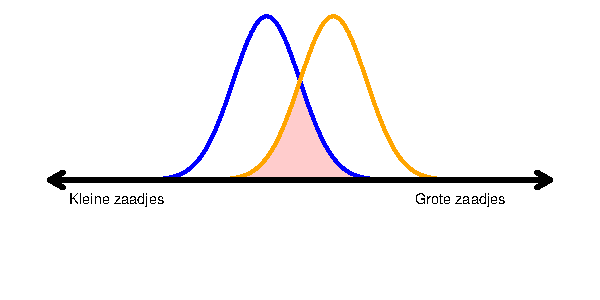
\includegraphics{Modellering/ecoevo_competitie_files/figure-pdf/fig-zaadoverlap-1.pdf}

}

\caption{\label{fig-zaadoverlap}Als twee vogelsoorten verschillende
voorkeur voor zaadgrootte hebben, zullen we competitie hebben om de
zaadjes waar ze overlappen.}

\end{figure}

De niche overlap binnen een soort is eigenlijk per definitie 100\%. Het
is daarom redelijk om aan te nemen dat de competitie om voedsel binnen
een soort (intra-specifieke competitie) sterker dan de inter-specifieke
competitie om voedsel. Echter kan \textbf{intra-specifieke competitie}
ook door andere biologische processen teweeg gebracht worden. Zo kunnen
bijvoorbeeld haviken uilen aanvallen om hen uit de beste jachtgebieden
te verdrijven, of produceren veel schimmels toxines om bacteriën te
onderdrukken. Zodoende kan het toch zijn dat de intra-specifieke
competitie de overhand speelt, afhankelijk van de situatie. Hoe hebben
de twee bovengenoemde processen precies invloed om het wel/niet kunnen
samenleven van soorten? Dit gaan we bestuderen met het
\textbf{Lotka-Volterra competitie} model (vergelijkbaar maar niet
hetzelfde als het Lotka-Volterra predator-prooi model).

\hypertarget{lotka-volterra-competitie}{%
\section{Lotka-Volterra competitie}\label{lotka-volterra-competitie}}

Laten we aannemen dat er twee populaties bestaan die beide logistisch
groeien, genaamd \(N_1\) en \(N_2\):

\begin{align*}
\mathchoice{\frac{\mathrm{d}N_1}
{\mathrm{d}t}}{\mathrm{d}N_1/\mathrm{d}t}
{\mathrm{d}N_1/\mathrm{d}t}
{\mathrm{d}N_1/\mathrm{d}t} &= rN_1(1-\frac{N_1}{K}) \\
\mathchoice{\frac{\mathrm{d}N_2}
{\mathrm{d}t}}{\mathrm{d}N_2/\mathrm{d}t}
{\mathrm{d}N_2/\mathrm{d}t}
{\mathrm{d}N_2/\mathrm{d}t} &= rN_2(1-\frac{N_2}{K})
\end{align*}

Let op! De bovenstaande ODEs beschrijven géén interacties tussen de
soorten: \(N_1\) bevat alleen \(N_1\), en \(N_2\) bevat alleen \(N_2\).
Biologisch betekent dat dus dat de groei van \(N_1\) niet beïnvloed
wordt door de aanwezigheid van \(N_2\), en \emph{vice versa}. Er is dus
wel sprake van \textbf{intra}specifieke competitie (de soorten hebben
competitie met zichzelf), maar niet van \textbf{inter}specifieke
competitie. Om ook interspecifieke comptitie te modelleren, kunnen we
aannemen dat de dichtheid van beide soorten (\(N_1\) + \(N_2\)) bepaalt
of het draagvlak is bereikt (en of er dus nog groei mogelijk is):

\begin{align*}
\mathchoice{\frac{\mathrm{d}N_1}
{\mathrm{d}t}}{\mathrm{d}N_1/\mathrm{d}t}
{\mathrm{d}N_1/\mathrm{d}t}
{\mathrm{d}N_1/\mathrm{d}t} &= rN_1(1-\frac{N_1+N_2}{K}) \\
\mathchoice{\frac{\mathrm{d}N_2}
{\mathrm{d}t}}{\mathrm{d}N_2/\mathrm{d}t}
{\mathrm{d}N_2/\mathrm{d}t}
{\mathrm{d}N_2/\mathrm{d}t} &= rN_2(1-\frac{N_1+N_2}{K})
\end{align*}

Beide populaties hebben nu een gedeeld draagvlak (\(K\)). Dit is
biologisch goed te verdedigen: deze wordt bepaald door de hoeveelheid
voedsel of ruimte. Echter ondervinden beide populaties precies dezelfde
dichtheidseffecten. Maar wellicht heeft soort 1 sterkere competitie met
``zichzelf'' (intra), en soort 2 sterke competitie met ``de ander''
(inter). Om dit te kunnen bestuderen, introduceren we een set van vier
nieuwe parameters toe die de intra- en interspecifieke competitie
schalen:

\begin{align*}
\mathchoice{\frac{\mathrm{d}N_1}
{\mathrm{d}t}}{\mathrm{d}N_1/\mathrm{d}t}
{\mathrm{d}N_1/\mathrm{d}t}
{\mathrm{d}N_1/\mathrm{d}t} &= rN_1(1-\frac{c_{11}N_1+c_{12}N_2}{K}) \\
\mathchoice{\frac{\mathrm{d}N_2}
{\mathrm{d}t}}{\mathrm{d}N_2/\mathrm{d}t}
{\mathrm{d}N_2/\mathrm{d}t}
{\mathrm{d}N_2/\mathrm{d}t} &= rN_2(1-\frac{c_{22}N_2+c_{21}N_1}{K})
\end{align*}

Hierbij schalen \(c_{11}\) en \(c_{22}\) de intraspecifieke competitie
voor respectievelijk soort 1 en 2, \(c_{12}\) de competitie die soort 1
van soort 2 ondervindt, en \(c_{21}\) de competitie die soort 2 van
soort 1 ondervindt. Laten we het aantal parameters beperken door aan te
nemen dat \(K=1\), waardoor we deze kunnen weglaten uit de vergelijking.
Als we \(N1\) blauw kleuren, en \(N2\) oranje, dan wordt ons systeem:

\begin{align*}
\color{blue} \mathchoice{\frac{\mathrm{d}N_1}
{\mathrm{d}t}}{\mathrm{d}N_1/\mathrm{d}t}
{\mathrm{d}N_1/\mathrm{d}t}
{\mathrm{d}N_1/\mathrm{d}t} &= r\textcolor{blue}{N_1}(1 - c_{11}\textcolor{blue}{N_1} - c_{12}\textcolor{orange}{N_2})\\
\color{orange}\mathchoice{\frac{\mathrm{d}N_2}
{\mathrm{d}t}}{\mathrm{d}N_2/\mathrm{d}t}
{\mathrm{d}N_2/\mathrm{d}t}
{\mathrm{d}N_2/\mathrm{d}t} &= r\textcolor{orange}{N_2}(1 - c_{22}\textcolor{orange}{N_2} - c_{21}\textcolor{blue}{N_1})
\end{align*}

Om te kunnen onderzoeken of twee soorten kunnen samenleven, en onder
welke voorwaarden, kunnen we weer de faseruimte analyseren. In het
vorige hoofdstuk heb je geleerd hoe je dit eenvoudig met R zou kunnen
doen. Echter is er ook een belangrijk voordeel aan het zelf schetsen van
de faseruimte: we weten dan precies welke parameters bepalen hoe de
nullclines liggen. Bovendien ontwikkel je door hiermee te oefenen een
beter gevoel voor deze dynamische systemen. Daarom staat in
(\textbf{tip-odesschetsen?}) een uitgebreid stappenplan voor het zelf
tekenen van een faseruimte.

\begin{tcolorbox}[enhanced jigsaw, coltitle=black, breakable, bottomtitle=1mm, opacityback=0, colback=white, rightrule=.15mm, title=\textcolor{quarto-callout-tip-color}{\faLightbulb}\hspace{0.5em}{Algemeen stappenplan voor het schetsen van faseruimtes.}, bottomrule=.15mm, toprule=.15mm, left=2mm, colframe=quarto-callout-tip-color-frame, toptitle=1mm, opacitybacktitle=0.6, titlerule=0mm, colbacktitle=quarto-callout-tip-color!10!white, leftrule=.75mm, arc=.35mm]

Stel, we analyseren een 2D ODE systeem bestaande uit variable \(A\) en
\(B\):

\begin{enumerate}
\def\labelenumi{\arabic{enumi}.}
\tightlist
\item
  Teken een assenstelsen met één populatie op de x-as, en de ander op de
  y-as. We zetten bijvoorbeeld A op de y-as en B op de x-as.
\item
  Vind de nullcline(s) voor A. Hiervoor los je
  \(\mathchoice{\frac{\mathrm{d}A}
  {\mathrm{d}t}}{\mathrm{d}A/\mathrm{d}t}
  {\mathrm{d}A/\mathrm{d}t}
  {\mathrm{d}A/\mathrm{d}t}=0\) op. Je kan een aantal verschillende
  typen nullclines vinden:

  \begin{itemize}
  \tightlist
  \item
    \(A=0\), wat gebeurt als elke term \(A\) bevat. Voor groeimodellen
    komt deze nullcline vaak (maar niet altijd!) voor.
  \item
    \(A=C\), een \emph{horizontale} lijn bij een niet-triviale
    hoeveelheid \(A\).
  \item
    \(B=C\), een \emph{verticale} lijn bij een niet-triviale hoeveelheid
    \(B\).
  \item
    \(A=f(B)\) of \(B=f(A)\), wat gebeurt als je beide onbekenden (\(A\)
    en \(B\)) overhoudt. In dit geval is het vaak makkelijk om de zoeken
    naar een functie die in je assenstelsel een functie y=f(x) geeft. In
    dit geval is dus \(A=f(B)\) prettiger, want we hadden ervoor gekozen
    \(A\) op de y-as te zetten.
  \end{itemize}
\item
  Vind ook de nullclines voor B. Als je wederom twee onbekenden
  overhoudt, zoek dan \(A=f(B)\) zodat je die makkelijk kan schetsen.
\item
  Teken de nullclines. Zorg dat je weet waar de nullclines (eventueel)
  de x- en y-as snijden, want dit kan belangrijk zijn om te bepalen of
  de nullclines elkaar snijden.

  \begin{itemize}
  \tightlist
  \item
    Snijpunten met de y-as vind je door \(x=0\) in de vullen.
  \item
    Snijpunten met de x-as vindt je door \(f(x)=0\) op te lossen.
  \end{itemize}
\item
  Neem een extreme waarde in de faseruimte, en ga in de oorspronkelijke
  ODEs op zoek naar termen met hoge machten (kwadratische termen zoals
  (\(A^2\), \(B^2\), of \(AB\), of misschien zelfs \(A^3\), \(B^4\),
  \emph{etc.}). De termen met de hoogste macht hebben altijd de overhand
  bij extreme waarden. Dat wil zeggen: deze termen zijn extra klein als
  de variabelen klein zijn, en extra groot als de variabelen groot zijn.
  Zo kun je bepalen wie zal groeien/krimpen.
\item
  Teken pijltjes in deze hoek van de faseruimte om te richting van
  verandering aan te geven.
\item
  Vul de rest van het vectorveld in. De \(A\) en \(B\) nullclines geven
  aan waar het pijltje van richting verandert (respectievelijk voor
  \(A\) en \(B\))
\item
  Kies de begintoetsand waarin je geïnteresseerd bent. Schets een
  trajectory die de richtingen van het vectorveld volgt. Dit hoeft niet
  precies te kloppen.
\item
  Schets eventueel de oplossing die hierbij hoort.
\end{enumerate}

\end{tcolorbox}

\hypertarget{faseruimte-van-het-competitiemodel}{%
\section{Faseruimte van het
competitiemodel}\label{faseruimte-van-het-competitiemodel}}

We volgen het hierboven genoemde stappenplan voor de analyse van ODEs,
en gaan een faseruimte maken van het competitiemodel zoals eerder
besproken:

\begin{equation}\protect\hypertarget{eq-soorten}{}{
\color{blue} \mathchoice{\frac{\mathrm{d}N_1}
{\mathrm{d}t}}{\mathrm{d}N_1/\mathrm{d}t}
{\mathrm{d}N_1/\mathrm{d}t}
{\mathrm{d}N_1/\mathrm{d}t} = r\textcolor{blue}{N_1}(1 - c_{11}\textcolor{blue}{N_1} - c_{12}\textcolor{orange}{N_2})\\
\color{orange}\mathchoice{\frac{\mathrm{d}N_2}
{\mathrm{d}t}}{\mathrm{d}N_2/\mathrm{d}t}
{\mathrm{d}N_2/\mathrm{d}t}
{\mathrm{d}N_2/\mathrm{d}t} = r\textcolor{orange}{N_2}(1 - c_{22}\textcolor{orange}{N_2} - c_{21}\textcolor{blue}{N_1})
}\label{eq-soorten}\end{equation}

Zoals gezegd is het handig om eerst te kiezen wat we op straks op de x-
en y-as gaan zetten (deze keuze heeft geen invloed op het model zelf,
alleen op de visualisatie). Laten we ervoor kiezen om \(N_1\) op de x-as
te zetten, en \(N_2\) op de y-as. We stellen beide ODEs gelijk aan 0, en
gaan nullclines bepalen:

\begin{align*}
\color{blue} \mathchoice{\frac{\mathrm{d}N_1}
{\mathrm{d}t}}{\mathrm{d}N_1/\mathrm{d}t}
{\mathrm{d}N_1/\mathrm{d}t}
{\mathrm{d}N_1/\mathrm{d}t} &= r\textcolor{blue}{N_1}(1 - c_{11}\textcolor{blue}{N_1} - c_{12}\textcolor{orange}{N_2}) = 0  \quad \text{als...} \\
\textcolor{blue}{N_1} &= 0 \quad \text{of...} \\
1 - c_{11}\textcolor{blue}{N_1} - c_{12}\textcolor{orange}{N_2} &= 0 \\
 \textcolor{orange}{N_2} &= \frac{1 - c_{11}\textcolor{blue}{N_1}}{c_{12}}
\end{align*}

Let op dat dit beide nullclines zijn voor {N1}. Met andere woorden:
hoewel de tweede nullcline uitgedrukt is als \(N_2=f(N_1)\), wordt dit
straks een {blauwe} nullcline. We hadden deze nullcline ook kunnen
uitdrukken als \(N_1=f(N_2)\), maar omdat \(N_2\) op de y-as staat, is
die laatste keuze wat minder fijn schetsen.

Op dezelfde manier kunnen we ook de \(N_2\) ({oranje}) nullclines
vinden:

\begin{align*}
\textcolor{orange}{N_2} &= 0 \quad \text{of...} \\
\textcolor{orange}{N_2} &= \frac{1 - c_{21}\textcolor{blue}{N_1}}{c_{22}}
\end{align*}

We vinden dus ook twee nullclines voor \(N_2\). We vinden wederom een
nullcline voor een populatiegrootte van 0 (een populatie die niet
bestaat kan ook niet groeien), en een nullcline die we uitdrukken als
\(N_2=f(N_1)\), zodat we dit kunnen schetsen in de vorm \(y=f(x)\).

De twee ``triviale'' nullclines (dus \(N_1=0\) en \(N_2=0\)) zijn
simpelweg lijnen die op de assen liggen. De andere twee nullclines zijn
functies die lineair afnemen met \(N_1\), maar let op, er staan andere
parameters in de vergelijkingen. Om precies te bepalen hoe deze rechte
lijnen lopen, moeten we hun snijpunten met de x- en de y-as bepalen. {De
nullcline van \(N_1\)} snijdt de y-as wanneer \(N_1=0\), dus bij
\(N_2=\frac{1}{c_{12}}\), en de x-as bij
\(\frac{1 - c_{11}N_1}{c_{12}}=0\), wat alleen 0 is als de teller 0 is,
dus als \(N1=\frac{1}{c_{11}}\). Vergelijkbaar, snijdt {de nullcline van
\(N_2\)} de y-as bij \(N_2=\frac{1}{c_{22}}\) en de x-as bij
\(N_1=\frac{1}{c_{21}}\).

Om precies te weten hoe deze lijnen in de faseruimte liggen, moeten we
keuzes maken over de parameters. Als we bijvoorbeeld aannemen dat
interspecifieke competitie zwakker is dan intraspecifieke competitie
(\(c_{12}\) en \(c_{21}\) zijn kleiner dan \(c_{11}\) en \(c_{22}\)),
dan liggen de nullclines zoals weergegeven in
(Figuur~\ref{fig-competition_nullclines-1}). Om ook het vectorveld te
bepalen, kijken we altijd naar extreme waarden (heel veel of weinig van
beide populaties). Voor deze vergelijkingen komen we heel ver met alleen
intuïtie: als beide soorten heel abundant zijn, kunnen ze alleen maar
afnemen. Ook in de vergelijkingen zie je dit terug: als je de ODEs
uitvermenigvuldigd zijn er kwadratische termen voor de competitie,
terwijl de groei lineair toeneemt. Als de populaties dus heel groot
zijn, zal competitie de overhand spelen, en de populaties dus afnemen.
Beide manieren tonen dus aan dat het vectorveld rechtsbovenin naar
links/onder wijst. De andere punten van het vectorveld kunnen we
simpelweg afmaken door de pijltjes om te laten klappen als je over een
nullcline gaat. Gaan we over een \(N_1\) nullcline dan klapt de x-as om
(want \(N_1\) staat op de x-as), en gaan we over een \(N_2\) nullcline
dan klapt de y-as om. Omdat alle pijltjes naar het snijpunt wijzen
(Figuur~\ref{fig-competition_nullclines-2}), weten we dat het evenwicht
op dit punt stabiel is.

\begin{figure}

\begin{minipage}[t]{0.50\linewidth}

{\centering 

\raisebox{-\height}{

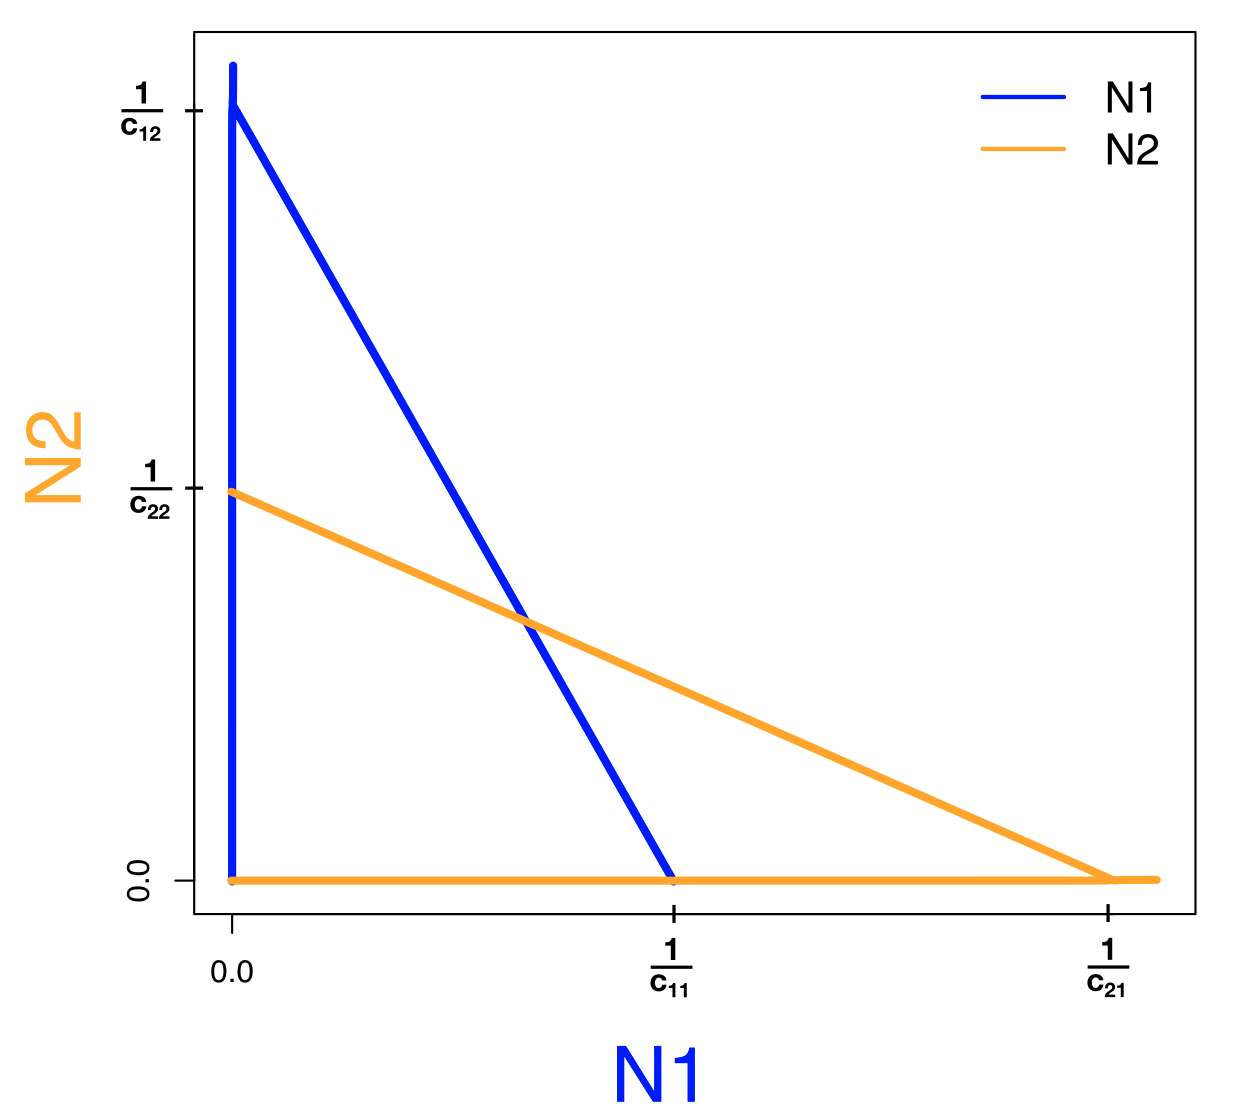
\includegraphics{Modellering/figuren/nullclines_competition.png}

}

}

\subcaption{\label{fig-competition_nullclines-1}\textbf{?(caption)}}
\end{minipage}%
%
\begin{minipage}[t]{0.50\linewidth}

{\centering 

\raisebox{-\height}{

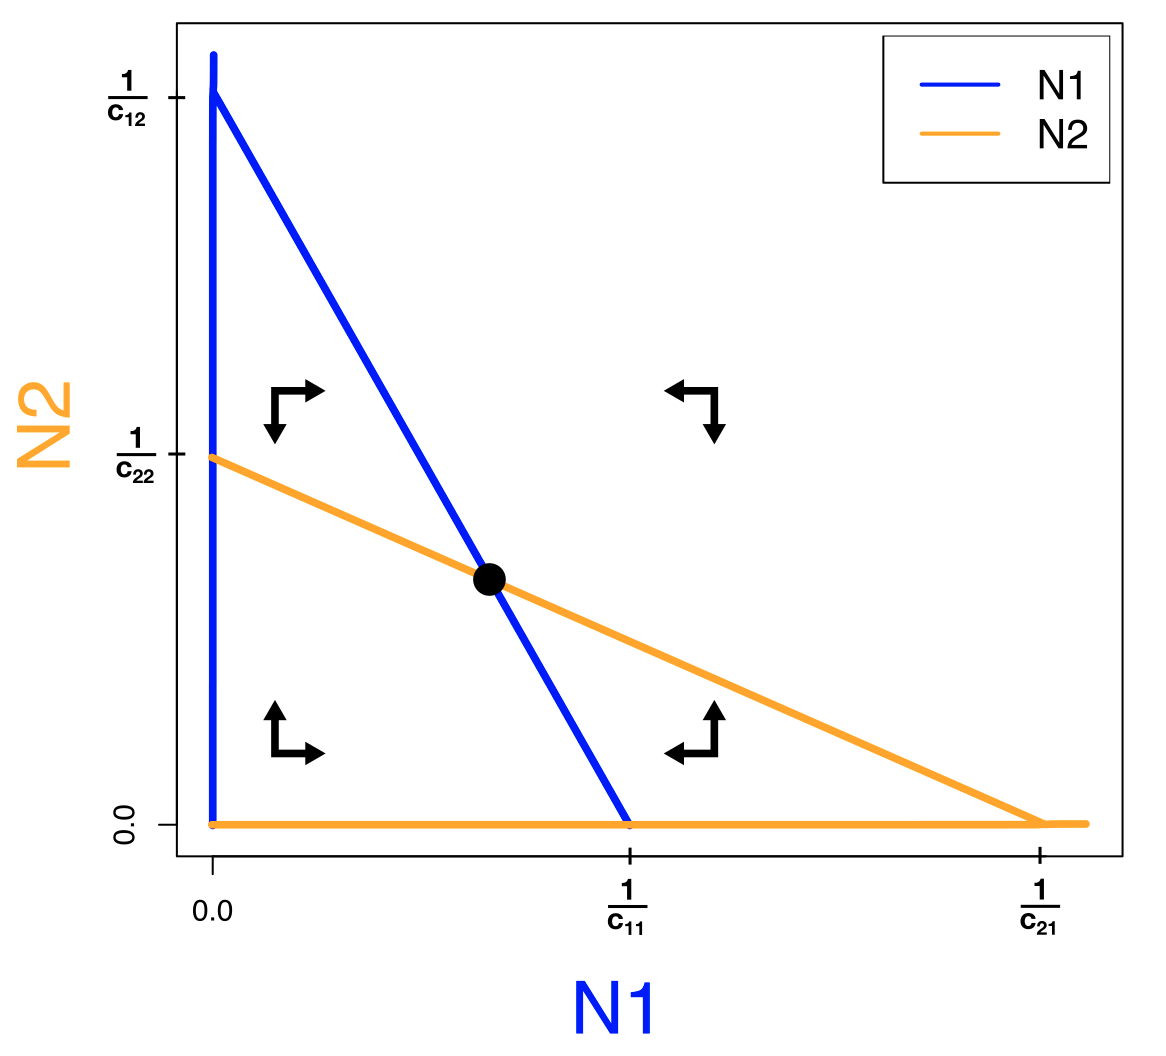
\includegraphics{Modellering/figuren/nullclines_competition_vect.png}

}

}

\subcaption{\label{fig-competition_nullclines-2}\textbf{?(caption)}}
\end{minipage}%

\caption{\label{fig-competition_nullclines}Faseruimte voor het
Lotka-Volterra competitie model, aangenomen dat competitie binnen
soorten sterker is dan competitie tussen soorten (\(c_{12}\) en
\(c_{21}\) zijn kleiner dan \(c_{11}\) en \(c_{22}\)).}

\end{figure}

\begin{exercise}[Sterkere intraspecifieke
competitie]\protect\hypertarget{exr-compofexcl}{}\label{exr-compofexcl}

Hierboven hebben we nullclines geschetst van het competitiemodel, onder
de aannamen dat interspecifieke competitie sterker is dan
intraspecifieke competitie (\(c_{12}\) en \(c_{21}\) zijn kleiner dan
\(c_{11}\) en \(c_{22}\)). Beginnende vanuit deze opstellen: stel dat
\(N_2\) steeds sterkere competitie krijgt met \(N_1\).

\begin{enumerate}
\def\labelenumi{\alph{enumi}.}
\tightlist
\item
  Welke parameter gaat er veranderen? \emph{c21 wordt groter}
\item
  Welke nullcline in deze faseruimte zal verschuiven? \emph{ANTWOORD: de
  oranje lijn: het snijpunt van de oranje lijn met de x-as schuift naar
  links}. Als deze verschuiving doorzet, zullen de parameters op een
  gegeven moment niet meer snijden.
\item
  Vanaf wel punt gebeurt dit? \emph{als c21 groter is dan c11}
\item
  Schets het vectorveld in de situatie dat de nullclines niet snijden,
  en teken een trajectorie om aan te geven wat er zal gebeuren als je
  met veel van beide soorten begint. \emph{N1 gaat winnen}
\end{enumerate}

\end{exercise}

\hypertarget{coexistentie-of-exclusie}{%
\section{Coexistentie of exclusie?}\label{coexistentie-of-exclusie}}

Afhankelijk van de parameters zien we dat de nullclines van het
Lotka-Volterra competitie model anders kunnen liggen. Laten we
\texttt{Grind} gebruiken om het bovenstaande model verder te analyseren.
We nemen eerst aan dat interspecifieke competitie sterker is dan
intraspecifieke competitie.

\begin{Shaded}
\begin{Highlighting}[]
\CommentTok{\#Laad het grind.R{-}script in}
\FunctionTok{source}\NormalTok{(}\StringTok{"https://tbb.bio.uu.nl/rdb/grindR/grind.R"}\NormalTok{)}
\end{Highlighting}
\end{Shaded}

\begin{verbatim}
Warning: package 'deSolve' was built under R version 4.4.2
\end{verbatim}

\begin{verbatim}
Warning: package 'FME' was built under R version 4.4.2
\end{verbatim}

\begin{Shaded}
\begin{Highlighting}[]
\CommentTok{\# Definitie van model. }
\NormalTok{model }\OtherTok{\textless{}{-}} \ControlFlowTok{function}\NormalTok{(t, state, parms) \{}
  \FunctionTok{with}\NormalTok{(}\FunctionTok{as.list}\NormalTok{(}\FunctionTok{c}\NormalTok{(state,parms)), \{}
\NormalTok{    dN1 }\OtherTok{\textless{}{-}}\NormalTok{ r}\SpecialCharTok{*}\NormalTok{N1}\SpecialCharTok{*}\NormalTok{(}\DecValTok{1}\SpecialCharTok{{-}}\NormalTok{c11}\SpecialCharTok{*}\NormalTok{N1}\SpecialCharTok{{-}}\NormalTok{c12}\SpecialCharTok{*}\NormalTok{N2)}
\NormalTok{    dN2 }\OtherTok{\textless{}{-}}\NormalTok{ r}\SpecialCharTok{*}\NormalTok{N2}\SpecialCharTok{*}\NormalTok{(}\DecValTok{1}\SpecialCharTok{{-}}\NormalTok{c22}\SpecialCharTok{*}\NormalTok{N2}\SpecialCharTok{{-}}\NormalTok{c21}\SpecialCharTok{*}\NormalTok{N1)}
    \FunctionTok{return}\NormalTok{(}\FunctionTok{list}\NormalTok{(}\FunctionTok{c}\NormalTok{(dN1, dN2)))  }
\NormalTok{  \}) }
\NormalTok{\}  }


\NormalTok{p }\OtherTok{\textless{}{-}} \FunctionTok{c}\NormalTok{(}\AttributeTok{r=}\DecValTok{1}\NormalTok{,}\AttributeTok{c11=}\DecValTok{2}\NormalTok{,}\AttributeTok{c22=}\DecValTok{2}\NormalTok{,}\AttributeTok{c12=}\DecValTok{1}\NormalTok{,}\AttributeTok{c21=}\DecValTok{1}\NormalTok{)  }\CommentTok{\#parameters}
\NormalTok{s }\OtherTok{\textless{}{-}} \FunctionTok{c}\NormalTok{(}\AttributeTok{N1=}\FloatTok{0.01}\NormalTok{,}\AttributeTok{N2=}\FloatTok{0.001}\NormalTok{) }\CommentTok{\# kleine begin{-}dichtheden}

\NormalTok{colors[}\DecValTok{1}\NormalTok{] }\OtherTok{=} \StringTok{"blue"}
\NormalTok{colors[}\DecValTok{2}\NormalTok{] }\OtherTok{=} \StringTok{"orange"}
\FunctionTok{par}\NormalTok{(}\AttributeTok{mfrow=}\FunctionTok{c}\NormalTok{(}\DecValTok{1}\NormalTok{,}\DecValTok{2}\NormalTok{)) }\CommentTok{\# maak twee plot{-}ruimtes}
\FunctionTok{plane}\NormalTok{(}\AttributeTok{vector=}\NormalTok{T,}\AttributeTok{grid=}\DecValTok{3}\NormalTok{) }\CommentTok{\# faseruimte }
\FunctionTok{run}\NormalTok{(}\AttributeTok{traject=}\NormalTok{F,}\AttributeTok{tstep=}\FloatTok{0.1}\NormalTok{,}\AttributeTok{col=}\StringTok{"black"}\NormalTok{,}\AttributeTok{tmax=}\DecValTok{50}\NormalTok{) }\CommentTok{\# numerieke oplossing}
\FunctionTok{mtext}\NormalTok{(}\StringTok{"LV competitie met sterke intraspecifieke competitie"}\NormalTok{, }\AttributeTok{cex=}\FloatTok{1.2}\NormalTok{,}\AttributeTok{font=}\DecValTok{2}\NormalTok{,}\AttributeTok{side =} \DecValTok{3}\NormalTok{, }\AttributeTok{line =} \SpecialCharTok{{-}}\DecValTok{3}\NormalTok{, }\AttributeTok{outer =} \ConstantTok{TRUE}\NormalTok{)}
\end{Highlighting}
\end{Shaded}

\begin{figure}[H]

{\centering 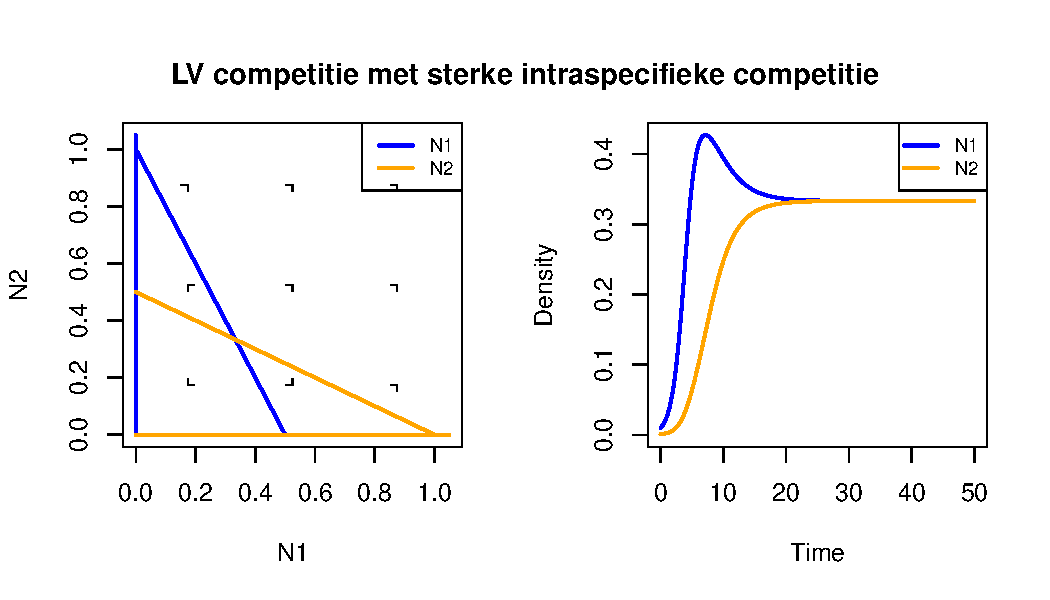
\includegraphics{Modellering/ecoevo_competitie_files/figure-pdf/unnamed-chunk-2-1.pdf}

}

\end{figure}

Het bovenstaande Grind-script bevestigt wat we net met pen-en-papier al
hebben aangetoond: twee soorten kunnen samenleven wanneer er sterke
intraspecifieke competitie is. Het evenwicht waar beide soorten
voorkomen is dus een \textbf{attractor} van het systeem. Je zou je deze
attractor kunnen voorstellen als een kuil waar een balletje door de
zwaartekracht heen zal rollen (zie linkerzijde van
Figuur~\ref{fig-attractorlandscapes}). Tenzij één van de soorten vanaf
het begin afwezig is, krijgen we dus altijd coexistentie
(\emph{coexistence}).

\begin{figure}

{\centering 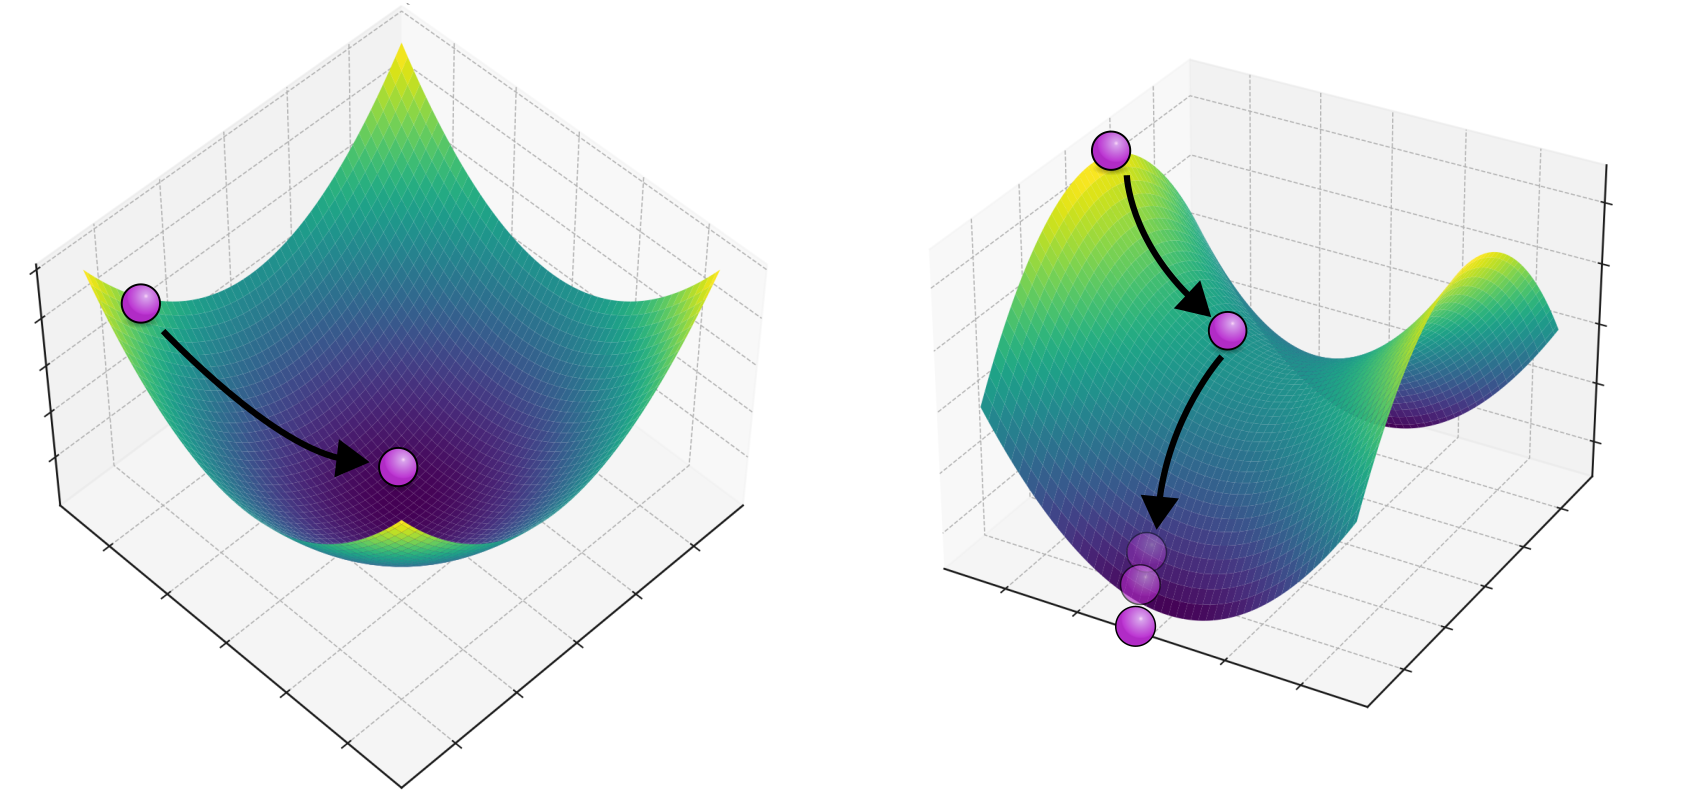
\includegraphics{Modellering/figuren/attractor_landscapes.png}

}

\caption{\label{fig-attractorlandscapes}CAPTION TODO}

\end{figure}

Omdat we nu ons R-script klaar hebben liggen, is het triviaal om deze
aan te passen voor een scenario waar de twee soorten juist hele sterke
\textbf{inter}specifieke competitie hebben, bijvoorbeeld wanneer twee
bacterien toxines produceren om elkaar te inhiberen:

\begin{Shaded}
\begin{Highlighting}[]
\CommentTok{\# Laad het grind.R{-}script in}
\FunctionTok{source}\NormalTok{(}\StringTok{"https://tbb.bio.uu.nl/rdb/grindR/grind.R"}\NormalTok{)}

\CommentTok{\# Definitie van model. }
\NormalTok{model }\OtherTok{\textless{}{-}} \ControlFlowTok{function}\NormalTok{(t, state, parms) \{}
  \FunctionTok{with}\NormalTok{(}\FunctionTok{as.list}\NormalTok{(}\FunctionTok{c}\NormalTok{(state,parms)), \{}
\NormalTok{    dN1 }\OtherTok{\textless{}{-}}\NormalTok{ r}\SpecialCharTok{*}\NormalTok{N1}\SpecialCharTok{*}\NormalTok{(}\DecValTok{1}\SpecialCharTok{{-}}\NormalTok{c11}\SpecialCharTok{*}\NormalTok{N1}\SpecialCharTok{{-}}\NormalTok{c12}\SpecialCharTok{*}\NormalTok{N2)}
\NormalTok{    dN2 }\OtherTok{\textless{}{-}}\NormalTok{ r}\SpecialCharTok{*}\NormalTok{N2}\SpecialCharTok{*}\NormalTok{(}\DecValTok{1}\SpecialCharTok{{-}}\NormalTok{c22}\SpecialCharTok{*}\NormalTok{N2}\SpecialCharTok{{-}}\NormalTok{c21}\SpecialCharTok{*}\NormalTok{N1)}
    \FunctionTok{return}\NormalTok{(}\FunctionTok{list}\NormalTok{(}\FunctionTok{c}\NormalTok{(dN1, dN2)))  }
\NormalTok{  \}) }
\NormalTok{\}  }


\NormalTok{p }\OtherTok{\textless{}{-}} \FunctionTok{c}\NormalTok{(}\AttributeTok{r=}\DecValTok{1}\NormalTok{,}\AttributeTok{c11=}\DecValTok{1}\NormalTok{,}\AttributeTok{c22=}\DecValTok{1}\NormalTok{,}\AttributeTok{c12=}\DecValTok{2}\NormalTok{,}\AttributeTok{c21=}\DecValTok{2}\NormalTok{)  }\CommentTok{\#parameters}
\NormalTok{s }\OtherTok{\textless{}{-}} \FunctionTok{c}\NormalTok{(}\AttributeTok{N1=}\FloatTok{0.01}\NormalTok{,}\AttributeTok{N2=}\FloatTok{0.001}\NormalTok{) }\CommentTok{\# kleine begin{-}dichtheden}

\NormalTok{colors[}\DecValTok{1}\NormalTok{] }\OtherTok{=} \StringTok{"blue"}
\NormalTok{colors[}\DecValTok{2}\NormalTok{] }\OtherTok{=} \StringTok{"orange"}
\FunctionTok{par}\NormalTok{(}\AttributeTok{mfrow=}\FunctionTok{c}\NormalTok{(}\DecValTok{1}\NormalTok{,}\DecValTok{2}\NormalTok{)) }\CommentTok{\# maak twee plot{-}ruimtes}
\FunctionTok{plane}\NormalTok{(}\AttributeTok{vector=}\NormalTok{T,}\AttributeTok{grid=}\DecValTok{3}\NormalTok{) }\CommentTok{\# faseruimte }
\FunctionTok{run}\NormalTok{(}\AttributeTok{traject=}\NormalTok{F,}\AttributeTok{tstep=}\FloatTok{0.1}\NormalTok{,}\AttributeTok{col=}\StringTok{"black"}\NormalTok{,}\AttributeTok{tmax=}\DecValTok{50}\NormalTok{) }\CommentTok{\# numerieke oplossing}
\FunctionTok{mtext}\NormalTok{(}\StringTok{"LV competitie met sterke interspecifieke competitie"}\NormalTok{, }\AttributeTok{cex=}\FloatTok{1.2}\NormalTok{,}\AttributeTok{font=}\DecValTok{2}\NormalTok{,}\AttributeTok{side =} \DecValTok{3}\NormalTok{, }\AttributeTok{line =} \SpecialCharTok{{-}}\DecValTok{3}\NormalTok{, }\AttributeTok{outer =} \ConstantTok{TRUE}\NormalTok{)}
\end{Highlighting}
\end{Shaded}

\begin{figure}[H]

{\centering 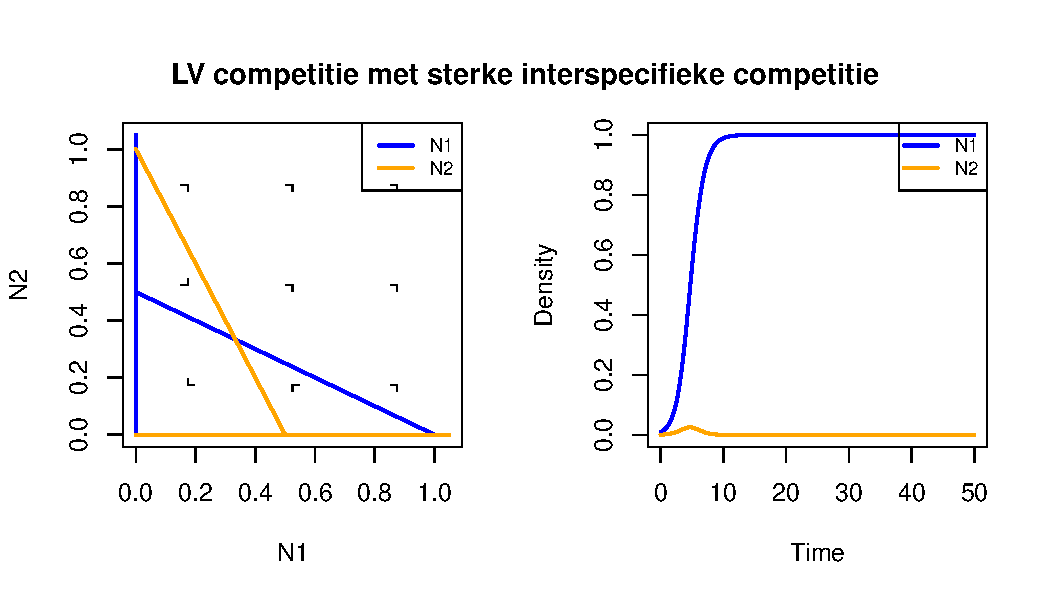
\includegraphics{Modellering/ecoevo_competitie_files/figure-pdf/unnamed-chunk-3-1.pdf}

}

\end{figure}

Zoals je ziet heeft deze parameterverandering het vectorveld verandert:
waar eerst \textbf{alle} pijltjes naar het evenwicht in het midden
wezen, wijzen nu slechts twee van de vier pijltjes naar het evenwicht.
De andere twee wijzen er juist van weg. Dit type evenwicht heet een
zadelpunt (\emph{saddle point}).

Als we ons weer een balletje voorstellen dat naar beneden rolt, zal dit
er uitzien zoals de rechterzijde van
Figuur~\ref{fig-attractorlandscapes}. Of het balletje naar links of naar
rechts rolt, wordt eigenlijk uitsluitend bepaald door waar het balletje
begon. Sterker nog, als het \emph{precies} in het midden was begonnen,
was het precies op het midden van het ``zadel'' blijven liggen (een
dergelijke situatie is natuurlijk biologisch gezien niet heel reëel).
Als we dit terug vertalen naar de samenleving van de twee soorten,
kunnen we concluderen dat er geen coexistentie zal zijn, maar
competitieve exclusie (\emph{competitive exclusion}): één soort blijft
over en de ander sterft uit. De soort die aanvankelijk meer voorkomt zal
winnen. Dit betekent dus ook dat als de andere soort invasief is (een
nieuwe mutant of geïntroduceerd vanuit een ander continent), dat deze
\emph{niet} zal kunnen verspreiden.

Met het bovenstaande model zien we dat, afhankelijk van de parameters,
we hele andere voorspellingen kunnen doen. Bovendien zien we dat
evenwichtspunten (daar waar twee nullclines snijden) er heel anders uit
kunnen zien. We zagen in het Lotka-Volterra model zonder verzadigbare
predator een stabiele spiraal, met verzadigbare predator dat de
populaties prooi- en predator blijven oscilleren, met zwakke competitie
tussen soorten samenleving, en met sterke competitie tussen soorten
competetieve exclusie. Al deze verschillende evenwichtsituaties (zie
(\textbf{tip-typeevenwichten?})) kunnen we aflezen aan de gegeven
faseruimtes, en dit vertalen naar hoe het systeem zich over de tijd zal
ontwikkelen.

\begin{tcolorbox}[enhanced jigsaw, coltitle=black, breakable, bottomtitle=1mm, opacityback=0, colback=white, rightrule=.15mm, title=\textcolor{quarto-callout-tip-color}{\faLightbulb}\hspace{0.5em}{Type evenwichten}, bottomrule=.15mm, toprule=.15mm, left=2mm, colframe=quarto-callout-tip-color-frame, toptitle=1mm, opacitybacktitle=0.6, titlerule=0mm, colbacktitle=quarto-callout-tip-color!10!white, leftrule=.75mm, arc=.35mm]

\begin{longtable}[]{@{}
  >{\raggedright\arraybackslash}p{(\columnwidth - 6\tabcolsep) * \real{0.2105}}
  >{\raggedright\arraybackslash}p{(\columnwidth - 6\tabcolsep) * \real{0.1974}}
  >{\raggedright\arraybackslash}p{(\columnwidth - 6\tabcolsep) * \real{0.3947}}
  >{\raggedright\arraybackslash}p{(\columnwidth - 6\tabcolsep) * \real{0.1974}}@{}}
\toprule\noalign{}
\begin{minipage}[b]{\linewidth}\raggedright
Evenwicht
\end{minipage} & \begin{minipage}[b]{\linewidth}\raggedright
Equilibrium
\end{minipage} & \begin{minipage}[b]{\linewidth}\raggedright
Beschrijving
\end{minipage} & \begin{minipage}[b]{\linewidth}\raggedright
Illustratie
\end{minipage} \\
\midrule\noalign{}
\endhead
\bottomrule\noalign{}
\endlastfoot
Stabiel punt & Stable point & Alle pijltjes wijzen naar het evenwicht
toe & 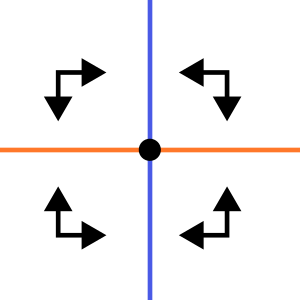
\includegraphics{Modellering/figuren/equi_stable.png} \\
Instabiel punt & Unstable point & Alle pijltjes wijzen van het evenwicht
weg. & 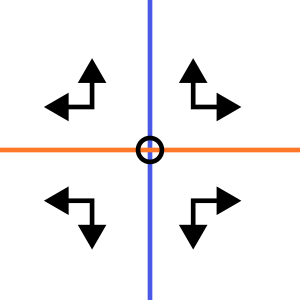
\includegraphics{Modellering/figuren/equi_unstable.png} \\
Zadelpunt & Saddle point & Sommige pijltjes wijzen naar het evenwicht
toe, en anderen ervan weg. &
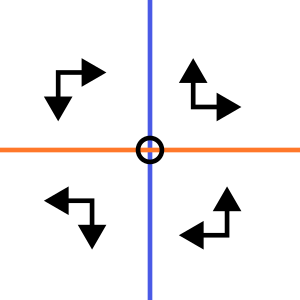
\includegraphics{Modellering/figuren/equi_saddle.png} \\
Stabiele spiraal & Stable spiral & Het vectorveld draait om het
evenwicht heen, maar uiteindelijk beweegt het systeem naar het evenwicht
toe. & 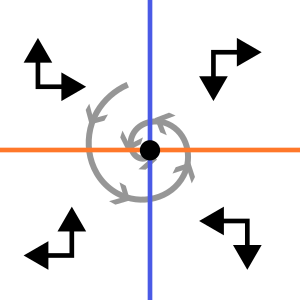
\includegraphics{Modellering/figuren/equi_spiral.png} \\
Instabiele spiraal & Unstable spiral & Het vectorveld draait om het
evenwicht heen, en het systeem beweegt weg van het evenwicht. &
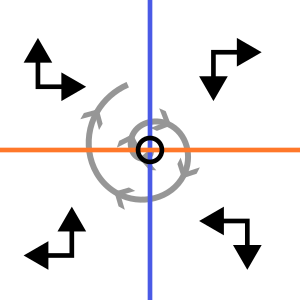
\includegraphics{Modellering/figuren/equi_spiral_unst.png} \\
\end{longtable}

\end{tcolorbox}

\hypertarget{opgaven-5}{%
\section{Opgaven}\label{opgaven-5}}

\begin{exercise}[Het ``werkelijke''
vectorveld]\protect\hypertarget{exr-vectorveld}{}\label{exr-vectorveld}

Het vectorveld hebben we tot nu toe versimpeld door slechts voor enkele
punten aan te geven of de variabelen langs de x- en y-as zullen afnemen
of toenemen. In werkelijkheid is dit vectorveld veel gedetailleerder:
het geeft voor elk punt in de ruimte de \emph{unieke richting} aan
waarin het systeem zich beweegt (zie onderstaande figuur).

\begin{figure}

{\centering 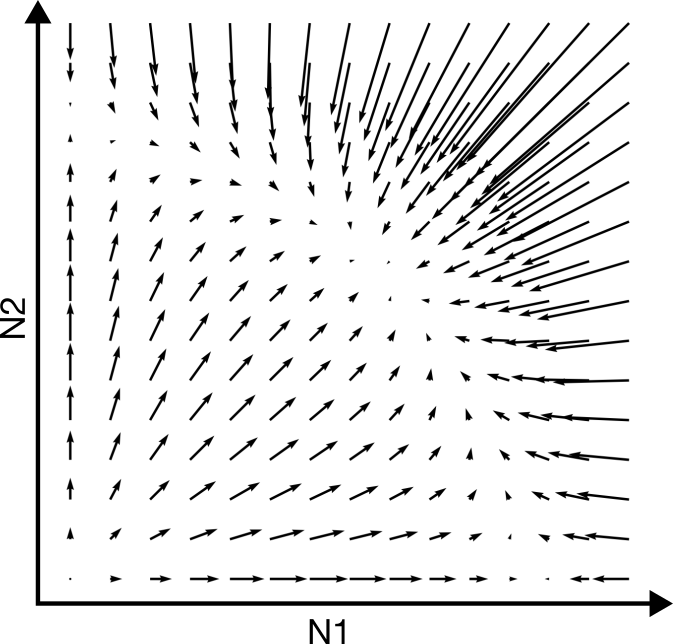
\includegraphics[width=0.5\textwidth,height=\textheight]{Modellering/figuren/vectorveld.png}

}

\end{figure}

Het bovenstaande vectorveld hoort bij het Lotka-Volterra competitie
model zoals besproken in dit hoofdstuk (let op: dit is weergegeven
\textbf{zonder} de nullclines).

\begin{enumerate}
\def\labelenumi{\alph{enumi}.}
\tightlist
\item
  Is in bovenstaande vectorveld de inter- of intraspecifieke competitie
  sterker? \emph{er is een evenwicht in het midden, dus intra is
  sterker}
\item
  Kan je in een ODE met dezelfde begincondities verschillende richtingen
  op gaan? Waarom wel/niet? \emph{nee dat kan niet, want voor elke
  waarde van X en Y krijg je een specifieke hoeveelheid groei van X en
  Y. Je gaat dus altijd dezelfde kant op. }
\item
  Leg met je antwoord op b uit waarom een trajectorie zichzelf nooit zal
  kunnen snijden. \emph{Hetzelfde als a. Je kan niet met dezelfde waarde
  meerdere kanten op gaan, wat bij snijden wel zo zou zijn!}
\item
  In werkelijkheid kan het weldegelijk zo zijn dat je een experiment
  onder dezelfde begincondities hebt gestart, en toch andere uitkomsten
  hebt. Geef twee verschillende redenen waarom dit in het experiment wel
  kan, en in je model niet. \emph{rede 1: er is geen ruis in het model,
  maar in werkelijkheid wel, rede 2 kunnen ze op veel manieren
  uitdrukken: er is geen hidden (derde of vierde) variabele / iets
  anders intefereert, etc.}
\item
  Als een trajectorie een nullcline snijdt, gaat dat altijd onder een
  hele specifieke hoek. Druk in woorden uit waarom dat is, en in welke
  hoek je door de nullclines kan gaan. \emph{op de nullcline is de
  richting van een van de variabelen 0, dus je kan er alleen precies
  horizontaal of precies verticaal doorheen gaan.}
\end{enumerate}

\end{exercise}

\begin{exercise}[Evenwichten en
trajectories]\protect\hypertarget{exr-evenwichtentraj}{}\label{exr-evenwichtentraj}

~

\begin{figure}

\begin{minipage}[t]{0.33\linewidth}

{\centering 

\raisebox{-\height}{

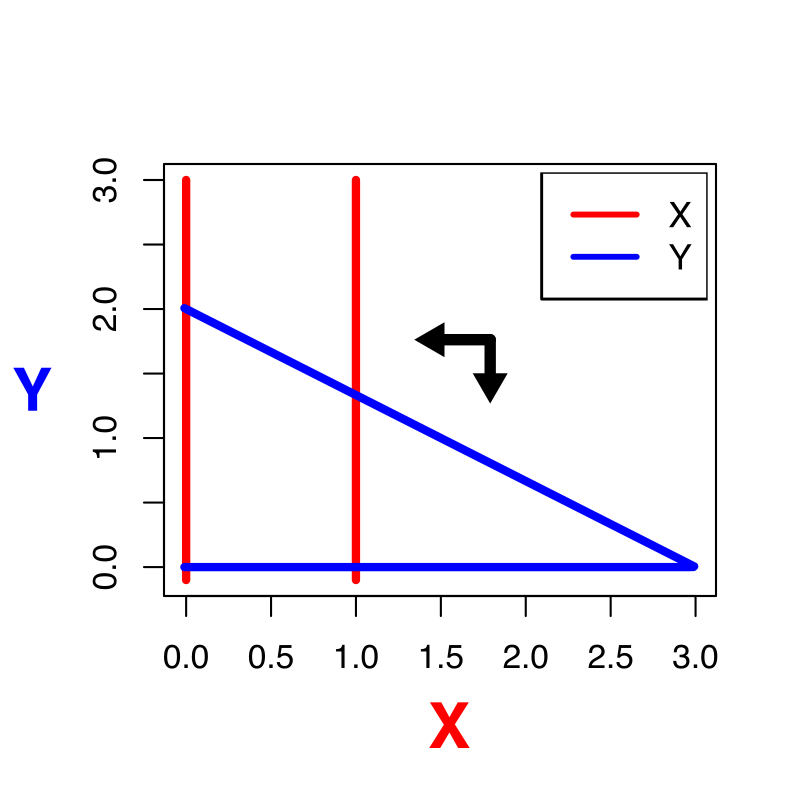
\includegraphics{Modellering/figuren/faseruimtevraag_1.png}

}

}

\subcaption{\label{fig-vraag_nullclines-1}\textbf{?(caption)}}
\end{minipage}%
%
\begin{minipage}[t]{0.33\linewidth}

{\centering 

\raisebox{-\height}{

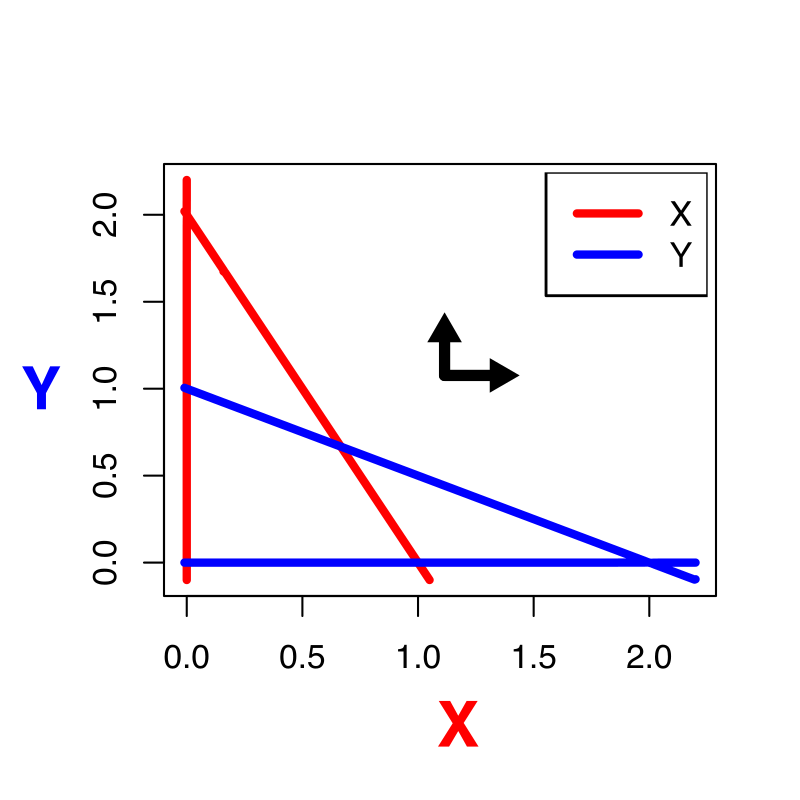
\includegraphics{Modellering/figuren/faseruimtevraag_2.png}

}

}

\subcaption{\label{fig-vraag_nullclines-2}\textbf{?(caption)}}
\end{minipage}%
%
\begin{minipage}[t]{0.33\linewidth}

{\centering 

\raisebox{-\height}{

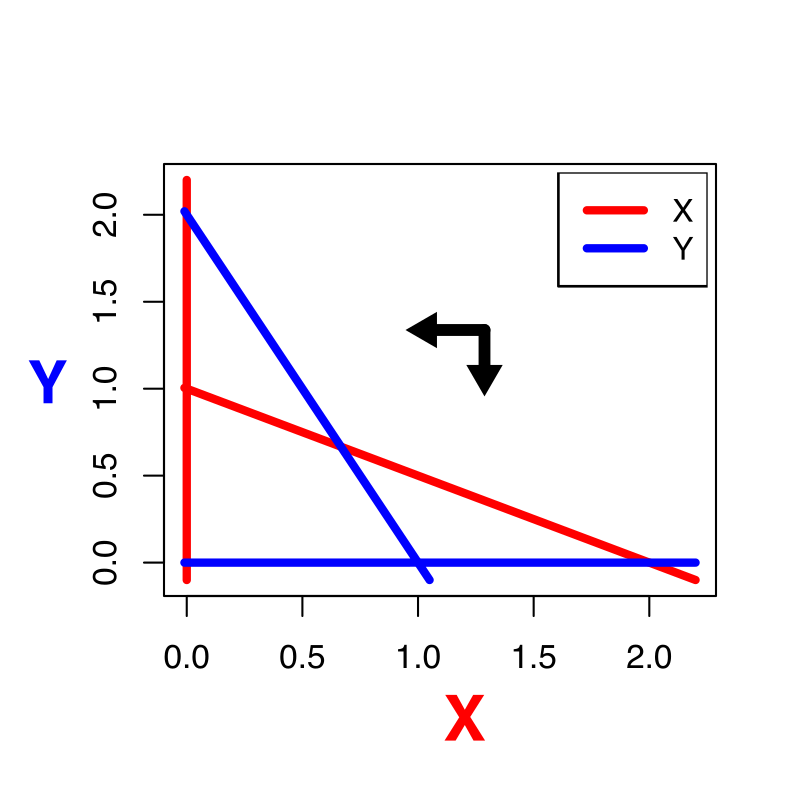
\includegraphics{Modellering/figuren/faseruimtevraag_3.png}

}

}

\subcaption{\label{fig-vraag_nullclines-3}\textbf{?(caption)}}
\end{minipage}%

\caption{\label{fig-competition_nullclines}Verschillende faseruimtes met
nullclines, waarbij slechts in 1 hoek het vectorveld is gegeven}

\end{figure}

In de bovenstaande faseruimtes zijn al nullclines getekend, en het
vectorveld is aangegeven voor 1 hoek.

\begin{enumerate}
\def\labelenumi{\alph{enumi}.}
\tightlist
\item
  Vul de rest van het vectorveld in en benoem de evenwichten (zie
  (\textbf{tip-typeevenwichten?}) voor de namen voor de verschillende
  typen evenwichten) \emph{de eerste is een beetje een instinker: lijkt
  op LV, maar is stabiel. midden is instabiel, rechts is zadelpunt.}
\item
  Stel we beginnen met X=0.1 en Y=0.2. Schets in elke faseruimte een
  geldige trajectorie \emph{schets 1: direct naar het evenwicht (mag wel
  krom maar je kan niet over nullclines heen! schets 2: naar oorsprong
  (0,0), schets 3: eerst nemen beide soorten toe, maar dan gaat het naar
  x,y = 0,0.2 }
\item
  Schets voor elke trajectory uit de vorige vraag een geldige oplossing
  (dat zijn dus twee ``grafiekjes door de tijd''). \emph{schets 1:
  asymptotisch naar evenwicht. schets 2: asymptotisch naar 0, schets 3:
  eerst nemen beide soorten toe, maar dan neemt x af en blijft y
  toenemen tot een evenwichtswaarde.}
\end{enumerate}

\end{exercise}

\begin{exercise}[Cheaters en
cooperators]\protect\hypertarget{exr-cheatandcoop}{}\label{exr-cheatandcoop}

In hoofdstuk Hoofdstuk~\ref{sec-ruimtelijk} heb je kennis gemaakt met
\emph{individual based modelling}, en heb je gezien hoe cooperators en
cheaters kunnen samenleven. Echter zagen we ook dat hoe meer we het
systeem mengde, hoe slechter dat ging. Sterker nog, onder goed gemengde
condities ging het eigenlijk nooit goed, omdat de cheaters teveel
toenamen en daarna het hele systeem uitstierf. Laten we kijken hoe dit
uitpakt in een ODE die vergelijkbare aannames doet. Bekijk het volgende
ODE model:

\begin{align*}
\mathchoice{\frac{\mathrm{d}C_1}
{\mathrm{d}t}}{\mathrm{d}C_1/\mathrm{d}t}
{\mathrm{d}C_1/\mathrm{d}t}
{\mathrm{d}C_1/\mathrm{d}t} &= b_1C_1^2(1-\frac{C_1+C_2}{K}) - dC_1\\
\mathchoice{\frac{\mathrm{d}C_2}
{\mathrm{d}t}}{\mathrm{d}C_2/\mathrm{d}t}
{\mathrm{d}C_2/\mathrm{d}t}
{\mathrm{d}C_2/\mathrm{d}t} &= b_2C_1C_2(1-\frac{C_1+C_2}{K}) - dC_2
\end{align*}

Anders dan in het individual-based model, waar we twee cooperators en
één cheater hadden, beschrijven we nu alleen een populatie van
cooperators en een populatie van cheaters. De parameters \(b_1\) en
\(b_2\) kunnen onderling verschillen, maar beide soorten hebben dezelfde
death rate \(d\).

\begin{enumerate}
\def\labelenumi{\alph{enumi}.}
\tightlist
\item
  Welk van de twee populaties is de cooperator, en welke de cheater?
  Waar zie je dit aan? \emph{C1 cooperator want de groeisnelheid is
  alleen van C1 afhankelijk. C2 is van C1 en C2 afhankelijk, en is dus
  de cheater.}
\item
  Waarom bevat de functionele response \((1-\frac{C_1+C_2}{K})\) zowel
  \(C_1\) als \(C_2\)? \emph{Dit genereert competitie tussen de twee
  soorten. We zijn geintresseerd in het samenleven van cooperator en
  cheater. Door ze een gedeelde carrying capacity te geven kunnen we
  onderzoeken wanneer ze kunnen samenleven.}
\item
  Als we een in de IBM een grid van 100x100 hadden, hoe groot zou \(K\)
  dan zijn? \emph{K is dan ongeveer 100x100 (min een beetje death), want
  het grid bepaalde in de IBM de maximale populatiegrootte.}
\end{enumerate}

Neem de volgende Grind code over, waar de cooperators iets sneller
groeien dan de cheaters:

\begin{Shaded}
\begin{Highlighting}[]
\FunctionTok{source}\NormalTok{(}\StringTok{"https://tbb.bio.uu.nl/rdb/grindR/grind.R"}\NormalTok{)}

\NormalTok{model }\OtherTok{\textless{}{-}} \ControlFlowTok{function}\NormalTok{(t, state, parms)\{}
  \FunctionTok{with}\NormalTok{(}\FunctionTok{as.list}\NormalTok{(}\FunctionTok{c}\NormalTok{(state,parms)),\{}
\NormalTok{    dC1 }\OtherTok{\textless{}{-}}\NormalTok{ b1}\SpecialCharTok{*}\NormalTok{C1}\SpecialCharTok{*}\NormalTok{C1}\SpecialCharTok{*}\NormalTok{(}\DecValTok{1}\SpecialCharTok{{-}}\NormalTok{C1}\SpecialCharTok{{-}}\NormalTok{C2) }\SpecialCharTok{{-}}\NormalTok{ d}\SpecialCharTok{*}\NormalTok{C1}
\NormalTok{    dC2 }\OtherTok{\textless{}{-}}\NormalTok{ b2}\SpecialCharTok{*}\NormalTok{C1}\SpecialCharTok{*}\NormalTok{C2}\SpecialCharTok{*}\NormalTok{(}\DecValTok{1}\SpecialCharTok{{-}}\NormalTok{C1}\SpecialCharTok{{-}}\NormalTok{C2) }\SpecialCharTok{{-}}\NormalTok{ d}\SpecialCharTok{*}\NormalTok{C2}
    \FunctionTok{return}\NormalTok{(}\FunctionTok{list}\NormalTok{(}\FunctionTok{c}\NormalTok{(dC1,dC2)))}
\NormalTok{  \})}
\NormalTok{\}  }

\NormalTok{colors[}\DecValTok{1}\NormalTok{] }\OtherTok{=} \StringTok{"orange"}
\NormalTok{colors[}\DecValTok{2}\NormalTok{] }\OtherTok{=} \StringTok{"blue"}

\NormalTok{p }\OtherTok{\textless{}{-}} \FunctionTok{c}\NormalTok{(}\AttributeTok{b1=}\FloatTok{2.0}\NormalTok{,}\AttributeTok{b2=}\DecValTok{1}\NormalTok{,}\AttributeTok{d=}\FloatTok{0.1}\NormalTok{)}
\NormalTok{s }\OtherTok{\textless{}{-}} \FunctionTok{c}\NormalTok{(}\AttributeTok{C1=}\FloatTok{0.2}\NormalTok{,}\AttributeTok{C2=}\FloatTok{0.1}\NormalTok{)}
\FunctionTok{plane}\NormalTok{(}\AttributeTok{vector=}\NormalTok{T,}\AttributeTok{grid=}\DecValTok{7}\NormalTok{)}
\end{Highlighting}
\end{Shaded}

\begin{enumerate}
\def\labelenumi{\alph{enumi}.}
\setcounter{enumi}{3}
\tightlist
\item
  Bestudeer de faseruimte en het vectorveld. Is het evenwicht met alleen
  cooperators en géén cheaters stabiel, of instabiel? Controlleer je
  antwoord met \texttt{newton(c(C1=1,C2=0),plot=T)} \emph{stabiel}
\item
  Voorspel wie er overleeft wanneer je begint met veel van beide
  soorten. \emph{alleen cooperators}
\item
  Voorspel wie er overleeft wanneer je begint met weinig van beide
  soorten. \emph{niemand}
\end{enumerate}

We gaan nu aannemen dat de cheaters sneller groeien dan de cooperators
(draai hiervoor de waarde van \(b_1\) en \(b_2\) om).

\begin{enumerate}
\def\labelenumi{\alph{enumi}.}
\setcounter{enumi}{6}
\tightlist
\item
  Bestudeer opnieuw de faseruimte en het vectorveld. Is het evenwicht
  met alleen cooperators stabiel of instabiel? \emph{instabiel}
\item
  Voorspel opnieuw wie er overleeft, en hoe dat afhangt van de
  begin-dichtheden. Leg in biologische termen uit wat er gebeurt.
  \emph{maakt niet uit hoe je begint, alles gaat altijd dood}
\item
  Bestudeer andere waarden van \(b_1\) en \(b_2\). Bij welke parameters
  kunnen zowel \(C_1\) als \(C_2\) blijven leven? Vind je de gevonden
  voorwaarde biologisch relevant? \emph{als b1 en b2 gelijk zijn. Niet
  heel relevant dus.}
\end{enumerate}

In de simulatie hieronder is de birth rate van cooperators iets lager
gemaakt dan die van de cheaters.

\begin{enumerate}
\def\labelenumi{\alph{enumi}.}
\setcounter{enumi}{9}
\tightlist
\item
  Hoe kan het dat het individual-based model coexistentie van de soorten
  laat zien, terwijl dit in de ODE niet kan? \emph{het samenleven werkt
  alleen als je niet mengt. met mengen sterft alles uit, dus kennelijk
  is de ruimtelijke structuur belangrijk. dit kan je ook wel zien, want
  lokaal (in een klein stukje van de simulatie) is er WEL steeds sprake
  van uitsterven. maar dan is het niet onmiddelelijk einde verhaal!}
\end{enumerate}

\end{exercise}

\begin{exercise}[Parameter
fitting\}]\protect\hypertarget{exr-parfitting}{}\label{exr-parfitting}

\begin{figure}

{\centering 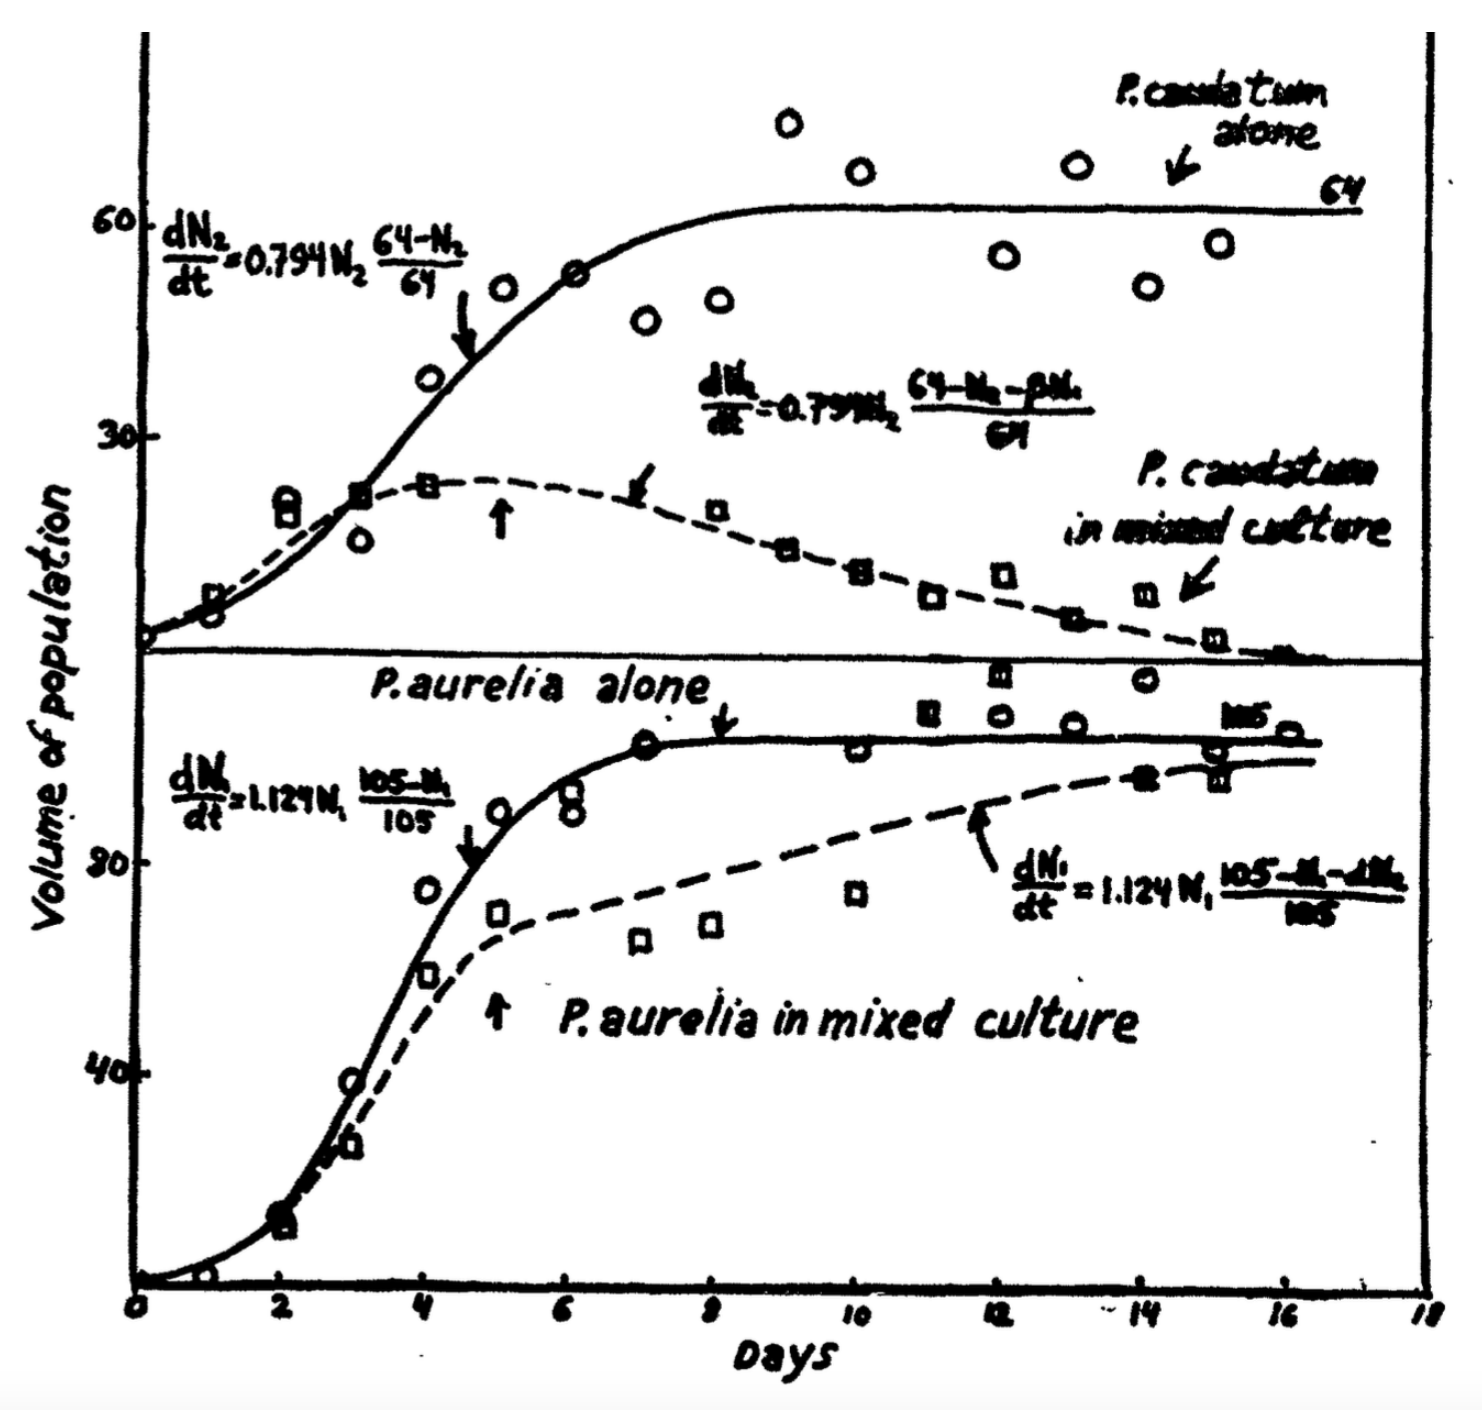
\includegraphics[width=0.8\textwidth,height=\textheight]{Modellering/figuren/gausfit.png}

}

\caption{Figuur 1 uit Gause (1934)}

\end{figure}

In klassieke experimenten groeide Gause (1934) twee soorten
\emph{Paramecium}, zowel in isolatie als samen. De doorgetrokken lijnen
in de figuur hierboven suggereren dat de groeicurve van \emph{P.
aurelia} en \emph{P. caudatum} in isolatie redelijk goed beschreven
worden door een logistische groeivergelijking. In Gause's eigen
handschrift zijn de geschatte parameterwaarden te lezen (\(r\) = 0,794
per dag met \(K\) = 64 voor \emph{P. caudatum} en \(r = 1,129\) per dag
met \(K = 105\) voor \emph{P. aurelia}). We gaan deze parameter-waarden
bestuderen met Grind. Neem het volgende script over:

\begin{Shaded}
\begin{Highlighting}[]
\FunctionTok{source}\NormalTok{(}\StringTok{"https://tbb.bio.uu.nl/rdb/grindR/grind.R"}\NormalTok{)}

\NormalTok{model }\OtherTok{\textless{}{-}} \ControlFlowTok{function}\NormalTok{(t, state, parms) \{}
  \FunctionTok{with}\NormalTok{(}\FunctionTok{as.list}\NormalTok{(}\FunctionTok{c}\NormalTok{(state,parms)), \{}
\NormalTok{    dtN }\OtherTok{\textless{}{-}}\NormalTok{ r}\SpecialCharTok{*}\NormalTok{N}\SpecialCharTok{*}\NormalTok{(}\DecValTok{1} \SpecialCharTok{{-}}\NormalTok{ N}\SpecialCharTok{/}\NormalTok{K)}
    \FunctionTok{return}\NormalTok{(}\FunctionTok{list}\NormalTok{(}\FunctionTok{c}\NormalTok{(dtN)))  }
\NormalTok{  \}) }
\NormalTok{\} }

\NormalTok{p }\OtherTok{\textless{}{-}} \FunctionTok{c}\NormalTok{(}\AttributeTok{r=}\DecValTok{1}\NormalTok{,}\AttributeTok{K=}\DecValTok{100}\NormalTok{)    }\CommentTok{\# Een ruwe gok van de parameters}
\NormalTok{s }\OtherTok{\textless{}{-}} \FunctionTok{c}\NormalTok{(}\AttributeTok{N=}\DecValTok{2}\NormalTok{)}
\FunctionTok{run}\NormalTok{(}\DecValTok{18}\NormalTok{)              }\CommentTok{\# Run het model 18 tijdstappen}
\end{Highlighting}
\end{Shaded}

\begin{enumerate}
\def\labelenumi{\alph{enumi}.}
\tightlist
\item
  Waarom denk je dat we het model voor slechts 18 tijdstappen
  doorrekenen? \emph{het experiment is 18 dagen}
\item
  De ruwe data voor de soorten in isolatie (dus de rondjes in de figuur
  hierboven) staan op de website. Deze kan je zelf plotten, maar Grind
  heeft ook hier een ingebouwde functie voor (zie onderstaande code):
\end{enumerate}

\begin{Shaded}
\begin{Highlighting}[]
\NormalTok{  caudatum }\OtherTok{\textless{}{-}} \FunctionTok{read.table}\NormalTok{(}\StringTok{"https://tbb.bio.uu.nl/bvd/bms/caudatum.txt"}\NormalTok{, }\AttributeTok{header=}\ConstantTok{TRUE}\NormalTok{)}
  \FunctionTok{timePlot}\NormalTok{(caudatum,}\AttributeTok{draw=}\NormalTok{points)}
\NormalTok{  p }\OtherTok{\textless{}{-}} \FunctionTok{c}\NormalTok{(}\AttributeTok{r=}\DecValTok{2}\NormalTok{,}\AttributeTok{K=}\DecValTok{50}\NormalTok{)   }
\NormalTok{  s }\OtherTok{\textless{}{-}} \FunctionTok{c}\NormalTok{(}\AttributeTok{N=}\DecValTok{3}\NormalTok{)}
  \FunctionTok{run}\NormalTok{(}\DecValTok{18}\NormalTok{,}\AttributeTok{add=}\NormalTok{T)}
\end{Highlighting}
\end{Shaded}

In de laatste regel code wordt het Grind-model over de data heen geplot.

\begin{enumerate}
\def\labelenumi{\alph{enumi}.}
\setcounter{enumi}{2}
\tightlist
\item
  Probeer door \emph{trial-and-error} een betere fit te krijgen aan de
  data (let op: je kunt zowel de parameters \(r\) en \(K\), als de
  initiele conditie van \(N\) aanpassen).
\item
  Tot hoeveel decimalen heb je \(r\), \(K\), en \(N\) geschat? Vertrouw
  je de uitkomst, en wellicht belangrijker, kun je dit vertrouwen
  objectief onderbouwen? \emph{eigenlijk kan je met 0 decimalen al wel
  een aardige fit krijgen, maar je weet dan niet per se hoe goed die is}
\end{enumerate}

\emph{Trial-and-error} is niet reproduceerbaar voor andere
wetenschappers, en is bovendien een enorm gepruts als je nog meer
parameters hebt! Grind kan daarom ook parameters-fitting doen:
automatisch veel mogelijke parameters uitproberen om zo tot een goede
(hopelijk de beste) ``fit'' te komen:

\begin{Shaded}
\begin{Highlighting}[]
\NormalTok{    caudatum }\OtherTok{\textless{}{-}} \FunctionTok{read.table}\NormalTok{(}\StringTok{"https://tbb.bio.uu.nl/bvd/bms/caudatum.txt"}\NormalTok{, }\AttributeTok{header=}\ConstantTok{TRUE}\NormalTok{)}
    \FunctionTok{timePlot}\NormalTok{(caudatum,}\AttributeTok{draw=}\NormalTok{points)}
\NormalTok{    p }\OtherTok{\textless{}{-}} \FunctionTok{c}\NormalTok{(}\AttributeTok{r=}\DecValTok{1}\NormalTok{,}\AttributeTok{K=}\DecValTok{10}\NormalTok{)   }
\NormalTok{    s }\OtherTok{\textless{}{-}} \FunctionTok{c}\NormalTok{(}\AttributeTok{N=}\DecValTok{2}\NormalTok{)}
    \FunctionTok{run}\NormalTok{(}\DecValTok{18}\NormalTok{,}\AttributeTok{add=}\NormalTok{T)}
\NormalTok{    free }\OtherTok{\textless{}{-}} \FunctionTok{c}\NormalTok{(}\StringTok{"r"}\NormalTok{,}\StringTok{"K"}\NormalTok{,}\StringTok{"N"}\NormalTok{)}
\NormalTok{    fC }\OtherTok{\textless{}{-}} \FunctionTok{fit}\NormalTok{(caudatum,}\AttributeTok{free=}\NormalTok{free,}\AttributeTok{main=}\StringTok{"Caudatum"}\NormalTok{,}\AttributeTok{legend=}\ConstantTok{FALSE}\NormalTok{)}
\end{Highlighting}
\end{Shaded}

\begin{verbatim}
e. Wat denk je dat er in deze code wordt bedoeld met 'free'? *dit zijn de vrije parameters, als je bijv. N weghaald kan deze niet varieren tijdens het fitten*
f. Voer de bovenstaande code uit voor zowel de gegeven waarden ($r=1$, $K=10$, $N=2$), als de waarden die je met \textit{trial-and-error} gevonden hebt. Is het eind-resultaat (de parameter-schattingen) vergelijkbaar? *nagenoeg hetzelfde, kleine verschillen, let op voor verdiepend antwoordenmodel: hoeft niet zo te zijn. soms zijn er meerdere fits mogelijk afh van de initial conditie.*
\end{verbatim}

Om de betrouwbaarheid van de fit te bestuderen, kunnen we de functie
`summary' in R gebruiken om de fit samen te vatten:

\begin{Shaded}
\begin{Highlighting}[]
\NormalTok{fC }\OtherTok{\textless{}{-}} \FunctionTok{fit}\NormalTok{(caudatum,}\AttributeTok{free=}\NormalTok{free,}\AttributeTok{main=}\StringTok{"Caudatum"}\NormalTok{,}\AttributeTok{legend=}\ConstantTok{FALSE}\NormalTok{)}
\FunctionTok{summary}\NormalTok{(fC)}
\end{Highlighting}
\end{Shaded}

\begin{verbatim}
   Estimate Std. Error t value Pr(>|t|)    
r   0.7623     0.2221   3.433  0.00496 ** 
K  60.9539     3.2774  18.598 3.25e-10 ***
N   3.7722     2.8796   1.310  0.21473 
--
Signif. codes:  0 ‘***’ 0.001 ‘**’ 0.01 ‘*’ 0.05 ‘.’ 0.1 ‘ ’ 1

Residual standard error: 8.195 on 12 degrees of freedom

Parameter correlation:
        r       K       N
r  1.0000 -0.4381 -0.9272
K -0.4381  1.0000  0.3023
N -0.9272  0.3023  1.0000
\end{verbatim}

Deze samenvatting geeft naast de parameter-waarden ook een boel andere
statistiek (standaard error, P-waarden, correlaties). Wat deze termen
betekenen, en hoe je ze moet interpreteren, leer je bij het onderdeel
statistiek.

\end{exercise}

\hypertarget{terminologie-7}{%
\section{Terminologie}\label{terminologie-7}}

\begin{longtable}[]{@{}
  >{\raggedright\arraybackslash}p{(\columnwidth - 4\tabcolsep) * \real{0.2500}}
  >{\raggedright\arraybackslash}p{(\columnwidth - 4\tabcolsep) * \real{0.2778}}
  >{\raggedright\arraybackslash}p{(\columnwidth - 4\tabcolsep) * \real{0.4722}}@{}}
\toprule\noalign{}
\begin{minipage}[b]{\linewidth}\raggedright
Nederlands
\end{minipage} & \begin{minipage}[b]{\linewidth}\raggedright
Engels
\end{minipage} & \begin{minipage}[b]{\linewidth}\raggedright
Beschrijving
\end{minipage} \\
\midrule\noalign{}
\endhead
\bottomrule\noalign{}
\endlastfoot
Intraspecifieke competitie & Intraspecific competition & Competitie
binnen een soort (tussen soortgenoten) \\
Interspecifieke competitie & Interspecific competition & Competitie
tussen soort \\
Coexistentie & Coexistence & De samenleving van twee of meerdere
soorten. \\
Competitieve exclusie & Competitive exclusion & Twee soorten die niet
duurzaam kunnen samenleven; de ene zal de andere verdringen. \\
Parameter fitting & Parameter fitting & Het zoeken naar de parameters
waarmee een model (bijvoorbeeld een ODE) overeenkomt met de data. Let
op: er is niet altijd één set parameters die de data goed kan
beschrijven! \\
\end{longtable}

\hypertarget{evolutie-en-biodiversiteit}{%
\chapter{Evolutie en biodiversiteit}\label{evolutie-en-biodiversiteit}}

Tot nu toe heb je veel geleerd over essentiële ecologische processen
zoals groei, interacties tussen individuen, concurrentie en
co-existentie. De individuen waar het in deze modellen om gaat, kunnen
niet alleen konijnen en vossen zijn, maar ook bacteriën, immuun-cellen
of tumorcellen. Met deze modellen kunnen we dus niet alleen fundamenteel
onderzoek uitvoeren, maar ook een belangrijke bijdrage leveren aan het
verbeteren van de menselijke gezondheid. Waarom is antimicrobiële
resistentie zo sterk toegenomen? Waarom reageert de ene tumor beter op
behandeling dan de andere? Waarom beginnen nieuwe virusen (zoals
Covid-19) zeer schadelijk, maar worden ze uiteindelijk vaak milder? Om
deze vragen te beantwoorden gaan we in dit hoofdstuk leren hoe 2D ODEs
zich vertalen naar evolutionaire vraagstukken.

Naast het ontstaan van diversiteit, kunnen we ook vragen stellen over
het behoud van biodiversiteit. Het behoud van biodiversiteit is
natuurlijk erg belangrijk: niet alleen is de natuur erg mooi, maar ook
zijn we als maatschappij zeer afhankelijk van gezonde en veerkrachtige
ecosystemen. Zo beschermen deze ons tegen overstromingen en zandstormen,
en bevorderd diversiteit het de nutrientenkringloop (en dus
vruchtbaarheid) in de landbouw. Maar welke factoren spelen hier
eigenlijk een belangrijke rol? Is een ecosysteem robust als er veel
cooperatie is, of juist als er veel competitie is? Om deze vragen te
kunnen beantwoorden moeten we naar systemen van meer dan twee soorten
gaan kijken.

\begin{figure}

{\centering \includegraphics[width=0.7\textwidth,height=\textheight]{Modellering/figuren/evolution_intro_AI.png}

}

\end{figure}

\hypertarget{leerdoelen-8}{%
\section{Leerdoelen}\label{leerdoelen-8}}

De leerdoelen van dit hoofdstuk zijn:

\begin{itemize}
\tightlist
\item
  Begrijpen hoe je met ODEs evolutionaire vragen kan stellen
\item
  Kunnen omschrijven hoe niche-overlap vertaalt in specifieke
  competitie-parameters
\item
  Omschrijven hoe een ecosysteem zich vertaalt in vele ODEs, en hoe
  interactie-matrices gebruikt kunnen worden om deze te modelleren
\item
  Aan een faseruimte kunnen herkennen of er sprake is van \emph{founder
  control}
\item
  Begrijpen hoe \emph{founder control} in ruimtelijke modellen
  overwonnen kan worden
\end{itemize}

\hypertarget{invasie-bestuderen-met-odes}{%
\section{Invasie bestuderen met
ODEs}\label{invasie-bestuderen-met-odes}}

Laten we beginnen met het intussen welbekende model van logistisch groei
met dichtheidsafhankelijke geboorte:

\begin{align*}
\mathchoice{\frac{\mathrm{d}N}
{\mathrm{d}t}}{\mathrm{d}N/\mathrm{d}t}
{\mathrm{d}N/\mathrm{d}t}
{\mathrm{d}N/\mathrm{d}t} &= bN(1-\frac{N}{K}) - dN
\end{align*}

Waarbij \(b\) de maximale birth rate is, \(d\) de vaste death rate, en
\(K\) de schalingsfactor voor dichtheidsafhankelijke afname van
reproductie. Hoewel \(K\) vooral bepaald wordt door eigenschappen in de
omgeving (de hoeveelheid eten bijvoorbeeld), kan je misschien wel jezelf
wel voorstellen dat \(b\) en \(d\) eigenschappen die uniek zijn voor
elke soort, of misschien zelfs voor elk individu binnen deze soort. In
een evolutionaire context kunnen we deze parameters ``evolueerbaar''
noemen: er kunnen op elk moment mutanten ontstaan met een andere
birth/death rate. Maar zullen deze mutanten zich dan verspreiden?
Hiervoor kunnen we ons 1D ODE model weer uitbreiden naar een 2D ODE
systeem:

\begin{align*}
\mathchoice{\frac{\mathrm{d}N}
{\mathrm{d}t}}{\mathrm{d}N/\mathrm{d}t}
{\mathrm{d}N/\mathrm{d}t}
{\mathrm{d}N/\mathrm{d}t} &= b_NN(1-\frac{N+M}{K}) - d_NN\\
\mathchoice{\frac{\mathrm{d}M}
{\mathrm{d}t}}{\mathrm{d}M/\mathrm{d}t}
{\mathrm{d}M/\mathrm{d}t}
{\mathrm{d}M/\mathrm{d}t} &= b_MM(1-\frac{N+M}{K}) - d_MM
\end{align*}

Hier is \(N\) de oorspronkelijke soort (het zogeheten wildtype), en is
\(M\) de mutant met andere birth en/of death rates. Laten we bestuderen
wat er gebeurt als er een mutant ontstaat met een verlaagde death rate,
door de faseruimte te bestuderen. Hiervoor kunnen we de nullclines
bepalen door beide vergelijkinen gelijk te stellen aan \(0\), of we
plotten de nullclines met Grind (Figuur~\ref{fig-wildtypeandmutant})

\begin{Shaded}
\begin{Highlighting}[]
\FunctionTok{source}\NormalTok{(}\StringTok{"https://tbb.bio.uu.nl/rdb/grindR/grind.R"}\NormalTok{)}
\end{Highlighting}
\end{Shaded}

\begin{verbatim}
Warning: package 'deSolve' was built under R version 4.4.2
\end{verbatim}

\begin{verbatim}
Warning: package 'FME' was built under R version 4.4.2
\end{verbatim}

\begin{Shaded}
\begin{Highlighting}[]
\NormalTok{model }\OtherTok{\textless{}{-}} \ControlFlowTok{function}\NormalTok{(t, state, parms)\{}
  \FunctionTok{with}\NormalTok{(}\FunctionTok{as.list}\NormalTok{(}\FunctionTok{c}\NormalTok{(state,parms)),\{}
\NormalTok{    dN }\OtherTok{\textless{}{-}}\NormalTok{ bn}\SpecialCharTok{*}\NormalTok{N}\SpecialCharTok{*}\NormalTok{(}\DecValTok{1}\SpecialCharTok{{-}}\NormalTok{(N}\SpecialCharTok{+}\NormalTok{M)}\SpecialCharTok{/}\NormalTok{K) }\SpecialCharTok{{-}}\NormalTok{ dn}\SpecialCharTok{*}\NormalTok{N}
\NormalTok{    dM }\OtherTok{\textless{}{-}}\NormalTok{ bm}\SpecialCharTok{*}\NormalTok{M}\SpecialCharTok{*}\NormalTok{(}\DecValTok{1}\SpecialCharTok{{-}}\NormalTok{(N}\SpecialCharTok{+}\NormalTok{M)}\SpecialCharTok{/}\NormalTok{K) }\SpecialCharTok{{-}}\NormalTok{ dm}\SpecialCharTok{*}\NormalTok{M}
    \FunctionTok{return}\NormalTok{(}\FunctionTok{list}\NormalTok{(}\FunctionTok{c}\NormalTok{(dN,dM)))}
\NormalTok{  \})}
\NormalTok{\}  }

\NormalTok{colors[}\DecValTok{1}\NormalTok{] }\OtherTok{=} \StringTok{"orange"}
\NormalTok{colors[}\DecValTok{2}\NormalTok{] }\OtherTok{=} \StringTok{"blue"}

\NormalTok{p }\OtherTok{\textless{}{-}} \FunctionTok{c}\NormalTok{(}\AttributeTok{bn=}\DecValTok{1}\NormalTok{,}\AttributeTok{dn=}\FloatTok{0.2}\NormalTok{,}\AttributeTok{K=}\DecValTok{1}\NormalTok{, }\AttributeTok{dm=}\FloatTok{0.01}\NormalTok{, }\AttributeTok{bm=}\DecValTok{1}\NormalTok{)}
\NormalTok{s }\OtherTok{\textless{}{-}} \FunctionTok{c}\NormalTok{(}\AttributeTok{N=}\FloatTok{0.8}\NormalTok{,}\AttributeTok{M=}\FloatTok{0.0001}\NormalTok{)}
\FunctionTok{par}\NormalTok{(}\AttributeTok{mfrow=}\FunctionTok{c}\NormalTok{(}\DecValTok{1}\NormalTok{,}\DecValTok{2}\NormalTok{))}
\FunctionTok{plane}\NormalTok{(}\AttributeTok{vector=}\NormalTok{T,}\AttributeTok{grid=}\DecValTok{6}\NormalTok{,}\AttributeTok{ymax=}\FloatTok{1.1}\NormalTok{,}\AttributeTok{xmax=}\FloatTok{1.1}\NormalTok{)}

\FunctionTok{run}\NormalTok{(}\AttributeTok{tmax=}\DecValTok{100}\NormalTok{,}\AttributeTok{traject=}\NormalTok{F)}
\end{Highlighting}
\end{Shaded}

\begin{figure}[H]

{\centering 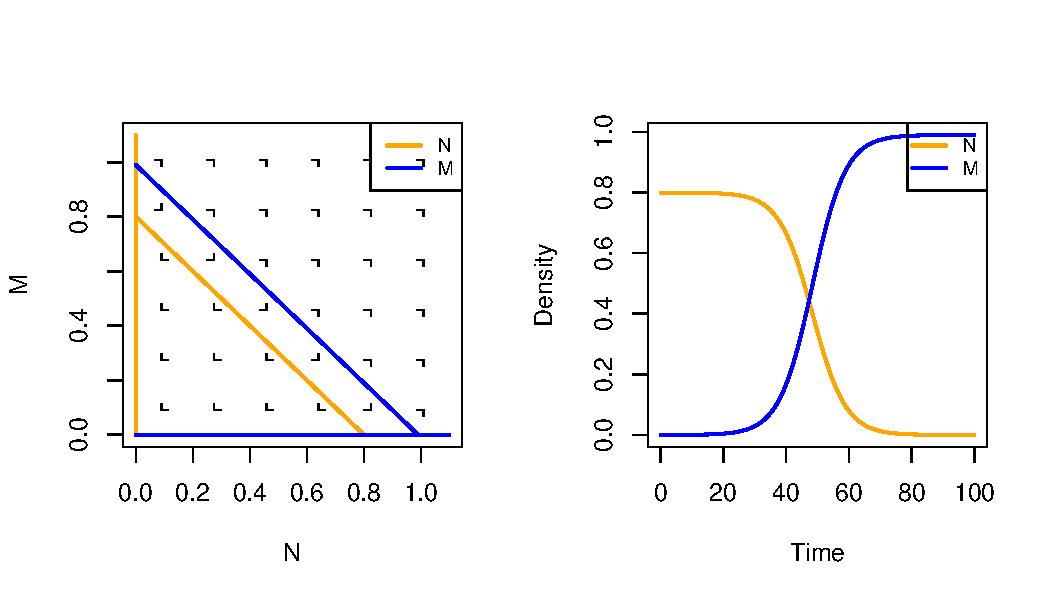
\includegraphics{Modellering/ecoevo_evolutiediversiteit_files/figure-pdf/fig-wildtypeandmutant-1.pdf}

}

\caption{\label{fig-wildtypeandmutant}CAPTION TODO}

\end{figure}

Het scenario hierboven kunnen we zien als een
\textbf{invasie-experiment}. Als een mutant (of een invasieve soort)
zich bevind in een gevestigde populatie, zal deze dan verspreiden? In
dit geval is het antwoord heel simpel: de soort met een lagere death
rate zal zich verspreiden, en de gevestigde soort volledig verdringen.

\hypertarget{niche-ruimte-en-diversiteit}{%
\section{Niche ruimte en
diversiteit}\label{niche-ruimte-en-diversiteit}}

In 1859 schreef Charles Darwin het boek \emph{``the origin of
species''}, waarin hij voor het eerst het proces van evolutie door
natuurlijke selectie omschreef. Een belangrijke observatie was dat de
verschillende vinken op de Galápagos eilanden hele verschillende snavels
hadden:

\begin{figure}

{\centering 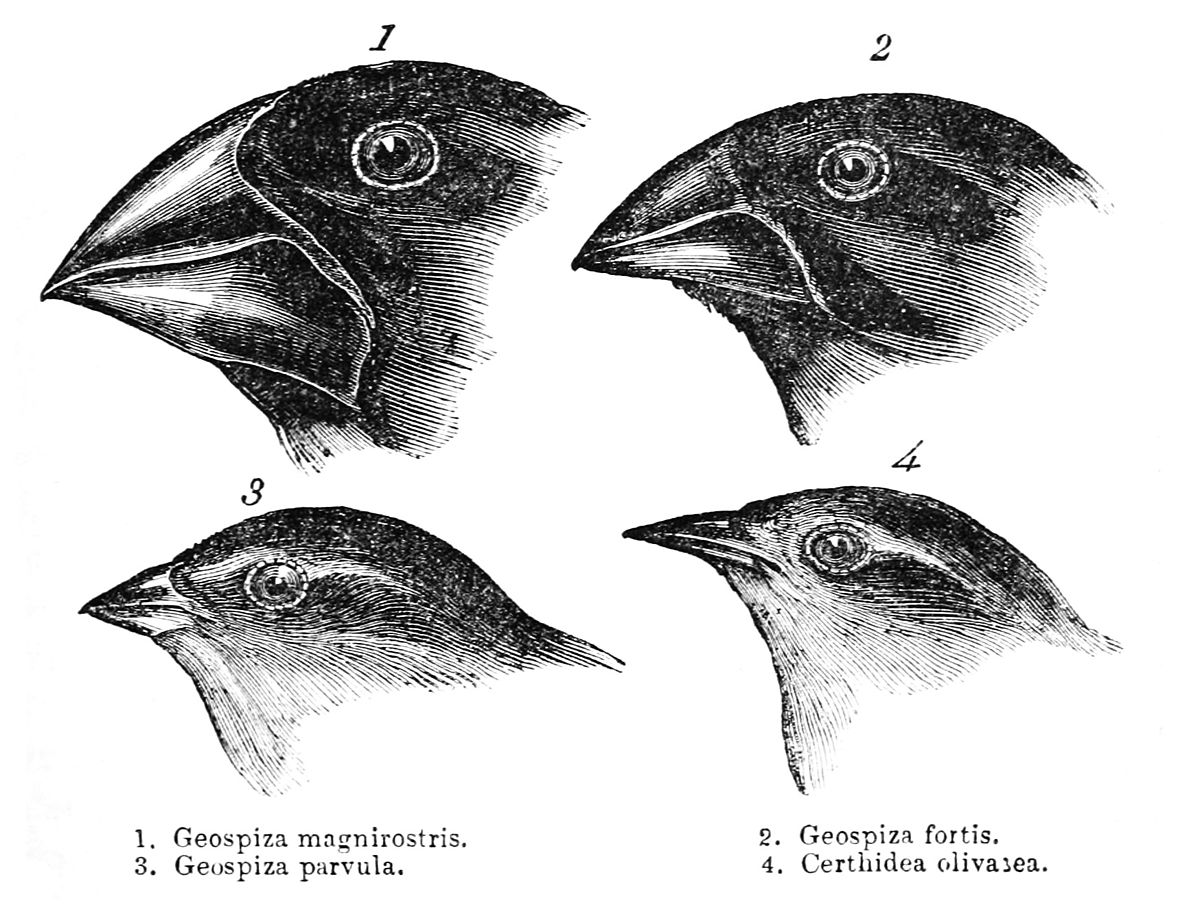
\includegraphics[width=0.7\textwidth,height=\textheight]{Modellering/figuren/darwin_finches.png}

}

\end{figure}

De snavels van deze vinken geven direct inzicht in de competitie om
voedsel: in een kleine snavel passen geen walnoten, maar met een grote
snavel kun je erg moeilijk kleine zaadjes oppikken. Deze verschillende
adaptaties in vinken vertalen zich direct naar niches zoals we die al
kort in hoofdstuk Hoofdstuk~\ref{sec-dichtheid} hebben besproken. We
kunnen ons bijvoorbeeld voorstellen dat twee vogels voorkeuren hebben
voor zaadjes met verschillende groottes. Dit zouden we als een
normaalverdeling kunnen weergeven (Figuur~\ref{fig-nicheoverlaps-1}),
die voorstellen welke zaadjes de verschillende vogelsoorten eten.

\begin{figure}

\begin{minipage}[t]{0.50\linewidth}

{\centering 

\raisebox{-\height}{

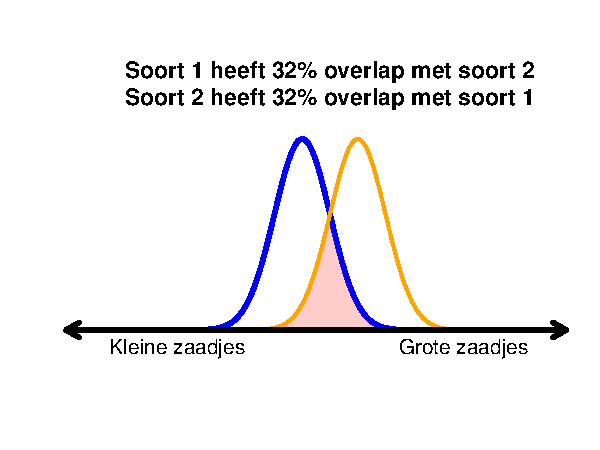
\includegraphics{Modellering/ecoevo_evolutiediversiteit_files/figure-pdf/fig-nicheoverlaps-1.pdf}

}

}

\subcaption{\label{fig-nicheoverlaps-1}Niche-overlap weergegeven als
normaalverdelingen}
\end{minipage}%
%
\begin{minipage}[t]{0.50\linewidth}

{\centering 

\raisebox{-\height}{

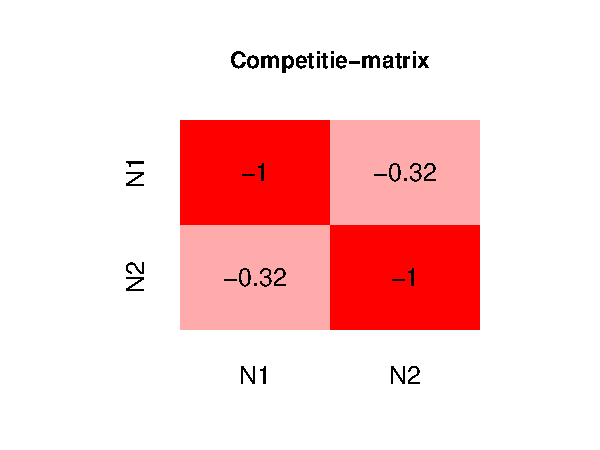
\includegraphics{Modellering/ecoevo_evolutiediversiteit_files/figure-pdf/fig-nicheoverlaps-2.pdf}

}

}

\subcaption{\label{fig-nicheoverlaps-2}Niche-overlap weergegeven als een
interactiematrix}
\end{minipage}%

\caption{\label{fig-nicheoverlaps}Niche-overlap voor twee vogelsoorten
met een andere voorkeur voor de grootte van zaadjes, maar met dezelfde
spreiding}

\end{figure}

Zoals je ziet overlappen de verdelingen uit
Figuur~\ref{fig-nicheoverlaps-1} deels. Dit vertaalt zich direct in
interspecifieke competitie: hoe meer de verdelingen overlappen, hoe meer
zaadjes door beide soorten gegeten worden, hoe meer competitie tussen de
soorten. Op dezelfde manier kunnen we definiëren dat de
\textbf{intra}specifieke competitie maximaal is: een soort ``overlapt''
altijd 100\% met zichzelf. Als we teruggaan naar het competitiemodel uit
het vorige hoofdstuk (zie Vergelijking~\ref{eq-soorten}), kunnen we deze
niche-overlap vertalen in specifieke waarden voor \(c_{11}\),
\(c_{12}\), \(c_{22}\), en \(c_{21}\). De soorten hebben volledige
overlap met zichzelf (\(c_{11}=c_{22}=1\)), en 32\% overlap met de ander
(\(c_{12}=c_{21}=0.32\)). Deze informatie kunnen we ook weergeven in een
zogeheten interactie-matrix (Figuur~\ref{fig-nicheoverlaps-2}). De
negatieve getallen in deze matrix betekenen dat de dichtheden van de
soorten alleen negatieve effecten op hun groei hebben. Daarom wordt een
dergelijke matrix ook wel een competitie-matrix kunnen noemen.

Deze niche-ruimtes zijn natuurlijk makkelijk te vertalen naar meerdere
soorten (Figuur~\ref{fig-nicheoverlaps2-1}), wat ook resulteert in een
grotere matrix (Figuur~\ref{fig-nicheoverlaps2-2}).

\begin{Shaded}
\begin{Highlighting}[]
\CommentTok{\# Meer soorten}

\CommentTok{\# Define the range for the x{-}axis}
\NormalTok{  x\_range }\OtherTok{\textless{}{-}} \FunctionTok{seq}\NormalTok{(}\SpecialCharTok{{-}}\DecValTok{5}\NormalTok{, }\DecValTok{5}\NormalTok{, }\AttributeTok{length.out =} \DecValTok{1000}\NormalTok{)}
  
  \CommentTok{\# Calculate the densities}
\NormalTok{  density1 }\OtherTok{\textless{}{-}} \FunctionTok{dnorm}\NormalTok{(x\_range, }\AttributeTok{mean =} \DecValTok{1}\NormalTok{, }\AttributeTok{sd =} \FloatTok{0.5}\NormalTok{)}
\NormalTok{  density2 }\OtherTok{\textless{}{-}} \FunctionTok{dnorm}\NormalTok{(x\_range, }\AttributeTok{mean =} \DecValTok{2}\NormalTok{, }\AttributeTok{sd =} \DecValTok{1}\NormalTok{)}
\NormalTok{  density3 }\OtherTok{\textless{}{-}} \FunctionTok{dnorm}\NormalTok{(x\_range, }\AttributeTok{mean =} \SpecialCharTok{{-}}\DecValTok{2}\NormalTok{, }\AttributeTok{sd =} \FloatTok{0.5}\NormalTok{)}
\NormalTok{  density4 }\OtherTok{\textless{}{-}} \FunctionTok{dnorm}\NormalTok{(x\_range, }\AttributeTok{mean =} \SpecialCharTok{{-}}\FloatTok{0.5}\NormalTok{, }\AttributeTok{sd =} \FloatTok{0.2}\NormalTok{)}
  
  \CommentTok{\# Scale the densities to the same maximum height}
\NormalTok{  max\_height }\OtherTok{\textless{}{-}} \FloatTok{0.4}
\NormalTok{  density1\_scaled }\OtherTok{\textless{}{-}}\NormalTok{ density1 }
\NormalTok{  density2\_scaled }\OtherTok{\textless{}{-}}\NormalTok{ density2 }
\NormalTok{  density3\_scaled }\OtherTok{\textless{}{-}}\NormalTok{ density3 }
\NormalTok{  density4\_scaled }\OtherTok{\textless{}{-}}\NormalTok{ density4 }
  \CommentTok{\#overlap \textless{}{-} pmin(density1\_scaled,density2\_scaled)}
  \CommentTok{\# Plot the first normal distribution}
  
  \FunctionTok{plot}\NormalTok{(x\_range, density1\_scaled, }\AttributeTok{type =} \StringTok{"l"}\NormalTok{, }
       \AttributeTok{axes=}\NormalTok{F, }\AttributeTok{xaxt=}\StringTok{\textquotesingle{}n\textquotesingle{}}\NormalTok{, }\AttributeTok{yaxt=}\StringTok{\textquotesingle{}n\textquotesingle{}}\NormalTok{,}\AttributeTok{yaxs=}\StringTok{"i"}\NormalTok{,}
       \AttributeTok{col =} \StringTok{"blue"}\NormalTok{, }\AttributeTok{lwd =} \DecValTok{2}\NormalTok{, }\AttributeTok{ylim =} \FunctionTok{c}\NormalTok{(}\DecValTok{0}\NormalTok{, max\_height}\SpecialCharTok{*}\DecValTok{5}\NormalTok{), }
       \AttributeTok{xlab =} \StringTok{""}\NormalTok{, }\AttributeTok{ylab =} \StringTok{""}\NormalTok{, }\AttributeTok{main =} \StringTok{""}\NormalTok{)}
  \CommentTok{\#polygon(x\_range,overlap,col="\#FF000033",border = NA)}
  \FunctionTok{lines}\NormalTok{(x\_range, density1\_scaled, }\AttributeTok{col =} \StringTok{"blue"}\NormalTok{, }\AttributeTok{lwd =} \DecValTok{2}\NormalTok{)}
  \FunctionTok{lines}\NormalTok{(x\_range, density2\_scaled, }\AttributeTok{col =} \StringTok{"orange"}\NormalTok{, }\AttributeTok{lwd =} \DecValTok{2}\NormalTok{)}
  \FunctionTok{lines}\NormalTok{(x\_range, density3\_scaled, }\AttributeTok{col =} \StringTok{"seagreen"}\NormalTok{, }\AttributeTok{lwd =} \DecValTok{2}\NormalTok{)}
  \FunctionTok{lines}\NormalTok{(x\_range, density4\_scaled, }\AttributeTok{col =} \StringTok{"purple"}\NormalTok{, }\AttributeTok{lwd =} \DecValTok{2}\NormalTok{)}
  \FunctionTok{arrows}\NormalTok{(}\DecValTok{0}\NormalTok{,}\DecValTok{0}\NormalTok{,}\FloatTok{5.5}\NormalTok{,}\DecValTok{0}\NormalTok{,}\AttributeTok{xpd=}\ConstantTok{NA}\NormalTok{,}\AttributeTok{lwd=}\DecValTok{3}\NormalTok{,}\AttributeTok{length =} \FloatTok{0.1}\NormalTok{)}
  \FunctionTok{arrows}\NormalTok{(}\DecValTok{0}\NormalTok{,}\DecValTok{0}\NormalTok{,}\SpecialCharTok{{-}}\FloatTok{5.5}\NormalTok{,}\DecValTok{0}\NormalTok{,}\AttributeTok{xpd=}\ConstantTok{NA}\NormalTok{,}\AttributeTok{lwd=}\DecValTok{3}\NormalTok{,}\AttributeTok{length =} \FloatTok{0.1}\NormalTok{)}
  \FunctionTok{mtext}\NormalTok{(}\StringTok{"Kleine zaadjes"}\NormalTok{,}\DecValTok{1}\NormalTok{,}\AttributeTok{at=}\SpecialCharTok{{-}}\FloatTok{5.5}\NormalTok{,}\AttributeTok{cex=}\FloatTok{0.8}\NormalTok{)}
  \FunctionTok{mtext}\NormalTok{(}\StringTok{"Grote zaadjes"}\NormalTok{,}\DecValTok{1}\NormalTok{,}\AttributeTok{at=}\FloatTok{4.8}\NormalTok{,}\AttributeTok{cex=}\FloatTok{0.8}\NormalTok{)}
  \FunctionTok{legend}\NormalTok{(}\FloatTok{1.8}\NormalTok{,}\DecValTok{2}\NormalTok{, }\FunctionTok{c}\NormalTok{(}\StringTok{"N1"}\NormalTok{,}\StringTok{"N2"}\NormalTok{,}\StringTok{"N3"}\NormalTok{,}\StringTok{"N4"}\NormalTok{),}\AttributeTok{lty=}\DecValTok{1}\NormalTok{,}\AttributeTok{lwd=}\DecValTok{3}\NormalTok{,}\AttributeTok{col=}\FunctionTok{c}\NormalTok{(}\StringTok{"blue"}\NormalTok{,}\StringTok{"orange"}\NormalTok{,}\StringTok{"seagreen"}\NormalTok{,}\StringTok{"purple"}\NormalTok{))}
  
\NormalTok{  interaction\_matrix }\OtherTok{\textless{}{-}} \FunctionTok{matrix}\NormalTok{(}\FunctionTok{c}\NormalTok{(}\SpecialCharTok{{-}}\DecValTok{1}\NormalTok{,}\SpecialCharTok{{-}}\FloatTok{0.3678542}\NormalTok{,}\SpecialCharTok{{-}}\FloatTok{0.002699346}\NormalTok{,}\SpecialCharTok{{-}}\FloatTok{0.0561989}\NormalTok{,}
        \SpecialCharTok{{-}}\FloatTok{0.3678542}\NormalTok{,}\SpecialCharTok{{-}}\DecValTok{1}\NormalTok{,}\SpecialCharTok{{-}}\FloatTok{0.01149174}\NormalTok{,}\SpecialCharTok{{-}}\FloatTok{0.02165176}\NormalTok{,}
        \SpecialCharTok{{-}}\FloatTok{0.002699384}\NormalTok{,}\SpecialCharTok{{-}}\FloatTok{0.01149174}\NormalTok{,}\SpecialCharTok{{-}}\DecValTok{1}\NormalTok{,}\SpecialCharTok{{-}}\FloatTok{0.05620392}\NormalTok{,}
        \SpecialCharTok{{-}}\FloatTok{0.0561989}\NormalTok{,}\SpecialCharTok{{-}}\FloatTok{0.02165176}\NormalTok{,}\SpecialCharTok{{-}}\FloatTok{0.05620392}\NormalTok{,}\SpecialCharTok{{-}}\DecValTok{1}\NormalTok{)}
\NormalTok{                               ,}\AttributeTok{nrow=}\DecValTok{4}\NormalTok{)}
\NormalTok{  color\_palette }\OtherTok{\textless{}{-}} \FunctionTok{colorRampPalette}\NormalTok{(}\FunctionTok{c}\NormalTok{(}\StringTok{"red"}\NormalTok{, }\StringTok{"white"}\NormalTok{, }\StringTok{"blue"}\NormalTok{))(}\DecValTok{120}\NormalTok{)}
\FunctionTok{image}\NormalTok{(}\DecValTok{1}\SpecialCharTok{:}\DecValTok{4}\NormalTok{, }\DecValTok{1}\SpecialCharTok{:}\DecValTok{4}\NormalTok{, }
      \FunctionTok{t}\NormalTok{(interaction\_matrix)[, }\DecValTok{4}\SpecialCharTok{:}\DecValTok{1}\NormalTok{], }
      \AttributeTok{col =}\NormalTok{ color\_palette, }
      \AttributeTok{xlab =} \StringTok{""}\NormalTok{, }\AttributeTok{ylab =} \StringTok{""}\NormalTok{, }
      \AttributeTok{main =} \StringTok{"Competitie{-}matrix"}\NormalTok{,}
      \AttributeTok{cex.main=}\FloatTok{0.9}\NormalTok{, }\AttributeTok{axes =} \ConstantTok{FALSE}\NormalTok{, }
      \AttributeTok{zlim =} \FunctionTok{c}\NormalTok{(}\SpecialCharTok{{-}}\DecValTok{1}\NormalTok{,}\DecValTok{1}\NormalTok{))}
\FunctionTok{text}\NormalTok{(}\FunctionTok{c}\NormalTok{(}\DecValTok{1}\NormalTok{,}\DecValTok{1}\NormalTok{,}\DecValTok{1}\NormalTok{,}\DecValTok{1}\NormalTok{,}\DecValTok{2}\NormalTok{,}\DecValTok{2}\NormalTok{,}\DecValTok{2}\NormalTok{,}\DecValTok{2}\NormalTok{,}\DecValTok{3}\NormalTok{,}\DecValTok{3}\NormalTok{,}\DecValTok{3}\NormalTok{,}\DecValTok{3}\NormalTok{,}\DecValTok{4}\NormalTok{,}\DecValTok{4}\NormalTok{,}\DecValTok{4}\NormalTok{,}\DecValTok{4}\NormalTok{),}\FunctionTok{c}\NormalTok{(}\DecValTok{4}\NormalTok{,}\DecValTok{3}\NormalTok{,}\DecValTok{2}\NormalTok{,}\DecValTok{1}\NormalTok{,}\DecValTok{4}\NormalTok{,}\DecValTok{3}\NormalTok{,}\DecValTok{2}\NormalTok{,}\DecValTok{1}\NormalTok{,}\DecValTok{4}\NormalTok{,}\DecValTok{3}\NormalTok{,}\DecValTok{2}\NormalTok{,}\DecValTok{1}\NormalTok{,}\DecValTok{4}\NormalTok{,}\DecValTok{3}\NormalTok{,}\DecValTok{2}\NormalTok{,}\DecValTok{1}\NormalTok{),}\FunctionTok{round}\NormalTok{(interaction\_matrix,}\DecValTok{2}\NormalTok{), }\AttributeTok{cex=}\FloatTok{0.8}\NormalTok{)}
\FunctionTok{axis}\NormalTok{(}\DecValTok{1}\NormalTok{, }\AttributeTok{at =} \FunctionTok{seq}\NormalTok{(}\DecValTok{1}\NormalTok{, }\DecValTok{4}\NormalTok{, }\AttributeTok{length.out =} \DecValTok{4}\NormalTok{), }
     \AttributeTok{labels =} \FunctionTok{paste}\NormalTok{(}\StringTok{"N"}\NormalTok{,}\DecValTok{1}\SpecialCharTok{:}\DecValTok{4}\NormalTok{),}\AttributeTok{tick=}\ConstantTok{FALSE}\NormalTok{)}
\FunctionTok{axis}\NormalTok{(}\DecValTok{2}\NormalTok{, }\AttributeTok{at =} \FunctionTok{seq}\NormalTok{(}\DecValTok{1}\NormalTok{, }\DecValTok{4}\NormalTok{, }\AttributeTok{length.out =} \DecValTok{4}\NormalTok{), }
     \AttributeTok{labels =} \FunctionTok{paste}\NormalTok{(}\StringTok{"N"}\NormalTok{,}\DecValTok{4}\SpecialCharTok{:}\DecValTok{1}\NormalTok{),}\AttributeTok{tick=}\ConstantTok{FALSE}\NormalTok{)}
\end{Highlighting}
\end{Shaded}

\begin{figure}

\begin{minipage}[t]{0.50\linewidth}

{\centering 

\raisebox{-\height}{

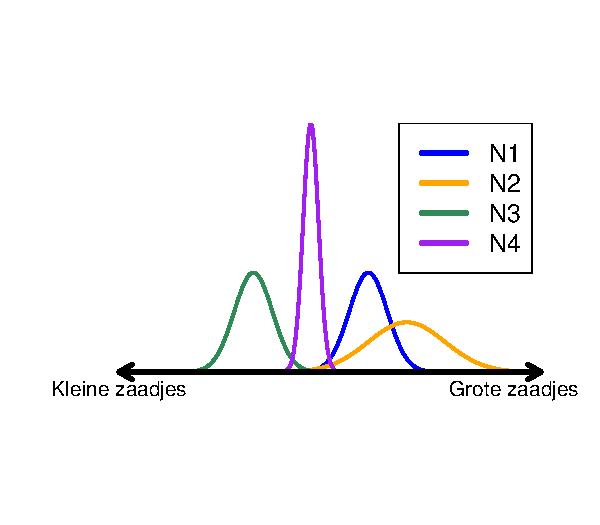
\includegraphics{Modellering/ecoevo_evolutiediversiteit_files/figure-pdf/fig-nicheoverlaps2-1.pdf}

}

}

\subcaption{\label{fig-nicheoverlaps2-1}Niche-overlap weergegeven als
normaalverdelingen}
\end{minipage}%
%
\begin{minipage}[t]{0.50\linewidth}

{\centering 

\raisebox{-\height}{

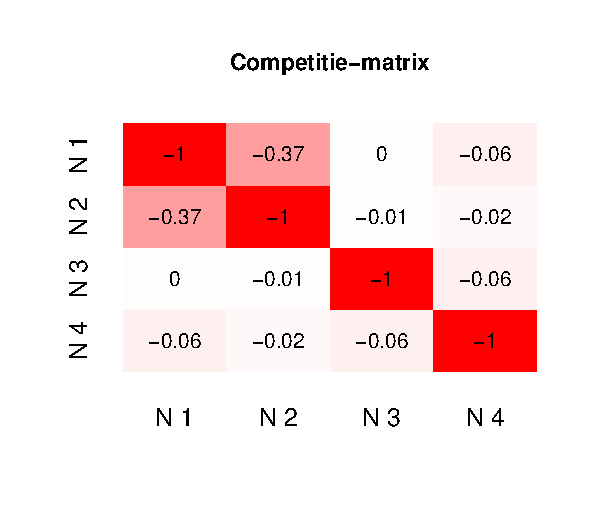
\includegraphics{Modellering/ecoevo_evolutiediversiteit_files/figure-pdf/fig-nicheoverlaps2-2.pdf}

}

}

\subcaption{\label{fig-nicheoverlaps2-2}Niche-overlap weergegeven als
een interactiematrix}
\end{minipage}%

\caption{\label{fig-nicheoverlaps2}Niche-overlap voor vier vogelsoorten
met een andere voorkeur voor de grootte van zaadjes, en ook met een
andere spreiding}

\end{figure}

Laten we eerst kijken hoe we het scenario met slechts 2 soorten kunnen
bestuderen (uit Figuur~\ref{fig-nicheoverlaps}). Hiervoor gebruiken we
ons eerdere competitie-model (Vergelijking~\ref{eq-soorten}) en stellen
de juiste parameters in in Grind:

\begin{Shaded}
\begin{Highlighting}[]
\CommentTok{\# Laad het grind.R{-}script in}
\FunctionTok{source}\NormalTok{(}\StringTok{"https://tbb.bio.uu.nl/rdb/grindR/grind.R"}\NormalTok{)}

\CommentTok{\# Definitie van model. Alleen de binnenste drie regels hoeven we }
\CommentTok{\# aan te passen. Het \textquotesingle{}function\textquotesingle{} en \textquotesingle{}with\textquotesingle{} gedeelte laten we staan}
\CommentTok{\# zoals het is. }
\NormalTok{model }\OtherTok{\textless{}{-}} \ControlFlowTok{function}\NormalTok{(t, state, parms) \{}
  \FunctionTok{with}\NormalTok{(}\FunctionTok{as.list}\NormalTok{(}\FunctionTok{c}\NormalTok{(state,parms)), \{}
\NormalTok{    dN1 }\OtherTok{\textless{}{-}}\NormalTok{ r}\SpecialCharTok{*}\NormalTok{N1}\SpecialCharTok{*}\NormalTok{(}\DecValTok{1}\SpecialCharTok{{-}}\NormalTok{c11}\SpecialCharTok{*}\NormalTok{N1}\SpecialCharTok{{-}}\NormalTok{c12}\SpecialCharTok{*}\NormalTok{N2)}
\NormalTok{    dN2 }\OtherTok{\textless{}{-}}\NormalTok{ r}\SpecialCharTok{*}\NormalTok{N2}\SpecialCharTok{*}\NormalTok{(}\DecValTok{1}\SpecialCharTok{{-}}\NormalTok{c22}\SpecialCharTok{*}\NormalTok{N2}\SpecialCharTok{{-}}\NormalTok{c21}\SpecialCharTok{*}\NormalTok{N1)}
    \FunctionTok{return}\NormalTok{(}\FunctionTok{list}\NormalTok{(}\FunctionTok{c}\NormalTok{(dN1, dN2)))  }
\NormalTok{  \}) }
\NormalTok{\}  }


\NormalTok{p }\OtherTok{\textless{}{-}} \FunctionTok{c}\NormalTok{(}\AttributeTok{r=}\DecValTok{1}\NormalTok{,}\AttributeTok{c11=}\DecValTok{1}\NormalTok{,}\AttributeTok{c22=}\DecValTok{1}\NormalTok{,}\AttributeTok{c12=}\FloatTok{0.32}\NormalTok{,}\AttributeTok{c21=}\FloatTok{0.32}\NormalTok{)  }\CommentTok{\#parameters}
\NormalTok{s }\OtherTok{\textless{}{-}} \FunctionTok{c}\NormalTok{(}\AttributeTok{N1=}\FloatTok{0.01}\NormalTok{,}\AttributeTok{N2=}\FloatTok{0.001}\NormalTok{) }\CommentTok{\# kleine begin{-}dichtheden}

\NormalTok{colors[}\DecValTok{1}\NormalTok{] }\OtherTok{=} \StringTok{"blue"}
\NormalTok{colors[}\DecValTok{2}\NormalTok{] }\OtherTok{=} \StringTok{"orange"}
\FunctionTok{par}\NormalTok{(}\AttributeTok{mfrow=}\FunctionTok{c}\NormalTok{(}\DecValTok{1}\NormalTok{,}\DecValTok{1}\NormalTok{),}\AttributeTok{mar=}\FunctionTok{c}\NormalTok{(}\DecValTok{4}\NormalTok{,}\DecValTok{4}\NormalTok{,}\DecValTok{2}\NormalTok{,}\DecValTok{2}\NormalTok{)) }\CommentTok{\# maak twee plot{-}ruimtes}
\FunctionTok{plane}\NormalTok{(}\AttributeTok{vector=}\NormalTok{T,}\AttributeTok{grid=}\DecValTok{4}\NormalTok{,}\AttributeTok{ymax=}\FloatTok{3.5}\NormalTok{,}\AttributeTok{xmax=}\FloatTok{3.5}\NormalTok{,}\AttributeTok{portrait=}\NormalTok{F) }\CommentTok{\# faseruimte }
\FunctionTok{newton}\NormalTok{(}\FunctionTok{c}\NormalTok{(}\AttributeTok{N1=}\DecValTok{1}\NormalTok{,}\AttributeTok{N2=}\DecValTok{1}\NormalTok{),}\AttributeTok{plot=}\NormalTok{T)}
\FunctionTok{newton}\NormalTok{(}\FunctionTok{c}\NormalTok{(}\AttributeTok{N1=}\DecValTok{0}\NormalTok{,}\AttributeTok{N2=}\DecValTok{1}\NormalTok{),}\AttributeTok{plot=}\NormalTok{T)}
\FunctionTok{newton}\NormalTok{(}\FunctionTok{c}\NormalTok{(}\AttributeTok{N1=}\DecValTok{1}\NormalTok{,}\AttributeTok{N2=}\DecValTok{0}\NormalTok{),}\AttributeTok{plot=}\NormalTok{T)}
\FunctionTok{newton}\NormalTok{(}\FunctionTok{c}\NormalTok{(}\AttributeTok{N1=}\DecValTok{0}\NormalTok{,}\AttributeTok{N2=}\DecValTok{0}\NormalTok{),}\AttributeTok{plot=}\NormalTok{T)}
\end{Highlighting}
\end{Shaded}

\begin{figure}[H]

{\centering 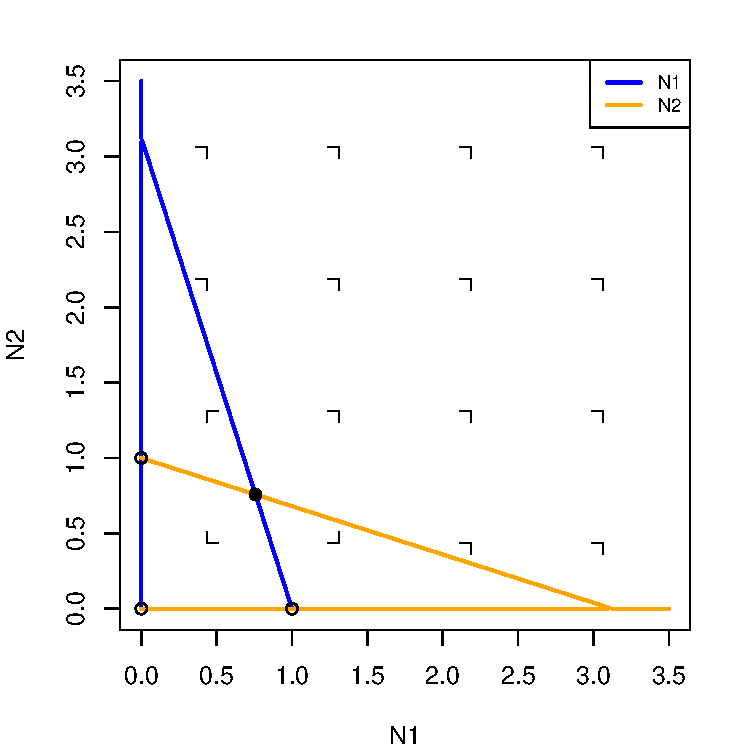
\includegraphics[width=0.7\textwidth,height=\textheight]{Modellering/ecoevo_evolutiediversiteit_files/figure-pdf/fig-grindoverlaps-1.pdf}

}

\caption{\label{fig-grindoverlaps}CAPTION TODO}

\end{figure}

Zoals je ziet resulteert dit in een stabiel evenwicht waarbij beide
soorten voorkomen. Wat nu als we het scenario uit
Figuur~\ref{fig-nicheoverlaps2} met 4 soorten willen bekijken? Hier
zouden we dan 4 ODEs met ieder 4 interactie-termen moeten gebruiken. Hoe
meer soorten je dus toevoegt, hoe groter de vergelijkingen worden
(bovendien is een faseruimte in 4D tekenen is zeer zeker geen optie).
Kan dat ook anders?

\hypertarget{interactie-matrixen-met-meerdere-soorten}{%
\section{Interactie-matrixen met meerdere
soorten}\label{interactie-matrixen-met-meerdere-soorten}}

Hoewel de matrices hierboven slechts competities beschreven, zouden er
ook positieve effecten in verwerkt kunnen worden. Algemener beschrijft
een dergelijke matrix dan de interactie tussen de soorten, vandaar de
naam interactie-matrix. Interactie-matrices hebben dus een hele concrete
biologische interpretatie: het vat samen welke positieve/negatieve
effecten soorten hebben op hun eigen dichtheid, en op de dichtheid van
de andere soorten. Dergelijke interacties kunnen experimenteel bepaald
worden, bijvoorbeeld door vele combinaties van bacteriën samen te laten
groeien, of simpelweg door eens in de zoveel jaar bij te houden hoe de
soortensamenstelling is verschoven.

Zo heeft Henry Horn bijvoorbeeld in 1975 precies bepaald hoe de
soortensamenstelling van bomen in een bos in Amerika was verschoven na
een periode van 50 jaar. Dit gaf hij weer in een simpele matrix:

\begin{longtable}[]{@{}lllll@{}}
\toprule\noalign{}
& Gray Birch & Blackgum & Red Maple & Beech \\
\midrule\noalign{}
\endhead
\bottomrule\noalign{}
\endlastfoot
Gray Birch & 0.05 & 0.01 & \& 0 & 0 \\
Blackgum & 0.36 & 0.57 & 0.14 & 0.01 \\
Red Maple & 0.5 & 0.25 & 0.55 & 0.03 \\
Beech & 0.09 & 0.17 & 0.31 & 0.96 \\
\end{longtable}

Deze matrix geeft, anders dan de eerder genoemde interactie-matrixen,
niet aan hoeveel ``last'' de soorten van elkaar hebben, maar welke soort
wordt opgevolgd door welke soort (we zouden het dus ook een
successie-matrix kunnen noemen). De details van deze ecologische
successie lees je af aan de kolommen. Kijk bijvoorbeeld naar de eerste
kolom: voor elke 100 \emph{Gray Birch} bomen meette hij 5 nieuwe
\emph{Gray Birch}, 36 nieuwe \emph{Blackgum}, 50 nieuwe \emph{Red
Maple}, en 9 nieuwe \emph{Beech} bomen. Als we beginnen met alleen maar
\emph{Gray Birch}, zouden we dat kunnen weergeven als een zogeheten
\emph{state vector}: \texttt{(100,0,0,0)}. Na 50 jaar is deze state
vector \texttt{(5,36,50,9)}. In de 50 jaar daarna, worden de 5
overgebleven \emph{Gray Birch} bomen wederom naar gelang hetzelfde
process vervangen. Maar let op: als je goed kijkt zie je dat ook 1\% van
de \emph{Blackgum} bomen ``terug verandert'' in \emph{Gray Birch}.
Tegelijkertijd zal 25\% van deze \emph{Blackgum} populatie vervangen
worden door \emph{Red Maple}, \emph{etc.}.

Als we herhaaldelijk de intearctie-matrix met onze state vector
vermenigvuldigen, wat kan met een simpel R-script (voor verdieping over
matrix-vector vermenigvuldiging, zie (\textbf{tip-vecmat?})), zien we
inderdaad een prachtige en welbekende successie van boomsoorten:
uiteindelijk zijn er vooral beuken over, en zie je geen berken meer.

\begin{Shaded}
\begin{Highlighting}[]
\NormalTok{A }\OtherTok{\textless{}{-}} 
  \FunctionTok{matrix}\NormalTok{(}\FunctionTok{c}\NormalTok{(}\FloatTok{0.05}\NormalTok{, }\FloatTok{0.01}\NormalTok{, }\DecValTok{0}\NormalTok{, }\DecValTok{0}\NormalTok{,}
           \FloatTok{0.36}\NormalTok{, }\FloatTok{0.57}\NormalTok{, }\FloatTok{0.14}\NormalTok{, }\FloatTok{0.01}\NormalTok{,}
           \FloatTok{0.5}\NormalTok{, }\FloatTok{0.25}\NormalTok{, }\FloatTok{0.55}\NormalTok{, }\FloatTok{0.03}\NormalTok{,}
           \FloatTok{0.09}\NormalTok{, }\FloatTok{0.17}\NormalTok{, }\FloatTok{0.31}\NormalTok{, }\FloatTok{0.96}\NormalTok{),}\AttributeTok{nrow=}\DecValTok{4}\NormalTok{,}\AttributeTok{byrow=}\NormalTok{T)}
\NormalTok{S }\OtherTok{\textless{}{-}} \FunctionTok{c}\NormalTok{(}\DecValTok{100}\NormalTok{,}\DecValTok{0}\NormalTok{,}\DecValTok{0}\NormalTok{,}\DecValTok{0}\NormalTok{)}
\NormalTok{succession }\OtherTok{\textless{}{-}} \FunctionTok{data.frame}\NormalTok{()}
\ControlFlowTok{for}\NormalTok{(i }\ControlFlowTok{in} \DecValTok{1}\SpecialCharTok{:}\DecValTok{20}\NormalTok{)}
\NormalTok{\{}
\NormalTok{  succession }\OtherTok{\textless{}{-}} \FunctionTok{rbind}\NormalTok{(succession, }\FunctionTok{t}\NormalTok{(S)) }\CommentTok{\# voeg nieuwe vector toe aan tijdlijn}
\NormalTok{  S }\OtherTok{\textless{}{-}}\NormalTok{ A }\SpecialCharTok{\%*\%}\NormalTok{ S }\CommentTok{\# R notatie voor matrix{-}vermenigvuldiging}
\NormalTok{\}}
\FunctionTok{library}\NormalTok{(DT)}
\FunctionTok{colnames}\NormalTok{(succession) }\OtherTok{\textless{}{-}} \FunctionTok{c}\NormalTok{(}\StringTok{"Birch"}\NormalTok{, }\StringTok{"Blackgum"}\NormalTok{, }\StringTok{"Red Maple"}\NormalTok{, }\StringTok{"Beech"}\NormalTok{)}
\FunctionTok{datatable}\NormalTok{(succession)}
\end{Highlighting}
\end{Shaded}

\begin{figure}[H]

{\centering 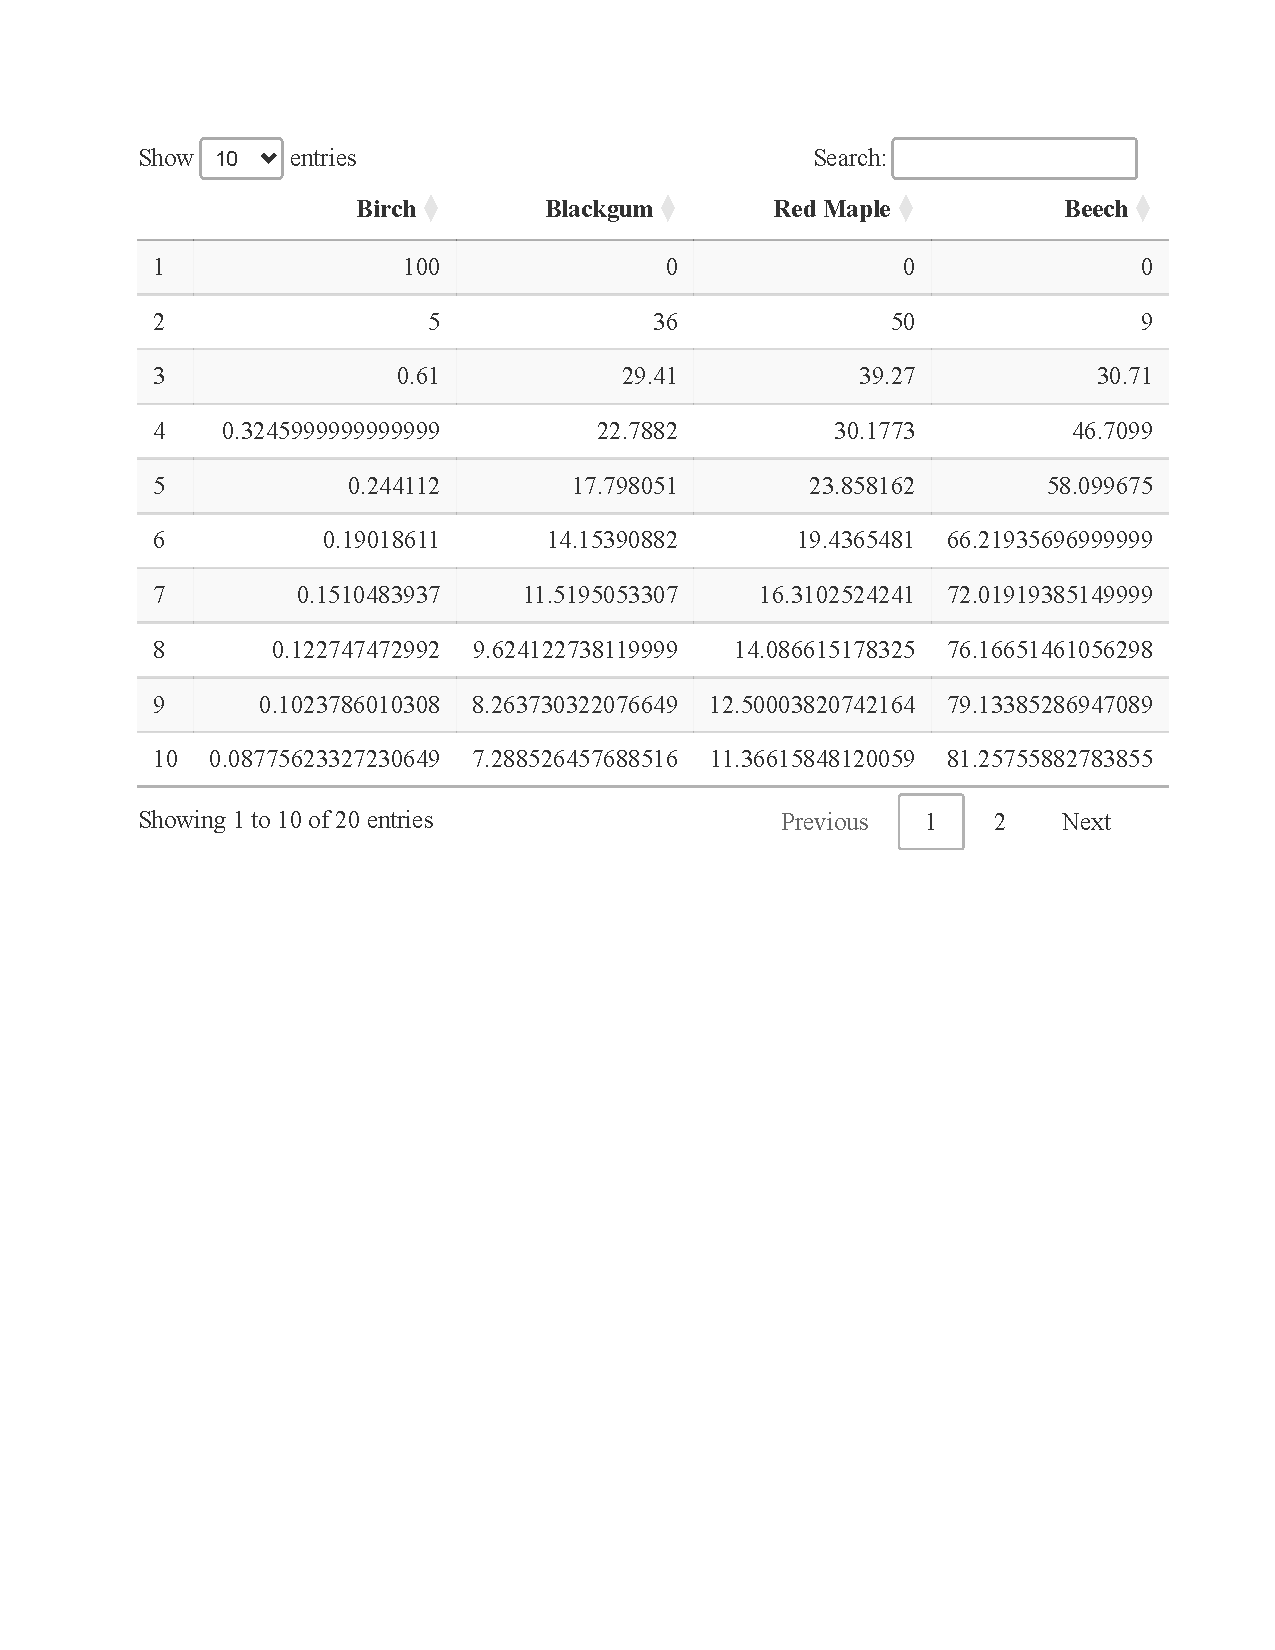
\includegraphics{Modellering/ecoevo_evolutiediversiteit_files/figure-pdf/unnamed-chunk-5-1.pdf}

}

\end{figure}

Ook met Grind kun je, op een vergelijkbare manier, een interactie-matrix
gebruiken om deze ecologische successie door te rekenen. In plaats van
steeds meer ODEs opschrijven, kunnen we het systeem ook opschrijen als
een hele verzameling van vergelijkingen waarin we een matrix (zie
verdieping in (\textbf{tip-vecmat?})) gebruiken om competitie van alle
te sommeren:

\begin{align}
\mathchoice{\frac{\mathrm{d}N_i}
{\mathrm{d}t}}{\mathrm{d}N_i/\mathrm{d}t}
{\mathrm{d}N_i/\mathrm{d}t}
{\mathrm{d}N_i/\mathrm{d}t} = rN_i \Big( 1 + \sum_{j=1}^n{A_{ij}N_i} \Big)
\end{align}

In Grind kun je ook dergelijke matrices gebruiken om in 1 klap een hele
boel ODEs door te rekenen:

\begin{Shaded}
\begin{Highlighting}[]
\CommentTok{\# Load necessary packages}
\FunctionTok{source}\NormalTok{(}\StringTok{"https://tbb.bio.uu.nl/rdb/grindR/grind.R"}\NormalTok{)}
\CommentTok{\# Set the seed for reproducibility}
\FunctionTok{set.seed}\NormalTok{(}\DecValTok{5}\NormalTok{)}

\CommentTok{\# Define the number of species}
\NormalTok{n\_species }\OtherTok{\textless{}{-}} \DecValTok{4}
\NormalTok{max\_time }\OtherTok{\textless{}{-}} \DecValTok{20}

\NormalTok{interaction\_matrix}\OtherTok{\textless{}{-}} \FunctionTok{matrix}\NormalTok{(}\FunctionTok{c}\NormalTok{(}\FloatTok{0.05}\NormalTok{, }\FloatTok{0.01}\NormalTok{, }\DecValTok{0}\NormalTok{, }\DecValTok{0}\NormalTok{,}
         \FloatTok{0.36}\NormalTok{, }\FloatTok{0.57}\NormalTok{, }\FloatTok{0.14}\NormalTok{, }\FloatTok{0.01}\NormalTok{,}
         \FloatTok{0.5}\NormalTok{, }\FloatTok{0.25}\NormalTok{, }\FloatTok{0.55}\NormalTok{, }\FloatTok{0.03}\NormalTok{,}
         \FloatTok{0.09}\NormalTok{, }\FloatTok{0.17}\NormalTok{, }\FloatTok{0.31}\NormalTok{, }\FloatTok{0.96}\NormalTok{),}\AttributeTok{nrow=}\DecValTok{4}\NormalTok{,}\AttributeTok{byrow=}\NormalTok{T)}

\CommentTok{\# Set up the layout for two plots side by side}
\FunctionTok{layout}\NormalTok{(}\FunctionTok{matrix}\NormalTok{(}\DecValTok{1}\SpecialCharTok{:}\DecValTok{1}\NormalTok{, }\AttributeTok{nrow =} \DecValTok{1}\NormalTok{), }\AttributeTok{widths =} \FunctionTok{c}\NormalTok{(}\DecValTok{1}\NormalTok{, }\DecValTok{1}\NormalTok{))  }\CommentTok{\# Adjust widths for better fit}
\FunctionTok{par}\NormalTok{(}\AttributeTok{mar=}\FunctionTok{c}\NormalTok{(}\DecValTok{5}\NormalTok{,}\DecValTok{4}\NormalTok{,}\DecValTok{3}\NormalTok{,}\DecValTok{3}\NormalTok{))}

\NormalTok{model }\OtherTok{\textless{}{-}} \ControlFlowTok{function}\NormalTok{(t, state, parms) \{}
\NormalTok{  N }\OtherTok{\textless{}{-}}\NormalTok{ state}
\NormalTok{  dN }\OtherTok{\textless{}{-}}\NormalTok{ interaction\_matrix }\SpecialCharTok{\%*\%}\NormalTok{ N }\SpecialCharTok{{-}}\NormalTok{ N}
  \FunctionTok{return}\NormalTok{(}\FunctionTok{list}\NormalTok{(dN))  }
\NormalTok{\}}
\NormalTok{p }\OtherTok{\textless{}{-}} \FunctionTok{c}\NormalTok{()}
\NormalTok{s }\OtherTok{\textless{}{-}} \FunctionTok{c}\NormalTok{(}\DecValTok{1}\NormalTok{,}\DecValTok{0}\NormalTok{,}\DecValTok{0}\NormalTok{,}\DecValTok{0}\NormalTok{)}
\FunctionTok{names}\NormalTok{(s) }\OtherTok{\textless{}{-}} \FunctionTok{c}\NormalTok{(}\StringTok{"Birch"}\NormalTok{,}\StringTok{"Blackgum"}\NormalTok{,}\StringTok{"Red maple"}\NormalTok{,}\StringTok{"Beech"}\NormalTok{)}
\NormalTok{colors[}\DecValTok{1}\NormalTok{] }\OtherTok{=} \StringTok{"\#00EE00"}
\NormalTok{colors[}\DecValTok{2}\NormalTok{] }\OtherTok{=} \StringTok{"\#00CC00"}
\NormalTok{colors[}\DecValTok{3}\NormalTok{] }\OtherTok{=} \StringTok{"\#00AA00"}
\NormalTok{colors[}\DecValTok{4}\NormalTok{] }\OtherTok{=} \StringTok{"\#008800"}

\FunctionTok{run}\NormalTok{(}\AttributeTok{tmax=}\NormalTok{max\_time,}\AttributeTok{legend=}\NormalTok{T,}\AttributeTok{tstep =} \FloatTok{0.1}\NormalTok{)}
\end{Highlighting}
\end{Shaded}

\begin{figure}[H]

{\centering 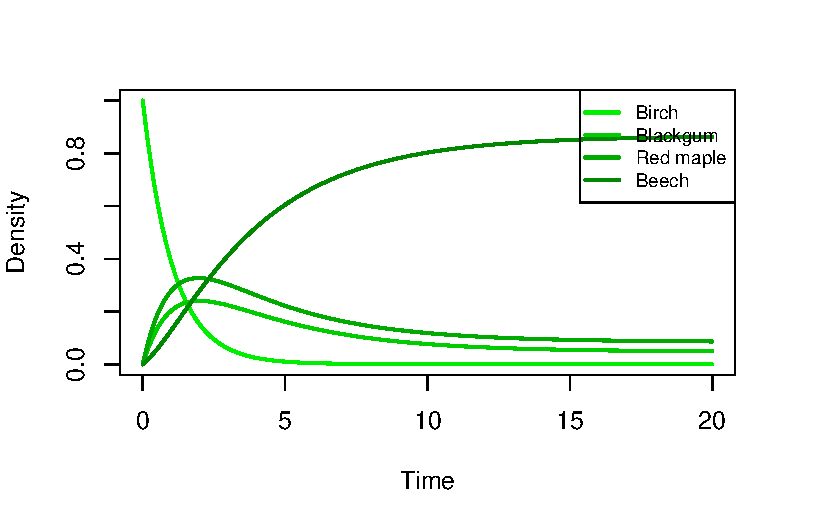
\includegraphics{Modellering/ecoevo_evolutiediversiteit_files/figure-pdf/unnamed-chunk-6-1.pdf}

}

\end{figure}

Of we kunnen in plaats van deze ecologische successie het Lotka-Volterra
competitie model uitbreiden naar een groot aantal soorten met
willekeurig gekozen parameters:

\begin{Shaded}
\begin{Highlighting}[]
\FunctionTok{source}\NormalTok{(}\StringTok{"https://tbb.bio.uu.nl/rdb/grindR/grind.R"}\NormalTok{)}
\FunctionTok{set.seed}\NormalTok{(}\DecValTok{12}\NormalTok{)}
\NormalTok{model }\OtherTok{\textless{}{-}} \ControlFlowTok{function}\NormalTok{(t, state, parms) \{}
\NormalTok{  N }\OtherTok{\textless{}{-}}\NormalTok{ state}
\NormalTok{  S }\OtherTok{\textless{}{-}}\NormalTok{ A }\SpecialCharTok{\%*\%}\NormalTok{ N }\CommentTok{\# R code for matrix x vector multiplication}
\NormalTok{  dN }\OtherTok{\textless{}{-}}\NormalTok{ r}\SpecialCharTok{*}\NormalTok{N}\SpecialCharTok{*}\NormalTok{(}\DecValTok{1} \SpecialCharTok{{-}}\NormalTok{ S)}
  \FunctionTok{return}\NormalTok{(}\FunctionTok{list}\NormalTok{(dN))  }
\NormalTok{\}  }

\NormalTok{p }\OtherTok{\textless{}{-}} \FunctionTok{c}\NormalTok{()}
\NormalTok{n }\OtherTok{\textless{}{-}} \DecValTok{30}
\NormalTok{s }\OtherTok{\textless{}{-}} \FunctionTok{rep}\NormalTok{(}\FloatTok{0.01}\NormalTok{,n)}
\FunctionTok{names}\NormalTok{(s) }\OtherTok{\textless{}{-}} \FunctionTok{paste}\NormalTok{(}\StringTok{"N"}\NormalTok{,}\FunctionTok{seq}\NormalTok{(}\DecValTok{1}\NormalTok{,n),}\AttributeTok{sep=}\StringTok{""}\NormalTok{)}
\NormalTok{r }\OtherTok{\textless{}{-}} \FunctionTok{abs}\NormalTok{(}\FunctionTok{rnorm}\NormalTok{(n,}\DecValTok{1}\NormalTok{,}\FloatTok{0.1}\NormalTok{))}
\NormalTok{A }\OtherTok{\textless{}{-}} \FunctionTok{matrix}\NormalTok{(}\FunctionTok{runif}\NormalTok{(n}\SpecialCharTok{*}\NormalTok{n),}\AttributeTok{nrow=}\NormalTok{n,}\AttributeTok{ncol=}\NormalTok{n)}
\FunctionTok{diag}\NormalTok{(A) }\OtherTok{\textless{}{-}} \DecValTok{1}\NormalTok{; A}

\FunctionTok{run}\NormalTok{(}\AttributeTok{tmax=}\DecValTok{300}\NormalTok{,}\AttributeTok{legend=}\NormalTok{F)}
\end{Highlighting}
\end{Shaded}

\begin{figure}[H]

{\centering 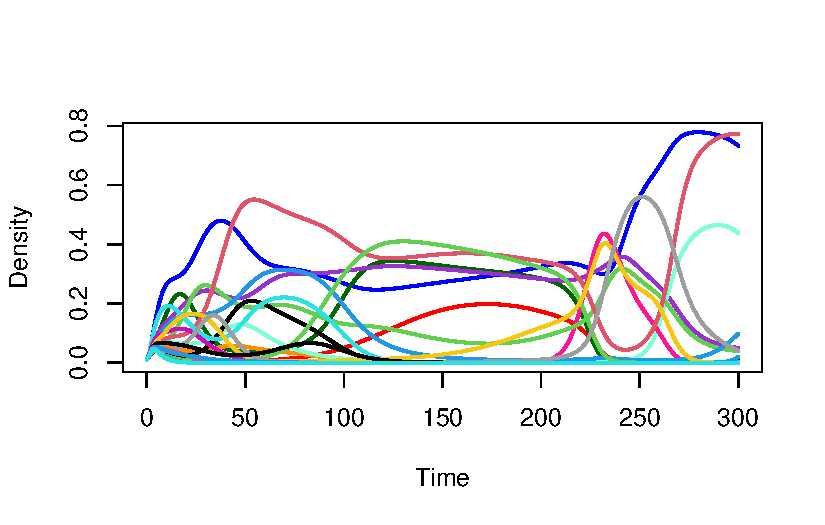
\includegraphics{Modellering/ecoevo_evolutiediversiteit_files/figure-pdf/unnamed-chunk-7-1.pdf}

}

\end{figure}

De details van het bovenstaande scripst zijn geen leerstof, maar het is
wel belangrijk dat je begrijpt waarom er vaak met matrices wordt gewerkt
om complexe modellen door te rekenen! Bovendien zie je al gauw dat het
moeilijk wordt om te voorspellen wie er in een complex ecosysteem
uiteindelijk zal overleven, omdat het systeem meerdere keren om lijkt te
slaan.

\begin{tcolorbox}[enhanced jigsaw, coltitle=black, breakable, bottomtitle=1mm, opacityback=0, colback=white, rightrule=.15mm, title=\textcolor{quarto-callout-tip-color}{\faLightbulb}\hspace{0.5em}{Vergelijkingen, vectoren, en matrices}, bottomrule=.15mm, toprule=.15mm, left=2mm, colframe=quarto-callout-tip-color-frame, toptitle=1mm, opacitybacktitle=0.6, titlerule=0mm, colbacktitle=quarto-callout-tip-color!10!white, leftrule=.75mm, arc=.35mm]

De 1D en 2D differentiaalvergelijkingen waar je tot nu toe over hebt
geleerd zijn onderdeel van lineaire algebra. Hoe groter stelsels van
vergelijkingen worden (3D, 10D, \emph{etc.}), hoe minder handig het is
om iedere vergelijking los op te schrijven. In plaats worden
vergelijkingen zoals\ldots{}

\begin{align}
x - 2y = −5 \\
2x + y = 10 
\end{align}

\ldots opgeschreven als een matrix-vector vermenigvuldiging:

\begin{equation}
\begin{pmatrix}
1 & -2\\
2 & 1
\end{pmatrix}
\begin{pmatrix}
x \\
y 
\end{pmatrix}
=
\begin{pmatrix}
-5 \\
10 
\end{pmatrix}
\end{equation}

Wiskundig gezien staat hier precies hetzelfde (gegeven de rekenregels om
vectoren en matrices te vermenigvuldigen). De vierkante matrix kunnen we
\(A\) noemen, en geeft alle interactie-coëfficiënten aan tussen x en y
(1, -2, 2, en 1). De eerste vector bevat de variabelen \(x\) en \(y\),
en wordt in deze context de ``state''-vector (\(\overrightarrow{S}\))
genoemd. Als laatste kunnen we de uitkomst-vector \(\overrightarrow{V}\)
noemen, en het systeem zo opschrijven:

\begin{align}
A \cdot \overrightarrow{S} = \overrightarrow{V}
\end{align}

Als je een matrix en een vector vermenigvuldigd krijg je inderdaad een
nieuwe vector. We zouden met behulp van lineaire algebra nu uit kunnen
rekenen wat \(\overrightarrow{S}\) is, maar dat valt zeer zeker niet
onder de stof van deze cursus. Bovendien kun je ODEs alleen in simpele
matrix-vector vermenigvuldigingen vertalen als alle interactie lineair
zijn, wat lang niet altijd opgaat!

\end{tcolorbox}

\hypertarget{de-eerste-cooperators}{%
\section{De eerste cooperators}\label{de-eerste-cooperators}}

Hoewel niche-overlap een belangrijk component is van hoe soorten
competitie met elkaar ondervinden, heeft het ook zijn beperkingen. Het
kan bijvoorbeeld zo zijn dat de dichtheden van de populaties een effect
hebben op de interactie-matrix zélf. Dit laatste is het geval bij
cooperatie, waar we het in eerdere hoofdstukken al kort over hebben
gehad. Omdat cooperatie desalnietemin een evolutionair interssant
onderwerp is, gaan we dit verder bestuderen met simpele 2D ODEs en
\emph{Individual Based Models}.

Coöperatie komt in allerlei vormen voor: bevers bouwen samen dammen,
bijen vallen samen een indringer aan, en bacteriën scheiden enzymen die
polysacchariden afbreken, \emph{etc.} Maar voor nu laten we deze
biologische details weg, en vragen we een fundamentelere vraag: hoe kan
dergelijke coöperatie evolutionair gezien ontstaan, als er aan het begin
niemand is om mee samen te werken? De eerste ``samenwerkende'' mutant is
per definitie alleen, en zal dus ook geen evolutionair voordeel hebben
van dit gedrag. Dit wordt ook wel \textbf{dichtheidsafhankelijke
fitness} (\emph{density dependent fitness}) genoemd. Laten we ons
eerdere model van coöperatie nog een keer bekijken:

\begin{align*}
\mathchoice{\frac{\mathrm{d}C}
{\mathrm{d}t}}{\mathrm{d}C/\mathrm{d}t}
{\mathrm{d}C/\mathrm{d}t}
{\mathrm{d}C/\mathrm{d}t} &= bC^2(1-\frac{C}{K}) - dC
\end{align*}

De kwadratische term in deze ODE veroorzaakt coöperatieve groei: bij
kleine dichtheden (\(C<1\)) groeit de populatie langzamer dan zonder
coöperatie, want een getal kleiner dan \(1\) kwadrateren maakt dit getal
kleiner. Bij hogere dichtheden (\(C>1\)) zorgt kwadrateren juist voor
een verhoging, dus zal de populatie juist sneller groeien dan zonder
coöperatie. Dit zie je ook heel goed als we het faseportret van dit
coöperatieve groeimodel vergelijken met die van normale, logistische
groei:

\begin{figure}

{\centering 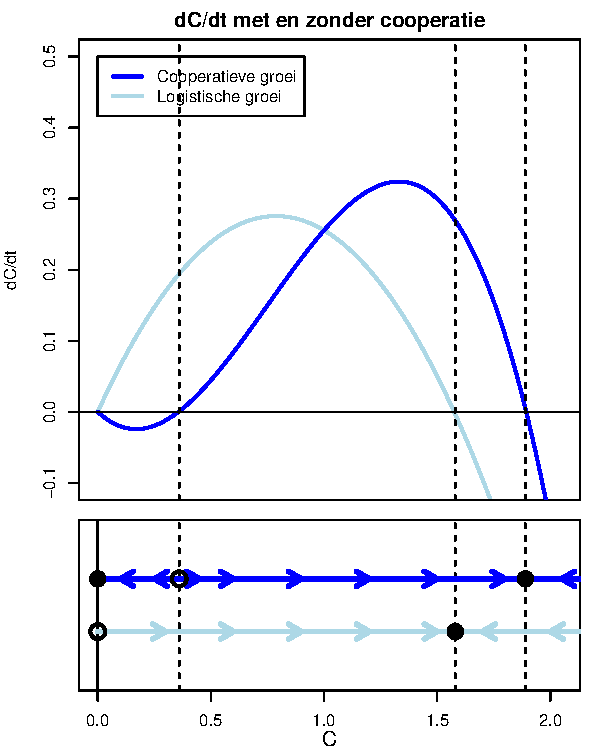
\includegraphics[width=4.5in,height=\textheight]{Modellering/ecoevo_evolutiediversiteit_files/figure-pdf/fig-coopphase-1.pdf}

}

\caption{\label{fig-coopphase}CAPTION TODO}

\end{figure}

Aan dit faseportret kunnen we een aantal belangrijke dingen aflezen. Ten
eerste zien we dat coöperatieve groei een hogere maximale groeisnelheid
heeft (de piek ligt hoger). Ten tweede zien we dat coöperatieve groei
ook een hogere \emph{carrying capacity} heeft, een dichtheid waarbij de
niet-coöperatieve soort alleen kan afnemen! Hoewel deze twee observaties
in het voordeel van de coöperatieve populatie spreken, zien we ook dat
reguliere logistische groei het juist veel beter doet bij \emph{lage}
dichtheden. Sterker nog, bij zeer lage dichtheden kunnen de coöperators
helemaal niet groeien, en de niet-coöperators wel! In plaats van deze
twee soorten als aparte populaties te bekijken, zouden we ze ook samen
kunnen brengen in een systeem van twee ODEs:

\begin{align*}
\mathchoice{\frac{\mathrm{d}C}
{\mathrm{d}t}}{\mathrm{d}C/\mathrm{d}t}
{\mathrm{d}C/\mathrm{d}t}
{\mathrm{d}C/\mathrm{d}t} &= bC^2(1-\frac{C+N}{K}) - dC\\
\mathchoice{\frac{\mathrm{d}N}
{\mathrm{d}t}}{\mathrm{d}N/\mathrm{d}t}
{\mathrm{d}N/\mathrm{d}t}
{\mathrm{d}N/\mathrm{d}t} &= bN(1-\frac{C+N}{K}) - dN
\end{align*}

Hier zijn \(C\) de cooperators, \(N\) de niet-cooperators, geeft \(b\)
de maximale birth rate, \(d\) de constante death rate, en \(K\) de
(gedeelde) carrying capacity. Kunnen deze twee soorten samenleven? Om
dit te bestuderen, kunnen we weer Grind gebruiken om een faseruimte te
plotten:

\begin{figure}

{\centering 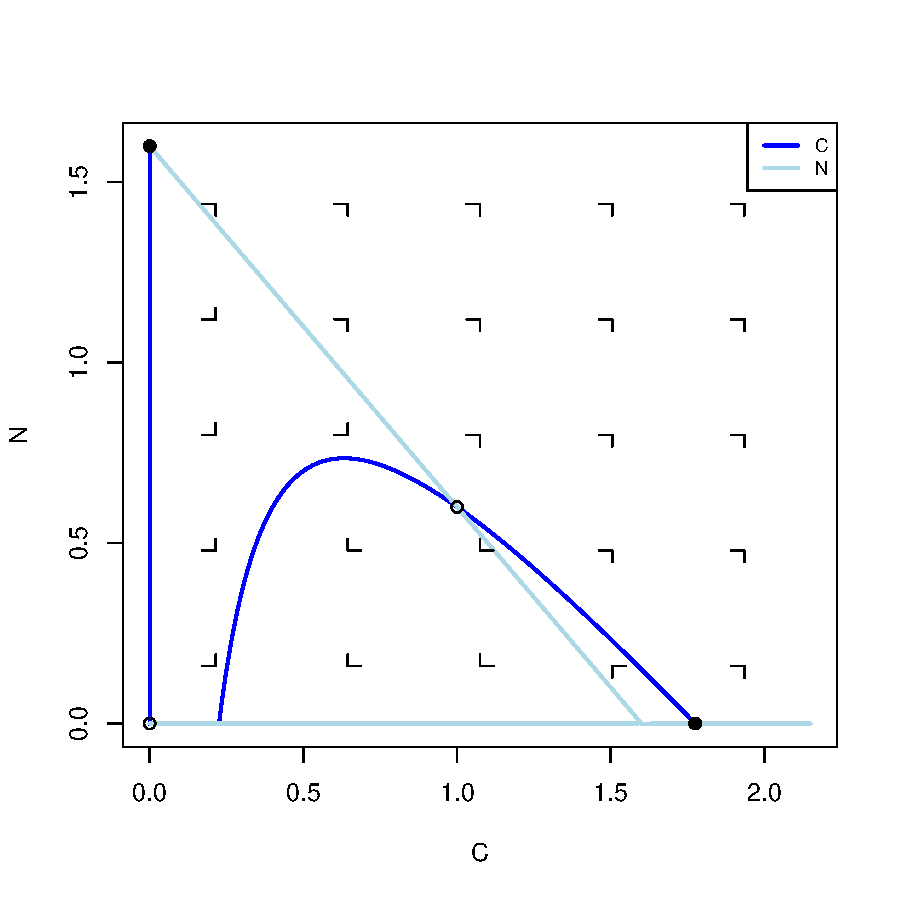
\includegraphics{Modellering/ecoevo_evolutiediversiteit_files/figure-pdf/fig-coopnoncoopgrind-1.pdf}

}

\caption{\label{fig-coopnoncoopgrind}CAPTION TODO}

\end{figure}

Zoals je ziet heeft het systeem twee stabiele evenwichtspunten
(aangegeven met gevulde punten). Er is een attractor voor veel \(C\) en
\(N=0\), maar ook één voor veel \(N\) en \(C=0\). Het evenwicht waar
zowel \(N\) als \(C\) bestaan is een zadelpunt: een instabiel evenwicht
waar het systeem uiteindelijk linksom of rechtsom van weggeduwd wordt.

Aan de hand van deze faseruimte kunnen we evolutionaire vragen stellen.
Stel je bijvoorbeeld voor dat we een populatie hebben van
niet-cooperators (het stabiele evenwicht linksbovenin). Door mutaties
kunnen cooperators onstaan, dus zullen we een klein stukje van dit
evenwicht weggeduwd worden (naar rechts). Maar vanaf hier zien we dat we
terug gaan naar het evenwicht van alleen niet-cooperators. Het
tegenovergestelde effect is ook zichtbaar: in een populatie van
cooperators kunnen niet-cooperators niet invaderen. Deze situatie,
waarbij een reeds gevestigde populatie voorkomt dat een andere soort kan
invaderen, wordt \emph{founder control} genoemd.

Uit de faseruimte hebben we dus geleerd dat vanuit een niet-cooperatieve
populatie geen coöperatie evolueren. Dit lijkt erg vreemd. We zien in de
natuur toch allerlei vormen van coöperatie?

\hypertarget{evolutie-van-cooperatie-in-ruimtelijke-modellen}{%
\section{Evolutie van cooperatie in ruimtelijke
modellen}\label{evolutie-van-cooperatie-in-ruimtelijke-modellen}}

In eerdere hoofdstukken hebben we ODEs vergeleken met ruimtelijke
modellen. Ook van deze situatie kunnen we een ruimtelijk model maken, om
te bestuderen of we verschillen zien:

Om te controleren dat het spatiele model overeenkomt met de ODE,
simuleert deze eerst perfect gemengde condities. Zoals je ziet komt ons
resultaat overeen met de ODEs: cooperators kunnen niet uitbreiden in een
populatie van niet-cooperators. Als we echter het experiment herhalen
met ruimtelijke structuur, zien we dat een kleine hoeveelheid
cooperators weldegelijk kan verspreiden:

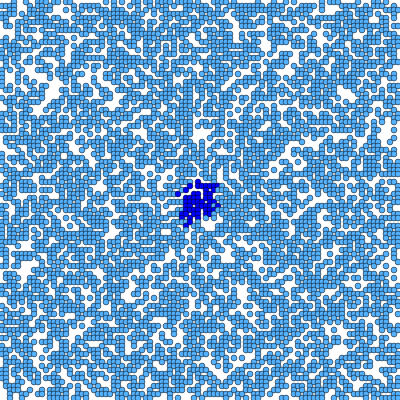
\includegraphics[width=0.32\textwidth,height=\textheight]{Modellering/figuren/coopspread1.png}
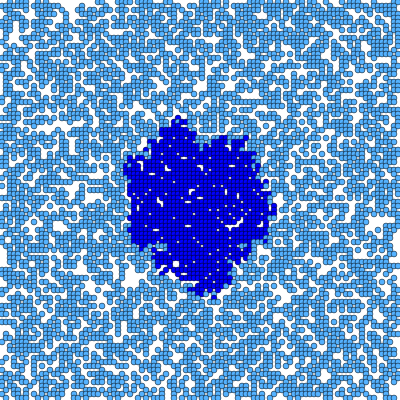
\includegraphics[width=0.32\textwidth,height=\textheight]{Modellering/figuren/coopspread2.png}
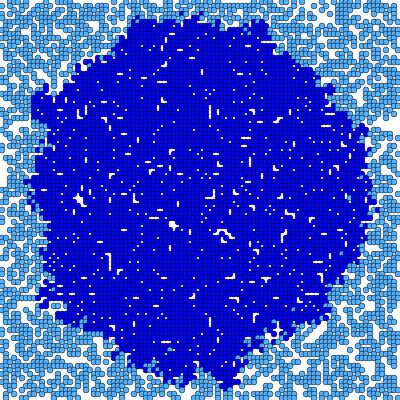
\includegraphics[width=0.32\textwidth,height=\textheight]{Modellering/figuren/coopspread3.png}

Waarom kan de cooperator nu wel verspreiden, als deze aanvankelijk een
lage dichtheid heeft? De reden hiervoor is simpel: in dit ruimtelijke
model is niet de \emph{globale} dichtheid relevant, maar de
\emph{lokale} dichtheid! Eén cooperator kan met een kleine hoeveelheid
cooperators samenwerken, en zo stap voor stap alle niet-cooperators
vervangen.

Omdat we nu te maken hebben met een \emph{individual-based model},
kunnen we wederom na gaan denken over \emph{individuele} regels. In
plaats van alleen ``cooperators'' en ``niet-cooperators'' te definiëren,
zouden we bijvoorbeeld ook de mate van cooperatie per individu kunnen
definieren, en deze eigenschap laten ``evolueren'' (bij elke
voortplanting vindt met een kleine kans een mutatie plaats). Zo ontstaat
er natuurlijk een diverse populatie:

In deze simulatie vinden ecologie en evolutie tegelijkertijd plaats, wat
ook wel ``eco-evolutionaire dynamica'' wordt genoemd. Hoewel ecologie en
evolutie vroeger vaak als twee aparte onderwerpen bestudeerd werden,
weten we nu dat deze processen elkaar sterk beinvloeden. Simulaties
zoals hierboven, waarin door een mutatie-proces nieuwe varianten
ontstaan, kunnen hulp bieden bij het begrijpen (en dus voorspellen!) van
kanker, antimicrobiële resistentie, en ziekte-verspreiding in de
landbouw.

Hoewel je bovenstaande simulaties ``voor de leuk'' even kan bestuderen,
is het geen leerstof. Het is echter heel belangrijk dat je begrijpt dat
het nuttig kan zijn hetzelfde fenomeen (hier: cooperatie) in
verschillende modelvormen te bestuderen, omdat de conclusies zeker niet
altijd hetzelfde zijn. Ruimtelijke modellen hebben, bijna zonder
uitzondering, altijd een andere uitkomst dan simpele ODEs. Dat betekent
niet dat één van de modellen ``fout'' is, maar dat we dus conclusies
kunnen trekken over de invloed van ruimtelijke structuur!

\hypertarget{mini-project}{%
\section{Mini-project}\label{mini-project}}

Voor dit hoofdstuk zijn geen opgaven. In plaats daarvan gaan jullie in
groepjes van 3 werken aan een mini-project, en schrijf je samen een kort
verslag. Dit verslag dient de volgende vorm te hebben:

\begin{itemize}
\tightlist
\item
  Een korte introductie (\textasciitilde200 woorden)
\item
  Stapsgewijs antwoorden op de vragen (a=\ldots, b=\ldots, etc.).
\item
  Een korte conclusie (1-2 zinnen)
\end{itemize}

Let bij het schrijven van je verslag op de volgende punten:

\begin{itemize}
\tightlist
\item
  Zorg dat uit je antwoord blijkt wat de vraag was! De vraag ``Welk
  effect heeft het verhogen van de carrying capacity van de konijnen op
  de hoeveelheid konijnen in evenwicht?'', beantwoord je zo: ``Het
  verhogen van de carrying capacity van de konijnen heeft geen invloed
  op de hoeveelheid konijnen in evenwicht. Dit komt doordat\ldots{}''
\item
  Ondersteun je antwoord met figuren, vooral wanneer hier expliciet om
  wordt gevraagd! Voor een schets kun je een foto maken van een vel
  papier (als deze maar duidelijk is. Voor plaatjes uit R en
  computer-simulaties kun je een natuurlijk gewoon een printscreen
  maken.
\end{itemize}

Succes met de opdracht!

\begin{tcolorbox}[enhanced jigsaw, coltitle=black, breakable, bottomtitle=1mm, opacityback=0, colback=white, rightrule=.15mm, title=\textcolor{quarto-callout-caution-color}{\faFire}\hspace{0.5em}{Computerpracticum over toxine-productie}, bottomrule=.15mm, toprule=.15mm, left=2mm, colframe=quarto-callout-caution-color-frame, toptitle=1mm, opacitybacktitle=0.6, titlerule=0mm, colbacktitle=quarto-callout-caution-color!10!white, leftrule=.75mm, arc=.35mm]

Verschillende bacteriën die in eenzelfde omgeving groeien ondergaan vele
interacties met elkaar. Naast het concurreren om voedsel, kunnen sommige
bacteriën ook giftige stoffen (toxines) uitscheiden om hun concurrenten
te onderdrukken. Sommige bacteriën scheiden deze toxines uit in het
medium, terwijl andere de toxines direct in hun buurcellen kunnen
injecteren. Hoewel dit deze bacteriën kan bevoordelen, dragen ze ook de
metabolische kosten voor het produceren van de toxines (en de
resistentie daartegen!). Om de ecologie van toxineproducenten te
bestuderen, hebben we een systeem van ODEs opgesteld dat twee stammen
beschrijft -- een toxineproducerende stam die resistent is tegen het
toxine en een gevoelige die dood gaat naar mate er meer
toxine-producenten aanwezig zijn:

\begin{align}
\mathchoice{\frac{\mathrm{d}X}
{\mathrm{d}t}}{\mathrm{d}X/\mathrm{d}t}
{\mathrm{d}X/\mathrm{d}t}
{\mathrm{d}X/\mathrm{d}t} &= a_{1}X(1-\frac{X+Y}{K}) - dX \\
\mathchoice{\frac{\mathrm{d}Y}
{\mathrm{d}t}}{\mathrm{d}Y/\mathrm{d}t}
{\mathrm{d}Y/\mathrm{d}t}
{\mathrm{d}Y/\mathrm{d}t} &= a_{2}Y(1-\frac{X+Y}{K}) - dY - cXY
\end{align}

\begin{enumerate}
\def\labelenumi{\alph{enumi}.}
\tightlist
\item
  Welke ODE (dX of dY) stelt de toxine-producerende stam voor, en welke
  de sensitieve stam? \emph{X is producent}
\item
  Gegeven de biologische context, waar staan de parameters \(a1\),
  \(a2\), \(K\), \(d\) en \(c\) voor?
\item
  We gaan ervan uit dat er metabolische kosten zijn voor de productie
  van toxines, maar dat sensitieven behoorlijk gevoelig zijn voor deze
  toxines. Verwachten dat een toxine-producerende mutant kan invaderen?
  \emph{Ja, je zou verwachten van wel (gegeven het woord `behoorlijk'),
  want de tweede soort een extra negatieve term heeft, de we net
  `behoorlijk' hebben genoemd xD!}
\item
  Bereken de nullclines van dit systeem. \emph{todo}
\item
  Schets de nullclines die je hebt gevonden in c.~Schets als het nodig
  is verschillende scenarios. Geef ook het vectorveld en de stabiliteit
  van de evenwichten weer. \emph{todo}
\item
  Beschrijf de gevonden evenwichten in biologische begrippen. Kan een
  toxine-producerende mutant (met lage metabolische kosten) invaderen in
  een populatie van sensitieven? \emph{nee, er is een zadelpunt
  evenwicht waardoor er sprake is van founder control (hebben ze dit
  hoofdstuk over geleerd)} Neem het volgende Grind-script over:
\end{enumerate}

\begin{Shaded}
\begin{Highlighting}[]
\FunctionTok{source}\NormalTok{(}\StringTok{"https://tbb.bio.uu.nl/rdb/grindR/grind.R"}\NormalTok{)}
\end{Highlighting}
\end{Shaded}

\begin{verbatim}
grind.R (25-06-2024) was sourced
\end{verbatim}

\begin{Shaded}
\begin{Highlighting}[]
\NormalTok{model }\OtherTok{\textless{}{-}} \ControlFlowTok{function}\NormalTok{(t, state, parms)\{}
  \FunctionTok{with}\NormalTok{(}\FunctionTok{as.list}\NormalTok{(}\FunctionTok{c}\NormalTok{(state,parms)),\{}
\NormalTok{    dX }\OtherTok{\textless{}{-}}\NormalTok{ a1}\SpecialCharTok{*}\NormalTok{X}\SpecialCharTok{*}\NormalTok{(}\DecValTok{1}\SpecialCharTok{{-}}\NormalTok{(X}\SpecialCharTok{+}\NormalTok{Y)}\SpecialCharTok{/}\NormalTok{K) }\SpecialCharTok{{-}}\NormalTok{ d}\SpecialCharTok{*}\NormalTok{X}
\NormalTok{    dY }\OtherTok{\textless{}{-}}\NormalTok{ a2}\SpecialCharTok{*}\NormalTok{Y}\SpecialCharTok{*}\NormalTok{(}\DecValTok{1}\SpecialCharTok{{-}}\NormalTok{(X}\SpecialCharTok{+}\NormalTok{Y)}\SpecialCharTok{/}\NormalTok{K) }\SpecialCharTok{{-}}\NormalTok{ d}\SpecialCharTok{*}\NormalTok{Y }\SpecialCharTok{{-}}\NormalTok{ c}\SpecialCharTok{*}\NormalTok{X}\SpecialCharTok{*}\NormalTok{Y}
    \FunctionTok{return}\NormalTok{(}\FunctionTok{list}\NormalTok{(}\FunctionTok{c}\NormalTok{(dX,dY)))}
\NormalTok{  \})}
\NormalTok{\}  }

\NormalTok{colors[}\DecValTok{1}\NormalTok{] }\OtherTok{=} \StringTok{"navy"}
\NormalTok{colors[}\DecValTok{2}\NormalTok{] }\OtherTok{=} \StringTok{"red"}

\NormalTok{p }\OtherTok{\textless{}{-}} \FunctionTok{c}\NormalTok{(}\AttributeTok{a1=}\FloatTok{0.6}\NormalTok{,}\AttributeTok{a2=}\FloatTok{1.0}\NormalTok{,}\AttributeTok{d=}\FloatTok{0.1}\NormalTok{,}\AttributeTok{c=}\FloatTok{0.5}\NormalTok{,}\AttributeTok{K=}\DecValTok{1}\NormalTok{)}
\NormalTok{s }\OtherTok{\textless{}{-}} \FunctionTok{c}\NormalTok{(}\AttributeTok{X=}\FloatTok{0.0001}\NormalTok{,}\AttributeTok{Y=}\FloatTok{0.9}\NormalTok{)}
\FunctionTok{par}\NormalTok{(}\AttributeTok{mfrow=}\FunctionTok{c}\NormalTok{(}\DecValTok{1}\NormalTok{,}\DecValTok{3}\NormalTok{))}
\FunctionTok{plane}\NormalTok{(}\AttributeTok{vector=}\NormalTok{T,}\AttributeTok{grid=}\DecValTok{3}\NormalTok{,}\AttributeTok{ymax=}\FloatTok{1.1}\NormalTok{,}\AttributeTok{xmax=}\FloatTok{1.1}\NormalTok{,}\AttributeTok{tstep=}\FloatTok{0.1}\NormalTok{, }\AttributeTok{portrait=}\NormalTok{T, }\AttributeTok{main=}\StringTok{"Totale faseruimte"}\NormalTok{)}
\FunctionTok{plane}\NormalTok{(}\AttributeTok{vector=}\NormalTok{T,}\AttributeTok{grid=}\DecValTok{6}\NormalTok{,}\AttributeTok{ymax=}\FloatTok{0.85}\NormalTok{,}\AttributeTok{ymin=}\FloatTok{0.6}\NormalTok{,}\AttributeTok{xmax=}\FloatTok{0.25}\NormalTok{, }\AttributeTok{xmin=}\FloatTok{0.05}\NormalTok{, }\AttributeTok{portrait=}\NormalTok{F, }\AttributeTok{main=}\StringTok{"(ingezoomed)"}\NormalTok{)}
\FunctionTok{newton}\NormalTok{(}\AttributeTok{state=}\FunctionTok{c}\NormalTok{(}\AttributeTok{X=}\FloatTok{0.15}\NormalTok{,}\AttributeTok{Y=}\FloatTok{0.7}\NormalTok{),}\AttributeTok{plot=}\NormalTok{T)}
\end{Highlighting}
\end{Shaded}

\begin{verbatim}
        X         Y 
0.1333337 0.6999995 
Saddle point (unstable), eigenvalues:
[1] -0.81438166  0.03438206
\end{verbatim}

\begin{verbatim}
        X         Y 
0.1333337 0.6999995 
\end{verbatim}

\begin{Shaded}
\begin{Highlighting}[]
\FunctionTok{run}\NormalTok{(}\AttributeTok{tmax=}\DecValTok{400}\NormalTok{,}\AttributeTok{traject=}\NormalTok{F, }\AttributeTok{main=}\StringTok{"Invasie van X"}\NormalTok{)}
\end{Highlighting}
\end{Shaded}

\begin{figure}[H]

{\centering 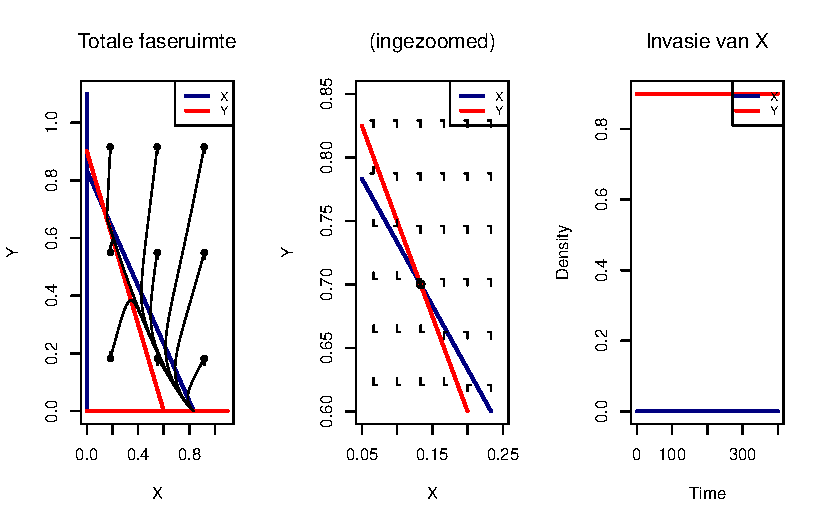
\includegraphics{Modellering/ecoevo_evolutiediversiteit_files/figure-pdf/unnamed-chunk-10-1.pdf}

}

\end{figure}

\begin{verbatim}
           X            Y 
1.378997e-11 9.000000e-01 
\end{verbatim}

\begin{enumerate}
\def\labelenumi{\alph{enumi}.}
\setcounter{enumi}{5}
\tightlist
\item
  Bestudeer met de parameters gegeven in het R-script of een
  toxine-producerende mutant zich kan verspreiden in een populatie van
  sensitieve cellen.
\item
  Verandert je antwoord in f als je de toxines 2 keer zo sterk maakt? En
  als je de toxines 10 keer zo sterk maakt?
\item
  Bestudeer ook of een sensitieve cell zich kan verspreiden in een
  populatie van toxine-producerende cellen. Wat als je de toxines 2 keer
  zo sterk maakt?
\item
  Trek uit de bovenstaande analyses een biologische conclusie.
  \emph{toxineproducent kan niet invaderen}
\end{enumerate}

De ODEs nemen aan dat het systeem goed gemengd is, zoals in een
Erlenmeyer die goed wordt geschud. Laten we ons virtuele experiment ook
herhalen op het equivalent van een agar-plaat, waar zowel reproductie
als de effecten van de toxines \emph{lokaal} zijn.

De parameters in de simulatie hebben vergelijkbare interpretaties als in
de ODEs. In de simulatie is er echter geen sprake van \emph{snelheden}
van geboorte en sterfte, maar \emph{kansen} van geboorte en sterfte.

\begin{figure}[H]

{\centering 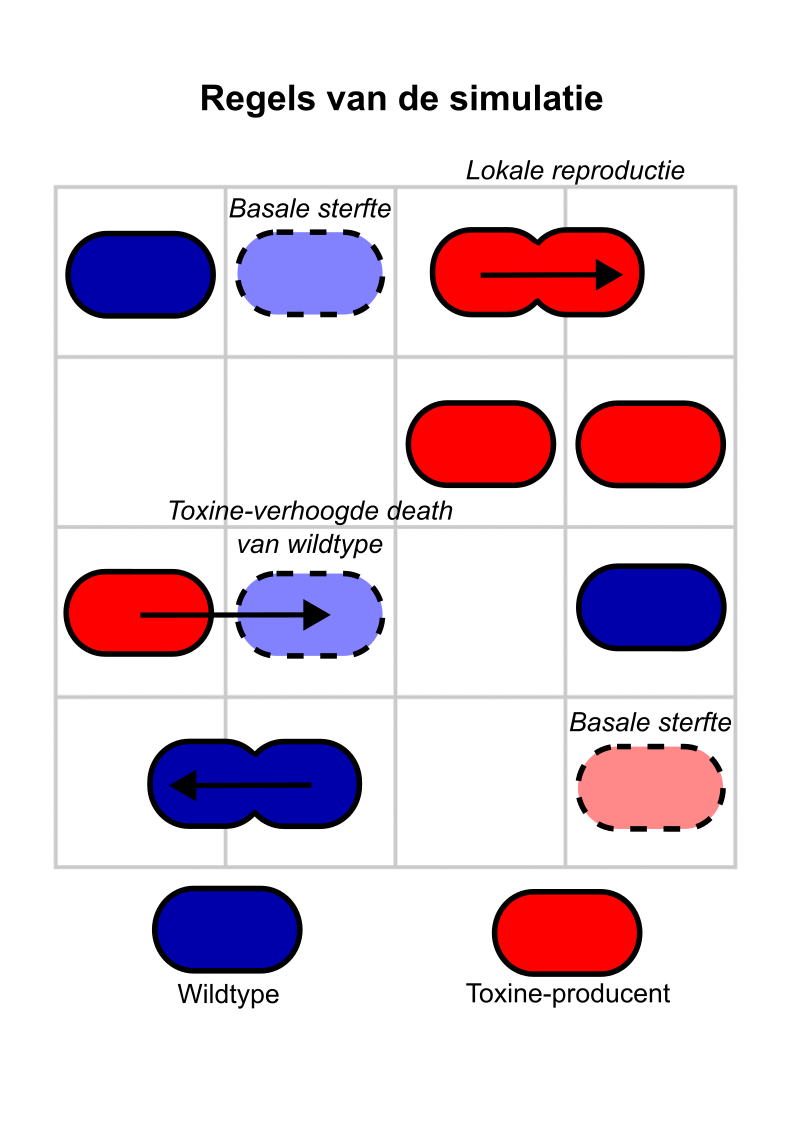
\includegraphics[width=0.6\textwidth,height=\textheight]{Modellering/figuren/project_toxins.png}

}

\end{figure}

Je vindt de simulatie hier:
\url{https://tbb.bio.uu.nl/bvd/bms/simulations/toxins/}

\begin{enumerate}
\def\labelenumi{\alph{enumi}.}
\setcounter{enumi}{9}
\tightlist
\item
  Bestudeer met de standaard parameters of de toxine-producent kan
  invaderen, en vorm een hypothese over wat er gebeurt
\item
  Test je hypothese met de opties die beschikbaar zijn in de simulatie.
\end{enumerate}

Vergeet niet te eindigen met een \emph{algemene conclusie}!

\end{tcolorbox}

\begin{longtable}[]{@{}
  >{\raggedright\arraybackslash}p{(\columnwidth - 4\tabcolsep) * \real{0.2500}}
  >{\raggedright\arraybackslash}p{(\columnwidth - 4\tabcolsep) * \real{0.2778}}
  >{\raggedright\arraybackslash}p{(\columnwidth - 4\tabcolsep) * \real{0.4722}}@{}}
\toprule\noalign{}
\begin{minipage}[b]{\linewidth}\raggedright
Nederlands
\end{minipage} & \begin{minipage}[b]{\linewidth}\raggedright
Engels
\end{minipage} & \begin{minipage}[b]{\linewidth}\raggedright
Beschrijving
\end{minipage} \\
\midrule\noalign{}
\endhead
\bottomrule\noalign{}
\endlastfoot
Interactie-matrix & Interaction matrix & Een matrix (tabel) die de alle
interacties tussen de soorten aangeeft. \\
Competitie-matrix & Competition matrix & Een matrix (tabel) die de alle
competitie-interacties tussen de soorten aangeeft. \\
Successie-matrix & Succession matrix & Een matrix (tabel) die de
aangeeft welke soort wordt opgevolgd door welke soort. \\
Eco-evolutionary dynamica & Eco-evolutionary dynamics & Biologische
dynamica waarin ecologie en evolutie tegelijkertijd afspelen, waardoor
er een wisselwerking kan zijn tussen beiden. \\
Dichtheidsafhankelijke fitness & Density dependent fitness & Wanneer de
fitness van een soort afhangt van zijn eigen dichtheid, bijvoorbeeld
wanneer er sprake is van samenwerking die bij lage dichtheden niet
uitpakt. \\
Eco-evolutionary dynamica & Eco-evolutionary dynamics & Biologische
dynamica waarin ecologie en evolutie tegelijkertijd afspelen, waardoor
er een wisselwerking kan zijn tussen beiden. \\
Lokale/globale dichtheid & Local/global density & De lokale dichtheid
geeft aan hoeveel individuen er in de directe omgeving van een bepaald
individu aanwezig zijn. Dit wordt vaak gemeten binnen een specifieke
straal rondom het individu. De globale dichtheid beschrijft het totaal
aantal individuen in het hele systeem. In ODEs is er geen onderscheid
tussen deze twee dichtheden, omdat er slechts sprake is van één
dichtheid. \\
\end{longtable}

\hypertarget{zwermen-en-foerageren}{%
\chapter{Zwermen en foerageren}\label{zwermen-en-foerageren}}

Aan het eind van dit hoofdstuk, word je geacht hetvolgende te kunnen:

\hypertarget{reacties-en-diffusie}{%
\chapter{Reacties en diffusie}\label{reacties-en-diffusie}}

Aan het eind van dit hoofdstuk, word je geacht hetvolgende te kunnen:

\hypertarget{exciteerbare-media}{%
\chapter{Exciteerbare media}\label{exciteerbare-media}}

Aan het eind van dit hoofdstuk, word je geacht hetvolgende te kunnen:

\part{Statistiek}

\hypertarget{wat-is-statistiek}{%
\chapter{Wat is statistiek?}\label{wat-is-statistiek}}

\hypertarget{bla}{%
\section{bla}\label{bla}}

\cleardoublepage
\phantomsection
\addcontentsline{toc}{part}{Bijlagen}
\appendix

\hypertarget{antwoorden-wiskunde}{%
\chapter*{Antwoorden wiskunde}\label{antwoorden-wiskunde}}
\addcontentsline{toc}{chapter}{Antwoorden wiskunde}

\markboth{Antwoorden wiskunde}{Antwoorden wiskunde}

\hypertarget{antwoorden-sec-algebra}{%
\section*{\texorpdfstring{Antwoorden
Hoofdstuk~\ref{sec-algebra}}{Antwoorden Hoofdstuk~}}\label{antwoorden-sec-algebra}}
\addcontentsline{toc}{section}{Antwoorden Hoofdstuk~\ref{sec-algebra}}

\markright{Antwoorden Hoofdstuk~\ref{sec-algebra}}

Oefening~\ref{exr-algebra-1}

\textbf{a.}

\(3x + 5 = 11\)\\
\(3x = 6\)\\
\(x = 6/3 = 2\)

\textbf{b.}

\(x^2 + 2x - 8 = 0\)\\
\((x + 4)(x - 2) = 0\)\\
\(x = -4\) of \(x = 2\)\\
\strut \\
Alternatieve methode: \(abc\)-formule:\\
\(a=1\), \(b=2\), \(c=-8\)\\
\(x_{1,2} = \frac{-2 \pm \sqrt{2^2 - 4\cdot-8}}{2}\)\\
\(x_{1,2} = \frac{-2 \pm \sqrt{4 -- 32}}{2}\)\\
\(x_{1,2} = \frac{-2 \pm \sqrt{36}}{2}\)\\
\(x_{1,2} = \frac{-2 \pm 6}{2}\)\\
\(x_{1} = \frac{-2 + 6}{2} = \frac{4}{2} = 2\)\\
\(x_{2} = \frac{-2 - 6}{2} = \frac{-8}{2} = -4\)

\textbf{c.}

\(x^2 - 9 = 0\)\\
\(x^2 = 9\)\\
\(x = \sqrt{9} = 3\)

Oefening~\ref{exr-algebra-2}

\((ax-2by)(3y-4bx)+2b(2ax^2+3y^2)-8xyb^2 =\)\\
\(ax\cdot3y - ax\cdot4bx - 2by\cdot3y + 2by\cdot4bx + 2b\cdot2ax^2 + 2b\cdot3y^2 -8xyb^2 =\)\\
\(3axy - 4abx^2 - 6by^2 + 8xyb^2 + 4abx^2 + 6by^2 - 8xyb^2 =\)\\
\(3axy\)

Oefening~\ref{exr-algebra-3}

\textbf{a.}

\(3r + 2 -5r-5 = 6r+4\)\\
\(-2r-3=6r+4\)\\
\(-7=8r\)\\
\(r=-{7 \over 8}\)

\textbf{b.}

\(x + {4 \over x} =4\)\\
\(x^2+4=4x\) en \(x\neq0\)\\
\(x^2-4x+4=0\)\\
\(x_{1,2}={4 \pm \sqrt{4^2-4*1*4} \over 2}\)\\
\(x_{1,2}=2 \pm \sqrt{0}=2\)

\textbf{c.}

\((b-{N \over k})N=0\)\\
\(N=0\), of \(b - {N \over k} =0\)\\
\(N=bk\)

\textbf{d.}

\(N=0\), of \(b-d(1+{N \over k})=0\)\\
\(d(1+{N \over k})=b\)\\
\((1+{N \over k})={b\over d}\)\\
\({N \over k}={b \over d}-1\)\\
\(N=k({b\over d} -1)\)

\textbf{e.}

\(N=0\), of \({b \over 1+N/h}-d=0\)\\
\({b \over 1+N/h}=d\)\\
\(b=d(1+N/h)\)\\
\(b=d+(d/h)N\)\\
\(b-d=(d/h)N\)\\
\(N={(b-d)h \over d}\)\\
\(N=h{b-d \over d}\)\\
\(N=h({b \over d}-1)\)

\hypertarget{antwoorden-sec-breuken}{%
\section*{\texorpdfstring{Antwoorden
Hoofdstuk~\ref{sec-breuken}}{Antwoorden Hoofdstuk~}}\label{antwoorden-sec-breuken}}
\addcontentsline{toc}{section}{Antwoorden Hoofdstuk~\ref{sec-breuken}}

\markright{Antwoorden Hoofdstuk~\ref{sec-breuken}}

Oefening~\ref{exr-breuken-1}

\textbf{a.}
\(\frac{1}{7}\cdot\frac{2}{4} = \frac{2}{28} = \frac{1}{14}\)

\textbf{b.}
\(\frac{1}{6}-\frac{2}{3}=\frac{3}{18}-\frac{12}{18}=-\frac{9}{18}=-\frac{1}{2}\)

\textbf{c.}
\(\frac{2}{3}:\frac{4}{5}=\frac{2}{3}\cdot\frac{5}{4}=\frac{10}{12}=\frac{5}{6}\)

\textbf{d.}
\(\frac{4}{12}+\frac{5}{36}=\frac{12}{36}+\frac{5}{36}=\frac{17}{36}\)

Oefening~\ref{exr-breuken-2}

\(2400-(\frac{1}{3}+\frac{1}{7}+\frac{1}{4})2400+\frac{1}{3}\cdot\frac{1}{3}\cdot2400=\)\\
\(2400-(\frac{1\cdot7\cdot4}{3\cdot7\cdot4}+\frac{1\cdot3\cdot4}{7\cdot3\cdot4}+\frac{1\cdot3\cdot7}{4\cdot3\cdot7})2400+\frac{1}{9}\cdot2400=\)\\
\(2400-(\frac{28}{84}+\frac{12}{84}+\frac{21}{84})2400+\frac{1}{9}\cdot2400=\)\\
\(2400-\frac{61}{84}\cdot2400+\frac{2400}{9}=\)\\
\(2400-\frac{146400}{84}+\frac{2400}{9}=\)\\
\(2400-1742,85+266,67=\)\\
\(2400-1476,18=923,81\)

Oefening~\ref{exr-breuken-3}

\(\frac{6}{r} - \frac{5r}{30r+5} =\)\\
\(\frac{6(30r + 5)}{r(30r + 5)} - \frac{5r\cdot r}{r(30r+5)} =\)\\
\(\frac{180r + 30}{30r^2 + 5r} - \frac{5r^2}{30r^2+5r} =\)\\
\(\frac{-5r^2 + 180r + 30}{30r^2 + 5r} =\)\\
\(\frac{-r^2 + 36r + 6}{6r^2 + r}\)

Oefening~\ref{exr-breuken-4}

\(\frac{a}{b}x - \frac{c}{d} = \frac{e}{f}\)\\
\(\frac{a}{b}x=\frac{e}{f}+\frac{c}{d}\)\\
\(\frac{a}{b}x=\frac{ed+cf}{df}\)\\
\(x=\frac{(ed+cf)b}{afd}\)

Oefening~\ref{exr-breuken-5}

\(25A\div\frac{3}{7} = 12 - \frac{1}{3}A\)\\
\(25 A \cdot\frac{7}{3}=12-\frac{1}{3}A\)\\
\(\frac{175}{3}A=12-\frac{1}{3}A\)\\
\(\frac{176}{3}A=12\)\\
\(A=12\frac{3}{176}=\frac{36}{176}=\frac{18}{88}=\frac{9}{44}\)

Oefening~\ref{exr-breuken-6}

\textbf{a.}

\((b-\frac{N}{k})N = 0\)\\
\(N=0\) of \(b-{N \over k}=0\)\\
\({N \over k}=b\)\\
\(N=bk\)

\textbf{b.}

\((b-d(1+\frac{N}{k}))N = 0\)\\
\(N=0\) of \(b-d(1+{N \over k})=0\)\\
\(d+{d\over k}N=b\)\\
\({d\over k}N=b-d\)\\
\(N=\frac{(b-d)k}{d}\)

\textbf{c.}

\((\frac{b}{1+N/h}-d)N = 0\)\\
\(N=0\) of \(\frac{b}{1+N/h}-d=0\)\\
\(\frac{b}{1+N/h}=d\)\\
\(b=d(1+N/h)\)\\
\(b=d+(d/h)N\)\\
\(b-d=(d/h)N\)\\
\(N=\frac{(b-d)h}{d}\)

\hypertarget{antwoorden-sec-exponenten}{%
\section*{\texorpdfstring{Antwoorden
Hoofdstuk~\ref{sec-exponenten}}{Antwoorden Hoofdstuk~}}\label{antwoorden-sec-exponenten}}
\addcontentsline{toc}{section}{Antwoorden
Hoofdstuk~\ref{sec-exponenten}}

\markright{Antwoorden Hoofdstuk~\ref{sec-exponenten}}

Oefening~\ref{exr-exp-1}

\textbf{a.} \(7^{345} \cdot 7^5 = 7^{345 + 5} = 7^{350}\)

\textbf{b.} \(32^{20} \cdot 32^{18} = 32^{20 + 18} = 32^{38}\)

\textbf{c.} \(2^5 \cdot 2^2 \cdot 2^3 = 2^{5 + 2 + 3} = 2^{10}\)

\textbf{d.}
\(3^{25} \cdot 3^{25} \cdot 3^{25} = (3^{25})^3 = 3^{3 \cdot 25} = 3^{75}\)

Of: \(3^{25} \cdot 3^{25} \cdot 3^{25} = 3^{25+25+25} = 3^{75}\)

Oefening~\ref{exr-exp-2}

\textbf{a.} \(\log{100} = 2\), want \(10^2 = 100\)

\textbf{b.} \(^2\log{64} = 6\), want \(2^6 = 64\)

\textbf{c.} \(^8\log{512} = 3\), want \(8^3 = 512\)

\textbf{d.} \(^5\log{125} = 3\), want \(5^3 = 125\)

Oefening~\ref{exr-exp-3}

Het aantal bacteriën na \(n\) generaties wordt beschreven in
Vergelijking~\ref{eq-bact-groei} .\\
In 3 uur deelt Bacillus cereus \(3 / 0,5 = 6\) keer. Dus, \(n=6\).\\
Het aantal bacteriën waarmee we starten, \(s\), is gelijk aan 100.\\
Invullen in de formule geeft:\\
\(B = 100 \cdot 2^6 = 100 \cdot 64 = 6400\) bacteriën na 3 uur.

Oefening~\ref{exr-exp-4}

Eerst bepalen we de delingssnelheid van de kolonie:\\
In twee uur tijd (\(5 - 3 = 2\)) is het aantal bacteriën gegroeid van
10.000 naar 40.000. Het aantal bacteriën is dus verviervoudigd
(\(40.000/10.000=4\)). Dit betekent dat elke bacterie \(^2\log{4} = 2\)
delingen heeft gedaan in 2 uur tijd. Gemiddeld is dat dus één deling per
uur.\\
\strut \\
Nu kunnen we Vergelijking~\ref{eq-bact-groei} gebruiken om te berekenen
hoeveel bacteriën er waren op tijdstip 0:\\
\(B = s\cdot2^n\)\\
Het aantal bacteriën \(B\) weten we, net als het aantal delingen
\(n\).\\
Na 3 uur geldt \(B = 10.000\) en \(n = 3\).\\
\(10.000 = s\cdot2^3\)\\
\(10.000 = s\cdot8\)\\
\(s = 10.000 / 8 = 1250\) bacteriën op tijdstip 0.

Oefening~\ref{exr-exp-5}

\textbf{a.}

als \(\log (2x) = 3\) dan \(10^3 = 2x\)\\
\(2x = 1000\)\\
\(x = 1000/2 = 500\)

\textbf{b.}

\(5e^x=11\)\\
\(e^x=11/5\)\\
\(x = \ln{11 \over 5} = 0.788\)

\textbf{c.}

als \(\log_2(64^x)=36\) dan \(2^{36} = 64^x\)\\
aangezien \(64=2^6\) kunnen we dit ook schrijven als
\(2^{36} = (2^6)^x\)\\
\(2^{36} = 2^{6x}\)\\
\(36 = 6x\)\\
\(x = 36/6 = 6\)

Oefening~\ref{exr-exp-6}

\(\frac{(n^{-3})^4}{(n^{4}p^{-3})^{-3}}=\frac{n^{-3\cdot4}}{n^{4\cdot-3}p^{-3\cdot-3}}=\frac{n^{-12}}{n^{-12}p^{9}}=p^{-9}\)

\hypertarget{antwoorden-sec-limieten}{%
\section*{\texorpdfstring{Antwoorden
Hoofdstuk~\ref{sec-limieten}}{Antwoorden Hoofdstuk~}}\label{antwoorden-sec-limieten}}
\addcontentsline{toc}{section}{Antwoorden Hoofdstuk~\ref{sec-limieten}}

\markright{Antwoorden Hoofdstuk~\ref{sec-limieten}}

Oefening~\ref{exr-asymp-1}

\textbf{a.} Focus op de hoogste macht van \(x\) in de functie: \(3x^2\).
Dit is een positieve term, dus de hele functie gaat naar \(+ \infty\)
als \(x\to\infty\).

\textbf{b.} We benaderen de asymptoot \(x=0\) vanaf de positieve kant.
\(1\over x\) voor een hele kleine \(x\)-waarde resulteert in een grote
positieve waarde, dus de functie gaat naar \(+ \infty\).

\textbf{c.} We benaderen de asymptoot \(x=0\) vanaf de negatieve kant.
\(1\over x\) voor een hele kleine negatieve \(x\)-waarde resulteert in
een grote negatieve waarde, dus de functie gaat naar \(- \infty\).

\textbf{d.} Dit is een rationale functie, dus we kunnen het stappenplan
gebruiken (VERWIJZEN NAAR STAPPENPLAN).

1. De grootste macht van \(x\) is \(x^3\).\\
2. Delen door \(x^3\) geeft
\({{x^2\over x^3}+{3\over x^3} \over {x^3 \over x^3}} = {{1\over x}+{3\over x^3} \over 1} = {1\over x}+{3\over x^3}\).\\
3. De limiet wordt dan: \(0+0 = 0\)

\textbf{e.} Dit is een rationale functie, dus we kunnen het stappenplan
gebruiken (VERWIJZEN NAAR STAPPENPLAN).

1. De grootste macht van \(x\) is \(x^2\).\\
2. Delen door \(x^2\) geeft
\({{ax^2 \over x^2} \over {bx^2 \over x^2} + {x \over x^2}} = {a \over b + {1 \over x}}\).\\
3. De limiet wordt dan: \({a \over b + 0} = {a \over b}\)

\textbf{f.} Dit is een rationale functie, dus we kunnen het stappenplan
gebruiken (VERWIJZEN NAAR STAPPENPLAN).

1. De grootste macht van \(x\) is \(x^3\).\\
2. Delen door \(x^3\) geeft
\({{ax^2 \over x^3}+{b \over x^3} \over {cx^3 \over x^3}}+d = {{a \over x}+{b \over x^3} \over c}+d\).

\begin{tcolorbox}[enhanced jigsaw, coltitle=black, breakable, bottomtitle=1mm, opacityback=0, colback=white, rightrule=.15mm, title=\textcolor{quarto-callout-caution-color}{\faFire}\hspace{0.5em}{Opgelet}, bottomrule=.15mm, toprule=.15mm, left=2mm, colframe=quarto-callout-caution-color-frame, toptitle=1mm, opacitybacktitle=0.6, titlerule=0mm, colbacktitle=quarto-callout-caution-color!10!white, leftrule=.75mm, arc=.35mm]

\(d\) wordt niet gedeeld door \(x^3\), omdat deze niet in de breuk
staat. \textbar{} We mogen elke term in de breuk delen door dezelfde
waarde, omdat we daarmee niet de uitkomst van de breuk veranderen. Als
we echter een enkele waarde delen door een factor, dan krijgen we een
hele andere uitkomst.

\end{tcolorbox}

3. De limiet wordt dan: \({0+0 \over c}+d = d\)

Oefening~\ref{exr-asymp-2}

\textbf{a.}

\emph{Horizontale asymptoot:} \(y=2\)

\(\lim_{x\to\pm\infty} \frac{x}{x-2}+1=2\), want\\
1. De grootste macht van \(x\) is \(x\).\\
2. Delen door \(x\) geeft
\({{x \over x} \over {x \over x}-{2 \over x}} + 1 = {1 \over 1-{2 \over x}} + 1\)

3. De limiet wordt dan: \({1 \over 1 + 0} + 1 = 2\)

\emph{Verticale asymptoot:} \(x=2\)

We hebben een verticale asymptoot als er een waarde voor \(x\) is
waarbij we door 0 moeten delen (de noemer is gelijk aan 0). Dit is het
geval als \(x-2=0\) dus voor \(x=2\).

\textbf{b.}

\emph{Horizontale asymptoot:} \(y={a \over b+0} - d\)

1. De grootste macht van \(x\) is \(x\).

2. Delen door \(x\) geeft
\({{ax \over x} \over {bx \over x}+{c \over x}} - d = {a \over b+{c \over x}} - d\)

3. De limiet wordt dan: \({a \over b+0} - d\)

Omdat \(d > a/b\), bevindt de asymptoot zich in het negatieve domein.

\emph{Verticale asymptoot:} \(x=-{c \over b}\)

We hebben een verticale asymptoot als er een waarde voor \(x\) is
waarbij we door 0 moeten delen (de noemer is gelijk aan 0). Dit is het
geval als \(bx+c=0\) dus voor \(x=-{c \over b}\).

\hypertarget{antwoorden-sec-afgeleiden}{%
\section*{\texorpdfstring{Antwoorden
Hoofdstuk~\ref{sec-afgeleiden}}{Antwoorden Hoofdstuk~}}\label{antwoorden-sec-afgeleiden}}
\addcontentsline{toc}{section}{Antwoorden
Hoofdstuk~\ref{sec-afgeleiden}}

\markright{Antwoorden Hoofdstuk~\ref{sec-afgeleiden}}

Oefening~\ref{exr-afg-1}

\textbf{a.} \(f'(x)=2x+15\)

\textbf{b.} \(f'(x)=5\cdot12x^4=60x^4\)

\textbf{c.} \(f'(x)=-4\cdot7x^{-5}=-\frac{28}{x^5}\)

\textbf{d.} \(f'(x)=3\cdot ax^2-5\cdot bx^4\)

Oefening~\ref{exr-afg-2}

Zoals je in de tabel kunt zien, is de afgeleide van \(f(x)=e^x\) gelijk
aan \(f'(x)=e^x\). Het is nuttig om exponentiële groei op te schrijven
met het grondtal \(e\) (het getal van Euler, ongeveer gelijk aan 2,718),
omdat dit het berekenen en differentiëren van exponentiële functies
aanzienlijk vereenvoudigt, vooral in natuurwetenschappen, economie en
wiskunde.

Wanneer we een exponentiële functie hebben van de vorm \(f(x)=ae^{bx}\),
dan is de afgeleide van deze functie simpelweg
\(f'(x)=b \cdot ae^{bx}\). Dit komt doordat de afgeleide van
\(f(x)=ae^{bx}\) direct een vermenigvuldiging van de originele functie
met de constante \(b\) oplevert. Dit maakt het rekenen met groeifactoren
veel eenvoudiger en overzichtelijker dan wanneer een ander grondtal zou
worden gebruikt.

Daarnaast wordt \(e\) vaak beschouwd als de natuurlijke groeifactor,
omdat processen in de natuur, zoals populatiegroei en radioactief
verval, vaak op een manier groeien of afnemen die goed beschreven kan
worden door een functie met grondtal \(e\). Hierdoor wordt het gebruik
van \(e\) niet alleen wiskundig handig, maar ook intuïtief passend bij
de manier waarop veel natuurlijke processen zich gedragen.

\hypertarget{antwoorden-sec-schetsen}{%
\section*{\texorpdfstring{Antwoorden
Hoofdstuk~\ref{sec-schetsen}}{Antwoorden Hoofdstuk~}}\label{antwoorden-sec-schetsen}}
\addcontentsline{toc}{section}{Antwoorden Hoofdstuk~\ref{sec-schetsen}}

\markright{Antwoorden Hoofdstuk~\ref{sec-schetsen}}

Oefening~\ref{exr-draw-1}

\textbf{a.} \(y=3-6x\)

1. Snijpunten met de x-as:\\
\(y = 0 \quad \Rightarrow \quad 3 - 6x = 0 \quad \Rightarrow \quad x = \frac{1}{2}\)\\
2. Snijpunten met de y-as:\\
\(y = 3 - 6 \cdot 0 = 3\)\\
3. Horizontale asymptoten:\\
Geen.\\
4. Verticale asymptoten:\\
Geen.\\
5: Minima en maxima:\\
Geen.

\begin{figure}

{\centering 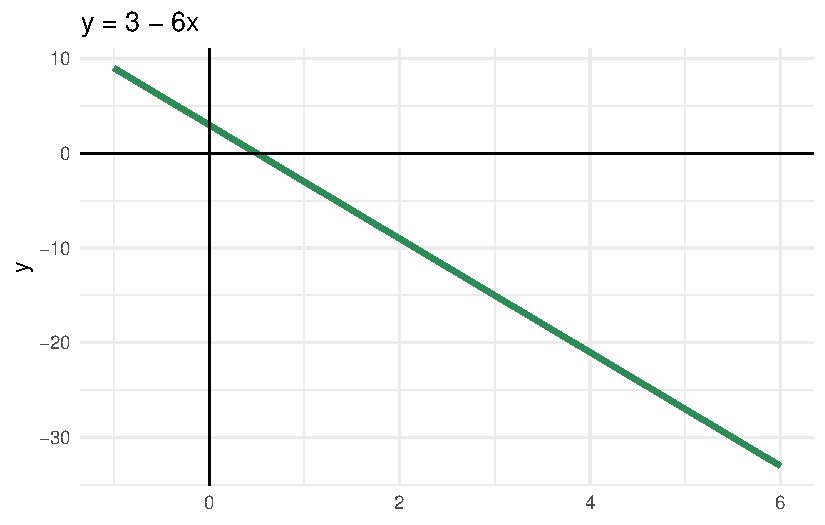
\includegraphics{Appendices/antwoorden_wiskunde_files/figure-pdf/fig-draw-1a-1.pdf}

}

\caption{\label{fig-draw-1a}Oefening 1a}

\end{figure}

\textbf{b.} \(y=px+q\)

1. Snijpunten met de x-as:\\
\(y = 0 \quad \Rightarrow \quad px + q = 0 \quad \Rightarrow \quad x = -\frac{q}{p}\)\\
2. Snijpunten met de y-as:\\
\(y = f(0) = p \cdot 0 + q = q\)\\
3. Horizontale asymptoten:\\
Geen.\\
4. Verticale asymptoten:\\
Geen.\\
5: Minima en maxima:\\
Geen.

\begin{figure}

{\centering 

\href{https://www.desmos.com/calculator/qogqwu8ugj}{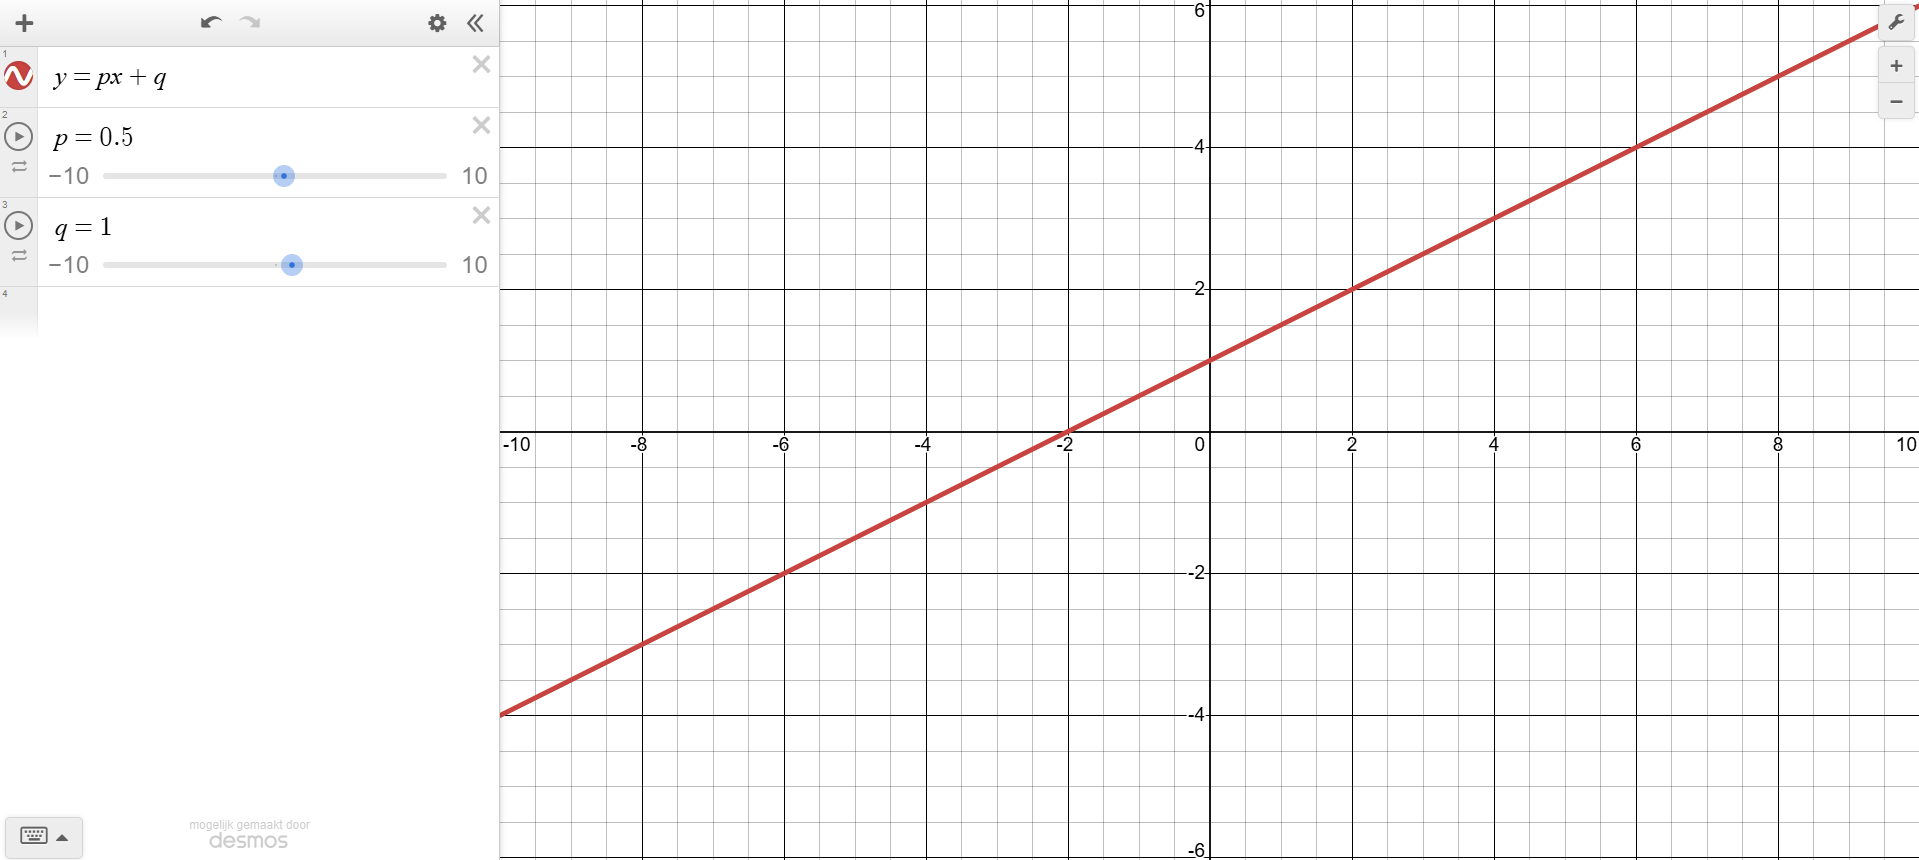
\includegraphics{Appendices/figuren/wis_ant_exr_draw_1b.png}}

}

\caption{Oefening 1b voor specifieke waarden van p en q. Klik op figuur
voor interactieve plot in Desmos}

\end{figure}

\textbf{c.} \(y=x-3x^2\)

1. Snijpunten met de x-as:\\
\(y = 0 \quad \Rightarrow \quad x(1 - 3x) = 0 \quad \Rightarrow \quad x = 0 \text{ of } x = \frac{1}{3}\)\\
2. Snijpunten met de y-as:\\
\(y = f(0) = 0 - 2\cdot 0^2 = 0\)\\
3. Horizontale asymptoten:\\
Geen.\\
4. Verticale asymptoten:\\
Geen.\\
5: Minima en maxima:\\
De afgeleide is \(f'(x) = 1 - 6x\).\\
Gelijkstellen aan 0 om de minima en maxima te bepalen:\\
\(f'(x) = 1 - 6x = 0\)\\
\(x = 1/6\)\\
De y-waarde op \(x = 1/6\) is:\\
\(f(1/6) = \frac{1}{6} - 3 \left( \frac{1}{6} \right)^2 = \frac{1}{6} - \frac{1}{12} = \frac{1}{12}\)

\begin{figure}

{\centering 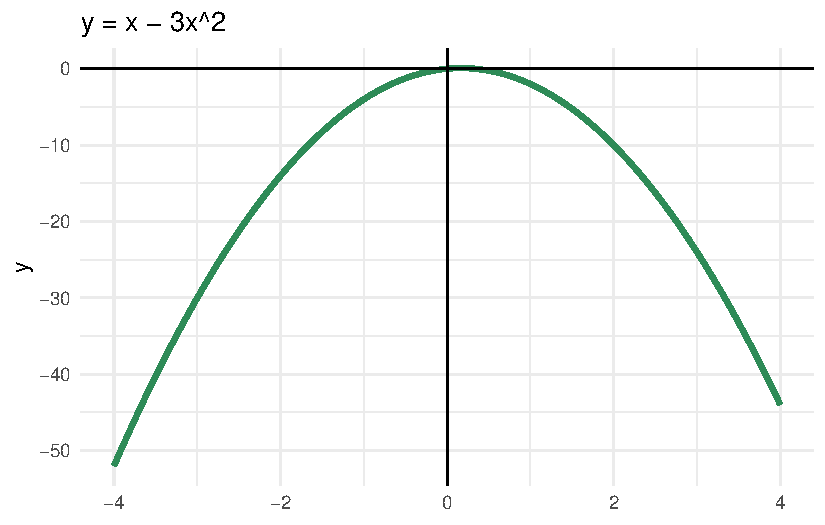
\includegraphics{Appendices/antwoorden_wiskunde_files/figure-pdf/fig-draw-1c-1.pdf}

}

\caption{\label{fig-draw-1c}Oefening 1c}

\end{figure}

\textbf{d.} \(y=(a-x) \cdot (b-x) \cdot (c-x)\)

1. Snijpunten met de x-as:\\
\(y = 0 \quad \Rightarrow \quad (a - x)(b - x)(c - x) = 0\)\\
Snijpunten op de x-as op: \(x=a\), \(x=b\) en \(x=c\).\\
2. Snijpunten met de y-as:\\
\(y = f(0) = (a-0) \cdot (b-0 \cdot (c-0) = abc\)\\
3. Horizontale asymptoten:\\
Geen.\\
4. Verticale asymptoten:\\
Geen.\\
5: Minima en maxima:\\
Tussen de snijpunten met de x-as, afhankelijk van de waarden van \(a\),
\(b\) en \(c\).

\begin{figure}

{\centering 

\href{https://www.desmos.com/calculator/fegtbefznv}{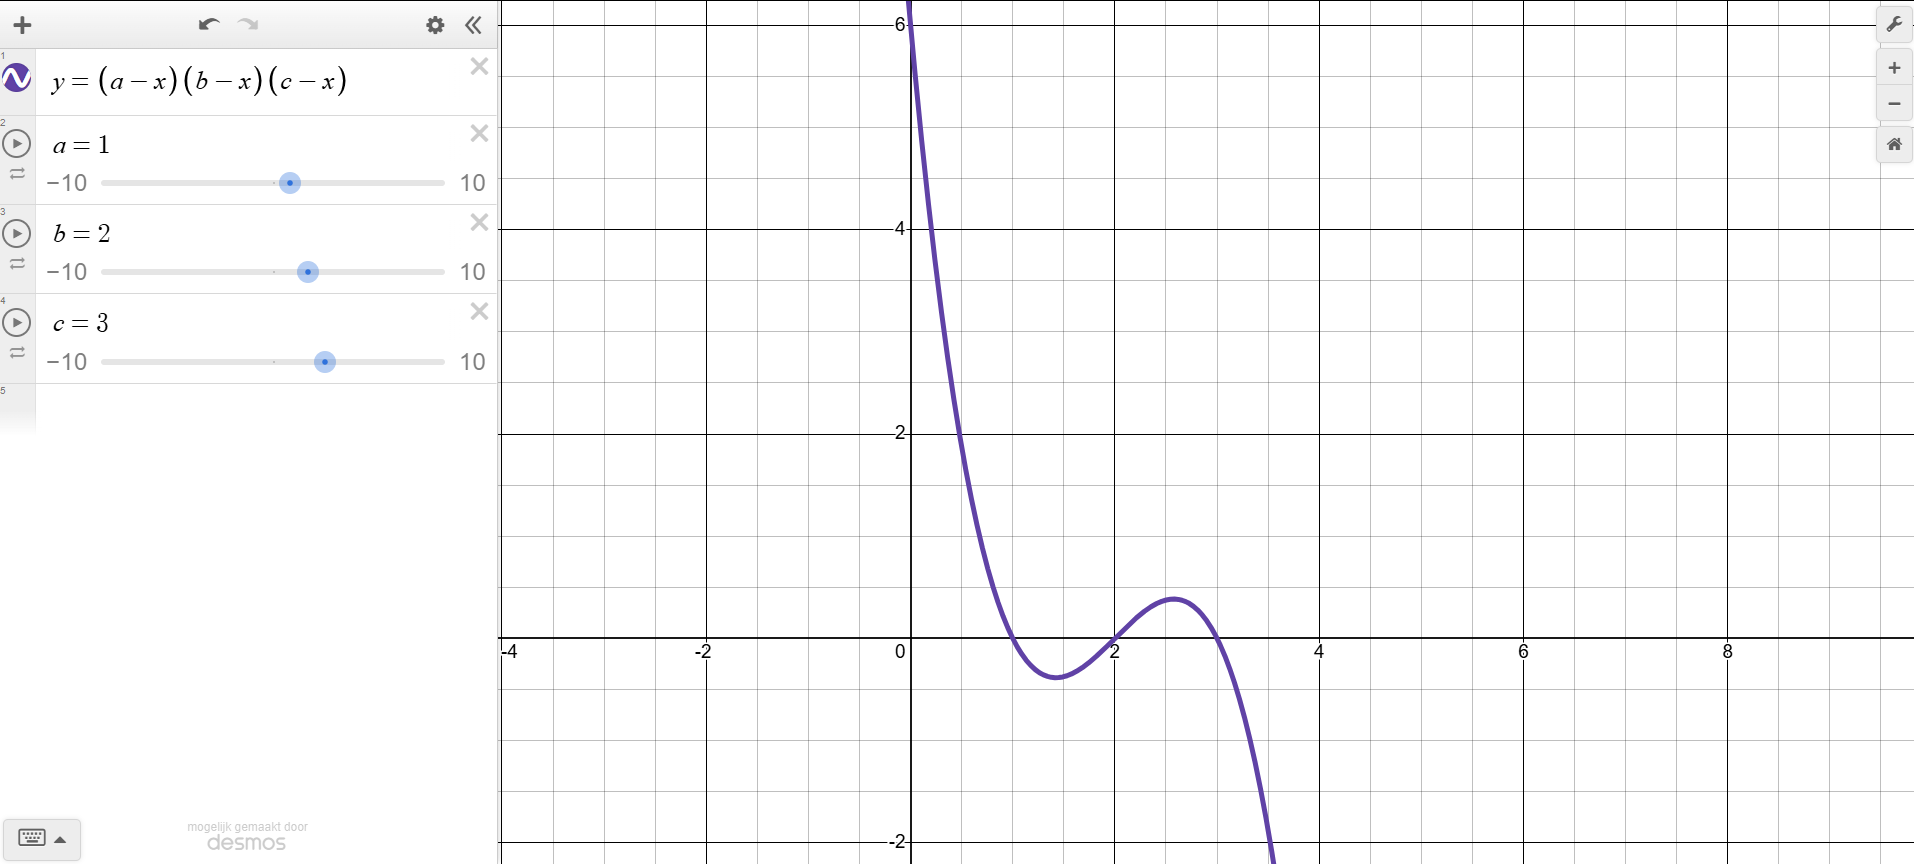
\includegraphics{Appendices/figuren/wis_ant_exr_draw_1d.png}}

}

\caption{Oefening 1d voor specifieke waarden van a, b en c.~Klik op
figuur voor interactieve plot in Desmos}

\end{figure}

\textbf{e.} \(y=x^3-5x^2\)

1. Snijpunten met de x-as:\\
\(y = 0 \quad \Rightarrow \quad x^2(x - 5) = 0 \quad \Rightarrow \quad x = 0 \text{ of } x = 5\)\\
2. Snijpunten met de y-as:\\
\(y = f(0) = 0^3 - 5 \cdot 0^2 = 0\)\\
3. Horizontale asymptoten:\\
Voor \(y = \lim x \to + \infty\) geldt dat \(y \to + \infty\).\\
Voor \(y = \lim x \to - \infty\) geldt dat \(y \to - \infty\).\\
4. Verticale asymptoten:\\
Geen.\\
5: Minima en maxima:\\
De afgeleide is \(f'(x) = 3x^2 - 10x\).\\
Gelijkstellen aan 0 om de minima en maxima te bepalen:\\
\(f'(x) = 3x^2 - 10x = 0\)\\
\(x(3x - 10) = 0\)\\
\(x = 0\) of \(3x = 10 \quad \Rightarrow \quad x = 10/3\)\\
De y-waarde op \(x = 0\) is:\\
\(f(0) = 0\)\\
De y-waarde op \(x = 10/3\) is:\\
\(f(\frac{10}{3}) = (\frac{10}{3})^3-5\cdot(\frac{10}{3})^2 = - \frac{500}{27}\)

\begin{figure}

{\centering 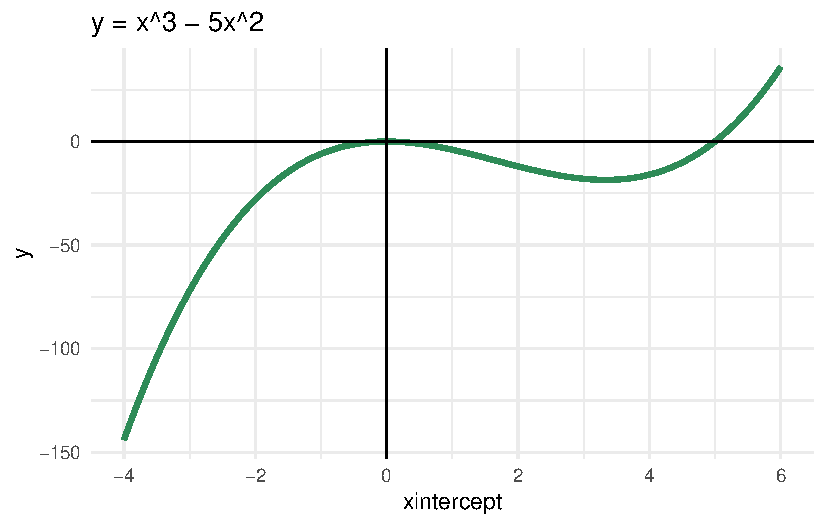
\includegraphics{Appendices/antwoorden_wiskunde_files/figure-pdf/fig-draw-1e-1.pdf}

}

\caption{\label{fig-draw-1e}Oefening 1e}

\end{figure}

\textbf{f.} \(y=\frac{4x}{x+2}+4\)

1. Snijpunten met de x-as:\\
\(y = 0 \quad \Rightarrow \quad \frac{4x}{x+2} + 4 = 0 \quad \Rightarrow \quad \frac{4x}{x+2} = -4\)\\
2. Snijpunten met de y-as:\\
\(y = f(0) = \frac{4\cdot0}{0+2}+4 = 4\)\\
3. Horizontale asymptoten:\\
Dit is een rationale functie, dus we kunnen het stappenplan daarvoor
gebruiken:\\
\hspace*{0.333em}\hspace*{0.333em}i) De hoogste macht van \(x\) is
\(x\).\\
\hspace*{0.333em}\hspace*{0.333em}ii) Delen door \(x\) geeft
\(\frac{\frac{4x}{x}}{\frac{x}{x}+\frac{2}{x}}+4 = \frac{4}{1+\frac{2}{x}}+4\).\\
\hspace*{0.333em}\hspace*{0.333em}iii) De limiet wordt dan:
\(\frac{4}{1+0} + 4 = 8\)\\
4. Verticale asymptoten:\\
Er is sprake van een verticale asymptoot als er een waarde voor \(x\) is
waarbij de noemer 0 is, dus \(x+2 = 0 \Rightarrow x = -2\)\\
5: Minima en maxima:\\
De afgeleide is \(f'(x) = \frac{8}{(x+2)^2}\). Dit kan nooit gelijk zijn
aan 0, dus deze functie heeft geen minima of maxima.

\begin{verbatim}
Warning: Removed 91 rows containing missing values or values outside the scale range
(`geom_line()`).
\end{verbatim}

\begin{verbatim}
Warning: Removed 38 rows containing missing values or values outside the scale range
(`geom_line()`).
\end{verbatim}

\begin{figure}

{\centering 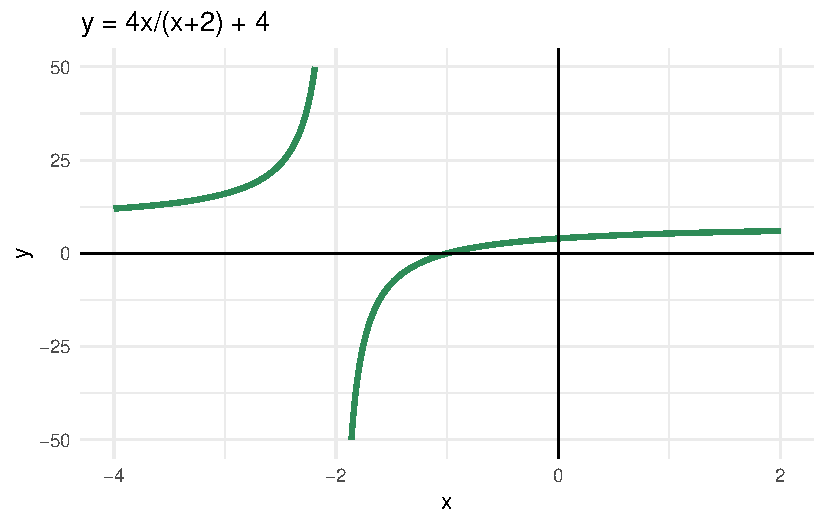
\includegraphics{Appendices/antwoorden_wiskunde_files/figure-pdf/fig-draw-1f-1.pdf}

}

\caption{\label{fig-draw-1f}Oefening 1f}

\end{figure}

Oefening~\ref{exr-draw-2}

\textbf{a.}

Als er geen vossen zijn, geldt \(V=0\), dus:

\(K=a-b\cdot0\)\\
\(K=a\)\\
Het aantal konijnen \(K\) is dan gelijk aan \(a\). Als er wel vossen
zouden zijn, wordt de negatieve term \(b\cdot V\) groter. Het aantal
konijnen neemt dan af en zal in aanwezigheid van vossen dus altijd
kleiner zijn dan \(a\).

\textbf{b.}

\begin{figure}

{\centering 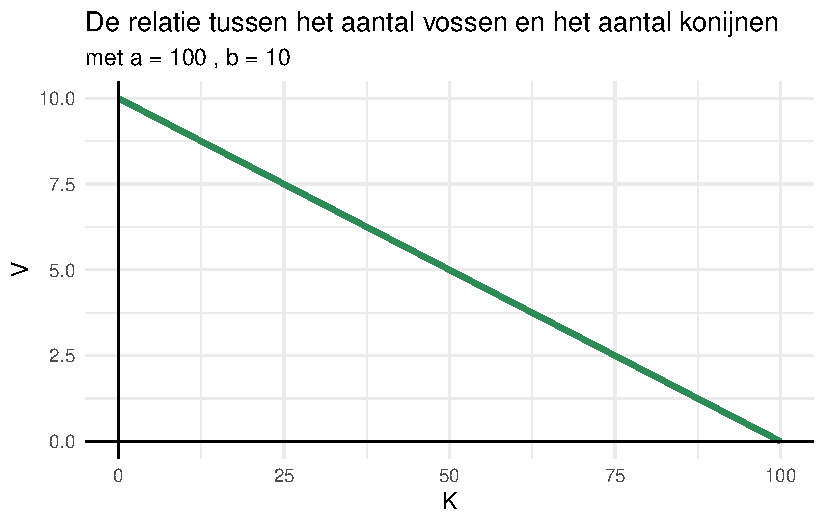
\includegraphics{Appendices/antwoorden_wiskunde_files/figure-pdf/fig-draw-2b-1.pdf}

}

\caption{\label{fig-draw-2b}Oefening 2b}

\end{figure}

\textbf{c.}

\(K = a - b\cdot V\)\\
\(K + b\cdot V =a\)\\
\(b\cdot V = a - K\)\\
\(V = \frac{a-K}{b}\)\\
Het schetsen van deze functie geeft precies dezelfde grafiek als in b.

\textbf{d.}

Het maakt niet uit of je de functie herschrijft, de grafiek ziet er
precies hetzelfde uit als de assen hetzelfde bijven. Vaak is het echter
wel het makkelijkste om de grafiek te tekenen als je de variabele die je
op de y-as wilt zetten (dus de vossen in dit geval) aan de linkerkant in
de formule hebt staan, zoals het geval is in opdracht c.~Het kan daarom
nuttig zijn om een functie te herschrijven, maar het verandert niks aan
de uitkomst.

\hypertarget{antwoorden-r}{%
\chapter*{Antwoorden R}\label{antwoorden-r}}
\addcontentsline{toc}{chapter}{Antwoorden R}

\markboth{Antwoorden R}{Antwoorden R}

Oefening~\ref{exr-R-1}

\textbf{a.} Een matrix is een tabel met allemaal dezelfde type waarden,
terwijl een dataframe voor elke kolom een ander type data kan bevatten.

\textbf{b.} De tweede waarde van de vector x is 1.5.

\begin{Shaded}
\begin{Highlighting}[]
\NormalTok{x }\OtherTok{\textless{}{-}} \FunctionTok{seq}\NormalTok{(}\DecValTok{1}\NormalTok{,}\DecValTok{10}\NormalTok{,}\AttributeTok{by=}\FloatTok{0.5}\NormalTok{)}
\NormalTok{x[}\DecValTok{2}\NormalTok{]}
\end{Highlighting}
\end{Shaded}

\textbf{c.} De vector x bevat nu alle gehele getallen van 10 tot en met
1. De eerste waarde van deze vector is 10.

\begin{Shaded}
\begin{Highlighting}[]
\NormalTok{x }\OtherTok{\textless{}{-}} \DecValTok{10}\SpecialCharTok{:}\DecValTok{1}
\NormalTok{x[}\DecValTok{1}\NormalTok{] }
\end{Highlighting}
\end{Shaded}

\textbf{d.} x{[}1{]} weet je niet, want runif geeft willekeurig
getallen. Je weet wél dat het getal tussen 0 en 1 zal liggen. x{[}11{]}
bestaat niet, want er zijn maar 10 getallen gegenereerd R geeft in dit
geval `NA' (not available).

\textbf{e.}

\begin{Shaded}
\begin{Highlighting}[]
\NormalTok{df}\SpecialCharTok{$}\NormalTok{score\_per\_minuut }\OtherTok{\textless{}{-}}\NormalTok{ df}\SpecialCharTok{$}\NormalTok{score}\SpecialCharTok{/}\NormalTok{df}\SpecialCharTok{$}\NormalTok{minuten}
\end{Highlighting}
\end{Shaded}

\textbf{f.} dieren{[}2,3:4{]} geeft rij 2, kolom 3 en 4 terug. Let op:
de eerste regel zijn de kolomnamen, dus de 2e rij is niet Joey, maar
Roos! Daarom geeft dieren{[}2,3:4{]} de waarden ``wit'' en ``energiek''.

\textbf{g.} De waarde begint op 1, en er wordt eerst 1, dan 2, en dan
nog 3 bij opgeteld. Aan het einde is a dus 1+1+2+3 = 7.

Oefening~\ref{exr-R-2}

\textbf{a.}

\begin{Shaded}
\begin{Highlighting}[]
\CommentTok{\# waarden instellen}
\NormalTok{a }\OtherTok{\textless{}{-}} \FloatTok{2.5}
\NormalTok{b }\OtherTok{\textless{}{-}} \DecValTok{11}
\NormalTok{c }\OtherTok{\textless{}{-}} \FloatTok{0.01}

\CommentTok{\# bereken de uitkomst}
\NormalTok{uitkomst }\OtherTok{\textless{}{-}}\NormalTok{ a}\SpecialCharTok{/}\NormalTok{b}\SpecialCharTok{+}\NormalTok{a}\SpecialCharTok{*}\NormalTok{(c}\SpecialCharTok{+}\NormalTok{a)}

\NormalTok{a }\OtherTok{\textless{}{-}} \DecValTok{5}
\end{Highlighting}
\end{Shaded}

\textbf{b.} Bij het berekenen van uitkomst worden de parameters a, b, en
c\\
gebruikt om iets te berekenen. Dit komt neer op pasta, groente, en pesto
combineren in een gerecht. Dat je daarna de pesto aanpast verandert niet
je gerecht: die was al klaar.

Oefening~\ref{exr-R-3}

\textbf{a.} Vijf kolommen. Dit is geen CSV (comma-separated-values)
bestand, want de kolommen zijn gescheiden door spaties, niet komma's.

\textbf{b.}

\begin{Shaded}
\begin{Highlighting}[]
\FunctionTok{nrow}\NormalTok{(covid) }\CommentTok{\# 52, dus dat klopt}
\FunctionTok{ncol}\NormalTok{(covid) }\CommentTok{\# 1, dit is fout! Alle data wordt als 1 kolom ingelezen.}
\end{Highlighting}
\end{Shaded}

\textbf{c.}

\begin{Shaded}
\begin{Highlighting}[]
\FunctionTok{ncol}\NormalTok{(covid) }\CommentTok{\# 5, precies goed!}
\FunctionTok{nrow}\NormalTok{(covid) }\CommentTok{\# 53, dat is 1 te veel... }
\FunctionTok{View}\NormalTok{(covid) }\CommentTok{\# Aha... de kolomnamen worden als "eerste rij" ingelezen...}
\end{Highlighting}
\end{Shaded}

\textbf{d.}

\begin{Shaded}
\begin{Highlighting}[]
\FunctionTok{mean}\NormalTok{(covid}\SpecialCharTok{$}\NormalTok{positieve\_testen) }\CommentTok{\# gemiddeld 1563.5 positieve testen per week}
\end{Highlighting}
\end{Shaded}

\textbf{e.}

\begin{Shaded}
\begin{Highlighting}[]
\FunctionTok{head}\NormalTok{(covid,}\AttributeTok{n=}\DecValTok{12}\NormalTok{)}
\end{Highlighting}
\end{Shaded}

\textbf{f.}

\begin{Shaded}
\begin{Highlighting}[]
\CommentTok{\# Lees het bestand covid.txt op de website in met \textquotesingle{}read.table\textquotesingle{}}
\NormalTok{covid }\OtherTok{\textless{}{-}} \FunctionTok{read.table}\NormalTok{(}\StringTok{"http://tbb.bio.uu.nl/bvd/bms/covid.txt"}\NormalTok{,}\AttributeTok{header=}\NormalTok{T)}
\FunctionTok{str}\NormalTok{(covid) }
\CommentTok{\# 5 rijen (observaties) en }
\CommentTok{\# 5 kolommen (variables), }
\CommentTok{\# allemaal van type \textquotesingle{}int\textquotesingle{} (integer: gehele getallen)}

\CommentTok{\# deze zelfde informatie kan je ook op andere manieren verkrijgen}
\FunctionTok{nrow}\NormalTok{(covid) }\CommentTok{\# 52}
\FunctionTok{ncol}\NormalTok{(covid) }\CommentTok{\# 5}
\FunctionTok{typeof}\NormalTok{(covid}\SpecialCharTok{$}\NormalTok{week) }\CommentTok{\# integer (geheel getal)}
\end{Highlighting}
\end{Shaded}

\textbf{g.}

\begin{Shaded}
\begin{Highlighting}[]
\CommentTok{\# Lees het bestand covid.txt op de website in met \textquotesingle{}read.table\textquotesingle{}}
\NormalTok{covid }\OtherTok{\textless{}{-}} \FunctionTok{read.table}\NormalTok{(}\StringTok{"http://tbb.bio.uu.nl/bvd/bms/covid.txt"}\NormalTok{,}\AttributeTok{header=}\NormalTok{T)}
\NormalTok{covid\_subset }\OtherTok{\textless{}{-}}\NormalTok{ covid[}\DecValTok{14}\SpecialCharTok{:}\DecValTok{19}\NormalTok{,] }\CommentTok{\# selecteer rij 14:19}

\NormalTok{x }\OtherTok{\textless{}{-}}\NormalTok{ covid\_subset}\SpecialCharTok{$}\NormalTok{datapunt }\CommentTok{\# alle x{-}punten in een vector}
\NormalTok{y }\OtherTok{\textless{}{-}}\NormalTok{ covid\_subset}\SpecialCharTok{$}\NormalTok{positieve\_testen }\CommentTok{\# alle y{-}punten in een vector}

\FunctionTok{plot}\NormalTok{(x,y, }\AttributeTok{type=}\StringTok{\textquotesingle{}b\textquotesingle{}}\NormalTok{,}\AttributeTok{lwd=}\DecValTok{2}\NormalTok{, }\AttributeTok{log=}\StringTok{"y"}\NormalTok{,}
     \AttributeTok{xlab=}\StringTok{"Datapunt"}\NormalTok{, }\AttributeTok{ylab=}\StringTok{"Aantal positieve testen (log{-}schaal)"}\NormalTok{,}
     \AttributeTok{col=}\StringTok{"darkblue"}\NormalTok{, }\AttributeTok{main=}\StringTok{"Aantal positieve Covid{-}19 testen in Utrecht"}\NormalTok{) }
\end{Highlighting}
\end{Shaded}

\textbf{h.}

\begin{Shaded}
\begin{Highlighting}[]
\NormalTok{covid }\OtherTok{\textless{}{-}} \FunctionTok{read.table}\NormalTok{(}\StringTok{"http://tbb.bio.uu.nl/bvd/bms/covid.txt"}\NormalTok{,}\AttributeTok{header=}\NormalTok{T)}
\NormalTok{x }\OtherTok{\textless{}{-}}\NormalTok{ covid}\SpecialCharTok{$}\NormalTok{datapunt }\CommentTok{\# alle x{-}punten in een vector}
\NormalTok{y }\OtherTok{\textless{}{-}}\NormalTok{ covid}\SpecialCharTok{$}\NormalTok{positieve\_testen }\CommentTok{\# alle y{-}punten in een vector}

\FunctionTok{plot}\NormalTok{(x,y, }\AttributeTok{type=}\StringTok{\textquotesingle{}b\textquotesingle{}}\NormalTok{,}\AttributeTok{lwd=}\DecValTok{2}\NormalTok{, }\AttributeTok{log=}\StringTok{"y"}\NormalTok{,}
     \AttributeTok{xlab=}\StringTok{"Datapunt"}\NormalTok{, }\AttributeTok{ylab=}\StringTok{"Aantal positieve testen (log{-}schaal)"}\NormalTok{,}
     \AttributeTok{col=}\StringTok{"darkblue"}\NormalTok{, }\AttributeTok{main=}\StringTok{"Aantal positieve Covid{-}19 testen in Utrecht}\SpecialCharTok{\textbackslash{}n}\StringTok{Dikkere punten geven pieken weer"}\NormalTok{) }


\NormalTok{covid\_subset }\OtherTok{\textless{}{-}}\NormalTok{ covid[covid}\SpecialCharTok{$}\NormalTok{positieve\_testen }\SpecialCharTok{\textgreater{}} \DecValTok{1000}\NormalTok{,]}
\NormalTok{x }\OtherTok{\textless{}{-}}\NormalTok{ covid\_subset}\SpecialCharTok{$}\NormalTok{datapunt }\CommentTok{\# alle x{-}punten in een vector}
\NormalTok{y }\OtherTok{\textless{}{-}}\NormalTok{ covid\_subset}\SpecialCharTok{$}\NormalTok{positieve\_testen }\CommentTok{\# alle y{-}punten in een vector}

\FunctionTok{points}\NormalTok{(x,y, }\AttributeTok{lwd=}\DecValTok{5}\NormalTok{, }\AttributeTok{log=}\StringTok{"y"}\NormalTok{, }\AttributeTok{col=}\StringTok{"darkblue"}\NormalTok{) }
\end{Highlighting}
\end{Shaded}

Oefening~\ref{exr-R-4}

\textbf{a.}

\begin{Shaded}
\begin{Highlighting}[]
\ControlFlowTok{for}\NormalTok{(i }\ControlFlowTok{in} \DecValTok{1}\SpecialCharTok{:}\DecValTok{12}\NormalTok{)\{}
\NormalTok{  dobbelsteen }\OtherTok{\textless{}{-}} \FunctionTok{sample}\NormalTok{(}\DecValTok{1}\SpecialCharTok{:}\DecValTok{6}\NormalTok{,}\DecValTok{1}\NormalTok{) }\CommentTok{\# getal van 1 t/m 6 (dobbelsteen worp)}
  \ControlFlowTok{if}\NormalTok{(dobbelsteen}\SpecialCharTok{\textgreater{}=}\DecValTok{4}\NormalTok{) }\FunctionTok{cat}\NormalTok{(}\FunctionTok{paste}\NormalTok{(}\StringTok{"Worp nummer"}\NormalTok{,i,}\StringTok{"is"}\NormalTok{,dobbelsteen,}\StringTok{"}\SpecialCharTok{\textbackslash{}n}\StringTok{"}\NormalTok{))}
\NormalTok{\}}
\end{Highlighting}
\end{Shaded}

\textbf{b.}

\begin{Shaded}
\begin{Highlighting}[]
\NormalTok{aantal\_keren\_hoera }\OtherTok{\textless{}{-}} \DecValTok{0}
\ControlFlowTok{for}\NormalTok{(e }\ControlFlowTok{in} \DecValTok{1}\SpecialCharTok{:}\DecValTok{100}\NormalTok{)\{}
\NormalTok{  aantal\_keren\_6 }\OtherTok{\textless{}{-}} \DecValTok{0}
  \ControlFlowTok{for}\NormalTok{(i }\ControlFlowTok{in} \DecValTok{1}\SpecialCharTok{:}\DecValTok{12}\NormalTok{)\{}
\NormalTok{    dobbelsteen }\OtherTok{\textless{}{-}} \FunctionTok{sample}\NormalTok{(}\DecValTok{1}\SpecialCharTok{:}\DecValTok{6}\NormalTok{,}\DecValTok{1}\NormalTok{) }\CommentTok{\# getal van 1 t/m 6 (dobbelsteen worp)}
    \ControlFlowTok{if}\NormalTok{(dobbelsteen }\SpecialCharTok{==}\DecValTok{6}\NormalTok{) aantal\_keren\_6 }\OtherTok{\textless{}{-}}\NormalTok{ aantal\_keren\_6 }\SpecialCharTok{+} \DecValTok{1}
\NormalTok{  \}}
  \ControlFlowTok{if}\NormalTok{(aantal\_keren\_6}\SpecialCharTok{==}\DecValTok{1}\NormalTok{) \{}
    \FunctionTok{cat}\NormalTok{(}\StringTok{"Hoera!}\SpecialCharTok{\textbackslash{}n}\StringTok{"}\NormalTok{)}
\NormalTok{    aantal\_keren\_hoera }\OtherTok{\textless{}{-}}\NormalTok{ aantal\_keren\_hoera }\SpecialCharTok{+} \DecValTok{1}
\NormalTok{  \}}
  \ControlFlowTok{else}\NormalTok{\{}
    \FunctionTok{cat}\NormalTok{(}\StringTok{"Niet hoera :(}\SpecialCharTok{\textbackslash{}n}\StringTok{"}\NormalTok{)}
\NormalTok{  \}}
\NormalTok{\}}
\FunctionTok{cat}\NormalTok{(}\StringTok{"Er is in totaal"}\NormalTok{, aantal\_keren\_hoera, }\StringTok{"keer \textquotesingle{}Hoera!\textquotesingle{} geprint}\SpecialCharTok{\textbackslash{}n}\StringTok{"}\NormalTok{)}
\end{Highlighting}
\end{Shaded}

\hypertarget{antwoorden-modelleren}{%
\chapter*{Antwoorden modelleren}\label{antwoorden-modelleren}}
\addcontentsline{toc}{chapter}{Antwoorden modelleren}

\markboth{Antwoorden modelleren}{Antwoorden modelleren}

\textbf{a.}

\textbf{b.}

\textbf{c.}

\textbf{d.}

\textbf{e.}

\textbf{f.}

\textbf{g.}

\textbf{h.}

\hypertarget{antwoorden-sec-tbintro}{%
\section*{\texorpdfstring{Antwoorden
Hoofdstuk~\ref{sec-tbintro}}{Antwoorden Hoofdstuk~}}\label{antwoorden-sec-tbintro}}
\addcontentsline{toc}{section}{Antwoorden Hoofdstuk~\ref{sec-tbintro}}

\markright{Antwoorden Hoofdstuk~\ref{sec-tbintro}}

Oefening~\ref{exr-variabelen-en-parameters}

\textbf{a.} De dingen die veranderen (bijvoorbeeld over de tijd) noemen
we variabelen. De dingen die veranderen zijn hier je bloedsuikerspiegel
(a) en de hoeveelheid eiwit (c), dus dit zou je de variabelen kunnen
noemen.

\textbf{b.} De snelheden (b en d) waarmee de variabelen veranderen,
staan volgens de omschrijving vast, en zijn daarom parameters.

Oefening~\ref{exr-modeluitkomsten}

\textbf{a.} Eén van de aannames van een ODE-model is dat het systeem
goed gemengd is (Figuur~\ref{fig-modeltypes} B). Naast de groeisnelheid
is de ruimtelijke structuur bij een biofilm ook relevant. Hierom is het
beter om een ruimtelijk model te gebruiken voor het modelleren van een
biofilm.

\textbf{b.} Door goed te mengen zijn posities niet belangrijk, dus het
modelleren van posities is niet inzichtelijk. Het is beter om dit
systeem met bijvoorbeeld een ODE te beschrijven.

\textbf{c.} De vorming van korstmossen is een proces waarbij
posities/ruimte belangrijk is, dus een ruimtelijk model is het meest
geschikt.

\hypertarget{antwoorden-sec-exp}{%
\section*{\texorpdfstring{Antwoorden
Hoofdstuk~\ref{sec-exp}}{Antwoorden Hoofdstuk~}}\label{antwoorden-sec-exp}}
\addcontentsline{toc}{section}{Antwoorden Hoofdstuk~\ref{sec-exp}}

\markright{Antwoorden Hoofdstuk~\ref{sec-exp}}

Oefening~\ref{exr-exponentiele-groei-langzaam}

\textbf{a.} Ja, het percentage is klein maar is alsnog exponentieel!!
Dit kun je ook zien doordat de hoeveelheid rijst per vakje met een
rechte lijn toeneemt op een log-lineaire schaal.

\begin{Shaded}
\begin{Highlighting}[]
\CommentTok{\# beginaantal rijst}
\NormalTok{R }\OtherTok{\textless{}{-}} \DecValTok{1}

\CommentTok{\# herhaal iets 63 keer met een for{-}loop}
\ControlFlowTok{for}\NormalTok{ (i }\ControlFlowTok{in} \DecValTok{1}\SpecialCharTok{:}\DecValTok{63}\NormalTok{) \{}
\NormalTok{  R[i}\SpecialCharTok{+}\DecValTok{1}\NormalTok{] }\OtherTok{\textless{}{-}}\NormalTok{ R[i]}\SpecialCharTok{*}\FloatTok{1.05} \CommentTok{\# R in volgende stap is 2*R in deze stap}
\NormalTok{\}}

\FunctionTok{plot}\NormalTok{(R , }\AttributeTok{type=}\StringTok{\textquotesingle{}l\textquotesingle{}}\NormalTok{, }\AttributeTok{col=}\StringTok{"seagreen"}\NormalTok{, }\AttributeTok{log=}\StringTok{"y"}\NormalTok{, }\AttributeTok{lwd=}\DecValTok{2}\NormalTok{) }
\end{Highlighting}
\end{Shaded}

\begin{figure}[H]

{\centering 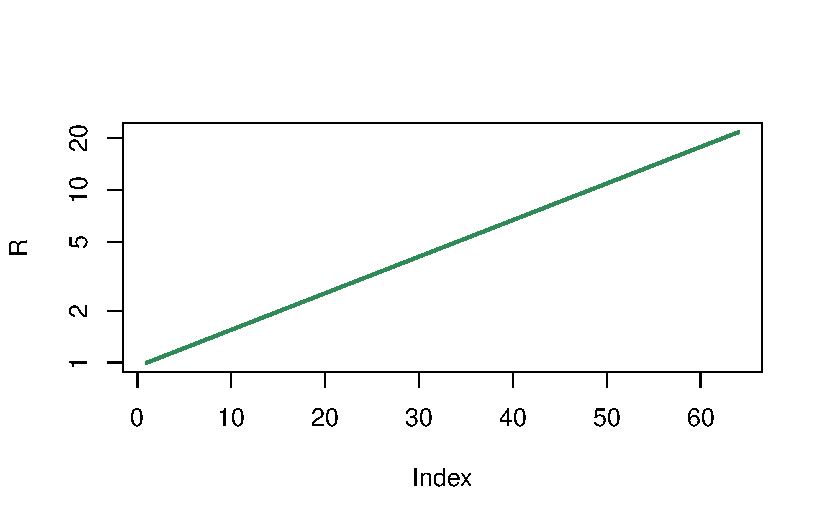
\includegraphics{Appendices/antwoorden_modelleren_files/figure-pdf/fig-exponential-1.pdf}

}

\caption{\label{fig-exponential}\textbf{?(caption)}}

\end{figure}

\textbf{b.} Door de rijstkorrels in elke vakje bij elkaar op te tellen
kunnen we uitrekenen hoeveel rijstkorrels je in totaal hebt:

\begin{Shaded}
\begin{Highlighting}[]
\FunctionTok{sum}\NormalTok{(R)}
\end{Highlighting}
\end{Shaded}

\begin{verbatim}
[1] 434.0933
\end{verbatim}

Oefening~\ref{exr-rabbits-map}

\textbf{a.}

\begin{Shaded}
\begin{Highlighting}[]
\CommentTok{\# definieren van begin aantal konijnen}
\NormalTok{konijnen }\OtherTok{\textless{}{-}} \DecValTok{24}
\CommentTok{\# verdubbel het aantal konijnen 20 keer}
\ControlFlowTok{for}\NormalTok{ (i }\ControlFlowTok{in} \DecValTok{1}\SpecialCharTok{:}\DecValTok{20}\NormalTok{)\{ }
\NormalTok{konijnen }\OtherTok{\textless{}{-}}\NormalTok{ konijnen }\SpecialCharTok{*} \DecValTok{2}
\NormalTok{\}}
\CommentTok{\# er zijn verschillende opties om "Het aantal konijnen na 20 tijdstappen is gelijk aan 25165824” te printen:}
\CommentTok{\# met cat:}
\FunctionTok{cat}\NormalTok{(}\StringTok{"Het aantal konijnen na 20 tijdstappen is gelijk aan "}\NormalTok{, konijnen)}
\end{Highlighting}
\end{Shaded}

\begin{verbatim}
Het aantal konijnen na 20 tijdstappen is gelijk aan  25165824
\end{verbatim}

\begin{Shaded}
\begin{Highlighting}[]
\CommentTok{\# met paste:}
\FunctionTok{paste}\NormalTok{(}\StringTok{"Het aantal konijnen na 20 tijdstappen is gelijk aan "}\NormalTok{, konijnen)}
\end{Highlighting}
\end{Shaded}

\begin{verbatim}
[1] "Het aantal konijnen na 20 tijdstappen is gelijk aan  25165824"
\end{verbatim}

\textbf{b.}

\begin{Shaded}
\begin{Highlighting}[]
\CommentTok{\# Stap 1: Stel begin{-}aantal konijnen in}
\NormalTok{konijnen }\OtherTok{\textless{}{-}} \DecValTok{24}

\CommentTok{\# Stap 2: Verdubbel het aantal konijnen 30 keer}
\ControlFlowTok{for}\NormalTok{ (t }\ControlFlowTok{in} \DecValTok{1}\SpecialCharTok{:}\DecValTok{30}\NormalTok{)\{}
\NormalTok{  konijnen[t}\SpecialCharTok{+}\DecValTok{1}\NormalTok{] }\OtherTok{\textless{}{-}} \DecValTok{2}\SpecialCharTok{*}\NormalTok{konijnen[t]}
\NormalTok{\}}

\CommentTok{\# Stap 3: Plot het resultaat}
\FunctionTok{plot}\NormalTok{(konijnen, }\AttributeTok{type=}\StringTok{\textquotesingle{}l\textquotesingle{}}\NormalTok{, }\AttributeTok{col=}\StringTok{"seagreen"}\NormalTok{)}
\end{Highlighting}
\end{Shaded}

\begin{figure}[H]

{\centering 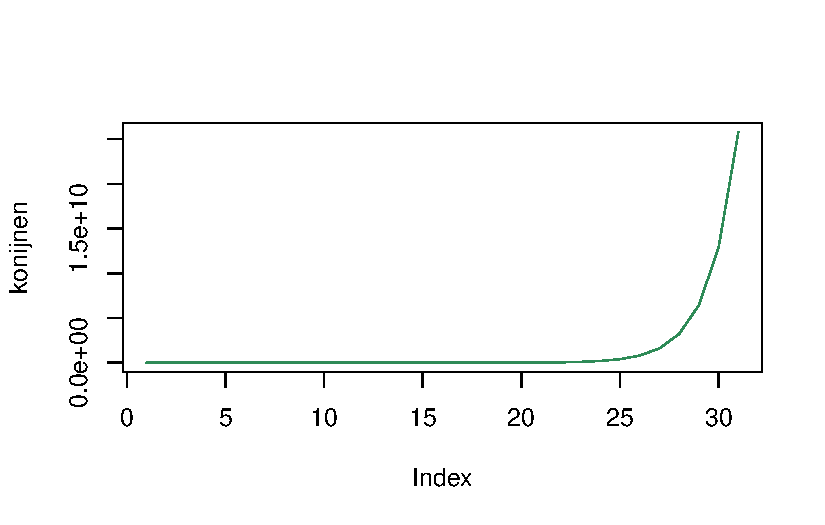
\includegraphics{Appendices/antwoorden_modelleren_files/figure-pdf/unnamed-chunk-4-1.pdf}

}

\end{figure}

De toename van het aantal konijnen lijkt exponentieel te zijn. Door de
y-as log-lineair te maken kunnen we dit zeker weten:

\begin{Shaded}
\begin{Highlighting}[]
\CommentTok{\# Stap 1: Stel begin {-}aantal konijnen in}
\NormalTok{konijnen }\OtherTok{\textless{}{-}} \DecValTok{24}
\CommentTok{\# Stap 2: Verdubbel het aantal konijnen 30 keer}
\ControlFlowTok{for}\NormalTok{ (t }\ControlFlowTok{in} \DecValTok{1}\SpecialCharTok{:}\DecValTok{30}\NormalTok{)\{}
\NormalTok{konijnen [t}\SpecialCharTok{+}\DecValTok{1}\NormalTok{] }\OtherTok{\textless{}{-}} \DecValTok{2}\SpecialCharTok{*}\NormalTok{ konijnen [t]}
\NormalTok{\}}
\CommentTok{\# Stap 3: Plot het resultaat met een logaritmische y as, net zoals in de code van figuur 3}
\FunctionTok{plot}\NormalTok{(konijnen , }\AttributeTok{type=}\StringTok{\textquotesingle{}l\textquotesingle{}}\NormalTok{, }\AttributeTok{col=}\StringTok{"seagreen"}\NormalTok{, }\AttributeTok{log=}\StringTok{"y"}\NormalTok{)}
\end{Highlighting}
\end{Shaded}

\begin{figure}[H]

{\centering 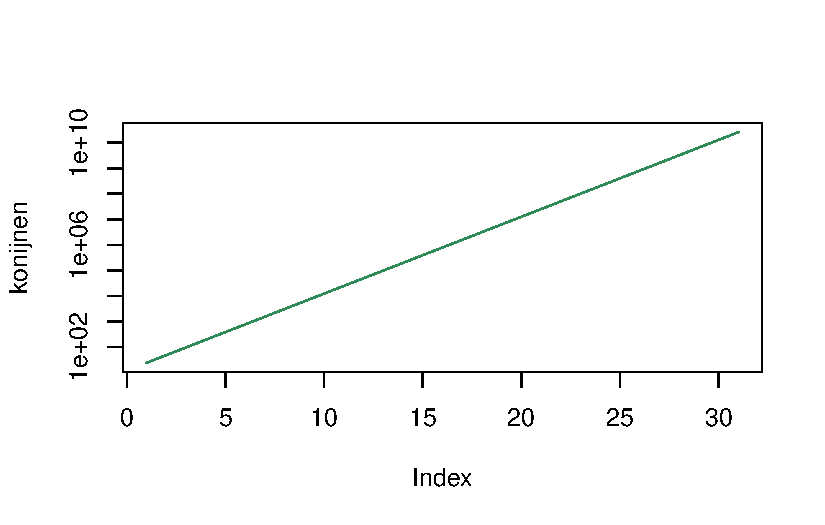
\includegraphics{Appendices/antwoorden_modelleren_files/figure-pdf/unnamed-chunk-5-1.pdf}

}

\end{figure}

Met een logaritmische schaal op de y-as krijgen we een rechte lijnen en
weten we nu zeker dat we met exponentiële groei te maken hebben.

\textbf{c.} :::\{\#todo-yannick\} LaTex code antwoorden invoegen.

\textbf{d.}

\textbf{e.}

\textbf{f.}

\textbf{g.}

\textbf{h.}


\backmatter

\end{document}
